%Este trabalho está licenciado sob a Licença Creative Commons Atribuição-CompartilhaIgual 3.0 Não Adaptada. Para ver uma cópia desta licença, visite https://creativecommons.org/licenses/by-sa/3.0/ ou envie uma carta para Creative Commons, PO Box 1866, Mountain View, CA 94042, USA.

%%%%%%%%%%%%%%%%%%%%%%%%%%%%%%%%%%%%%%%%%%
% ATENÇÃO
%
% POR SEGURANÇA, NÃO EDITE ESTE ARQUIVO
%
%%%%%%%%%%%%%%%%%%%%%%%%%%%%%%%%%%%%%%%%%

\documentclass[12pt]{book}

\input preambulo.tex

\begin{document}

\frontmatter

%titlepage
\ifisscilab
\title{Cálculo Numérico\\\small{Um Livro Colaborativo}\\\small{Versão Scilab}}
\fi
\ifisoctave
\title{Cálculo Numérico\\\small{Um Livro Colaborativo}\\\small{Versão Octave}}
\fi
\ifispython
\title{Cálculo Numérico\\\small{Um Livro Colaborativo}\\\small{Versão Python}}
\fi
\author{}
\ifishtml
\date{\today}
\else
\date{\today\vspace{1cm}\\\small{Veja a página do projeto em:\\
\url{https://www.ufrgs.br/reamat}
}
}
\fi
\ifishtml
\else
\addcontentsline{toc}{chapter}{Capa}
\fi

\ifishtml
\else
\AddToShipoutPicture*{\BackgroundPic}
\fi
\maketitle

%Este trabalho está licenciado sob a Licença Creative Commons Atribuição-CompartilhaIgual 3.0 Não Adaptada. Para ver uma cópia desta licença, visite https://creativecommons.org/licenses/by-sa/3.0/ ou envie uma carta para Creative Commons, PO Box 1866, Mountain View, CA 94042, USA.

\chapter*{Organizadores}
\addcontentsline{toc}{chapter}{Organizadores}

\begin{itemize}
\item[] Dagoberto Adriano Rizzotto Justo - UFRGS
\item[] Esequia Sauter - UFRGS
\item[] Fabio Souto de Azevedo - UFRGS
\item[] Leonardo Fernandes Guidi - UFRGS
\item[] Pedro Henrique de Almeida Konzen - UFRGS
\end{itemize}
%Este trabalho está licenciado sob a Licença Creative Commons Atribuição-CompartilhaIgual 3.0 Não Adaptada. Para ver uma cópia desta licença, visite https://creativecommons.org/licenses/by-sa/3.0/ ou envie uma carta para Creative Commons, PO Box 1866, Mountain View, CA 94042, USA.

\chapter*{Colaboradores}
\addcontentsline{toc}{chapter}{Colaboradores}

Este material é fruto da escrita colaborativa. Veja a lista de colaboradores em:
\begin{center}
  \url{https://github.com/reamat/CalculoNumerico/graphs/contributors}
\end{center}

Para saber mais como participar, visite o site oficial do projeto:
\begin{center}
  \url{https://www.ufrgs.br/reamat/CalculoNumerico}
\end{center}
ou comece agora mesmo visitando nosso repositório GitHub:
\begin{center}
  \url{https://github.com/reamat/CalculoNumerico}
\end{center}


% Aqui você encontra a lista de colaboradores do livro. Esta lista contém somente aqueles que explicitamente se manifestaram a favor de terem seus nomes registrados aqui. A lista completa de colaborações pode ser obtida no repositório GitHub do livro:
% \begin{center}
%   \url{https://github.com/livroscolaborativos/CalculoNumerico}
% \end{center}
% Além das colaborações via GitHub, o livro também recebe colaborações via discussões, sugestões e avisos deixados em nossa lista de e-mails:
% \begin{center}
% \url{livro_colaborativo@googlegroups.com}
% \end{center}
% Estas colaborações não estão listadas aqui, mas podem ser vistas no site do grupo de e-mails.

% Caso encontre algum equívoco ou veja seu nome listado aqui por engano, por favor, entre em contato conosco por e-mail:
% \begin{center}
%   \url{livroscolaborativos@gmail.com}
% \end{center}
% ou via o repositório GitHub.

% \begin{table}[h!]
%   \centering
%   \caption{Lista de colaboradores}
%   \label{tab:colaboradores}
%   \begin{tabular}{llll} \hline
%     Nome & Afiliação & E-Mail & 1ª Contribuição\\ \hline
%     Rafael Sachetto Oliveira & Universidade Federal de São João del-Rei & sachetto@ufsj.edu.br & \#158 \\
%     Debora Lidia Gisch & -x- & -x- & \#63 \\
%     \hline
%   \end{tabular}
% \end{table}

%Este trabalho está licenciado sob a Licença Creative Commons Atribuição-CompartilhaIgual 3.0 Não Adaptada. Para ver uma cópia desta licença, visite https://creativecommons.org/licenses/by-sa/3.0/ ou envie uma carta para Creative Commons, PO Box 1866, Mountain View, CA 94042, USA.

\chapter*{Licença}
\addcontentsline{toc}{chapter}{Licença}

Este trabalho está licenciado sob a Licença Creative Commons Atribuição-CompartilhaIgual 3.0 Não Adaptada. Para ver uma cópia desta licença, visite \url{https://creativecommons.org/licenses/by-sa/3.0/} ou envie uma carta para Creative Commons, PO Box 1866, Mountain View, CA 94042, USA.

%Este trabalho está licenciado sob a Licença Creative Commons Atribuição-CompartilhaIgual 3.0 Não Adaptada. Para ver uma cópia desta licença, visite https://creativecommons.org/licenses/by-sa/3.0/ ou envie uma carta para Creative Commons, PO Box 1866, Mountain View, CA 94042, USA.

\chapter*{Nota dos organizadores}
\addcontentsline{toc}{chapter}{Nota dos organizadores}

Nosso objetivo é de fomentar o desenvolvimento de materiais didáticos pela colaboração entre professores e alunos de universidades, institutos de educação e demais interessados no estudo e aplicação de cálculo numérico nos mais diversos ramos da ciência e tecnologia.

Para tanto, disponibilizamos em repositório público GitHub todo o código-fonte dos materiais em desenvolvimento sob licença Creative Commons Atribuição-CompartilhaIgual 3.0 Não Adaptada (\href{https://creativecommons.org/licenses/by-sa/3.0/}{CC-BY-SA-3.0}). Ou seja, você pode copiar, redistribuir, alterar e construir um novo material para qualquer uso, inclusive comercial. Leia a licença para maiores informações.

O sucesso do projeto depende da colaboração! Participe diretamenta da escrita dos recursos educacionais, dê sugestões ou nos avise de erros e imprecisões. Toda a colaboração é bem-vinda. Veja mais sobre o projeto em:
\begin{center}
  \url{https://www.ufrgs.br/reamat/CalculoNumerico}
\end{center}

% Estamos escrevendo este livro de forma colaborativa desde 2011 e, recentemente, decidimos por abrir a colaborações externas. Nosso objetivo é produzir um material didático no nível de graduação de excelente qualidade e de acesso livre pela colaboração entre professores e alunos de universidades, institutos de educação e demais interessados na análise, estudo e aplicação de métodos numéricos nos mais diversos ramos da ciência e da tecnologia.

% O sucesso do projeto depende da colaboração! Edite você mesmo o livro, dê sugestões ou nos avise de erros e imprecisões. Toda a colaboração é bem-vinda. Saiba mais visitando o site oficial do projeto:
% \begin{center}
%   \url{https://www.ufrgs.br/reamat}
% \end{center}

% Nós preparamos uma série de ações para ajudá-lo a participar. Em primeiro lugar, o acesso irrestrito ao livro pode se dar através do \href{https://www.ufrgs.br/numerico}{site oficial do projeto}.
% %%%%%%%%%%%%%%%%%%%%
% % scilab
% %%%%%%%%%%%%%%%%%%%%
% \ifisscilab
% Disponibilizamos o livro na versão original em \href{https://www.ufrgs.br/numerico/livro/main.pdf}{PDF} e versões adaptadas em \href{https://www.ufrgs.br/numerico/livro/main.html}{HTML}, \href{https://www.ufrgs.br/numerico/livro/main.epub}{EPUB} e \href{https://www.ufrgs.br/numerico/livro/slide.pdf}{Slides}.
% \fi
% %%%%%%%%%%%%%%%%%%%%
% %%%%%%%%%%%%%%%%%%%%
% % octave
% %%%%%%%%%%%%%%%%%%%%
% \ifisoctave
% Disponibilizamos o livro na versão original em \href{https://www.ufrgs.br/numerico/livro-oct/main-oct.pdf}{PDF} e versões adaptadas em \href{https://www.ufrgs.br/numerico/livro-oct/main.html}{HTML}, \href{https://www.ufrgs.br/numerico/livro-oct/main-oct.epub}{EPUB} e \href{https://www.ufrgs.br/numerico/livro-oct/slide-oct.pdf}{Slides}.
% \fi
% %%%%%%%%%%%%%%%%%%%%
% %%%%%%%%%%%%%%%%%%%%
% % python
% %%%%%%%%%%%%%%%%%%%%
% \ifispython
% Disponibilizamos o livro na versão original em \href{https://www.ufrgs.br/numerico/livro-py/main-py.pdf}{PDF} e versões adaptadas em \href{https://www.ufrgs.br/numerico/livro-py/main.html}{HTML}, \href{https://www.ufrgs.br/numerico/livro-py/main-py.epub}{EPUB} e \href{https://www.ufrgs.br/numerico/livro-py/slide-py.pdf}{Slides}.
% \fi
% %%%%%%%%%%%%%%%%%%%%
% Além disso, o livro está escrito em código \LaTeX{} disponível em \href{https://github.com/livroscolaborativos/CalculoNumerico}{repositório GitHub público}.

% Nada disso estaria completo sem uma licença apropriada à colaboração. Por isso, escolhemos disponibilizar o material do livro sob licença \href{https://creativecommons.org/licenses/by-sa/3.0/}{Creative Commons Atribuição-CompartilhaIgual 3.0 Não Adaptada (CC-BY-SA 3.0)}. Ou seja, você pode copiar, redistribuir, alterar e construir um novo material para qualquer uso, inclusive comercial. Leia a \href{https://creativecommons.org/licenses/by-sa/3.0/}{licença} para maiores informações.

\vspace{0.5cm}

Desejamos-lhe ótimas colaborações!

%Este trabalho está licenciado sob a Licença Creative Commons Atribuição-CompartilhaIgual 3.0 Não Adaptada. Para ver uma cópia desta licença, visite https://creativecommons.org/licenses/by-sa/3.0/ ou envie uma carta para Creative Commons, PO Box 1866, Mountain View, CA 94042, USA.

\chapter*{Prefácio}
\addcontentsline{toc}{chapter}{Prefácio}

Este livro busca abordar os tópicos de um curso de introdução ao cálculo numérico moderno oferecido a estudantes de matemática, física, engenharias e outros. A ênfase é colocada na formulação de problemas, implementação em computador da resolução e interpretação de resultados. Pressupõe-se que o estudante domine conhecimentos e habilidades típicas desenvolvidas em cursos de graduação de cálculo, álgebra linear e equações diferenciais. Conhecimento prévio em linguagem de computadores é fortemente recomendável, embora apenas técnicas elementares de programação sejam realmente necessárias.

%%%%%%%%%%%%%%%%%%%%
% scilab
%%%%%%%%%%%%%%%%%%%%
\ifisscilab
Nesta versão do livro, fazemos ênfase na utilização do \emph{software} livre \href{https://www.scilab.org/}{Scilab} para a implementação dos métodos numéricos abordados. Recomendamos ao leitor ter à sua disposição um computador com o \verb+Scilab+ instalado. Não é necessário estar familiarizado com esta linguagem, mas recomendamos a leitura do Apêndice~\ref{cap:scilab}, no qual apresentamos uma rápida introdução a este pacote computacional. Alternativamente, existem algumas soluções em nuvem que fornecem acesso ao \verb+Scilab+ via internet. Por exemplo, a plataforma virtual rollApp (\url{https://www.rollapp.com/app/scilab}) ou o Scilab on Cloud (\url{https://cloud.scilab.in/}).
\fi
%%%%%%%%%%%%%%%%%%%%
%%%%%%%%%%%%%%%%%%%%
% octave
%%%%%%%%%%%%%%%%%%%%
\ifisoctave
Nesta versão do livro, fazemos ênfase na utilização da linguagem computacional \href{https://www.gnu.org/software/octave/}{GNU Octave} para a implementação dos métodos numéricos abordados. Recomendamos ao leitor ter à sua disposição um computador com o \verb+GNU Octave+ (versão 4.0 ou superior) instalado. Não é necessário estar familiarizado com esta linguagem, mas recomendamos a leitura do Apêndice~\ref{cap:octave}, no qual apresentamos uma rápida introdução a esta linguagem com ênfase naquilo que é mais essencial para a leitura do livro. Alternativamente, existem algumas soluções em nuvem que fornecem acesso a consoles {\it online}. Veja, por exemplo, o \href{https://cocalc.com}{CoCalc} e o \href{https://octave-online.net/}{Octave Online}.
\fi
%%%%%%%%%%%%%%%%%%%%
%%%%%%%%%%%%%%%%%%%%
% python
%%%%%%%%%%%%%%%%%%%%
\ifispython
Nesta versão do livro, fazemos ênfase na utilização da linguagem computacional \href{https://www.python.org/}{Python} para a implementação dos métodos numéricos abordados. Recomendamos ao leitor ter à sua disposição um computador com o interpretador \verb+Python 2.7+ (ou superior) e o conjunto de biblioteca \href{https://www.scipy.org/}{SciPy} instalados. Não é necessário estar familiarizado com esta linguagem, mas recomendamos a leitura do Apêndice~\ref{cap:python}, no qual apresentamos uma rápida introdução a esta linguagem com ênfase naquilo que é mais essencial para a leitura do livro. Alternativamente, existem algumas soluções em nuvem que fornecem acesso a consoles {\it online} \href{https://www.python.org/}{Python}. Veja, por exemplo, o \href{https://cocalc.com}{CoCalc}.
\fi
%%%%%%%%%%%%%%%%%%%%

Os códigos computacionais dos métodos numéricos apresentados no livro são implementados em uma abordagem didática. Isto é, temos o objetivo de que a implementação em linguagem computacional venha a auxiliar o leitor no aprendizado das técnicas numéricas que são apresentadas no livro. Implementações computacionais eficientes de técnicas de cálculo numérico podem ser obtidas na série de livros ``Numerical Recipes'', veja \cite{numerical}.


\ifisslide
\tableofcontents
\else
\ifishtml
\else
\tableofcontents
\addcontentsline{toc}{chapter}{Sumário}
\fi
\fi

\mainmatter

%Este trabalho está licenciado sob a Licença Creative Commons Atribuição-CompartilhaIgual 3.0 Não Adaptada. Para ver uma cópia desta licença, visite https://creativecommons.org/licenses/by-sa/3.0/ ou envie uma carta para Creative Commons, PO Box 1866, Mountain View, CA 94042, USA.

%\documentclass[main.tex]{subfiles}
%\begin{document}

\chapter{Introdução}

Cálculo numérico é a disciplina que estuda as técnicas para a solução aproximada de problemas matemáticos. Estas técnicas são de natureza analítica e computacional. As principais preocupações normalmente envolvem exatidão e desempenho.

Aliado ao aumento contínuo da capacidade de computação disponível, o desenvolvimento de métodos numéricos tornou a simulação computacional\index{simulação!computacional} de problemas matemáticos uma prática usual nas mais diversas áreas científicas e tecnológicas. As então chamadas simulações numéricas\index{simulação!numérica} são constituídas de um arranjo de vários esquemas numéricos dedicados a resolver problemas específicos como, por exemplo: resolver equações algébricas, resolver sistemas de equações lineares, interpolar e ajustar pontos, calcular derivadas e integrais, resolver equações diferenciais ordinárias etc. Neste livro, abordamos o desenvolvimento, a implementação, a utilização e os aspectos teóricos de métodos numéricos para a resolução desses problemas.

Trabalharemos com problemas que abordam aspectos teóricos e de utilização dos métodos estudados, bem como com problemas de interesse na engenharia, na física e na matemática aplicada.

A necessidade de aplicar aproximações numéricas decorre do fato de que esses problemas podem se mostrar intratáveis se dispomos apenas de meios puramente analíticos, como aqueles estudados nos cursos de cálculo e álgebra linear. Por exemplo, o teorema de Abel-Ruffini nos garante que não existe uma fórmula algébrica, isto é, envolvendo apenas operações aritméticas e radicais, para calcular as raízes de uma equação polinomial de qualquer grau, mas apenas casos particulares:
\begin{itemize}
\item Simplesmente isolar a incógnita para encontrar a raiz de uma equação do primeiro grau;
\item Fórmula de Bhaskara para encontrar raízes de uma equação do segundo grau;
\item Fórmula de Cardano para encontrar raízes de uma equação do terceiro grau;
\item Existe expressão para equações de quarto grau;
\item Casos simplificados de equações de grau maior que 4 onde alguns coeficientes são nulos também podem ser resolvidos.
\end{itemize}
Equações não polinomiais podem ser ainda mais complicadas de resolver exatamente, por exemplo:
\begin{equation}
\cos(x)=x\qquad \text{ou}\qquad xe^x= 10
\end{equation}

% exemplos ---- -  -- - --  - - -














% exemplos ---- -  -- - --  - - -
A maioria dos problemas envolvendo fenômenos reais produzem modelos matemáticos cuja solução analítica é difícil (ou impossível) de obter, mesmo quando provamos que a solução existe. Nesse curso propomos calcular aproximações numéricas para esses problemas, que apesar de, em geral, serem diferentes da solução exata, mostraremos que elas podem ser bem próximas.

Para entender a construção de aproximações é necessário estudar como funciona a aritmética implementada nos computadores e erros de arredondamento. Como computadores, em geral, usam uma base binária para representar números, começaremos falando em mudança de base.


%\end{document}

%Este trabalho está licenciado sob a Licença Creative Commons Atribuição-CompartilhaIgual 3.0 Não Adaptada. Para ver uma cópia desta licença, visite https://creativecommons.org/licenses/by-sa/3.0/ ou envie uma carta para Creative Commons, PO Box 1866, Mountain View, CA 94042, USA.
% !TEX root = ../main.tex
%\documentclass[main.tex]{subfiles}
%\begin{document}

\chapter{Representação de números e aritmética de máquina}\index{representação de números}\index{aritmética!de máquina}

Neste capítulo, abordaremos formas de representar números reais em computadores. Iniciamos com uma discussão sobre representação posicional e mudança de base. Então, enfatizaremos a representação de números com quantidade finita de dígitos, mais especificamente, as representações de números inteiros, ponto fixo e ponto flutuante em computadores.

A representação de números e a aritmética em computadores levam aos chamados erros de arredondamento e de truncamento. Ao final deste capítulo, abordaremos os efeitos do erro de arredondamento na computação científica.

\section{Sistema de numeração e mudança de base}\index{mudança de base}\index{sistema de numeração}
Usualmente, utilizamos o sistema de numeração decimal, isto é, base 10, para representar números. Esse é um sistema de numeração em que a posição do algarismo indica a potência de $10$ pela qual seu valor é multiplicado.

\begin{ex}
  O número $293$ é decomposto como
  \begin{equation}
    \begin{split}
      293 &= 2\ \text{centenas} + 9\ \text{dezenas }+ 3\ \text{unidades}\\
      &= 2\cdot 10^2+9\cdot 10^1+3\cdot 10^0.
    \end{split}
  \end{equation}
\end{ex}

O sistema de numeração posicional também pode ser usado com outras bases. Vejamos a seguinte definição.

\begin{defn}[Sistema de numeração de base $b$]\label{def:sistema_de_numeracao}
Dado um número natural $b>1$ e o conjunto de símbolos $\{\pmb{\pm},  \pmb{0}, \pmb{1}, \pmb{2},\dotsc, \pmb{b-1}\}$\footnote{Para $b>10$, veja a Observação~\ref{obs:sistema_de_numeracao}.}, a sequência de símbolos
\begin{equation}
  \left(d_nd_{n-1} \cdots d_1d_0,d_{-1}d_{-2} \cdots \right)_b
\end{equation}
representa o número positivo
\begin{equation}
  d_n\cdot b^n + d_{n-1}\cdot b^{n-1} + \cdots + d_0\cdot b^0 + d_{-1}\cdot b^{-1}+d_{-2}\cdot b^{-2} + \cdots
\end{equation}
Para representar números negativos usamos o símbolo $-$ à esquerda do numeral\footnote{O uso do símbolo $+$ é opcional na representação de números positivos.}.
\end{defn}

\begin{obs}[$b\geq 10$]\label{obs:sistema_de_numeracao}
Para sistemas de numeração com base $b \geq 10$ é usual utilizar as seguintes notações:
\begin{itemize}
\item No sistema de numeração decimal ($b=10$), costumamos representar o número sem os parênteses e o subíndice, ou seja,
\begin{equation}
  \pm d_nd_{n-1}\ldots d_1d_0,d_{-1}d_{-2}\ldots := \pm (d_nd_{n-1}\ldots d_1d_0,d_{-1}d_{-2}\ldots)_{10}.
\end{equation}
\item Se $b>10$, usamos as letras $A, B, C, \cdots$ para denotar os algarismos: $A=10$, $B=11$, $C=12$, $D=13$, $E=14$, $F=15$.
\end{itemize}
\end{obs}


\begin{ex}[Sistema binário] O sistema de numeração em base dois é chamado de binário e os algarismos binários são conhecidos como \textit{bits} (do inglês \textit{\bf{b}inary dig\bf{its}}). Um \textit{bit} pode assumir dois valores distintos: $0$ ou $1$. Por exemplo:
\begin{equation}
  \begin{split}
    x &= (1001,101)_{2} \\
    &= 1\cdot 2^3 +0\cdot 2^2 +0\cdot 2^1 +1\cdot 2^0  +1\cdot 2^{-1} +0\cdot 2^{-2} +1\cdot 2^{-3} \\
    &= 8+0+0+1+ 0,5+0+0,125 = 9,625.
  \end{split}
\end{equation}
Ou seja, $(1001,101)_{2}$ é igual a $9,625$ no sistema decimal.

Em \verb+Julia+ podemos converter o número $(1001,101)_2$ para a base decimal computando

\begin{lstlisting}
julia> 1*2^3 + 0*2^2 + 0*2^1 + 1*2^0 + 1*2^-1 + 0*2^-2 + 1*2^-3 
9.625
\end{lstlisting}

\end{ex}


\begin{ex}[Sistema quaternário]
No sistema quaternário a base $b$ é igual a $4$ e, portanto, temos o seguinte conjunto de algarismos $\{0, 1, 2, 3\}$. Por exemplo:
  \begin{equation}
    (301,2)_{4}=3\cdot 4^2+0\cdot 4^1+1\cdot 4^0+2\cdot 4^{-1}=49,5.
  \end{equation}
Verifique no computador!
\end{ex}

\begin{ex}[Sistema octal]
No sistema octal a base é $b=8$. Por exemplo:
\begin{equation}
  \begin{split}
    (1357,24)_{8}&= 1\cdot 8^3+3\cdot 8^2+5\cdot 8^1+7\cdot 8^{0}+2\cdot 8^{-1}+4\cdot 8^{-2}\\
    &= 512+192+40+7+0,25+0,0625=751,3125.
  \end{split}
\end{equation}
Verifique no computador!
\end{ex}

\begin{ex}[Sistema hexadecimal] O sistema de numeração cuja base é $b=16$ é chamado de sistema hexadecimal. Neste, temos o conjunto de algarismos $\{0, 1, 2, 3, 4, 5, 6, 7, 8, 9, A, B, C, D, E, F\}$. Convertendo o número $(E2AC)_{16}$ para a base $10$ temos
\begin{equation}
  \begin{split}
  (E2AC)_{16} &= 14\cdot 16^3+2\cdot 16^2+10\cdot 16^1+12\cdot 16^{0}\\
  &=57344+512+160+12=58028.
  \end{split}
\end{equation}
Verifique no computador!
\end{ex}


\begin{obs}
  A linguagem \verb+Julia+ tem prefixos para representar números nas bases 2, 8 e 10. Por exemplo, temos:

  \begin{lstlisting}
>>> print(0b1001)  # bin -> dec
9
>>> print(0o157)  # oct -> dec
111
>>> print(0xbeba)  # hex -> dec
48826
>>> string(9,base=2) # dec -> bin
1001
  \end{lstlisting}

Também é possível usar a função int() para interpretar a representação de um inteiro em uma base com b entre 2 e 36. Por exemplo, temos:

\begin{lstlisting}
>>> print(int('1001', 2))  # Base 2
9
>>> print(int('1001', 5))  # Base 5
126
>>> print(int('ABCD', 20))  # Base 20
84653
>>> print(int('zz', 36))  # Base 36
1295
\end{lstlisting}
\end{obs}


Nos exemplos acima vimos como converter números representados em um sistema de numeração de base $b$ para o sistema decimal. Agora, vamos estudar como fazer o processo inverso. Isto é, dado um número decimal $(X)_{10}$ queremos escrevê-lo em uma outra base $b$, isto é, queremos obter a seguinte representação:
\begin{equation}
  \begin{split}
    (X)_{10} &= (d_nd_{n-1}\cdots d_0,d_{-1}\cdots)_{b} \\
    &= d_n\cdot b^{n}+d_{n-1}\cdot b^{n-1}+\cdots + d_0\cdot b^0+d_{-1}\cdot b^{-1}+d_{-2}\cdot b^{-2}+\cdots
  \end{split}
\end{equation}

Separando as partes inteira e fracionária de $X$, isto é, $X = X^{\mbox{i}} + X^{\mbox{f}}$, temos
\begin{equation}
X^{\mbox{i}} = d_n\cdot b^{n}+ \cdots+d_{n-1}b^{n-1} \cdots  +d_1\cdot b^1 +d_0\cdot b^0
\end{equation}
e
\begin{equation}
  X^{\mbox{f}} = \frac{d_{-1}}{b^1} + \frac{d_{-2}}{b^{2}} + \cdots
\end{equation}
Nosso objetivo é determinar os algarismos $\{d_n, d_{n-1}, ...\}$.

Primeiramente, vejamos como tratar a parte inteira $X^{\mbox{i}}$. Calculando o quociente de $X^{\mbox{i}}$ por $b$, temos:
\begin{equation}
  \frac{X^{\mbox{i}}}{b}=   \frac{d_0}{b}+d_1+d_2\cdot b^1+\cdots+d_{n-1}\cdot b^{n-2} +d_n\cdot b^{n-1}.
\end{equation}
Observe que $d_0$ é o resto da divisão de $X^{\mbox{i}}$ por $b$, pois $d_1+d_2\cdot b^1+\cdots+d_{n-1}\cdot b^{n-2} +d_n\cdot b^{n-1}$ é inteiro e $\frac{d_0}{b}$ é uma fração com $d_0<b$. Da mesma forma, o resto da divisão de $d_1+d_2\cdot b^1+\cdots+d_{n-1}\cdot b^{n-2} +d_n\cdot b^{n-1}$ por $b$ é $d_1$. Ou seja, repetindo este processo encontramos os algarismos $d_0$, $d_1$, $d_2$, $\ldots$, $d_n$.

Vamos, agora, converter a parte fracionária $X^{\mbox{f}}$ do número decimal $X$ para o sistema de base $b$. Multiplicando $X^{\mbox{f}}$ por $b$, temos
\begin{equation}
  bX^{\mbox{f}}=d_{-1}+\frac{d_{-2}}{b}+\frac{d_{-3}}{b^2}+\cdots
\end{equation}
Observe que a parte inteira desse produto é $d_{-1}$ e $\frac{d_{-2}}{b}+\frac{d_{-3}}{b^2}+\cdots$ é a parte fracionária. Quando multiplicamos $\frac{d_{-2}}{b}+\frac{d_{-3}}{b^2}+\cdots$ por $b$ novamente, encontramos $d_{-2}$. Repetindo este processo encontramos os demais algarismos.


\begin{ex}
  Vamos converter o número $9,625$ para a base binária ($b=2$). Primeiramente, decompomos $9,625$ na soma de suas partes inteira e fracionária.
  \begin{equation}
    9,625 = 9 + 0,625.
  \end{equation}

{\bf Conversão da parte inteira}. Para converter a parte inteira, fazemos sucessivas divisões por $b=2$ obtendo
\begin{align}
  9 &= 4\cdot 2 + 1\\
  &= (2\cdot 2 + 0)\cdot 2 + 1\\
  &= 2^3 + 1.
\end{align}
Ou seja, temos que $9 = (1001)_2$.


Em \verb+Julia+, podemos usar os comandos \verb+int+ (truncamento) e a operação \verb+%+ (resto da divisão) para computar esta conversão da seguinte forma
\begin{lstlisting}
>>> x = 9
>>> d0 = x%2; x = int(x/2); print(f"d0 = {d0}, x = {x}")
d0 = 1, x = 4
>>> d1 = x%2; x = int(x/2); print(f"d1 = {d1}, x = {x}")
d1 = 0, x = 2
>>> d2 = x%2; x = int(x/2); print(f"d2 = {d2}, x = {x}")
d2 = 0, x = 1
>>> d3 = x%2; x = int(x/2); print(f"d3 = {d3}, x = {x}")
d3 = 1, x = 0
\end{lstlisting}

{\bf Conversão da parte fracionária}. Para converter a parte fracionária, fazemos sucessivas multiplicações por $b=2$ obtendo
\begin{align}
  0,625 &= 1,25\cdot 2^{-1} = 1\cdot 2^{-1} + 0,25\cdot 2^{-1}\\
  &= 1\cdot 2^{-1} + (0,5\cdot 2^{-1})\cdot 2^{-1} = 1\cdot 2^{-1} + 0,5\cdot 2^{-2}\\
  &= 1\cdot 2^{-1} + (1\cdot 2^{-1})\cdot 2^{-2} = 1\cdot 2^{-1} + 1\cdot 2^{-3}.
\end{align}
Ou seja, temos que $0,625 = (0,101)_2$.

No \verb+GNU Octave+, podemos computar esta conversão da parte fracionária da seguinte forma
\begin{verbatim}
>> x = 0.625
x =  0.62500
>> d = fix(2*x), x = 2*x - d
d =  1
x =  0.25000
>> d = fix(2*x), x = 2*x - d
d = 0
x =  0.50000
>> d = fix(2*x), x = 2*x - d
d =  1
x = 0
\end{verbatim}

{\bf Conclusão.} Da conversão das partes inteira e fracionária de $9,625$, obtemos $9 = (1001)_2$ e $0,625 = (0,101)_2$. Logo, concluímos que $9,625 = (1001,101)_2$.
\end{ex}

\begin{obs}
  O \verb+GNU Octave+ oferece algumas funções para a conversão de números inteiros em base decimal para uma base dada. Por exemplo, temos:
\begin{verbatim}
>> dec2base(9,2)
ans = 1001
>> dec2base(111,8)
ans = 157
>> dec2base(48826,16)
ans = BEBA
\end{verbatim}
\end{obs}


\begin{obs}
  Uma maneira de converter um número dado em uma base $b_1$ para uma base $b_2$ é fazer em duas partes: primeiro converter o número dado na base $b_1$ para base decimal e depois converter para a base $b_2$.
\end{obs}

\subsection*{Exercícios resolvidos}

\begin{exeresol}
Obtenha a representação do número $125,58\bar{3}$ na base $6$.
\end{exeresol}
\begin{resol}
  Decompomos $125,58\bar{3}$ nas suas partes inteira $125$ e fracionária $0,58\bar{3}$. Então, convertemos cada parte.

  {\bf Conversão da parte inteira.} Vamos escrever o número $125$ na base $6$. Para tanto, fazemos sucessivas divisões por $6$ como segue:
  \begin{equation}
    \begin{split}
      125 &= 20\cdot 6 + 5\quad(\mbox{$125$ dividido por $6$ é igual a $20$ e resta $5$})\\
      &= (3\cdot 6 + 2)\cdot 6 + 5 = 3\cdot 6^2 + 2\cdot 6 + 5,
    \end{split}
  \end{equation}
logo $125 = (325)_6$.

Estes cálculos podem ser feitos no \verb+GNU Octave+ com o auxílio das funções \verb'mod' e \verb'fix'. A primeira calcula o resto da divisão entre dois números, enquanto que a segunda retorna a parte inteira de um número dado. No nosso exemplo, temos:
\begin{verbatim}
>> x = 125
x =  125
>> d = mod(x,6), x = fix(x/6)
d =  5
x =  20
>> d = mod(x,6), x = fix(x/6)
d =  2
x =  3
>> d = mod(x,6), x = fix(x/6)
d =  3
x = 0
\end{verbatim}
Verifique!


{\bf Conversão da parte fracionária.} Para converter $0,58\bar{3}$ para a base $6$, fazemos sucessivas multiplicações por $6$ como segue:
  \begin{equation}
    \begin{split}
    0,58\overline{3} &= 3,5\cdot 6^{-1}\quad(\mbox{$0,58\overline{3}$ multiplicado por $6$ é igual a $3,5$})\\
    &= 3\cdot 6^{-1} + 0,5\cdot 6^{-1}\\
    &= 3\cdot 6^{-1} + (3\cdot 6^{-1})\cdot 6^{-1}\\
    &= 3\cdot 6^{-1} + 3\cdot 6^{-2},
    \end{split}
  \end{equation}
logo $0,58\overline{3} = (0,33)_6$.

No \verb+GNU Octave+, podemos computar esta conversão da parte fracionária da seguinte forma
\begin{verbatim}
>> x = 0.58 + 1/3/100
x =  0.58333
>> d = fix(6*x), x = 6*x - d
d =  3
x =  0.50000
>> x = 0.5 #isso é realmente necessário?
x =  0.50000
>> d = fix(6*x), x = 6*x - d
d =  3
x = 0
\end{verbatim}

\end{resol}

\begin{exeresol}
  Obtenha a representação na base $4$ do número $(101,01)_2$.
\end{exeresol}
\begin{resol}
  Começamos convertendo $(101,01)_2$ para a base decimal:
  \begin{equation}
    (101,01)_2 = 1\cdot 2^2 + 1\cdot 2^0 + 1\cdot 2^{-2} = 5,25.
  \end{equation}
Então, convertemos $5,25$ para a base $4$. Para sua parte inteira, temos
\begin{equation}
  5 = 1\cdot 4 + 1 = (11)_4.
\end{equation}
Para sua parte fracionária, temos
\begin{equation}
  0,25 = 1\cdot 4^{-1} = (0,1)_4.
\end{equation}
Logo, $(101,01)_2 = (11,1)_4$. Verifique estas contas no computador!
\end{resol}

\subsection*{Exercícios}

\indent
\begin{exer} Converta para base decimal cada um dos seguintes números:
    \begin{enumerate}[a)]
    \item $(100)_2$
    \item $(100)_3$
    \item $(100)_b$
    \item $(12)_5$
    \item $(AA)_{16}$
    \item $(7,1)_8$
    \item $(3,12)_5$
    \end{enumerate}
\end{exer}
\begin{resp}
   a)~$4$; b)~$9$; c)~$b^2$; d)~$7$; e)~$170$; f)~$7,125$; g)~$3,28$
\end{resp}

\begin{exer}Escreva os números abaixo na base decimal.
  \begin{enumerate}[a)]
  \item[a)] $(25,13)_8$
  \item[b)] $(101,1)_2$
  \item[c)] $(12F,4)_{16}$
  \item[d)] $(11,2)_{3}$
  \end{enumerate}
\end{exer}
\begin{resp}
  a)~$21,172$; b)~$5,5$; c)~$303,25$; d)~$4,\bar{6}$.
\end{resp}

\begin{exer}
  Escreva o número $5,5$ em base binária.
\end{exer}
\begin{resp}
    $(101,1)_2$.
\end{resp}

\begin{exer}
  Escreva o número $17,109375$ em base hexadecimal ($b=16$).
\end{exer}
\begin{resp} $(11,1C)_{16}$.
\end{resp}

\begin{exer} Escreva cada número decimal na base $b$.
  \begin{enumerate}[a)]
  \item $7,\overline{6}$ na base $b=5$
  \item $29,1\overline{6}$ na base $b=6$
  \end{enumerate}
\end{exer}
\begin{resp}
  a)~$(12,\bar{31})_5$; b)~$(45,1)_6$.
\end{resp}

\begin{exer}
  Escreva $(12.4)_8$ em base decimal e binária.
\end{exer}
\begin{resp}
    $10,5$; $(1010,1)_2$.
\end{resp}

\begin{exer} Escreva cada número dado para a base $b$.
  \begin{enumerate}[a)]
  \item[a)] $(45,1)_8$ para a base $b=2$
  \item[b)] $(21,2)_8$ para a base $b=16$
  \item[c)] $(1001,101)_2$ para a base $b=8$
  \item[d)] $(1001,101)_2$ para a base $b=16$
  \end{enumerate}
\end{exer}
\begin{resp}
  a)~$(100101,001)_2$; b)~$(11,4)_{16}$; c)~$(11,5)_8$; d)~$(9,A)_{16}$.
\end{resp}

\begin{exer} Quantos algarismos são necessários para representar o número $937163832173947$ em base binária? E em base 7? Dica: Qual é o menor e o maior inteiro que pode ser escrito em dada base com $N$ algarismos?
\end{exer}
\begin{resp}
  $50$; $18$.
\end{resp}

\section{Notação científica e notação normalizada}\index{sistema numérico!notação normalizada}

Como vimos, no sistema posicional usual um número $x$ na base $b$ é representado por
\begin{equation}
  x = \pm (d_{n}d_{n-1}\cdots d_{0},d_{-1}d_{-2}d_{-3}\cdots)_b,
\end{equation}
onde $d_{n}\neq 0$ e $d_i\in\{0, 1, \dotsc, b-1\}$ é o dígito da $i$-ésima posição. Alternativamente, é costumeiro usarmos a chamada notação científica. Nesta, o número $x$ é representado como
\begin{equation}
  x = \pm (M)_b\times b^e,
\end{equation}
onde $(M)_b = (d_{m}d_{m-1}\cdots d_{0},d_{-1}d_{-2}d_{-3}\cdots)_b$ é chamada de mantissa e $e\in\mathbb{Z}$ é chamado de expoente de $x$.

\begin{ex}
  \begin{itemize}
  \item[a)] O número $602,2141$ em notação científica pode ser escrito como
    \begin{equation}
      602,2141\times 10^0 = 60,22141\times 10^{1} = 0,6022141\times 10^{3}.
    \end{equation}
  \item[b)] O número $(1010,10)_2$ pode ser escrito em notação científica como $(10,1010)_2\times 2^2$.
  \end{itemize}
\end{ex}

Observamos que um número pode ser representado de várias formas equivalentes em notação científica. Para termos uma representação única introduzimos o conceito de notação normalizada.

\begin{defn}
  Um número $x$ na base $b$ é dito estar representado em notação (científica) normalizada quando está escrito na forma
  \begin{equation}
    x=(-1)^{s}(M)_b \times b^{E},
  \end{equation}
onde $(M)_b = (d_0,d_{-1}d_{-2}d_{-3}\cdots)_b$, com $d_{0}\neq 0$\footnote{Em algumas referências é usado $M_b = (0,d_{-1}d_{-2}d_{-3}\cdots)_b$.}\footnote{No caso de $x=0$, $M_b = (0,00\cdots)_b$.}, $s$ é $0$ para positivo e $1$ para negativo, $E$ é o expoente.
 \end{defn}

\begin{ex} Vejamos os seguintes casos:
  \begin{itemize}
  \item[a)] O número $602,2141$ em notação (científica) normalizada é representado por $6,022141\times 10^{2}$.
  \item[b)] O número $(1010,10)_2$ escrito em notação normalizada é $(1,01010)_2\times 2^3$.
  \end{itemize}
\end{ex}

\begin{obs}
No $\verb+GNU Octave+$, podemos controlar a impressão de números usando o comando \verb+printf+. Por exemplo:
\begin{verbatim}
>> printf('%1.5f\n',-pi)
-3.14159
>> printf('%1.5e\n',-pi)
-3.14159e+00
\end{verbatim}
No primeiro caso, obtemos a representação em ponto flutuante decimal com $6$ dígitos do número $-\pi$. No segundo caso, obtemos a representação em notação científica normalizada com $6$ dígitos.
\end{obs}

\subsection*{Exercícios resolvidos}



\subsection*{Exercícios}

\construirExer

\begin{exer}\label{exer:notacao_cientifica_normalizada}
  Represente os seguintes números em notação científica normalizada:
  \begin{equation}
    \begin{array}{ll}
      a)~299792,458 & b)~66,2607\times 10^{-35}\\
      c)~0,6674\times 10^{-7} & d)~9806,65\times 10^{1}
    \end{array}
  \end{equation}
  \begin{eqnarray}
  \end{eqnarray}
\end{exer}
\begin{resp}
  \begin{equation}
  \begin{array}{ll}
    a)~2,99792458\times 10^5 & b)~6,62607\times 10^{-34}\\
    c)~6,674\times 10^{-8} & d)~9,80665\times 10^4
  \end{array}
  \end{equation}
\end{resp}

\begin{exer}
  Use o computador para verificar as respostas do Exercício~\ref{exer:notacao_cientifica_normalizada}.
\end{exer}

\begin{resp}
No \verb+GNU Octave+, temos:
\begin{verbatim}
>> printf("%1.7e\n", 299792.458)
2.9979458e+04
>> printf("%1.5e\n", 66.2607)
6.62607e+01
>> printf("%1.3e\n", 0.6674)
6.674e-01
>> printf("%1.5e\n", 9806.65e1)
9.80665e+04
\end{verbatim}
\end{resp}


\section{Representação decimal finita}

Em computadores, é usual representarmos números usando uma quantidade de dígitos finita. A quantidade a ser usada normalmente depende da precisão com que as computações estão sendo feitas. Ocorre que quando restringimos a representação a um número finito de dígitos, muitos números não podem ser representado de forma exata, por exemplo, as dízimas infinitas e os números irracionais. Este fenômeno nos leva aos conceitos de número de dígitos significativos e de arredondamento.

\begin{defn}[Número de dígitos significativos] Um número decimal $x = \pm d_0,d_{-1}\cdots d_{-i}d_{-i-1}\cdots d_{-i-n} d_{-i-n-1}\cdot \times 10^E$ é dito ter $n$ dígitos significativos quando $d_{j}=0$ para $j\geq -i$ e $j\leq-i-n-1$.
\end{defn}

\begin{ex} O número $0,0602100\times 10^{-3}$ tem $4$ dígitos significativos.
\end{ex}

\subsection{Arredondamento de números}\index{arredondamento de números}

Quando representamos um número $x$ com uma quantidade de dígitos menor que a de dígitos significativos acabamos com uma aproximação deste. Este procedimento é chamado arredondamento de um número. Mais precisamente, seja dado
\begin{equation}
  x = \pm d_0,d_1d_2\ldots d_{k-1}d_kd_{k+1}\ldots d_n \times 10^e
\end{equation}
em notação normalizada, isto é, $d_0\neq 0$\footnote{caso $x\neq 0$.}. Podemos representar $x$ com $k$ dígitos da seguinte forma:
\begin{enumerate}
\item \emph{Arredondamento por truncamento} (ou corte): aproximamos $x$ por
\begin{equation}
  \bar{x} = \pm d_{0},d_{1}d_{2}\ldots d_{k}\times 10^e
\end{equation}
simplesmente descartando os dígitos $d_{j}$ com $j > k$.
\item \emph{Arredondamento por proximidade\footnote{com desempate infinito.}}: se $d_{k+1}<5$ aproximamos $x$ por
\begin{equation}
  \bar{x} = \pm d_0,d_1d_2\ldots d_{k}\times 10^{e}
\end{equation}
senão aproximamos $x$ por\footnote{Note que essas duas opções são equivalentes a somar $5$ no dígito à direita do corte e depois arredondar por corte, ou seja, arredondar por corte
\begin{equation}  \pm(d_0,d_1d_2\ldots d_kd_{k+1}+ 5 \times10^{-(k+1)} )\times 10^{e}  \end{equation}}
\begin{equation}
 \bar{x} = \pm (d_0,d_1d_2\ldots d_{k} + 10^{-k}) \times 10^{e}
\end{equation}
\item \emph{Arredondamento por proximidade com desempate par}: se $d_{k+1}<5$ aproximamos $x$ por
\begin{equation}
  \bar{x} = \pm d_0,d_1d_2\ldots d_{k}\times 10^{e}.
\end{equation}
Se $d_{k+1},d_{d+2}d_{k+3}\ldots>5$ aproximamos $x$ por
\begin{equation}
 \bar{x} = \pm (d_0,d_1d_2\ldots d_{k} + 10^{-k}) \times 10^{e}.
\end{equation}
Agora, no caso de empate, i.e. $d_{k+1},d_{k+2}d_{k+3}\ldots = 5$, então $x$ é aproximado por
\begin{equation}
  \bar{x} = \pm d_0,d_1d_2\ldots d_{k}\times 10^{e}
\end{equation}
caso $d_{k}$ seja par e, caso contrário, por
\begin{equation}
 \bar{x} = \pm (d_0,d_1d_2\ldots d_{k} + 10^{-k}) \times 10^{e}.
\end{equation}
\end{enumerate}

\begin{obs}
  O arredondamento por proximidade é frequentemente empregado para arredondamentos de números reais para inteiros. Por exemplo:
  \begin{itemize}
  \item $x=1,49$ arredonda-se para o inteiro $1$.
  \item $x=1,50$ arredonda-se para o inteiro $2$.
  \item $x=2,50$ arredonda-se para o inteiro $3$.
  \end{itemize}

\begin{verbatim}
>> round(1.49)
ans =  1
>> round(1.50)
ans =  2
>> round(2.50)
ans =  3
\end{verbatim}

\end{obs}

\begin{ex} Represente os números $x_1 = 0,567$, $x_2 = 0,233$, $x_3 = -0,675$ e $x_4 = 0,314159265 \ldots \times 10^1$ com dois dígitos significativos por truncamento e arredondamento.
\end{ex}
\begin{sol} Vejamos cada caso:
  \begin{itemize}
  \item Por truncamento:
    \begin{equation}
      x_1=0,56,\quad x_2=0,23,\quad x_3=-0,67\quad\mbox{e}\quad x_4 = 3,1.
    \end{equation}

No \verb+GNU Octave+, podemos obter a representação de $x_3 = -0,675$ fazendo:
\begin{verbatim}
>> printf("%1.2f\n", ceil(-0.675*1e2)/1e2)
-0.67
\end{verbatim}
e, em notação normalizada, temos:
\begin{verbatim}
>> printf("%1.1e\n", ceil(-0.675*1e2)/1e2)
-6.7e-01
\end{verbatim}

Em \verb+GNU Octave+, a representação de números por arredondamento por proximidade com desempate par é o padrão. Assim, para obtermos a representação desejada de $x_3 = 0,675$ fazemos:
\begin{verbatim}
>> printf("%1.2f\n", -0.675)
-0.68
\end{verbatim}
e, em notação normalizada, temos:
\begin{verbatim}
>> printf("%1.1e\n", -0.675)
-6.8e-01
\end{verbatim}

  \end{itemize}
\end{sol}

\begin{obs}
  Observe que o arredondamento pode mudar todos os dígitos e o expoente da representação em ponto flutuante de um número dado. Por exemplo, o arredondamento de $0,9999\times 10^{-1}$ com $3$ dígitos significativos é $0,1\times 10^{0}$.
\end{obs}

\subsection*{Exercícios resolvidos}



\subsection*{Exercícios}

\begin{exer}
  Aproxime os seguintes números para 2 dígitos significativos por arredondamento por truncamento.
  \begin{itemize}
  \item[(a)]~$1,159$
  \item[(b)]~$7,399$
  \item[(c)]~$-5,901$
  \end{itemize}
\end{exer}
\begin{resp}
  (a)~$1,1$; (b)~$7,3$; (c)~$-5,9$.
\end{resp}

\begin{exer}
  Aproxime os seguintes números para 2 dígitos significativos por arredondamento por proximidade com desempate par.
  \begin{itemize}
  \item[(a)]~$1,151$
  \item[(b)]~$1,15$
  \item[(c)]~$2,45$
  \item[(d)]~$-2,45$
  \end{itemize}
\end{exer}
\begin{resp}
  (a)~$1,2$; (b)~$1,2$; (c)~$2,4$; (d)~$-2,4$.
\end{resp}

\begin{exer}
  O \verb+GNU Octave+ usa arredondamento por proximidade com desempate
  par como padrão. Assim sendo, por exemplo
\begin{verbatim}
>> printf('%1.1e\n', 1.25)
1.2e+00
\end{verbatim}
  Agora:
\begin{verbatim}
>> printf('%1.1e\n', 2.45)
2.5e+00
\end{verbatim}
  Não deveria ser $2.4$? Explique o que está ocorrendo.
\end{exer}
\begin{resp}
  \construirResp
\end{resp}



\section{Representação de números em máquina}\index{representação!de números em máquina}

Os computadores, em geral, usam a base binária para representar os números, onde as posições, chamadas de bits, assumem as condições ``verdadeiro'' ou ``falso'', ou seja, $1$ ou $0$, respectivamente. Os computadores representam os números com uma quantidade fixa de bits, o que se traduz em um conjunto finito de números representáveis. Os demais números são tomados por proximidade àqueles conhecidos, gerando erros de arredondamento.\index{erros!de arredondamento} Por exemplo, em aritmética de computador, o número $2$ tem representação exata, logo $2^2=4$, mas $\sqrt{3}$ não tem representação finita, logo $(\sqrt{3})^2\neq 3$.

Veja isso no \verb+GNU Octave+:
\begin{verbatim}
>> 2^2 == 4
ans =  1
>> sqrt(3)^2 == 3
ans = 0
\end{verbatim}


\subsection{Números inteiros}\index{representação!números inteiros}

Tipicamente, um número inteiro é armazenado em um computador como uma sequência de dígitos binários de comprimento fixo denominado \emph{registro}.

\subsubsection{Representação sem sinal}\index{representação de números!inteiros!sem sinal}
Um registro com $n$ bits da forma
 \begin{center}
   \begin{tabular}{|c|c|c|c|c|}\hline
     $d_{n-1}$ & $d_{n-2}$ & $\cdots$ & $d_1$ & $d_0$\\\hline
   \end{tabular}
 \end{center}
representa o número $(d_{n-1}d_{n-2}...d_1d_0)_2$.

Assim, é possível representar números inteiros entre $2^n-1$ e $0$, sendo
\begin{equation}
\begin{split}
  [111\ldots 111] & = 2^{n-1}+2^{n-2}+\cdots+2^1+2^0=2^n-1,\\
                &\vdots\\
  [000\ldots 011] &= 3, \\
  [000\ldots 010] &= 2, \\
  [000\ldots 001] &= 1, \\
  [000\ldots 000] & = 0.
\end{split}
\end{equation}

\begin{ex}
  No \verb+Scilab+,
\begin{verbatim}
-->uint8( bin2dec('00000011') )
   ans = 3
-->uint8( bin2dec('11111110') )
   ans = 254
\end{verbatim}
\end{ex}


\subsubsection{Representação com bit de sinal}\index{representação de números!inteiros!bit de sinal}
O bit mais significativo (o primeiro à esquerda) representa o sinal: por convenção, $0$ significa positivo e $1$ significa negativo. Um registro com $n$ bits da forma
\begin{center}
  \begin{tabular}{|c|c|c|c|c|} \hline
    $s$ & $d_{n-2}$ & $\cdots$ & $d_1$ & $d_0$ \\\hline
  \end{tabular}
\end{center}
representa o número $(-1)^s(d_{n-2}\ldots d_1d_0)_2$. Assim, é possível representar números inteiros entre $1-2^{n-1}$ e $2^{n-1}-1$, com duas representações para o zero: $(1000\ldots 000)_2$ e $(00000\ldots 000)_2$.

\begin{ex}
Em um registro com $8$ bits, teremos os números
\begin{equation}
\begin{split}
 [11111111] &= -(2^{6}+\cdots+2+1)=-127,\\
 &\vdots    \\
 [10000001] &= -1, \\
 [10000000] &= -0, \\
 [01111111] &= 2^6+\cdots+2+1=127, \\
 &\vdots    \\
 [00000010] &= 2, \\
 [00000001] &= 1, \\
 [00000000] &= 0.
\end{split}
\end{equation}
\end{ex}


\subsubsection{Representação complemento de dois}\index{representação de números!inteiros!complemento de dois}
O bit mais significativo (o primeiro à esquerda) representa o coeficiente de $-2^{n-1}$.  Um registro com $n$ bits da forma:
\begin{center}
  \begin{tabular}{|c|c|c|c|c|} \hline
    $d_{n-1}$ & $d_{n-2}$ & $\cdots$ & $d_1$ & $d_0$\\\hline
  \end{tabular}
\end{center}
representa o número $-d_{n-1}2^{n-1}+(d_{n-2}\ldots d_1d_0)_2$.

\begin{obs}
  Note que todo registro começando com $1$ será um número negativo.
\end{obs}


\begin{ex}
 O registro com $8$ bits $[01000011]$ representa o número:
 \begin{equation}
   -0(2^7) + (1000011)_2 = 2^6 + 2 + 1 = 67.
 \end{equation}
 Agora, o registro $[10111101]$ representa:
 \begin{equation}
   -1(2^7) + (0111101)_2 = -128 + 2^5 + 2^4 + 2^3 + 2^2 + 1 = -67.
 \end{equation}
 Note que podemos obter a representação de $-67$ invertendo os dígitos de $67$ em binário e somando $1$.
\end{ex}

\begin{ex}
Em um registro com $8$ bits, teremos os números
\begin{equation}
  \begin{split}
    [11111111] &= -2^7+2^{6}+\cdots+2+1=-1\\
    &\vdots   \\
    [10000001] &= -2^7+1 = -127 \\
    [10000000] &= -2^7   = -128 \\
    [01111111] &= 2^6+\cdots+2+1=127 \\
    &\vdots   \\
    [00000010] &= 2 \\
    [00000001] &= 1 \\
    [00000000] &= 0
  \end{split}
\end{equation}

O \verb+GNU Octave+ trabalha com representação complemento de 2 de números inteiros. O comando \verb+bitunpack+ mostra o barramento de um número dado, por exemplo:
\begin{verbatim}
>> bitunpack(int8(3))
ans =
   1   1   0   0   0   0   0   0
\end{verbatim}
mostra o barramento com $8$ \emph{bits} do número inteiro $3$. Note que a ordem dos \emph{bits} é inversa daquela apresentada no texto acima. Aqui, o \emph{bit} mais à esquerda fornece o coeficiente de $2^0$, enquanto o \emph{bit} mais à direita fornece o coeficiente de $-2^7$.

O comando \verb+bitpack+ converte um barramento para o número em decimal, por exemplo:
\begin{verbatim}
>> bitpack(logical([1 1 0 0 0 0 0 0]),'int8')
ans = 3
\end{verbatim}

\end{ex}

\subsection{Sistema de ponto fixo}\index{sistema numérico!de ponto fixo}

O sistema de ponto fixo representa as partes inteira e fracionária do número com uma quantidade fixa de dígitos.

\begin{ex}
Em um computador de 32 bits que usa o sistema de ponto fixo, o registro
\begin{center}
  \begin{tabular}{|c|c|c|c|c|c|} \hline
    $d_{31}$ & $d_{30}$ & $d_{29}$ & $\cdots$ & $d_1$ & $d_0$\\\hline
  \end{tabular}
\end{center}
pode representar o número
\begin{itemize}
\item $(-1)^{d_{31}}(d_{30}d_{29}\cdots d_{17}d_{16}, d_{15}d_{14}\cdots d_1d_0)_2$
se o sinal for representado por um dígito. Observe que, neste caso, o zero possui duas representações possíveis:
\begin{equation}
  [10000000000000000000000000000000]
\end{equation}
e
\begin{equation}
  [00000000000000000000000000000000]
\end{equation}
\item $(d_{30}d_{29}\cdots d_{17}d_{16})_2-d_{31}(2^{15}-2^{-16})+(0,d_{15}d_{14}\cdots d_1d_0)_2$
se o sinal do número estiver representado por uma implementação em complemento de um. Observe que o zero também possui duas representações possíveis:
\begin{equation}
  [11111111111111111111111111111111]
\end{equation}
e
\begin{equation}
  [00000000000000000000000000000000]
\end{equation}
\item $(d_{30}d_{29}\cdots d_{17}d_{16})_2-d_{31}2^{15}+(0,d_{15}d_{14}\cdots d_1d_0)_2$
se o sinal do número estiver representado por uma implementação em complemento de dois. Nesse caso o zero é unicamente representado por
\begin{equation}
  [00000000000000000000000000000000]
\end{equation}
\end{itemize}
Observe que $16$ dígitos são usados para representar a parte fracionária, $15$ são para representar a parte inteira e um dígito, o $d_{31}$, está relacionado ao sinal do número.
\end{ex}

\subsection{Sistema de ponto flutuante}\index{sistema numérico!de ponto flutuante}

O sistema de ponto flutuante não possui quantidade fixa de dígitos para as partes inteira e fracionária do número.

Podemos definir uma máquina $F$ em ponto flutuante de dois modos:
\begin{equation}  F(\beta,|M|,|E|,BIAS) \text{ ou } F(\beta,|M|,E_{MIN},E_{MAX}) \end{equation}
onde
\begin{itemize}
 \item $\beta$ é a base (em geral $2$ ou $10$),
 \item $|M|$ é o número de dígitos da mantissa,
 \item $|E|$ é o número de dígitos do expoente,
 \item $BIAS$ é um valor de deslocamento do expoente (veja a seguir),
 \item $E_{MIN}$ é o menor expoente,
 \item $E_{MAX}$ é o maior expoente.
\end{itemize}


Considere uma máquina com um registro de $64$ bits e base $\beta=2$. Pelo padrão IEEE754, $1$ bit é usado para o sinal, $11$ bits para o expoente e $52$ bits são usados para o significando tal que
\begin{center}
  \begin{tabular}{|c|c|c|c|c|c|c|c|c|c|}\hline
    $s$ & $c_{10}$ & $c_{9}$ & $\cdots$ & $c_{0}$ & $m_1$ & $m_2$ & $\cdots$ & $m_{51}$ & $m_{52}$\\\hline
  \end{tabular}
\end{center}
represente o número (o $BIAS=1023$ por definição)
\begin{equation}  x=(-1)^{s}M \times 2^{c-BIAS}, \end{equation}
onde a \emph{característica} é representada por
\begin{equation} c=(c_{10}c_9\cdots c_1c_0)_2=c_{10}2^{10}+\cdots+c_12^1+c_02^0  \end{equation}
e o significando por
\begin{equation} M=(1.m_1m_2\cdots m_{51}m_{52})_2. \end{equation}

\begin{obs}
  Em base $2$ não é necessário armazenar o primeiro dígito (por quê?).
\end{obs}

\begin{ex}
O registro
\begin{equation}
[0|\RED{100~0000~0000} |\BLU{101}0~0000~0000\ldots 0000~0000]
\end{equation}
representa o número
\begin{equation}
(-1)^0(1+\BLU{2^{-1}+2^{-3}})\times  2^{\RED{1024}-1023}=(1+0.5+0.125)2=3.25.
\end{equation}
\end{ex}

\begin{obs}
  No \verb+GNU Octave+, podemos usar os comandos \verb+bitpack+ e \verb+bitunpack+ transformar um registro de ponto flutuante de $64$ \emph{bits} em decimal e vice-versa. Entretanto, um tal registro no \verb+GNU Octave+ tem a seguinte estrutura
  \begin{equation}
    [m_{52}m_{51}m_{50}\ldots m_{1}|c_0c_1c_2\cdots c_{10}|s].
  \end{equation}
Desta forma, o decimal $3.25$ tem, aqui, o registro
\begin{equation}
  [000\ldots 0101|000\ldots 01|0].
\end{equation}
O que podemos verificar com o comando
\begin{verbatim}
>> bitpack(logical([zeros(1,49) 1 0 1 zeros(1,10) 1 0]),'double')
ans =  3.2500
\end{verbatim}
\end{obs}


\subsubsection{O expoente deslocado}

Uma maneira de representar os expoentes inteiros é deslocar todos eles uma mesma quantidade. Desta forma permitimos a representação de números negativos e a ordem deles continua crescente. O expoente é representado por um inteiro sem sinal do qual é deslocado o \emph{BIAS}.

Tendo $|E|$ dígitos para representar o expoente, geralmente o $BIAS$ é predefinido de tal forma a dividir a tabela ao meio de tal forma que o expoente \textit{um} seja representado pelo sequência $[100\ldots 000]$.

\begin{ex}
  Com $64$ bits, pelo padrão $IEEE754$, temos que $|E|:=11$. Assim, $(100~0000~0000)_2=2^{10}=1024$. Como queremos que esta sequência represente o $1$, definimos $BIAS:=1023$, pois
  \begin{equation}  1024-BIAS=1. \end{equation}

  Com $32$ bits, temos $|E|:=8$ e $BIAS:=127$. E com $128$ bits, temos $|E|:=15$ e $BIAS:=16383$.
\end{ex}

Com $|E| = 11$ temos
\begin{equation}
  \begin{split}
 [111~1111~1111] &= \text{reservado}\\
 [111~1111~1110] &= 2046-BIAS      = 1023_{10}= E_{MAX}\\
     \vdots      &=  \\
 [100~0000~0001] &= 2^{10}+1  -BIAS =  2_{10} \\
 [100~0000~0000] &= 2^{10}~~~~-BIAS =  1_{10} \\
 [011~1111~1111] &= 1023   ~~ -BIAS =  0_{10} \\
 [011~1111~1110] &= 1022   ~~ -BIAS = -1_{10} \\
     \vdots      &=  \\
% [000~0000~0010] &= 2-BIAS = -1021 \\
 [000~0000~0001] &= 1-BIAS = -1022 = E_{MIN}\\
 [000~0000~0000] &= \text{reservado}
  \end{split}
\end{equation}

O maior expoente é dado por $E_{MAX}=1023$ e o menor expoente é dado por $E_{MIN}=-1022$.

O menor número representável positivo é dado pelo registro
\begin{equation}
[0|000~0000~000\RED{1} |\BLU{0000~0000~0000\ldots 0000~0000}]
\end{equation}
quando $s=0$, $c=\RED{1}$ e $M=(1.\BLU{000...000})_2$, ou seja,
\begin{equation}
MINR=(1+\BLU{0})_2\times 2^{\RED{1}-1023} \approx 0.2225\times 10^{-307}.
\end{equation}

O maior número representável é dado por
\begin{equation}
[0|\RED{111~1111~1110} |\BLU{1111~1111~\cdots~1111~1111}]
\end{equation}
quando $s=0$, $c=2046$ e $M=(1.1111~1111\cdots~1111)_2=2-2^{-52}$, ou seja,
\begin{equation}
MAXR=(2-2^{-52})\times 2^{2046-1023} \approx 2^{1024}\approx0.17977\times 10^{309}.
\end{equation}

\begin{obs}
  No \verb+GNU Octave+, podemos obter o maior e o menor \verb+double+ positivo não nulo com os comandos:
\begin{verbatim}
>> realmax
ans =   1.7977e+308
>> realmin
ans =   2.2251e-308
\end{verbatim}
\end{obs}


\subsubsection{Casos especiais}
O \emph{zero} é um caso especial representado pelo registro
\begin{equation}
[0|\RED{000~0000~0000} |0000~0000~0000...0000~0000]
\end{equation}

Os expoentes \emph{reservados} são usados para casos especiais:
\begin{itemize}
 \item $c=[0000...0000]$ é usado para representar o zero (se $m=0$) e os números subnormais (se $m\neq 0$).
 \item $c=[1111...1111]$ é usado para representar o infinito (se $m=0$) e NaN (se $m\neq 0$).
\end{itemize}

Os números subnormais\footnote{Note que poderíamos definir números um pouco menores que o $MINR$.} tem a forma
\begin{equation}  x=(-1)^{s}(\RED{0}.m_{1}m_{2}\cdots m_{51}m_{52})_2 \times 2^{1-BIAS}. \end{equation}

\subsection{Precisão e épsilon de máquina}

A \emph{precisão} $p$ de uma máquina é o número de dígitos significativos usado para representar um número. Note que $p=|M|+1$ em binário e $p=|M|$ para outras bases.

O \emph{épsilon de máquina}, $\epsilon_{mach}=\epsilon$, é definido de forma que $1+\epsilon$ seja o menor número representável maior que $1$, isto é, $1+\epsilon$ é representável, mas não existem números representáveis em $(1, 1+\epsilon)$.

\begin{ex}
  Com $64$ bits, temos que o épsilon será dado por
\begin{equation}
  \begin{split}
  1      &\rightarrow ~~(1.0000~0000....0000)_2\times 2^{0} \\
\epsilon &\rightarrow  +(0.0000~0000....0001)_2\times 2^{0}  = 2^{-52} \\
         &      ~~~~~~~ (1.0000~0000....0001)_2\times 2^{0} \neq 1
  \end{split}
\end{equation}
Assim, $\epsilon = 2^{-52}$.
\end{ex}

\begin{obs}
  No \verb+GNU Octave+, o épsilon de máquina é representado pela constante \verb+eps+. Observe os seguintes resultados:
\begin{verbatim}
>> 1 + 1e-16 == 1
ans =  1
>> 1 + eps == 1
ans = 0
\end{verbatim}
\end{obs}


\subsection{Distribuição dos números}
Utilizando uma máquina em ponto flutuante, temos um número finito de números que podemos representar.

Um número muito pequeno geralmente é aproximado por zero (\emph{underflow}) e um número muito grande (\emph{overflow}) geralmente faz o cálculo parar. Além disso, os números não estão uniformemente espaçados no eixo real. Números pequenos estão bem próximos enquanto que números com expoentes grandes estão bem distantes.

Se tentarmos armazenar um número que não é representável, devemos utilizar o número mais próximo, gerando os erros de arredondamento.


\begin{obs}
  Veja como o \verb+GNU Octave+ se comporta nos seguintes casos de exceção:
\begin{verbatim}
>> 0/0
warning: division by zero
ans = NaN
>> 1/0
warning: division by zero
ans = Inf
>> 1/-0
warning: division by zero
ans = -Inf
>> 2*realmax
ans = Inf
>> 1/2^9999
ans = 0
\end{verbatim}
\end{obs}


\subsection*{Exercícios}

\begin{exer}
  Usando a representação complemento de dois de números inteiros com $8$ \emph{bits}, escreva o número decimal que corresponde aos seguintes barramentos:
  \begin{enumerate}[a)]
  \item $[01100010]$.
  \item $[00011101]$.
  \item $[10000000]$.
  \item $[11100011]$.
  \item $[11111111]$
   \end{enumerate}
\end{exer}
\begin{resp}
  a)~$2^6+2^5+2^1=98$; b)~$2^4+2^3+2^2+2^0=29$; c)~$-2^7$; d)~$-2^7+2^6+2^5+2^1+2^0=-29$; e)$-2^7+2^6+2^5+2^4+2^3+2^2+2^1+2^0=-1$.
  Observe que o dígito mais significativo (mais à esquerda) tem peso negativo.
\end{resp}

\begin{exer}
  Usando a representação complemento de dois de números inteiros com $16$ \emph{bits}, escreva o número decimal que corresponde aos seguintes barramentos:
  \begin{enumerate}[a)]
  \item $[0110001001100010]$.
  \item $[0001110100011101]$.
  \item $[1110001011100011]$.
  \item $[1111111111111111]$.
   \end{enumerate}
\end{exer}
\begin{resp}
  a)~$25186$; b)~$7453$; c)~$-7453$; d)~$-1$.
\end{resp}


\begin{exer}
  Usando a representação complemento de dois de números inteiros com $8$ \emph{bits} no \verb+GNU Octave+, escreva o número decimal que corresponde aos seguintes barramentos:
  \begin{enumerate}[a)]
  \item $[01100010]$.
  \item $[00011101]$.
  \item $[00010010]$.
  \end{enumerate}
\end{exer}
\begin{resp}
  a)~$70$; b)~$-72$; c)~$72$.
\end{resp}

\begin{exer}
  Usando a representação complemento de dois de números inteiros com $16$ \emph{bits} no \verb+GNU Octave+, escreva o número decimal que corresponde aos seguintes barramentos:
  \begin{enumerate}[a)]
  \item $[0110001001100010]$.
  \item $[0001110100011101]$.
  \item $[0001001011100010]$.
  \end{enumerate}
\end{exer}
\begin{resp}
  a)~$17990$; b)~$-18248$; c)~$18248$.
\end{resp}


\begin{exer}
  Usando a representação de ponto flutuante com $64$ \emph{bits}, escreva o número decimal que corresponde aos seguintes barramentos:
  \begin{enumerate}[a)]
  \item $[0|10000000000|111000\ldots 0]$.
  \item $[1|10000000001|0111000\ldots 0]$.
  \end{enumerate}
\end{exer}
\begin{resp}
  a)~$3,75$; b)~$-5,75$.
\end{resp}

\begin{exer}
  Explique a diferença entre o sistema de ponto fixo e ponto flutuante.
\end{exer}

\begin{exer}
  Usando a representação de \verb+double+ no \verb+GNU Octave+, escreva o número decimal que corresponde aos seguintes barramentos:
  \begin{enumerate}[a)]
  \item $[000\ldots 0111|00000000001|0]$.
  \item $[000\ldots 01110|10000000001|1]$.
  \end{enumerate}
\end{exer}
\begin{resp}
  a)~$3,75$; b)~$-5,75$.
\end{resp}

\begin{exer}Considere a seguinte rotina escrita para ser usada no \verb+GNU Octave+:
 \begin{verbatim}
     x=1
     while x+1>x
         x=x+1
     end
 \end{verbatim}
 Explique se esta rotina finaliza em tempo finito, em caso afirmativo calcule a ordem de grandeza do tempo de execução supondo que cada passo do laço demore $10^{-7}s$. Justifique sua reposta.
 \end{exer}
\begin{resp}
 Devido à precisão finita do sistema de numeração, o laço para quando x for suficientemente grande em comparação a 1 a ponto de x+1 ser aproximado para 1. Isso acontece quando 1 é da ordem do épsilon de máquina em relação a x, isto é, quando $x\approx 2/\%eps$. O tempo de execução fica em torno de 28 anos.
\end{resp}



\section{Tipos de erros}\index{erros}

Em geral, os números não são representados de forma exata nos computadores. Isto nos leva ao chamado erro de arredondamento. Quando resolvemos problemas com técnicas numéricas, estamos sujeitos a este e outros tipos de erros. Nesta seção, veremos quais são estes erros e como controlá-los, quando possível.

Quando fazemos aproximações numéricas, os erros são gerados de várias formas, sendo as principais delas as seguintes:
\begin{enumerate}
\item \emph{Incerteza dos dados} são devidos aos erros nos dados de entrada. Quando o modelo matemático é oriundo de um problema físico, existe incerteza nas medidas feitas pelos instrumentos de medição, que possuem acurácia finita.
\item \emph{Erros de Arredondamento} são aqueles relacionados com as limitações existentes na forma de representar números em máquina.
\item \emph{Erros de Truncamento} surgem quando aproximamos um conceito matemático formado por uma sequência infinita de passos por de um procedimento finito. Por exemplo, a definição de integral é dada por um processo de limite de somas. Numericamente, aproximamos por um soma finita. O erro de truncamento deve ser estudado analiticamente para cada método empregado e normalmente envolve matemática mais avançada que a estudado em um curso de graduação.
\end{enumerate}

Uma questão fundamental é a quantificação dos erros imbricados na computação da solução de um dado problema. Para tanto, precisamos definir medidas de erros (ou de exatidão)\index{medida!de erro}\index{medida!de exatidão}. As medidas de erro mais utilizadas são o \emph{erro absoluto}\index{erro!absoluto} e o \emph{erro relativo}\index{erro!relativo}.

\begin{defn}[Erro absoluto e relativo] Seja $x$ um número real e $\overline{x}$, sua aproximação. O \emph{erro absoluto} da aproximação $\overline{x}$ é definido como
  \begin{equation}
    |x-\overline{x}|.
  \end{equation}
O \emph{erro relativo} da aproximação $\overline{x}$ é definido como
\begin{equation}
\frac{|x-\overline{x}|}{|x|},\quad x\neq 0.
\end{equation}
\end{defn}

\begin{obs}
  Observe que o erro relativo é adimensional e, muitas vezes, é expresso em porcentagens. Mais precisamente, o erro relativo em porcentagem da aproximação $\overline{x}$ é dado por
  \begin{equation}
    \frac{|x-\bar{x}|}{|x|}\times 100 \%.
  \end{equation}
\end{obs}

\begin{ex}
Sejam $x=123456,789$ e sua aproximação $\bar{x}=123000$. O erro absoluto é
\begin{equation}
|x-\bar{x}|=|123456,789-123000|=456,789
\end{equation}
e o erro relativo é
\begin{equation}
\frac{|x-\bar{x}|}{|x|}=\frac{456,789}{123456,789}\approx 0,00369999 \text{ ou }0,36\%
\end{equation}
\end{ex}

\begin{ex}
Sejam $y=1,23456789$ e $\bar{y}=1,13$. O erro absoluto é
\begin{equation}
|y-\bar{y}|=|1,23456789-1,13|=0,10456789
\end{equation}
que parece pequeno se compararmos com o exemplo anterior. Entretanto o erro relativo é
\begin{equation}
\frac{|y-\bar{y}|}{|y|}=\frac{0,10456789}{1,23456789}\approx 0,08469999 \text{ ou }8,4\%
\end{equation}
Note que o erro relativo leva em consideração a escala do problema.
\end{ex}



\begin{ex}
Observe os erros absolutos e relativos em cada caso a seguir:
\begin{center}
  \begin{tabular}{ll|rr} \hline
    $x$ & $\bar{x}$ &\ Erro absoluto & Erro relativo\\\hline
    $0,\overline{3}\times 10^{-2}$ & $0,3\times 10^{-2}$ & $0,\overline{3}\times 10^{-3}$ & $10\%$\\
    $0,\overline{3}$              & $0,3$ & $0,\overline{3}\times 10^{-2}$ & $10\%$\\
    $0,\overline{3}\times 10^{2}$ & $0,3\times 10^{2}$ & $0,\overline{3}\times 10^{1}$ & $10\%$\\\hline
\end{tabular}
\end{center}
\end{ex}

Outra forma de medir a exatidão de uma aproximação numérica é contar o \emph{número de dígitos significativos corretos} em relação ao valor exato.

\begin{defn}[Número de dígitos significativos corretos]\label{def:num_dig_sig_corretos}\index{medida!de erro}\index{dígitos significativos}
A aproximação $\overline{x}$ de um número $x$ tem $s$ \emph{dígitos significativos corretos} quando\footnote{Esta definição é apresentada em \cite{Burden2013}. Não existe uma definição única na literatura para o conceito de dígitos significativos corretos, embora não precisamente equivalentes, elas transmitem o mesmo conceito.
Uma maneira de interpretar essa regra é: calcula-se o erro relativo na forma normalizada e a partir da ordem do expoente temos o número de dígitos significativos corretos. Como queremos o expoente, podemos estimar $s$ por
\begin{equation}  DIGSE(x,\bar{x})=s \approx int \left|\log_{10} \frac{|x-\overline{x}|}{|x|}\right|.  \end{equation}
}
\begin{equation}
\frac{|x-\overline{x}|}{|x|} < 5\times 10^{-s}.
\end{equation}
\end{defn}


\begin{ex} Vejamos os seguintes casos:
\begin{itemize}
\item[a)] A aproximação de $x=0,333333$ por $\overline{x}=0,333$ tem $3$ dígitos significativos corretos, pois
  \begin{equation}
    \frac{|x-\overline{x}|}{|x|} = \frac{0,000333}{0,333333} \approx 0,000999 \leq 5\times 10^{-\pmb{3}}.
  \end{equation}
\item[b)] Considere as aproximações $\bar{x}_1=0,666$ e $\bar{x}_2=0,667$ de $x=0,666888$. Os erros relativos são
  \begin{equation}
    \frac{|x-\bar{x}_1|}{|x|} = \frac{|0,666888-0,666|}{0,666888} \approx 0,00133...< 5\times 10^{-3}.
  \end{equation}
  \begin{equation}
    \frac{|x-\bar{x}_2|}{|x|} = \frac{|0,666888-0,667|}{0,666888} \approx 0,000167...< 5\times 10^{-\RED{4}}.
  \end{equation}
  Note que $\bar{x}_1$ possui $3$ dígitos significativos corretos e $\bar{x}_2$ possui $4$ dígitos significativos (o quarto dígito é o dígito $0$ que não aparece à direita, i.e, $\bar{x}_2=0.\RED{6670}$. Isto também leva a conclusão que $x_2$ aproxima melhor o valor de $x$ do que $x_1$ pois está mais próximo de $x$.

\item[c)] $\overline{x} = 9,999$ aproxima $x = 10$ com $4$ dígitos significativos corretos, pois
  \begin{equation}
    \frac{|x-\overline{x}|}{|x|} = \frac{|10 - 9,999|}{10} \approx 0,0000999...< 5\times 10^{-4}.
  \end{equation}
\item[d)] Considere as aproximações $\overline{x}_1 = 1,49$ e $\overline{x}_2 = 1,5$ de $x = 1$. Da definição, temos que $1,49$ aproxima $1$ com um dígito significativo correto (verifique), enquanto $1,5$ tem zero dígito significativo correto, pois:
  \begin{equation}
    \frac{|1-1,5|}{|1|} = 5\times 10^{-1} < 5\times 10^{0}.
  \end{equation}
\end{itemize}
\end{ex}

\subsection*{Exercícios}

\begin{exer} Calcule os erros absoluto e relativo das aproximações $\bar{x}$ para $x$ em cada caso:
  \begin{enumerate}[a)]
  \item $x=\pi=3,14159265358979\ldots$ e $\bar{x}=3,141$
  \item $x=1,00001$ e $\bar{x}=1$
  \item $x=100001$ e $\bar{x}=100000$
  \end{enumerate}
\end{exer}
\begin{resp}
  a)~$\varepsilon_{abs} = 5,9\times 10^{-4}$, $\varepsilon_{rel} = 1,9\times 10^{-2}\%$; b)~$\varepsilon_{abs} = \times 10^{-5}$, $\varepsilon_{rel} = \times 10^{-3}\%$; c)~$\varepsilon_{abs} = 1$, $\varepsilon_{rel} = 10^{-5}\%$.
\end{resp}


\begin{exer} Arredonde os seguintes números para cinco algarismos significativos:
    \begin{enumerate}[a)]
    \item $1,7888544$
    \item $1788,8544$
    \item $0,0017888544$
    \item $0,004596632$
    \item $ 2,1754999\times 10^{-10}$
    \item $ 2,1754999\times 10^{10}$
    \end{enumerate}
\end{exer}
\begin{resp}
a)~$1,7889$; b)~$1788,9$; c)~$0,0017889$; d)~$0,0045966$; e)~$2,1755\times 10^{-10}$; f)~$2,1755\times 10^{10}$.
\end{resp}

\begin{exer}  Represente os seguintes números com três dígitos significativos usando arredondamento por truncamento e arredondamento por proximidade.
  \begin{enumerate}[a)]
  \item~$3276$.
  \item~$42,55$.
  \item~$0,00003331$.
  \end{enumerate}
\end{exer}
\begin{resp}
  a)~$3270$, $3280$; b)~$42,5$, $42,6$; c)~$0,0000333$, $0,0000333$.
\end{resp}

\begin{exer}
Usando a Definição~\ref{def:num_dig_sig_corretos}, verifique quantos são os dígitos significativos corretos na aproximação de $x$ por $\bar{x}$.
\begin{enumerate}[a)]
\item $x=2,5834$ e $\bar{x}=2,6$
\item $x=100$ e $\bar{x}=99$
\end{enumerate}
\end{exer}
\begin{resp}
  a)~$2$; b)~$2$.
\end{resp}

\begin{exer} Resolva a equação $0,1x-0,01=12$ usando arredondamento com três dígitos significativos em cada passo e compare com o resultado exato.
\end{exer}
\begin{resp}
 \begin{eqnarray}
  0,1x-0,01&=&12\\
  0,1x&=&12+0,01=12,01\\
  x&=&120,1
 \end{eqnarray}
A resposta exata é $120,1$.
\end{resp}


\begin{exer} Calcule o erro relativo e absoluto envolvido nas seguintes aproximações e expresse as respostas com três algarismos significativos corretos.
    \begin{enumerate}[a)]
    \item $x=3,1415926535898$ e $\tilde{x}=3,141593$
    \item $x=\frac{1}{7}$ e $\tilde{x}=1,43\times 10^{-1}$
    \end{enumerate}
\end{exer}
\begin{resp}
    a)~$\delta_{\mbox{abs}}=3,46\times 10^{-7}$, $\delta_{\mbox{rel}}=1,10\times 10^{-7}$; b)~$\delta_{\mbox{abs}}=1,43\times 10^{-4}$, $\delta_{\mbox{rel}} = 1,00 \times 10^{-3}$.
\end{resp}



\section{Erros nas operações elementares}
O erro relativo presente nas operações elementares de adição, subtração, multiplicação e divisão é da ordem do épsilon de máquina. Se estivermos usando o sistema de numeração {\it binary64} ou {\it double}, temos $\epsilon = 2^{-52} \approx 2,22\cdot 10^{-16}$.

Este erro é bem pequeno para a maioria das aplicações! Assumindo que $x$ e $y$ são representados com todos dígitos corretos, esperamos ter aproximadamente 15 dígitos significativos corretos quando fazemos uma das operações $x+y$, $x-y$, $x\times y$ ou $x/y$.

%%
%% fornecer exemplo para +,-,*,/
%%

Mesmo que fizéssemos, por exemplo, $1000$ operações elementares sucessivas em ponto flutuante, teríamos, no pior dos casos, acumulado todos esses erros e perdido $3$ casas decimais ($1000\times 10^{-15} \approx 10^{-12})$.

Entretanto, existem situações em que o erro se propaga de forma muito catastrófica, em especial, quando subtraímos números positivos muito próximos.

\section{Cancelamento catastrófico}\index{cancelamento catastrófico}

Quando fazemos subtrações com números muito próximos entre si, ocorre o que chamamos de ``cancelamento catastrófico'', onde podemos perder vários dígitos de precisão em uma única subtração.

\begin{ex}Efetue a operação
  \begin{equation}
    0,987624687925-0,987624=0,687925\times 10^{-6}
  \end{equation}
usando arredondamento com seis dígitos significativos e observe a diferença se comparado com resultado sem arredondamento.
\end{ex}
\begin{sol}
Os números arredondados com seis dígitos para a mantissa resultam na seguinte diferença
\begin{equation}
0,987625-0,987624=0,100000\times 10^{-5}
\end{equation}
Observe que os erros relativos entre os números exatos e aproximados no lado esquerdo são bem pequenos,
\begin{equation}
  \frac{|0,987624687925-0,987625|}{|0,987624687925|}=0,00003159
\end{equation}
e
\begin{equation}
  \frac{|0,987624-0,987624|}{|0,987624|}=0\%,
\end{equation}
enquanto no lado direito o erro relativo é enorme:
\begin{equation}
\frac{|0,100000\times 10^{-5}-0,687925\times 10^{-6}|}{0,687925\times 10^{-6}}=45,36\%.
\end{equation}
\end{sol}

\begin{ex} Considere o problema de encontrar as raízes da equação de segundo grau
  \begin{equation}
    x^2+300x-0,014=0,
  \end{equation}
usando seis dígitos significativos.

Aplicando a fórmula de Bhaskara com $a=0,100000\times 10^1$, $b=0,300000\times 10^3$ e $c=0,140000\times 10^{-1}$, temos o discriminante:
\begin{eqnarray}
  \Delta &=& b^2 - 4\cdot a\cdot c\\
  &=&0,300000\times 10^3\times 0,300000\times 10^3 \\
  &+& 0,400000\times 10^1\times 0,100000\times 10^1\times 0,140000\times 10^{-1}\\
  &=&0,900000\times 10^5 +0,560000\times  10^{-1}\\
  &=&0,900001\times 10^5
\end{eqnarray}
e as raízes:
\begin{eqnarray}
x_1,x_2 &=& \frac{-0,300000\times 10^3\pm \sqrt{\Delta}}{0,200000\times 10^1} \\
&=& \frac{-0,300000\times 10^3\pm \sqrt{0,900001\times 10^5}}{0,200000\times 10^1} \\
&=& \frac{-0,300000\times 10^3\pm 0,300000\times 10^3}{0,200000\times 10^1}\\
\end{eqnarray}
Então, as duas raízes obtidas com erros de arredondamento, são:
\begin{equation}
  \begin{split}
  \tilde{x}_1 &= \frac{-0,300000\times 10^3- 0,300000\times 10^3}{0,200000\times 10^1}\\
  &=-\frac{0,600000\times 10^3}{0,200000\times 10^1}=-0,300000\times 10^3
  \end{split}
\end{equation}
e
\begin{equation}
\tilde{x}_2=\frac{-0,300000\times 10^3+ 0,300000\times 10^3}{0,200000\times 10^1}=0,000000\times 10^{0}
\end{equation}
No entanto, os valores das raízes com seis dígitos significativos livres de erros de arredondamento, são:
\begin{equation}
  x_1=-0,300000\times 10^{3}\quad\text{e}\quad x_2=0,466667\times 10^{-4}.
\end{equation}
Observe que a primeira raiz apresenta seis dígitos significativos corretos, mas a segunda não possui nenhum dígito significativo correto.


Observe que isto acontece porque $b^2$ é muito maior que $4ac$, ou seja, $b\approx \sqrt{b^2-4ac}$, logo a diferença
\begin{equation}
  -b+\sqrt{b^2-4ac}
\end{equation}
estará próxima de zero. Uma maneira de evitar o cancelamento catastrófico é aplicar procedimentos analíticos na expressão para eliminar essa diferença. Um técnica padrão consiste usar uma expansão em série de Taylor em torno da origem, tal como:
\begin{equation}
\sqrt{1-x}=1-{\frac {1}{2}}x+O(x^2) .
\end{equation}
Substituindo esta aproximação na fórmula de Bhaskara, temos:
\begin{eqnarray}
x&=&\frac{-b\pm \sqrt{b^2-4ac}}{2a}\\
&=&\frac{-b\pm b\sqrt{1-\frac{4ac}{b^2}}}{2a}\\
&\approx&\frac{-b\pm b\left(1-\frac{4ac}{2b^2}\right)}{2a}\\
\end{eqnarray}
Observe que $\frac{4ac}{b^2}$ é um número pequeno e por isso a expansão faz sentido. Voltamos no exemplo anterior e calculamos as duas raízes com o nova expressão
\begin{eqnarray}
\tilde{x}_1&=& \frac{-b- b+\frac{4ac}{2b}}{2a} = -\frac{b}{a}+\frac{c}{b}\\
&=& -\frac{0,300000\times 10^{3}}{0,100000\times 10^{1}}-\frac{0,140000\times 10^{-1}}{0,300000\times 10^3}\\
&=& -0,300000\times 10^{3}-0,466667\times 10^{-4}\\
&=& -0,300000\times 10^{3}
\end{eqnarray}
\begin{eqnarray}
\tilde{x}_2&=& \frac{-b+ b-\frac{4ac}{2b}}{2a}\\
&=&-\frac{4ac}{4ab}\\
&=&-\frac{c}{b}=-\frac{-0,140000\times 10^{-1}}{0,300000\times 10^3}=0,466667\times 10^{-4}\\
\end{eqnarray}
Observe que o efeito catastrófico foi eliminado.
\end{ex}

\begin{obs} O cancelamento catastrófico também poderia ter sido evitado através do seguinte truque analítico:
\begin{eqnarray}
x_2&=& \frac{-b+ \sqrt{b^2-4ac} }{ 2a }=\frac{-b+ \sqrt{b^2-4ac} }{ 2a }\cdot \frac{ -b-\sqrt{b^2-4ac} }{ -b-\sqrt{b^2-4ac} }\\
&=& \frac{b^2-\left(b^2-4ac\right)}{2a\left(-b-\sqrt{b^2-4ac} \right)}=\frac{4ac}{2a\left(-b-\sqrt{b^2-4ac} \right)}\\
&=& -\frac{2c}{\left(b+\sqrt{b^2-4ac} \right)}
\end{eqnarray}

\end{obs}


\section{Condicionamento de um problema}
Nesta seção, utilizaremos a seguinte descrição abstrata para o conceito de ``resolver um problema'': dado um conjunto de dados de entrada, encontrar os dados de saída. Se denotamos pela variável $x$ os dados de entrada e pela variável $y$ os dados de saída, resolver o problema significa encontrar $y$ dado $x$. Em termos matemáticos, a resolução de um problema é realizada pelo mapeamento $f:x \rightarrow y$, ou simplesmente $y = f(x)$.

É certo que, na maioria das aplicações, os dados de entrada do problema --- isto é, $x$ --- não são conhecidos com total exatidão, devido a diversas fontes de erros, como incertezas na coleta dos dados e erros de arredondamento. O conceito de condicionamento está relacionado à forma como os erros nos dados de entrada influenciam os dados de saída.

Para fins de análise, denotaremos por $x$, os dados de entrada com precisão absoluta e por $x^*$, os dados com erro. Definiremos também a solução $y^*$, do problema com dados de entrada $x^*$, ou seja, $y^* = f(x^*)$.

Estamos interessados em saber se os erros cometidos na entrada $\Delta x=x^*-x $ influenciaram na saída do problema $\Delta y=y^*-y$. No caso mais simples, temos que $x \in \mathbb{R}$ e $y \in \mathbb{R}$. Assumindo que $f$ seja diferenciável, a partir da série de Taylor
\begin{equation}
 f(x+\Delta x) \approx f(x) + f'(x) \Delta x
\end{equation}
obtemos (subtraindo $f(x)$ dos dois lados)
\begin{equation}
 \Delta y = f(x+\Delta x)-f(x) \approx f'(x) \Delta x
\end{equation}
Para relacionarmos os erros relativos, dividimos o lado esquerdo por $y$, o lado direito por $f(x)=y$ e obtemos
\begin{equation}
 \frac{ \Delta y}{y} \approx \frac{f'(x)}{f(x)}  \frac{x \Delta x}{x}
\end{equation}
sugerindo a definição de número de condicionamento de um problema.

\begin{defn}
Seja $f$ uma função diferenciável. O \emph{número de condicionamento} de um problema é definido como
\begin{equation}
  \kappa_f(x) := \left| \frac{ x f'(x)}{f(x)} \right|
\end{equation}
e fornece uma estimativa de quanto os erros relativos na entrada $\left|\frac{\Delta x}{x}\right|$ serão amplificados na saída $\left|\frac{\Delta y}{y}\right|$.
\end{defn}

% \footnote{Ou utilizando o teorema do valor médio, dada uma função diferenciável $f$, considere $\bar{x}$ uma aproximação para $x$ e $f(\bar{x})$ uma aproximação para $f(x)$. Sabendo o erro $\delta_x=$, queremos estimar o erro $\delta_f=|f(x)-f(\bar{x})|$. Pelo teorema do valor médio, existe $\epsilon$ contido no intervalo aberto formado por $x$ e $\bar{x}$ tal que
% \begin{equation}
% f(x)-f(\bar{x})=f'(\epsilon)(x-\bar{x}).
% \end{equation}
% Como não conhecemos o valor de $\epsilon$, supomos que a derivada $f'(\epsilon)$ é limitada por $M$ ($|f'(\epsilon)|\leq M$) no intervalo fechado formado por $x$ e $\bar{x}$ e obtemos
% \begin{equation}
% |f(x)-f(\bar{x})|\leq M|x-\bar{x}|.
% \end{equation}
% Se $f'(x)$ não varia muito rápido nesse intervalo e supondo $\delta_x$ pequeno, aproximamos $M\approx |f'(x)|$ e temos:
% \begin{equation}
% |f(x)-f(\bar{x})|\approx |f'(x)||x-\bar{x}|,
% \end{equation}
% ou
% \begin{equation}
% \delta_f\approx |f'(x)|\delta_x.
% \end{equation}
% }

De modo geral, quando $f$ depende de várias variáveis, podemos obter
\begin{equation}
\delta_f=|f(x_1,x_2,...,x_n)-f(\bar{x}_1, \bar{x}_2,...,\bar{x}_n)|\approx \sum_{i=1}^n\left|\frac{\partial f}{\partial x_i}(x_1, x_2,...,x_n)\right|\delta_{x_i}
\end{equation}

Uma matriz de números de condicionamento também poderia ser obtida como em  \cite{gautschi1997numerical}.

\begin{ex}
Considere o problema de calcular $\sqrt{x}$ em $x=2$. Se usarmos $x^*=1,999$, quanto será o erro relativo na saída? O erro relativo na entrada é
\begin{equation}
   \left|\frac{\Delta x}{x}\right| = \left|\frac{2-1,999}{2}\right| = 0,0005
\end{equation}
O número de condicionamento do problema calcular a raiz é
\begin{equation}
   \kappa_f(x) := \left| \frac{ x f'(x)}{f(x)} \right| =\left| \frac{ x \frac{1}{2\sqrt{x}}}{\sqrt{x}} \right|=\frac{1}{2}
\end{equation}
Ou seja, os erros na entrada serão diminuídos pela metade. De fato, usando $y=\sqrt{2}=1,4142136...$ e $y^*=\sqrt{1,999}=1,41386...$, obtemos
\begin{equation}
   \frac{\Delta y}{y} = \frac{\sqrt{2}-\sqrt{1,999}}{\sqrt{2}} \approx  0,000250031...
\end{equation}
\end{ex}


\begin{ex}
 Considere a função $f(x) = \frac{10}{1-x^2}$ e $x^*=0,9995$ com um erro absoluto na entrada de $0,0001$.

 Calculando $y^*=f(x^*)$ temos
\begin{equation}
   y^* = \frac{10}{1-(0,9995)^2} \approx 10002,500625157739705173
\end{equation}
 Mas qual é a estimativa de erro nessa resposta? Quantos dígitos significativos temos nessa resposta?

Sabendo que $f'(x)=20x/(1-x^2)^2$, o número de condicionamento é
\begin{equation}
   \kappa_f(x) := \left| \frac{ x f'(x)}{f(x)} \right| = \left| \frac{ 2x^2}{1-x^2} \right|
\end{equation}
o que nos fornece para $x^*=0,9995$,
\begin{equation}
   \kappa_f(0,9995) \approx 1998,5
\end{equation}
Como o erro relativo na entrada é
\begin{equation}
   \left|\frac{\Delta x}{x}\right| = \left|\frac{0,0001}{0,9995}\right| \approx  0,00010005...
\end{equation}
temos que o erro na saída será aproximadamente
\begin{equation}
   \left|\frac{\Delta y}{y}\right| \approx \kappa_f(x) \left|\frac{\Delta x}{x}\right| \approx  1998,5 \times 0,00010005... \approx 0,1999
\end{equation}
ou seja um erro relativo de aproximadamente $19,99 \%$.

Note que se usarmos $x_1 = 0,9994$ e $x_2 = 0,9996$ (ambos no intervalo do erro absoluto da entrada) encontramos
\begin{eqnarray}
   y_1^*  &\approx&  8335,83 \\
   y_2^*  &\approx& 12520,50
\end{eqnarray}
confirmando a estimativa de $19,99 \%$.
\end{ex}



\begin{ex}
  Seja $f(x) = x\exp(x)$. Calcule o erro absoluto ao calcular $f(x)$ sabendo que $x = 2 \pm 0,05$.
\end{ex}
\begin{sol}
  Temos que $x\approx 2$ com erro absoluto de $\delta_x = 0,05$. Neste caso, calculamos $\delta_f$, isto é, o erro absoluto ao calcular $f(x)$, por:
  \begin{equation}
    \delta_f = |f'(x)|\delta_x.
  \end{equation}
Como $f'(x) = (1 + x)e^{x}$, temos:
\begin{eqnarray}
  \delta_f &=& |(1 + x)e^{x}|\cdot\delta_x\\
  &=& |3e^2|\cdot 0,05 = 1,1084.
\end{eqnarray}
Portanto, o erro absoluto ao calcular $f(x)$ quando $x=2\pm 0,05$ é de $1,1084$.
\end{sol}

\begin{ex} Calcule o erro relativo ao medir $f(x,y)=\frac{x^2+1}{x^2}e^{2y}$ sabendo que $x\approx 3$ é conhecido com $10\%$ de erro e $y\approx 2$ é conhecido com $3\%$ de erro.
\end{ex}
\begin{sol}
Calculamos as derivadas parciais de $f$:
\begin{equation}
\frac{\partial f}{\partial x}=\frac{2x^3-(2x^3+2x)}{x^4}e^{2y}=-\frac{2e^{2y}}{x^3}
\end{equation}
e
\begin{equation}
\frac{\partial f}{\partial y}=2\frac{x^2+1}{x^2}e^{2y}
\end{equation}
Calculamos o erro absoluto em termos do erro relativo:
\begin{equation}
\frac{\delta_x}{|x|}=0,1\Rightarrow \delta_x= 3\cdot 0,1=0,3
\end{equation}
\begin{equation}
\frac{\delta_y}{|y|}=0,03\Rightarrow \delta_y= 2\cdot 0,03=0,06
\end{equation}
Aplicando a expressão para estimar o erro em $f$ temos
\begin{eqnarray}
\delta_f &= \left|\frac{\partial f}{\partial x}\right|\delta_x+\left|\frac{\partial f}{\partial y}\right|\delta_y\\
&= \frac{2e^{4}}{27}\cdot 0,3+2\frac{9+1}{9}e^{4}\cdot 0,06=8,493045557
\end{eqnarray}
Portanto, o erro relativo ao calcular $f$ é estimado por
\begin{equation}
\frac{\delta f}{|f|}=\frac{8,493045557}{\frac{9+1}{9}e^{4}}=14\%
\end{equation}
\end{sol}

\begin{ex} No exemplo anterior, reduza o erro relativo em $x$ pela metade e calcule o erro relativo em $f$. Depois, repita o processo reduzindo o erro relativo em $y$ pela metade.
\end{ex}
\begin{sol}
Na primeira situação temos $x=3$ com erro relativo de $5\%$ e $\delta_x=0,05\cdot 3=0,15$. Calculamos $\delta_f=7,886399450$ e o erro relativo em $f$ de $13\%$. Na segunda situação, temos $y=2$ com erro de $1,5\%$ e $\delta_y=2\cdot 0,015=0,03$. Calculamos $\delta_f=4,853168892$ e o erro relativo em $f$ de $8\%$. Observe que mesma o erro relativo em $x$ sendo maior, o erro em $y$ é mais significante na função.
\end{sol}


\begin{ex}
Considere um triângulo retângulo onde a hipotenusa e um dos catetos são conhecidos a menos de um erro: hipotenusa $a=3\pm 0,01$ metros e cateto $b=2\pm 0,01$ metros. Calcule o erro absoluto ao calcular a área dessa triângulo.
\end{ex}
\begin{sol}
Primeiro vamos encontrar a expressão para a área em função da hipotenusa $a$ e um cateto $b$. A tamanho de segundo cateto $c$ é dado pelo teorema de Pitágoras, $a^2=b^2+c^2$, ou seja, $c=\sqrt{a^2-b^2}$. Portanto a área é
\begin{equation}
A=\frac{bc}{2}=\frac{b\sqrt{a^2-b^2}}{2}.
\end{equation}
Agora calculamos as derivadas
\begin{equation}
\frac{\partial A}{\partial a}=\frac{ab}{2\sqrt{a^2-b^2}},
\end{equation}
\begin{equation}
\frac{\partial A}{\partial b}=\frac{\sqrt{a^2-b^2}}{2}-\frac{b^2}{2\sqrt{a^2-b^2}},
\end{equation}
e substituindo na estimativa para o erro $\delta_A$ em termos de $\delta_a=0,01$ e $\delta_b=0,01$:
\begin{eqnarray}
\delta_A&\approx & \left|\frac{\partial A}{\partial a}\right|\delta_a+\left|\frac{\partial A}{\partial b}\right|\delta_b\\
&\approx &\frac{3\sqrt{5}}{5}\cdot 0,01+\frac{\sqrt{5}}{10}\cdot 0,01=0,01565247584
\end{eqnarray}
Em termos do erro relativo temos erro na hipotenusa de $\frac{0,01}{3}\approx 0,333\%$, erro no cateto de $\frac{0,01}{2}= 0,5\%$ e erro na área de
\begin{equation}
\frac{0,01565247584}{\frac{2\sqrt{3^2-2^2}}{2}}=0,7\%
\end{equation}
\end{sol}

\subsection*{Exercícios}

\begin{exer}Considere que a variável $x\approx 2$ é conhecida com um erro relativo de $1\%$ e a variável $y\approx 10$ com um erro relativo de $10\%$. Calcule o erro relativo associado a $z$ quando:
  \begin{equation}
    z=\frac{y^4}{1+y^4}e^x.
  \end{equation}
Suponha que você precise conhecer o valor de $z$ com um erro de $0,5\%$. Você propõe uma melhoria na medição da variável $x$ ou $y$? Explique.
\end{exer}
\begin{resp}
    $2\%$, deve-se melhorar a medida na variável $x$, pois, por mais que o erro relativo seja maior para esta variável, a propagação de erros através desta variáveis é muito menos importante do que para a outra variável.
\end{resp}

\begin{exer} A corrente $I$ em ampéres e a tensão $V$ em volts em uma lâmpada se relacionam conforme a seguinte expressão:
  \begin{equation}
    I=\left(\frac{V}{V_0}\right)^\alpha,
  \end{equation}
onde $\alpha$ é um número entre $0$ e $1$ e $V_0$ é tensão nominal em volts. Sabendo que $V_0=220\pm 3\%$ e $\alpha=-0,8\pm 4\%$, calcule a corrente e o erro relativo associado quando a tensão vale $220\pm 1\%$.\\
\emph{Obs:.} Este problema pode ser resolvido de duas formas distintas: usando a expressão aproximada para a propagação de erro e inspecionando os valores máximos e mínimos que a expressão pode assumir. Pratique os dois métodos.\emph{Dica:} lembre que $x^\alpha=e^{\alpha \ln(x)}$
\end{exer}
\begin{resp}
  $3,2\%$ pela aproximação ou $3,4\%$ pelo segundo método, isto é, $\left(0,96758 \leq I\leq 1,0342\right)$.
\end{resp}




\section{Exemplos selecionados de cancelamento catastrófico}

\begin{ex} Considere o seguinte processo iterativo:
  \begin{eqnarray}
    x^{(1)} &=& \frac{1}{3}\\
    x^{(n+1)} &=& 4x^{(n)}-1,\quad n=1, 2, \ldots
  \end{eqnarray}
Observe que $x^{(1)}=\frac{1}{3}$, $x^{(2)}=4\cdot \frac{1}{3}-1=\frac{1}{3}$, $x^{(3)}=\frac{1}{3}$, ou seja, temos uma sequência constante igual a $\frac{1}{3}$. No entanto, ao calcularmos no computador, usando o sistema de numeração \verb+double+, a sequência obtida não é constante e, de fato, diverge.

Faça o teste no \verb+GNU Octave+, colocando:
\begin{verbatim}
>> x = 1/3
\end{verbatim}
e itere algumas vezes a linha de comando:
\begin{verbatim}
>> x = 4*x-1
\end{verbatim}


Para compreender o que acontece, devemos levar em consideração que o número $\frac{1}{3}=0,\overline{3}$ possui um representação infinita tanto na base decimal quanto na base binária. Logo, sua representação de máquina inclui um erro de arredondamento. Seja $\epsilon$ a diferença entre o valor exato de $\frac{1}{3}$ e sua representação de máquina, isto é, $\tilde{x}^{(1)}=\frac{1}{3}+\epsilon$. A sequência efetivamente calculada no computador é:
\begin{eqnarray}
\tilde{x}^{(1)}&=&\frac{1}{3}+\epsilon\\
\tilde{x}^{(2)}&=&4x^{(1)}-1=4\left(\frac{1}{3}+\epsilon\right)-1=\frac{1}{3}+4\epsilon\\
\tilde{x}^{(3)}&=&4x^{(2)}-1=4\left(\frac{1}{3}+4\epsilon\right)-1=\frac{1}{3}+4^2\epsilon\\
&\vdots&\\
\tilde{x}^{(n)}&=&\frac{1}{3}+4^{(n-1)}\epsilon
\end{eqnarray}
Portanto o limite da sequência diverge,
\begin{equation}
\lim_{x\to\infty}|\tilde{x}^{(n)}|=\infty
\end{equation}
Qual o número de condicionamento desse problema?
\end{ex}


\begin{ex}\label{ex:cancelamento_0}Observe a seguinte identidade
\begin{equation}
f(x)=\frac{(1+x)-1}{x}=1
\end{equation}
Calcule o valor da expressão à esquerda para $x=10^{-12}$, $x=10^{-13}$, $x=10^{-14}$, $x=10^{-15}$, $x=10^{-16}$ e $x=10^{-17}$. Observe que quando $x$ se aproxima do $\epsilon$ de máquina a expressão perde o significado. Veja a Figura~\ref{fig:cancelamento_0} com o gráfico de $f(x)$ em escala logarítmica.
\end{ex}

\begin{figure}
  \centering
  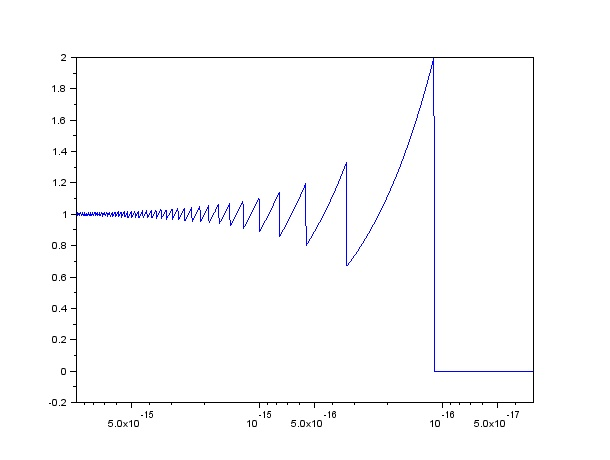
\includegraphics[width=0.8\textwidth]{./cap_aritmetica/pics/cancelamento_0}
  \caption{Gráfico na função do Exemplo~\ref{ex:cancelamento_0}.}
  \label{fig:cancelamento_0}
\end{figure}


\begin{figure}
  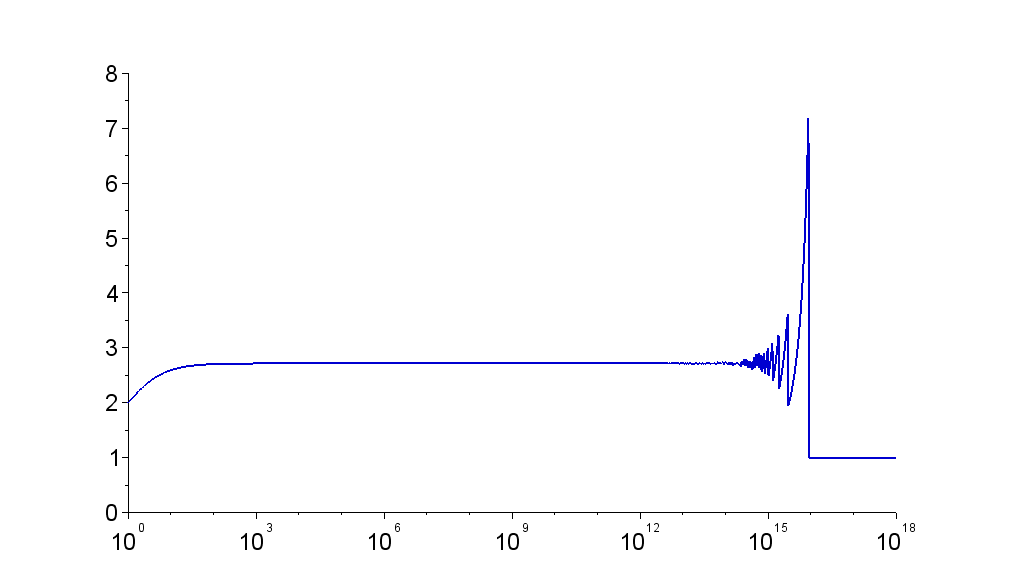
\includegraphics[width=0.8\textwidth]{./cap_aritmetica/pics/cancelamento_euler}
  \label{fig:cancelamento_euler}
  \caption{Gráfico de $\left(1+\frac{1}{n}\right)^n$ em função de $n$ em escala linear-logarítmica variando de $10^0$ até $10^{18}$. Veja o Exemplo~\ref{ex:cancelamento_euler}.}
\end{figure}

\begin{ex}\label{ex:cancelamento_euler} Neste exemplo, estamos interessados em compreender mais detalhadamente o comportamento da expressão
\begin{equation}
  \label{def_lim}\left(1+\frac{1}{n}\right)^n
\end{equation}
quando $n$ é um número grande ao computá-la em sistemas de numeral de ponto flutuante com acurácia finita.
Um resultado bem conhecido do cálculo nos diz que o limite de \eqref{def_lim} quando $n$ tende a infinito é o número de Euler:
\begin{equation}\label{lim}
  \lim_{n\to \infty}\left(1+\frac{1}{n}\right)^n=e= 2,718281828459...
\end{equation}

Sabemos também que a sequência produzida por \eqref{def_lim} é crescente, isto é:
\begin{equation} \left(1+\frac{1}{1}\right)^1< \left(1+\frac{1}{2}\right)^2< \left(1+\frac{1}{3}\right)^3 < \cdots  \end{equation}

No entanto, quando calculamos essa expressão no \verb+Julia+, nos defrontamos com o seguinte resultado:
\begin{center}
\begin{tabular}{|c|c|c|c|c|}\hline &&&&\\[-0.3cm]
$n$ & $\left(1+\frac{1}{n}\right)^n$&$~~~~$&$n$ & $\left(1+\frac{1}{n}\right)^n$\\ &&&&\\[-0.3cm]\hline\\[-0.3cm]
$1$ & $2,0000000000000$ && $10^{2}$ & $2,7048138294215$ \\
$2$ & $2,2500000000000$ && $10^{4}$ & $2,7181459268249$ \\
$3$ & $2,3703703703704$ && $10^{6}$ & $2,7182804690957$ \\
$4$ & $2,4414062500000$ && $10^{8}$ & $2,7182817983391$ \\
$5$ & $2,4883200000000$ && $10^{10}$ & $2,7182820532348$ \\
$6$ & $2,5216263717421$ && $10^{12}$ & $2,7185234960372$ \\
$7$ & $2,5464996970407$ && $10^{14}$ & $2,7161100340870$ \\
$8$ & $2,5657845139503$ && $10^{16}$ & $1,0000000000000$ \\
$9$ & $2,5811747917132$ && $10^{18}$ & $1,0000000000000$ \\
$10$ & $2,5937424601000$ && $10^{20}$ & $1,0000000000000$ \\\hline
\end{tabular}
\end{center}

Podemos resumir esses dados no gráfico de $\left(1+\frac{1}{n}\right)^n$ em função de $n$, veja a Figura~\ref{fig:cancelamento_euler}.

Observe que quando $n$ se torna grande, da ordem de $10^{15}$, o gráfico da função deixa de ser crescente e apresenta oscilações.  Observe também que a expressão se torna identicamente igual a $1$ depois de um certo limiar. Tais fenômenos não são intrínsecos da função $f(n)=(1+1/n)^n$, mas \emph{\uline{oriundas de erros de arredondamento}}, isto é, são resultados numéricos espúrios. A fim de pôr o comportamento numérico de tal expressão, apresentamos abaixo o gráfico da mesma função, porém restrito à região entre $10^{14}$ e $10^{16}$.

Para compreendermos melhor por que existe um limiar $N$ que, quando atingido torna a expressão do exemplo acima identicamente igual a $1$, observamos a sequência de operações realizadas pelo computador:
\begin{equation}\label{seq_oper}
n~\to ~1/n ~\to ~1+1/n ~\to ~(1+1/n)^n
\end{equation}
Devido ao limite de precisão da representação de números em ponto flutuante, existe um menor número representável que é maior do que 1. Este número é $1 + $\verb+eps+, onde \verb+eps+ é chamado de \emph{épsilon de máquina} e é o menor número que somado a 1 produz um resultado superior a 1 no sistema de numeração usado. O épsilon de máquina no sistema de numeração \emph{double} vale aproximadamente $2,22\times 10^{-16}$.

No \verb+GNU Octave+, o épsilon de máquina é a constante \verb+eps+. Observe que:
\begin{verbatim}
>> printf('%1.25f\n', 1+eps)
1.0000000000000002220446049
\end{verbatim}

Quando somamos a $1$ um número positivo inferior ao épsilon de máquina, obtemos o número 1. Dessa forma, o resultado obtido pela operação de ponto flutuante $1+n$ para $0<n<2,22 \times 10^{-16}$ é 1.

Portanto, quando realizamos a sequência de operações dada em \eqref{seq_oper}, toda informação contida no número $n$ é perdida na soma com $1$ quando $1/n$ é menor que o épsilon de máquina, o que ocorre quando $n>5\times 10^{15}$. Assim, $(1+1/n)$ é aproximado para $1$ e a última operação se resume a $1^n$, o que é igual a $1$ mesmo quando $n$ é grande.

Um erro comum é acreditar que o perda de significância se deve ao fato de $1/n$ ser muito pequeno para ser representado e é aproximando para $0$. Isto é falso, o sistema de ponto de flutuante permite representar números de magnitude muito inferior ao épsilon de máquina. O problema surge da limitação no tamanho da mantissa. Observe como a seguinte sequência de operações não perde significância para números positivos x muito menores que o épsilon de máquina:
\begin{equation}\label{seq_oper2}
n ~\to ~1/n ~\to ~1/(1/n)
\end{equation}
compare o desempenho numérico desta sequência de operações para valores pequenos de $n$ com o da seguinte sequência:
\begin{equation}\label{seq_oper3}
n ~\to ~1+n ~\to ~(1+n)-1.
\end{equation}
Finalmente, notamos que quando tentamos calcular $\left(1+\frac{1}{n}\right)^n$ para $n$ grande, existe perda de significância no cálculo de $1+1/n$.

Para entendermos isso melhor, vejamos o que acontece no \verb+GNU Octave+ quando $n=7\times 10^{13}$:
\begin{verbatim}
>> format('long')
>> n=7e13
n =  70000000000000
>> 1/n
ans =    1.42857142857143e-14
>> y=1+1/n
y =  1.00000000000001
\end{verbatim}
Observe a perda de informação ao deslocar a mantissa de $1/n$. Para evidenciar o fenômenos, observamos o que acontece quando tentamos recalcular $n$ subtraindo $1$ de $1+1/n$ e invertendo o resultado:
\begin{verbatim}
>> y-1
ans =    1.42108547152020e-14
>> 1/(y-1)
ans =  70368744177664
\end{verbatim}
\end{ex}

\begin{ex}[Analogia da balança] Observe a seguinte comparação interessante que pode ser feita para ilustrar os sistemas de numeração com ponto fixo e flutuante: o sistema de ponto fixo é como uma balança cujas marcas estão igualmente espaçadas; o sistema de ponto flutuante é como uma balança cuja distância entre as marcas é proporcional à massa medida. Assim, podemos ter uma balança de ponto fixo cujas marcas estão sempre distanciadas de $100$g ($100$g, $200$g, $300$g, ..., $1$kg, $1,1$kg,...) e outra balança de ponto flutuante cujas marcas estão distanciadas sempre de aproximadamente um décimo do valor lido ($100$g, $110$g, $121$g, $133$g, ..., $1$kg, $1,1$kg, $1,21$kg, ...) A balança de ponto fixo apresenta uma resolução baixa para pequenas medidas, porém uma resolução alta para grandes medidas. A balança de ponto flutuante distribui a resolução de forma proporcional ao longo da escala.

Seguindo nesta analogia, o fenômeno de perda de significância pode ser interpretado como a seguir: imagine que você deseje obter o peso de um gato (aproximadamente $4$kg). Dois processos estão disponíveis: colocar o gato diretamente na balança ou medir seu peso com o gato e, depois, sem o gato. Na balança de ponto flutuante, a incerteza associada à medida do peso do gato (sozinho) é aproximadamente $10\%$ de $4$kg, isto é, $400$g. Já a incerteza associada à medida da uma pessoa (aproximadamente $70$kg) com o gato é de $10\%$ do peso total, isto é, aproximadamente $7$kg. Esta incerteza é da mesma ordem de grandeza da medida a ser realizada, tornado o processo impossível de ser realizado, já que teríamos uma incerteza da ordem de $14$kg (devido à dupla medição) sobre uma grandeza de $4$kg.
\end{ex}

\subsection*{Exercícios resolvidos}

\begin{exeresol} Deseja-se medir a concentração de dois diferentes oxidantes no ar. Três sensores eletroquímicos estão disponíveis para a medida e apresentam a seguintes respostas:
\begin{equation} v_1= 270 [A] +  30 [B],~~~ v_2= 140 [A] +  20 [B] ~~ \text{e}~~ v_3= 15 [A] +  200 [B] \end{equation}
as tensões $v_1$, $v_2$ e $v_3$ são dadas em $mV$ e as concentrações em $milimol/l$.
\begin{enumerate}[a)]
\item Encontre uma expressão para os valores de $[A]$ e $[B]$ em termos de $v_1$ e $v_2$ e, depois, em termos de $v_1$ e $v_3$. Dica:
Se $ad\neq bc$, então a matriz $A$ dada por
\begin{equation} A=\begin{bmatrix}a&b\\c&d\end{bmatrix} \end{equation}
é inversível e sua inversa é dada por
\begin{equation} A^{-1}= \frac{1}{ad-bc} \left[\begin{array}{cc}d&-b\\-c&a\end{array}\right]. \end{equation}

\item Sabendo que incerteza relativa associada às sensibilidades dos sensores 1 e 2 é de $2\%$ e que a incerteza relativa associada às sensibilidades do sensor 3 é $10\%$, verifique a incerteza associada à medida feita com o par $1-2$ e o par $1-3$. Use $[A]=[B]=10milimol/l$. Dica: Você deve diferenciar as grandezas $[A]$ e $[B]$ em relação aos valores das tensões.
\end{enumerate}
\end{exeresol}
\begin{resol}
Em ambos casos, temos a seguinte estrutura:
\begin{equation}
\begin{bmatrix}
S_{11}& S_{12}\\
S_{21}& S_{22}
\end{bmatrix}
\begin{bmatrix}
\left[ A\right]\\
\left[ B\right]
\end{bmatrix}
=
\begin{bmatrix}
v_1\\
v_2
\end{bmatrix}
\end{equation}
De forma que
\begin{equation}
\begin{bmatrix}
\left[ A\right]\\
\left[ B\right]
\end{bmatrix}
=\begin{bmatrix}
S_{11}& S_{12}\\
S_{21}& S_{22}
\end{bmatrix}^{-1}
\begin{bmatrix}
v_1\\
v_2
\end{bmatrix}
= \frac{1}{S_{11}S_{22}-S_{12}S_{21}}
\begin{bmatrix}
S_{22}& -S_{12}\\
-S_{21}& S_{11}
\end{bmatrix}
\begin{bmatrix}
v_1\\
v_2
\end{bmatrix}
\end{equation}
Portanto
\begin{eqnarray}
[ A ]&=&\frac{S_{22}v_1-S_{12}v_2}{S_{11}S_{22}-S_{12}S_{21}}\\
\left[ {B} \right]&=&\frac{-S_{21}v_1+S_{11}v_2}{S_{11}S_{22}-S_{12}S_{21}}
\end{eqnarray}

Usando derivação logarítmica, temos

\begin{eqnarray}
\frac{1}{[ A ]}\frac{\partial [ A ]}{\partial S_{11}}&=&-\frac{S_{22}}{S_{11}S_{22}-S_{12}S_{21}}\\
\frac{1}{[ A ]}\frac{\partial [ A ]}{\partial S_{12}}&=&-\frac{v_2}{S_{22}v_1-S_{12}v_2}+\frac{S_{21}}{S_{11}S_{22}-S_{12}S_{21}}\\
&=&-\frac{[A]}{\left[B\right]}\cdot \frac{S_{22}}{S_{11}S_{22}-S_{12}S_{21}}\\
\frac{1}{[ A ]}\frac{\partial [ A ]}{\partial S_{21}}&=&\frac{S_{12}}{S_{11}S_{22}-S_{12}S_{21}}\\
\frac{1}{[ A ]}\frac{\partial [ A ]}{\partial S_{22}}&=&\frac{v_1}{S_{22}v_1-S_{12}v_2}-\frac{S_{11}}{S_{11}S_{22}-S_{12}S_{21}}\\
&=&\frac{[A]}{\left[B\right]}\cdot \frac{S_{12}}{S_{11}S_{22}-S_{12}S_{21}}
\end{eqnarray}
e
\begin{eqnarray}
\frac{1}{\left[ B \right]}\frac{\partial \left[ B \right]}{\partial S_{11}}&=&\frac{v_2}{-S_{21}v_1+S_{11}v_2}-\frac{S_{22}}{S_{11}S_{22}-S_{12}S_{21}}\\
&=&\frac{\left[B\right]}{[A]} \frac{S_{21}}{S_{11}S_{22}-S_{12}S_{21}}\\
\frac{1}{\left[ B \right]}\frac{\partial \left[ B \right]}{\partial S_{12}}&=&\frac{S_{21}}{S_{11}S_{22}-S_{12}S_{21}}\\
\frac{1}{\left[ B \right]}\frac{\partial \left[ B \right]}{\partial S_{21}}&=&-\frac{v_1}{-S_{21}v_1+S_{11}v_2}+\frac{S_{21}}{S_{11}S_{22}-S_{12}S_{21}}\\
&=&-\frac{\left[B\right]}{[A]}\frac{S_{11}}{S_{11}S_{22}-S_{12}S_{21}}\\
\frac{1}{\left[ B \right]}\frac{\partial \left[ B \right]}{\partial S_{22}}&=&-\frac{S_{11}}{S_{11}S_{22}-S_{12}S_{21}}\\
\end{eqnarray}

E o erro associado às medidas pode ser aproximado por
\begin{eqnarray}
\frac{1}{[A]}\delta_{[A]}&=&\left|\frac{1}{[ A ]}\frac{\partial [ A ]}{\partial S_{11}}\right| \delta_{S_{11}}+\left|\frac{1}{[ A ]}\frac{\partial [ A ]}{\partial S_{12}}\right| \delta_{S_{12}}\\
&+&\left|\frac{1}{[ A ]}\frac{\partial [ A ]}{\partial S_{21}}\right| \delta_{S_{21}}+\left|\frac{1}{[ A ]}\frac{\partial [ A ]}{\partial S_{22}}\right| \delta_{S_{22}}\\
&=&\frac{1}{\left|\det{S}\right|}\left[S_{22}\delta_{S_{11}}+\frac{[A]}{\left[B\right]}S_{22}\delta_{S_{12}}+S_{12}\delta_{S_{21}}+\frac{[A]}{\left[B\right]}S_{12}\delta_{S_{22}}\right]
\end{eqnarray}
Analogamente, temos:
\begin{eqnarray}
\frac{1}{[B]}\delta_{[B]}&=&\frac{1}{\left|\det{S}\right|}\left[\frac{[B]}{\left[A\right]}S_{21}\delta_{S_{11}}+S_{21}\delta_{S_{11}}+\frac{\left[B\right]}{[A]}S_{11}\delta_{S_{21}}+S_{11}\delta_{S_{22}}\right]
\end{eqnarray}
onde não se indicou $|S_{ij}|$ nem $|[.]|$ pois são todos positivos.


Fazemos agora a aplicação numérica:\\
{\bf Caso do par 1-2:}
\begin{equation} \det{S}=\left|\begin{matrix}270&30\\140&20\end{matrix}\right|=1200 \end{equation}
\begin{eqnarray}
\frac{1}{[A]}\delta_{[A]}
&=&\frac{1}{1200}\left[20\times 270\times 2\%+20\times 30\times 2\%\right.\\
&\ & \qquad +\left.30\times 140\times 2\%+30\times 20\times 2\%\right]\\&=&\frac{216}{1200}=0.18=18\%\\
\frac{1}{[B]}\delta_{[B]}
&=&\frac{1}{1200}\left[140\times 270\times 2\%+140\times 30\times 2\%\right.\\
&\ & \qquad +\left.270\times 140\times 2\%+270\times 20\times 2\%\right]\\&=&\frac{426}{1200}=0.355=35.5\%
\end{eqnarray}

{\bf Caso do par 1-3:}
\begin{equation} \det{S}=\left|\begin{array}{cc}270&30\\15&200\end{array}\right|=53550 \end{equation}
\begin{eqnarray}
\frac{1}{[A]}\delta_{[A]}
&=&\frac{1}{53550}\left[200\times 270\times 2\%+200\times 30\times 2\%\right.\\
&\ & \qquad +\left.30\times 15\times 10\%+30\times 200\times 10\%\right]\\&=&\frac{1804,6}{52550}\approx 0.0337=3.37\%\\
\frac{1}{[B]}\delta_{[B]}
&=&\frac{1}{53550}\left[15\times 270\times 2\%+15\times 30\times 2\%\right.\\
&\ & \qquad +\left.270\times 15\times 10\%+270\times 200\times 10\%\right]\\&=&	\frac{5895}{53550}\approx   0.11=11\%
\end{eqnarray}
Conclusão, apesar de o sensor $3$ apresentar uma incerteza cinco vezes maior na sensibilidade, a escolha do sensor $3$ para fazer par ao sensor $1$ parece mais adequada.
\end{resol}


\subsection*{Exercícios}

\begin{exer} Considere as expressões:
  \begin{equation}
    \frac{\exp(1/\mu)}{1+\exp(1/\mu)}
  \end{equation}
e
\begin{equation}
  \frac{1}{\exp(-1/\mu)+1}
\end{equation}
com $\mu>0$. Verifique que elas são idênticas como funções reais. Teste no computador cada uma delas para $\mu=0,1$, $\mu=0,01$ e $\mu=0,001$. Qual dessas expressões é mais adequada quando $\mu$ é um número pequeno? Por quê?
\end{exer}
\begin{resp}
  Quando $\mu$ é pequeno, $e^{1/\mu}$ é um número grande. A primeira expressão produz um ''overflow'' (número maior que o máximo representável) quando $\mu$ é pequeno. A segunda expressão, no entanto, reproduz o limite $1$ quando $\mu\to 0+$.
\end{resp}

\begin{exer} Encontre expressões alternativas para calcular o valor das seguintes funções quando $x$ é próximo de zero.
\begin{enumerate}[a)]
\item $f(x)=\frac{1-\cos(x)}{x^2}$
\item $g(x)=\sqrt{1+x}-1$
\item $h(x)=\sqrt{x+10^6}-10^3$
\item $i(x)=\sqrt{1+e^{x}}-\sqrt{2}$ ~~~~~~ Dica: Faça $y=e^{x}-1$
\end{enumerate}
\end{exer}
\begin{resp}
    a)~$\frac{1}{2}+\frac{x^2}{4!}+O(x^4)$; b)~$x/2+O(x^2)$; c)~$5\cdot 10^{-4}x+O(x^2)$; d)~$\frac{\sqrt{2}}{4}y+O(y^{2})=\frac{\sqrt{2}}{4}x+O(x^2)$
\end{resp}

\begin{exer} Use uma identidade trigonométrica adequada para mostrar que:
  \begin{equation}
    \frac{1-\cos(x)}{x^2}= \frac{1}{2} \left(\frac{\sin(x/2)}{x/2}\right)^2.
  \end{equation}
Analise o desempenho destas duas expressões no computador quando $x$ vale $10^{-5}$, $10^{-6}$, $10^{-7}$, $10^{-8}$, $10^{-9}$, $10^{-200}$ e $0$. Discuta o resultado.
\emph{Dica:} Para $|x|<10^{-5}$, $f(x)$ pode ser aproximada por $1/2-x^2/24$ com erro de truncamento inferior a $10^{-22}$.
\end{exer}
\begin{resp}
 A expressão da direita se comporta melhor devido à retirada do cancelamento catastrófico em $x$ em torno de $0$.
\end{resp}


%\begin{exer} Considere a expressão
%\begin{equation}
%f(x)=\frac{1-\cos(x)}{x^2}
% %\end{equation}
%para $x$ pequeno. Verifique que
%\begin{equation}
%\lim_{x\to 0}f(x)=0,5
%\end{equation}
%Depois calcule no \verb+Scilab+ $f(x)$ para $x=10^{-5}$, $x=10^{-6}$, $x=10^{-7}$, $x=10^{-8}$, $x=10^{-9}$ e $x=10^{-10}$. Finalmente, faça uma %aproximação analítica que elimine o efeito catastrófico.
%\end{exer}
%%Redundante


\begin{exer} Reescreva as expressões:
  \begin{equation} \sqrt{e^{2x}+1}-e^x \qquad\text{e}\qquad \sqrt{e^{2x}+x^2}-e^x  \end{equation}
  de modo que seja possível calcular seus valores para $x=100$ utilizando a aritmética de ponto flutuante ("Double") no computador.
\end{exer}
\begin{resp}
 Possíveis soluções são:
 \begin{eqnarray}
  \sqrt{e^{2x}+1}-e^x &=& \sqrt{e^{2x}+1}-e^x \cdot \frac{\sqrt{e^{2x}+1}+e^x }{\sqrt{e^{2x}+1}+e^x }\\
&=&  \frac{e^{2x}+1-e^{2x} }{\sqrt{e^{2x}+1}+e^x }= \frac{1}{\sqrt{e^{2x}+1}+e^x }
 \end{eqnarray}
e, de forma análoga:
 \begin{eqnarray}
  \sqrt{e^{2x}+x^2}-e^x = \frac{x^2}{\sqrt{e^{2x}+x^2}+e^x}.
 \end{eqnarray}
\end{resp}


\begin{exer} Na teoria da relatividade restrita, a energia cinética de uma partícula e sua velocidade se relacionam pela seguinte fórmula:
  \begin{equation}
    E=mc^2\left(\frac{1}{\sqrt{1-(v/c)^2}}-1\right),
  \end{equation}
onde $E$ é a energia cinética da partícula, $m$ é a massa de repouso, $v$ o módulo da velocidade e $c$ a velocidade da luz no vácuo dada por $c=299792458 m/s$. Considere que a massa de repouso $m=9,10938291\times 10^{-31} kg$ do elétron seja conhecida com erro relativo de $10^{-9}$. Qual é o valor da energia e o erro relativo associado a essa grandeza quando $v=0,1 c$, $v=0,5 c$, $v=0,99c$ e $v=0,999c$ sendo que a incerteza relativa na medida da velocidade é $10^{-5}$?
\end{exer}
\begin{resp}
    $4,12451228\times 10^{-16}$~J; $0,002\%$; $0,26654956\times 10^{-14}$~J; $0,002\%$; $4,98497440\times 10^{-13}$~J; $0,057\%$; $1,74927914\times 10^{-12}$~J; $0,522\%$.
\end{resp}

%\end{document}

%Este trabalho está licenciado sob a Licença Creative Commons Atribuição-CompartilhaIgual 3.0 Não Adaptada. Para ver uma cópia desta licença, visite https://creativecommons.org/licenses/by-sa/3.0/ ou envie uma carta para Creative Commons, PO Box 1866, Mountain View, CA 94042, USA.

%\documentclass[main.tex]{subfiles}
%\begin{document}

\chapter{Solução de equações de uma variável}\index{equações!de uma variável}\label{cap:equacao1d}

Neste capítulo, construiremos aproximações numéricas para a solução de \emph{equações algébricas em uma única variável real}. Observamos que obter uma solução para uma dada equação é equivalente a encontrar um \emph{zero de uma função real}\index{função!zero de}\index{função!raiz de} apropriada. Com isso, iniciamos este capítulo discutindo condições de existência e unicidade de raízes de funções de uma variável real. Então, apresentamos o \emph{método da bisseção}\index{método da bisseção} como uma primeira abordagem numérica para a solução de tais equações.

Em seguida, exploramos outra abordagem via \emph{iteração do ponto fixo}\index{iteração do ponto fixo}. Desta, obtemos o \emph{método de Newton}\footnote{Sir Isaac Newton, 1642 - 1727, matemático e físico inglês.}\index{método de Newton}, para o qual estudamos aplicações e critérios de convergência. Por fim, apresentamos o \emph{método das secantes}\index{método das secantes} como uma das possíveis variações do método de Newton.

%%%%%%%%%%%%%%%%%%%%
% python
%%%%%%%%%%%%%%%%%%%%
\ifispython
Ao longo do capítulo, apresentamos algumas computações com \verb+Python+. Nestas, assumiremos o que os seguintes módulos estão carregados:
\begin{verbatim}
>>> import numpy as np
>>> import matplotlib.pyplot as plt
>>> import scipy as sp
>>> from scipy import optimize
\end{verbatim}
A segunda instrução carrega a biblioteca de computação científica \href{http://www.numpy.org/}{numpy} e a terceira carrega a biblioteca gráfica \href{https://matplotlib.org/}{matplotlib}.
\fi

\section{Existência e unicidade}\index{função!}\index{função!zero}

O \emph{teorema de Bolzano}\footnote{Bernhard Placidus Johann Gonzal Nepomuk Bolzano, 1781 - 1848, matemático do Reino da Boêmia.}\index{teorema de!Bolzano} nos fornece condições suficientes para a existência do zero de uma função. Este é uma aplicação direta do \emph{teorema do valor intermediário}\index{teorema do valor intermediário}.

\begin{teo}[Teorema de Bolzano]\label{teo:teorema_de_Bolzano}
  Se $f:[a, b]\to\mathbb{R}$, $y = f(x)$, é uma função contínua tal que $f(a)\cdot f(b) < 0$\footnote{Esta condição é equivalente a dizer que a função troca de sinal no intervalo.}, então existe $x^*\in (a, b)$ tal que $f(x^*) = 0$.
\end{teo}
\begin{proof}
  O resultado é uma consequência imediata do teorema do valor intermediário que estabelece que dada uma função contínua $f:[a, b]\to\mathbb{R}$, $y = f(x)$, tal que $f(a) < f(b)$ (ou $f(b) < f(a)$), então para qualquer $d\in \left(f(a), f(b)\right)$ (ou $k\in \left(f(b), f(a)\right)$) existe $x^*\in (a, b)$ tal que $f(x^*) = k$. Ou seja, nestas notações, se $f(a)\cdot f(b) < 0$, então $f(a) < 0 < f(b)$ (ou $f(b) < 0 < f(a)$). Logo, tomando $k = 0$, temos que existe $x^*\in (a, b)$ tal que $f(x^*) = k = 0$.
\end{proof}

Em outras palavras, se $f(x)$ é uma função contínua em um dado intervalo no qual ela troca de sinal, então ela tem pelo menos um zero neste intervalo (veja a Figura~\ref{fig:teorema_de_Bolzano}).

\begin{figure}
  \centering
  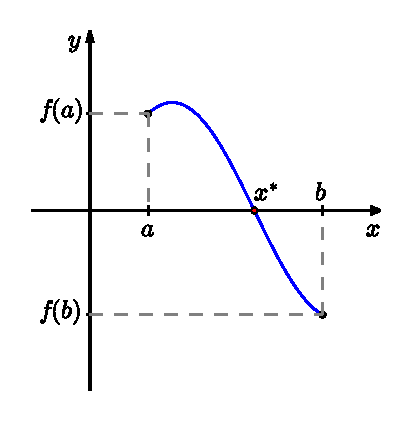
\includegraphics{./cap_equacao1d/pics/teorema_de_Bolzano/teorema_de_Bolzano.eps}
  \caption{Teorema de Bolzano.}
  \label{fig:teorema_de_Bolzano}
\end{figure}

% \begin{teo}[Teorema do Valor Intermediário]
% Se $f:[a,b]\to\mathbb{R}$ é um função contínua e $K$ for um número entre $f(a)$ e $f(b)$, então existe $c\in(a,b)$ para o qual $f(c)=K$.
% \end{teo}

% \begin{figure}[h!]
%   \centering
%   \includegraphics[scale=0.5]{./cap_equacao1d/pics/teorema_do_valor_intermediario/teorema_do_valor_intermediario.eps}
%   \caption{Teorema do valor intermediário}
%   \label{fig:teorema_do_valor_intermediario}
% \end{figure}

% Em particular, se $f(a)>0$ e $f(b)<0$, então $0\in [f(b),f(a)]$ e podemos garantir a existência de $c\in(a,b)$ tal que $f(c)=0$, isto é, existe uma raiz no intervalo $(a,b)$. A mesma afirmação é válida se $f(a)<0$ e $f(b)>0$. Em outras palavras, o teorema do Valor Intermediário afirma que uma função contínua não pode mudar de sinal sem passar por zero.

\begin{ex}\label{ex:teorema_de_Bolzano}
Mostre que existe pelo menos uma solução da equação $e^x=x+2$ no intervalo $(-2,0)$.
\end{ex}
\begin{sol}
Primeiramente, observamos que resolver a equação $e^x = x+2$ é equivalente a resolver $f(x) = 0$ com $f(x)=e^x-x-2$. Agora, como $f(-2)=e^{-2}>0$ e $f(0)=-1<0$, temos do teorema de Bolzano que existe pelo menos um zero de $f(x)$ no intervalo $(-2, 0)$. E, portanto, existe pelo menos uma solução da equação dada no intervalo $(-2, 0)$.

%%%%%%%%%%%%%%%%%%%%
% scilab
%%%%%%%%%%%%%%%%%%%%
\ifisscilab
Podemos usar o \verb+Scilab+ para estudar esta função. Por exemplo, podemos definir a função $f(x)$ e computá-la nos extremos do intervalo dado com os seguintes comandos:
\begin{verbatim}
-->deff('y=f(x)','y=exp(x)-x-2')
-->f(-2),f(0)
 ans  =
    0.1353353
 ans  =
  - 1.
\end{verbatim}
Alternativamente (e com maior precisão), podemos verificar diretamente o sinal da função nos pontos desejados com comando \verb+sign+:
\begin{verbatim}
-->sign(f(-2)),sign(f(0))
 ans  =
    1.
 ans  =
  - 1.
\end{verbatim}
\fi
%%%%%%%%%%%%%%%%%%%%
%%%%%%%%%%%%%%%%%%%%
% octave
%%%%%%%%%%%%%%%%%%%%
\ifisoctave
Podemos usar o \verb+GNU Octave+ para estudar esta função. Por exemplo, podemos definir a função $f(x)$ e computá-la nos extremos do intervalo dado com os seguintes comandos:
\begin{verbatim}
>> f = @(x) exp(x)-x-2
f = f(x) = exp(x)-x-2
>> f(-2),f(0)
ans =  0.13534
ans = -1
\end{verbatim}
Alternativamente (e com maior precisão), podemos verificar diretamente o sinal da função nos pontos desejados com comando \verb+sign+:
\begin{verbatim}
>> sign(f(-2)),sign(f(0))
ans =  1
ans = -1
\end{verbatim}
\fi
%%%%%%%%%%%%%%%%%%%%
%%%%%%%%%%%%%%%%%%%%
% python
%%%%%%%%%%%%%%%%%%%%
\ifispython
Podemos usar \verb+Python+ para estudar esta função. Por exemplo, podemos definir a função $f(x)$ e computá-la nos extremos do intervalo dado com os seguintes comandos:
\begin{verbatim}
>>> def f(x): return np.exp(x)-x-2
...
>>> f(-2),f(0)
(0.13533528323661281, -1.0)
\end{verbatim}
Alternativamente (e com maior precisão), podemos verificar diretamente o sinal da função nos pontos desejados com a função \href{https://docs.scipy.org/doc/numpy/reference/generated/numpy.sign.html?highlight=numpy.sign#numpy.sign}{numpy.sign}:
\begin{verbatim}
>>> np.sign(f(-2)*f(0))
-1.0
\end{verbatim}
\fi
%%%%%%%%%%%%%%%%%%%%
\end{sol}


Quando procuramos aproximações para zeros de funções, é aconselhável isolar cada raiz em um intervalo. Desta forma, gostaríamos de poder garantir a existência e a unicidade da raiz dentro de um dado intervalo. A seguinte proposição nos fornece condições suficientes para tanto.

\begin{prop}\label{prop:existencia_e_unicidade}
Se $f:[a, b]\to\mathbb{R}$ é um função diferenciável, $f(a)\cdot f(b)<0$ e $f'(x)>0$ (ou $f'(x)<0$) para todo $x\in(a, b)$, então existe um único $x^*\in (a, b)$ tal que $f(x^*) = 0$.
\end{prop}

Em outras palavras, para garantirmos que exista um único zero de uma dada função diferenciável em um intervalo, é suficiente que ela troque de sinal e seja monótona neste intervalo.

\begin{ex}
No Exemplo~\ref{ex:teorema_de_Bolzano}, mostramos que existe pelo menos um zero de $f(x) = e^{x}-x-2$ no intervalo $(-2,0)$, pois $f(x)$ é contínua e $f(-2)\cdot f(0) < 0$. Agora, observamos que, além disso, $f'(x)=e^x-1$ e, portanto, $f'(x) < 0$ para todo $x\in(-2,0)$. Logo, da Proposição~\ref{prop:existencia_e_unicidade}, temos garantida a existência de um único zero no intervalo dado.

%%%%%%%%%%%%%%%%%%%%
% scilab
%%%%%%%%%%%%%%%%%%%%
\ifisscilab
Podemos inspecionar o comportamento da função $f(x)= e^x - x - 2$ e de sua derivada fazendo seus gráficos no Scilab. Para tanto, podemos fazer o seguinte teste:
\begin{verbatim}
-->x = linspace(-2,0,50);
-->deff('y = f(x)','y=exp(x)-x-2')  // define f
-->plot(x,f(x));xgrid               // gráfico de f
-->deff('y = fl(x)','y=exp(x)-1')   // a derivada
-->plot(x,fl(x));xgrid              // gráfico de f'
\end{verbatim}
\fi
%%%%%%%%%%%%%%%%%%%%
%%%%%%%%%%%%%%%%%%%%
% octave
%%%%%%%%%%%%%%%%%%%%
\ifisoctave
Podemos inspecionar o comportamento da função $f(x)= e^x - x - 2$ e de sua derivada fazendo seus gráficos no \verb+GNU Octave+. Para tanto, podemos fazer o seguinte teste:
\begin{verbatim}
>> xx = linspace(-2,0,50);
>> f = @(x) exp(x)-x-2  #define f
f = f(x) = exp(x)-x-2
>> plot(xx,f(xx))grid on;hold on #gráfico de f
>> fl = @(x) exp(x)-1  #a derivada
fl = f(x) = exp(x)-1
>> plot(xx,fl(xx)) #gráfico de f'
\end{verbatim}
\fi
%%%%%%%%%%%%%%%%%%%%
%%%%%%%%%%%%%%%%%%%%
% python
%%%%%%%%%%%%%%%%%%%%
\ifispython
Podemos inspecionar o comportamento da função $f(x)= e^x - x - 2$ e de sua derivada fazendo seus gráficos no Python. Para tanto, podemos usar o seguinte código \verb+Python+:
\begin{verbatim}
>>> def f(x): return np.exp(x)-x-2
...
>>> xx = np.linspace(-2,0)
>>> plt.plot(xx,f(xx))
>>> plt.grid(); plt.show()

>>> def fl(x): return np.exp(x)-1
...
>>> plt.plot(xx,fl(xx))
>>> plt.grid(); plt.show()
\end{verbatim}
\fi
%%%%%%%%%%%%%%%%%%%%
\end{ex}

A discussão feita nesta seção, especialmente o teorema de Bolzano, nos fornece os fundamentos para o método da bisseção, o qual discutimos na próxima seção.

\subsection*{Exercícios}
\begin{exer}\label{exer:existencia_sol1}
  Mostre que $\cos x = x$ tem solução no intervalo $[0, \pi/2]$.
\end{exer}
\begin{resp}

  Observamos que a equação é equivalente a $\cos(x) - x = 0$. Tomando, então, $f(x) = \cos(x) - x$, temos que $f(x)$ é contínua em $[0, \pi/2]$, $f(0) = 1$ e $f(\pi/2) = -\pi/2 < 0$. Logo, do teorema de Bolzano~\ref{teo:teorema_de_Bolzano}, concluímos que a equação dada tem pelo menos uma solução no intervalo $(0, \pi/2)$.

\end{resp}

\begin{exer}
  Mostre que $\cos x = x$ tem uma única solução no intervalo $[0, \pi/2]$.
\end{exer}
\begin{resp}

    No Exercício~\ref{exer:existencia_sol1}, mostramos que a função $f(x) = \cos(x) - x$ tem um zero no intervalo $[0, \pi/2]$. Agora, observamos que $f'(x) = -\sen(x) - 1$. Como $0 < \sen x < 1$ para todo $x\in (0, \pi/2)$, temos que $f'(x) < 0$ em $(0, \pi/2)$, isto é, $f(x)$ é monotonicamente decrescente neste intervalo. Logo, da Proposição~\ref{prop:existencia_e_unicidade}, temos que existe um único zero da função neste intervalo.

\end{resp}

\begin{exer} Interprete a equação $\cos(x)=kx$ como o problema de encontrar a intersecção da curva $y=\cos(x)$ com $y=kx$. Encontre o valor positivo $k$ para o qual essa equação admite exatamente duas raízes positivas distintas.
\end{exer}
\begin{resp}

    $k\approx 0,161228$

\end{resp}


\begin{exer}Mostre que a equação:
  \begin{equation}
    \ln(x)+x^3-\frac{1}{x}=10
  \end{equation}
possui uma única solução positiva.
\end{exer}

\begin{exer}\label{exer:teorema_de_Bolzano_exatidao} Use o teorema de Bolzano para mostrar que o erro absoluto ao aproximar o zero da função $f(x)=e^x-x-2$ por $\overline{x}=-1,841$ é menor que $10^{-3}$.
\end{exer}
\begin{resp}

    Escolhendo o intervalo $[a, b] = [-1,841-10^{-3}, -1,841+10^{-3}]$, temos $f(a)\approx 5\times 10^{-4} > 0$ e $f(b)\approx -1,2\times 10^{-3} < 0$, isto é, $f(a)\cdot f(b) < 0$. Então, o teorema de Bolzano nos garante que o zero exato $x^*$ de $f(x)$ está no intervalo $(a, b)$. Logo, da escolha feita, $|-1,841 - x^*| < 10^{-3}$.

\end{resp}

\begin{exer} Mostre que o erro absoluto associado à aproximação $\overline{x} = 1,962$ para a solução exata $x^*$ de:
  \begin{equation}
    e^x+\sin (x) +x = 10
  \end{equation}
é menor que $10^{-4}$.
\end{exer}
\begin{resp}
  Basta aplicar as ideias da solução do Exercício~\ref{exer:teorema_de_Bolzano_exatidao}.
\end{resp}

\begin{exer}\label{existe_unica} Mostre que a equação
  \begin{equation}
    \ln(x)+x-\frac{1}{x}=v
  \end{equation}
possui uma solução para cada $v$ real e que esta solução é única.
\end{exer}

\section{Método da bisseção}\index{método!da bisseção}

O \emph{método da bisseção} explora o fato de que uma função contínua $f:[a, b]\to \mathbb{R}$ com $f(a)\cdot f(b) < 0$ tem um zero no intervalo $(a, b)$ (veja o teorema de Bolzano~\ref{teo:teorema_de_Bolzano}). Assim, a ideia para aproximar o zero de uma tal função $f(x)$ é tomar, como aproximação inicial, o ponto médio do intervalo $[a, b]$, isto é:
\begin{equation}
  x^{(0)} = \frac{(a + b)}{2}.
\end{equation}
Pode ocorrer de $f(x^{(0)}) = 0$ e, neste caso, o zero de $f(x)$ é $x^* = x^{(0)}$. Caso contrário, se $f(a)\cdot f(x^{(0)}) < 0$, então $x^*\in (a, x^{(0)})$. Neste caso, tomamos como nova aproximação do zero de $f(x)$ o ponto médio do intervalo $[a, x^{(0)}]$, isto é, $x^{(1)} = (a + x^{(0)})/2$. No outro caso, temos $f(x^{(0)})\cdot f(b) < 0$ e, então, tomamos $x^{(1)} = (x^{(0)} + b)/2$. Repetimos este procedimento até obtermos a aproximação desejada (veja Figura~\ref{fig:metodo_da_bissecao}).

\begin{figure}
  \centering
  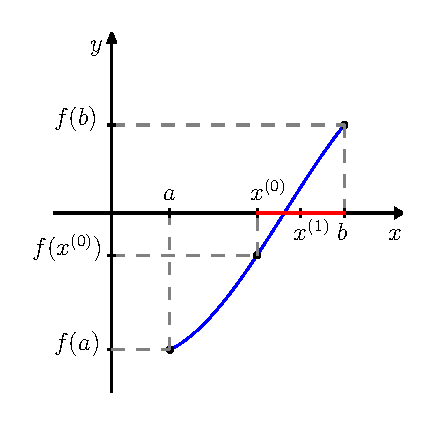
\includegraphics{./cap_equacao1d/pics/metodo_da_bissecao/metodo_da_bissecao.eps}
  \caption{Método da bisseção.}
  \label{fig:metodo_da_bissecao}
\end{figure}

De forma mais precisa, suponha que queiramos calcular uma aproximação com uma certa precisão $TOL$ para um zero $x^*$ de uma dada função contínua $f:[a, b]\to\mathbb{R}$ tal que $f(a)\cdot f(b) < 0$. Iniciamos, tomando $n=0$ e:
\begin{equation}
  a^{(n)} = a,\quad b^{(n)} = b\quad\text{e}\quad x^{(n)} = \frac{a^{(n)} + b^{(n)}}{2}.
\end{equation}
Verificamos o \emph{critério de parada}\index{critério de parada}, isto é, se $f(x^{(n)}) = 0$ ou:
\begin{equation}
  \displaystyle \frac{|b^{(n)} - a^{(n)}|}{2} < TOL,
\end{equation}
então $x^{(n)}$ é a aproximação desejada. Caso contrário, preparamos a próxima iteração $n+1$ da seguinte forma: se $f(a^{(n)})\cdot f(x^{(n)}) < 0$, então definimos $a^{(n+1)} = a^{(n)}$ e $b^{(n+1)} = x^{(n)}$; no outro caso, se $f(x^{(n)})\cdot f(b^{(n)}) < 0$, então definimos $a^{(n+1)} = x^{(n)}$ e $b^{(n+1)} = b^{(n)}$. Trocando $n$ por $n+1$, temos a nova aproximação do zero de $f(x)$ dada por:
\begin{equation}
  x^{(n+1)} = \frac{a^{(n+1)} + b^{(n+1)}}{2}.
\end{equation}
Voltamos a verificar o critério de parada acima e, caso não satisfeito, iteramos novamente. Iteramos até obtermos a aproximação desejada ou o número máximo de iterações ter sido atingido.

\begin{ex}\label{ex:metodo_da_bissecao}Use o método da bisseção para calcular uma solução de $e^x = x + 2$ no intervalo $[-2, 0]$ com precisão $TOL = 10^{-1}$.
\end{ex}
\begin{sol}
  Primeiramente, observamos que resolver a equação dada é equivalente a calcular o zero de $f(x) = e^x - x - 2$. Além disso, temos $f(-2)\cdot f(0) < 0$. Desta forma, podemos iniciar o método da bisseção tomando o intervalo inicial $[a^{(0)}, b^{(0)}] = [-2, 0]$ e:
  \begin{equation}
    x^{(0)} = \frac{a^{(0)} + b^{(0)}}{2} = -1.
  \end{equation}
  Apresentamos as iterações na Tabela~\ref{tab:metodo_da_bissecao}. Observamos que a precisão $TOL = 10^{-1}$ foi obtida aproximando o zero de $f(x)$ por $x^{(4)} = -1,8125$.
  \begin{table}
    \centering
    \caption{Iteração do método da bisseção para o Exemplo~\ref{ex:metodo_da_bissecao}.}
    \label{tab:metodo_da_bissecao}
    \begin{tabular}{l|ccc|c|c}\hline
      $n$ & $a^{(n)}$ & $b^{(n)}$ & $x^{(n)}$ & $f(a^{(n)})f(x^{(n)})$ & $\displaystyle \frac{|b^{(n)}-a^{(n)}|}{2}$\\\hline
      $0$ & $-2$ & $0$ & $-1$ & $< 0$ & $1$\\
      $1$ & $-2$ & $-1$ & $-1,5$ & $<0$ & $0,5$\\
      $2$ & $-2$ & $-1,5$ & $-1,75$ & $<0$ & $0,25$\\
      $3$ & $-2$ & $-1,75$ & $-1,875$ & $>0$ & $0,125$\\
      $4$ & $-1,875$ & $-1,75$ & $-1,8125$ & $<0$ & $0,0625$\\\hline
    \end{tabular}
  \end{table}

%%%%%%%%%%%%%%%%%%%%
% scilab
%%%%%%%%%%%%%%%%%%%%
\ifisscilab
Usando o \verb+Scilab+ neste exemplo, temos:
\begin{verbatim}
-->deff('y = f(x)','y = exp(x) - x - 2')
-->a=-2, b=0, x=(a+b)/2, TOL = (b-a)/2, sign(f(a)*f(x))
-->b=x, x=(a+b)/2, TOL = (b-a)/2, sign(f(a)*f(x))
\end{verbatim}
  e, assim, sucessivamente. Veja o código completo na Seção~\ref{subsec:codigo_bissecao}.
\fi
%%%%%%%%%%%%%%%%%%%%
%%%%%%%%%%%%%%%%%%%%
% octave
%%%%%%%%%%%%%%%%%%%%
\ifisoctave
Usando o \verb+GNU Octave+ neste exemplo, temos:
\begin{verbatim}
>> f = @(x) exp(x) - x - 2
f = f(x) = exp(x) - x - 2
>> a=-2, b=0, x=(a+b)/2, TOL = (b-a)/2, sign(f(a)*f(x))
a = -2
b = 0
x = -1
TOL =  1
ans = -1
>> b=x, x=(a+b)/2, TOL = (b-a)/2, sign(f(a)*f(x))
b = -1
x = -1.5000
TOL =  0.50000
ans = -1
\end{verbatim}
e, assim, sucessivamente. Veja o código completo na Seção~\ref{subsec:codigo_bissecao}.
\fi
%%%%%%%%%%%%%%%%%%%%
%%%%%%%%%%%%%%%%%%%%
% python
%%%%%%%%%%%%%%%%%%%%
\ifispython
Usando \verb+Python+ neste exemplos, temos:
\begin{verbatim}
>>> def f(x): return np.exp(x) - x - 2
...
>>> a=-2; b=0; x = (a+b)/2; [a,b,x]
[-2, 0, -1.0]
>>> [(b-a)/2, np.sign(f(a)*f(x))]
[1.0, -1.0]
>>> b=x; x=(a+b)/2; [a,b,x]
[-2, -1.0, -1.5]
>>> [(b-a)/2, np.sign(f(a)*f(x))]
\end{verbatim}
e, assim, sucessivamente. Veja o código completo na Seção~\ref{subsec:codigo_bissecao}.
\fi
%%%%%%%%%%%%%%%%%%%%
\end{sol}

Vamos agora discutir sobre a \emph{convergência} do método da bisseção, que é garantida pelo Teorema~\ref{teo:convergencia_bissecao}.

\begin{teo}[Convergência do método da bisseção]\label{teo:convergencia_bissecao} Sejam $f:[a, b]\to \mathbb{R}$ uma função contínua tal que $f(a)\cdot f(b) < 0$ e $x^*$ o único zero de $f(x)$ no intervalo $(a, b)$. Então, a sequência $\{x^{(n)}\}_{n \geq 0}$ do método da bisseção satisfaz:
  \begin{equation}
    |x^{(n)} - x^{*}| < \frac{b - a}{2^{n+1}},\quad\forall n\geq 0.
  \end{equation}
Em particular, $x^{(n)}\to x^*$ quando $n\to\infty$.
\end{teo}
\begin{proof}
 Notemos que, a cada iteração, a distância entre a aproximação $x^{(n)}$ e o zero $x^*$ da função é menor ou igual que a metade do tamanho do intervalo $[a^{(n)}, b^{(n)}]$ (veja Figura~\ref{fig:metodo_da_bissecao}), isto é:
\begin{equation}
  |x^{(n)}-x^*| \leq \frac{b^{(n)}-a^{(n)}}{2}.
\end{equation}
Por construção do método, temos $[a^{(n)}, b^{(n)}]\subset [a^{(n-1)}, b^{(n-1)}]$ quando $n \geq 1$ e:
\begin{equation}
  b^{(n)} - a^{(n)} = \frac{b^{(n-1)}-a^{(n-1)}}{2}.
\end{equation}
Desta forma:
\begin{equation}
  |x^{(n)}-x^*|  \leq \frac{b^{(n)}-a^{(n)}}{2} = \frac{b^{(n-1)}-a^{(n-1)}}{2^2} = \cdots = \frac{b^{(0)}-a^{(0)}}{2^{n+1}},\quad \forall n\geq 1.
\end{equation}
Logo, vemos que:
\begin{equation}
  |x^{(n)}-x^*|  \leq \frac{b-a}{2^{n+1}},\quad \forall n\geq 0.
\end{equation}
\end{proof}

Observamos que a hipótese de que $f(x)$ tenha um único zero no intervalo não é realmente necessária. Se a função tiver mais de um zero no intervalo inicial, as iterações ainda convergem para um dos zeros. Veja o Exercício~\ref{exer:raizes_multiplas}.

\begin{obs}
  O Teorema~\ref{teo:convergencia_bissecao} nos fornece uma estimativa para a convergência do método da bisseção. Aproximadamente, temos:
  \begin{equation}
    |x^{(n+1)} - x^*| \lesssim \frac{1}{2}|x^{(n)} - x^*|.
  \end{equation}
Isto nos leva a concluir que o método da bisseção tem \emph{taxa de convergência}\index{Método da bisseção!taxa de convergência} linear.
\end{obs}

\begin{ex}No Exemplo~\ref{ex:metodo_da_bissecao}, depois de escolhida a aproximação inicial $x^{(0)} = -1 \in [a, b] = [-2, 0]$, precisamos de $4$ iterações do método da bisseção para computar uma aproximação com precisão de $10^{-1}$ do zero de $f(x) = e^x - x - 2$. Poderíamos ter estimado o número de iterações \emph{a priori}, pois, como vimos acima:
  \begin{equation}
    |x^{(n)}-x^*|\leq \frac{b-a}{2^{n+1}},\quad n\geq 0.
  \end{equation}
Logo, temos:
\begin{eqnarray}
  |x^{(n)} - x^*| &<& \frac{b - a}{2^{n+1}} = \frac{2}{2^{n+1}}\\
  &=& 2^{-n} < 10^{-1} \Rightarrow  n > -\log_2 10^{-1} \approx 3,32.
\end{eqnarray}
Isto está de acordo com o experimento numérico realizado naquele exemplo.
\end{ex}

O método da bisseção tem a boa propriedade de garantia de convergência, bem como de fornecer uma simples estimativa do erro na aproximação calculada. Entretanto, a taxa de convergência linear é superada por outros métodos. A construção de tais métodos está, normalmente, associada à iteração do ponto fixo, a qual exploramos na próxima seção.

%%%%%%%%%%%%%%%%%%%%
% scilab
%%%%%%%%%%%%%%%%%%%%
\ifisscilab
\subsection{Código Scilab: método da bisseção}\label{subsec:codigo_bissecao}

O seguinte código é uma implementação no \verb+Scilab+ do algoritmo da bisseção. As variáveis de entrada são:
\begin{itemize}
\item \verb+f+ - função objetivo
\item \verb+a+ - extremo esquerdo do intervalo de inspeção $[a, b]$
\item \verb+b+ - extremo direito do intervalo de inspeção $[a, b]$
\item \verb+TOL+ - tolerância para o erro absoluto (critério de parada)
\item \verb+N+ - número máximo de iterações depois da aproximação inicial
\end{itemize}
A variável de saída é:
\begin{itemize}
\item \verb+p+ - aproximação de uma raiz $x^*$ de \verb+f+, satisfazendo $|p - x^*|< TOL$ ou $f(p) = 0$.
\end{itemize}

\verbatiminput{./cap_equacao1d/codes/scilab/metodo_da_bissecao/bissecao.sci}
\fi
%%%%%%%%%%%%%%%%%%%%
%%%%%%%%%%%%%%%%%%%%
% octave
%%%%%%%%%%%%%%%%%%%%
\ifisoctave
\subsection{Código GNU Octave: método da bisseção}\label{subsec:codigo_bissecao}

O seguinte código é uma implementação no \verb+GNU Octave+ do algoritmo da bisseção. As variáveis de entrada são:
\begin{itemize}
\item \verb+f+ - função objetivo
\item \verb+a+ - extremo esquerdo do intervalo de inspeção $[a, b]$
\item \verb+b+ - extremo direito do intervalo de inspeção $[a, b]$
\item \verb+TOL+ - tolerância para o erro absoluto (critério de parada)
\item \verb+N+ - número máximo de iterações depois da aproximação inicial
\end{itemize}
A variável de saída é:
\begin{itemize}
\item \verb+p+ - aproximação de uma raiz $x^*$ de \verb+f+, satisfazendo $|p - x^*|< TOL$ ou $f(p) = 0$.
\end{itemize}

\verbatiminput{./cap_equacao1d/codes/octave/metodo_da_bissecao/bissecao.m}
\fi
%%%%%%%%%%%%%%%%%%%%
%%%%%%%%%%%%%%%%%%%%
% python
%%%%%%%%%%%%%%%%%%%%
\ifispython
\subsection{Código Python: método da bisseção}\label{subsec:codigo_bissecao}

O seguinte código é uma implementação em \verb+Python+ do algoritmo da bisseção. As variáveis de entrada são:
\begin{itemize}
\item \verb+f+ - função objetivo
\item \verb+a+ - extremo esquerdo do intervalo de inspeção $[a, b]$
\item \verb+b+ - extremo direito do intervalo de inspeção $[a, b]$
\item \verb+TOL+ - tolerância para o erro absoluto (critério de parada)
\item \verb+N+ - número máximo de iterações depois da aproximação inicial
\end{itemize}
A variável de saída é:
\begin{itemize}
\item \verb+p+ - aproximação de uma raiz $x^*$ de \verb+f+, satisfazendo $|p - x^*|< TOL$ ou $f(p) = 0$.
\end{itemize}

\verbatiminput{./cap_equacao1d/codes/python/metodo_da_bissecao/bissecao.py}
\fi
%%%%%%%%%%%%%%%%%%%%

\subsection*{Exercícios}

\begin{exer}Considere a equação $\sqrt{x}=\cos(x)$. Use o método da bisseção com intervalo inicial $[a, b] = [0, 1]$ e $x^{(1)} = (a+b)/2$ para calcular a aproximação $x^{(4)}$ da solução desta equação.
\end{exer}
\begin{resp}
  0,6875
\end{resp}

\begin{exer} Trace o gráfico e isole as três primeiras raízes positivas da função:
  \begin{equation}
    f(x)=5\sin(x^2)-\exp\left({\frac{x}{10}}\right)
  \end{equation}
em intervalos de comprimento $0,1$. Então, use o método da bisseção para obter aproximações dos zeros desta função com precisão de $10^{-5}$.
\end{exer}
\begin{resp}
  Intervalo $(0,4, 0,5)$, zero $0,45931$. Intervalo $(1,7, 1,8)$, zero $1,7036$. Intervalo $(2,5, 2,6)$, zero $2,5582$.
\end{resp}

\begin{exer}\label{exer:raizes_multiplas}
  O polinômio $p(x) = -4 + 8x - 5x^2 + x^3$ tem raízes $x_1=1$ e $x_2=x_3=2$ no intervalo $[1/2, 3]$.
  \begin{itemize}
  \item[a)] Se o método da bisseção for usando com o intervalo inicial $[1/2, 3]$, para qual raiz as iterações convergem?
  \item[b)] É possível usar o método da bisseção para a raiz $x=2$? Justifique sua resposta.
  \end{itemize}
\end{exer}
\begin{resp}
  a) $x_1=1$. b) Dica: como $x_2=2$ é raiz dupla, tem-se que $p'(x_2) = 0$.
\end{resp}

\begin{exer}\label{prob_raiz_dupla} O polinômio $f(x)=x^4-4x^2+4$ possui raízes duplas em $\sqrt{2}$ e $-\sqrt{2}$. O método da bisseção pode ser aplicado a $f$? Explique.
\end{exer}


\begin{exer} Mostre que a equação do Problema~\ref{existe_unica} possui uma solução no intervalo $[1, v+1]$ para todo $v$ positivo. Dica: defina $f(x)=\ln(x)+x-\frac{1}{x}-v$  e considere a seguinte estimativa:
  \begin{equation}
    f(v+1)=f(1)+\int_1^{v+1}f'(x)dx\geq -v+\int_1^{v+1}dx=0.
  \end{equation}
Use esta estimativa para iniciar o método de bisseção e obtenha o valor da raiz com pelo menos 6 algarismos significativos para $v=1, 2, 3, 4$ e $5$.
\end{exer}
\begin{resp}
    $1,390054$; $1,8913954$; $2,4895673$; $3,1641544$; $3,8965468$
\end{resp}

\begin{exer}(Estática) Considere o seguinte problema físico: uma plataforma está fixa a uma parede através de uma dobradiça cujo momento é dado por:
  \begin{equation}
    \tau=k\theta,
  \end{equation}
onde $\theta$ é ângulo da plataforma com a horizontal e $k$ é uma constante positiva. A plataforma é feita de material homogêneo, seu peso é $P$ e sua largura é $l$. Modele a relação entre o ângulo $\theta$ e o peso $P$ próprio da plataforma. Encontre o valor de $\theta$ quando $l=1~\mbox{m}$, $P=200~\mbox{N}$, $k=50~\mbox{Nm}/\mbox{rad}$, sabendo que o sistema está em equilíbrio. Use o método da bisseção e expresse o resultado com 4 algarismos significativos.
\end{exer}
\begin{resp}
    $k\theta=\frac{lP}{2}\cos(\theta)$ com $\theta\in (0, \pi/2)$; $1,030$.
\end{resp}


\begin{exer} Considere a equação de Lambert dada por:
  \begin{equation}
    xe^x= t,
  \end{equation}
onde $t$ é um número real positivo. Mostre que esta equação possui uma única solução $x^*$ que pertence ao intervalo $[0, t]$. Usando esta estimativa como intervalo inicial, quantos passos são necessário para obter o valor numérico de $x^*$ com erro absoluto inferior a $10^{-6}$ quando $t=1$, $t=10$ e $t=100$ através do método da bisseção? Obtenha esses valores.
\end{exer}
\begin{resp}
    $19$; $23$; $26$; $0,567143$; $1,745528$; $3,385630$
\end{resp}

\begin{exer}(Eletrônica)\label{prob_diodo} O desenho abaixo mostra um circuito não linear envolvendo uma fonte de tensão constante, um diodo retificador e um resistor. Sabendo que a relação entre a corrente ($I_d)$ e a tensão ($v_d$) no diodo é dada pela seguinte expressão:
  \begin{equation}
    I_d=I_R\left(\exp\left(\frac{v_d}{v_t}\right)-1\right),
  \end{equation}
onde $I_R$ é a corrente de condução reversa e $v_t$, a tensão térmica dada por $v_t=\frac{kT}{q}$ com $k$, a constante de Boltzmann, $T$ a temperatura de operação e $q$, a carga do elétron. Aqui  $I_R=1pA=10^{-12}~\mbox{A}$, $T=300~\mbox{K}$. Escreva o problema como uma equação na incógnita $v_d$ e, usando o método da bisseção, resolva este problema com 3 algarismos significativos para os seguintes casos:
\end{exer}
\begin{minipage}[l]{0.6\linewidth}
\begin{itemize}
\item[a)] $V=30~\mbox{V}$ e $R=1~\mbox{k}\Omega$.
\item[b)] $V=3~\mbox{V}$ e $R=1~\mbox{k}\Omega$.
\item[c)] $V=3~\mbox{V}$ e $R=10~\mbox{k}\Omega$.
\item[d)] $V=300~\mbox{mV}$ e $R=1~\mbox{k}\Omega$.
\item[e)] $V=-300~\mbox{mV}$ e $R=1~\mbox{k}\Omega$.
\item[f)] $V=-30~\mbox{V}$ e $R=1~\mbox{k}\Omega$.
\item[g)] $V=-30~\mbox{V}$ e $R=10~\mbox{k}\Omega$.
\end{itemize}\end{minipage}\begin{minipage}[c]{0.4\linewidth}
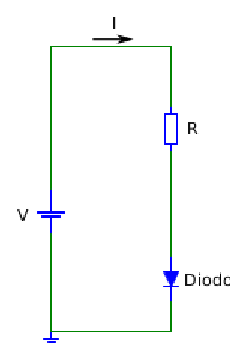
\includegraphics[width=0.9\textwidth]{./cap_equacao1d/pics/circuito_diodo.eps}
\end{minipage}\\
Dica: $V=RI_d+v_d$.
\begin{resp}
    a) $0,623$; b) $0,559$; c) $0,500$; d) $0,300$; e) $-0,3$; f) $-30$; g) $-30$
\end{resp}

\begin{exer}(Propagação de erros) Obtenha os valores de $I_d$ no Problema~\ref{prob_diodo}. Lembre que existem duas expressões disponíveis:
  \begin{equation}
    I_d=I_R\left(\exp\left(\frac{v_d}{v_t}\right)-1\right)
  \end{equation}
e
\begin{equation}
  I_d=\frac{v-v_d}{R}
\end{equation}
Faça o estudo da propagação do erro e decida qual a melhor expressão em cada caso.
\end{exer}
\begin{resp}
  a) $0,0294$; b) $2.44e-3$; c) $2.50e-4$; d) $1.09\cdot 10^{-7}$; e) $- 10^{-12}$; f) $-10^{-12}$; g) $- 10^{-12}$
\end{resp}

\section{Iteração de ponto fixo}\index{iteração do ponto fixo}

Nesta seção, discutimos a abordagem da \emph{iteração do ponto fixo} para a solução numérica de equações de uma variável real. Observamos que sempre podemos reescrever uma equação da forma $f(x) = 0$ (problema de encontrar os zeros de uma função) em uma equação equivalente na forma $g(x) = x$ (\emph{problema de ponto fixo}\index{problema de!ponto fixo}). Um ponto $x = x^*$ tal que $g(x^*) = x^*$ é chamado de \emph{ponto fixo}\index{ponto fixo} da função $g(x)$. Geometricamente, um ponto fixo de uma função é um ponto de interseção entre a reta $y = x$ com o gráfico da função $g(x)$ (veja Figura~\ref{fig:defn_ponto_fixo}).

\begin{figure}[h]
  \centering
  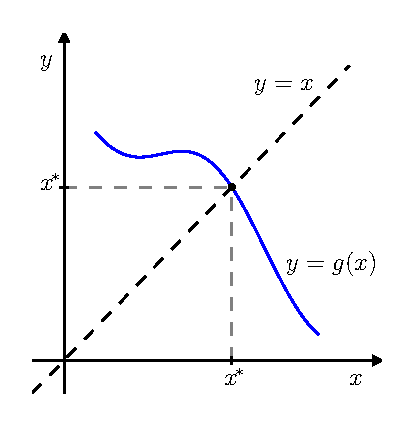
\includegraphics{./cap_equacao1d/pics/defn_ponto_fixo/defn_ponto_fixo.eps}
  \caption{Ponto fixo $g(x^*) = x^*$.}
  \label{fig:defn_ponto_fixo}
\end{figure}

\begin{ex}\label{ex:ponto_fixo_1}
  Resolver a equação $e^x = x + 2$ é equivalente a resolver $f(x) = 0$, com $f(x) = e^x - x - 2$. Estes são equivalentes a resolver $g(x) = x$, com $g(x) = e^x - 2$, isto é:
  \begin{equation}
    e^x = x + 2 \Leftrightarrow e^x - x - 2 = 0 \Leftrightarrow e^x - 2 = x
  \end{equation}
\end{ex}

Dada uma função $g(x)$, a \emph{iteração do ponto fixo} consiste em computar a seguinte sequência recursiva:
\begin{equation}
  x^{(n+1)} = g(x^{(n)}), \quad n\geq 1,
\end{equation}
onde $x^{(1)}$ é uma aproximação inicial do ponto fixo.

\begin{ex}[Método babilônico]
O método babilônico\footnote{Heron de Alexandria, 10 d.C. - 70 d.C., matemático grego.} é de uma iteração de ponto fixo para extrair a raiz quadrada de um número positivo $A$, isto é, resolver a equação $x^2 = A$.

Seja $r>0$ uma aproximação para $\sqrt{A}$. Temos três possibilidades:
\begin{itemize}
\item $r>\sqrt{A} \Longrightarrow \frac{A}{r}<\sqrt{A} \Longrightarrow \sqrt{A}\in \left(\frac{A}{r}, r\right);$
\item $r=\sqrt{A} \Longrightarrow \frac{A}{r}=\sqrt{A};$
\item $r<\sqrt{A} \Longrightarrow \frac{A}{r}>\sqrt{A} \Longrightarrow \sqrt{A}\in \left(r, \frac{A}{r}\right).$
\end{itemize}
Ou seja, $\sqrt{A}$ sempre está no intervalo entre $r$ e $\frac{A}{r}$, no qual podemos buscar uma nova aproximação como, por exemplo, pelo ponto médio:
\begin{equation} x=\frac{r+\frac{A}{r}}{2}. \end{equation}

Aplicando esse método repetidas vezes, podemos construir a iteração (de ponto fixo):
\begin{eqnarray}
x^{(1)}&=&r \\
x^{(n+1)}&=&\frac{x^{(n)}}{2}+\frac{A}{2x^{(n)}}, \quad n=1,2,3,...
\end{eqnarray}

Por exemplo, para obter uma aproximação para $\sqrt{5}$, podemos iniciar com a aproximação inicial $r=2$ e $A=5$. Então, tomamos $x^{(1)} = 2$ e daí seguem as aproximações:
\begin{eqnarray}
x^{(2)}&=&\frac{2}{2}+\frac{2,5}{2} = 2,25\\
x^{(3)}&=&\frac{2,25}{2}+\frac{2,5}{2,25}= 2,2361111  \\
x^{(4)}&=&\frac{2,2361111}{2}+\frac{2,5}{2,2361111}= 2,236068  \\
x^{(5)}&=&\frac{2,236068}{2}+\frac{2,5}{2,236068}= 2,236068
\end{eqnarray}
\end{ex}

% \begin{ex}
% Para obter uma aproximação para $\sqrt{10}$, podemos iniciar com $r=1$ e $A=10$.

% Assim
% \begin{align*}
% x^{(1)}=1
% \end{align*}
% e a partir de
% \begin{align*}
% x^{(n+1)}&=\frac{x^{(n)}}{2}+\frac{5}{x^{(n)}}
% \end{align*}
% obtemos
% \begin{align*}
% x^{(2)}&=\frac{1}{2}+\frac{5}{1}=0,5+5=5,5\\
% x^{(3)}&=\frac{5,5}{2}+\frac{5}{5,5}=3,6590909 \\
% x^{(4)}&=\frac{3,6590909}{2}+\frac{5}{3,6590909}=3,1960051   \\
% x^{(5)}&=\frac{3,1960051}{2}+\frac{5}{3,1960051}=3,1624556  \\
% x^{(6)}&=\frac{3,1624556}{2}+\frac{5}{3,1624556}=3,1622777  \\
% x^{(7)}&=\frac{3,1622777}{2}+\frac{5}{3,1622777}=3,1622777
% \end{align*}
% \end{ex}

O método babilônico sugere que a iteração do ponto fixo pode ser uma abordagem eficiente para a solução de equações. Ficam, entretanto, as seguintes perguntas:
\begin{enumerate}
\item Será que a iteração do ponto fixo é convergente?
\item Caso seja convergente, será que o limite da sequência produzida, isto é, $x^* := \lim_{n\to \infty }x^{(n)}$ é um ponto fixo?
\item Caso seja convergente, qual é a taxa de convergência?
\end{enumerate}

A segunda pergunta é a mais fácil de ser respondida. No caso de $g(x)$ ser contínua, se $x^{(n)}\to x^*\in\Dom(g)$, então:
\begin{equation}
  x^* = \lim_{n\to\infty} x^{(n)} = \lim_{n\to\infty} g(x^{(n-1)}) = g\left(\lim_{n\to\infty} x^{(n-1)}\right) = g(x^*).
\end{equation}

% Supondo que o limite de $x_n$ exista, basta substituir $x^*$ na iteração:
% \begin{eqnarray}
% \lim_{n \to \infty }x^{(n+1)}&=&\lim_{n \to \infty }\frac{x^{(n)}}{2}+\lim_{n \to \infty }\frac{A}{2x^{(n)}}\\
% x^*&=&\frac{x^*}{2}+\frac{A}{2x^*}\\
% \frac{x^*}{2}&=&\frac{A}{2x^*}\\
% {x^*}&=&\frac{A}{x^*}\\
% {(x^*)}^2&=&{A}\\
% x^*&=&\sqrt{A}
% \end{eqnarray}
% Portanto, sempre que esse método converge, temos a garantia de que o limite é $\sqrt{A}$. (Independente do valor inicial!)

% De fato, podemos provar que o método é convergente para qualquer valor inicial positivo $x$. E, ainda, que a convergência é rápida (ainda precisamos definir isso).

Antes de respondermos as outras perguntas acima, vejamos mais um exemplo.

\begin{ex}\label{ex:ponto_fixo_2}
  Considere o problema de encontrar o zero da função $f(x) = xe^x - 10$. Uma maneira geral de construir um problema de ponto fixo equivalente é o seguinte:
  \begin{equation}
    f(x) = 0 \Rightarrow \alpha f(x) = 0 \Rightarrow x - \alpha f(x) = x,
  \end{equation}
para qualquer parâmetro $\alpha\neq 0$. Consideremos, então, as seguintes duas funções:
\begin{equation}
  g_1(x) = x - 0,5f(x)\quad\text{e}\quad g_2(x) = x - 0,05f(x).
\end{equation}
Notamos que o ponto fixo destas duas funções coincide com o zero de $f(x)$. Construindo as iterações do ponto fixo:
\begin{equation}
  x_1^{(n+1)} = g_1(x_1^{(n)})\quad\text{e}\quad x_2^{(n+1)} = g_2(x_2^{(n)}),
\end{equation}
tomando $x_1^{(1)} = x_2^{(1)} = 1,7$, obtemos os resultados apresentados na Tabela~\ref{tab:ponto_fixo_2}. Observamos que, enquanto, a iteração do ponto fixo com a função $g_1(x)$ ($\alpha = 0,5$) parece divergir, a iteração com a função $g_2(x)$ ($\alpha = 0,05$) parece convergir.

\begin{table}
  \centering
  \caption{Iterações do ponto fixo para o Exemplo~\ref{ex:ponto_fixo_2}.}\label{tab:ponto_fixo_2}
  \begin{tabular}{c|rr}\hline
    $n$ & $x_1^{(n)}$ & $x_2^{(n)}$ \\\hline
    $1$ & $1,700$ & $1,700$\\
    $2$ & $2,047$ & $1,735$\\
    $3$ & $-0,8812$ & $1,743$ \\
    $4$ & $4,3013$ & $1,746$\\
    $5$ & $-149,4$ & $1,746$\\\hline
  \end{tabular}
\end{table}

%%%%%%%%%%%%%%%%%%%%
% scilab
%%%%%%%%%%%%%%%%%%%%
\ifisscilab
No \verb+Scilab+, podemos computar as iterações do ponto fixo $x^{(n+1)} = g_1(x^{(n)})$ com o seguinte código:
\begin{verbatim}
--> deff('y = f(x)', 'y = x*exp(x)-10')
--> deff('y = g1(x)', 'y = x - 0.5*f(x)')
--> x = 1.7;
--> x = g1(x)
x =
    2.0471
--> x = g1(x)
x =
   -0.88119
\end{verbatim}
e, assim, sucessivamente. Itere com a função $g_2(x)$ e verifique a convergência!
\fi
%%%%%%%%%%%%%%%%%%%%
%%%%%%%%%%%%%%%%%%%%
% octave
%%%%%%%%%%%%%%%%%%%%
\ifisoctave
No \verb+GNU Octave+, podemos computar as iterações do ponto fixo $x^{(n+1)} = g_1(x^{(n)})$ com o seguinte código:
\begin{verbatim}
>> f = @(x) x*exp(x)-10
f = f(x) = x*exp(x)-10
>> g1 = @(x) x - 0.5*f(x)
g1 = f(x) = x - 0.5*f(x)
>> x = 1.7;
>> x = g1(x)
x =  2.0471
>> x = g1(x)
x = -0.88119
\end{verbatim}
e, assim, sucessivamente. Itere com a função $g_2(x)$ e verifique a convergência!
\fi
%%%%%%%%%%%%%%%%%%%%
%%%%%%%%%%%%%%%%%%%%
% python
%%%%%%%%%%%%%%%%%%%%
\ifispython
Em \verb+Python+, podemos computar as iterações do ponto fixo $x^{(n+1)} = g_1(x^{(n)})$ com o seguinte código:
\begin{verbatim}
>>> def f(x): return x*np.exp(x)-10
...
>>> def g1(x): return x-0.5*f(x)
...
>>> x=1.7
>>> x=g1(x);x
2.0471447170318804
>>> x=g1(x);x
-0.88119413893725618
\end{verbatim}
e, assim, sucessivamente. Itere com a função $g_2(x)$ e verifique a convergência!
\fi
%%%%%%%%%%%%%%%%%%%%
\end{ex}
% Para responder essas perguntas, devemos formalizar o conceito de ponto fixo. Antes disso, analisemos mais um exemplo:



% Note que queríamos resolver a equação $f(x)=x e^x-10=0$. Ao invés disso, transformamos essa equação em uma equação de iteração do tipo
%   \begin{equation} x^{(n+1)}=g(x^{(n)}) \end{equation}
% e iteramos até encontrar $p$ tal que $g(p)=p$.



% \subsection{O método do ponto fixo}\index{ponto fixo}

% \begin{defn}
%   Dizemos que  $p$ é um \emph{ponto fixo} de uma função $g$ se $g(p)=p$.
% \end{defn}

A fim de estudarmos a convergência da iteração do ponto fixo, apresentamos o teorema do ponto fixo.

\subsection{Teorema do ponto fixo}\index{Teorema do!ponto fixo}

O teorema do ponto fixo nos fornece condições suficientes para a existência e unicidade do ponto fixo, bem como para a convergência das iterações do método.

\begin{defn}
 Uma \emph{contração}\index{contração} é uma função real $g:[a, b]\to [a, b]$ tal que:
 \begin{equation}
   |g(x)-g(y)|\leq \beta |x-y|,\quad 0\leq \beta < 1.
 \end{equation}
\end{defn}

\begin{obs}Seja $g:[a, b]\to [a, b]$, y=g(x).
  \begin{itemize}
  \item Se $g(x)$ é uma contração, então $g(x)$ é uma função contínua.
  \item Se $|g'(x)| < k$, $0 < k < 1$, para todo $x\in [a, b]$, então $g(x)$ é uma contração.
  \end{itemize}
\end{obs}

\begin{teo}[Teorema do ponto fixo]
 Se $g:[a,b]\to [a,b]$ é uma contração, então existe um único ponto $x^*\in [a, b]$ tal que $g(x^*)= x^*$, isto é, $x^*$ é ponto fixo de $g(x)$. Além disso, a sequência $\{x^{(n)}\}_{n\in\mathbb{N}}$ dada por:
 \begin{equation}
   x^{(n+1)}=g(x^{(n)})
 \end{equation}
converge para $x^*$ para qualquer $x^{(1)}\in [a, b]$.
\end{teo}
\begin{proof}
Começamos demonstrando que existe pelo menos um ponto fixo. Para tal definimos a função $f(x)=x-g(x)$ e observamos que:
\begin{equation}
  f(a)=a-g(a)\leq a-a=0
\end{equation}
e
\begin{equation}
  f(b)=b-g(b)\geq b-b=0
\end{equation}
Se $f(a)=a$ ou $f(b)=b$, então o ponto fixo existe. Caso contrário, as desigualdades são estritas e a $f(x)$ muda de sinal no intervalo.  Como esta função é contínua, pelo teorema de Bolzano~\ref{teo:teorema_de_Bolzano}, existe um ponto $x^*$ no intervalo $(a, b)$ tal que $f(x^*)=0$, ou seja, $g(x^*)=x^*$. Isto mostra a existência.

Para provar que o ponto fixo é único, observamos que se $x^*$ e $x^{**}$ são pontos fixos, eles devem ser iguais, pois:
\begin{equation}
  |x^*-x^{**}| = |g(x^{*})-g(x^{**})| \leq \beta |x^*-x^{**}|.
\end{equation}
A desigualdade $|x^*-x^{**}|\leq \beta |x^*-x^{**}|$ com $0\leq \beta<1$ implica $|x^*-x^{**}|=0$.

Para demonstrar a convergência da sequência, observamos que:
\begin{equation}
  |x^{(n+1)}-x^*| = |g(x^{(n)})-x^*| = |g(x^{(n)})-g(x^*)| \leq \beta |x^{(n)}-x^*|.
\end{equation}
Daí, temos:
\begin{equation}
  |x^{(n)}-x^*|\leq  \beta |x^{(n-1)}-x^*|\leq \beta^2 |x^{(n-2)}-x^*|\leq \cdots \leq \beta^{n}|x^{(0)}-x^*|.
\end{equation}
Portanto, como $0\leq\beta<1$, temos:
\begin{equation}
  \lim_{n\to\infty}|x^{(n)}-x^*|=0,
\end{equation}
ou seja, $x^{(n)}\to x^*$ quando $n\to\infty$.
\end{proof}

\begin{obs}
  Do teorema do ponto fixo, temos que se $g(x)$ é uma contração com constante $0\leq \beta < 1$, então:
  \begin{equation}
    |x^{(n+1)}-x^*| \leq \beta |x^{(n)}-x^*|,\quad n\geq 1.
  \end{equation}
Isto é, as iterações do ponto fixo têm taxa de convergência linear\index{iteração do ponto fixo!taxa de convergência}.
\end{obs}

\begin{ex}\label{ex:ponto_fixo_3}
Mostre que o teorema do ponto fixo se aplica a função $g(x) = \cos(x)$ no intervalo $[1/2, 1]$, isto é, a iteração de ponto fixo converge para a solução da equação $\cos x = x$. Então, calcule as iterações do ponto fixo com aproximação inicial $x^{(1)} = 0,7$, estime o erro absoluto da aproximação e verifique a taxa de convergência.
\end{ex}
\begin{sol}
  Basta mostrarmos que:
  \begin{enumerate}
  \item[a)] $g\left([1/2,1]\right) \subseteq [1/2,1]$;
  \item[b)] $|g'(x)|<\beta, \quad 0<\beta<1,\quad \forall x\in [1/2,1]$.
  \end{enumerate}

Para provar a), observamos que $g(x)$ é decrescente no intervalo, pelo que temos:
\begin{equation}
  0,54<\cos(1)\leq \cos(x)\leq \cos(1/2)<0,88
\end{equation}
Como $[0,54,~0,88]\subseteq [0,5,~1]$, temos o item a).

Para provar o item b), observamos que:
\begin{equation}
  g'(x) = -\sin(x).
\end{equation}
Da mesma forma, temos a estimativa:
\begin{equation}
  -0,85<-\sin(1) \leq -\sin(x)\leq -\sin(1/2)<-0,47.
\end{equation}
Assim, $|g'(x)|<0,85$ e temos a desigualdade com $\beta=0,85<1$.

\begin{table}
  \centering
  \begin{tabular}{l|ccc}\hline
   $n$ & $x^{(n)}$ & $\epsilon_n := |x^{(n)} - x^*|$ \\\hline
   $1$ & $0,70000$ & $3,9\E-02$ \\
   $2$ & $0,76484$ & $2,6\E-02$ \\
   $3$ & $0,72149$ & $1,8\E-02$ \\
   $4$ & $0,75082$ & $1,2\E-02$ \\
   $5$ & $0,73113$ & $8,0\E-03$ \\
   $6$ & $0,74442$ & $5,3\E-03$ \\
   $7$ & $0,73548$ & $3,6\E-03$ \\\hline
  \end{tabular}
  \caption{Iteração do ponto fixo para o Exemplo~\ref{ex:ponto_fixo_3}.}
  \label{tab:ponto_fixo_3}
\end{table}


A Tabela~\ref{tab:ponto_fixo_3} apresenta o comportamento numérico da iteração do ponto fixo:
\begin{eqnarray}
x^{(1)} &=& 0,7\\
x^{(n+1)} &=& \cos(x^{(n)}),\quad n\geq 1.
\end{eqnarray}
Para estimar o erro, consideramos $x^* = 0,7390851605$. A Figura~\ref{fig:ex_ponto_fixo_3} mostrar o decaimento do erro $\epsilon_n = |x^{(n)} - x^*|$ comparado com a taxa de convergência linear com $\beta = 0,85$.

\begin{figure}
  \centering
  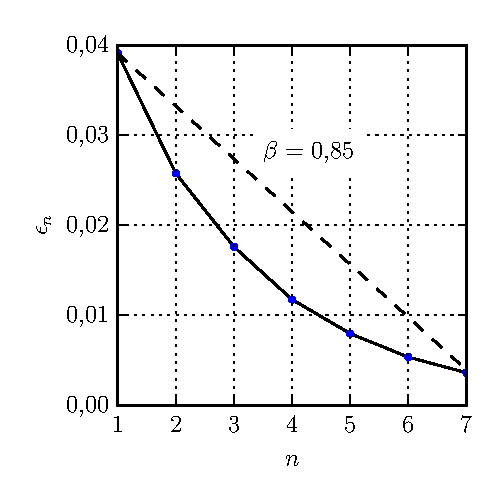
\includegraphics{./cap_equacao1d/pics/ex_ponto_fixo_3/ex_ponto_fixo_3}
  \caption{Decaimento do erro $\epsilon_n = |x^{(n)}-x^*|$ da iteração do ponto fixo estudada no Exemplo~\ref{ex:ponto_fixo_3}.}
  \label{fig:ex_ponto_fixo_3}
\end{figure}


%%%%%%%%%%%%%%%%%%%%
% scilab
%%%%%%%%%%%%%%%%%%%%
\ifisscilab
No \verb+Scilab+, podemos computar estas iterações e o erro absoluto com o seguinte código:
\begin{verbatim}
//est. da solucao
deff('y = f(x)', 'y = cos(x)-x')
xe = fsolve(0.7, f)

#funcao do pto. fixo
deff('y = g(x)', 'y = cos(x)')

#aprox. inicial
x0 = 0.7
eps = abs(x0-xe)
disp([x0, eps])

for i=2:7
  x = g(x0)
  eps = abs(x-xe)
  disp([x, eps])
  x0 = x
end
\end{verbatim}
\fi
%%%%%%%%%%%%%%%%%%%%
%%%%%%%%%%%%%%%%%%%%
% octave
%%%%%%%%%%%%%%%%%%%%
\ifisoctave
No \verb+GNU Octave+, podemos computar estas iterações e o erro absoluto com o seguinte código:
\begin{verbatim}
#est. da solucao
f = @(x) cos(x)-x;
xe = fsolve(f, 0.7);

#funcao do pto. fixo
g = @(x) cos(x);

#aprox. inicial
x0 = 0.7;
eps = abs(x0-xe);
printf("%1.5f %1.1e\n", x0, eps);

for i=2:7
  x = g(x0);
  eps = abs(x-xe);
  printf("%1.5f %1.1e\n", x, eps)
  x0 = x;
endfor
\end{verbatim}
\fi
%%%%%%%%%%%%%%%%%%%%
%%%%%%%%%%%%%%%%%%%%
% python
%%%%%%%%%%%%%%%%%%%%
\ifispython
Em \verb+Python+, podemos computar estas iterações, o erro absoluto com o seguinte código:
\begin{verbatim}
#funcao do pto. fixo
def g(x):
    return np.cos(x)

#est. da solucao
xe = sp.optimize.fixed_point(g, 0.7)

#aprox. inicial
x0 = 0.7
eps = np.fabs(x0-xe)
print("x1 =  %.5f, eps =~ %.1e" % (x0, eps))

for i in np.arange(7):
    x = g(x0);
    eps = np.fabs(x-xe);
    print("%s =~ %.5f, eps =~ %.1e" % (('x'+str(i+2)), x, eps))
    x0 = x
\end{verbatim}
\fi
%%%%%%%%%%%%%%%%%%%%
\end{sol}

\subsection{Teste de convergência}
Seja $g:[a,b]\to\mathbb{R}$ uma função $C^0[a,b]$ e $x^*\in(a,b)$ um ponto fixo de $g$. Então $x^*$ é dito estável se existe uma região $(x^*-\delta,x^*+\delta)$ chamada bacia de atração tal que $x^{(n+1)}=g(x^{(n)})$ é convergente sempre que $x^{(0)}\in(x^*-\delta,x^*+\delta)$.

\begin{prop}[Teste de convergência]
 Se $g\in C^1[a,b]$ e  $|g'(x^*)|<1$, então $x^*$ é estável. Se $|g'(x^*)|>1$ é instável e o teste é inconclusivo quando $|g'(x^*)|=1$.
\end{prop}

\begin{figure}[h]
    \centering
        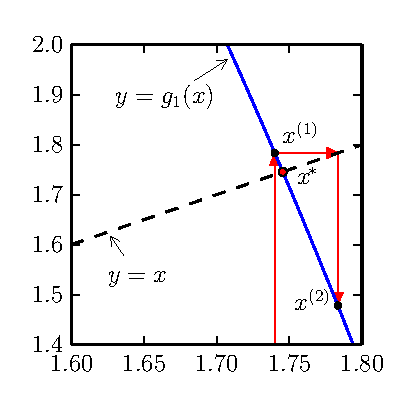
\includegraphics{./cap_equacao1d/pics/ponto_fixo_instavel/ponto_fixo_instavel.eps}
~
        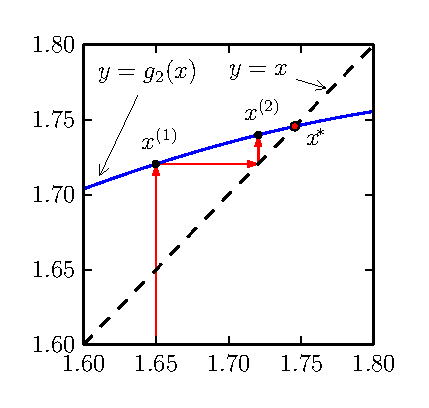
\includegraphics{./cap_equacao1d/pics/ponto_fixo_estavel/ponto_fixo_estavel.eps}
    \caption{Ilustração das iterações do ponto fixo para: (esquerda) $y = g_1(x)$ e (direita) $y = g_2(x)$. Veja Exemplo~\ref{ex:ponto_fixo_4}.} \label{fig:teste_de_convergencia}
\end{figure}

\begin{ex}\label{ex:ponto_fixo_4}
  No Exemplo~\ref{ex:ponto_fixo_2}, observamos que a função $g_1(x)$ nos forneceu uma iteração divergente, enquanto que a função $g_2(x)$ forneceu uma iteração convergente (veja a Figura~\ref{fig:teste_de_convergencia}. Estes comportamentos são explicados pelo teste da convergência. Com efeito, sabemos que o ponto fixo destas funções está no intervalo $[1,6, 1,8]$ e temos:
  \begin{equation}
    |g_1'(x)| = |1 - 0,5(x+1)e^x| > 4,8,\quad\forall x\in [1,6, 1,8],
  \end{equation}
enquanto:
\begin{equation}
  |g_2'(x)| = |1 - 0,05(x+1)e^x| < 0,962,\quad\forall x\in [1,6, 1,8].
\end{equation}
\end{ex}

\subsection{Estabilidade e convergência}\index{iteração do ponto fixo!estabilidade}\index{iteração do ponto fixo!convergência}

A fim de compreendermos melhor os conceitos de estabilidade e convergência, considere uma função $\Phi(x)$ com um ponto fixo $x^*=g(x^*)$ e analisemos o seguinte processo iterativo:
\begin{eqnarray}
x^{(n+1)}&=&g\left(x^{(n)}\right)\\
x^{(0)}&=&x
\end{eqnarray}
Vamos supor que a função $g(x)$ pode ser aproximada por seu polinômio de Taylor em torno do ponto fixo:
\begin{eqnarray}
g(x)&=&g(x^*)+(x-x^*) g'(x^*)+O\left((x-x^*)^2\right)\\
&=&x^*+(x-x^*) g'(x^*)+O\left((x-x^*)^2\right)\\
&\approx& x^*+(x-x^*) g'(x^*)
\end{eqnarray}

Substituindo na relação de recorrência, temos
\begin{equation}
x^{(n+1)}=g\left(x^{(n)}\right)\approx x^*+(x^{(n)}-x^*) g'(x^*)
\end{equation}
Ou seja:
\begin{equation}
\left(x^{(n+1)}-x^*\right)\approx {(x^{(n)}-x^*)} g'(x^*)
\end{equation}
Tomando módulos, temos:
\begin{equation}
\underbrace{\left|x^{(n+1)}-x^*\right|}_{\epsilon_{n+1}}\approx \underbrace{\left|x^{(n)}-x^*\right|}_{\epsilon_n} \left|g'(x^*)\right|,
\end{equation}
onde $\epsilon_n=\left|x^{(n)}-x^*\right|$.

\begin{obs} Da análise acima, concluímos:
\begin{itemize}
\item Se $|g'(x^*)|<1$, então, a distância de $x^{(n)}$ até o ponto fixo $x^*$ está diminuindo a cada passo.
\item Se $|g'(x^*)|>1$, então, a distância de $x^{(n)}$ até o ponto fixo $x^*$ está aumentando a cada passo.
\item Se $|g'(x^*)|=1$, então, nossa aproximação de primeira ordem não é suficiente para compreender o comportamento da sequência.
\end{itemize}
\end{obs}

\subsection{Erro absoluto e tolerância}\index{erros!absoluto}\index{tolerância}

Na prática, quando se aplica uma iteração como esta, não se conhece de antemão o valor do ponto fixo $x^*$. Assim, o erro $\epsilon_n=\left|x^{(n)}-x^*\right|$ precisa ser estimado com base nos valores calculados $x^{(n)}$. Uma abordagem frequente é analisar a evolução da diferença entre dois elementos da sequência:
\begin{equation} \Delta_n=\left|x^{(n+1)}-x^{(n)}\right| \end{equation}

A pergunta natural é: Será que o erro $\epsilon_n=\left|x^{(n)}-x^*\right|$ será pequeno quando  $\Delta_n=\left|x^{(n+1)}-x^{(n)}\right|$ for pequeno?

Para responder a esta pergunta, observamos que
\begin{equation} x^*=\lim_{n\to \infty }x^{(n)} \end{equation}
portanto:
\begin{eqnarray}
x^*-x^{(N)}&=&  \left(x^{(N+1)}-x^{(N)}\right)+\left(x^{(N+2)}-x^{(N+1)}\right)+\left(x^{(N+3)}-x^{(N+2)}\right)+\ldots\\
&=&\sum_{k=0}^\infty \left(x^{(N+k+1)}-x^{(N+k)}\right)
\end{eqnarray}

Usamos também as expressões:
\begin{eqnarray}
x^{(n+1)}&\approx& x^*+(x^{(n)}-x^*) g'(x^*)\\
x^{(n)}&\approx& x^*+(x^{(n-1)}-x^*) g'(x^*)
\end{eqnarray}
Subtraindo uma da outra, temos:
\begin{eqnarray}
x^{(n+1)}-x^{(n)}&\approx& (x^{(n)}-x^{(n-1)}) g'(x^*)
\end{eqnarray}
Portanto:
\begin{eqnarray}
x^{(N+k+1)}-x^{(N+k)}&\approx& (x^{(N+1)}-x^{(N)}) \left(g'(x^*)\right)^{k}
\end{eqnarray}
E temos:
\begin{eqnarray}
x^*-x^{(N)}
&=&\sum_{k=0}^\infty \left(x^{(N+k+1)}-x^{(N+k)}\right)\\
&\approx&\sum_{k=0}^\infty (x^{(N+1)}-x^{(N)}) \left(g'(x^*)\right)^{k}\\
&=&(x^{(N+1)}-x^{(N)}) \frac{1}{1-g'(x^*)}, \quad \left|g'(x^*)\right|<1
\end{eqnarray}
Tomando módulo, temos:
\begin{eqnarray}
\left|x^*-x^{(N)} \right|
&\approx&\left|x^{(N+1)}-x^{(N)}\right| \frac{1}{1-g'(x^*)}\\
\epsilon_N &\approx&  \frac{\Delta_N}{1-g'(x^*)}
\end{eqnarray}

\begin{obs}
Tendo em mente a relação $x^{(n+1)}-x^{(n)}  \approx (x^{(n)}-x^{(n-1)}) g'(x^*)$, concluímos:
\begin{itemize}

\item Quando $g'(x^*)<0$, o esquema é alternante, isto é, o sinal do erro se altera a cada passo.  O erro $\epsilon_N$ pode ser estimado diretamente da diferença $\Delta_N$, pois o denominador $1-g'(x^*)>1$.
\item Quando $0<g'(x^*)<1$, o esquema é monótono e $\frac{1}{1-g'(x^*)}>1$, pelo que o erro $\epsilon_N$ é maior que a diferença $\Delta_N$. A relação será tão mais importante quando mais próximo da unidade for $g'(x^*)$, ou seja, quando mais lenta for a convergência. Para estimar o erro em função da diferença $\Delta_N$, observamos que  $g'(x^*)\approx \frac{x^{(n+1)}-x^{(n)}}{x^{(n)}-x^{(n-1)}}$ e
\begin{equation} \left|g'(x^*)\right|\approx \frac{\Delta_n}{\Delta_{n-1}} \end{equation}
e portanto
\begin{equation} \epsilon_N \approx \frac{\Delta_N}{1-\frac{\Delta_n}{\Delta_{n-1}}}. \end{equation}
\end{itemize}
\end{obs}

\subsection*{Exercícios}

\begin{exer}
  Resolver a equação $e^x = x + 2$ é equivalente a calcular os pontos fixos da função $g(x) = e^x - 2$ (veja o Exemplo~\ref{ex:ponto_fixo_1}). Use a iteração do ponto fixo $x^{(n+1)} = g(x^{n})$ com $x^{(1)} = -1,8$ para obter uma aproximação de uma das soluções da equação dada com $8$ dígitos significativos.
\end{exer}
\begin{resp}
    $-1,8414057$
\end{resp}

\begin{exer}  Mostre que a equação:
  \begin{equation}
    \cos(x)=x
  \end{equation}
possui uma única solução no intervalo $[0, 1]$. Use a iteração do ponto fixo e encontre uma aproximação para esta solução com  4 dígitos significativos.
\end{exer}
\begin{resp}

    $0,7391$

\end{resp}

\begin{exer}
  Mostre que a equação $xe^x = 10$ é equivalente às seguintes equações:
\begin{equation}
  x=\ln\left(\frac{10}{x}\right)\quad\text{e}\quad x=10e^{-x}.
\end{equation}
Destas, considere as seguintes iterações de ponto fixo:
\begin{enumerate}
 \item [a)] $\displaystyle x^{(n+1)}=\ln \left(\frac{10}{x^{(n)}}\right)$
 \item [b)] $\displaystyle x^{(n+1)}=10 e^{-x^{(n)}} $
\end{enumerate}
Tomando $x^{(1)} = 1$, verifique se estas sequências são convergentes.
\end{exer}
\begin{resp}

Tomemos $x^{(1)}=1$ como aproximação inicial para a solução deste problema, iterando a primeira sequência a), obtemos:
\begin{eqnarray}
x^{(1)} &=& 1\\
x^{(2)} &=& \ln\left(\frac{10}{1}\right)=2,3025851\\
x^{(3)} &=& \ln\left(\frac{10}{2,3025851}\right)=1,4685526\\
        &\vdots&\\
x^{(21)}&=& 1,7455151\\
x^{(31)}&=& 1,745528\\
x^{(32)}&=& 1,745528
\end{eqnarray}

Iterando a segunda sequência b), obtemos:
\begin{eqnarray}
x^{(1)}&=&1\\
x^{(2)}&=&10e^{-1}= 3,6787944   \\
x^{(3)}&=&10e^{- 3,6787944 }= 0,2525340     \\
x^{(4)}&=&10e^{-0,2525340}=  7,7682979      \\
x^{(5)}&=&10e^{-7,7682979}=  0,0042293      \\
x^{(6)}&=&10e^{-0,0042293}=  9,9577961
\end{eqnarray}

Este experimento numérico sugere que a iteração a) converge para $1,745528$ e a iteração b) não é convergente.

\end{resp}

\begin{exer} Verifique (analiticamente) que a única solução real da equação:
  \begin{equation}
    xe^x=10
  \end{equation}
é ponto fixo das seguintes funções:
\begin{itemize}
\item[a)] $g(x)=\ln\left(\frac{10}{x}\right)$
\item[b)] $g(x)=x-\frac{xe^{x}-10}{15}$
\item[c)] $g(x)=x-\frac{xe^{x}-10}{10+e^{x}}$
\end{itemize}
Implemente o processo iterativo $x^{(n+1)}=g(x^{(n)})$ para $n\geq 0$ e compare o comportamento. Discuta os resultados com base na teoria estudada.
\end{exer}

\begin{exer} Verifique (analiticamente) que a única solução real da equação:
  \begin{equation}
    \cos(x)=x
  \end{equation}
é ponto fixo das seguintes funções:
\begin{itemize}
\item[a)] $g(x)=\cos(x)$
\item[b)] $g(x)=0,4 x+ 0,6\cos(x)$
\item[c)] $g(x)=x+\frac{\cos(x)-x}{1+\sin(x)}$
\end{itemize}
Implemente o processo iterativo $x^{(n+1)}=g(x^{(n)})$ para $n\geq 0$ e compare o comportamento. Discuta os resultados com base na teoria estudada.
\end{exer}


\begin{exer} Encontre a solução de cada equação com erro absoluto inferior a $10^{-6}$.
  \begin{itemize}
  \item[a)] $e^x=x+2$ no intervalo $(-2,0)$.
  \item[b)] $x^3+5x^2-12=0$ no intervalo $(1,2)$.
  \item[c)] $\sqrt{x}=\cos(x)$ no intervalo $(0,1)$.
  \end{itemize}
\end{exer}

\begin{exer} Encontre numericamente as três primeiras raízes positivas da equação dada por:
  \begin{equation}
    \cos(x)=\frac{x}{10+x^2}
  \end{equation}
com erro absoluto inferior a $10^{-6}$.
\end{exer}
\begin{resp}
 $x_1\approx 1,4506619$, $x_2\approx 4,8574864$, $x_3= 7,7430681$.
\end{resp}



\begin{exer} Considere os seguintes processos iterativos:
\begin{equation}
\begin{array}{l}
a\left\{\begin{array}{rcl}
x^{(n+1)}&=&\cos(x^{(n)})\\
x^{(1)}&=&.5
\end{array}
\right. \\ \qquad \text { e }\\
b\left\{\begin{array}{rcl}
x^{(n+1)}&=&.4x^{(n)}+.6\cos(x^{(n)})\\
x^{(1)}&=&.5
\end{array}
\right.
\end{array}
\end{equation}

Use o teorema do ponto fixo para verificar que cada um desses processos converge para a solução da equação $x^*$ de $\cos(x)=x$. Observe o comportamento numérico dessas sequências. Qual estabiliza mais rápido com cinco casas decimais? Discuta.

Dica: Verifique que $\cos([0.5,1])\subseteq [0.5,1]$ e depois a mesma identidade para a função $f(x)=0,4x+0,6\cos(x)$.
\end{exer}


\begin{exer}  Use o teorema do ponto fixo aplicado a um intervalo adequado para mostrar que a função $g(x)=\ln (100-x)$ possui um ponto fixo estável.
\end{exer}

\begin{exer}(Fluidos) Na hidráulica, o fator de atrito de Darcy é dado pela implicitamente pela equação de Colebrook-White:
\begin{equation} \frac{1}{\sqrt{f}}= -2 \log_{10} \left( \frac{\varepsilon}{14.8 R_h} + \frac{2.51}{\mathrm{Re}\sqrt{f}} \right) \end{equation}
onde $f$ é o fator de atrito, $\varepsilon$ é a rugosidade do tubo em metros, $R_{h}$ é o raio hidráulico em metros e ${Re}$ é o número de Reynolds. Considere $\varepsilon=2mm$, $R_{h}=5cm$ e ${Re}=10000$ e obtenha o valor de $f$ pela iteração:
\begin{equation} x^{(n+1)}=-2 \log_{10} \left( \frac{\varepsilon}{14.8 R_{h}} + \frac{2.51x^{(n)}}{\mathrm{Re}} \right) \end{equation}
\end{exer}
\begin{resp}

$0.0431266$

\end{resp}

\begin{exer} Encontre uma solução aproximada para a equação algébrica
\begin{equation} 180-100x=0.052\sinh^{-1}(10^{13}x) \end{equation}
com erro absoluto inferior a $10^{-3}$ usando um método iterativo.
Estime o erro associado ao valor de $v=180-100x=0.052\sinh^{-1}(10^{13}x)$, usando cada uma dessas expressões. Discuta sucintamente o resultado obtido. Dica: Este caso é semelhante ao Problema~\ref{prob_diodo}.
\end{exer}

\begin{exer}Considere que $x_n$ satisfaz a seguinte relação de recorrência:
\begin{equation} x_{n+1}=x_n - \beta \left(x_n-x^*\right) \end{equation}
onde $\beta$ e $x^*$ são constantes.
Prove que \begin{equation} x_n-x^*=(1-\beta)^{n-1}(x_1-x^*). \end{equation}
Conclua que $x_n\to x^*$ quando $|1-\beta|<1$.
\end{exer}

\begin{exer}(Convergência lenta) Considere o seguinte esquema iterativo:
  \begin{eqnarray}
    x^{(n+1)} &=& x_n+q^n,\\
    x^{(0)} &=& 0,
  \end{eqnarray}
onde $q=1-10^{-6}$.
\begin{itemize}
\item[a)] Calcule o limite \begin{equation} x_\infty=\lim_{n\to\infty}x^{(n)} \end{equation} analiticamente.
\item[b)] Considere que o problema de obter o limite da sequência numericamente usando como critério de parada que $|x^{(n+1)}-x^{(n)}|<10^{-5}$. Qual o valor é produzido pelo esquema numérico? Qual o desvio entre o valor obtido pelo esquema numérico e o valor do limite obtido no item a?  Discuta. (Dica: Você não deve implementar o esquema iterativo, obtendo o valor de $x^{(n)}$ analiticamente)
\item[c)] Qual deve ser a tolerância especificada para obter o resultado com erro relativo inferior a $10^{-2}$?
\end{itemize}
\end{exer}

\begin{exer}(Convergência sublinear) Considere o seguinte esquema iterativo:
\begin{equation} x^{(n+1)}=x^{(n)}-[x^{(n)}]^3,\ x^{(n)}\geq 0 \end{equation}
com $x^{(0)}= 10^{-2}$.
Prove que $\{x^{(n)}\}$ é sequência de número reais positivos convergindo para zero. Verifique que são necessários mais de mil passos para que $x^{(n)}$ se torne menor que $0.9 x^{(0)}$.
\end{exer}


\begin{exer}(Taxa de convergência)
\begin{itemize}
\item[a)] Use o teorema do ponto fixo para mostrar que a função $g(x)=1-\sin(x)$ possui um único ponto fixo estável o intervalo $[\frac{1}{10},1]$. Construa um método iterativo $x^{(n+1)}=g(x^{(n)})$ para encontrar esse ponto fixo. Use o computador para encontrar o valor numérico do ponto fixo.
\item[b)] Verifique que função $\psi(x)=\frac{1}{2}\left[x+1-\sin(x)\right]$ possui um ponto fixo $x^*$ que também é o ponto fixo da função $g$ do item a. Use o computador para encontrar o valor numérico do ponto fixo através da iteração $x^{(n+1)}=\psi(x^{(n)})$. Qual método é mais rápido?
\end{itemize}
\end{exer}


\begin{exer}(Esquemas oscilantes)(\textit{Esquemas oscilantes})
\begin{itemize}
\item[a)] Considere a função $g(x)$ e a função composta $\psi(x)=g\circ g=g\left(g(x)\right)$. Verifique todo ponto fixo de $g$ também é ponto fixo de $\psi$.

\item[b)]  Considere a função \begin{equation} g(x)=10\exp(-x) \end{equation} e a função composta $\psi(x)=g\circ g=g\left(g(x)\right)$. Mostre que $\psi$ possui dois pontos fixos que não são pontos fixos de $g$.

\item[c)]  No problema anterior, o que acontece quando o processo iterativo $x^{(n+1)}=g(x^{(n)})$ é inicializado com um ponto fixo de $\psi$ que não é ponto fixo de $g$?
\end{itemize}
\end{exer}

\begin{exer}(Aceleração de convergência - introdução ao método de Newton)\label{int_new1} Mostre que se $f(x)$ possui uma raiz $x^*$ então a $x^*$ é um ponto fixo de $\phi(x)=x+\gamma(x) f(x)$. Encontre uma condição em $\gamma(x)$ para que o ponto fixo $x^*$ de $\phi$ seja estável. Encontre uma condição em $\gamma(x)$ para que $\phi'(x^*)=0$.
\end{exer}

\begin{exer}(Aceleração de convergência - introdução ao método de Newton)\label{int_new2} Considere que $x^{(n)}$ satisfaz a seguinte relação de recorrência:
\begin{equation} x^{(n+1)}=x^{(n)} - \gamma f(x^{(n)}) \end{equation}
onde $\gamma$ é uma constante. Suponha que $f(x)$ possui um zero em $x^*$. Aproxime a função $f(x)$ em torno de $x^*$ por
\begin{equation} f(x)=f(x^*)+f'(x^*)(x-x^*)+O\left((x-x^*)^2\right). \end{equation}
Em vista do problema anterior, qual valor de $\gamma$ você escolheria para que a sequência $x^{(n)}$ convirja rapidamente para $x^*$.
\end{exer}

\begin{exer} Considere o problema da Questão~\ref{prob_diodo} e dois seguintes esquemas iterativos.
\begin{equation}\begin{array}{l}
A\left\{
\begin{array}{ll}
I^{(n+1)}=\frac{1}{R}\left[V-v_t\ln\left(1+\frac{I^{(n)}}{I_R}\right)\right],n>0\\
I^{(0)}=0
\end{array}\right.\\ \hspace{2cm} \text{ e }\\
B\left\{
\begin{array}{ll}
I^{(n+1)}=I_R\left[\exp\left(\frac{V-RI^{(n)}}{v_t}\right)-1\right],n>0\\
I^{(0)}=0
\end{array}\right.
\end{array}
\end{equation}
Verifique numericamente que apenas o processo A é convergente para a, b e c; enquanto apenas o processo B é convergente para os outros itens.
\end{exer}

\section{Método de Newton-Raphson}\index{método de Newton-Raphson}\label{sec:metodo_newton_1d}

Nesta seção, apresentamos o \emph{método de Newton-Raphson}\footnote{Joseph Raphson, 1648 - 1715, matemático inglês.}\footnote{Também chamado apenas de método de Newton.}\index{método de!Newton-Raphson}\index{método de!Newton} para calcular o zero de funções reais de uma variável real.

Consideramos que $x^*$ seja um zero de uma dada função $y = f(x)$ continuamente diferenciável, isto é, $f(x^*) = 0$. A fim de usar a iteração do ponto fixo, observamos que, equivalentemente, $x^*$ é um ponto fixo da função:
\begin{equation}
  g(x)= x + \alpha(x)f(x),\quad\alpha(x)\neq 0,
\end{equation}
onde $\alpha(x)$ é uma função arbitrária, a qual escolheremos de forma que a iteração do ponto fixo tenha ótima taxa de convergência.

Do \emph{teorema do ponto fixo}\index{teorema do!ponto fixo}, a taxa de convergência é dada em função do valor absoluto da derivada de $g(x)$. Calculando a derivada temos:
\begin{equation}
  g'(x)=1+\alpha(x)f'(x)+\alpha'(x)f(x).
\end{equation}
No ponto $x = x^*$, temos:
\begin{equation}
  g'(x^*) = 1 + \alpha(x^*)f'(x^*) + \alpha'(x^*)f(x^*).
\end{equation}
Como $f(x^*)=0$, temos:
\begin{equation}
  g'(x^*) = 1 + \alpha(x^*)f'(x^*).
\end{equation}

Sabemos que o processo iterativo converge tão mais rápido quanto menor for $|g'(x)|$ nas vizinhanças de $x^*$. Isto nos leva a escolher:
\begin{equation}
  g'(x^*) = 0,
\end{equation}
e, então, temos:
\begin{equation}
  \alpha(x^*) = -\frac{1}{f'(x^*)},
\end{equation}
se $f'(x^*)\neq 0$.

A discussão acima nos motiva a introduzir o método de Newton, cujas iterações são dada por:
\begin{equation}
  x^{(n+1)} = x^{(n)} - \frac{f\left(x^{(n)}\right)}{f'\left(x^{(n)}\right)}, \quad n\geq 1,
\end{equation}
sendo $x^{(1)}$ uma aproximação inicial dada.

\subsection{Interpretação geométrica}

Seja uma dada função $f(x)$  conforme na Figura~\ref{fig:metodo_de_Newton}. Para tanto, escolhemos uma aproximação inicial $x^{(1)}$ e computamos:
\begin{equation}
  x^{(2)} = x^{(1)} - \frac{f(x^{(1)})}{f'(x^{(1)})}.
\end{equation}
Geometricamente, o ponto $x^{(2)}$ é a interseção da reta tangente ao gráfico da função $f(x)$ no ponto $x = x^{(1)}$ com o eixo das abscissas. Com efeito, a equação desta reta é:
\begin{equation}
  y = f'(x^{(1)})(x - x^{(1)}) + f(x^{(1)}).
\end{equation}
Assim, a interseção desta reta com o eixo das abscissas ($y=0$) ocorre quando:
\begin{equation}
  f'(x^{(1)})(x - x^{(1)}) + f(x^{(1)}) = 0\Rightarrow x = x^{(1)} - \frac{f(x^{(1)})}{f'(x^{(1)})}.
\end{equation}

\begin{figure}[h]
  \centering
  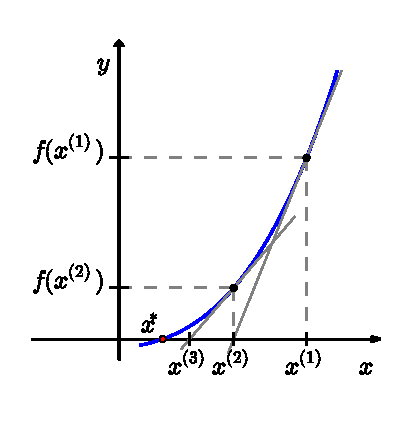
\includegraphics{./cap_equacao1d/pics/metodo_de_Newton/metodo_de_Newton.eps}
  \caption{Interpretação do método de Newton.}
  \label{fig:metodo_de_Newton}
\end{figure}

Ou seja, dada aproximação $x^{(n)}$, a próxima aproximação $x^{(n+1)}$ é o ponto de interseção entre o eixo das abscissas e a reta tangente ao gráfico da função no ponto $x = x^{(n)}$. Observe a Figura~\ref{fig:metodo_de_Newton}.

\subsection{Análise de convergência}\index{método de Newton-Raphson!convergência}\label{Analise_conv_Newton}

Seja $y = f(x)$ uma função com derivadas primeira e segunda contínuas tal que $f(x^*)=0$ e $f'(x^*)\neq 0$. Seja também a função $g(x)$ definida como:
\begin{equation}
  g(x)=x-\frac{f(x)}{f'(x)}.
\end{equation}
Expandindo em série de Taylor em torno de $x = x^*$, obtemos:
\begin{equation}
  g(x)=g(x^*)+g'(x^*)(x-x^*) + \frac{g''(x^*)}{2}(x-x^*)^2 + O\left((x-x^*)^3\right).
\end{equation}
Observamos que:
\begin{eqnarray}
g(x^*) &=& x^*\\
g'(x^*) &=& 1 - \frac{f'(x^*)f'(x^*)-f(x^*)f''(x^*)}{\left(f'(x^*)\right)^2} = 0
\end{eqnarray}
Portanto:
\begin{equation}
g(x) = x^* + \frac{g''(x^*)}{2}(x-x^*)^2 + O\left((x-x^*)^3\right)\\
\end{equation}
Com isso, temos:
\begin{equation}
x^{(n+1)} = g(x^{(n)}) =  x^*+ \frac{g''(x^*)}{2}(x^{(n)}-x^*)^2 + O\left((x^{(n)}-x^*)^3\right),
\end{equation}
ou seja, para $n$ suficientemente grande,
\begin{equation}
\left|x^{(n+1)}-x^*\right| \leq C\left|x^{(n)}-x^*\right|^2,
\end{equation}
com constante $C = \left|g''(x^*)/2\right|$. Isto mostra que o método de Newton tem \emph{taxa de convergência quadrática}. Mais precisamente, temos o seguinte teorema.

\begin{teo}[Método de Newton]
  Sejam $f\in C^2([a, b])$ com $x^*\in (a, b)$ tal que $f(x^*) = 0$ e:
  \begin{equation}
    m := \min_{x\in [a, b]}|f'(x)| > 0\quad\text{e}\quad M := \max_{x\in [a, b]} |f''(x)|.
  \end{equation}
Escolhendo $\rho > 0$ tal que:
\begin{equation}
  q := \frac{M}{2m}\rho < 1,
\end{equation}
definimos a \emph{bacia de atração} do método de Newton pelo conjunto:
\begin{equation}
  K_\rho(x^*) := \left\{x\in\mathbb{R};~|x-x^*| \leq \rho\right\}\subset [a, b].
\end{equation}
Então, para qualquer $x^{(1)}\in K_\rho(x^*)$ a iteração do método de Newton:
\begin{equation}
  x^{(n+1)} = x^{(n)} - \frac{f(x^{(n)})}{f'(x^{(n)})},
\end{equation}
fornece uma sequência $x^{(n)}$ que converge para $x^*$, isto é, $x^{(n)}\to x^*$ quando $n\to \infty$. Além disso, temos a seguinte estimativa de erro \emph{a priori}:
\begin{equation}
  |x^{(n)} - x^*| \leq \frac{2m}{M}q^{(2^{n-1})},\quad n\geq 2,
\end{equation}
e a seguinte estimativa de erro \emph{a posteriori}:
\begin{equation}
  |x^{(n)} - x^*| \leq \frac{M}{2m}|x^{(n)} - x^{(n-1)}|^2,\quad n\geq 2.
\end{equation}
\end{teo}
\begin{proof}
  Para $n\in\mathbb{N}$, $n\geq 2$, temos:
  \begin{equation}\label{eq:forma}
    x^{n+1}-x^* = x^{(n)} - \frac{f(x^{(n)})}{f'(x^{(n)})} - x^* = -\frac{1}{f'(x^{(n)})}\left[f(x^{(n)})+(x^*-x^{(n)})f'(x^{(n)})\right].
  \end{equation}
Agora, para estimar o lado direito desta equação, usamos o polinômio de Taylor de grau $1$ da função $f(x)$ em torno de $x = x^{(n)}$, isto é:
\begin{equation}
  f(x^*) = f(x^{(n)}) + (x^* - x^{(n)})f'(x^{(n)}) + \int_{x^{(n)}}^{x^*} f''(t)(x^* - t)\,dt.
\end{equation}
Pela mudança de variável $t = x^{(n)} + s(x^* - x^{(n)})$, observamos que o resto deste polinômio de Taylor na forma integral é igual a:
\begin{equation}
  R(x^*,x^{(n)}) := (x^* - x^{(n)})^2\int_0^1 f''\left(x^{(n)} + s(x^* - x^{(n)})\right)(1-s)\,ds.
\end{equation}
Assim, da cota da segunda derivada de $f(x)$, temos:
\begin{equation}\label{eq:est-resto}
  |R(x^*,x^{(n)})| \leq M|x^*-x^{(n)}|^2\int_0^1 (1-s)\,ds = \frac{M}{2}|x^* - x^{(n)}|^2.
\end{equation}\label{eq:quadratica}
Se $x^{(n)}\in K_\rho(x^*)$, então de \eqref{eq:forma} e \eqref{eq:est-resto} temos:
\begin{equation}
  |x^{(n+1)} - x^*| \leq \frac{M}{2m}|x^{(n)} - x^*|^2 \leq \frac{M}{2m}\rho^2 < \rho.
\end{equation}
Isto mostra que se $x^{(n)}\in K_\rho(x^*)$, então $x^{(n+1)}\in K_\rho(x^*)$, isto é, $x^{(n)}\in K_\rho(x^*)$ para todo $n\in\mathbb{R}$.

Agora, obtemos a estimativa \emph{a priori} de \eqref{eq:quadratica}, pois:
\begin{equation}
  |x^{(n)} - x^*| \leq \frac{2m}{M}\left(\frac{M}{2m}|x^{(n-1)}-x^*|\right)^2 \leq \cdots \leq \frac{2m}{M}\left(\frac{M}{2m} |x^{(1)}-x^*|\right)^{2^{n-1}}.
\end{equation}
Logo:
\begin{equation}
  |x^{(n)} - x^*| \leq \frac{2m}{M}q^{2^{n-1}},
\end{equation}
donde também vemos que $x^{(n)}\to x^*$ quando $n\to\infty$, pois $q < 1$.

Por fim, para provarmos a estimativa \emph{a posteriori} tomamos a seguinte expansão em polinômio de Taylor:
\begin{equation}
  f(x^{(n)}) = f(x^{(n-1)}) + (x^{(n)} - x^{(n-1)})f'(x^{(n-1)}) + R(x^{(n)},x^{(n-1)}).
\end{equation}
Aqui, temos:
\begin{equation}
  f(x^{(n-1)}) + (x^{(n)} - x^{(n-1)})f'(x^{(n-1)}) = 0
\end{equation}
e, então, conforme acima:
\begin{equation}
  |f(x^{(n)})| = |R(x^{(n)},x^{(n-1)})| \leq \frac{M}{2}|x^{(n)} - x^{(n-1)}|^2.
\end{equation}
Com isso e do teorema do valor médio, concluímos:
\begin{equation}
  |x^{(n)} - x^*| \leq \frac{1}{m}|f(x^{(n)}) - f(x^*)| \leq \frac{M}{2m}|x^{(n)} - x^{(n-1)}|^2.
\end{equation}
\end{proof}

\begin{ex}
  Estime o raio $\rho$ da bacia de atração $K_\rho(x^*)$ para a função $f(x) = \cos(x) - x$ restrita ao intervalo $[0, \pi/2]$.
\end{ex}
\begin{sol}
  O raio da bacia de atração é tal que:
  \begin{equation}
    \rho < \frac{2m}{M}
  \end{equation}
onde $m := \min |f'(x)|$ e $M := \max |f''(x)|$ com o mínimo e o máximo tomados em um intervalo $[a, b]$ que contenha o zero da função $f(x)$. Aqui, por exemplo, podemos tomar $[a, b] = [0, \pi/2]$. Como, neste caso, $f'(x) = -\sin(x) - 1$, temos que $m = 1$. Também, como $f''(x) = -\cos x$, temos $M = 1$. Assim, concluímos que $\rho < 2$ (lembrando que $K_\rho(x^*)\subset [0, \pi/2]$). Ou seja, neste caso as iterações de Newton convergem para o zero de $f(x)$ para qualquer escolha da aproximação inicial $x^{(1)}\in [0, \pi/2]$.
\end{sol}

\subsection*{Exercícios}

\begin{exer}\label{1d:cosx2}
Encontre a raiz positiva da função $f(x)=\cos(x)-x^2$ pelo método de Newton inicializando-o com $x^{(0)}=1$. Realize a iteração até obter estabilidade no $quinto$ dígito significativo.
\end{exer}
\begin{resp}
  raiz:0,82413, processo iterativo: $x^{(n+1)}= x^{(n)}+ \frac{\cos(x)-x^2}{\sin(x)+2x}$

%%%%%%%%%%%%%%%%%%%%
% scilab
%%%%%%%%%%%%%%%%%%%
\ifisscilab
\begin{verbatim}
-->x=1
-->x=x+(cos(x)-x^2)/(sin(x)+2*x)
-->x=x+(cos(x)-x^2)/(sin(x)+2*x)
-->x=x+(cos(x)-x^2)/(sin(x)+2*x)
-->x=x+(cos(x)-x^2)/(sin(x)+2*x)
\end{verbatim}
\fi
%%%%%%%%%%%%%%%%%%%%
%%%%%%%%%%%%%%%%%%%%
% octave
%%%%%%%%%%%%%%%%%%%
\ifisoctave
\begin{verbatim}
>> x=1
>> x=x+(cos(x)-x^2)/(sin(x)+2*x)
>> x=x+(cos(x)-x^2)/(sin(x)+2*x)
>> x=x+(cos(x)-x^2)/(sin(x)+2*x)
>> x=x+(cos(x)-x^2)/(sin(x)+2*x)
\end{verbatim}
\fi
%%%%%%%%%%%%%%%%%%%%
\end{resp}

\begin{exer} Considere o problema de calcular as soluções positivas da equação:
  \begin{equation}
    \tg(x)=2x^2.
  \end{equation}
\begin{itemize}
\item[a)] Use o método gráfico para isolar as duas primeiras raízes positivas em pequenos intervalos. Use a teoria para argumentar quanto à existência e unicidade das raízes dentro intervalos escolhidos.
% \item[b)] Calcule o número de iterações necessárias para que o método da bisseção aproxime cada uma das raízes com erro absoluto inferior a $10^{-8}$. Calcule as raízes por este método usando este número de passos.
\item[b)]  Calcule cada uma das raízes pelo método de Newton com oito dígitos significativos e discuta a convergência.% comparando com o item b).
\end{itemize}
%{\bf Obs:} Alguns alunos encontraram como solução $x_1\approx 1,5707963$ e $x_2 \approx 4,7123890$. O que eles fizeram de errado?
\end{exer}
%%%%%%%%%%%%%%%%%%%%
% scilab
%%%%%%%%%%%%%%%%%%%%
\ifisscilab
\begin{resp}
  \begin{itemize}
\item[a)]Primeiramente, deve-se observar que a função $\tg(x)$ não está definida quando $x$ é um múltiplo ímpar de $\frac{\pi}{2}$, pelo que devemos cuidado nas singularidades. Traçamos o gráfico da função $f(x)=\tg(x)-2x^2$ no \verb+Scilab+ usando os seguintes comandos:
\begin{verbatim}
-->deff('y=f(x)','y=tan(x)-2*x^2')
-->plot([0:.01:1.3],f)
\end{verbatim}
Observamos facilmente uma raiz no intervalo $(0,5, 0,6)$ e outra no intervalo $(1,2, 1,3)$. Como a função $f(x)$ é contínua fora dos pontos de singularidade da tangente, é fácil verificar que existe pelo menos uma solução nos intervalos dados pelo teorema de Bolzano~\ref{teo:teorema_de_Bolzano}:
\begin{eqnarray}
f(0,5) &\approx& 0,046302 >0\\
f(0,6) &\approx& -0,035863 <0\\
f(1,2) &\approx& -0,30784e-1 <0\\
f(1,3) &\approx&  0,22210e-1>0\\
\end{eqnarray}
Para provar a unicidade da solução em cada intervalo, precisamos mostra que a função é monótona, ou seja, a derivada não muda de sinal em cada intervalo:
\begin{eqnarray}
f'(x)=\sec^2(x)-4x=\frac{1}{\cos^2(x)}-4x\leq \frac{1}{\cos^2(0,6)}-4*0,5<0, ~~x\in[ 0,5, 0,6]\\
f'(x)=\sec^2(x)-4x=\frac{1}{\cos^2(x)}-4x\geq \frac{1}{\cos^2(1,2)}-4*1,3>0, ~~x\in[ 1,2, 1,3]\\
\end{eqnarray}

% \item[b)]
% Já isolamos as raízes em intervalos de comprimento $10^{-1}$ e a precisão requerida exige que as isolemos em intervalos de comprimento $2\times 10^{-8}$. Como cada passo da bisseção, confina a raiz em um intervalo com comprimento igual à metade do comprimento do intervalo anterior, temos a seguinte condição para o número de passos $N_p$:
% \begin{equation} \frac{10^{-1}}{2^N_p}\leq 2\times 10^{-8} \end{equation}
% isso é equivalente a
% \begin{equation} N_p\geq \log_2 \frac{10^{-1}}{2\times 10^{-8}}=\log_2 \frac{10^{7}}{2}=7\log_2 10 -1=\frac{7}{\log_10 2}-1\approx 22.22 \end{equation}
% Como $N_p$ é inteiro, o menor $N_p$ que satisfaz a condição é $23$.

% As raízes obtidas são $0.55970415$ e $1.2703426$.

\item[b)] Para recalcular as raízes pelo método de Newton, basta executar a iteração:
\begin{equation} x^{(n+1)}=x^{(n)}-\frac{f(x^{(n)})}{f'(x^{(n)}}. \end{equation}
\end{itemize}
Em relação à observação, o erro se deveu à falta de cuidado em compreender o problema antes de tentar resolvê-lo, em especial, à falta de observar que a função é descontínua em  múltiplos ímpares de $\frac{\pi}{2}$. Nestes pontos, a função $f(x)$ troca de sinal, mas não passa por zero.
\end{resp}
\fi
%%%%%%%%%%%%%%%%%%%%


\begin{exer}\label{new1} Considere a equação
  \begin{equation} e^{-x^2}=x \end{equation}
trace o gráfico com auxílio do computador e verifique que ela possui uma raiz positiva. Encontre uma aproximação para esta raiz pelo gráfico e use este valor para inicializar o método de Newton e obtenha uma aproximação para a raiz com 8 dígitos significativos. \ifisscilab (Use o comando \verb+format('v',16)+ para alterar a visualização no \verb+Scilab+.)\fi
\end{exer}
\begin{resp}
  0,65291864
  \end{resp}

\begin{exer}\label{new2} Isole e encontre as cinco primeiras raízes positivas da equação com 6 dígitos corretos através de traçado de gráfico e do método de Newton.
\begin{equation} \cos(10x)=e^{-x}. \end{equation} Dica: a primeira raiz positiva está no intervalo $(0, 0,02)$. Fique atento.
\end{exer}
\begin{resp}
   $0,0198679$; $0,533890$; $0,735412$; $1,13237$ e $1,38851$.
  \end{resp}


\begin{exer}\label{new3} Encontre as raízes do polinômio $f(x)=x^4-4x^2+4$ através do método de Newton. O que você observa em relação ao erro obtido? Compare com a situação do Problema~\ref{prob_raiz_dupla}.
\end{exer}

\begin{exer}\label{new4} Encontre as raízes reais do polinômio $f(x)=\frac{x^5}{100}+x^4+3x+1$ isolando-as pelo método do gráfico e depois usando o método de Newton. Expresse a solução com 7 dígitos significativos.
\end{exer}
\begin{resp}
 $-99.99970$, $-0.3376513$; $-1.314006$.
 \end{resp}

\begin{exer}Considere o método de Newton aplicado para encontrar a raiz de $f(x)=x^3-2x+2$. O que acontece quando $x^{(0)}=0$? Escolha um valor adequado para inicializar o método e obter a única raiz real desta equação.
\end{exer}

\begin{exer} Justifique a construção do processo iterativo do método de Newton através do conceito de estabilidade de ponto fixo e convergência do método da iteração. Dica: Considere os problemas \ref{int_new1} e \ref{int_new2}.
\end{exer}

\begin{exer} Entenda a interpretação geométrica ao método de Newton. Encontre uma valor para iniciar o método de Newton aplicado ao problema $f(x)=xe^{-x}=0$ tal que o esquema iterativo divirja.
\end{exer}
\begin{resp}

$x_0>1$.

\end{resp}

\begin{exer}(Computação) Aplique o método de Newton à função $f(x)=\frac{1}{x}-A$ e construa um esquema computacional para calcular a inversa de $A$ com base em operações de multiplicação e soma/subtração.
 \end{exer}
\begin{resp}
  \begin{eqnarray}
 x^{(0)} &=& \text{C.I.}\\
 x^{(n+1)}&=&x^{(n)}\left(2-Ax^{(n)}\right) \\
 \end{eqnarray}
\end{resp}


\begin{exer}(Computação) Aplique o método de Newton à função $f(x)=x^n-A$ e construa um esquema computacional para calcular  $\sqrt[n]{A}$ para $A>0$ com base em operações de multiplicação e soma/subtração.
\end{exer}
\begin{resp}
 \begin{eqnarray}
 x_{0} &=& \text{C.I.}\\
 x^{(n+1)}&=&x^{(n)}\left(1-\frac{1}{n}\right) + \frac{A}{n x^{(n)}}
 \end{eqnarray}

\end{resp}


\begin{exer}(Computação) Aplique o método de Newton à função $f(x)=\frac{1}{x^2}-A$ e construa um esquema computacional para calcular  $\frac{1}{\sqrt{A}}$ para $A>0$ com base em operações de multiplicação e soma/subtração.
\end{exer}
\begin{resp}
 \begin{eqnarray}
 x_{0} &=& \text{C.I.}\\
 x^{(n+1)}&=&x^{(n)} + \frac{x^{(n)}-Ax^{(n)}}{2}=\frac{(3-A)x^{(n)}}{2}\\
 \end{eqnarray}

\end{resp}




\begin{exer} Considere a função dada por
\begin{eqnarray}
\psi(x)&=&\ln\left(15-\ln(x)\right)
\end{eqnarray}
definida para $x\in \left(0,e^{15}\right)$
\begin{itemize}
\item [a)] Use o teorema do ponto fixo para provar que se $x^{(0)}$ pertence ao intervalo $[1,3]$, então a sequência dada iterativamente por \begin{equation} x^{(n+1)}=\psi(x^{(n)}),n\geq 0 \end{equation} converge para o único ponto fixo, $x^*$, de $\psi$. Construa a iteração $x^{(n+1)}=\psi(x^{(n)})$ e obtenha numericamente o valor do ponto fixo $x^*$. Expresse a resposta com 5 algarismos significativos corretos.
\item [b)] Construa a iteração do método de Newton para encontrar $x^*$, explicitando a relação de recorrência e iniciando com $x_0=2$. Use o computador para obter a raiz e expresse a resposta com oito dígitos significativos corretos.
\end{itemize}
\end{exer}

\section{Método das secantes}\index{método das secantes}

O \emph{método das secantes} é uma variação do método de Newton, evitando a necessidade de conhecer-se a derivada analítica de $f(x)$. Dada uma função $f(x)$, a ideia é aproximar sua derivada pela razão fundamental:
\begin{equation}
  f'(x)\approx \frac{f(x)-f(x_0)}{x-x_0},\quad x\approx x_0.
\end{equation}

Mais precisamente, o método de Newton é uma iteração de ponto fixo da forma:
\begin{equation}
  x^{(n+1)} = x^{(n)} - \alpha(x^{(n)})f(x^{(n)}),\quad n\geq 1,
\end{equation}
onde $x^{(1)}$ é uma aproximação inicial dada e $\alpha(x^{(n)}) = 1/f'(x^{(n)})$. Usando a aproximação da derivada acima, com $x = x^{(n)}$ e $x_0 = x^{(n-1)}$, temos:
\begin{equation}
  \alpha(x^{(n)}) = \frac{1}{f'(x^{(n)})} \approx  \frac{x^{(n)} - x^{(n-1)}}{f(x^{(n)}) - f(x^{(n-1)})}.
\end{equation}
Isto nos motiva a introduzir a \emph{iteração do método das secantes} dada por:
\begin{equation}
  x^{(n+1)} = x^{(n)} - f(x^{(n)})\frac{x^{(n)} - x^{(n-1)}}{f(x^{(n)}) - f(x^{(n-1)})},\quad n\geq 2.
\end{equation}
Observe que para inicializarmos a iteração acima precisamos de duas aproximações iniciais, a saber, $x^{(1)}$ e $x^{(2)}$. Maneiras apropriadas de escolher estas aproximações podem ser inferidas da interpretação geométrica do método.

\begin{ex} Encontre as raízes de $f(x)=\cos(x)-x$.
\end{ex}
\begin{sol}
Da inspeção do gráfico das funções $y=\cos(x)$ e $y=x$, sabemos que esta equação possui uma raiz em torno de $x=0,8$. Iniciamos o método com $x_0=0,7$ e $x_1=0,8$.
\begin{center}
\begin{tabular}{|c|c|c|c|}\hline
$x^{(n-1)}$ & $x^{(n)}$ & $m$ & $x^{(n+1)}$\\\hline
 & & $\frac{f(0,8)-f(0,7)}{0,8-0,7} =$ & $0,8- \frac{f(0,8)}{-1,6813548}=$\\
$0,7$ & $0,8$ & $-1,6813548$ & $0,7385654$\\\hline
$0,8$ & $0,7385654$ & $-1,6955107$ & $0,7390784$ \\\hline
 $0,7385654$ & $0,7390784$ &  $-1,6734174$ & $0,7390851$ \\\hline
$0,7390784$ & $0,7390851$ & $-1,6736095$ & $0,7390851$ \\\hline
\end{tabular}
\end{center}
\end{sol}

\subsection{Interpretação geométrica}

Enquanto, o método de Newton está relacionado às retas tangentes ao gráfico da função objetivo $f(x)$, o método das secantes, como o próprio nome indica, está relacionado às retas secantes.

\begin{figure}[h]
  \centering
  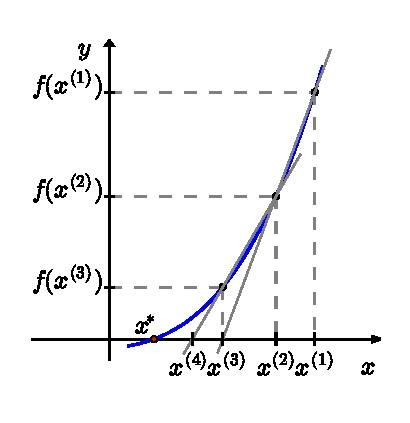
\includegraphics{./cap_equacao1d/pics/metodo_das_secantes/metodo_das_secantes.eps}
  \caption{Método das secantes.}
  \label{fig:metodo_das_secantes}
\end{figure}

Sejam $f(x)$ e as aproximações $x^{(1)}$ e $x^{(2)}$ do zero $x^*$ desta função (veja Figura~\ref{fig:metodo_das_secantes}). A iteração do método das secantes fornece:
\begin{equation}
  x^{(3)} = x^{(2)} - f(x^{(2)})\frac{x^{(2)} - x^{(1)}}{f(x^{(2)}) - f(x^{(1)})}.
\end{equation}
De fato, $x^{(3)}$ é o ponto de interseção da reta secante ao gráfico de $f(x)$ pelos pontos $x^{(1)}$ e $x^{(2)}$ com o eixo das abscissas. Com efeito, a equação desta reta secante é:
\begin{equation}
  y = \frac{f(x^{(2)}) - f(x^{(1)})}{x^{(2)} - x^{(1)}}(x - x^{(2)}) + f(x^{(2)}).
\end{equation}
Esta reta intercepta o eixo das abscissas no ponto $x$ tal que $y=0$, isto é:
\begin{equation}
  \frac{f(x^{(2)}) - f(x^{(1)})}{x^{(2)} - x^{(1)}}(x - x^{(2)}) + f(x^{(2)}) = 0
  \Rightarrow x = x^{(2)} - f(x^{(2)})\frac{x^{(2)} - x^{(1)}}{f(x^{(2)}) - f(x^{(1)})}.
\end{equation}


\subsection{Análise de convergência}\index{método das secantes!convergência}

Uma análise assintótica semelhante àquela feita para o método de Newton na subseção~\ref{Analise_conv_Newton} nos indica que, para uma função $f(x)$ duas vezes diferenciável, as iterações do método da secante satisfazem:
\begin{equation}
  |x^{(n+1)} - x^*| \approx C |x^{(n)} - x^*||x^{(n-1)} - x^*|,
\end{equation}
para aproximações iniciais suficientemente próximas de $x^*$, onde $f(x^*) = 0$. Além disso, veremos que:
\begin{equation}
  |x^{(n+1)} - x^*| \leq C |x^{(n)} - x^*|^{p},~~ p=\frac{\sqrt{5}+1}{2}\approx 1,618
\end{equation}
sob certas condições. Ou seja, o método das secantes tem \emph{taxa de convergência superlinear}.

\begin{teo}[Método das secantes]\label{teo:metodo_das_secantes}
  Seja $f\in C^2([a, b])$ uma função com $x^*\in (a, b)$ tal que $f(x^*) = 0$. Sejam, também:
  \begin{equation}
    m := \min_{x\in [a, b]} |f'(x)| > 0\quad\text{e}\quad M := \max_{x\in [a,b]} |f''(x)| < \infty.
  \end{equation}
Além disso, seja $\rho > 0$ tal que:
\begin{equation}
  q := \frac{M}{2m}\rho < 1,\quad K_\rho(x^*) := \{x\in\mathbb{R};~|x-x^*|\leq \rho\}\subset [a, b].
\end{equation}
Então, para aproximações iniciais $x^{(1)}, x^{(2)}\in K_\rho(x^*)$, com $x^{(1)}\neq x^{(2)}$, temos que as iterações do método das secantes $x^{(n)}\in K_\rho(x^*)$, $n\geq 1$, e $x^{(n)}\to x^*$, quando $n\to\infty$. Além disso, vale a seguinte estimativa de convergência \emph{a priori}:
\begin{equation}
  |x^{(n)} - x^*| \leq \frac{2m}{M}q^{\gamma_{n-1}},\quad n\geq 1,
\end{equation}
onde $\{\gamma_n\}_{n\in\mathbb{N}}$ é a sequência de Fibonacci\footnote{Leonardo Fibonacci, c. 1170 - c. 1250, matemático italiano.}\footnote{A sequência de Fibonacci $\{\gamma_n\}_{n\in\mathbb{N}}$ é definida por $\gamma_0 = \gamma_1 = 1$ e $\gamma_{n+1} = \gamma_{n} - \gamma_{n-1}$, $n\geq 1$.}, bem como vale a estimativa \emph{a posteriori}:
\begin{equation}
  |x^{(n)} - x^*| \leq \frac{M}{2m}|x^{(n)}-x^{(n-1)}||x^{(n-1)}-x^{(n-2)}|,\quad n\geq 3.
\end{equation}
\end{teo}
\begin{proof}
  Sejam $n\in\mathbb{N}$ com $n\geq 2$ e $x^{(n)}, x^{(n-1)}\in K_\rho(x^*)$, tal que $x^{(n)}\neq x^{(n-1)}$, $x^{(n)}\neq x^*$ e $x^{(n-1)}\neq x^*$. Seja, também:
  \begin{equation}
    g(x^{(n)},x^{(n-1)}) := x^{(n)} - f(x^{(n)})\frac{x^{(n)} - x^{(n-1)}}{f(x^{(n)}) - f(x^{(n-1)})}.
  \end{equation}
Com isso, temos:
  \begin{eqnarray}
    &&g(x^{(n)},x^{(n-1)}) - x^* = x^{(n)} - f(x^{(n)})\frac{x^{(n)} - x^{(n-1)}}{f(x^{(n)}) - f(x^{(n-1)})} - x^*\\
    &=& \frac{x^{(n)} - x^{(n-1)}}{f(x^{(n)}) - f(x^{(n-1)})}\left\{(x^{(n)} - x^*)\frac{f(x^{(n)}) - f(x^{(n-1)})}{x^{(n)} - x^{(n-1)}}\right.\\ &\ &\qquad\qquad\qquad\qquad\qquad -\left. f(x^{(n)}) + f(x^*)\right\}.\\
  \end{eqnarray}
Então, da cota assumida para primeira derivada de $f(x)$ e do teorema do valor médio, temos:
\begin{equation}\label{eq:secantes-est0}
  |g(x^{(n)},x^{(n-1)}) - x^*| \leq \frac{|x^{(n)} - x^*|}{m}\left|\frac{f(x^{(n)}) - f(x^{(n-1)})}{x^{(n)} - x^{(n-1)}} - \frac{f(x^{(n)}) - f(x^*)}{x^{(n)} - x^*}\right|.
\end{equation}
Agora, iremos estimar este último termo a direita. Para tanto, começamos observando que da expansão em polinômio de Taylor de ordem $0$ da função $f(x)$ com resto na forma integral, temos:
\begin{eqnarray}
  \frac{f(x^{(n)}) - f(x^{(n-1)})}{x^{(n)} - x^{(n-1)}} &= -\int_0^1 \frac{d}{dr}f(x^{(n)} + r(x^{(n-1)} - x^{(n)}))\frac{dr}{x^{(n)} - x^{(n-1)}}\\
  &= \int_0^1 f'(x^{(n)} + r(x^{(n-1)} - x^{(n)}))\,dr
\end{eqnarray}
De forma análoga, temos:
\begin{equation}
  \frac{f(x^{(n)}) - f(x^*)}{x^{(n)} - x^*} = \int_0^1 f'(x^{(n)} + r(x^* - x^{(n)}))\,dr
\end{equation}
Logo, temos:
\begin{equation}\label{eq:secantes-0}
  \begin{split}
  &\frac{f(x^{(n)}) - f(x^{(n-1)})}{x^{(n)} - x^{(n-1)}} - \frac{f(x^{(n)}) - f(x^*)}{x^{(n)} - x^*} = \\
  &\int_0^1 \left[f'(x^{(n)} + r(x^{(n-1)} - x^{(n)})) - f'(x^{(n)} + r(x^* - x^{(n)}))\right]\,dr.
  \end{split}
\end{equation}
Agora, novamente temos:
\begin{equation}
  \begin{split}
  &f'(x^{(n)} + r(x^{(n-1)} - x^{(n)})) - f'(x^{(n)} + r(x^* - x^{(n)}))\\
  &= \int_0^r \frac{d}{ds}f'(x^{(n)} + r(x^{(n-1)} - x^{(n)}) + s(x^* - x^{(n-1)}))\,ds\\
  &= \int_0^r f''(x^{(n)} + r(x^{(n-1)} - x^{(n)}) + s(x^* - x^{(n-1)}))\,ds(x^* - x^{(n-1)}).
  \end{split}
\end{equation}
Retornando à Equação~\eqref{eq:secantes-0} e usando a cota para a segunda derivada, obtemos:
\begin{equation}
  \left|\frac{f(x^{(n)}) - f(x^{(n-1)})}{x^{(n)} - x^{(n-1)}} - \frac{f(x^{(n)}) - f(x^*)}{x^{(n)} - x^*} \right| \leq \frac{M}{2}|x^{(n-1)} - x^*|.
\end{equation}
Utilizando a Equação~\eqref{eq:secantes-est0}, obtemos:
\begin{equation}
  |g(x^{(n)},x^{(n-1)})-x^*| \leq \frac{M}{2m}|x^{(n)}-x^*||x^{(n-1)}-x^*| \leq \frac{M}{2m}\rho^2 < \rho.
\end{equation}
Portanto, concluímos que as iterações do método da secantes $x^{(n)}$ permanecem no conjunto $K_\rho(x^*)$, se começarem nele. Além disso, temos demonstrado que:
\begin{equation}
  |x^{(n+1)} - x^*| \leq \frac{M}{2m}|x^{(n)} - x^*||x^{(n-1)} - x^*|.
\end{equation}
Com isso, temos:
\begin{equation}
  \rho_n := \frac{M}{2m}|x^{(n)} - x^*| \Rightarrow \rho_{n+1} \leq \rho_{n}\rho_{n-1},\quad n\geq 2.
\end{equation}
Como $\rho_1 \leq q$ e $\rho_2 \leq q$, temos $\rho_n \leq q^{\gamma_{n-1}}$, $n\geq 1$. Isto mostra a estimativa de convergência \emph{a priori}:
\begin{equation}
  |x^{n} - x^*| \leq \frac{2m}{M}q^{\gamma_{n-1}}.
\end{equation}
Além disso, como $\gamma_{n}\to \infty$ quando $n\to\infty$ e $q < 1$, temos que as iterações do método das secantes $x^{(n)}\to x^*$ quando $n\to \infty$.

Por fim, mostramos a estimativa de convergência \emph{a posteriori}. Para tanto, da cota assumida para a primeira derivada e do teorema do valor médio, temos, para $n\geq 3$:
\begin{eqnarray}
  |x^{(n)} - x^*| &\leq& \frac{1}{m}|f(x^{(n)} - f(x^*)|\\
  &=& \frac{1}{m}\left|f(x^{(n-1)}) + (x^{(n)} - x^{(n-1)})\frac{f(x^{(n)}) - f(x^{(n-1)})}{x^{(n)} - x^{(n-1)}}\right|\\
  &=& \frac{1}{m}\left|x^{(n)} - x^{(n-1)}\right|\left|\frac{f(x^{(n)}) - f(x^{(n-1)})}{x^{(n)} - x^{(n-1)}} + \frac{f(x^{(n-1)})}{x^{(n)} - x^{(n-1)}}\right|.
\end{eqnarray}
Agora, a iteração do método das secantes fornece:
\begin{equation}
  x^{(n)} = x^{(n-1)} - f(x^{(n-1)})\frac{x^{(n-1)} - x^{(n-2)}}{f(x^{(n-1)}) - f(x^{(n-2)})}
\end{equation}
e temos:
\begin{equation}
  \frac{f(x^{(n-1)})}{x^{(n)} - x^{(n-1)}} = -\frac{f(x^{(n-1)}) - f(x^{(n-2)})}{x^{(n-1)} - x^{(n-2)}}.
\end{equation}
Portanto:
\begin{equation}
  |x^{(n)} - x^*| \leq \frac{1}{m}|x^{(n)} - x^{(n-1)}|\left|\frac{f(x^{(n-1)}) - f(x^{(n)})}{x^{(n-1)} - x^{(n)}} - \frac{f(x^{(n-1)}) - f(x^{(n-2)})}{x^{(n-1)} - x^{(n-2)}}\right|.
\end{equation}
Observamos que o último termo pode ser estimado como feito acima para o termo análogo na Inequação~\eqref{eq:secantes-est0}. Com isso, obtemos a estimativa desejada:
\begin{equation}
  |x^{(n)} - x^*| \leq \frac{M}{2m}|x^{(n)} - x^{(n-1)}||x^{(n)} - x^{(n-2)}|.
\end{equation}
\end{proof}

\begin{prop}[Sequência de Fibonacci]\label{prop:sequencia_de_Fibonacci}\index{sequência de!Fibonacci}
  A sequência de Fibonacci $\{\gamma_n\}_{n\in\mathbb{N}}$ é assintótica a $\gamma_n \sim \lambda_1^{n+1}/\sqrt{5}$ e:
\begin{equation}
  \lim_{n\to\infty} \frac{\gamma_{n+1}}{\gamma_{n}} = \lambda_1,
\end{equation}
onde $\lambda_1 = (1+\sqrt{5})/2\approx 1,618$ é a porção áurea\index{porção áurea}.
\end{prop}
\begin{proof}
  A sequência de Fibonacci $\{\gamma_n\}_{n\in\mathbb{N}}$ é definida por $\gamma_0 = \gamma_1 = 1$ e $\gamma_{n+1} = \gamma_n + \gamma_{n-1}$, $n\geq 1$. Logo, satisfaz a seguinte equação de diferenças:
  \begin{equation}
    \gamma_{n+2} - \gamma_{n+1} - \gamma_{n} = 0,\quad n\in\mathbb{N}.
  \end{equation}
Tomando $\gamma_n = \lambda^n$, $\lambda\neq 0$ temos:
\begin{equation}
  \lambda^n\left(\lambda^2 - \lambda - 1\right) = 0 \Rightarrow   \lambda^2 - \lambda - 1 = 0 \Rightarrow \lambda_{1,2} = \frac{1 \pm \sqrt{5}}{2}.
\end{equation}
Portanto, $\gamma_n = c_1\lambda_1^n + c_2\lambda_2^n$. Como $\gamma_0 = \gamma_1 = 1$, as constantes satisfazem:
\begin{equation}
  \begin{array}{l}
    c_1 + c_2 = 1\\
    c_1\lambda_1 + c_2\lambda_2 = 1
  \end{array}
    \Rightarrow
    c_1 = \frac{1+\sqrt{5}}{2\sqrt{5}},\quad c_2 = -\frac{1-\sqrt{5}}{2\sqrt{5}}.
\end{equation}
Ou seja, obtemos a seguinte forma explícita para os números de Fibonacci:
\begin{equation}
  \gamma_n = \frac{1}{\sqrt{5}}\left[\left(\frac{1+\sqrt{5}}{2}\right)^{n+1} - \left(\frac{1-\sqrt{5}}{2}\right)^{n+1}\right].
\end{equation}
Daí, segue imediatamente o enunciado.
\end{proof}

\begin{obs}
  Sob as hipóteses do Teorema~\ref{teo:metodo_das_secantes} e da Proposição~\ref{prop:sequencia_de_Fibonacci}, temos:
  \begin{eqnarray}
    \lim_{n\to\infty} \frac{|x^{(n+1)}-x^*|}{|x^{(n)} - x^*|^{\lambda_1}} &\leq& \lim_{n\to\infty} \frac{M}{2m}|x^{(n)}-x^*|^{1-\lambda_1}|x^{(n-1)}-x^*| \\
    &\leq& \lim_{n\to\infty} \left(\frac{2m}{M}\right)^{1-\lambda_1}q^{(2-\lambda_1)\lambda_1^{n}/\sqrt{5}} = 0.
  \end{eqnarray}
Isto mostra que o método das secantes (nestas hipóteses) tem taxa de convergência superlinear ($\lambda_1 \approx 1,6$).
\end{obs}


\section{Critérios de parada}

Quando usamos métodos iterativos precisamos determinar um critério de parada. A Tabela~\ref{tab:quadro_comparativo} indica critérios de parada usuais para os métodos que estudamos neste capítulo.

\begin{table}[h!]
  \centering
  \caption{Quadro comparativo.}
  \label{tab:quadro_comparativo}
  {\small
  \begin{tabular}[h!]{cccc} \hline
    Método & Convergência & Erro & Critério de parada \\ \hline
    \multirow{2}{*}{Bisseção} & Linear & \multirow{2}{*}{$\displaystyle \epsilon_{n+1}=\frac{1}{2}\epsilon$} & \multirow{2}{*}{$\displaystyle \frac{b_n - a_n}{2} < \text{erro}$} \\
    & ($p=1$) & & \\
    & & & \\
    Iteração & Linear & \multirow{2}{*}{$\displaystyle \epsilon_{n+1}\approx |\phi'(x^*)| \varepsilon_{n}$} & \multirow{2}{*}{$\displaystyle \begin{array}{cc} \frac{|\Delta_n|}{1-\frac{\Delta_n}{\Delta_{n-1}}}< \text{erro} \\ \Delta_{n} < \Delta_{n-1}\end{array}$} \\
    linear                 & ($p=1$) & & \\
    & & & \\
    \multirow{2}{*}{Newton} & Quadrática & \multirow{2}{*}{$\displaystyle \epsilon_{n+1}\approx \frac{1}{2}\left|\frac{f''(x^*)}{f'(x^*)}\right|\varepsilon_{n}^2$} & \multirow{2}{*}{$|\Delta_n|< \text{erro}$} \\
    & ($p=2$) & & \\
    & & & \\
    \multirow{3}{*}{Secante} & \multirow{3}{*}{$\displaystyle \begin{array}{rl} p &= {\displaystyle \frac{\sqrt{5}+1}{2}}\\
  &\approx 1,618\end{array}$} & \multirow{3}{*}{$\displaystyle \begin{array}{rl} \varepsilon_{n+1} &\approx \displaystyle \left|\frac{f''(x^*)}{f'(x^*)}\right| \varepsilon_{n}\varepsilon_{n-1} \\
    &\approx M \varepsilon_{n}^\phi\end{array}$} & \multirow{3}{*}{$|\Delta_n|< \text{erro}$}\\
    & & & \\
    & & & \\
    & & & \\ \hline
  \end{tabular}
}
\end{table}


\begin{obs}
O erro na tabela sempre se refere ao erro absoluto esperado. Nos três últimos métodos, é comum que se exija como critério de parada que a condição seja satisfeita por alguns poucos passos consecutivos. Outros critérios podem ser usados. No métodos das secantes, deve-se ter o cuidado de evitar divisões por zero quando $x_{n+1}-x_n$ muito pequeno em relação à resolução do sistema de numeração.
\end{obs}

\subsection*{Exercícios}

\begin{exer} Refaça as questões \ref{new1}, \ref{new2}, \ref{new3}  e \ref{new4}, usando o método das secantes.
\end{exer}

\begin{exer} Dê uma interpretação geométrica ao método das secantes. Qual a vantagem do método das secantes sobre o método de Newton?
\end{exer}

\begin{exer} Aplique o método das secantes para resolver a equação
  \begin{equation}
    e^{-x^2}=2x
  \end{equation}
\end{exer}

\begin{exer} Refaça o Problema~\ref{prob_diodo} usando o método de Newton e das secantes.
\end{exer}

\begin{exer}
  Seja uma função $f(x)$ dada duas vezes continuamente diferenciável. Faça uma análise assintótica para mostrar que as iterações do método das secantes satisfazem:
  \begin{equation}
    |x^{(n+1)} - x^*| \approx C |x^{(n)} - x^*||x^{(n-1)} - x^*|,
  \end{equation}
para aproximações iniciais $x^{(1)}$ e $x^{(2)}$ suficientemente próximas de $x^*$, onde $f(x^*) = 0$.
\end{exer}
\begin{resp}
Seja $f(x)\in C^2$ um função tal que $f(x^*)=0$ e $f'(x^*)\neq 0$. Considere o processo iterativo do método das secantes:
\begin{equation} x^{(n+1)}=x^{(n)}- \frac{f(x^{(n)})}{f(x^{(n)})-f(x^{(n-1)})}(x^{(n)}-x^{(n-1)}) \end{equation}
Esta expressão pode ser escrita como:
\begin{eqnarray}
x^{(n+1)}&=&x^{(n)}- \frac{f(x^{(n)})(x^{(n)}-x^{(n-1)})}{f(x^{(n)})-f(x^{(n-1)})}\\~\\
 &=&\frac{x^{(n)}\left(f(x^{(n)})-f(x^{(n-1)})\right)-f(x^{(n)})(x^{(n)}-x^{(n-1)})}{f(x^{(n)})-f(x^{(n-1)})}\\
 &=&\frac{x^{(n)} f(x^{(n-1)})-x^{(n-1)}f(x^{(n)})}{f(x^{(n)})-f(x^{(n-1)})}
\end{eqnarray}

Subtraindo $x^*$ de ambos os lados temos:
\begin{eqnarray}
x^{(n+1)}-x^*
 &=&\frac{x^{(n)} f(x^{(n-1)})-x^{(n-1)}f(x^{(n)})}{f(x^{(n)})-f(x^{(n-1)})}-x^*\\
 &=&\frac{x^{(n)} f(x^{(n-1)})-x^{(n-1)}f(x^{(n)})-x^*\left(f(x^{(n)})-f(x^{(n-1)})\right)}{f(x^{(n)})-f(x^{(n-1)})}\\
 &=&\frac{(x^{(n)}-x^*) f(x^{(n-1)})-(x^{(n-1)}-x^*)f(x^{(n)})}{f(x^{(n)})-f(x^{(n-1)})}
\end{eqnarray}

Definimos $\epsilon_n=x_n-x^*$, equivalente a $x_n=x^*+\epsilon_n$
\begin{eqnarray}
\epsilon_{n+1}
 &=&\frac{\epsilon_n f(x^*+\epsilon_{n-1})-\epsilon_{n-1}f(x^*+\epsilon_n)}{f(x^*+\epsilon_n)-f(x^*+\epsilon_{n-1})}
\end{eqnarray}

Aproximamos a função $f(x)$ no numerador por
\begin{eqnarray}
f(x^*+\epsilon)&\approx& f(x^*)+\epsilon f'(x^*) + \epsilon^2 \frac{f''(x^*)}{2}\\
f(x^*+\epsilon)&\approx& \epsilon f'(x^*) + \epsilon^2 \frac{f''(x^*)}{2}
\end{eqnarray}

\begin{eqnarray}
\epsilon_{n+1} &\approx&\frac{\epsilon_n \left[\epsilon_{n-1} f'(x^*) + \epsilon_{n-1}^2 \frac{f''(x^*)}{2}\right]-\epsilon_{n-1}\left[\epsilon_{n} f'(x^*) + \epsilon_{n}^2 \frac{f''(x^*)}{2}\right]}{f(x^*+\epsilon_n)-f(x^*+\epsilon_{n-1})}\\
&=&\frac{\frac{f''(x^*)}{2}\left(\epsilon_{n}\epsilon_{n-1}^2-\epsilon_{n-1}\epsilon_{n}^2\right)}{f(x^*+\epsilon_n)-f(x^*+\epsilon_{n-1})}\\
&=&\frac{1}{2}f''(x^*)\frac{\epsilon_{n}\epsilon_{n-1}\left(\epsilon_{n-1}-\epsilon_{n}\right)}{f(x^*+\epsilon_n)-f(x^*+\epsilon_{n-1})}
\end{eqnarray}

Observamos, agora, que
\begin{equation}
  \begin{split}
  f(x^*+\epsilon_n)-f(x^*+\epsilon_{n-1}) &\approx \left[f(x^*)+f'(x^*)\epsilon_n\right]-\left[f(x^*)+f'(x^*)\epsilon_{n-1}\right] \\
  &=f'(x^*)(\epsilon_n-\epsilon_{n-1})
  \end{split}
\end{equation}

Portanto:
\begin{equation}
  \epsilon_{n+1}\approx \frac{1}{2}\frac{f''(x^*)}{f'(x^*)} \epsilon_n \epsilon_{n-1}
\end{equation}
ou, equivalentemente:
\begin{equation}
  x^{(n+1)}-x^*\approx \frac{1}{2}\frac{f''(x^*)}{f'(x^*)} \left(x^{(n)}-x^*\right) \left(x^{(n-1)}-x^*\right)
\end{equation}
\end{resp}

\section{Exercícios finais}

\begin{exer} Calcule uma equação da reta tangente a curva $y=e^{-(x-1)^2}$ que passa pelo ponto $(3, 1/2)$.
\end{exer}

\begin{exer} Resolva numericamente a inequação:
  \begin{equation}
    e^{-x^2}<2x
  \end{equation}
\end{exer}
\begin{resp}

    $x>a$ com $a\approx 0,4193648$.

\end{resp}


\begin{exer} A equação \begin{equation} \cos(\pi x)=e^{-2x} \end{equation} tem infinitas raízes.
Usando  métodos numéricos encontre as primeiras raízes dessa equação. Verifique a $j$-ésima raiz ($z_j$) pode ser aproximada por $j-1/2$ para $j$ grande. Use o método de Newton para encontrar uma aproximação melhor para $z_j$.
\end{exer}
\begin{resp}

 $z_1\approx 0.3252768 $, $z_2\approx 1.5153738$, $z_3\approx 2.497846  $, $z_4\approx 3.5002901$, $z_j\approx j-1/2-(-1)^j\frac{e^{-2j+1}}{\pi}, ~~~j>4$

\end{resp}


\begin{exer}(Eletricidade) A corrente elétrica, $I$, em Ampéres em uma lâmpada em função da tensão elétrica, $V$, é dada por
\begin{equation} I=\left(\frac{V}{150}\right)^{0.8} \end{equation}
Qual a potência da lâmpada quando ligada em série com uma resistência de valor R a uma fonte de 150V quando. (procure erro inferior a 1\%)
\begin{itemize}
\item [a)] $R=0\Omega$
\item [b)] $R=10\Omega$
\item [c)] $R=50\Omega$
\item [d)] $R=100\Omega$
\item [E)] $R=500\Omega$
\end{itemize}
\end{exer}
\begin{resp}

$150$~W, $133$~W, $87$~W, $55$~W, $6,5$~W

\end{resp}

%\begin{exer} Determine com 3 algarismos signficativos o valor de $R$ para que a potência na lâmpada seja $75W$ na questão anterior?

%Resp: $ 65.2\Omega$
%\end{exer}


\begin{exer} (Bioquímica) A concentração sanguínea de um medicamente é modelado pela seguinte expressão
\begin{equation} c(t)=Ate^{-\lambda t} \end{equation}
onde $t>0$ é o tempo em minutos decorrido desde a administração da droga. $A$ é a quantidade administrada em $mg/ml$ e $\lambda$ é a constante de tempo em min$^{-1}$.
Responda:
\begin{itemize}
\item[a)] Sendo $\lambda=1/3$, em que instantes de tempo a concentração é metade do valor máximo. Calcule com precisão de segundos.
\item[b)] Sendo $\lambda=1/3$ e $A=100mg/ml$, durante quanto tempo a concentração permanece maior que $10mg/ml$.
\end{itemize}
\end{exer}

\begin{resp}

a) $42$~s e $8$~min$2$~s, b) $14$~min$56$~s.

\end{resp}


\begin{exer}\label{pop} Considere o seguinte modelo para crescimento populacional em um país:
\begin{equation} P(t)=A+Be^{\lambda t}. \end{equation}
onde $t$ é dado em anos. Use $t$ em anos e $t=0$ para 1960. Encontre os parâmetros $A$, $B$ e $\lambda$ com base nos anos de 1960, 1970 e 1991 conforme tabela:\\~

\begin{tabular}{|c|c|}
\hline
Ano & população\\
\hline
1960&70992343\\
1970&94508583\\
1980&121150573\\
1991&146917459\\
\hline
\end{tabular}

Use esses parâmetros para calcular a população em 1980 e compare com o valor do censo. Dica: considere $\frac{P(31)-P(0)}{P(10)-P(0)}$ e reduza o sistema a uma equação apenas na variável $\lambda$.
\end{exer}
\begin{resp}

$118940992$

\end{resp}

\begin{exer}(Fluidos) \label{boiaesf} Uma boia esférica flutua na água. Sabendo que a boia tem $10\ell$ de volume e 2Kg de massa. Calcule a altura da porção molhada da boia.
\end{exer}
\begin{resp}

$7,7$~cm

\end{resp}

\begin{exer}(Fluidos) \label{boiacil} Uma boia cilíndrica tem secção transversal circular de raio 10cm e comprimento 2m e pesa 10Kg. Sabendo que a boia flutua sobre água com o eixo do cilindro na posição horizontal, calcule a altura da parte molhada da boia.
\end{exer}
\begin{resp}

$4,32$~cm

\end{resp}

\begin{exer} Encontre com 6 casas decimais o ponto da curva $y=\ln x$ mais próximo da origem.
\end{exer}
\begin{resp}

$(0,652919, 0,426303)$

\end{resp}


\begin{exer}(Matemática financeira) Um computador é vendido pelo valor a vista de R\$2.000,00 ou em 1+15 prestações de R\$200,00. Calcule a taxa de juros associada à venda a prazo.
\end{exer}

\begin{resp}

$7,19$\% ao mês

\end{resp}

\begin{exer}(Matemática financeira) O valor de R\$110.000,00 é financiado conforme a seguinte programa de pagamentos:

\begin{tabular}{|c|c|}
\hline
Mês & pagamento\\
\hline
1&20.000,00\\
2&20.000,00\\
3&20.000,00\\
4&19.000,00\\
5&18.000,00\\
6&17.000,00\\
7&16.000,00\\
\hline
\end{tabular}

Calcule a taxa de juros envolvida. A data do empréstimo é o mês zero.
 \end{exer}

\begin{resp}

$4,54$\% ao mês.

\end{resp}


\begin{exer}(Controle de sistemas) Depois de acionado um sistema de aquecedores, a temperatura em um forno  evolui conforme a seguinte equação
\begin{equation} T(t)=500-800e^{-t}+600e^ {-t/3}. \end{equation}
onde $T$ é a temperatura em Kelvin e $t$ é tempo em horas.
\begin{itemize}
\item[a)] Obtenha analiticamente o valor de $\lim_{t\to\infty}T(t)$.
\item[b)] Obtenha analiticamente o valor máximo de $T(t)$ e o instante de tempo quando o máximo acontece
\item[c)] Obtenha numericamente com precisão de minutos o tempo decorrido até que a temperatura passe pela primeira vez pelo valor de equilíbrio obtido no item a.
\item[c)] Obtenha numericamente com precisão de minutos a duração do período durante o qual a temperatura permanece pelo menos 20\% superior ao valor de equilíbrio.
\end{itemize}
\end{exer}

\begin{resp}

$500$~K, $700$~K em $t=3\ln(2)$, $26$~min, $4$~h$27$~min.

\end{resp}

\begin{exer} Encontre os pontos onde a elipse que satisfaz $\frac{x^2}{3}+y^2=1$ intersepta a parábola $y=x^2-2$.
\end{exer}
\begin{resp}

$\left(\pm 1,1101388, -0,7675919\right)$, $\left(\pm 1,5602111, 0,342585\right)$

\end{resp}

\begin{exer}(Otimização) Encontre a área do maior retângulo que é possível inscrever entre a curva $e^{-x^2}\left(1+\cos(x)\right)$ e o eixo $y=0$.
\end{exer}
\begin{resp}

$1,5318075$

\end{resp}


\begin{exer}(Otimização)\label{1d:usinas}Uma indústria consome energia elétrica de duas usinas fornecedoras. O custo de fornecimento em reais por hora como função da potência consumida em $kW$ é dada pelas seguintes funções
\begin{eqnarray}
C_1(x)&=& 500+.27 x + 4.1\cdot 10^{-5}x^2 +2.1\cdot 10^{-7}x^3+4.2\cdot 10^{-10}x^4 \\
C_2(x)&=& 1000+.22 x + 6.3\cdot 10^{-5}x^2 +8.5\cdot 10^{-7}x^3
\end{eqnarray}
Onde $C_1(x)$ e $C_2(x)$ são os custos de fornecimento das usinas 1 e 2, respectivamente. Calcule o custo mínimo da energia elétrica quando a potência total consumida é  $1500kW$. Obs: Para um problema envolvendo mais de duas usinas, veja \ref{nlinsis:usinas}.
\end{exer}
\begin{resp}

 Aproximadamente 2500 reais por hora.

\end{resp}

\begin{exer}(Termodinâmica) A pressão de saturação (em bar) de um dado hidrocarboneto pode ser modelada pela equação de Antoine:
\begin{equation} \ln\left(P^{sat}\right)=A-\frac{B}{T+C} \end{equation}
onde $T$ é a temperatura e $A$, $B$ e $C$ são constantes dadas conforme a seguir:

\begin{tabular}{|c|c|c|c|}
\hline
Hidrocarboneto&A&B&C\\
\hline
N-pentano & 9.2131 & 2477.07 & -39.94 \\
\hline
N-heptano & 9.2535 &2911.32 &-56.51 \\
\hline
\end{tabular}
\begin{itemize}
\item[a)] Calcule a temperatura de bolha de uma mistura de N-pentano e N-heptano à pressão de 1.2bar quando as frações molares  dos gases são  $z_1=z_2=0.5$. Para tal utilize a seguinte equação:
\begin{equation} P=\sum_i z_i P_i^{sat} \end{equation}
\item[b)] Calcule a temperatura de orvalho de uma mistura de N-pentano e N-heptano à pressão de 1.2bar quando as frações molares  dos gases são  $z_1=z_2=0.5$. Para tal utilize a seguinte equação:
\begin{equation} \frac{1}{P}=\sum_i \frac{z_i}{P_i^{sat}} \end{equation}
\end{itemize}
\end{exer}

\begin{resp}

 a) $332,74$~K b) $359,33$~K

\end{resp}

\begin{exer} Encontre os três primeiros pontos de mínimo da função \begin{equation} f(x)=e^{-x/11}+x\cos(2x) \end{equation} para $x>0$ com erro inferior a $10^{-7}$.
\end{exer}
\begin{resp}

$1,2285751$, $4,76770758$, $7,88704085$

\end{resp}

%\end{document}

%Este trabalho está licenciado sob a Licença Creative Commons Atribuição-CompartilhaIgual 3.0 Não Adaptada. Para ver uma cópia desta licença, visite https://creativecommons.org/licenses/by-sa/3.0/ ou envie uma carta para Creative Commons, PO Box 1866, Mountain View, CA 94042, USA.

\chapter{Solução de sistemas lineares}\index{sistema linear}

Muitos problemas da engenharia, física e matemática estão associados à solução de sistemas de equações lineares. Nesse capítulo, tratamos de técnicas numéricas empregadas para obter a solução desses sistemas. Iniciamos por uma rápida revisão do método de eliminação gaussiana do ponto de vista computacional. No contexto de análise da propagação dos erros de arredondamento, introduzimos o método de eliminação gaussiana com pivotamento parcial, bem como, apresentamos o conceito de condicionamento de um sistema linear. Além disso, exploramos o conceito de complexidade de algoritmos em álgebra linear. Então, passamos a discutir sobre técnicas iterativas, mais especificamente, sobre os métodos de Jacobi e Gauss-Seidel.


Considere o sistema de equações lineares (escrito na forma algébrica)
\begin{equation}
  \begin{split}
    a_{11}x_1 + a_{12}x_2 + \cdots +a_{1n}x_n &= b_1\\
    a_{21}x_1 + a_{22}x_2 + \cdots +a_{2n}x_n &= b_2\\
    &\vdots \\
    a_{m1}x_1 + a_{m2}x_2 + \cdots +a_{mn}x_n &= b_m
  \end{split}
\end{equation}
onde $m$ é o número de equações e $n$ é o número de incógnitas.  Este sistema pode ser escrito na \emph{forma matricial}
\begin{equation}
  Ax = b
\end{equation}
onde:
\begin{equation}
  A=\begin{bmatrix}
a_{11} & a_{12} & \cdots & a_{1n}\\
a_{21} & a_{22} & \cdots & a_{2n}\\
\vdots & \vdots & \ddots & \vdots\\
a_{m1} & a_{m2} & \cdots & a_{mn}
\end{bmatrix},
x=\begin{bmatrix}
x_{1} \\
x_{2} \\
\vdots \\
x_{n}
\end{bmatrix}
 \text{ e } b=\begin{bmatrix}
b_{1} \\
b_{2} \\
\vdots \\
b_{m}
\end{bmatrix},
\end{equation}
onde $A$ é chamada de \emph{matriz dos coeficientes}\index{matriz!dos coeficientes}, $x$ de \emph{vetor das incógnitas}\index{vetor!das incógnitas} e $b$ de \emph{vetor dos termos constantes}\index{vetor!dos termos constantes}.


Definimos também a \emph{matriz completa}\index{matriz!completa} (também chamada de \emph{matriz estendida}\index{matriz!estendida}) de um sistema como $Ax=b$ como $[A|b]$, isto é,
\begin{equation}
 [A|b]=\left[\begin{array}{cccc|c}
a_{11} & a_{12} & \cdots & a_{1n}&b_1\\
a_{21} & a_{22} & \cdots & a_{2n}&b_2\\
\vdots & \vdots & \ddots & \vdots&\vdots\\
a_{m1} & a_{m2} & \cdots & a_{mn}&b_m
\end{array}\right].
\end{equation}


Salvo especificado ao contrário, assumiremos ao longo deste capítulo que a matriz dos coeficientes $A$ é uma matriz real não singular (isto é, invertível).

%%%%%%%%%%%%%%%%%%%%
% python
%%%%%%%%%%%%%%%%%%%%
\ifispython
Ao longo do capítulo, apresentamos algumas computações com \verb+Python+. Nestas, assumiremos que a biblioteca \href{http://www.numpy.org/}{numpy} e seu módulo \href{https://docs.scipy.org/doc/numpy/reference/routines.linalg.html}{numpy.linalg} estão carregados:
\begin{verbatim}
>>> import numpy as np
>>> from numpy import linalg
\end{verbatim}
\fi

\begin{ex}
  Consideramos o seguinte sistema linear
  \begin{equation}
    \begin{split}
      x+y+z  &= 1\\
      4x+4y+2z&= 2\\
      2x+y-z &= 0.
    \end{split}
  \end{equation}
Na sua forma matricial, este sistema é escrito como
\begin{equation}
  Ax = b \Leftrightarrow
  \underbrace{\begin{bmatrix}
    1 & 1 & 1\\
    4 & 4 & 2\\
    2 & 1 & -1
  \end{bmatrix}}_{A}
\underbrace{
  \begin{bmatrix}
    x\\y\\z
  \end{bmatrix}
}_{\overline{x}} =
\underbrace{
  \begin{bmatrix}
    1\\2\\0
  \end{bmatrix}}_{b}.
\end{equation}
%%%%%%%%%%%%%%%%%%%%
% octave
%%%%%%%%%%%%%%%%%%%%
\ifisoctave
No \verb+GNU Octave+, podemos definir a matriz dos coeficientes $A$ e o vetor dos termos constantes $b$ da seguinte forma:
\begin{verbatim}
>> A = [1 1 1;4 4 2;2 1 -1]
A =
   1   1   1
   4   4   2
   2   1  -1

>> b = [1 2 0]'
b =
   1
   2
   0
\end{verbatim}
\fi
%%%%%%%%%%%%%%%%%%%%

A matriz estendida do sistema acima é
\begin{equation}
  E := [A|b] =
  \begin{bmatrix}
    1 & 1 & 1 & 1\\
    4 & 4 & 2 & 2\\
    2 & 1 & -1 & 0
  \end{bmatrix}.
\end{equation}
%%%%%%%%%%%%%%%%%%%%
% octave
%%%%%%%%%%%%%%%%%%%%
\ifisoctave
No \verb+GNU Octave+, podemos definir a matriz dos estendida $E$ deste sistema com
\begin{verbatim}
>> E = [A b]
E =
   1   1   1   1
   4   4   2   2
   2   1  -1   0
\end{verbatim}
\fi
%%%%%%%%%%%%%%%%%%%%
\end{ex}

%Vários fatores podem ser analisados nas técnicas utilizadas: método direto ou iterativo, tempo de execução, estabilidade. Qual técnica é a melhor? na próxima seção trataremos do custo computacional que ajudará a responder essa pergunta considerando a eficiência.



\section{Eliminação gaussiana}\index{eliminação gaussiana}
A \emph{eliminação gaussiana}, também conhecida como \emph{escalonamento}, é um método para resolver sistemas lineares. Este método consiste em manipular o sistema através de determinadas operações elementares, transformando a matriz estendida do sistema em uma matriz trapezoidal (chamada de \emph{matriz escalonada do sistema}\index{matriz escalonada}). Uma vez triangularizado o sistema, a solução pode ser obtida via substituição regressiva. Naturalmente estas operações elementares devem preservar a solução do sistema e consistem em:
\begin{enumerate}
\item multiplicação de um linha por uma constante não nula.
\item substituição de uma linha por ela mesma somada a um múltiplo de outra linha.
\item permutação de duas linhas.
\end{enumerate}

\begin{ex}\label{ex:elim_gaussiana} Resolva o sistema
  \begin{equation}
    \begin{split}
      x+y+z  &= 1\\
      4x+4y+2z&= 2\\
      2x+y-z &= 0
    \end{split}
  \end{equation}
pelo método de eliminação gaussiana.
\end{ex}
\begin{sol}
A matriz estendida do sistema é escrita como
\begin{equation}
  \begin{bmatrix}
      1 &1& 1&1\\
      4 & 4 &2&2\\
      2 &1& -1&0
  \end{bmatrix}
\end{equation}
No primeiro passo, subtraímos da segunda linha o quádruplo da primeira e subtraímos da terceira linha o dobro da primeira linha:
\begin{equation}
  \begin{bmatrix}
       1 &1& 1&1\\
       0 & 0 &-2&-2\\
       0 &-1& -3&-2
  \end{bmatrix}
\end{equation}
No segundo passo, permutamos a segunda linha com a terceira:
\begin{equation}
  \begin{bmatrix}
       1 &1& 1&1\\
       0 &-1& -3&-2\\
       0 & 0 &-2&-2
  \end{bmatrix}
\end{equation}
Neste momento, a matriz já se encontra na forma triangular (chamada de \emph{matriz escalonada do sistema}\index{matriz escalonada}). Da terceira linha, encontramos $-2z=-2$, ou seja, $z=1$. Substituindo na segunda equação, temos $-y-3z=-2$, ou seja, $y=-1$ e finalmente, da primeira linha, $x+y+z=1$, resultando em $x=1$.

%%%%%%%%%%%%%%%%%%%%
\ifisoctave
No \verb+GNU Octave+, podemos fazer as computações acima da seguinte forma:
\begin{verbatim}
>> #matriz dos coeficientes
>> A = [1 1 1;4 4 2;2 1 -1];
>> #vetor dos termos constantes
>> b = [1 2 0]';
>> #matriz estendida
>> E = [A b]
E =
   1   1   1   1
   4   4   2   2
   2   1  -1   0

>> #L2 <- L2 - (e21/e11)*L1
>> E(2,:) = E(2,:) - E(2,1)/E(1,1) * E(1,:)
E =
   1   1   1   1
   0   0  -2  -2
   2   1  -1   0

>> #L3 <- L3 - (e31/e11)*L1
>> E(3,:) = E(3,:) - E(3,1)/E(1,1) * E(1,:)
E =
   1   1   1   1
   0   0  -2  -2
   0  -1  -3  -2

>> #L2 <-> L3
>> aux = E(2,:); E(2,:) = E(3,:); E(3,:) = aux
E =
   1   1   1   1
   0  -1  -3  -2
   0   0  -2  -2
>> #resolvendo
>> z = E(3,4)/E(3,3)
z =  1
>> y = (E(2,4) - E(2,3)*z)/E(2,2)
y = -1
>> x = (E(1,4) - E(1,3)*z - E(1,2)*y)/E(1,1)
x =  1
\end{verbatim}
\fi
%%%%%%%%%%%%%%%%%%%%
\end{sol}

Neste Exemplo~\ref{ex:elim_gaussiana}, o procedimento de eliminação gaussiana foi usado para obtermos um sistema triangular (superior) equivalente ao sistema original. Este, por sua vez, nos permitiu calcular a solução do sistema, isolando cada variável, começando da última linha (última equação), seguindo linha por linha até a primeira.

Alternativamente, podemos continuar o procedimento de eliminação gaussiana, anulando os elementos da matriz estendida acima da diagonal principal. Isto nos leva a uma matriz estendida diagonal (chamada \emph{matriz escalonada reduzida}\index{matriz escalonada reduzida}), na qual a solução do sistema original aparece na última coluna.

\begin{ex}
  No Exemplo~\ref{ex:elim_gaussiana}, usamos o procedimento de eliminação gaussiana e obtivemos
  \begin{equation}
      \underbrace{
        \begin{bmatrix}
          1 & 1 & 1 & 1\\
          4 & 4 & 2 & 2\\
          2 & 1 & -1 & 0
        \end{bmatrix}
}_{\text{matriz estendida}} \sim
      \underbrace{
        \begin{bmatrix}
          1 & 1 & 1 & 1\\
          0 & -1 & -3 & -2\\
          0 & 0 & -2 & -2
        \end{bmatrix}
}_{\text{matriz escalonada}}.
  \end{equation}

Agora, seguindo com o procedimento de eliminação gaussiana, buscaremos anular os elementos acima da diagonal principal. Começamos dividindo cada elemento da última linha pelo valor do elemento da sua diagonal, obtemos
\begin{equation}
  \begin{bmatrix}
    1 & 1 & 1 & 1\\
    0 & -1 & -3 & -2\\
    0 & 0 & 1 & 1
  \end{bmatrix}
\end{equation}
Então, somando da segunda linha o triplo da terceira e subtraindo da primeira a terceira linha, obtemos
\begin{equation}
  \begin{bmatrix}
    1 & 1 & 0 & 0\\
    0 & -1 & 0 & 1\\
    0 & 0 & 1 & 1
  \end{bmatrix}
\end{equation}
Fixamos, agora, na segunda linha. Dividimos esta linha pelo valor do elemento em sua diagonal, isto nos fornece
\begin{equation}
  \begin{bmatrix}
    1 & 1 & 0 & 0\\
    0 & 1 & 0 & -1\\
    0 & 0 & 1 & 1
  \end{bmatrix}
\end{equation}
Por fim, subtraímos da primeira linha a segunda, obtendo a matriz escalonada reduzida
\begin{equation}
  \begin{bmatrix}
    1 & 0 & 0 & 1\\
    0 & 1 & 0 & -1\\
    0 & 0 & 1 & 1
  \end{bmatrix}
\end{equation}
Desta matriz escalonada reduzida temos, imediatamente, $x=1$, $y=-1$ e $z=1$, como no Exemplo~\ref{ex:elim_gaussiana}.

%%%%%%%%%%%%%%%%%%%%
\ifisoctave
No \verb+GNU Octave+, podemos fazer as computações acima da seguinte forma:
\begin{verbatim}
>> #matriz escalonada
>> E = [1 1 1 1;0 -1 -3 -2;0 0 -2 -2]
E =

   1   1   1   1
   0  -1  -3  -2
   0   0  -2  -2

>> #L3 <- (1/e33)*L3
>> E(3,:) = 1/E(3,3)*E(3,:)
E =

   1   1   1   1
   0  -1  -3  -2
  -0  -0   1   1

>> #L2 <- L2 - (e23/e33)*L3
>> E(2,:) = E(2,:) - E(2,3)/E(3,3)*E(3,:)
E =

   1   1   1   1
   0  -1   0   1
  -0  -0   1   1

>> #L1 <- L1 - (e13/e33)*L3
>> E(1,:) = E(1,:) - E(1,3)/E(3,3)*E(3,:)
E =

   1   1   0   0
   0  -1   0   1
  -0  -0   1   1

>> #L2 <- (1/e22)*L2
>> E(2,:) = 1/E(2,2)*E(2,:)
E =

   1   1   0   0
  -0   1  -0  -1
  -0  -0   1   1

>> #L1 <- L1 - (e12/e22)L1
>> E(1,:) = E(1,:) - E(1,2)/E(2,2)*E(2,:)
E =

   1   0   0   1
  -0   1  -0  -1
  -0  -0   1   1
\end{verbatim}
\fi
%%%%%%%%%%%%%%%%%%%%
\end{ex}

%%%%%%%%%%%%%%%%%%%%
\ifisoctave
\begin{obs}
O \verb+GNU Octave+ oferece a função \verb+rref+ (do inglês {\it row reduced echelon form}), a qual obtem a matriz escalonada reduzida de uma matriz estendida dada. No caso do Exemplo~\ref{ex:elim_gaussiana}, temos:
\begin{verbatim}
>> E = [1 1 1 1;4 4 2 2;2 1 -1 0]
E =

   1   1   1   1
   4   4   2   2
   2   1  -1   0

>> rref(E)
ans =

   1   0   0   1
   0   1   0  -1
   0   0   1   1
\end{verbatim}
\end{obs}
\fi
%%%%%%%%%%%%%%%%%%%%


\subsection{Eliminação gaussiana com pivotamento parcial}
A eliminação gaussiana com \emph{pivotamento parcial} consiste em fazer uma permutação de linhas de forma a escolher o maior pivô (em módulo) a cada passo.

\begin{ex} Resolva o sistema
\begin{equation}
  \begin{split}
    x+y+z  &= 1\\
    2x+y-z &= 0\\
    2x+2y+z &= 1
  \end{split}
\end{equation}
por eliminação gaussiana com pivotamento parcial.
\end{ex}
\begin{sol}
A matriz estendida do sistema é
\begin{equation}
  \begin{split}
    \begin{bmatrix}
      1 &1&  1&1\\
      \BLU{2} &1& -1&0\\
      2 & 2 &1&1
    \end{bmatrix}
    &\sim
    \begin{bmatrix}
      \BLU{2} &1& -1&0\\
      1 &1&  1&1\\
      2 &2&  1&1
    \end{bmatrix}\\
    &\sim
    \begin{bmatrix}
      2 &1& -1&0\\
      0 &1/2& 3/2&1\\
      0 & 1 &2&1
    \end{bmatrix}\\
    &\sim
    \begin{bmatrix}
      2 &1& -1&0\\
      0 & 1 &2&1\\
      0 &1/2& 3/2&1
    \end{bmatrix}\\
    &\sim
    \begin{bmatrix}
      2 &1& -1&0\\
      0 & 1 &2&1\\
      0 &0& 1/2&1/2
    \end{bmatrix}
  \end{split}
\end{equation}
Encontramos $1/2z=1/2$, ou seja, $z=1$. Substituímos na segunda equação e temos $y+2z=1$, ou seja, $y=-1$ e, finalmente $2x+y-z=0$, resultando em $x=1$.

%%%%%%%%%%%%%%%%%%%%
% scilab
%%%%%%%%%%%%%%%%%%%%
\ifisscilab
No \verb+Scilab+, podemos fazer estas computações da seguinte forma:
\begin{verbatim}
E = [1 1  1 1; 2 1 -1 0;2 2  1 1]
disp(E)

//L2 <-> L1
aux = E(2,:)
E(2,:) = E(1,:)
E(1,:) = aux
disp(E)

//zera E(2:3,1)
E(2:3,:) = E(2:3,:) - (E(2:3,1)/E(1,1))*E(1,:)
disp(E)

//zera E(3,2)
E(3,:) = E(3,:) - (E(3,2)/E(2,2))*E(2,:)
disp(E)

//subs regressiva
x = zeros(3,1)
x(3) = E(3,4)/E(3,3)
x(2) = (E(2,4) - E(2,3)*x(3))/E(2,2)
x(1) = (E(1,4) - E(1,3)*x(3) - E(1,2)*x(2))/E(1,1)
disp(x)
\end{verbatim}
\fi
%%%%%%%%%%%%%%%%%%%%
%%%%%%%%%%%%%%%%%%%%
% octave
%%%%%%%%%%%%%%%%%%%%
\ifisoctave
No \verb+GNU Octave+, podemos fazer estas computações da seguinte forma:
\begin{verbatim}
E = [1 1  1 1;
     2 1 -1 0;
     2 2  1 1]

#L2 <-> L1
aux = E(2,:);
E(2,:) = E(1,:);
E(1,:) = aux

#zera E(2:3,1)
E(2:3,:) = E(2:3,:) - (E(2:3,1)/E(1,1))*E(1,:)

#zera E(3,2)
E(3,:) = E(3,:) - (E(3,2)/E(2,2))*E(2,:)

#subs regressiva
x = zeros(3,1);
x(3) = E(3,4)/E(3,3);
x(2) = (E(2,4) - E(2,3)*x(3))/E(2,2);
x(1) = (E(1,4) - E(1,3)*x(3) - E(1,2)*x(2))/E(1,1)
\end{verbatim}
\fi
%%%%%%%%%%%%%%%%%%%%
%%%%%%%%%%%%%%%%%%%%
% python
%%%%%%%%%%%%%%%%%%%%
\ifispython
Em \verb+Python+, podemos fazer estas computações da seguinte forma:
\begin{verbatim}
E = np.array([[1,1,1,1],
              [2,1,-1,0],
              [2,2,1,1]], dtype='double')
print(E)

#L2 <-> L1
aux = np.copy(E[1,:])
E[1,:] = np.copy(E[0,:])
E[0,:] = np.copy(aux)
print(E)

#zera E[1:2,0]
E[1,:] = E[1,:] - (E[1,0]/E[0,0])*E[0,:]
E[2,:] = E[2,:] - (E[2,0]/E[0,0])*E[0,:]
print(E)

#zera E[2,1]
E[2,:] = E[2,:] - (E[2,1]/E[1,1])*E[1,:]
print(E)

#sub. regressiva
x = np.zeros(3)
x[2] = E[2,3]/E[2,2];
x[1] = (E[1,3] - E[1,2]*x[2])/E[1,1];
x[0] = (E[0,3] - E[0,2]*x[2] - E[0,1]*x[1])/E[0,0]
print(x)
\end{verbatim}
\fi
%%%%%%%%%%%%%%%%%%%%
\end{sol}

A técnica de eliminação gaussiana com pivotamento parcial ajuda a evitar a propagação dos erros de arredondamento. Vejamos o próximo exemplo.

\begin{ex}[Problema com elementos com grande diferença de escala] Resolva o seguinte sistema usando eliminação gaussiana sem e com pivotamento parcial. Discuta, em cada caso, o resultado frente à aritmética de ponto flutuante quando $0<|\epsilon| \ll 1$.
  \begin{equation}
    \begin{bmatrix}
      \varepsilon & 2\\
      1 & \varepsilon
    \end{bmatrix}
    \begin{bmatrix}
      x\\y
    \end{bmatrix}
    =
    \begin{bmatrix}
      4\\3
    \end{bmatrix}
  \end{equation}
\end{ex}
\begin{sol}
Vamos, primeiramente, executar a eliminação gaussiana sem pivotamento parcial para $\varepsilon \neq 0$ e $|\varepsilon|\ll 1$:
\begin{equation}\left[\begin{array}{cc|c}
\varepsilon & 2 & 4\\
1 & \varepsilon & 3
\end{array}
\right]\sim\left[\begin{array}{cc|c}
\varepsilon & 2 & 4\\
0 & \varepsilon-\frac{2}{\varepsilon} & 3-\frac{4}{\varepsilon}
\end{array}
\right]
%\sim
%\left[\begin{array}{cc|c}
%\varepsilon & 0 & 4-\left(3-\frac{4}{\varepsilon}\right) \frac{2}{\varepsilon-\frac{2}{\varepsilon}}\\
%0 & \varepsilon-\frac{2}{\varepsilon} & 3-\frac{4}{\varepsilon}
%\end{array}
%\right]
\end{equation}

Temos
\begin{equation} y=\frac{3-4/\varepsilon}{\varepsilon-2/\varepsilon}\end{equation}%=2-{\frac {3}{2}}\varepsilon+{\varepsilon}^{2}-{\frac {3}{4}}{\varepsilon}^{3}+{\frac {1}{2}}{\varepsilon}^{4}+O(\varepsilon^5) \end{equation}
e
\begin{equation} x=\frac{4-2y}{\varepsilon}\end{equation} %3-2\varepsilon+{\frac {3}{2}}{\varepsilon}^{2}-{\varepsilon}^{3}+{\frac {3}{4}}{\varepsilon}^{4}+O(\varepsilon^5) \end{equation}

Observe que a expressão obtida para  $y$ se aproximada de $2$ quando $\varepsilon$ é pequeno:
\begin{equation} y=\frac{3-4/\varepsilon}{\varepsilon-2/\varepsilon}=\frac{3\varepsilon-4}{\varepsilon^2-2} \longrightarrow \frac{-4}{-2}=2, ~~\text{quando}~\varepsilon \to 0. \end{equation}
Já expressão obtida para $x$ depende justamente da diferença $2-y$:
\begin{equation} x=\frac{4-2y}{\varepsilon}=\frac{2}{\varepsilon} (2-y) \end{equation}

Assim, quando $\varepsilon$ é pequeno, a primeira expressão, implementada em um sistema de ponto flutuante de acurácia finita, produz $y= 2$ e, consequentemente, a expressão para $x$ produz $x=0$. Isto é, estamos diante um problema de cancelamento catastrófico.

Agora, quando usamos a eliminação gaussiana com pivotamento parcial, fazemos uma permutação de linhas de forma a escolher o maior pivô a cada passo:

\begin{equation}\left[\begin{array}{cc|c}
\varepsilon & 2 & 4\\
1 & \varepsilon & 3
\end{array}
\right]\sim
\left[\begin{array}{cc|c}
1 & \varepsilon & 3\\
\varepsilon & 2 & 4
\end{array}
\right]\sim
\left[\begin{array}{cc|c}
1 & \varepsilon & 3\\
0 & 2-\varepsilon^2 & 4-3\varepsilon
\end{array}
\right]
\end{equation}

Continuando o procedimento, temos:
\begin{equation} y=\frac{4-3\varepsilon}{2-\varepsilon^2} \end{equation} e
\begin{equation} x=3-\varepsilon y \end{equation}

Observe que tais expressões são analiticamente idênticas às anteriores, no entanto, são mais estáveis numericamente. Quando $\varepsilon$ converge a zero, $y$ converge a $2$, como no caso anterior. No entanto, mesmo que $y=2$, a segunda expressão produz $x=3-\varepsilon y$, isto é, a aproximação $x\approx 3$ não depende mais de obter $2-y$ com precisão.
\end{sol}

\subsection*{Exercícios resolvidos}

\begin{exeresol}
Resolva o seguinte sistema por eliminação gaussiana com pivotamento parcial.
\begin{equation}
  \begin{split}
    2y + 2z &= 8\\
    x + 2y + z &= 9\\
    x + y + z &= 6
  \end{split}
\end{equation}
\end{exeresol}
\begin{resol}
A forma matricial do sistema dado é
\begin{equation}
\left[
\begin{array}{ccc}
0 &2& 2\\
1 &2& 1\\
1 & 1 &1
\end{array}
\right]
\left[
\begin{array}{c}
x\\
y\\
z
\end{array}
\right]=
\left[
\begin{array}{c}
8\\
9\\
6
\end{array}
\right]
\end{equation}
Construímos, então, a matriz completa e seguimos com o procedimento de eliminação gaussiana com pivotamento parcial:
\begin{eqnarray}\left[
\begin{array}{ccc|c}
0 &2& 2&8\\
1 &2& 1&9\\
1 & 1 &1&6
\end{array}
\right] &\sim&
\left[
\begin{array}{ccc|c}
1 &2& 1&9\\
0 &2& 2&8\\
1 & 1 &1&6
\end{array}
\right]
\sim
\left[
\begin{array}{ccc|c}
1 &2& 1&9\\
0 &2& 2&8\\
0 & -1 &0&-3
\end{array}
\right]\\
&\sim&
\left[
\begin{array}{ccc|c}
1 &2& 1&9\\
0 &2& 2&8\\
0 & 0 &1&1
\end{array}
\right]
\sim
\left[
\begin{array}{ccc|c}
1 &2& 0&8\\
0 &2& 0&6\\
0 & 0 &1&1
\end{array}
\right]\\
&\sim&
\left[
\begin{array}{ccc|c}
1 &0& 0&2\\
0 &2& 0&6\\
0 & 0 &1&1
\end{array}
\right]
\end{eqnarray}
Portanto $x=2$, $y=3$ e $z=1$.

%%%%%%%%%%%%%%%%%%%%
% octave
%%%%%%%%%%%%%%%%%%%%
\ifisoctave
No \verb+GNU Octave+, podemos fazer estas computações da seguinte forma:
\begin{verbatim}
>> #matriz estendida
>> E = [0 2 2 8;1 2 1 9;1 1 1 6]
E =

   0   2   2   8
   1   2   1   9
   1   1   1   6

>> #L1 <-> L2
>> aux = E(1,:); E(1,:) = E(2,:); E(2,:) = aux
E =

   1   2   1   9
   0   2   2   8
   1   1   1   6

>> #L3 <- L3 - (e31/e11)*L1
>> E(3,:) = E(3,:) - E(3,1)/E(1,1)*E(1,:)
E =

   1   2   1   9
   0   2   2   8
   0  -1   0  -3

>> #L3 <- L3 - (e32/e22)*L2
>> E(3,:) = E(3,:) - E(3,2)/E(2,2)*E(2,:)
E =

   1   2   1   9
   0   2   2   8
   0   0   1   1

>> #L2 <- L2 - (e23/e33)*L3
>> E(2,:) = E(2,:) - E(2,3)/E(3,3)*E(3,:)
E =

   1   2   1   9
   0   2   0   6
   0   0   1   1

>> #L1 <- L1 - (e13/e33)*L3
>> E(1,:) = E(1,:) - E(1,3)/E(3,3)*E(3,:)
E =

   1   2   0   8
   0   2   0   6
   0   0   1   1

>> #L1 <- L1 - (e12/e22)*L2
>> E(1,:) = E(1,:) - E(1,2)/E(2,2)*E(2,:)
E =

   1   0   0   2
   0   2   0   6
   0   0   1   1

>> #obtendo a solucão
>> z = E(3,4)/E(3,3)
z =  1
>> y = E(2,4)/E(2,2)
y =  3
>> x = E(1,4)/E(1,1)
x =  2
\end{verbatim}
\fi
%%%%%%%%%%%%%%%%%%%%

\end{resol}


\subsection*{Exercícios}

\begin{exer} Resolva o seguinte sistema de equações lineares
\begin{equation}
  \begin{split}
    x+y+z&=0\\
    x+10z&=-48\\
    10y+z&=25
  \end{split}
\end{equation}
Usando eliminação gaussiana com pivotamento parcial (não use o computador para resolver essa questão).
\end{exer}
\begin{resp}
Escrevemos o sistema na forma matricial e resolvemos:
\begin{eqnarray}
\left[
\begin{array}{ccc|c}
1&1&1&0\\
1&0&10&-48\\
0&10&1&25
\end{array}\right] &\sim&
\left[
\begin{array}{ccc|c}
1&1&1&0\\
0&-1&9&-48\\
0&10&1&25
\end{array}\right] \sim
\left[
\begin{array}{ccc|c}
1&1&1&0\\
0&10&1&25\\
0&-1&9&-48
\end{array}\right]\sim\\
&\sim&\left[
\begin{array}{ccc|c}
1&1&1&0\\
0&10&1&25\\
0&0&9.1&-45.5
\end{array}\right]\sim
\left[
\begin{array}{ccc|c}
1&1&1&0\\
0&10&1&25\\
0&0&1&-5
\end{array}\right]\sim\\
&\sim&\left[
\begin{array}{ccc|c}
1&1&0&5\\
0&10&0&30\\
0&0&1&-5
\end{array}\right]
\sim\left[
\begin{array}{ccc|c}
1&1&0&5\\
0&1&0&3\\
0&0&1&-5
\end{array}\right]\sim\\
&\sim&\left[
\begin{array}{ccc|c}
1&0&0&2\\
0&1&0&3\\
0&0&1&-5
\end{array}\right]
\end{eqnarray}
Portanto $x=2$, $y=3$, $z=-5$

\end{resp}

\begin{exer} Resolva o seguinte sistema de equações lineares
\begin{eqnarray}
x+y+z&=&0\\
x+10z&=&-48\\
10y+z&=&25
\end{eqnarray} Usando eliminação gaussiana com pivotamento parcial (não use o computador para resolver essa questão).
\end{exer}

\begin{exer}Calcule a inversa da matriz
  \begin{equation}
    A = \begin{bmatrix}
      1&2&-1\\
      -1&2&0\\
      2&1&-1
    \end{bmatrix}
  \end{equation}
usando eliminação gaussiana com pivotamento parcial.
\end{exer}

\begin{exer} Demonstre que se $ad\neq bc$, então a matriz $A$ dada por:
  \begin{equation}
    A = \begin{bmatrix}
      a&b\\c&d
    \end{bmatrix}
  \end{equation}
é inversível e sua inversa é dada por:
\begin{equation}
  A^{-1}=\frac{1}{ad-bc}
  \begin{bmatrix}
    d&-b\\-c&a
  \end{bmatrix}.
\end{equation}
\end{exer}

\begin{exer} Considere as matrizes
  \begin{equation}
    A=
    \begin{bmatrix}
      0&0&1\\
      0&1&0\\
      1&0&0
    \end{bmatrix}
  \end{equation}
e
\begin{equation}
  E=
  \begin{bmatrix}
    1&1&1\\
    1&1&1\\
    1&1&1
  \end{bmatrix}
\end{equation}
e o vetor
\begin{equation}
  v=
  \begin{bmatrix}
    2\\
    3\\
    4
  \end{bmatrix}
\end{equation}
\begin{itemize}
\item[a)] Resolva o sistema $Ax=v$ sem usar o computador.
\item[b)] Sem usar o computador e através da técnica algébrica de sua preferência, resolva o sistema $(A+\varepsilon E)x_\varepsilon=v$ considerando $|\varepsilon|\ll 1$ e obtenha a solução exata em função do parâmetro $\varepsilon$.
\item[c)] Usando a expressão analítica obtida acima, calcule o limite $\lim_{\varepsilon\to 0} x_\varepsilon $.
\item[d)] Resolva o sistema $(A+\varepsilon E)x=v$ no computador usando pivotamento parcial e depois sem usar pivotamento parcial para valores muito pequenos de $\varepsilon$ como $10^{-10}, 10^{-15}, \ldots$. O que você observa?
\end{itemize}
\end{exer}

\begin{resp}
\begin{itemize}
\item[a)] $x=[4 ~~3 ~~2]^T$
\item[b)] O sistema é equivalente a
\begin{equation}
\begin{array}{lclclcl}
\varepsilon x_1 &+& \varepsilon x_2 &+&(1+\varepsilon) x_3 &=& 2\\
\varepsilon x_1 &+& (1+\varepsilon) x_2 &+&\varepsilon x_3 &=& 3\\
(1+\varepsilon) x_1 &+& \varepsilon x_2 &+&\varepsilon x_3 &=& 4\\
\end{array}
\end{equation}
Somando as três equações temos
\begin{equation} (1+3\varepsilon)(x_1+x_2+x_3)=9\Longrightarrow x_1+x_2+x_3=\frac{9}{1+3\varepsilon} \end{equation}
Subtraímos $\varepsilon(x_1+x_2+x_3)$ da cada equação do sistema original e temos:
\begin{equation}\begin{array}{l}
x_3=2-\frac{9\varepsilon}{1+3\varepsilon}\\
x_2=3-\frac{9\varepsilon}{1+3\varepsilon}\\
x_1=4-\frac{9\varepsilon}{1+3\varepsilon}
\end{array}
\end{equation}
Assim, temos:
\begin{equation} x_{\varepsilon}=\left[4 ~~3 ~~2\right]^T-\frac{9\varepsilon}{1+3\varepsilon}\left[1 ~~1 ~~1\right]^T \end{equation}
\end{itemize}

\end{resp}

%%%%%%%%%%%%%%%%%%%%

\begin{exer}\label{exer:trid} Resolva o seguinte sistema de $5$ equações lineares
\begin{eqnarray}
x_1-x_2&=&0\\
-x_{i-1}+2.5x_i-x_{i+1}&=&e^{-\frac{(i-3)^2}{20}},\qquad 2\leq i \leq 4\\
2x_{5}-x_{4}&=&0
\end{eqnarray}
representando-o como um problema do tipo $Ax=b$ no computador e usando um método pronto para resolvê-lo. Repita usando a rotina que implementa eliminação gaussiana.
\end{exer}
\begin{resp}
 $x=[ 1.6890368  ~~  1.6890368  ~~  1.5823257  ~~  1.2667776   ~~ 0.6333888]^{T}$
\end{resp}

%%%%%%%%%%%%%%%%%%%%

\begin{exer} Encontre a inversa da matriz
\begin{equation}\left[
\begin{array}{ccc}
1&1&1\\
1&-1&2\\
1&1&4
\end{array}\right]\end{equation}
\begin{itemize}
\item[a)] Usando eliminação gaussiana com pivotamento parcial à mão.
\item[b)] Usando a rotina de eliminação gaussiana que você implementou.
\item[c)] Usando a rotina pronta para inversão de matrizes na plataforma
em uso.
\end{itemize}
\end{exer}
\begin{resp}

 \begin{equation} \left[ \begin {array}{ccc} 1&1/2&-1/2\\1/3&-1/2&1/6
\\-1/3&0&1/3\end {array} \right] \end{equation}

\end{resp}



\section{Complexidade de algoritmos em álgebra linear}\index{Complexidade!computacional}
Nesta seção, discutiremos um importante conceito em teoria de algoritmos, a complexidade, isto é, uma medida do custo ou eficiência do algoritmo.

Dados dois algoritmos diferentes para resolver o mesmo problema, como podemos escolher qual desses algoritmos é o melhor? Se pensarmos em termos de \emph{eficiência} (ou custo computacional), queremos saber qual desses algoritmos consome menos recursos para realizar a mesma tarefa.

Em geral podemos responder esta pergunta de duas formas: em termos de tempo ou de espaço.

Quando tratamos de \emph{eficiência espacial}, queremos saber quanta memória (em geral RAM) é utilizada pelo algoritmo para armazenar os dados, sejam eles matrizes, vetores ou escalares.

Quando tratamos de \emph{eficiência temporal}, queremos saber quanto tempo um algoritmo demanda para realizar determinada tarefa. Vamos nos concentrar neste segundo conceito, que em geral é o mais difícil de tratar.

Naturalmente o tempo vai depender do tipo de computador utilizado. É razoável pensar que o tempo vai ser proporcional ao número de operações de ponto flutuante (flops) feitas pelo algoritmo (observe que o tempo total não depende apenas disso, mas também de outros fatores como memória, taxas de transferências de dados da memória para o cpu, redes,...). Entretanto vamos nos concentrar na contagem do número de operações (flops) para realizar determinada tarefa.

No passado (antes dos anos 80), os computadores demoravam mais tempo para realizar operações como multiplicação e divisão, se comparados à adição ou à subtração. Assim, em livros clássicos eram contados apenas o custo das operações $\times$ e $/$. Nos computadores atuais as quatro operações básicas demandam aproximadamente o mesmo tempo. Não obstante, como na maioria dos algoritmos de álgebra linear, o número de multiplicações e divisões é proporcional ao número somas e subtrações (pois a maioria dessas operações podem ser escritas como a combinações de produtos internos), é justificável dizer que o tempo de computação continua podendo ser estimado pelo número de multiplicações e divisões. Desta forma, na maior parte deste material, levaremos em conta somente multiplicações e divisões, a não ser que mencionado o contrário.

Teremos em mente que a ideia é estimar o custo quando lidamos com vetores e matrizes muito grandes, isto é, o custo quando estas dimensões crescem infinitamente.

\begin{ex}[Produto escalar-vetor]
Qual o custo para multiplicar um escalar por um vetor?
\end{ex}
\begin{sol}
Seja $a \in \mathbb{R}$ e $\pmb{x} \in \mathbb{R}^n$, temos que
\begin{equation}
  a \pmb{x} = [a\times x_1 , a\times x_2 , ... ,a\times x_n]
\end{equation}
usando $n$ multiplicações, ou seja, um custo computacional, $C$, de
\begin{equation}
  C = n \text{~flops}.
\end{equation}
\end{sol}

\begin{ex}[Produto vetor-vetor]
Qual o custo para calcular o produto interno $\pmb{x}\cdot\pmb{y}$?
\end{ex}
\begin{sol}
Sejam $\pmb{x}, \pmb{y} \in \mathbb{R}^n$, temos que
\begin{equation}
  \pmb{x}\cdot\pmb{y} = x_1 \times y_1 + x_2\times y_2 + ... +x_n\times y_n
\end{equation}

São realizadas $n$ multiplicações (cada produto $x_i$ por $y_i$) e $n-1$ somas, ou seja, o custo total de operações é de
\begin{equation}
  C := (n)+(n-1) = 2n-1 \text{~flops}
\end{equation}
\end{sol}


\begin{ex}[Produto matriz-vetor]
Qual o custo para calcular o produto de matriz por vetor $A \pmb{x}$?
\end{ex}
\begin{sol}
 Sejam $A \in \mathbb{R}^{n\times n}$ e $\pmb{x} \in \mathbb{R}^n$, temos que
\begin{equation}
  \matddd{a_{11}}{a_{12}}{\cdots a_{1n}}{\vdots}{}{\vdots}{a_{n1}}{}{\cdots a_{nn}} \vetddd{x_1}{\vdots }{x_n}
  =\vetddd{ a_{11}\times x_1 + a_{12}x_2 +...+a_{1n}\times x_n }{\vdots }{a_{n1}\times x_1 + a_{n2}x_2 +...+a_{nn}\times x_n}
\end{equation}

Para obter o primeiro elemento do vetor do lado direito, devemos multiplicar a  primeira linha de $A$ pelo vetor coluna $\pmb{x}$. Note que esse é exatamente o custo do produto vetor-vetor do exemplo anterior. Como o custo para cada elemento do vetor do lado direito é o mesmo e temos $n$ elementos, teremos que o custo para multiplicar matriz-vetor é\footnote{Contando apenas multiplicações/divisões obtemos
\begin{equation}
  n\cdot \mathcal{O}(n) = \mathcal{O}(n^2) \text{~flops.}
\end{equation}
}
\begin{equation}
  C:=n \cdot ( 2n-1) = 2n^2-n \text{~flops}.
\end{equation}

À medida que $n \rightarrow \infty$, temos
\begin{equation}
  \mathcal{O}(2n^2-n) =\mathcal{O}(2n^2)=\mathcal{O}(n^2) \text{~flops.}
\end{equation}

\end{sol}

\begin{ex}[Produto matriz-matriz]
Qual o custo para calcular o produto de duas matrizes  $A$ e $B$?
\end{ex}
\begin{sol}
Sejam $A, B \in \mathbb{R}^{n\times n}$ temos que
\begin{equation}
  \matddd{a_{11}}{a_{12}}{\cdots a_{1n}}{\vdots}{}{\vdots}{a_{n1}}{}{\cdots a_{nn}}
  \matddd{b_{11}}{b_{12}}{\cdots b_{1n}}{\vdots}{}{\vdots}{b_{n1}}{}{\cdots b_{nn}}
 =\matddd{d_{11}}{d_{12}}{\cdots d_{1n}}{\vdots}{}{\vdots}{d_{n1}}{}{\cdots d_{nn}}
\end{equation}
onde o elemento $d_{ij}$ é o produto da linha $i$ de $A$ pela coluna $j$ de $B$,
\begin{equation}
  d_{ij}=  a_{i1}\times b_{1j} + a_{i2}\times b_{2j} +...+a_{in}\times b_{nj}
\end{equation}
Note que este produto tem o custo do produto vetor-vetor, ou seja, $2n-1$. Como temos $n\times n$ elementos em $D$, o custo total para multiplicar duas matrizes é\footnote{Contando apenas $\times$ e $/$ obtemos
\begin{equation}
  n\times n \times(n)  = n^3 \text{~flops.}
\end{equation}
}
\begin{equation}
  C= n\times n \times (2n-1)= 2n^3-n^2 \text{~flops.}
\end{equation}

\end{sol}


\section{Sistemas triangulares}
Considere um sistema linear onde a matriz é triangular superior, ou seja,
\begin{equation}\begin{bmatrix}
a_{11} & a_{12} & \cdots & a_{1n}\\
0      & a_{22} & \cdots & a_{2n}\\
\vdots & \vdots & \ddots & \vdots\\
0      & \dots  & 0     & a_{nn}
\end{bmatrix}
\begin{bmatrix}
x_{1} \\
x_{2} \\
\vdots \\
x_{n}
\end{bmatrix}
 =\begin{bmatrix}
b_{1} \\
b_{2} \\
\vdots \\
b_{n}
\end{bmatrix}
\end{equation}
tal que todos elementos abaixo da diagonal são iguais a zero.

Podemos resolver esse sistema iniciando pela última equação e isolando $x_n$, obtendo
\begin{equation}
 x_n = b_n/a_{nn}
\end{equation}

Substituindo $x_n$ na penúltima equação
\begin{equation}
 a_{n-1,n-1}x_{n-1}+a_{n-1,n}x_n = b_{n-1}
\end{equation}
e isolando $x_{n-1}$ obtemos
\begin{equation}
 x_{n-1} = (b_{n-1}-a_{n-1,n}x_n)/a_{n-1,n-1}.
\end{equation}
Continuando desta forma até a primeira equação, obteremos
\begin{equation}
 x_{1} = (b_{1}-a_{12}x_2 \cdots -a_{1n}x_n)/a_{11}.
\end{equation}
De forma geral, temos que
\begin{equation}
 x_{i} = (b_{i}-a_{i,i+1}x_{i+1} \cdots -a_{i,n}x_n)/a_{i,i}, \quad i=2,\dots,n.
\end{equation}

%%%%%%%%%%%%%%%%%%%%
% scilab
%%%%%%%%%%%%%%%%%%%%
\ifisscilab
\subsection{Código Scilab: resolução de um sistema triangular superior}

Para resolver um sistema triangular superior, iniciamos da última linha em direção a primeira.

\lstinputlisting[language=Scilab,numbers=left]{./cap_linsis/codes/scilab/solveU.sci}
\fi
%%%%%%%%%%%%%%%%%%%%

%%%%%%%%%%%%%%%%%%%%
% octave
%%%%%%%%%%%%%%%%%%%%
\ifisoctave
\subsection{Código GNU octave: resolução de um sistema triangular superior}

Para resolver um sistema triangular superior, iniciamos da última linha em direção a primeira.

\lstinputlisting[language=Scilab,numbers=left]{./cap_linsis/codes/octave/solveU.m}
\fi
%%%%%%%%%%%%%%%%%%%%

%%%%%%%%%%%%%%%%%%%%
% scilab
%%%%%%%%%%%%%%%%%%%%
\ifisscilab
\subsection{Código Scilab: resolução de um sistema triangular inferior}
Para resolver um sistema triangular inferior, podemos fazer o processo inverso, iniciando da primeira equação.

\lstinputlisting[language=Scilab,numbers=left]{./cap_linsis/codes/scilab/solveL.sci}

\subsubsection{Custo computacional}
Vamos contar o número total de flops para resolver um sistema triangular inferior. Note que o custo para um sistema triangular superior será o mesmo.

Na linha 3, temos uma divisão, portanto 1 flop.

Na linha 5 quando $i=2$, temos

\verb#     x(2)=(b(2)-L(2,1:1)*x(1:1))/L(2,2)#,

ou seja, 1 subtração+1 multiplicação + 1 divisão $=3$ flops.

Quando $i=3$,

\verb#     x(3)=(b(3)-L(3,1:2)*x(1:2))/L(3,3)#

temos 1 subtração+(2 multiplicações + 1 soma) +1 divisão $=5$ flops.

Quando $i=4$, temos 1 subtração+(3 multiplicações + 2 somas) +1 divisão $=7$ flops.

Até que para $i=n$, temos

\verb#     x(n)=(b(n)-L(n,1:n-1)*x(1:n-1))/L(n,n)#,

com $1$ subtração+($n-1$ multiplicações + $n-2$ somas) + $1$ divisão, ou seja, $1+(n-1+n-2)+1=2n-1$ flops.

Somando todos esses custos\footnote{Contando apenas multiplicações/divisões obtemos
\begin{equation}
  (n^2+n)/2  \text{~flops}.
\end{equation}} temos que o custo para resolver um sistema triangular inferior é
\begin{equation}
  1 +3+5+7+...+2n-1=  \sum_{k=1}^n(2k-1) = 2 \sum_{k=1}^nk -\sum_{k=1}^n1
\end{equation}
e utilizando que a soma dos $k$ inteiros é a soma dos termos de uma progressão aritmética\footnote{Temos que $\displaystyle \sum_{k=1}^n k =n(n+1)/2, \quad\quad \sum_{k=1}^n 1=n$}
\begin{equation}
  2 ( n(n+1)/2 ) -n=  n^2 \text{~flops}.
\end{equation}
\fi
%%%%%%%%%%%%%%%%%%%%
%%%%%%%%%%%%%%%%%%%%
% octave
%%%%%%%%%%%%%%%%%%%%
\ifisoctave
\subsection{Código GNU octave: resolução de um sistema triangular inferior}
Para resolver um sistema triangular inferior podemos fazer o processo inverso iniciando da primeira equação.

\lstinputlisting[language=Scilab,numbers=left]{./cap_linsis/codes/octave/solveL.m}

\subsubsection{Custo computacional}
Vamos contar o número total de flops para resolver um sistema triangular inferior. Note que o custo para um sistema triangular superior será o mesmo.

Na linha 3, temos uma divisão, portanto 1 flop.

Na linha 5 quando $i=2$, temos

\verb#     x(2)=(b(2)-L(2,1:1)*x(1:1)')/L(2,2)#,

ou seja, 1 subtração+1 multiplicação + 1 divisão $=3$ flops.

Quando $i=3$,

\verb#     x(3)=(b(3)-L(3,1:2)*x(1:2)')/L(3,3)#

temos 1 subtração+(2 multiplicações + 1 soma) +1 divisão $=5$ flops.

Quando $i=4$, temos 1 subtração+(3 multiplicações + 2 somas) +1 divisão $=7$ flops.

Até que para $i=n$, temos

\verb#     x(n)=(b(n)-L(n,1:n-1)*x(1:n-1)')/L(n,n)#,

com $1$ subtração+($n-1$ multiplicações + $n-2$ somas) + $1$ divisão, ou seja, $1+(n-1+n-2)+1=2n-1$ flops.

Somando todos esses custos\footnote{Contando apenas multiplicações/divisões obtemos
	\begin{equation}
	(n^2+n)/2  \text{~flops}.
	\end{equation}} temos que o custo para resolver um sistema triangular inferior é
\begin{equation}
1 +3+5+7+...+2n-1=  \sum_{k=1}^n(2k-1) = 2 \sum_{k=1}^nk -\sum_{k=1}^n1
\end{equation}
e utilizando que a soma dos $k$ inteiros é a soma dos termos de uma progressão aritmética\footnote{Temos que $\displaystyle \sum_{k=1}^n k =n(n+1)/2, \quad\quad \sum_{k=1}^n 1=n$}
\begin{equation}
2 ( n(n+1)/2 ) -n=  n^2 \text{~flops}.
\end{equation}
\fi
%%%%%%%%%%%%%%%%%%%%

\section{Fatoração LU}
Considere um sistema linear $Ax = b$, onde a matriz $A$ é densa\footnote{Diferentemente de uma matriz esparsa, uma matriz densa possui a maioria dos elementos diferentes de zero.}. A fim de resolver o sistema, podemos fatorar a matriz $A$ como o produto de uma matriz $L$ triangular inferior e uma matriz $U$ triangular superior, ou seja, $A=LU$.

Sendo assim, o sistema pode ser reescrito da seguinte forma:
\begin{eqnarray}
  Ax &=&b \\
  (LU)x &=&b \\
  L(Ux) &=&b \\
  L y = b \quad & \text{ e }& \quad Ux=y
\end{eqnarray}
Isto significa que, ao invés de resolvermos o sistema original, podemos resolver o sistema triangular inferior $Ly=b$ e, então, o sistema triangular superior $Ux = y$, o qual nos fornece a solução de $Ax = b$.

A matriz $U$ da fatoração\footnote{Não vamos usar pivotamento nesse primeiro exemplo.} $LU$ é a matriz obtida ao final do escalonamento da matriz $A$.

A matriz $L$ é construída  a partir da matriz identidade $I$, ao longo do escalonamento de A. Os elementos da matriz $L$ são os múltiplos do primeiro elemento da linha de $A$ \underline{a ser zerado} dividido pelo pivô acima na mesma coluna.

Por exemplo, para zerar o primeiro elemento da segunda linha de $A$, calculamos
\begin{equation} L_{21} = A_{21}/A_{11} \end{equation}
e fazemos
\begin{equation} A_{2,:} \leftarrow A_{2,:} - L_{21}A_{1,:} \end{equation}

Note que denotamos $A_{i,:}$ para nos referenciarmos a linha $i$ de $A$. Da mesma forma, se necessário usaremos $A_{:,j}$ para nos referenciarmos a coluna $j$ de $A$.

Para zerar o primeiro elemento da terceira linha de $A$, temos
\begin{equation} L_{31}=A_{31}/A_{11} \end{equation}
e fazemos
\begin{equation} A_{3,:} \leftarrow A_{3,:} - L_{31}A_{1,:} \end{equation}
até chegarmos ao último elemento da primeira coluna de $A$.

Repetimos o processo para as próximas colunas, escalonando a matriz $A$ e coletando os elementos $L_{ij}$ abaixo da diagonal\footnote{Perceba que a partir da segunda coluna para calcular $L_{ij}$ não usamos os elementos de $A$, mas os elementos da matriz $A$ em processo de escalonamento}.

\begin{ex}
  Use a fatoração LU para resolver o seguinte sistema linear:
  \begin{equation}
    \begin{split}
      x_1 + x_2 + x_3 &= -2\\
      2x_1 + x_2 - x_3 &= 1\\
      2x_1 -x_2 + x_3 &= 3
    \end{split}
  \end{equation}
\end{ex}
\begin{sol}
Começamos fatorando a matriz $A$ dos coeficientes deste sistema:
\begin{eqnarray}
      A =
    \begin{bmatrix}
      1 & 1 & 1\\
      2 & 1 & -1\\
      2 & -1 & 1
    \end{bmatrix}
    &=&
     \underbrace{\begin{bmatrix}
      1 & 0 & 0\\
      0 & 1 & 0\\
      0 & 0 & 1
    \end{bmatrix}}_{I_{3,3}}
    \underbrace{\begin{bmatrix}
      1 & 1 & 1\\
      2 & 1 & -1\\
      2 & -1 & 1
    \end{bmatrix}}_{A}\\
  &=&
    \begin{bmatrix}
      1 & 0 & 0\\
      2 & 1 & 0\\
      2 & 0 & 1
    \end{bmatrix}
    \begin{bmatrix}
      1 & 1 & 1\\
      0 & -1 & -3\\
      0 & -3 & -1
    \end{bmatrix}\\
  &=&
    \underbrace{\begin{bmatrix}
      1 & 0 & 0\\
      2 & 1 & 0\\
      2 & 3 & 1
    \end{bmatrix}}_{L}
    \underbrace{\begin{bmatrix}
      1 & 1 & 1\\
      0 & -1 & -3\\
      0 & 0 & 8
    \end{bmatrix}}_{U}\\
\end{eqnarray}

Completada a fatoração LU, resolvemos, primeiramente, o sistema $Ly = b$:
\begin{equation}
  \begin{split}
    y_1 &= -2\\
    2y_1 + y_2 &= 1\\
    2y_1 + 3y_2 + y_3 &= 3
  \end{split}
\end{equation}
o qual nos fornece $y_1 = -2$, $y_2 = 5$ e $y_3 = -8$. Por fim, obtemos a solução resolvendo o sistema $Ux = y$:
\begin{equation}
  \begin{split}
  x_1 + x_2 + x_3 &= -2\\
  -x_2 - 3x_3 &= 5\\
  8x_3 &= -8
  \end{split}
\end{equation}
o qual fornece $x_3 = -1$, $x_2 = -2$ e $x_1 = 1$.
\end{sol}

%%%%%%%%%%%%%%%%%%%%
% scilab
%%%%%%%%%%%%%%%%%%%%
\ifisscilab
\subsection{Código Scilab: Fatoração LU}
No \verb+Scilab+, podemos implementar o algoritmo para fatoração $LU$ da seguinte forma:
%\verbatiminput{./cap_linsis/codes/scilab/fatoraLU/fatoraLU.sci}
\lstinputlisting[language=Scilab,numbers=left]{./cap_linsis/codes/scilab/fatoraLU/fatoraLU.sci}
\fi
%%%%%%%%%%%%%%%%%%%%
%%%%%%%%%%%%%%%%%%%%
% octave
%%%%%%%%%%%%%%%%%%%%
\ifisoctave
\subsection{Código GNU Octave: Fatoração LU}
No \verb+GNU Octave+, podemos implementar o algoritmo para fatoração $LU$ da seguinte forma:
\verbatiminput{./cap_linsis/codes/octave/fatoraLU/fatoraLU.m}
\fi
%%%%%%%%%%%%%%%%%%%%
%%%%%%%%%%%%%%%%%%%%
% python
%%%%%%%%%%%%%%%%%%%%
\ifispython
\subsection{Código Python: Fatoração LU}
Em \verb+Python+, podemos implementar o algoritmo para fatoração $LU$ da seguinte forma:
\verbatiminput{./cap_linsis/codes/python/fatoraLU/fatoraLU.py}
\fi
%%%%%%%%%%%%%%%%%%%%

%%%%%%%%%%%%%%%%%%%%
% scilab
%%%%%%%%%%%%%%%%%%%%
\ifisscilab
\subsubsection{Custo computacional}
Podemos analisar o custo computacional, reduzindo o problema a problemas menores. % Vamos contar apenas o número de multiplicações e divisões.

Na linha 4, iniciamos com $j=1$. Desta forma $i$ varia de $2$ até $n$ na linha 5.

A linha 6 terá sempre 1 flop.

A linha 7, com $j=1$ tem um bloco de tamanho \verb#2:n# contabilizando $n-1$ flops do produto e $n-1$ flops da subtração.

Nas linhas 6-8 são feitas $(2(n-1)+1)= 2n-1$ flops independente do valor de $i$. Como $i$ varia de $2$ até $n$, teremos que o bloco é repetido $n-1$ vezes, ou seja, o custo das linhas 5-9 é
\begin{equation}
   (n-1)\times (2(n-1)+1)=2(n-1)^2+(n-1)
\end{equation}

Voltamos a linha 4 quando $j=2$. Da linha 7 teremos $n-2$ flops (o bloco terá um elemento a menos) que será repetido $n-2$ vezes, pois \verb#i=3:n#, ou seja,
\begin{equation}
   (n-2)\times(2(n-2)+1)=2(n-2)^2+(n-2)
\end{equation}

Para $j=3$, temos $2(n-3)^2+(n-3)$.

Para $j=n-2$, temos $2(2)^2+2$.

Finalmente, para $j=n-1$, temos $2\cdot 1^2+1$.


Somando todos esses custos, temos
\begin{eqnarray}
  2(n-1)^2 + (n-1) &+& 2(n-2)^2+(n-2) + \ldots \\
 \ldots&+& 2(2)^2+(2) + 2\cdot 1+1\\
 &=& \sum_{k=1}^{n-1}2k^2+k \\
 &=& 2\sum_{k=1}^{n-1}k^2+\sum_{k=1}^{n-1}k\\
 &=& 2 \frac{(n-1)n(2n-1)}{6}+ \frac{n(n-1)}{2} \\
 &=& \frac{2n^3}{3}-\frac{n^2}{2}-\frac{n}{6} \text{~flops}.
\end{eqnarray}
% \begin{align*}
%   & \mathcal{O}( (n-1)n+(n-2)(n-1)+...+2\cdot 3+1\cdot 2) \\
%  =& \mathcal{O}( \sum_{k=1}^{n-1}k(k+1) )
%  = \mathcal{O}( \sum_{k=1}^{n-1}k^2 + \sum_{k=1}^{n-1}k )\\
%  =&\mathcal{O}( (n-1)n(2n-1)/6 + n(n-1)/2) = \mathcal{O}(n^3/3 -n/3) \text{~flops}
% \end{align*}
%contando somente multiplicações e divisões.
\fi
%%%%%%%%%%%%%%%%%%%%
%%%%%%%%%%%%%%%%%%%%
% octave
%%%%%%%%%%%%%%%%%%%%
\ifisoctave
\begin{obs}
  O custo computacional do algoritmo da fatoração LU é
  \begin{equation}
    \frac{2n^3}{3}-\frac{n^2}{2}-\frac{n}{6} \text{~flops}.
  \end{equation}
\end{obs}
\fi
%%%%%%%%%%%%%%%%%%%%
%%%%%%%%%%%%%%%%%%%%
% Python
%%%%%%%%%%%%%%%%%%%%
\ifispython
\begin{obs}
  O custo computacional do algoritmo da fatoração LU é
  \begin{equation}
    \frac{2n^3}{3}-\frac{n^2}{2}-\frac{n}{6} \text{~flops}.
  \end{equation}
\end{obs}
\fi
%%%%%%%%%%%%%%%%%%%%

\subsection{Custo computacional para resolver um sistema linear usando fatoração LU}
Para calcularmos o custo computacional de um algoritmo completo, uma estratégia é separar o algoritmo em partes menores, mais fáceis de analisar.

Para resolver o sistema, devemos primeiro fatorar a matriz $A$ nas matrizes $L$ e $U$. Vimos que o custo é
\begin{equation} \frac{2n^3}{3}-\frac{n^2}{2}-\frac{n}{6} \text{~flops}. \end{equation}

Depois devemos resolver os sistemas $Ly=b$ e $Ux=y$. O custo de resolver os dois sistemas é (devemos contar duas vezes)
\begin{equation}  2 n^2\text{~flops}. \end{equation}

Somando esses $3$ custos, temos que o custo para resolver um sistema linear usando fatoração $LU$ é
\begin{equation} \frac{2n^3}{3}+\frac{3n^2}{2}-\frac{n}{6} \text{~flops}. \end{equation}

Quando $n$ cresce, prevalessem os termos de mais alta ordem, ou seja,
\begin{equation} \mathcal{O}(\frac{2n^3}{3}+\frac{3n^2}{2}-\frac{n}{6}) = \mathcal{O}(\frac{2n^3}{3}+\frac{3n^2}{2})=\mathcal{O}(\frac{2n^3}{3}) \end{equation}

\subsection{Custo para resolver m sistemas lineares}
Devemos apenas multiplicar $m$ pelo custo de resolver um sistema linear usando fatoração $LU$, ou seja, o custo será
\begin{equation} m(\frac{2n^3}{3}+\frac{3n^2}{2}-\frac{n}{6})=\frac{2mn^3}{3}+\frac{3mn^2}{2}-\frac{mn}{6} \end{equation}
e com $m=n$ temos
\begin{equation} \frac{2n^4}{3}+\frac{3n^3}{2}-\frac{n^2}{6}. \end{equation}

Porém, se estivermos resolvendo $m$ sistemas com \textit{a mesma matriz $A$ }(e diferente lado direito $\pmb b$ para cada sistema) podemos fazer a fatoração LU uma única vez e contar apenas o custo de resolver os sistemas triangulares obtidos.

Custo para fatoração LU de $A$: $\frac{2n^3}{3}-\frac{n^2}{2}-\frac{n}{6}$.

Custo para resolver $m$ sistemas triangulares inferiores: $m n^2 $.

Custo para resolver $m$ sistemas triangulares superiores: $m n^2 $.

Somando esses custos obtemos
\begin{equation} \frac{2n^3}{3}-\frac{n^2}{2}-\frac{n}{6}+2m n^2  \end{equation}
que quando $m=n$ obtemos
\begin{equation} \frac{8n^3}{3}-\frac{n^2}{2}-\frac{n}{6} \text{~flops}. \end{equation}

\subsection{Custo para calcular a matriz inversa de $A$}
Como vemos em Álgebra Linear, um método para obter a matriz $A^{-1}$ é realizar o escalonamento da matriz $[A|I]$ onde $I$ é a matriz identidade. Ao terminar o escalonamento, o bloco do lado direito conterá $A^{-1}$.

Isto é equivalente a resolver $n$ sistemas lineares com a mesma matriz $A$ e os vetores da base canônica $\pmb e_i = [0,...,0,1,0,....0]^T$, isto é,
\begin{equation}  A \pmb x_i = \pmb e_i, \quad\quad i=1:n  \end{equation}
onde $\pmb x_i$ serão as colunas da matriz $A$ inversa, já que $A X=I$.

O custo para resolver esses $n$ sistemas lineares foi calculado na seção anterior como
\begin{equation} \frac{8n^3}{3}-\frac{n^2}{2}-\frac{n}{6}. \end{equation}

\begin{ex}
 Qual o melhor método para resolver um sistema linear: via fatoração LU ou calculando a inversa de $A$ e obtendo $x=A^{-1}b$?
\end{ex}


\section{Método da matriz tridiagonal}\index{método!da matriz tridiagonal}\index{algoritmo!de Thomas}\index{algoritmo!TDMA}
O método da matriz tridiagonal ou algoritmo de Thomas\footnote{Llewellyn Hilleth Thomas (21 de outubro de 1903 – 20 de abril de 1992) foi um matemático e físico britânico.} ou ainda TDMA (do inglês {\it tridiagonal matrix algorithm}) é o caso particular da eliminação gaussiana aplicada a matrizes tridiagonais.

Uma matriz tridiagonal é uma matriz quadrada cujos únicos elementos não nulos estão na diagonal principal e nas diagonais imediatamente acima e abaixo da principal. Um sistema tridiagonal é um sistema de equações lineares cuja matriz associada é tridiagonal, conforme a seguir:
\begin{eqnarray}\label{linsis:EqTriDiag} \begin{bmatrix}
   {b_1} & {c_1} & {   } & {   } & {   } \\
   {a_2} & {b_2} & {c_2} & {   } & {   } \\
   {   } & {a_3} & {b_3} & \ddots & {   } \\
   {   } & {   } & \ddots & \ddots & {c_{n-1}}\\
   {   } & {   } & {   } & {a_n} & {b_n}\\
\end{bmatrix}
\begin{bmatrix}
   {x_1 }  \\
   {x_2 }  \\
   {x_3 }  \\
   \vdots   \\
   {x_n }  \\
\end{bmatrix}
=
\begin{bmatrix}
   {d_1 }  \\
   {d_2 }  \\
   {d_3 }  \\
   \vdots   \\
   {d_n }  \\
\end{bmatrix}
.
\end{eqnarray}

Observamos que não é necessário armazenar todos os $n^2$ elementos da matriz em memória, sendo suficiente armazenar os vetores $a_n$, $b_n$ e $c_n$. Por conveniência, a partir daqui, definiremos os elementos inexistentes na matriz $a_1$ e $c_n$ como zero:
\begin{equation} a_1=c_n=0. \end{equation}

Para resolver o sistema tridiagonal \eqref{linsis:EqTriDiag} pelo algoritmo de Thomas são utilizadas as seguintes expressões:
\begin{eqnarray}\label{linsis:TriDiag_1}
 c'_i &=&
\begin{cases}
\begin{array}{lcl}
  \frac{c_i}{b_i}                   , & i = 1 \\
  \frac{c_i}{b_i - a_i c'_{i - 1}}  , & i = 2, 3, \dots, n-1
\end{array}
\end{cases}\\
\text{e}\nonumber\\
d'_i &=&
\begin{cases}
\begin{array}{lcl}
  \frac{d_i}{b_i}                   , & i = 1 \\
  \frac{d_i - a_i d'_{i - 1}}{b_i - a_i c'_{i - 1}}  , & i = 2, 3, \dots, n.
\end{array}
\end{cases}
\end{eqnarray}
Finalmente, a solução final é obtida por substituição reversa:
\begin{eqnarray}\label{linsis:TriDiag_2}
x_n &=& d'_n\\
 x_i &=& d'_i - c'_i x_{i + 1}, \qquad   i = n - 1, n - 2, \ldots, 1.
\end{eqnarray}

\begin{teo} A aplicação da eliminação gaussiana sem pivotamento ao sistema \eqref{linsis:EqTriDiag} produz o algoritmo dado em \eqref{linsis:TriDiag_1} e \eqref{linsis:TriDiag_2}.
\end{teo}
\begin{proof}
O primeiro passo consiste em dividir todos os elementos da primeira linha de \eqref{linsis:EqTriDiag} por $b_1$:

\begin{eqnarray} \begin{bmatrix}
   {1} & {c_1'} & {   } & {   } & {   } \\
   {a_2} & {b_2} & {c_2} & {   } & {   } \\
   {   } & {a_3} & {b_3} & \ddots & {   } \\
   {   } & {   } & \ddots & \ddots & {c_{n-1}}\\
   {   } & {   } & {   } & {a_n} & {b_n}
\end{bmatrix}
\begin{bmatrix}
   {x_1 }  \\
   {x_2 }  \\
   {x_3 }  \\
   \vdots   \\
   {x_n }
\end{bmatrix}
=
\begin{bmatrix}
   {d_1' }  \\
   {d_2 }  \\
   {d_3 }  \\
   \vdots   \\
   {d_n }
\end{bmatrix},
\end{eqnarray}
onde $c_1'=\frac{c_1}{b_1}$ e $d_1'=\frac{d_1}{b_1}.$

O segundo passo consiste em substituir a segunda linha por ela mesma subtraída da linha 1 multiplicada por $a_2$ ($l_2\leftarrow l_2-a_2l_1$):
\begin{eqnarray} \begin{bmatrix}
   {1} & {c_1'} & {   } & {   } & {   } \\
   {0} & {b_2-a_2c_1'} & {c_2} & {   } & {   } \\
   {   } & {a_3} & {b_3} & \ddots & {   } \\
   {   } & {   } & \ddots & \ddots & {c_{n-1}}\\
   {   } & {   } & {   } & {a_n} & {b_n}
\end{bmatrix}
\begin{bmatrix}
   {x_1 }  \\
   {x_2 }  \\
   {x_3 }  \\
   \vdots   \\
   {x_n }
\end{bmatrix}
=
\begin{bmatrix}
   {d_1' }  \\
   {d_2 -a_2d_1' }  \\
   {d_3 }  \\
   \vdots   \\
   {d_n }
\end{bmatrix}.
\end{eqnarray}
Em seguida, dividimos a segunda linha por $b_2-a_2c_1'$, a fim de normalizar a diagonal principal:
\begin{eqnarray} \begin{bmatrix}
   {1} & {c_1'} & {   } & {   } & {   } \\
   {0} & {1} & {c_2'} & {   } & {   } \\
   {   } & {a_3} & {b_3} & \ddots & {   } \\
   {   } & {   } & \ddots & \ddots & {c_{n-1}}\\
   {   } & {   } & {   } & {a_n} & {b_n}
\end{bmatrix}
\begin{bmatrix}
   {x_1 }  \\
   {x_2 }  \\
   {x_3 }  \\
   \vdots   \\
   {x_n }
\end{bmatrix}
=
\begin{bmatrix}
   {d_1' }  \\
   {d_2' }  \\
   {d_3 }  \\
   \vdots   \\
   {d_n }
\end{bmatrix}.
\end{eqnarray}
onde $c_2'=\frac{c_2}{b_2-a_2c_1'}$ e $d_2'=\frac{d_2 -a_2d_1'}{b_2-a_2c_1'}$.

O próximo passo consiste em substituir a terceira linha por ela mesma subtraída da linha 2 multiplicada por $a_3$ ($l_3\leftarrow l_3-a_3l_2$):
\begin{eqnarray} \begin{bmatrix}
   {1} & {c_1'} & {   } & {   } & {   } \\
   {0} & {1} & {c_2'} & {   } & {   } \\
   {   } & { 0 } & {b_3-a_3 c_2'} & \ddots & {   } \\
   {   } & {   } & \ddots & \ddots & {c_{n-1}}\\
   {   } & {   } & {   } & {a_n} & {b_n}
\end{bmatrix}
\begin{bmatrix}
   {x_1 }  \\
   {x_2 }  \\
   {x_3 }  \\
   \vdots   \\
   {x_n }
\end{bmatrix}
=
\begin{bmatrix}
   {d_1' }  \\
   {d_2' }  \\
   {d_3 - a_3d_2'}  \\
   \vdots   \\
   {d_n }
\end{bmatrix}.
\end{eqnarray}
A fim de normalizar o elemento da diagonal da terceira linha, dividimos toda a linha por $d_3 - a_3d_2'$:
\begin{eqnarray} \begin{bmatrix}
   {1} & {c_1'} & {   } & {   } & {   } \\
   {0} & {1} & {c_2'} & {   } & {   } \\
   {   } & { 0 } & {1} & \ddots & {   } \\
   {   } & {   } & \ddots & \ddots & {c_{n-1}}\\
   {   } & {   } & {   } & {a_n} & {b_n}
\end{bmatrix}
\begin{bmatrix}
   {x_1 }  \\
   {x_2 }  \\
   {x_3 }  \\
   \vdots   \\
   {x_n }
\end{bmatrix}
=
\begin{bmatrix}
   {d_1' }  \\
   {d_2' }  \\
   {d_3'}  \\
   \vdots   \\
   {d_n }
\end{bmatrix}.
\end{eqnarray}

Este procedimento é realizado até que se atinja a última linha e temos o seguinte sistema:
\begin{eqnarray} \begin{bmatrix}
   {1} & {c_1'} & {   } & {   } & {   } \\
   {0} & {1} & {c_2'} & {   } & {   } \\
   {   } & { 0 } & {1} & \ddots & {   } \\
   {   } & {   } & \ddots & \ddots & {c_{n-1}'}\\
   {   } & {   } & {   } & { 0 } & { 1 }
\end{bmatrix}
\begin{bmatrix}
   {x_1 }  \\
   {x_2 }  \\
   {x_3 }  \\
   \vdots   \\
   {x_n }
\end{bmatrix}
=
\begin{bmatrix}
   {d_1' }  \\
   {d_2' }  \\
   {d_3'}  \\
   \vdots   \\
   {d_n' }
\end{bmatrix}.
\end{eqnarray}

Neste estágio, podemos encontrar os $x_n$ através de substituição reversa, isto é: a última linha diz \begin{equation} x_n=d_n'. \end{equation}
A penúltima linha diz \begin{equation} x_{n-1}+c_{n-1}'x_n=d_{n-1}' \Longrightarrow x_{n-1}=d_{n-1}'-c_{n-1}'x_{n}. \end{equation}
Esse mesmo procedimento aplicado à linha $i=1,\ldots n-1$, nos dá \begin{equation} x_i = d'_i - c'_i x_{i + 1}.  \end{equation}
\end{proof}

\begin{ex}\label{linsis:exemplo5_5}
Considere a resolução do seguinte sistema tridiagonal pelo algoritmo de Thomas:
 \begin{eqnarray}\label{linsis:Exemplo5_5} \begin{bmatrix}
   { 2 } & { 1 } & { 0 } & { 0 } & { 0 } \\
   { 1 } & { 2 } & { 1 } & { 0 } & { 0 } \\
   { 0 } & { 1 } & { 2 } & { 1 } & { 0 } \\
   { 0 } & { 0 } & { 1 } & { 2 } & { 1 } \\
   { 0 } & { 0 } & { 0 } & { 1 } & { 2 }
 \end{bmatrix}
\begin{bmatrix}
   {x_1 }  \\
   {x_2 }  \\
   {x_3 }  \\
   {x_4 }  \\
   {x_5 }
\end{bmatrix}
=
\begin{bmatrix}
   {4}  \\
   {4 }  \\
   {0}  \\
   {0}\\
   {2 }
\end{bmatrix}
.
\end{eqnarray}
Primeiramente identificamos os vetores $a$, $b$, $c$ e $d$:
\begin{eqnarray}
 a &=& (0, 1, 1, 1, 1)\\
 b &=& (2, 2, 2, 2, 2)\\
 c &=& (1, 1, 1, 1, 0)\\
 d &=& (4, 4, 0, 0, 2)
\end{eqnarray}
Agora, calculamos os vetores $c'$ e $d'$:
\begin{eqnarray}
 c_1' &=&\frac{c_1}{b_1}=\frac{1}{2}\\
 c_2' &=&\frac{c_2}{b_2-a_2c_1'}=\frac{1}{2-1\cdot \frac{1}{2}}=\frac{2}{3} \\
 c_3' &=&\frac{c_3}{b_3-a_3c_2'}=\frac{1}{2-1\cdot \frac{2}{3}}=\frac{3}{4} \\
 c_4' &=&\frac{c_4}{b_4-a_4c_3'}=\frac{1}{2-1\cdot \frac{3}{4}}=\frac{4}{5} \\
 d_1' &=&\frac{d_1}{b_1}=\frac{4}{2}=2\\
 d_2' &=&\frac{d_2-a_2d_1'}{b_2-a_2c_1'}=\frac{4-1\cdot 2}{2-1\cdot \frac{1}{2}}=\frac{4}{3} \\
 d_3' &=&\frac{d_3-a_3d_2'}{b_3-a_3c_2'}=\frac{0-1\cdot \frac{4}{3}}{2-1\cdot \frac{2}{3}}=-1 \\
 d_4' &=&\frac{d_4-a_4d_3'}{b_4-a_4c_3'}=\frac{0-1\cdot (-1)}{2-1\cdot \frac{3}{4}}=\frac{4}{5} \\
 d_5' &=&\frac{d_5-a_5d_4'}{b_5-a_5c_4'}=\frac{2-1\cdot \frac{4}{5}}{2-1\cdot \frac{4}{5}}=1
\end{eqnarray}
 Finalmente, calculamos o vetor $x$:

\begin{eqnarray}
 x_5&=&d_5'=1\\
 x_4&=&d_4'-c_4'\cdot x_5=\frac{4}{5}-\frac{4}{5}\cdot 1 = 0\\
 x_3&=&d_3'-c_3'\cdot x_4=-1-\frac{3}{4}\cdot 0 = -1\\
 x_2&=&d_2'-c_2'\cdot x_3=\frac{4}{3}-\frac{2}{3}\cdot (-1) = 2\\
 x_1&=&d_1'-c_1'\cdot x_2=2-\frac{1}{2}\cdot 2 = 1
 \end{eqnarray}
E assim, obtemos o vetor $x=[1, 2, -1, 0, 1]$.
\end{ex}


%%%%%%%%%%%%%%%%%%%%
% scilab
%%%%%%%%%%%%%%%%%%%%
\ifisscilab
\subsubsection{Código Scilab: Método da matriz tridiagonal}

\verbatiminput{./cap_linsis/codes/scilab/metodo_da_matriz_tridiagonal/metodo_tridiagonal.sci}

Nesse código, usou-se \verb+cl+ e \verb+dl+ para denotar $c'$ e $d'$. Observe que se for desnecessário preservar os valores originais dos vetores $c$ e $d$, eles podem, com economia de memória e simplicidade de código, ser sobrescritos pelos vetores $c'$ e $d'$, respectivamente. Eis uma nova implementação:

\verbatiminput{./cap_linsis/codes/scilab/metodo_da_matriz_tridiagonal/metodo_tridiagonal_2.sci}

A solução do sistema do Exemplo~\ref{linsis:exemplo5_5} pode ser obtida através dos seguintes comandos:
\begin{verbatim}
-->a=[0; 1; 1; 1; 1];
-->b=[2; 2; 2; 2; 2];
-->c=[1; 1; 1; 1; 0];
-->d=[4; 4; 0; 0; 2];
-->TDMA(a,b,c,d)
\end{verbatim}

\fi


%%%%%%%%%%%%%%%%%%%%
% python
%%%%%%%%%%%%%%%%%%%%
\ifispython
\subsubsection{Código Python: Método da matriz tridiagonal}

\verbatiminput{./cap_linsis/codes/python/metodo_da_matriz_tridiagonal/metodo_tridiagonal.py}

Nesse código, usou-se \verb+cl+ e \verb+dl+ para denotar $c'$ e $d'$. Observe que se for desnecessário preservar os valores originais dos vetores $c$ e $d$, eles podem, com economia de memória e simplicidade de código, ser sobrescritos pelos vetores $c'$ e $d'$, respectivamente. Eis uma nova implementação:

\verbatiminput{./cap_linsis/codes/python/metodo_da_matriz_tridiagonal/metodo_tridiagonal_2.py}

A solução do sistema do Exemplo~\ref{linsis:exemplo5_5} pode ser obtida através dos seguintes comandos:
\begin{verbatim}
>>>a=np.array([1,1,1,1,1])
>>>b=np.array([2,2,2,2,2])
>>>c=np.array([1,1,1,1,1])
>>>d=np.array([4,4,0,0,2])
>>>TDMA(a,b,c,d)
\end{verbatim}
\fi


%%%%%%%%%%%%%%%%%%%%
% GNU Octave
%%%%%%%%%%%%%%%%%%%%
\ifisoctave
\subsubsection{Código GNU Octave: Método da matriz tridiagonal}

\verbatiminput{./cap_linsis/codes/octave/metodo_da_matriz_tridiagonal/metodo_tridiagonal.m}

Nesse código, usou-se \verb+cl+ e \verb+dl+ para denotar $c'$ e $d'$. Observe que se for desnecessário preservar os valores originais dos vetores $c$ e $d$, eles podem, com economia de memória e simplicidade de código, ser sobrescritos pelos vetores $c'$ e $d'$, respectivamente. Eis uma nova implementação:

\verbatiminput{./cap_linsis/codes/octave/metodo_da_matriz_tridiagonal/metodo_tridiagonal_2.m}

A solução do sistema do Exemplo~\ref{linsis:exemplo5_5} pode ser obtida através dos seguintes comandos:
\begin{verbatim}
>>a=[0; 1; 1; 1; 1]
>>b=[2; 2; 2; 2; 2]
>>c=[1; 1; 1; 1; 0]
>>d=[4; 4; 0; 0; 2]
>>TDMA(a,b,c,d)
\end{verbatim}
\fi


\begin{exer} Considere o problema linear tridiagonal dado por
\begin{eqnarray} \begin{bmatrix}
   { 5  } & { 4 } & { 0 } & { 0 } & { 0 } & { 0 } \\
   { 1  } & { 3 } & { 1 } & { 0 } & { 0 } & { 0 } \\
   { 0  } & { 2 } & { 4 } & { 1 } & { 0 } & { 0 } \\
   { 0  } & { 0 } & { 1 } & { 2 } & { 1 } & { 0 } \\
   { 0  } & { 0 } & { 0 } & { 2 } & { 3 } & { 2 } \\
   { 0  } & { 0 } & { 0 } & { 0 } & { 1 } & { 2 }
    \end{bmatrix}
\begin{bmatrix}
   {x_1 }  \\
   {x_2 }  \\
   {x_3 }  \\
   {x_4 }  \\
   {x_5 }  \\
   {x_6}
\end{bmatrix}
=
\begin{bmatrix}
   {13}  \\
   {10 }  \\
   {20}  \\
   {16}\\
   {35}\\
   {17}
\end{bmatrix}
.
\end{eqnarray}
 Identifique os vetores $a$, $b$, $c$ e $d$  relativos ao algoritmo da matriz tridiagonal. Depois resolva o sistema usando o computador.
\end{exer}

\begin{resp}
 \begin{eqnarray}
  a &=& (0, 1, 2, 1, 2, 1)\\
  b &=& (5, 3, 4, 2, 3, 2)\\
  c &=& (4, 1, 1, 1, 2, 0)\\
  d &=& (13, 10, 20, 16, 35, 17)\\
  x &=& (1, 2, 3, 4, 5, 6)
 \end{eqnarray}
\end{resp}

\begin{exer}\label{linsis:tridia_jacobi_2} Considere o seguinte sistema de equações lineares:
\begin{eqnarray}
x_1-x_2&=&0\nonumber\\
-x_{j-1}+5x_j-x_{j+1}&=&\cos(j/10),~~ 2\leq j \leq 10\nonumber\\
x_{11}&=&x_{10}/2
\end{eqnarray}

Identifique os vetores $a$, $b$, $c$ e $d$  relativos ao algoritmo da matriz tridiagonal no sistema linear dado.  Depois resolva o sistema usando o computador. Veja também Exercício~\ref{linsis:tridia_jacobi_1}
 \end{exer}
\begin{resp}
 \begin{eqnarray}
  a &=& (0, -1, -1, -1, -1, -1, -1, -1, -1, -1, -1/2)\\
  b &=& (1,  5,  5,  5,  5,  5,  5,  5,  5,  5,  1)\\
  c &=& (-1, -1, -1, -1, -1, -1, -1, -1, -1, -1, 0)\\
  d &=& (0, \cos(2/10), \cos(3/10), \cos(4/10), \cos(5/10),\\&& \cos(6/10), \cos(7/10), \cos(8/10), \cos(9/10), \cos(1) ,0)\\
  x &=& (0,324295, 0,324295, 0,317115, 0,305943, 0,291539,\\&& 0,274169, 0,253971, 0,230846, 0,20355, 0,165301, 0,082650)
 \end{eqnarray}
\end{resp}



\section{Condicionamento de sistemas lineares}\index{sistema linear!condicionamento}\index{matriz!condicionamento}

Quando lidamos com matrizes no corpo do números reais (ou complexos), existem apenas duas alternativas: i) a matriz é inversível; ii) a matriz não é inversível e, neste caso, é chamada de matriz singular. Ao lidar com a aritmética de precisão finita, encontramos uma situação mais sutil: alguns problema lineares são mais difíceis de serem resolvidos, pois os erros de arredondamento se propagam de forma mais significativa que em outros problemas. Neste caso falamos de problemas bem-condicionados e mal-condicionados. Intuitivamente falando, um problema bem-condicionado é um problema em que os erros de arredondamento se propagam de forma menos importante; enquanto problemas mal-condicionados são problemas em que os erros se propagam de forma mais relevante.

Um caso típico de sistema mal-condicionado é aquele cujos coeficiente estão muito próximos ao de um problema singular. Considere o seguinte exemplo:

\begin{ex}\label{ex:sist-mal-cond} Observe que o sistema
\begin{equation}
\matdd{71}{41}{\lambda}{30}\vetdd{x}{y}=\vetdd{100}{70}
\end{equation}
é impossível quando $\lambda= \frac{71\times 30}{41}\approx 51,95122$.

Considere os próximos três sistemas:
\begin{enumerate}
 \item [a)] $\matdd{71}{41}{51}{30}\vetdd{x}{y}=\vetdd{100}{70}$, com solução $\vetdd{10/3}{-10/3}$,
 \item [b)] $\matdd{71}{41}{52}{30}\vetdd{x}{y}=\vetdd{100}{70}$, com solução $\vetdd{-65}{115}$,
 \item [c)] $\matdd{71}{41}{52}{30}\vetdd{x}{y}=\vetdd{100,4}{69,3}$, com solução $\vetdd{-85,35}{150,25}$.
\end{enumerate}

Pequenas variações nos coeficientes das matrizes fazem as soluções ficarem bem distintas, isto é, pequenas variações nos dados de entrada acarretaram em grandes variações na solução do sistema. Quando isso acontece, dizemos que o problema é mal-condicionado.
\end{ex}

%Para introduzir essa ideia formalmente, precisamos definir o número de condicionamento. Informalmente falando, o número de condicionamento mede o quanto a solução de um problema em função de alterações nos dados de entrada.
Precisamos uma maneira de medir essas variações. Como os dados de entrada e os dados de saída são vetores (ou matrizes), precisamos introduzir as definições de norma de vetores e matrizes.

\subsection{Norma de vetores}\index{norma de!vetores}

Definimos a \emph{norma $L^p$}\index{norma!$L^p$}, $1 \leq p \leq \infty$, de um vetor em $v = (v_1, v_2, \ldots, v_n)\in \mathbb{R}^n$ por:
\begin{equation}
  \left\|v\right\|_p := \left(\sum_{i=1}^n \left |v_i\right |^p\right)^{1/p} = \left(\left |v_1\right |^p+\left |v_2\right |^p+ \cdots +\left |v_n\right |^p\right)^{1/p},\quad 1\leq p < \infty.
\end{equation}
Para $p=\infty$, definimos a norma $L^{\infty}$\index{norma!$L^\infty$} (\emph{norma do máximo}) por:
\begin{equation}
  \left\|v\right\|_\infty = \max_{1\leq j\leq n} \{\left |v_j\right |\}.
\end{equation}

\begin{prop}[Propriedades de normas]
  Sejam dados $\alpha\in\mathbb{R}$ um escalar e os vetores $u,v\in\mathbb{R}^n$. Então, para cada $1\leq p \leq \infty$, valem as seguintes propriedades:
  \begin{itemize}
  \item[a)] $\left\|u\right\|_p = 0 \Leftrightarrow u = 0$.
  \item[b)] $\left\|\alpha u\right\|_p = |\alpha|\left\|u\right\|_p$.
  \item[c)] $\left\|u + v\right\|_p \leq \left\|u\right\|_p + \left\|v\right\|_p$ (\emph{desigualdade triangular}).
  \item[d)] $\left\|u\right\|_p\to\left\|u\right\|_\infty$ quando $p\to\infty$.
  \end{itemize}
\end{prop}
\begin{proof} Demonstramos cada item em separado.
  \begin{itemize}
  \item[a)] Se $u = 0$, então segue imediatamente da definição da norma $L^p$, $1\leq p \leq \infty$, que $\left\|u\right\|_p = 0$. Reciprocamente, se  $\left\|u\right\|_\infty = 0$, então, para cada $i=1, 2, \ldots, n$, temos:
    \begin{equation}
      \left|u_i\right| \leq \max_{1\leq j \leq n}\{|u_j|\} = \left\|u\right\|_{\infty} = 0\Rightarrow u_i = 0.
    \end{equation}
Isto é, $u = 0$. Agora, se $\left\|u\right\|_p = 0$, $1\leq p < \infty$, então:
\begin{equation}
  0 = \left\|u\right\|_p^p := \sum_{i=1}^n \left|u_i\right|^p \leq n\left\|u\right\|_\infty \Rightarrow  \left\|u\right\|_\infty = 0.
\end{equation}
Logo, pelo resultado para a norma do máximo, concluímos que $u=0$.
\item[b)] Segue imediatamente da definição da norma $L^p$, $1\leq p \leq \infty$.
\item[c)] Em construção ...
\item[d)] Em construção ...
\end{itemize}
\end{proof}

\begin{ex}
  Calcule a norma $L^1$, $L^2$ e $L^\infty$ do vetor coluna $v = (1, 2, -3, 0)$.
\end{ex}
\begin{sol}
  \begin{eqnarray}
    \left\|v\right\|_1 &=& 1+2+3+0=6\\
    \left\|v\right\|_2 &=& \sqrt{1+2^2+3^2+0^2}=\sqrt{14}\\
    \left\|v\right\|_\infty &=& \max\{1,2,3,0\}=3
  \end{eqnarray}
\ifisscilab
No \verb+Scilab+ podemos computar normas $L^p$'s de vetores usando o comando \verb+norm+. Neste exemplo, temos:
\begin{verbatim}
-->norm(v,1), norm(v,'inf'), norm(v,2)
 ans  =
    6.
 ans  =
    3.
 ans  =
    3.7416574
\end{verbatim}
\fi
\end{sol}


\subsection{Norma de matrizes}\index{norma de!matrizes}

Definimos a norma induzida $L^p$ de uma matriz $A = [a_{i,j}]_{i,j=1}^{n,n}$ da seguinte forma:
\begin{equation}
  \left\|A\right\|_p = \sup_{\left\|v\right\|_p=1} \|Av\|_p,
\end{equation}
ou seja, a norma $p$ de uma matriz é o máximo valor assumido pela norma de $Av$ entre todos os vetores de norma unitária.

Temos as seguintes propriedades, se $A$ e $B$ são matrizes, $I$ é a matriz identidade, $v$ é um vetor e $\lambda$ é um real (ou complexo):
\begin{eqnarray}
\left\|A\right\|_p&=&0 \Longleftrightarrow A=0\\
\|\lambda A\|_p&=&|\lambda| \left\|A\right\|_p\\
\|A+B\|_p &\leq & \left\|A\right\|_p + \|B\|_p~~~~ (\text{desigualdade do triângulo})\\
\|Av\|_p &\leq& \left\|A\right\|_p\left\|v\right\|_p\\
\|AB\|_p &\leq& \left\|A\right\|_p\|B\|_p\\
\|I\|_p&=&1\\
1&=&\|I\|_p=\|AA^{-1}\|_p\leq \left\|A\right\|_p\|A^{-1}\|_p~~~~ \text{(se A é inversível)}
\end{eqnarray}

Casos especiais:
\begin{eqnarray}
\left\|A\right\|_1&=& \max_{j=1}^n\sum_{i=1}^n \left|a_{ij}\right|\\
\left\|A\right\|_2&=& \sqrt{\max\{|\lambda|: \lambda \in \sigma(AA^*)\}}\\
\left\|A\right\|_\infty&=& \max_{i=1}^n\sum_{j=1}^n \left|a_{ij}\right|
\end{eqnarray}
onde $\sigma(M)$ é o conjunto de autovalores da matriz $M$.

\begin{ex}
Calcule as normas $1$, $2$ e $\infty$ da seguinte matriz:
\begin{equation}
  A=\left[
\begin{array}{ccc}
3 & -5 & 7\\
1 & -2 & 4\\
-8 & 1 & -7
\end{array}
\right]
\end{equation}
\end{ex}
\begin{sol}
  \begin{eqnarray}
    \left\|A\right\|_1 &=& \max\{12, 8, 18\}=18\\
    \left\|A\right\|_\infty &=& \max\{15, 7, 16\}=16\\
    \left\|A\right\|_2 &=& \sqrt{\max\{0,5865124, 21,789128, 195,62436\}}= 13,98657
  \end{eqnarray}

%%%%%%%%%%%%%%%%%%%%
% scilab
%%%%%%%%%%%%%%%%%%%%
\ifisscilab
No \verb+Scilab+ podemos computar normas $L^p$'s de matrizes usando o comando \verb+norm+. Neste exemplo, temos:
\begin{verbatim}
-->A = [3 -5 7;1 -2 4;-8 1 -7];
-->norm(A,1), norm(A,'inf'), norm(A,2)
 ans  =
    18.
 ans  =
    16.
 ans  =
    13.986578
\end{verbatim}
\fi
%%%%%%%%%%%%%%%%%%%%
%%%%%%%%%%%%%%%%%%%%
% octave
%%%%%%%%%%%%%%%%%%%%
\ifisoctave
No \verb+GNU Octave+ podemos computar normas $L^p$'s de matrizes usando o comando \verb+norm+. Neste exemplo, temos:
\begin{verbatim}
A = [3 -5 7;
     1 -2 4;
     -8 1 -7];
norm(A,1)
norm(A,'inf')
norm(A,2)
\end{verbatim}
\fi
%%%%%%%%%%%%%%%%%%%%
%%%%%%%%%%%%%%%%%%%%
% python
%%%%%%%%%%%%%%%%%%%%
\ifispython
Em \verb+Python+ podemos computar normas $L^p$'s de matrizes usando a função \href{https://docs.scipy.org/doc/numpy/reference/generated/numpy.linalg.norm.html#numpy.linalg.norm}{numpy.linalg.norm}. Neste exemplo, temos:
\begin{verbatim}
>>> A = np.array([[3,-5,7],
...               [1,-2,4],
...               [-8,1,-7]], dtype='double')
>>> np.linalg.norm(A,1)
18
>>> np.linalg.norm(A,np.inf)
16
>>> np.linalg.norm(A,2)
13.986577820518308
\end{verbatim}
\fi
%%%%%%%%%%%%%%%%%%%%
\end{sol}

\subsection{Número de condicionamento}\index{número de condicionamento}

O condicionamento de um sistema linear é um conceito relacionado à forma como os erros se propagam dos dados de entrada para os dados de saída. No contexto de um sistema linear $Ax=y$, temos que a solução $x$ depende dos dados de entrada $y$. Consideremos, então, o problema
\begin{equation}
  A(x+\delta_x)=y+\delta_y
\end{equation}
Aqui, $\delta_x$ representa uma variação (erro) em $x$ e $\delta_y$ representa uma variação em $y$ (erro). Temos:
\begin{equation}
  Ax+A\delta_x=y+\delta_y
\end{equation}
e, portanto,
\begin{equation}
  A\delta_x=\delta_y.
\end{equation}

Queremos avaliar a razão entre o erro relativo em $x$ e o erro relativo em $y$, isto é
\begin{eqnarray}
\frac{\left\|\delta_x\right\|/\left\|x\right\|}{\left\|\delta_y\right\|/\|y\|} &=& \frac{\left\|\delta_x\right\|}{\left\|x\right\|}\frac{\|y\|}{\left\|\delta_y\right\|}\\
&=& \frac{\|A^{-1}\delta_y\|}{\left\|x\right\|}\frac{\|Ax\|}{\left\|\delta_y\right\|} \\
&\leq& \frac{\|A^{-1}\|\left\|\delta_y\right\|}{\left\|x\right\|}\frac{\left\|A\right\|\left\|x\right\|}{\left\|\delta_y\right\|}\\
&=& \left\|A\right\|\|A^{-1}\|
\end{eqnarray}

\begin{defn}[Número de condicionamento] O número de condicionamento de uma matriz não-singular $A$ é
  \begin{equation}
    k_p(A) := \left\|A\right\|_p \|A^{-1}\|_p
  \end{equation}
\end{defn}

\begin{obs}
  \begin{itemize}
  \item O número de condicionamento depende da norma escolhida.
  \item O número de condicionamento da matriz identidade é $1$.
  \item O número de condicionamento de qualquer matriz inversível é maior ou igual a $1$.
  \end{itemize}
\end{obs}

\begin{ex}
  No Exemplo~\ref{ex:sist-mal-cond} estudamos a solução de sistemas lineares com as seguintes matrizes de coeficientes:
  \begin{equation}
    A_1 =
    \begin{bmatrix}
      71 & 41\\
      51 & 30
    \end{bmatrix}\quad\text{e}\quad
    A_2 =
    \begin{bmatrix}
      71 & 41\\
      52 & 30
    \end{bmatrix}.
  \end{equation}
Calcule os números de condicionamento destes sistemas na norma $L^p$ para $p=1$, $2$ e $\infty$.
\end{ex}
\begin{sol}
  Para a matriz $A_1$, temos:
  \begin{equation}
    \begin{split}
      k_1(A_1) &:= \|A_1\|\|A_1^{-1}\| \approx 350,36,\\
      k_2(A_1) &:= \|A_2\|\|A_2^{-1}\| \approx 262,12,\\
      k_\infty(A_1) &:= \|A_\infty\|\|A_\infty^{-1}\| \approx 350,36.\\
    \end{split}
  \end{equation}
  Para a matriz $A_2$, temos:
  \begin{equation}
    \begin{split}
      k_1(A_2) &:= \|A_1\|_1\|A_1^{-1}\|_1 \approx 6888,0,\\
      k_2(A_2) &:= \|A_1\|_2\|A_1^{-1}\|_2 \approx 5163,0,\\
      k_\infty(A_2) &:= \|A_1\|_\infty\|A_1^{-1}\|_\infty \approx 6888,0.\\
    \end{split}
  \end{equation}
%%%%%%%%%%%%%%%%%%%%
% scilab
%%%%%%%%%%%%%%%%%%%%
\ifisscilab
No \verb+Scilab+, podemos computar estes números de condicionamento para a matriz $A_1$ com o seguinte código:
\begin{verbatim}
A1 = [71 41;51 30];
cond(A1,1)
cond(A1,2)
cond(A1,'inf')
\end{verbatim}
e analogamente para a matriz $A_2$.
\fi
%%%%%%%%%%%%%%%%%%%%
%%%%%%%%%%%%%%%%%%%%
% octave
%%%%%%%%%%%%%%%%%%%%
\ifisoctave
No \verb+GNU Octave+, podemos computar estes números de condicionamento para a matriz $A_1$ com o seguinte código:
\begin{verbatim}
A1 = [71 41;51 30];
cond(A1,1)
cond(A1,2)
cond(A1,'inf')
\end{verbatim}
e analogamente para a matriz $A_2$.
\fi
%%%%%%%%%%%%%%%%%%%%
%%%%%%%%%%%%%%%%%%%%
% python
%%%%%%%%%%%%%%%%%%%%
\ifispython
Em \verb+Python+, podemos computar estes números de condicionamento para a matriz $A_1$ com o seguinte código:
\begin{verbatim}
A = np.array([[71,41],[51,30]],dtype='double')
print(np.linalg.cond(A,p=1))
print(np.linalg.cond(A,p=2))
print(np.linalg.cond(A,p=np.inf))
\end{verbatim}
e analogamente para a matriz $A_2$.
\fi
%%%%%%%%%%%%%%%%%%%%
\end{sol}

\subsection*{Exercícios}

\begin{exer} Calcule o valor de $\lambda$ para o qual o problema
\begin{equation}\left\{ \begin{array}{l}71x+41y=10\\
\lambda x+30y=4
\end{array}
\right.\end{equation}
é impossível, depois calcule os números de condicionamento com norma 1,2 e $\infty$ quando $\lambda=51$ e $\lambda=52$.
\end{exer}
\begin{resp}

$\lambda=\frac{71\times 30}{41}\approx  51.95122$, para $\lambda=51$: $k_1=k_\infty=350.4$, $k_2=262.1$. Para $\lambda=52$: $k_1=k_\infty= 6888$, $k_2=5163$.

\end{resp}

\begin{exer}
  Calcule o número de condicionamento da matriz
\begin{equation}A=\left[
\begin{array}{ccc}
3 & -5 & 7\\
1 & -2 & 4\\
-8 & 1 & -7
\end{array}
\right]\end{equation}
nas normas $1$, $2$ e $\infty$.
\end{exer}
\begin{resp}

  $k_1(A)=36$, $k_2(A)=18,26$, $K_\infty(A)=20,8$.

\end{resp}

\begin{exer} Calcule o número de condicionamento das matrizes
\begin{equation}\left[
\begin{array}{cc}
71 & 41\\
52 & 30
\end{array}\right]\end{equation}
e
\begin{equation}\left[
\begin{array}{ccc}
1 & 2 & 3\\
2 & 3 & 4\\
4 & 5 & 5
\end{array}\right]\end{equation}
usando as normas $1$, $2$ e $\infty$.
\end{exer}
\begin{resp}

$k_1=k_\infty=6888, k_2=\sqrt{26656567}$ e $k_1=180, k_2= 128,40972  $ e $k_\infty=210$

\end{resp}

\begin{exer}Usando a norma $1$, calcule o número de condicionamento da matriz
\begin{equation}A=\left[
\begin{array}{cc}
1 & 2\\
2+\varepsilon & 4
\end{array}\right]\end{equation}
em função de $\varepsilon$ quando $0<\varepsilon<1$. Interprete o limite $\varepsilon\to 0$.
\end{exer}
\begin{resp}

 $\frac{18}{\varepsilon}+3$. Quando $\varepsilon\to 0+$, a matriz converge para uma matriz singular e o número de condicionamento diverge para $+\infty$.

\end{resp}

\begin{exer} Considere os sistemas:
\begin{equation}
\left\{
\begin{array}{rclcl}
100000 x  &-& 9999.99 y  &=&-10\\
-9999.99 x &+&  1000.1 y &=&1
\end{array}\right. ~~~~\text{e}~~~~
\left\{
\begin{array}{rclcl}
100000 x  &-& 9999.99 y  &=&-9.999\\
-9999.99 x &+&  1000.1 y &=&1.01
\end{array}\right.
\end{equation}
Encontre a solução de cada um e discuta.
\end{exer}
\begin{resp}

As soluções são $[-0.0000990 ~~ 0.0000098]^T$ e $[0.0098029 ~~ 0.0990294]^T$. A grande variação na solução em função de pequena variação nos dados é devido ao mau condicionamento da matriz ($k_1\approx 1186274.3 $).

Exemplo de implementação:
\begin{verbatim}
A=[1e5 -1e4+1e-2; -1e4+1e-2 1000.1]
b1=[-10 1]'
b2=[-9.999 1.01]'
A\b1
A\b2
\end{verbatim}

\end{resp}

\begin{exer} Considere os vetores de 10 entradas dados por \begin{equation} x_j=\sin(j/10),~~~y_j=j/10~~~~z_j=j/10-\frac{\left(j/10\right)^3}{6},~~ j=1,\ldots,10 \end{equation}
Use o \ifisscilab\verb+Scilab+\fi\ifispython\verb+Python+\fi\ifisoctave\verb+Octave+\fi~para construir os seguintes vetores de erro:
\begin{equation} e_{j}=\frac{|x_j-y_j|}{|x_j|}~~~ f_j=\frac{|x_j-z_j|}{x_j} \end{equation}
Calcule as normas $1$, $2$ e $\infty$ de $e$ e $f$
\end{exer}
\begin{resp}
$0,695$; $0,292$; $0,188$;  $0,0237$; $0,0123$; $0,00967$

%%%%%%%%%%%%%%%%%%%%
% scilab
%%%%%%%%%%%%%%%%%%%%
\ifisscilab
Exemplo de implementação:
\begin{verbatim}
J=[1:1:10]
x=sin(J/10)
y=J/10
z=y-y.^3/6
e=abs(x-y)./x
f=abs(x-z)./x
norm(e,1)
norm(e,2)
norm(e,'inf')
norm(f,1)
norm(f,2)
norm(f,'inf')
\end{verbatim}
\fi
%%%%%%%%%%%%%%%%%%%%
\end{resp}



\section{Métodos iterativos para sistemas lineares}\index{métodos iterativos!sistemas lineares}
Na seção anterior, tratamos de métodos diretos para a resolução de sistemas lineares. Em um \emph{método direto} (por exemplo, solução via fatoração LU) obtemos uma aproximação da solução depois de realizarmos um número finito de operações (só teremos a solução ao final do processo).

Veremos nessa seção dois \emph{métodos iterativos} básicos para obter uma aproximação para a solução de um sistema linear. Geralmente em um método iterativo, iniciamos com uma aproximação para a solução (que pode ser ruim) e vamos melhorando essa aproximação através de sucessivas iterações.

\subsection{Método de Jacobi}\index{método de!Jacobi}
O método de Jacobi pode ser obtido a partir do sistema linear
\begin{eqnarray}
a_{11}x_1+a_{12}x_2+\cdots+a_{1n}x_n&=&y_1\\
a_{21}x_1+a_{22}x_2+\cdots+a_{2n}x_n&=&y_2\\
&\vdots&     \\
a_{n1}x_1+a_{n2}x_2+\cdots+a_{nn}x_n&=& y_n
\end{eqnarray}

Isolando o elemento $x_1$ da primeira equação temos
\begin{equation}
x_1^{(k+1)}= \frac{y_1 - \left(a_{12}x_2^{(k)}+\cdots+a_{1n}x_n^{(k)}\right)}{a_{11}}
\end{equation}
Note que utilizaremos os elementos $x_i^{(k)}$ da iteração $k$ (à direita da equação) para estimar o elemento $x_1$ da próxima iteração.

Da mesma forma, isolando o elemento $x_i$ de cada equação $i$, para todo $i=2,...,n$ podemos construir a iteração
\begin{eqnarray}
x_1^{(k+1)}&=&\frac{y_1 - \left(a_{12}x_2^{(k)}+\cdots+a_{1n}x_n^{(k)}\right)}{a_{11}}\\
x_2^{(k+1)}&=&\frac{y_2 - \left(a_{21}x_1^{(k)}+a_{23}x_3^{(k)}+\cdots+a_{2n}x_n^{(k)}\right)}{a_{22}}\\
&\vdots&\\
x_n^{(k+1)}&=&\frac{y_n - \left(a_{n1}x_1^{(k)}+\cdots+a_{n,n-2}x_{n-2}^{(k)}+a_{n,n-1}x_{n-1}^{(k)}\right)}{a_{nn}}
\end{eqnarray}

Em notação mais compacta, o método de Jacobi consiste na iteração
\begin{eqnarray}
  x^{(1)}   &=& \text{aproximação inicial}\\
  x_i^{(k+1)} &=& \left(y_i - \sum_{\substack{j=1\\j\ne i}}^{n} a_{ij}x_j^{(k)} \right)/{a_{ii}}
\end{eqnarray}

\begin{ex}
Resolva o sistema
\begin{eqnarray}
 10x+y&=&23\\
 x+8y &=&26
\end{eqnarray}
usando o método de Jacobi iniciando com $x^{(1)}=y^{(1)}=0$.
\begin{eqnarray}
x^{(k+1)}&=&\frac{23-y^{(k)}}{10}\\
y^{(k+1)}&=&\frac{26-x^{(k)}}{8}\\
x^{(2)}&=&\frac{23-y^{(1)}}{10}=2,3\\
y^{(2)}&=&\frac{26-x^{(1)}}{8}=3,25\\
x^{(3)}&=&\frac{23-y^{(2)}}{10}=1,975 \\
y^{(3)}&=&\frac{26-x^{(2)}}{8}=2,9625
\end{eqnarray}
\end{ex}

\begin{ex}
  Considere o seguinte sistema
  \begin{equation}
    \begin{split}
      -3x_1 + x_2 + x_3 &= 2\\
      2x_1 + 5x_2 + x_3 &= 5\\
      2x_1 + 3x_2 + 7x_3 &= -17
    \end{split}
  \end{equation}
Usando o método de Jacobi com aproximação inicial $x^{(1)} = (1, 1, -1)$, obtemos os seguintes resultados:
\begin{center}
  \begin{tabular}{rcc}\hline
    $k$ & $x^{(k)}$ & $\|x^{(k)}-x^{(k-1)}\|_\infty$\\\hline
    1   & $(1, 1, -1)$ & -x-\\
    2   & $(-0,67,~0,80,~-3,14)$ & $2,1$\\
    3   & $(-1,45,~1,90,~-2,58)$ & $1,1$\\
    4   & $(-0,90,~2,10,~-2,83)$ & $5,5\E-1$\\
    5   & $(-0,91,~1,92,~-3,07)$ & $2,4\E-1$\\
    \vdots & \vdots & \vdots\\
    10  & $(-1,00,~2,00,~-3,00)$ & $6,0\E-3$\\\hline
  \end{tabular}
\end{center}
Verifique a resposta.

%%%%%%%%%%%%%%%%%%%%
% scilab
%%%%%%%%%%%%%%%%%%%%
\ifisscilab
\construirScilab
\fi
%%%%%%%%%%%%%%%%%%%%
%%%%%%%%%%%%%%%%%%%%
% octave
%%%%%%%%%%%%%%%%%%%%
\ifisoctave
No \verb+GNU Octave+, podemos fazer as contas com o seguinte script:
\begin{verbatim}
A = [-3 1 1;2 5 1;2 3 7];
b = [2,5,-17]';

x=[1 1 -1]';
for iter=1:9
  x0 = x;
  for i=1:3
    x(i) = (b(i)-A(i,[1:i-1,i+1:3])*x0([1:i-1,i+1:3]))/A(i,i);
  endfor
  x'
  norm(x-x0,'inf')
endfor
\end{verbatim}
\fi
%%%%%%%%%%%%%%%%%%%%
%%%%%%%%%%%%%%%%%%%%
\end{ex}

%%%%%%%%%%%%%%%%%%%%
% scilab
%%%%%%%%%%%%%%%%%%%%
\ifisscilab
\subsubsection{Código Scilab: Método de Jacobi}

\verbatiminput{./cap_linsis/codes/scilab/metodo_de_jacobi/jacobi.sci}
\fi
%%%%%%%%%%%%%%%%%%%%
%%%%%%%%%%%%%%%%%%%%
% octave
%%%%%%%%%%%%%%%%%%%%
\ifisoctave
\subsubsection{Código GNU Octave: Método de Jacobi}

\verbatiminput{./cap_linsis/codes/octave/metodo_de_jacobi/jacobi.m}
\fi
%%%%%%%%%%%%%%%%%%%%
%%%%%%%%%%%%%%%%%%%%
% python
%%%%%%%%%%%%%%%%%%%%
\ifispython
\subsubsection{Código Python: Método de Jacobi}

\verbatiminput{./cap_linsis/codes/python/metodo_de_jacobi/jacobi.py}
\fi
%%%%%%%%%%%%%%%%%%%%

\subsection{Método de Gauss-Seidel}\index{método de!Gauss-Seidel}

Assim, como no método de Jacobi, no método de Gauss-Seidel também isolamos o elemento $x_i$ da equação $i$. Porém perceba que a equação para $x_2^{(k+1)}$ depende de $x_1^{(k)}$ na iteração $k$. Intuitivamente podemos pensar em usar $x_1^{(k+1)}$ que acabou de ser calculado e temos

\begin{equation}
x_2^{(k+1)} =\frac{y_2 - \left(a_{21}x_1^{(k+1)}+a_{23}x_3^{(k)}+\cdots+a_{2n}x_n^{(k)}\right)}{a_{22}}
\end{equation}
Aplicando esse raciocínio, podemos construir o método de Gauss-Seidel como
\begin{eqnarray}
x_1^{(k+1)}&=&\frac{y_1 - \left(a_{12}x_2^{(k)}+\cdots+a_{1n}x_n^{(k)}\right)}{a_{11}}\\
x_2^{(k+1)}&=&\frac{y_2 - \left(a_{21}x_1^{(k+1)}+a_{23}x_3^{(k)}+\cdots+a_{2n}x_n^{(k)}\right)}{a_{22}}\\
&\vdots&\\
x_n^{(k+1)}&=&\frac{y_n - \left(a_{n1}x_1^{(k+1)}+\cdots+a_{n(n-1)}x_{n-1}^{(k+1)}\right)}{a_{nn}}
\end{eqnarray}
Em notação mais compacta, o método de Gauss-Seidel consiste na iteração:
\begin{eqnarray}
  x^{(1)} &=& \text{aproximação inicial}\\
  x_i^{(k+1)} &=& \frac{y_i - \sum_{j=1}^{i-1} a_{ij}x_j^{(k+1)} -\sum_{j=i+1}^{n} a_{ij}x_j^{(k)}}{a_{ii}}
\end{eqnarray}

\begin{ex}
Resolva o sistema
\begin{eqnarray}
  10x+y&=&23\\
  x+8y&=&26
\end{eqnarray}
usando o método de Gauss-Seidel com condições iniciais $x^{(1)}=y^{(1)}=0$.
\begin{eqnarray}
x^{(k+1)}&=&\frac{23-y^{(k)}}{10}\\
y^{(k+1)}&=&\frac{26-x^{(k+1)}}{8}\\
x^{(2)}&=&\frac{23-y^{(1)}}{10}=2,3\\
y^{(2)}&=&\frac{26-x^{(2)}}{8}=2,9625\\
x^{(3)}&=&\frac{23-y^{(2)}}{10}=2,00375  \\
y^{(3)}&=&\frac{26-x^{(3)}}{8}=2,9995312
\end{eqnarray}
\end{ex}

%%%%%%%%%%%%%%%%%%%%
% scilab
%%%%%%%%%%%%%%%%%%%%
\ifisscilab
\subsubsection{Código Scilab: Método de Gauss-Seidel}

\verbatiminput{./cap_linsis/codes/scilab/metodo_de_gauss-seidel/gauss_seidel.sci}
\fi
%%%%%%%%%%%%%%%%%%%%
%%%%%%%%%%%%%%%%%%%%
% octave
%%%%%%%%%%%%%%%%%%%%
\ifisoctave
\subsubsection{Código GNU Octave: Método de Gauss-Seidel}

\verbatiminput{./cap_linsis/codes/octave/metodo_de_gauss-seidel/gauss_seidel.m}
\fi
%%%%%%%%%%%%%%%%%%%%
%%%%%%%%%%%%%%%%%%%%
% python
%%%%%%%%%%%%%%%%%%%%
\ifispython
\subsubsection{Código Python: Método de Gauss-Seidel}

\verbatiminput{./cap_linsis/codes/python/metodo_de_gauss-seidel/gauss_seidel.py}
\fi
%%%%%%%%%%%%%%%%%%%%

\subsection{Análise de convergência}\index{métodos iterativos!sistemas lineares!convergência}

Nesta seção, analisamos a convergência de métodos iterativos para solução de sistema lineares. Para tanto, consideramos um sistema linear $Ax = b$, onde $A = [a_{i,j}]_{i,j=1}^{n,n}$ é a matriz (real) dos coeficientes, $b = (a_j)_{j=1}^n$ é o vetor dos termos constantes e $x = (x_j)_{j=1}^n$ é o vetor incógnita. No decorrer, assumimos que $A$ é uma matriz não singular.

Geralmente, métodos iterativos são construídos como uma iteração de ponto fixo. No caso de um sistema linear, reescreve-se a equação matricial em um problema de ponto fixo equivalente, isto é:
\begin{equation}
  Ax = b \Leftrightarrow x = Tx + c,
\end{equation}
onde $T = [t_{i,j}]_{i,j=1}^{n,n}$ é chamada de \emph{matriz da iteração}\index{matriz de!iteração} e $c = (c_j)_{j=1}^n$ de \emph{vetor da iteração}\index{vetor de!iteração}. Construídos a matriz $T$ e o vetor $c$, o método iterativo consiste em computar a iteração:
\begin{equation}
  x^{(k+1)} = Tx^{(k)} + c,\quad k\geq 1,
\end{equation}
onde $x^{(1)}$ é uma aproximação inicial dada.

A fim de construirmos as matrizes e os vetores de iteração do método de Jacobi e de Gauss-Seidel, decompomos a matriz $A$ da seguinte forma:
\begin{equation}
  A = L + D + U,
\end{equation}
onde $D$ é a matriz diagonal $D = \diag(a_{11}, a_{22}, \ldots, a_{nn})$, isto é:
\begin{equation}
  D := \begin{bmatrix}
    a_{11} & 0 & 0 & \cdots & 0\\
    0 & a_{22} & 0 & \cdots & 0\\
    0 & 0 & a_{33} & \cdots & 0\\
    \vdots & \vdots & \vdots & \ddots & \vdots\\
    0 & 0 & 0 & \cdots & a_{nn}
  \end{bmatrix},
\end{equation}
e, respectivamente, $L$ e $U$ são as seguintes matrizes triangular inferior e superior:
\begin{equation}
  L := \begin{bmatrix}
    0 & 0 & 0 & \cdots & 0\\
    a_{21} & 0 & 0 & \cdots & 0\\
    a_{31} & a_{32} & 0 &\cdots & 0\\
    \vdots & \vdots & \vdots & \ddots & \vdots\\
    a_{n1} & a_{n2} & a_{n3} & \cdots & 0
  \end{bmatrix},\quad
  U := \begin{bmatrix}
    0 & a_{12} & a_{13} & \cdots & a_{1n}\\
    0 & 0 & a_{23} & \cdots & a_{2n}\\
    0 & 0 & 0 & \cdots & a_{3n}\\
    \vdots & \vdots & \vdots & \ddots & \vdots\\
    0 & 0 & 0 & \cdots & 0
  \end{bmatrix}.
\end{equation}

\begin{ex}\label{ex:sislin}
  Considere o seguinte sistema linear:
  \begin{eqnarray}
    3x_1 + x_2 - x_3 &=& 2\\
    -x_1 -4x_2 + x_3 &=& -10\\
    x_1 - 2x_2 - 5x_3 &=& 10
  \end{eqnarray}
Escreva o sistema na sua forma matricial $Ax = b$ identificando a matriz dos coeficientes $A$, o vetor incógnita $x$ e o vetor dos termos constantes $b$. Em seguida, faça a decomposição $A = L + D + U$.
\end{ex}
\begin{sol}
 A forma matricial deste sistema é $Ax = b$, onde:
\begin{equation}
  A =
  \begin{bmatrix}
    3 & 1 & -1\\
    -1 & -4 & 1\\
    1 & -2 & -5
  \end{bmatrix},\quad
  x =
  \begin{bmatrix}
    x_1\\
    x_2\\
    x_3
  \end{bmatrix}\quad\text{e}\quad
  b =
  \begin{bmatrix}
    2\\
    -10\\
    10
  \end{bmatrix}.
\end{equation}
A decomposição da matriz $A$ nas matrizes $L$ triangular inferior, $D$ diagonal e $U$ triangular superior é:
\begin{equation}
  \underbrace{\begin{bmatrix}
    3 & 1 & -1\\
    -1 & -4 & 1\\
    1 & -2 & -5
  \end{bmatrix}}_{A} =
  \underbrace{\begin{bmatrix}
    0 & 0 & 0\\
    -1 & 0 & 0\\
    1 & -2 & 0
  \end{bmatrix}}_{L} +
  \underbrace{\begin{bmatrix}
    3 & 0 & 0\\
    0 & -4 & 0\\
    0 & 0 & -5
  \end{bmatrix}}_{D} +
  \underbrace{\begin{bmatrix}
    0 & 1 & -1\\
    0 & 0 & 1\\
    0 & 0 & 0
  \end{bmatrix}}_{U}.
\end{equation}
%%%%%%%%%%%%%%%%%%%%
% scilab
%%%%%%%%%%%%%%%%%%%%
\ifisscilab
No \verb+Scilab+, podemos construir as matrizes $L$, $D$ e $U$, da seguinte forma:
\begin{verbatim}
-->A = [3 1 -1;-1 -4 1;1 -2 -5];
-->D = eye(A).*A;
-->L = tril(A)-D;
-->U=triu(A)-D;
\end{verbatim}
\fi
%%%%%%%%%%%%%%%%%%%%
%%%%%%%%%%%%%%%%%%%%
% python
%%%%%%%%%%%%%%%%%%%%
\ifispython
Em \verb+Python+, podemos construir as matrizes $L$, $D$ e $U$, da seguinte forma:
\begin{verbatim}
>>> A = np.array([[3,1,-1],
...               [-1,-4,1],
...               [1,-2,5]],
...               dtype='double')
>>> D = np.diag(np.diag(A))
>>> L = np.tril(A)-D
>>> U=np.triu(A)-D
\end{verbatim}
\fi
%%%%%%%%%%%%%%%%%%%%
\end{sol}

\subsubsection{Iteração de Jacobi}

Vamos, agora, usar a decomposição discutida acima para construir a matriz de iteração $T_J$\index{Método de Jacobi!matriz de iteração} e o vetor de iteração $c_J$\index{Método de Jacobi!vetor de iteração} associado ao método de Jacobi. Neste caso, temos:
\begin{eqnarray}
  Ax = b &\Leftrightarrow& (L + D + U)x = b\\
  &\Leftrightarrow& Dx = -(L+U)x + b\\
  &\Leftrightarrow& x = \underbrace{-D^{-1}(L+U)}_{=: T_J}x + \underbrace{D^{-1}b}_{=: c_J}.
\end{eqnarray}
Ou seja, a iteração do método de Jacobi escrita na forma matricial é:
\begin{equation}
  x^{(k+1)} = T_Jx^{(k)} + c_J,\quad k\geq 1,
\end{equation}
com $x^{(1)}$ uma aproximação inicial dada, sendo $T_J := -D^{-1}(L+U)$ a matriz de iteração e $c_J = D^{-1}b$ o vetor da iteração.

\begin{ex}
  Construa a matriz de iteração $T_J$ e o vetor de iteração $c_J$ do método de Jacobi para o sistema dado no Exemplo~\ref{ex:sislin}.
\end{ex}
\begin{sol}
  A matriz de iteração é dada por:
  \begin{equation}
    T_J := -D^{-1}(L + U) = -
    \underbrace{\begin{bmatrix}
      \frac{1}{3} & 0 & 0\\
      0 & -\frac{1}{4} & 0\\
      0 & 0 & -\frac{1}{5}
    \end{bmatrix}}_{D^{-1}}
  \underbrace{\begin{bmatrix}
    0 & 1 & -1\\
    -1 & 0 & 1\\
    1 & 2 & 0
  \end{bmatrix}}_{(L + U)} =
\begin{bmatrix}
  0 & -\frac{1}{3} & \frac{1}{3}\\
  -\frac{1}{4} & 0 & \frac{1}{4}\\
  \frac{1}{5} & \frac{2}{5} & 0
\end{bmatrix}.
  \end{equation}
O vetor da iteração de Jacobi é:
\begin{equation}
  c_J := D^{-1}b =
    \underbrace{\begin{bmatrix}
      \frac{1}{3} & 0 & 0\\
      0 & -\frac{1}{4} & 0\\
      0 & 0 & -\frac{1}{5}
    \end{bmatrix}}_{D^{-1}}
    \underbrace{\begin{bmatrix}
      2\\
      -10\\
      10
    \end{bmatrix}}_{b} =
    \begin{bmatrix}
      \frac{2}{3}\\
      \frac{5}{2}\\
      -2
    \end{bmatrix}.
\end{equation}
%%%%%%%%%%%%%%%%%%%%
% scilab
%%%%%%%%%%%%%%%%%%%%
\ifisscilab
No \verb+Scilab+, podemos computar $T_J$ e $c_J$ da seguinte forma:
\begin{verbatim}
-->TJ = -inv(D)*(L+U);
-->cJ = inv(D)*b;
\end{verbatim}
\fi
%%%%%%%%%%%%%%%%%%%%
%%%%%%%%%%%%%%%%%%%%
% python
%%%%%%%%%%%%%%%%%%%%
\ifispython
Em \verb+python+, podemos computar $T_J$ e $c_J$ da seguinte forma:
\begin{verbatim}
>>> TJ = -np.linalg.inv(D).dot(L+U);
>>> cJ = np.linalg.inv(D).dot(b);
\end{verbatim}
\fi
%%%%%%%%%%%%%%%%%%%%
\end{sol}

\subsubsection{Iteração de Gauss-Seidel}

A forma matricial da iteração do método de Gauss-Seidel também pode ser construída com base na decomposição $A = L + D + U$. Para tando, fazemos:
\begin{eqnarray}
  Ax = b &\Leftrightarrow& (L + D + U)x = b\\
  &\Leftrightarrow& (L + D)x = -Ux + b\\
  &\Leftrightarrow& x = \underbrace{-(L + D)^{-1}U}_{=: T_G}x + \underbrace{(L+D)^{-1}b}_{=: c_G}
\end{eqnarray}
Ou seja, a iteração do método de Gauss-Seidel escrita na forma matricial é:
\begin{equation}
  x^{(k+1)} = T_Gx^{(k)} + c_G,\quad k\geq 1,
\end{equation}
com $x^{(1)}$ uma aproximação inicial dada, sendo $T_G := -(L+D)^{-1}U$ a matriz de iteração e $c_J = (L+D)^{-1}b$ o vetor da iteração.

\begin{ex}
  Construa a matriz de iteração $T_G$ e o vetor de iteração $c_G$ do método de Gauss-Seidel para o sistema dado no Exemplo~\ref{ex:sislin}.
\end{ex}
\begin{sol}
  A matriz de iteração é dada por:
  \begin{equation}
    T_G = -(L+D)^{-1}U = -
     \underbrace{\begin{bmatrix}
      3 & 0 & 0\\
      -1 & -4 & 0\\
      1 & -2 & -5
    \end{bmatrix}^{-1}}_{(L + D)^{-1}}
  \underbrace{\begin{bmatrix}
    0 & 1 & -1\\
    0 & 0 & 1\\
    0 & 0 & 0
  \end{bmatrix}}_{U} =
\begin{bmatrix}
  0 & -\frac{1}{3} & \frac{1}{3}\\
  0 & \frac{1}{12} & \frac{1}{6}\\
  0 & -\frac{1}{10} & 0
\end{bmatrix}.
  \end{equation}
O vetor da iteração de Gauss-Seidel é:
\begin{equation}
  c_G := (L+D)^{-1}b =
    \underbrace{\begin{bmatrix}
      3 & 0 & 0\\
      -1 & -4 & 0\\
      1 & -2 & -5
    \end{bmatrix}^{-1}}_{(L + D)^{-1}}
    \underbrace{\begin{bmatrix}
      2\\
      -10\\
      10
    \end{bmatrix}}_{b} =
    \begin{bmatrix}
      \frac{2}{3}\\
      \frac{7}{3}\\
      -\frac{28}{10}
    \end{bmatrix}.
\end{equation}
%%%%%%%%%%%%%%%%%%%%
% scilab
%%%%%%%%%%%%%%%%%%%%
\ifisscilab
No \verb+Scilab+, podemos computar $T_G$ e $c_G$ da seguinte forma:
\begin{verbatim}
-->TG = -inv(L+D)*U;
-->cG = inv(L+D)*b;
\end{verbatim}
\fi
%%%%%%%%%%%%%%%%%%%%
%%%%%%%%%%%%%%%%%%%%
% python
%%%%%%%%%%%%%%%%%%%%
\ifispython
Em \verb+Python+, podemos computar $T_G$ e $c_G$ da seguinte forma:
\begin{verbatim}
-->TG = -np.linalg.inv(L+D).dot(U);
-->cG = np.linalg.inv(L+D).dot(b);
\end{verbatim}
\fi
%%%%%%%%%%%%%%%%%%%%
\end{sol}

\subsubsection{Condições de convergência}

Aqui, vamos discutir condições necessárias e suficientes para a convergência de métodos iterativos. Isto é, dado um sistema $Ax = b$ e uma iteração:
\begin{equation}
  x^{(k+1)} = Tx^{(k)} + c,\quad k\geq 1,
\end{equation}
$x^{(1)}$ dado, estabelecemos condições nas quais $x^{(k)}\to x^{*}$, onde $x^*$ é a solução do sistema dado, isto é, $x^* = Tx^* + c$ ou, equivalentemente, $Ax^* = b$.

\begin{lem}\label{lema:matriz_convergente}
  Seja $T$ uma matriz real $n\times n$. O limite $\displaystyle\lim_{k\to\infty} \left \|T^k\right \|_p = 0$, $1\leq p \leq \infty$, se, e somente se, $\rho(T) < 1$.
\end{lem}
\begin{proof}
  Aqui, fazemos apenas um esboço da demonstração. Para mais detalhes, veja \cite{Isaacson1994a}, Teorema 4, pág. 14.

  Primeiramente, suponhamos que $\left\|T\right\|_p < 1$, $1\leq p \leq \infty$. Como (veja \cite{Isaacson1994a}, lema 2, pág. 12):
  \begin{equation}
    \rho(T) \leq \left\|T\right\|_p,
  \end{equation}
temos $\rho(T) < 1$, o que mostra a implicação.

  Agora, suponhamos que $\rho(T) < 1$ e seja $0 < \epsilon < 1 - \rho(T)$. Então, existe $1\leq p \leq \infty$ tal que (veja \cite{Isaacson1994a}, Teorema 3, página 12):
  \begin{equation}
    \left\|T\right\|_p \leq \rho(T) + \epsilon < 1.
  \end{equation}
Assim, temos:
\begin{equation}
  \lim_{k\to\infty} \|T^k\|_p \leq \lim_{k\to\infty} \left\|T\right\|_p^m = 0.
\end{equation}
Da equivalência entre as normas segue a recíproca.
\end{proof}

\begin{obs}\label{obs:matriz_convergente}
  Observamos que:
  \begin{equation}
    \lim_{k\to\infty} \|T^k\|_p = 0,\quad,1\leq p\leq \infty,\Leftrightarrow \lim_{k\to\infty} t_{ij}^k = 0,\quad 1\leq i,j\leq n.
  \end{equation}
\end{obs}

\begin{lem}\label{lema:inversa}
  Se $\rho(T) < 1$, então existe $(I - T)^{-1}$ e:
  \begin{equation}
    (I - T)^{-1} = \sum_{k=0}^\infty T^k.
  \end{equation}
\end{lem}
\begin{proof}
  Primeiramente, provamos a existência de $(I - T)^{-1}$. Seja $\lambda$ um autovalor de $T$ e $x$ um autovetor associado, isto é, $Tx = \lambda x$. Então, $(I-T)x = (1-\lambda)x$. Além disso, temos $|\lambda| < \rho(T) < 1$, logo $(1 - \lambda) \neq 0$, o que garante que $(I - T)$ é não singular.
  Agora, mostramos que $(I - T)^{-1}$ admite a expansão acima. Do Lema~\ref{lema:matriz_convergente} e da Observação~\ref{obs:matriz_convergente} temos:
  \begin{equation}
   (I - T)\sum_{k=0}^\infty T^k =  \lim_{m\to\infty} (I - T)\sum_{k=0}^m T^k = \lim_{m\to\infty} (I - T^{m+1}) = I,
  \end{equation}
o que mostra que $\displaystyle (I - T)^{-1} = \sum_{k=0}^\infty T^k$.
\end{proof}

\begin{teo}\label{teo:convergencia}
  A sequência recursiva $\{x^{(k)}\}_{k\in\mathbb{N}}$ dada por:
  \begin{equation}
    x^{(k+1)} = Tx^{(k)} + c
  \end{equation}
converge para solução de $x = Tx + c$ para qualquer escolha de $x^{(1)}$ se, e somente se, $\rho(T) < 1$.
\end{teo}
\begin{proof}
  Primeiramente, assumimos que $\rho(T) < 1$. Observamos que:
  \begin{eqnarray}
    x^{(k+1)} &= Tx^{(k)} + c = T(Tx^{(k-1)} + c) + c \\
    &= T^2x^{(k-1)} + (I + T)c \\
    &\vdots\\
    &= T^{(k)}x^{(1)} + \left(\sum_{k=0}^{k-1}T^k\right)c.
  \end{eqnarray}
Daí, do Lema~\ref{lema:matriz_convergente} e do Lema~\ref{lema:inversa} temos:
\begin{equation}
  \lim_{k\to\infty} x^{(k)} = (I - T)^{(-1)}c.
\end{equation}
Ora, se $x^*$ é a solução de $x = Tx + c$, então $(I - T)x^* = c$, isto é, $x^* = (I - T)^{-1}c$. Logo, temos demonstrado que $x^{(k)}$ converge para a solução de  $x = Tx + c$, para qualquer escolha de $x^{(1)}$.

Agora, suponhamos que $x^{(k)}$ converge para $x^*$ solução de $x = Tx + c$, para qualquer escolha de $x^{(1)}$. Seja, então, $y$ um vetor arbitrário e $x^{(1)} = x^* - y$. Observamos que:
\begin{eqnarray}
  x^* - x^{(k+1)} &= (Tx^* + c) - (Tx^{(k)} + c) \\
  &= T(x^* - x^{(k)})\\
  &\vdots\\
  &= T^{(k)}(x^* - x^{(1)}) = T^{(k)}y.
\end{eqnarray}
Logo, para qualquer $1 \leq p \leq\infty$, temos, :
\begin{equation}
  0 = \lim_{k\to\infty} x^* - x^{(k+1)} = \lim_{k\to\infty} T^{(k)}y.
\end{equation}
Como $y$ é arbitrário, da Observação~\ref{obs:matriz_convergente} temos $\displaystyle\lim_{k\to\infty} \|T^{(k)}\|_p = 0$, $1 \leq p \leq \infty$. Então, o Lema~\ref{lema:matriz_convergente} garante que $\rho(T) < 1$.
\end{proof}

\begin{obs}
  Pode-se mostrar que tais métodos iterativos tem taxa de convergência super linear com:
  \begin{equation}
    \|x^{(k+1)} - x^*\| \approx \rho(T)^{k}\|x^{(1)} - x^*\|.
  \end{equation}
Para mais detalhes, veja \cite{Isaacson1994a}, pág. 61-64.
\end{obs}

\begin{ex}
  Mostre que, para qualquer escolha da aproximação inicial, ambos os métodos de Jacobi e Gauss-Seidel são convergentes quando aplicados ao sistema linear dado no Exemplo~\ref{ex:sislin}.
\end{ex}
\begin{sol}
  Do Teorema~\ref{teo:convergencia}, vemos que é necessário e suficiente que $\rho(T_J) < 1$ e $\rho(T_G) < 1$. Computando estes raios espectrais, obtemos $\rho(T_J) \approx 0,32$ e $\rho(T_G) \approx 0,13$. Isto mostra que ambos os métodos serão convergentes.
\end{sol}

\subsubsection{Condição suficiente}

Uma condição suficiente porém não necessária para que os métodos de Gauss-Seidel e Jacobi convirjam é a que a matriz seja \emph{estritamente diagonal dominante}\index{matriz!diagonal dominante}.

\begin{defn}
 Uma matriz $A$ é \emph{estritamente diagonal dominante} quando:
\begin{equation}
  \left |a_{ii}\right |> \sum_{\substack{j=1\\j\ne i}}^{n} \left |a_{ij}\right |, i=1,...,n
\end{equation}
\end{defn}

\begin{defn}
 Uma matriz $A$ é \emph{diagonal dominante} quando
\begin{equation}
  \left |a_{ii}\right | \geq \sum_{\substack{j=1\\j\ne i}}^{n} \left |a_{ij}\right |, i=1,...,n
\end{equation}
e para ao menos um $i$, $a_{ii}$ é estritamente maior que a soma dos elementos fora da diagonal.
\end{defn}

\begin{teo}
 Se a matriz $A$ for diagonal dominante\footnote{Ou se for estritamente diagonal dominante e, consequentemente, diagonal dominante.}, então os métodos de Jacobi e Gauss-Seidel serão convergentes independente da escolha inicial $x^{(1)}$.
\end{teo}

Se conhecermos a solução exata $x$ do problema, podemos calcular o erro relativo em cada iteração como:
\begin{equation}
   \frac{ \|x-x^{(k)}\|}{\left\|x\right\|}.
\end{equation}

Em geral não temos $x$, entretanto podemos estimar o vetor \emph{resíduo} $r^{(k)}=b-A\tilde{x^{(k)}}$. Note que quando o erro tende a zero, o resíduo também tende a zero.

\begin{teo}
 O erro relativo e o resíduo estão relacionados como (veja \cite{Burden2013})
\begin{equation}
  \frac{ \|x-x^{(k)}\|}{\left\|x\right\|} \leq  \kappa(A) \frac{\|r\|}{\|b\|}
\end{equation}
onde $k(A)$ é o número de condicionamento.
\end{teo}

\begin{ex}
  Ambos os métodos de Jacobi e Gauss-Seidel são convergentes para o sistema dado no Exemplo~\ref{ex:sislin}, pois a matriz dos coeficientes deste é uma matriz estritamente diagonal dominante.
\end{ex}

\subsection*{Exercícios}

\begin{exer} Considere o problema de 5 incógnitas e cinco equações dado por

\begin{eqnarray}
x_1-x_2&=&1\\
-x_{1}+2x_2-x_{3}&=&1\\
-x_{2}+(2+\varepsilon) x_3-x_{4}&=&1\\
-x_{3}+2x_4-x_{5}&=&1\\
x_{4}-x_{5}&=&1
\end{eqnarray}
\begin{itemize}
\item[a)]  Escreva na forma $Ax=b$ e resolva usando eliminação gaussiana para $\varepsilon=10^{-3}$ no \ifisscilab\verb+Scilab+\fi\ifispython\verb+Python+\fi\ifisoctave\verb+Octave+\fi.
\item[b)]  Obtenha o vetor incógnita $x$ com $\varepsilon=10^{-3}$ usando Jacobi com tolerância $10^{-2}$. Compare o resultado com o resultado obtido no item d.
\item[c)]  Obtenha o vetor incógnita $x$ com $\varepsilon=10^{-3}$ usando Gauss-Seidel com tolerância $10^{-2}$. Compare o resultado com o resultado obtido no item d.
\item[d)]  Discuta com base na relação esperada entre tolerância e exatidão conforme estudado na primeira área para problemas de uma variável.
\end{itemize}
\end{exer}
\ifisscilab
\begin{resp}
  \begin{verbatim}
epsilon=1e-3;

A=[1 -1 0 0 0; -1 2 -1 0 0; 0 -1 (2+epsilon) -1 0; 0 0 -1 2 -1; 0 0 0 1 -1]

v=[1 1 1 1 1]'
xgauss=gauss([A v])

function x=q_Jacobi()
    x0=[0 0 0 0 0]'

    i=0
    controle=0
    while controle<3 & i<1000
    i=i+1

    x(1)=1+x0(2)
    x(2)=(1+x0(3)+x0(1))/2
    x(3)=(1+x0(2)+x0(4))/(2+epsilon)
    x(4)=(1+x0(3)+x0(5))/2
    x(5)=x0(4)-1

    delta=norm(x-x0,2)
    if delta<1e-6 then
        controle=controle+1
    else
        controle=0
    end
    mprintf('i=%d, x1=%f, x5=%f, tol=%.12f\n', i, x(1), x(5), delta)
    x0=x;
    end

endfunction

function x=q_Gauss_Seidel()
    x0=[0 0 0 0 0]'

    i=0
    controle=0
    while controle<3 & i<15000
    i=i+1

    x(1)=1+x0(2)
    x(2)=(1+x0(3)+x(1))/2
    x(3)=(1+x(2)+x0(4))/(2+epsilon)
    x(4)=(1+x(3)+x0(5))/2
    x(5)=x(4)-1

    delta=norm(x-x0,2)
    if delta<1e-2 then
        controle=controle+1
    else
        controle=0
    end
    mprintf('i=%d, x1=%f, x5=%f, tol=%.12f\n',i,x(1),x(5),delta)
    x0=x;
    end

endfunction
\end{verbatim}
\end{resp}
\fi


\begin{exer}
Resolva o seguinte sistema pelo método de Jacobi e Gauss-Seidel:
\begin{equation}\left\{\begin{array}{ll}
5x_1+x_2+x_3&=50\\
-x_1+3x_2-x_3&=10\\
x_1+2x_2+10x_3&=-30
\end{array}\right.\end{equation}
Use como critério de paragem tolerância inferior a $10^{-3}$ e inicialize com $x^{0}=y^{0}=z^{0}=0$.
\end{exer}

\begin{exer}Refaça o Exercício~\ref{exer:trid} construindo um algoritmo que implemente os métodos de Jacobi e Gauss-Seidel.
\end{exer}

\begin{exer}\label{linsis:tridia_jacobi_1} Considere o seguinte sistema de equações lineares:
\begin{eqnarray}
x_1-x_2&=&0\nonumber\\
-x_{j-1}+5x_j-x_{j+1}&=&\cos(j/10),~~ 2\leq j \leq 10\nonumber\\
x_{11}&=&x_{10}/2
\end{eqnarray}
Construa a iteração para encontrar a solução deste problema pelos métodos de Gauss-Seidel e Jacobi. Usando esses métodos, encontre uma solução aproximada com erro absoluto inferior a $10^{-5}$. Veja também Exercício~\ref{linsis:tridia_jacobi_2}
\end{exer}
\begin{resp}

$0,324295$, $0,324295$, $0,317115$, $0,305943$, $0,291539$, $0,274169$, $0,253971$, $0,230846$, $0,203551$, $0,165301$, $0,082650$

\ifisscilab
Exemplos de rotinas:
\begin{verbatim}
function x=jacobi()
    x0=zeros(11,1)
    k=0;
    controle=0;
    while controle<3 & k<1000
        k=k+1
        x(1)=x0(2)
        for j=2:10
        x(j)=(cos(j/10)+x0(j-1)+x0(j+1))/5
        end
        x(11)=x0(10)/2


        delta=norm(x-x0) //norma 2
        if delta<1e-5 then
            controle=controle+1
        else
            controle=0;
        end
        mprintf('k=%d, x=[%f,%f,%f], tol=%.12f\n',k,x(1),x(2),x(3),delta)
        x0=x;
    end


endfunction

function x=gs()
    x0=zeros(11,1)
    k=0;
    controle=0;
    while controle<3 & k<1000
        k=k+1
        x(1)=x0(2)
        for j=2:10
        x(j)=(cos(j/10)+x(j-1)+x0(j+1))/5
        end
        x(11)=x0(10)/2

        delta=norm(x-x0) //norma 2
        if delta<1e-5 then
            controle=controle+1
        else
            controle=0;
        end
        mprintf('k=%d, x=[%f,%f,%f], tol=%.12f\n',k,x(1),x(2),x(3),delta)
        x0=x;
    end
endfunction
\end{verbatim}
\fi

\end{resp}

\begin{exer} Faça uma permutação de linhas no sistema abaixo e resolva pelos métodos de Jacobi e Gauss-Seidel:
\begin{eqnarray}
x_1+10x_2+3x_3=27\\
4x_1+x_3=6\\
2x_1+x_2+4x_3=12
\end{eqnarray}
\end{exer}
\begin{resp}

    Permute as linhas 1 e 2.

\end{resp}


\section{Cálculo de autovalores e autovetores}\index{autovalores}

Considere o problema de autovalores $Av=\lambda v$, onde $A$ é uma matriz diagonalizável, isto é, existe uma matriz diagonal $D$ e uma matriz ortogonal $U$ tal que $A=UDU^{-1}$.

\subsection{Método da potência}\index{método da potência}

O método da potência para cálculo do maior autovalor (em módulo) consiste na iteração
\begin{equation}\label{eq:met_da_potencia}
\begin{array}{l}
  \left\{\begin{array}{ll}
    \displaystyle x^{(1)} &=\text{aprox. inicial do autovetor},\\
    \displaystyle \lambda^{(1)} &= {x^{(1)}}^T A x^{(1)},\\
  \end{array}\right.\\
  \left\{
  \begin{array}{ll}
    \displaystyle x^{(k+1)} &= \frac{Ax^{(k)}}{\|Ax^{(k)}\|_2},\\
    \displaystyle \lambda^{(k+1)} &= {x^{(k+1)}}^T A x^{(k+1)},
  \end{array}\right.,\quad k\geq 1.
  \end{array}
\end{equation}

\begin{obs}
  Observe que na iteração do método da potência \eqref{eq:met_da_potencia}, temos $Ax^{(k)} = A^{(k)}x^{(1)}$.
\end{obs}

\begin{ex}
  A seguinte matriz
  \begin{equation}
    A =
    \begin{bmatrix}
      1 & 0 & 0\\
      2 & 3 & 0\\
      3 & 4 & 2
    \end{bmatrix}
  \end{equation}
tem $\lambda=3$ como maior autovalor (por quê?). Tomando $x^{(1)} = (1, 1, 1)$, a iteração do método da potência nos fornece os seguintes resultados:
\begin{center}
  \begin{tabular}{l|c|c}
    $k$ & $x^{(k)}$ & $\lambda^{(k)}$\\\hline
    1   & $(1, 1, 1)$ & 15\\
    2   & $(0,08,~0,41,~0,91)$ & 4,10\\
    3   & $(0,02,~0,34,~0,94)$ & 3,50\\
    4   & $(0,01,~0,30,~0,95)$ & 3,28\\
    5   & $(0,00,~0,28,~0,96)$ & 3,16\\
    \vdots & \vdots & \vdots\\
    14  & $(0,00,~0,24,~0,97)$ & 3,00\\\hline
  \end{tabular}
\end{center}

%%%%%%%%%%%%%%%%%%%%
% scilab
%%%%%%%%%%%%%%%%%%%%
\ifisscilab
\subsubsection{Código Scilab: Método das Potências}

\verbatiminput{./cap_linsis/codes/scilab/metodo_potencias/metodo_potencias.sci}
\fi
%%%%%%%%%%%%%%%%%%%%
%%%%%%%%%%%%%%%%%%%%
% octave
%%%%%%%%%%%%%%%%%%%%
\ifisoctave
No \verb+GNU Octave+, podemos computar as iterações acima com os seguintes comandos:
\begin{verbatim}
>> %aprox. inicial
>> x=[1 1 1]', lambda=x'*A*x
>> %iteracao
>> x=A*x/norm(A*x), lambda=x'*A*x
\end{verbatim}
\fi
%%%%%%%%%%%%%%%%%%%%
%%%%%%%%%%%%%%%%%%%%
% python
%%%%%%%%%%%%%%%%%%%%
\ifispython
\subsubsection{Código Python: Método das Potências}

\verbatiminput{./cap_linsis/codes/python/metodo_potencias/metodo_potencias.py}
\fi
%%%%%%%%%%%%%%%%%%%%
\end{ex}

Para entendermos melhor o comportamento assintótico da sequência $\{x^{(n)}\}_{n\geq 1}$, primeiro consideramos o caso particular onde $A$ é uma matriz diagonal, isto é,
\begin{equation}
  A=\begin{bmatrix}
    \lambda_1&0&0&\cdots&0\\
    0&\lambda_2&0&\cdots&0\\
    0&  0&\lambda_3&\cdots&0\\
    &\vdots& &\ddots&\\
    0&  0&0&\cdots&\lambda_n\\
  \end{bmatrix}.
\end{equation}
Suponha que um dos autovalores seja estritamente maior que os demais, isto é, $|\lambda_1|>|\lambda_2|\geq |\lambda_3|\geq \cdots\geq |\lambda_n|$. Dado $x^{(1)}=(\xi_1, \xi_2, \xi_3, \dotsc, \xi_n)$, então
\begin{equation}
  A^kx^{(1)} = A^k\begin{bmatrix}\xi_1\\ \xi_2\\ \xi_3\\ \vdots \\ \xi_n\end{bmatrix} = \begin{bmatrix}\lambda_1^k\xi_1\\ \lambda_2^k\xi_2\\ \lambda_3^k\xi_3\\ \vdots \\ \lambda_n^k\xi_n\end{bmatrix} = \lambda_1^k\xi_1\begin{bmatrix}1\\ \frac{\xi_2}{\xi_1}\left(\frac{\lambda_2}{\lambda_1}\right)^k\\ \frac{\xi_3}{\xi_1}\left(\frac{\lambda_3}{\lambda_1}\right)^k\\ \vdots \\ \frac{\xi_n}{\xi_1}\left(\frac{\lambda_n}{\lambda_1}\right)^k\end{bmatrix},
\end{equation}
desde que $\xi_1\neq 0$. Como $\frac{\lambda_n}{\lambda_1}\leq \frac{\lambda_{n-1}}{\lambda_1}\leq \cdots \frac{\lambda_3}{\lambda_1}\leq \frac{\lambda_2}{\lambda_1}<1$, então $\left(\frac{\lambda_j}{\lambda_1}\right)^k$ tende a $0$ para cada $j$, $2\leq j\leq n$. Devido à normalização realizada em cada passo da sequência,
\begin{equation}
  x^{(k+1)}=\frac{A^kx^{(1)}}{\|A^kx^{(1)}\|_2}
\end{equation}
converge para $\pm e_1$, $e_1=(1, 0, 0, \dotsc, 0)$. Também, a sequência
\begin{equation}
  \lambda^{(k)}={x^{(k)}}^TAx^{(k)}
\end{equation}
converge para $\lambda_1$, pois
\begin{equation}
  \lim_{k\to\infty}\lambda^{(k)}=(\pm e_1)^TA(\pm e_1)=\lambda_1e_1^Te_1=\lambda_1.
\end{equation}

Considere, agora, o caso onde $A$ é diagonalizável, ou seja, $A=U D U^{-1}$ com $U$ uma matriz ortogonal contendo os autovetores em cada coluna e $D$ uma matriz diagonal contendo os autovalores:
\begin{equation}
  D=\begin{bmatrix}
      \lambda_1&0&0&\cdots&0\\
      0&\lambda_2&0&\cdots&0\\
      0&  0&\lambda_3&\cdots&0\\
      &\vdots& &\ddots&\\
      0&  0&0&\cdots&\lambda_n\\
    \end{bmatrix}.
\end{equation}
Considere a mesma hipótese sobre os autovalores: $|\lambda_1|>|\lambda_2|\geq |\lambda_3|\geq \cdots\geq |\lambda_n|$. Então
\begin{equation}
  A^k=(U D U^{-1})(U D U^{-1})(U D U^{-1})\cdots (U D U^{-1})=UD^kU^ {-1}
\end{equation}
visto que $UU^{-1} = I$. Suponha que o chute inicial $x^{(1)}$ pode ser escrito da forma
\begin{equation}
  x^{(1)} = UU^ {-1}x^{(1)} = U[\xi_1\ \ \xi_2\ \ \xi_3\ \ \cdots \ \ \xi_n]^T
\end{equation}
com $\xi_1\neq 0$. Então
\begin{equation}
  A^kx^{(1)} = (UD^kU^{-1})U\begin{bmatrix} \xi_1\\ \xi_2\\ \xi_3\\ \vdots \\ \xi_n\end{bmatrix} = U\begin{bmatrix}\lambda_1^k\xi_1\\ \lambda_2^k\xi_2\\ \lambda_3^k\xi_3\\ \vdots \\ \lambda_n^k\xi_n\end{bmatrix} = \lambda_1^k\xi_1U\begin{bmatrix} 1\\ \frac{\xi_2}{\xi_1}\left(\frac{\lambda_2}{\lambda_1}\right)^k\\ \frac{\xi_3}{\xi_1}\left(\frac{\lambda_3}{\lambda_1}\right)^k\\ \vdots \\ \frac{\xi_n}{\xi_1}\left(\frac{\lambda_n}{\lambda_1}\right)^k\end{bmatrix}.
\end{equation}
Como na discussão anterior, o último vetor converge para $\pm e_1$ e
\begin{equation}
  x^{(k)} = \frac{A^kx^{(1)}}{\|A^kx^{(1)}\|_2}
\end{equation}
converge para $v_1=\pm Ue_1$ que é um múltiplo do autovetor associado a $\lambda_1$. Também, a sequência
\begin{equation}
  \lambda^{(k)} = {x^{(k)}}^TAx^{(k)}
\end{equation}
converge para o autovalor dominante $\lambda_1$:
\begin{equation}
  \lim_{k\to\infty}\lambda^{(k)} =  v_1^TA v_1 = \lambda_1v_1^Tv_1=\lambda_1.
\end{equation}

\begin{obs}
O método da potência tem duas restrições:
\begin{itemize}
 \item[i)] A aproximação inicial $x^{(1)}$ não pode ser ortogonal ao autovetor associado ao autovalor dominante.
 \item[ii)] Um autovalor deve ter o módulo estritamente maior que os demais. Essa restrição impede o funcionamento do método no caso em que o autovalor dominante é complexo, pois eles aparecem em pares conjugados, possuindo o mesmo módulo.
\end{itemize}
\end{obs}

\subsubsection{Outra análise para a convergência do método}

Aqui, vamos apresentar uma análise alternativa para a convergência do método da potência: se $A\in \mathbb{R}^{n,n}$ é diagonalizável, então existe um conjunto $\{v_{j}\}_{j=1}^n$ de autovetores de $A$ tais que qualquer elemento $x\in\mathbb{R}^n$ pode ser escrito como uma combinação linear dos $v_{j}$. Sejam $\{\lambda_j\}_{j=1}^n$ o conjunto de autovalores associados aos autovetores tal que um deles seja dominante, ou seja, $|\lambda_1|>|\lambda_2|\geq |\lambda_3|\geq\cdots |\lambda_n|>0$. Como os autovetores são linearmente independentes, todo vetor $x\in\mathbb{R}^n$, $x=(x_1,x_2,...,x_n)$, pode ser escrito com combinação linear dos autovetores da seguinte forma:
\begin{equation}\label{eq:met_pot_forma}
x = \sum_{j=1}^n \beta_jv_{j}.
\end{equation}

Observamos que se $x$ está na forma \eqref{eq:met_pot_forma}, então $A^k x$ pode ser escrito como
\begin{equation}
  A^{k} x = \sum_{j=1}^n \beta_j A^k v_{j} = \sum_{j=1}^n \beta_j \lambda_j^k v_{j} = \beta_1\lambda_1^k\left(v_1+\sum_{j=2}^n\frac{\beta_j}{\beta_1} \left(\frac{\lambda_j}{\lambda_1}\right)^k v_{j}\right).
\end{equation}
Como $\left|\frac{\lambda_j}{\lambda_1}\right|<1$ para todo $j\geq 2$, temos
\begin{equation}
  \sum_{j=2}^n\frac{\beta_j}{\beta_1} \left(\frac{\lambda_j}{\lambda_1}\right)^k v_{j} \to 0.
\end{equation}
Assim,
\begin{equation}\label{eq:met_pot_assim}
  \frac{A^k x}{\left\|A^k x\right\|_2} = \frac{\beta_1\lambda_1^k}{\left\|A^k x\right\|}\left( v_1 + O\left(\left|\frac{\lambda_2}{\lambda_1}\right|^k\right)\right).
\end{equation}
Como a norma de $\frac{A^k x}{\left\|A^k x\right\|}$ é igual a um, temos
\begin{equation}
  \left\|\frac{\beta_1\lambda_1^k}{\left\|A^k x\right\|}v_1\right\| \to 1
\end{equation}
e, portanto,
\begin{equation}
  \left|\frac{\beta_1\lambda_1^k}{\left\|A^k x\right\|}\right| \to \frac{1}{\left\|v_1\right\|}.
\end{equation}
Ou seja, se definimos $\alpha^{(k)}=\frac{\beta_1\lambda_1^k}{\left\|A^k x\right\|}$, então
\begin{equation}
  |\alpha^{(k)}|\to 1.
\end{equation}
Retornando a \eqref{eq:met_pot_assim}, temos:
\begin{equation}
  \frac{A^k x}{\left\|A^k x\right\|}-\alpha^{(k)} v_1 \to 0.
\end{equation}

Observe que um múltiplo de autovetor também é um autovetor e, portanto,
\begin{equation}
  x^{(k)}=\frac{A^k x^{(1)}}{\left\|A^k x^{(1)}\right\|}.
\end{equation}
é um esquema que oscila entre os autovetores ou converge para o autovetor $v_1$.

\subsection{Método da iteração inversa}
Nesta seção, vamos estudar a sequência
\begin{equation}
x_0,\ \frac{(A-\sigma I)^{-1}x_0}{\|(A-\sigma I)^{-1}x_0\|_2},\ \frac{(A-\sigma I)^{-2}x_0}{\|(A-\sigma I)^{-2}x_0\|_2},\ \frac{(A-\sigma I)^{-3}x_0}{\|(A-\sigma I)^{-3}x_0\|_2},\ \cdots
\end{equation}
para valores iniciais $x_0$ e $\sigma$. Para o caso onde $A$ é diagonalizável podemos escrever $A=UDU^{-1}$ com $D$ diagonal,
\begin{equation}
D=\left[\begin{array}{ccccc}
\lambda_1&0&0&\cdots&0\\
0&\lambda_2&0&\cdots&0\\
0&  0&\lambda_3&\cdots&0\\
 &\vdots& &\ddots&\\
 0&  0&0&\cdots&\lambda_n\\
\end{array}\right].
\end{equation}
Assim, $A-\sigma I=U(D-\sigma I)U^{-1}$ e, portanto, $(A-\sigma I)^{-1}=U(D-\sigma I)^{-1}U^{-1}$. Observamos que as matrizes $A$ e $(A-\sigma I)^{-1}$ possuem os mesmos autovetores associados aos autovalores $\lambda_j$ e $(\lambda_j-\sigma)^{-1}$, respectivamente. Agora, supomos que $\sigma$ satisfaça $|\lambda_k-\sigma|<|\lambda_j-\sigma|$ para algum $k$ e para todo $j\neq k$.  Também, Supomos que o chute inicial $x_0$ possa ser escrito da forma
\begin{equation}
x_0=UU^ {-1}x_0=U[\xi_1\ \ \xi_2\ \ \xi_3\ \ \cdots \ \ \xi_n]^T
\end{equation}
com $\xi_k\neq 0$. Então
\begin{eqnarray}
(A-\sigma I)^{-k}x_0&=&(U(D-\sigma I)^{-k }U^{-1} )U\left[\begin{array}{c}\xi_1\\ \xi_2\\ \xi_3\\ \vdots \\ \xi_n\end{array}\right]\\&=&U\left[\begin{array}{c}(\lambda_1-\sigma)^{-k}\xi_1\\ (\lambda_2-\sigma)^{-k}\xi_2\\ (\lambda_3-\sigma)^{-k}\xi_3\\ \vdots \\ (\lambda_n-\sigma)^{-k}\xi_n\end{array}\right]=(\lambda_i-\sigma)^{-k}\xi_1U\left[\begin{array}{c}\frac{\xi_1}{\xi_i}\left(\frac{\lambda_i-\sigma}{\lambda_1-\sigma}\right)^k\\ \cdots\\ 1\\ \vdots \\ \cdots \\ \frac{\xi_n}{\xi_i}\left(\frac{\lambda_i-\sigma}{\lambda_n-\sigma}\right)^k \end{array}\right].
\end{eqnarray}
Como $\left|\frac{\lambda_i-\sigma}{\lambda_j-\sigma}\right|<1$, o último vetor converge para $\pm e_i$ e
\begin{equation}
x_k=\frac{(A-\sigma I)^{-k}x_0}{\|(A-\sigma I)^{-k}x_0\|_2}
\end{equation}
converge para $Ue_i=v_i$ que é um múltiplo do autovetor associado a $\lambda_i$. Também, a sequência
\begin{equation}
\lambda_k=x_k^TAx_k
\end{equation}
converge para $\lambda_i$:
\begin{equation}
\lim_{k\to\infty}\lambda_k= v_i^TA v_i=\lambda_iv_i^Tv_i=\lambda_i.
\end{equation}

A método da iteração inversa tem restrições semelhantes àquelas do método da potência:
\begin{itemize}
 \item[i)] O chute $x_0$ não pode ser ortogonal ao autovetor associado ao autovalor $\lambda_i$.
 \item[ii)] O chute $\sigma$ deve estar mais próximo de $\lambda_i$ do que dos $\lambda_j$, $j\neq i$.
\end{itemize}
A vantagem é que conseguimos calcular qualquer autovalor, não apenas o autovalor dominante.

\subsection*{Exercícios resolvidos}

\construirExeresol

\subsection*{Exercícios}

\begin{exer} Calcule o autovalor dominante e o autovetor associado da matriz
\begin{equation}\left[\begin{array}{ccc}
 4&     41  &  78\\
 48   & 28&    21  \\
 26   & 13 &   11
\end{array}\right].
\end{equation}
Expresse sua resposta com seis dígitos significativos.
\end{exer}
\begin{resp}
$\lambda=86.1785$ associado ao autovetor dado por $v_1=\left[ 0.65968~~ 0.66834~~ 0.34372\right]^T$.
\end{resp}

\begin{exer}Calcule o autovalor dominante e o autovetor associado da matriz
\begin{equation}
\left[\begin{array}{cc}
3&4\\2&-1
\end{array}\right]
\end{equation}
usando o método da potência inciando com o vetor $x=[1~~  1]^T$.
\end{exer}
\begin{resp}
  \construirResp
\end{resp}

\begin{exer} A norma $L_2$ de um matriz $A$  é dada pela raiz quadrada do autovalor dominante da matriz $A^*A$ (autovalor de maior módulo), isto é: \begin{equation} \left\|A\right\|_2=\sqrt{\max\{|\lambda|: \lambda\in\sigma(A^*A)\}}. \end{equation}
Use o método da potência para obter a norma $L_2$ da seguinte matriz:
\begin{equation}A=\left[\begin{array}{ccc}

    69&    84&    88\\
    15&  - 40&    11\\
    70&    41&    20
\end{array}\right].
\end{equation}
Expresse sua resposta com seis dígitos significativos.
\end{exer}
\begin{resp}
$158,726$
\end{resp}


\begin{exer} Os autovalores de uma matriz triangular são os elementos da diagonal principal. Verifique o método da potência aplicada à seguinte matriz:
\begin{equation}
\left[\begin{array}{ccc}
2&3&1\\
0&3&-1\\
0&0&1
\end{array}\right].
\end{equation}
\end{exer}
\begin{resp}
  \construirResp
\end{resp}

\section{Exercícios finais}

\begin{exer}\label{prob_circuito_resistores}
O circuito linear da Figura~\ref{circuitol8} pode ser modelado pelo sistema dado a seguir. Escreva esse sistema na forma matricial sendo as tensões $V_1$, $V_2$, $V_3$, $V_4$ e $V_5$ as cinco incógnitas. Resolva esse problema quando $V=127$ e
\begin{itemize}
\item[a)] $R_1=R_2=R_3=R_4=2$ e $R_5=R_6=R_7=100$ e $R_8=50$
\item[b)] $R_1=R_2=R_3=R_4=2$ e $R_5=50$ e $R_6=R_7=R_8=100$
\end{itemize}

\begin{eqnarray}
V_1&=&V\\
\frac{V_1-V_2}{R_1}+\frac{V_3-V_2}{R_2}-\frac{V_2}{R_5}&=&0\\
\frac{V_2-V_3}{R_2}+\frac{V_4-V_3}{R_3}-\frac{V_3}{R_6}&=&0\\
\frac{V_3-V_4}{R_3}+\frac{V_5-V_4}{R_4}-\frac{V_4}{R_7}&=&0\\
\frac{V_4-V_5}{R_4}-\frac{V_5}{R_8}&=&0
\end{eqnarray}

\begin{center}
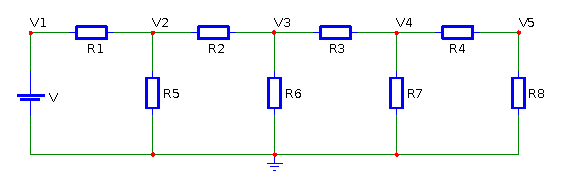
\includegraphics[width=12cm,angle=0]{./cap_linsis/pics/circuito_linear_8.eps}\label{circuitol8}
\end{center}

Complete a tabela abaixo representado a solução com 4 algarismos significativos:

\begin{center}
\begin{tabular}{|c|c|c|c|c|c|}
\hline
Caso & $V_1$ & $V_2$ & $V_3$ & $V_4$ & $V_5$\\
\hline
a & ~\hspace{40pt}~& ~\hspace{40pt}~& ~\hspace{40pt}~& ~\hspace{40pt}~& ~\hspace{40pt}~\\
\hline
b & & & & & \\
\hline
\end{tabular}
\end{center}

Então, refaça este problema reduzindo o sistema para apenas 4 incógnitas ($V_2$, $V_3$, $V_4$ e $V_5$).
\end{exer}
\ifisscilab
\begin{resp}
a)$V_5=98.44V$ b) $V_5=103.4V$

O problema com cinco incógnitas pode ser escrito na forma matricial conforme a seguir:
\begin{equation}\left[\begin{array}{ccccc}
1&0&0&0&0\\[.5cm]
\frac{1}{R_1}&-\left(\frac{1}{R_1}+\frac{1}{R_2}+\frac{1}{R_5}\right)&\frac{1}{R_2}&0&0\\[.5cm]
0&\frac{1}{R_2}&-\left(\frac{1}{R_2}+\frac{1}{R_3}+\frac{1}{R_6}\right)&\frac{1}{R_3}&0\\[.5cm]
0&0&\frac{1}{R_3}&-\left(\frac{1}{R_3}+\frac{1}{R_4}+\frac{1}{R_7}\right)&\frac{1}{R_4}\\[.5cm]
0&0&0&\frac{1}{R_4}&-\left(\frac{1}{R_4}+\frac{1}{R_8}\right)
\end{array}
\right]
\left[\begin{array}{c}
V_1\\[.65cm]
V_2\\[.65cm]
V_3\\[.65cm]
v_4\\[.65cm]
V_5
\end{array}
\right]=
\left[\begin{array}{c}
V\\[.65cm]
0\\[.65cm]
0\\[.65cm]
0\\[.65cm]
0
\end{array}
\right] \end{equation}
Este problema pode ser implementado no \verb+Scilab+ (para o item a) com o seguinte código:
\begin{verbatim}
R1=2, R2=2, R3=2, R4=2, R5=100, R6=100, R7=100, R8=50, V=127

A=[1      0                  0                  0                 0;
   1/R1  -(1/R1+1/R2+1/R5)   1/R2               0                 0;
   0      1/R2              -(1/R2+1/R3+1/R6)   1/R3              0;
   0      0                  1/R3             -(1/R3+1/R4+1/R7)   1/R4;
   0      0                  0                  1/R4             -(1/R4+1/R8)]
v=[V; 0; 0; 0; 0]
y=A\v
\end{verbatim}
O problema com quatro incógnitas pode ser escrito na forma matricial conforme a seguir:
\begin{equation}\left[\begin{array}{cccc}
-\left(\frac{1}{R_1}+\frac{1}{R_2}+\frac{1}{R_5}\right)&\frac{1}{R_2}&0&0\\[.5cm]
\frac{1}{R_2}&-\left(\frac{1}{R_2}+\frac{1}{R_3}+\frac{1}{R_6}\right)&\frac{1}{R_3}&0\\[.5cm]
0&\frac{1}{R_3}&-\left(\frac{1}{R_3}+\frac{1}{R_4}+\frac{1}{R_7}\right)&\frac{1}{R_4}\\[.5cm]
0&0&\frac{1}{R_4}&-\left(\frac{1}{R_4}+\frac{1}{R_8}\right)
\end{array}
\right]
\left[\begin{array}{c}
V_2\\[.65cm]
V_3\\[.65cm]
v_4\\[.65cm]
V_5
\end{array}
\right]=
\left[\begin{array}{c}
-\frac{V}{R1}\\[.65cm]
0\\[.65cm]
0\\[.65cm]
0
\end{array}
\right] \end{equation}
Cuja implementação pode ser feita conforme
\begin{verbatim}
A=[  -(1/R1+1/R2+1/R5)    1/R2               0                 0;
       1/R2              -(1/R2+1/R3+1/R6)   1/R3              0;
       0                  1/R3             -(1/R3+1/R4+1/R7)   1/R4;
       0                  0                  1/R4             -(1/R4+1/R8)]

v=[-V/R1; 0; 0; 0]
y=A\v
\end{verbatim}
\end{resp}
\fi

\begin{exer} Resolva o Problema~\ref{prob_circuito_resistores} pelos métodos de Jacobi e Gauss-Seidel.
\end{exer}


\begin{exer}(Interpolação) Resolva os seguintes problemas:
\begin{itemize}
\item[a)] Encontre o polinômio $P(x)=ax^2+bx+c$ que passa pelos pontos $(-1,-3)$, $(1,-1)$ e $(2,9)$.
\item[b)] Encontre os coeficientes $A$ e $B$ da função $f(x)=A\sin(x)+B\cos(x)$ tais que $f(1)=1.4$ e $f(2)=2.8$.
\item[c)] Encontre a função $g(x)=A_1\sin(x)+B_1\cos(x) + A_2\sin(2x)+B_2\cos(2x)$ tais que $f(1)=1$, $f(2)=2$, $f(3)=3$ e $f(4)=4$.
\end{itemize}
\end{exer}
\begin{resp}
Dica: $P(-1)=-3$, $P(1)=-1$ e $P(2)=9$ produzem três equações lineares para os coeficientes $a$, $b$ e $c$.
Resp: a) $P(x)=3x^2+x-5$, b) $A\approx 2.49$ e $B\approx -1.29$ c)$A_1\approx 1.2872058$, $A_2\approx - 4.3033034$, $B_1\approx 2.051533$ e $B_2\approx - 0.9046921$.
\end{resp}

%Este trabalho está licenciado sob a Licença Creative Commons Atribuição-CompartilhaIgual 3.0 Não Adaptada. Para ver uma cópia desta licença, visite https://creativecommons.org/licenses/by-sa/3.0/ ou envie uma carta para Creative Commons, PO Box 1866, Mountain View, CA 94042, USA.

%\documentclass[main.tex]{subfiles}
%\begin{document}

\chapter{Solução de sistemas de equações não lineares}\index{sistema de equações!não lineares}
Neste capítulo, estudaremos o método de Newton aplicado à resolução de sistemas não lineares de equações.

O método de Newton aplicado a encontrar a raiz $x^*$ da função $y=f(x)$ estudado na Seção~\ref{sec:metodo_newton_1d} consiste em um processo iterativo. Em cada passo deste processo, dispomos de uma aproximação $x^{(k)}$ para $x^*$ e construímos uma nova aproximação $x^{(k+1)}$.  Cada passo do método de Newton envolve os seguintes procedimentos:
\begin{itemize}
\item Linearização da função $f(x)$ no ponto $x^{(k)}$:
  \begin{equation}
    f(x)= f(x^{(k)})+ (x-x^{(k)}) f'(x^{(k)}) + O\left(|x-x^{(k)}|^2\right)
  \end{equation}
\item A aproximação $x^{(k+1)}$ é definida como o valor de $x$ em que a linearização $f(x^{(k)})+ (x-x^{(k)}) f'(x^{(k)})$ passa por zero.
\end{itemize}

%{\bf Observação:} $y=f(x^{(k)})+ (x-x^{(k)}) f'(x^{(k)})$ é a equação da reta que tangencia a curva $y=f(x)$ no ponto $(x^{(k)},f(x^{(k)}))$.

Queremos, agora, generalizar o método de Newton a fim de resolver problemas de várias equações e várias incógnitas, ou seja, encontrar $x_1,x_2,\ldots x_n$ que satisfazem as seguintes equações:

\begin{eqnarray}
f_1(x_1,x_2,\ldots,x_n)&=&0\\
f_2(x_1,x_2,\ldots,x_n)&=&0\\
&\vdots&\\
f_n(x_1,x_2,\ldots,x_n)&=&0
\end{eqnarray}

Podemos escrever este problema na forma vetorial definindo o vetor $x=[x_1,x_2,\ldots,x_n]^T$ e a função vetorial
\begin{equation}F(x)=\left[
\begin{array}{c}
f_1(x_1,x_2,\ldots,x_n)\\
f_2(x_1,x_2,\ldots,x_n)\\
\vdots\\
f_n(x_1,x_2,\ldots,x_n)
\end{array}
\right].\end{equation}

\begin{ex} Suponha que queiramos resolver numericamente o seguinte sistema de duas equações e duas incógnitas:
\begin{eqnarray}
\frac{x_1^2}{3}+x_2^2&=&1\\
x_1^2+\frac{x_2^2}{4}&=&1
\end{eqnarray}
Então definimos

\begin{equation}F(x)=\left[
\begin{array}{c}
\frac{x_1^2}{3}+x_2^2-1\\~\\
x_1^2+\frac{x_2^2}{4}-1
\end{array}
\right]\end{equation}
\end{ex}
Neste momento, dispomos de um problema na forma $F(x)=0$ e precisamos desenvolver uma técnica para linearizar a função $F(x)$. Para tal, precisamos de alguns conceitos do cálculo de várias variáveis.

Observe que $F(x)-F(x^{(0)})$ pode ser escrito como

\begin{equation}F(x)-F(x^{(0)})=\left[
\begin{array}{c}
f_1(x_1,x_2,\ldots,x_n)-f_1(x_1^{(0)},x_2^{(0)},\ldots,x_n^{(0)})\\
f_2(x_1,x_2,\ldots,x_n)-f_2(x_1^{(0)},x_2^{(0)},\ldots,x_n^{(0)})\\
\vdots\\
f_n(x_1,x_2,\ldots,x_n)-f_n(x_1^{(0)},x_2^{(0)},\ldots,x_n^{(0)})
\end{array}
\right]\end{equation}

Usamos a regra da cadeia
\begin{equation} df_i = \frac{\partial f_i}{\partial x_1} dx_1+\frac{\partial f_i}{\partial x_2} dx_2+\cdots + \frac{\partial f_i}{\partial x_n} dx_n=\sum_{j=1}^n\frac{\partial f_i}{\partial x_j} dx_j \end{equation}
e aproximamos as diferenças por derivadas parciais:
\begin{equation}  f_i(x_1,x_2,\ldots,x_n)-f_i(x_1^{(0)},x_2^{(0)},\ldots,x_n^{(0)})\approx \sum_{j=1}^n \frac{\partial f_i}{\partial x_j}\left(x_j-x_j^{(0)}\right) \end{equation}
Portanto,
\begin{equation}\label{eq_approx_newton}F(x)-F(x^{(0)})\approx \left[
\begin{array}{ccccc}
\frac{\partial f_1}{\partial x_1}&\frac{\partial f_1}{\partial x_2}&\cdots&\frac{\partial f_1}{\partial x_n}\\~\\
\frac{\partial f_2}{\partial x_1}&\frac{\partial f_2}{\partial x_2}&\cdots&\frac{\partial f_2}{\partial x_n}\\~\\
\vdots&\vdots&\ddots&\vdots\\~\\
\frac{\partial f_n}{\partial x_1}&\frac{\partial f_n}{\partial x_2}&\cdots&\frac{\partial f_n}{\partial x_n}\\~\\
\end{array}
\right]\left[
\begin{array}{c}
x_1-x_1^{(0)}\\~~\\
x_2-x_2^{(0)}\\~~\\
\vdots\\~~\\
x_n-x_n^{(0)}
\end{array}
\right],
\end{equation}

Definimos, então, a matriz jacobiana por\index{matrix!jacobiana}
\begin{equation}J_F= \frac{\partial(f_1,f_2,\ldots,f_n)}{\partial(x_1,x_2,\ldots,x_n)}=\left[
\begin{array}{ccccc}
\frac{\partial f_1}{\partial x_1}&\frac{\partial f_1}{\partial x_2}&\cdots&\frac{\partial f_1}{\partial x_n}\\~\\
\frac{\partial f_2}{\partial x_1}&\frac{\partial f_2}{\partial x_2}&\cdots&\frac{\partial f_2}{\partial x_n}\\~\\
\vdots&\vdots&\ddots&\vdots\\~\\
\frac{\partial f_n}{\partial x_1}&\frac{\partial f_n}{\partial x_2}&\cdots&\frac{\partial f_n}{\partial x_n}\\~\\
\end{array}
\right].
\end{equation}
Isto é, a matriz jacobiana de uma função ou simplesmente, o jacobiano de uma função $F(x)$ é a matriz formada pelas suas derivadas parciais:
\begin{equation} \left(J_F\right)_{ij}=\frac{\partial f_i}{\partial x_j}. \end{equation}

Nestes termos, podemos reescrever \eqref{eq_approx_newton} como
\begin{equation} F(x)\approx F(x^{(0)}) + J_F(x^{(0)}) (x-x^{(0)}) \end{equation}
Esta expressão é chamada de linearização de $F(x)$ no ponto $x^{(0)}$ e generaliza a linearização em uma dimensão dada por $f(x)\approx f(x^{(0)})+f'(x^{(0)}) (x-x^{(0)})$.

%%%%%%%%%%%%%%%%%%%%
% python
%%%%%%%%%%%%%%%%%%%%
\ifispython
Ao longo deste capítulo, assumiremos que as seguintes bibliotecas e módulos \verb+Python+ estão importadas:
\begin{verbatim}
import numpy as np
from numpy import linalg
\end{verbatim}
\fi
%%%%%%%%%%%%%%%%%%%%

\section{Método de  Newton para sistemas}\index{método de Newton!para sistemas}

Nesta seção, construiremos o método de Newton ou Newton-Raphson generalizado para sistemas. Assumimos, portanto, que a função $F(x)$ é diferenciável e que existe um ponto $x^*$ tal que $F(x^*)=0$. Seja $x^{(k)}$ uma aproximação para $x^*$, queremos construir uma nova aproximação $x^{(k+1)}$ através da linearização de $F(x)$ no ponto $x^{(k)}$.

\begin{itemize}
\item Linearização da função $F(x)$ no ponto $x^{(k)}$:
  \begin{equation}
F(x)= F(x^{(k)})+ J_F\left(x^{(k)}\right) \left(x-x^{(k)}\right)  + O\left(\|x-x^{(k)}\|^2\right)
  \end{equation}
\item A aproximação $x^{(k)}$ é definida como o ponto $x$ em que a linearização $F(x^{(k)})+ J_F\left(x^{(k)}\right) \left(x-x^{(k)}\right)$ é nula, ou seja:
\begin{equation} F(x^{(k)})+ J_F\left(x^{(k)}\right) \left(x^{(k+1)}-x^{(k)}\right)=0 \end{equation}
\end{itemize}

Supondo que a matriz jacobina seja inversível no ponto $x^{(k)}$, temos:
\begin{eqnarray}
J_F\left(x^{(k)}\right) \left(x^{(k+1)}-x^{(k)}\right)&=&-F(x^{(k)})\\
x^{(k+1)}-x^{(k)}&=&-J_F^{-1}\left(x^{(k)}\right)F(x^{(k)})\\
x^{(k+1)}&=&x^{(k)}-J_F^{-1}\left(x^{(k)}\right)F(x^{(k)})
\end{eqnarray}

Desta forma, o método iterativo de Newton-Raphson para encontrar as raízes de $F(x)=0$ é dado por:
\begin{equation}
\left\{\begin{array}{rcl}
x^{(k+1)} &=& x^{(k)}-J_F^{-1}\left(x^{(k)}\right)F(x^{(k)}),~~ k> 0\\
x^{(0)}&=&\text{dado inicial}
\end{array}\right.
\end{equation}

\begin{obs} Usamos subíndices para indicar o elemento de um vetor e superíndices para indicar o passo da iteração. Assim, $x^{(k)}$ se refere à iteração $k$ e $x_i^{(k)}$ se refere à componente $i$ no vetor $x^{(k)}$.
\end{obs}
\begin{obs} A notação $J_F^{-1}\left(x^{(k)}\right)$ enfatiza que a jacobiana deve ser calculada a cada passo.
\end{obs}
\begin{obs} Podemos definir o passo $\Delta^{(k)}$ como
\begin{equation} \Delta^{(k)}= x^{(k+1)}-x^{(k)} \end{equation}
Assim, $\Delta^{(k)}=-J_F^{-1}\left(x^{(k)}\right)F(x^{(k)})$, ou seja, $\Delta^{(k)}$ resolve o problema linear:
\begin{equation} J_F\left(x^{(k)}\right)\Delta^{(k)}= - F(x^{(k)}) \end{equation}
Em geral, é menos custoso resolver o sistema acima do que calcular o inverso da jacobiana e multiplicar pelo vetor $F(x^{(k)})$.
\end{obs}

\begin{ex} Retornamos ao nosso exemplo inicial, isto é, resolver numericamente o seguinte sistema não linear:
\begin{eqnarray}
\frac{x_1^2}{3}+x_2^2&=&1\\
x_1^2+\frac{x_2^2}{4}&=&1
\end{eqnarray}
Para tal, definimos a função $F(x)$:
\begin{equation}
  F(x)=\left[
\begin{array}{c}
\displaystyle \frac{x_1^2}{3}+x_2^2-1\\
\displaystyle x_1^2+\frac{x_2^2}{4}-1
\end{array}
\right]
\end{equation}
cuja jacobiana é:
\begin{equation}
  J_F=\left[\begin{array}{cc}
      \displaystyle \frac{2x_1}{3} & 2x_2\\
      \displaystyle 2x_1&\frac{x_2}{2}
    \end{array}\right]
\end{equation}

%%%%%%%%%%%%%%%%%%%%
% scilab
%%%%%%%%%%%%%%%%%%%%
\ifisscilab
Faremos a implementação numérica no \verb+Scilab+. Para tal definimos as funções que implementarão $F(x)$ e a $J_F(x)$
\begin{verbatim}
function y=F(x)
    y(1)=x(1)^2/3+x(2)^2-1
    y(2)=x(1)^2+x(2)^2/4-1
endfunction

function y=JF(x)
    y(1,1)=2*x(1)/3
    y(1,2)=2*x(2)
    y(2,1)=2*x(1)
    y(2,2)=x(2)/2
endfunction
\end{verbatim}
Alternativamente, estas funções poderiam ser escritas como
\begin{verbatim}
function y=F(x)
    y=[x(1)^2/3+x(2)^2-1; x(1)^2+x(2)^2/4-1]
endfunction

function y=JF(x)
    y=[2*x(1)/3  2*x(2); 2*x(1) x(2)/2]
endfunction
\end{verbatim}
Desta forma, se $x$ é uma aproximação para a raiz, pode-se calcular a próxima aproximação através dos comandos:
\begin{verbatim}
delta=-JF(x)\F(x)
x=x+delta
\end{verbatim}
Ou simplesmente
\begin{verbatim}
x=x-JF(x)\F(x)
\end{verbatim}
\fi
%%%%%%%%%%%%%%%%%%%%
%%%%%%%%%%%%%%%%%%%%
% octave
%%%%%%%%%%%%%%%%%%%%
\ifisoctave
Faremos a implementação numérica no \verb+GNU Octave+. Para tal definimos as funções que implementarão $F(x)$ e a $J_F(x)$
\begin{verbatim}
function y=F(x)
    y(1)=x(1)^2/3+x(2)^2-1
    y(2)=x(1)^2+x(2)^2/4-1
endfunction

function y=JF(x)
    y(1,1)=2*x(1)/3
    y(1,2)=2*x(2)
    y(2,1)=2*x(1)
    y(2,2)=x(2)/2
endfunction
\end{verbatim}
Alternativamente, estas funções poderiam ser escritas como
\begin{verbatim}
function y=F(x)
    y=[x(1)^2/3+x(2)^2-1; x(1)^2+x(2)^2/4-1]
endfunction

function y=JF(x)
    y=[2*x(1)/3  2*x(2); 2*x(1) x(2)/2]
endfunction
\end{verbatim}
Desta forma, se $x$ é uma aproximação para a raiz, pode-se calcular a próxima aproximação através dos comandos:
\begin{verbatim}
delta=-JF(x)\F(x)
x=x+delta
\end{verbatim}
Ou simplesmente
\begin{verbatim}
x=x-JF(x)\F(x)
\end{verbatim}
\fi
%%%%%%%%%%%%%%%%%%%%
%%%%%%%%%%%%%%%%%%%%
% python
%%%%%%%%%%%%%%%%%%%%
\ifispython
Faremos a implementação numérica em \verb+Python+. Para tal definimos as funções que implementarão $F(x)$ e a $J_F(x)$
\begin{verbatim}
>>> def F(x):
...     y = np.zeros(2)
...     y[0] = x[0]**2/3 + x[1]**2 - 1
...     y[1] = x[0]**2 + x[1]**2/4 - 1
...     return y
...
>>> def JF(x):
...     y = np.zeros((2,2))
...     y[0,0] = 2*x[0]/3
...     y[0,1] = 2*x[1]
...     y[1,0] = 2*x[0]
...     y[1,1] = x[1]/2
...     return y
...
\end{verbatim}
Desta forma, se $x$ é uma aproximação para a raiz, pode-se calcular a próxima aproximação através dos comandos:
\begin{verbatim}
>>> delta = -np.linalg.inv(JF(x)).dot(F(x))
>>> x = x + delta
\end{verbatim}
Ou simplesmente
\begin{verbatim}
>>> x = x - np.linalg.inv(JF(x)).dot(F(x))
\end{verbatim}
\fi
%%%%%%%%%%%%%%%%%%%%
Observe que as soluções exatas desse sistema são $\left(\pm \sqrt{\frac{9}{11}},\pm \sqrt{\frac{8}{11}}\right)$.
\end{ex}


\begin{ex} Encontre uma aproximação para a solução do sistema
\begin{eqnarray}
x_1^2=\cos(x_1x_2)+1\\
\sin(x_2)=2\cos(x_1)
\end{eqnarray}
que fica próxima ao ponto $x_1=1,5$ e $x_2=0,5$.
\end{ex}
\begin{sol} Vamos, aqui, dar as principais ideias para obter a solução usando o método de Newton.
Começamos definindo nossa aproximação inicial por $x^{(1)} = (1,5, 0,5)$. Então iteramos:
\begin{equation}
  x^{(n+1)} = x^{(n)} - J_F^{-1}(x)F(x), \quad n\geq 1.
\end{equation}
onde
  \begin{equation}
    F(x)=\left[\begin{array}{c}
        \displaystyle x_1^2-\cos(x_1x_2)-1\\
        \displaystyle \sin(x_2)-2\cos(x_1)
      \end{array}\right]
  \end{equation}
e sua jacobiana é
\begin{equation}
  J_F(x) = \left[\begin{array}{cc}
    \displaystyle 2x_1 +x_2\sin(x_1x_2) & x_1\sin(x_1x_2)\\
    \displaystyle 2\sin(x_1) & \cos(x_2)
  \end{array}\right]
\end{equation}
As iterações convergem para $x = (1,3468109,~0,4603195)$.

%%%%%%%%%%%%%%%%%%%%
% scilab
%%%%%%%%%%%%%%%%%%%%
\ifisscilab
No \verb+Scilab+, podemos implementá-las com o seguinte código:
\begin{verbatim}
function y=F(x)
    y(1) = x(1)^2-cos(x(1)*x(2))-1
    y(2) = sin(x(2))-2*cos(x(1))
endfunction

function y=JF(x)
    y(1,1) = 2*x(1)+x(2)*sin(x(1)*x(2))
    y(1,2) = x(1)*sin(x(1)*x(2))

    y(2,1) = 2*sin(x(1))
    y(2,2) = cos(x(2))
endfunction
\end{verbatim}

E agora, basta iterar:
\begin{verbatim}
x=[1.5; .5]
x=x-JF(x)\F(x) //(5 vezes)
\end{verbatim}
\fi
%%%%%%%%%%%%%%%%%%%%
%%%%%%%%%%%%%%%%%%%%
% octave
%%%%%%%%%%%%%%%%%%%%
\ifisoctave
No \verb+GNU Octave+, podemos implementá-las com o seguinte código:
\begin{verbatim}
function y=F(x)
    y(1) = x(1)^2-cos(x(1)*x(2))-1
    y(2) = sin(x(2))-2*cos(x(1))
endfunction

function y=JF(x)
    y(1,1) = 2*x(1)+x(2)*sin(x(1)*x(2))
    y(1,2) = x(1)*sin(x(1)*x(2))

    y(2,1) = 2*sin(x(1))
    y(2,2) = cos(x(2))
endfunction
\end{verbatim}

E agora, basta iterar:
\begin{verbatim}
x=[1.5; .5]
x=x-JF(x)\F(x) //(5 vezes)
\end{verbatim}
\fi
%%%%%%%%%%%%%%%%%%%%
%%%%%%%%%%%%%%%%%%%%
% python
%%%%%%%%%%%%%%%%%%%%
\ifispython
Em \verb+Python+, podemos implementá-las com o seguinte código:
\begin{verbatim}
def F(x):
    y = np.zeros(2)

    y[0] = x[0]**2 - np.cos(x[0]*x[1]) - 1
    y[1] = np.sin(x[1]) - 2*np.cos(x[0])

    return y

def JF(x):
    y = np.zeros((2,2))

    y[0,0] = 2*x[0] + x[1]*np.sin(x[0]*x[1])
    y[0,1] = x[0]*np.sin(x[0]*x[1])

    y[1,0] =  2*np.sin(x[0])
    y[1,1] = np.cos(x[1])

    return y
\end{verbatim}

E agora, basta iterar:
\begin{verbatim}
>>> x = np.array([1.5,0.5])
>>> x=x-np.linalg.inv(JF(x)).dot(F(x))
\end{verbatim}
\fi
%%%%%%%%%%%%%%%%%%%%
\end{sol}

%%%%%%%%%%%%%%%%%%%%
% scilab
%%%%%%%%%%%%%%%%%%%%
\ifisscilab
\subsection{Código Scilab: Newton para sistemas}

\verbatiminput{./cap_nlinsis/codes/scilab/metodo_de_newton/newton.sci}
\fi
%%%%%%%%%%%%%%%%%%%%
%%%%%%%%%%%%%%%%%%%%
% octave
%%%%%%%%%%%%%%%%%%%%
\ifisoctave
\subsection{Código GNU Octave: Newton para sistemas}

\verbatiminput{./cap_nlinsis/codes/octave/metodo_de_newton/newton.m}
\fi
%%%%%%%%%%%%%%%%%%%%
%%%%%%%%%%%%%%%%%%%%
% python
%%%%%%%%%%%%%%%%%%%%
\ifispython
\subsection{Código Python: Newton para Sistemas}

\verbatiminput{./cap_nlinsis/codes/python/metodo_de_newton/newton.py}
\fi
%%%%%%%%%%%%%%%%%%%%

\subsection*{Exercícios resolvidos}

\construirExeresol

\subsection*{Exercícios}

\begin{exer} Faça o que se pede:
\begin{itemize}
\item[a)] Encontre o gradiente da função \begin{equation} f(x,y)=x^2y+\cos(xy)-4 \end{equation}
\item[b)] Encontre a matriz jacobiana associada à função
\begin{equation} F(x,y)=\left[\begin{array}{c}x\cos(x)+y\\ e^{-2x+y}\end{array} \right]. \end{equation}
\item[c)] Encontre a matriz jacobiana associada à função
\begin{equation}L(x)=\left[\begin{array}{c}
a_{11}x_1 + a_{12}x_2 +a_{13}x_3-y_1\\
a_{21}x_1 + a_{22}x_2 +a_{23}x_3-y_2\\
a_{31}x_1 + a_{32}x_2 +a_{33}x_3-y_3
\end{array}
 \right].\end{equation}
\end{itemize}
\end{exer}
\begin{resp}
$\nabla f = [2xy-y\sin(xy), x^2-x\sin(xy)]^T$
\begin{equation}J_F=\left[\begin{array}{cc}
\cos(x)-x\sin(x) & 1\\
-2e^{-2x+y} &e^{-2x+y}
\end{array}
\right]\end{equation}
\begin{equation} \left(J_L\right)_{ij}=a_{ij} \end{equation}
\end{resp}

\begin{exer} Encontre uma aproximação numérica para o seguinte problema não linear de três equações e três incógnitas:
\begin{eqnarray}
2x_1-x_2&=&\cos(x_1)\\
-x_1+2x_2-x_3&=&\cos(x_2)\\
-x_2+	x_3&=&\cos(x_3)
\end{eqnarray}
Partindo das seguintes aproximações iniciais:
\begin{itemize}
\item[a)] $x^{(0)}=[1,~1,~1]^T$
\item[b)] $x^{(0)}=[-0,5,~-2,~-3]^T$
\item[c)] $x^{(0)}=[-2,~-3,~-4]^T$
\item[d)] $x^{(0)}=[0,~0,~0]^T$
\end{itemize}
\end{exer}
\begin{resp}
  \construirResp
\end{resp}


\begin{exer}\label{prob_para_elipse}
 Encontre os pontos de intersecção entre a parábola $y=x^2+1$ e a elipse $x^2+y^2/4=1$ seguindo os seguintes passos:
\begin{itemize}
\item[a)] Faça um esboço das duas curvas e entenda o problema. Verifique que existem dois pontos de intersecção, um no primeiro quadrante e outro no segundo quadrante do plano $xy$.
\item[b)] A partir de seu esboço, encontre aproximações para $x$ e $y$ em cada ponto.
\item[c)] Escreva o problema na forma $F\left(\left[\begin{array}{c}x\\y\end{array}\right]\right)=\left[\begin{array}{c}0\\0\end{array}\right]$
\item[d)] Encontre a jacobiana $J_F$.
\item[e)] Construa a iteração do método de Newton.
\item[f)] Implemente no computador.
\item[g)] Resolva o sistema analiticamente e compare as respostas.
\end{itemize}
\end{exer}
\begin{resp}
As curvas possuem dois pontos de intersecção. A posição exata destes pontos de intersecção é dada por $\left(\sqrt{2\sqrt{3}-3},2\sqrt{3}-2\right)$ e $\left(-\sqrt{2\sqrt{3}-3},2\sqrt{3}-2\right)$. Use a solução exata para comparar com a solução aproximada obtida.
\end{resp}

\begin{exer} Encontre os pontos de intersecção entre a parábola $y=x^2$ e a curva $y=\cos(x)$ seguindo os seguintes passos:
\begin{itemize}
\item[a]) Faça um esboço das duas curvas, entenda o problema. Verifique que existem dois pontos de intersecção, um no primeiro quadrante e outro no segundo quadrante do plano $xy$.
\item[b]) A partir de seu esboço, encontre aproximações para $x$ e $y$ em cada ponto.
\item[c]) Escreva o problema na forma $F\left(\left[\begin{array}{c}x\\y\end{array}\right]\right)=\left[\begin{array}{c}0\\0\end{array}\right]$
\item[d]) Encontre a jacobiana $J_F$.
\item[e]) Construa a iteração do método de Newton.
\item[f]) Implemente no \ifisscilab\verb+Scilab+\fi\ifispython\verb+Python+\fi\ifisoctave\verb+Octave+\fi.
\item[g]) Transforme o sistema em um problema de uma única variável e compare com a resposta do Problema~\ref{1d:cosx2}.
%\item[h]) Refaça o item e, usando a função {\it derivative()} para aproximar a matriz jacobiana.
\end{itemize}
\end{exer}
\begin{resp}
 $\left(\pm 0.8241323, 0.6791941\right)$
\end{resp}

\begin{exer} Encontre uma aproximação com erro inferior a $10^{-5}$ em cada incógnita para a solução próxima da origem do sistema
\begin{eqnarray}
6x-2y+e^{z}&=&2\\
\sin(x)-y+z&=&0\\
\sin(x)+2y+3z&=&1
\end{eqnarray}
\end{exer}
\begin{resp}
$x\approx 0,259751, y\approx  0,302736, z\approx  0,045896$
\end{resp}


\begin{exer}(Entenda casos particulares)
\begin{itemize}
\item Considere a função $L(x)=Ax-b$, onde $A$ é uma matriz $n\times n$ inversível e $b$ um vetor coluna em $\mathbb{R}^n$. O que acontece quando aplicamos o método de Newton para encontrar as raízes de $L(x)$?
\item Mostre que o método de Newton-Raphson aplicado a uma função diferenciável do tipo $f:\mathbb{R}\to\mathbb{R}$ se reduz ao método de Newton estudado na primeira área.
\end{itemize}
\end{exer}
\begin{resp}
  \construirResp
\end{resp}

\begin{exer}\label{prob_bitang}Considere a função $f(x)=\frac{\sin(x)}{x+1}$, encontre a equação da reta que tangencia dois pontos da curva $y=f(x)$ próximos ao primeiro e segundo ponto de máximo no primeiro quadrante, respectivamente. Veja a Figura~\ref{pic:bitang}.
\end{exer}
\begin{figure}
  \centering
  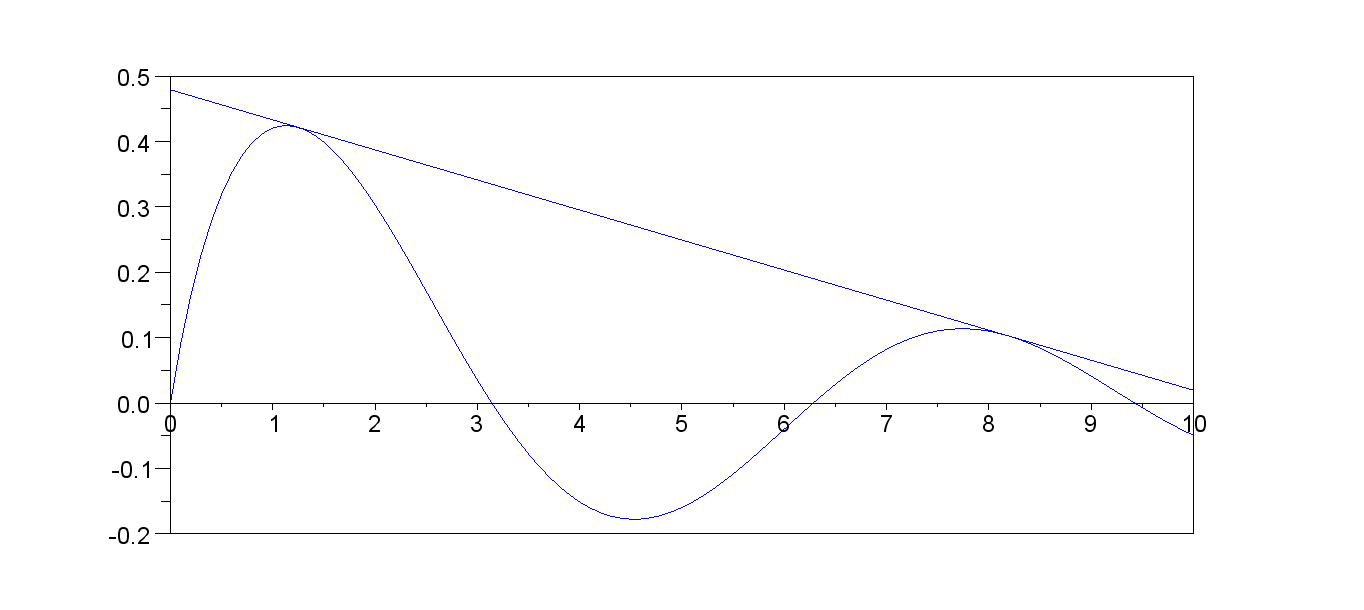
\includegraphics[width=\textwidth]{cap_nlinsis/pics/curva_Q23}
  \caption{Reta bitangente a uma curva.}
  \label{pic:bitang}
\end{figure}
\begin{resp}
  $y=mx+b$ com $m\approx - 0.0459710 $ e $b\approx 0.479237$
  Uma metodologia possível para resolver este problema é dada a seguir:

  Sejam $x_1$ e $x_2$ as abscissas dos dois pontos em que a reta tangencia a curva. A equação da reta bitangente assume a seguinte forma:
  \begin{equation} y=f(x_1) + m(x-x_1)  \end{equation}
  onde o coeficiente angular $m$ é dado por
  \begin{equation} m=\frac{f(x_2)-f(x_1)}{x_2-x_1} \end{equation}

  Da condição de tangência, temos que o coeficiente angular da reta, $m$, deve igual à derivada da função $f(x)$ nos dois pontos de tangência.
  \begin{equation} m=f'(x_1)=f'(x_2) \end{equation}
  E sabemos que:
  \begin{equation} f'(x)=\frac{\cos(x)}{1+x}-\frac{\sin(x)}{(1+x)^2}. \end{equation}

  Assim, podemos reescrever o problema como
  \begin{eqnarray}
\frac{\cos(x_1)}{1+x_1}-\frac{\sin(x_1)}{(1+x_1)^2}-\frac{\cos(x_2)}{1+x_2}+\frac{\sin(x_2)}{(1+x_2)^2}=0\\
\frac{\cos(x_1)}{1+x_1}-\frac{\sin(x_1)}{(1+x_1)^2}-\frac{f(x_2)-f(x_1)}{x_2-x_1}=0
\end{eqnarray}
Este é um sistema não linear de duas incógnitas.

Os valores iniciais para o método podem ser obtidos do gráfico buscando valores próximos aos dois primeiros pontos de máximos. Por exemplo: $x_1^{(0)}=1$ e $x_2^{(0)}=8$. Obtemos $x_1\approx 1,2464783$ e $x_2\approx 8,1782997$ e $m$ pode ser obtido através desses valores.
\end{resp}

\begin{figure}
        \centering
	    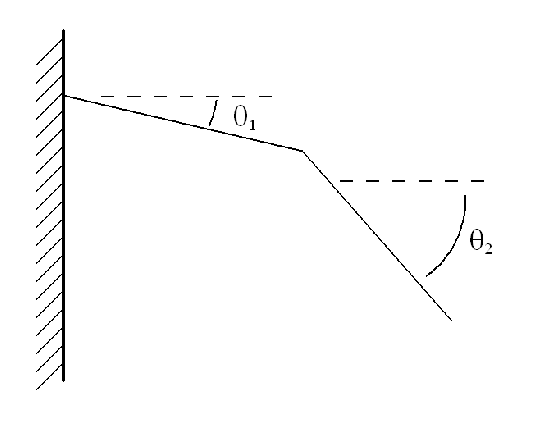
\includegraphics[width=.5\textwidth]{cap_nlinsis/pics/dois_segmentos}
		\caption{Sistema mecânico com dois segmentos.}
		\label{pic:dois_segmentos}
	\end{figure}

\begin{exer}{(Estática)}\label{prob:dois_segmentos} Considere o sistema mecânico constituído de dois segmentos de mesmo comprimento $L$ presos entre si e a uma parede por articulações conforme a Figura~\ref{pic:dois_segmentos}.

O momento em cada articulação é proporcional à deflexão com constante de proporcionalidade $k$. Os segmentos são feitos de material homogêneo de peso $P$. A condição de equilíbrio pode ser expressa em termos dos ângulos $\theta_1$ e $\theta_2$ conforme:
\begin{eqnarray}
k\theta_1&=& \frac{3PL}{2}\cos\theta_1 + k\left(\theta_2-\theta_1\right)\\
k\left(\theta_2-\theta_1\right)&=& \frac{PL}{2}\cos\theta_2
\end{eqnarray}
Considere $P=100N$, $L=1m$ e calcule os ângulos $\theta_1$ e $\theta_2$ quando:
\begin{itemize}
\item[a)] $k=1000$ Nm/rad
\item[b)] $k=500$ Nm/rad
\item[c)] $k=100$ Nm/rad
\item[d)] $k=10$ Nm/rad
\end{itemize}
\noindent {\bf Obs:}Você deve escolher valores para iniciar o método. Como você interpretaria fisicamente a solução para produzir palpites iniciais satisfatórios? O que se altera entre o caso a e o caso d?
\end{exer}
\begin{resp}
$\left(0.1956550;0.2441719 \right)$, $\left(0.3694093;0.4590564\right) $, $\left( 0.9990712;1.1865168  \right)$ e $\left(1.4773606;1.5552232 \right)$
\end{resp}


\begin{exer}{(estática - problemas de três variáveis)} Considere, agora, o sistema mecânico semelhante ao do Problema~\ref{prob:dois_segmentos}, porém constituído de três segmentos de mesmo comprimento $L$ presos entre si e a uma parede por articulações.

O momento em cada articulação é proporcional à deflexão com constante de proporcionalidade $k$. Os segmentos são feitos de material homogêneo de peso $P$. A condição de equilíbrio pode ser expressa em termos dos ângulos $\theta_1$, $\theta_2$ e $\theta_3$ conforme:
\begin{eqnarray}
k\theta_1&=& \frac{5PL}{2}\cos\theta_1 + k\left(\theta_2-\theta_1\right)\\
k\left(\theta_2-\theta_1\right)&=& \frac{3PL}{2}\cos\theta_2+k\left(\theta_3-\theta_2\right)\\
k\left(\theta_3-\theta_2\right)&=& \frac{PL}{2}\cos\theta_3
\end{eqnarray}
Considere $P=10$N, $L=1$m e calcule os ângulos $\theta_1$, $\theta_2$ e $\theta_3$ quando:
\begin{itemize}
\item[a)] $k=1000$Nm/rad
\item[b)] $k=100$Nm/rad
\item[c)] $k=10$Nm/rad
\end{itemize}
\end{exer}
\begin{resp}
$\left(0.0449310; 0.0648872; 0.0698750  \right)$, $\left(0.3981385; 0.5658310; 0.6069019  \right)$, \\
$\left(1.1862966;1.4348545;1.480127  \right)$
\end{resp}

\begin{figure}
        \centering
	    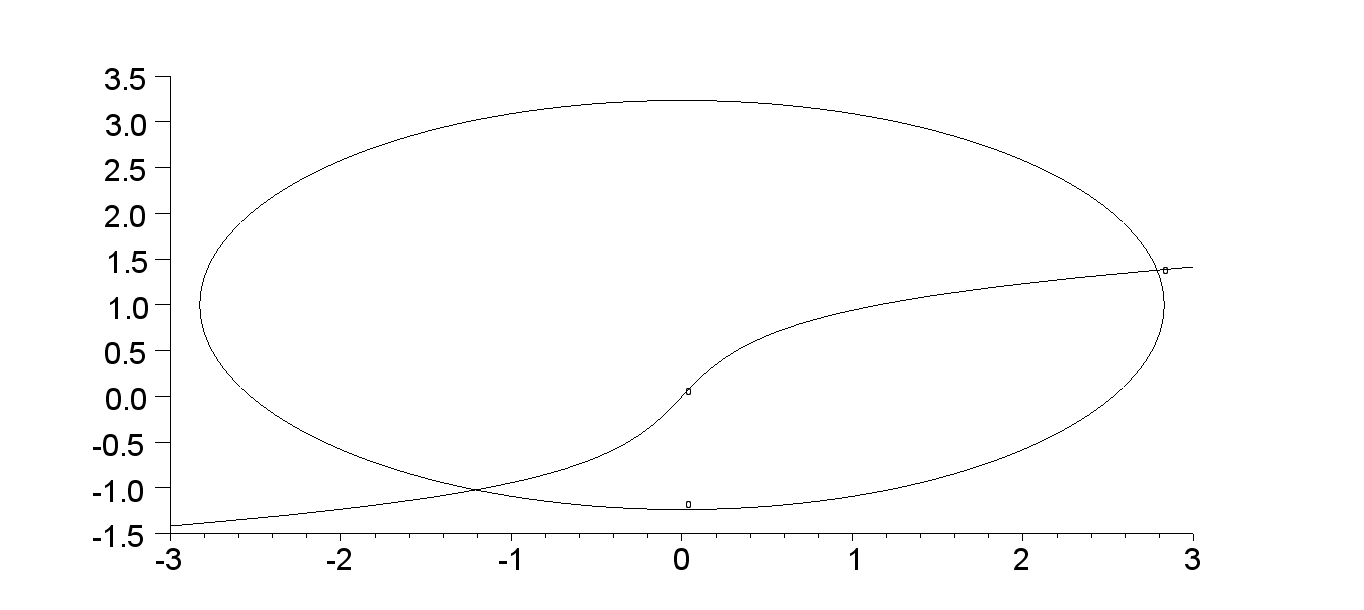
\includegraphics[width=.5\textwidth]{cap_nlinsis/pics/inter_curvas}
		\caption{intersecção entre duas curvas.}
		\label{pic:inter_curvas}
	\end{figure}

\begin{exer}  Considere o problema de encontrar os pontos de intersecção das curvas descritas por (ver Figura~\ref{pic:inter_curvas}):
\begin{eqnarray}
\frac{x^2}{8}+\frac{(y-1)^2}{5}&=&1\\~\\
\tan^{-1}(x)+x&=&y+y^3
\end{eqnarray}
 Com base no gráfico, encontre soluções aproximadas para o problema e use-as para iniciar o método de Newton-Raphson. Encontre as raízes com erro inferior a $10^{-5}$.
\end{exer}
\begin{resp}
$\left(-1,2085435, -1,0216674 \right)$ e $\left(2,7871115, 1,3807962\right)$

\ifisscilab
Exemplo de implementação:
\begin{verbatim}
function z=f(x,y)
    z=x^2/8+(y-1)^2/5-1
endfunction
function z=g(x,y)
    z=atan(x)+x-y-y^3
endfunction

contour([-3:.1:3],[-2:.1:4],f,[0 0])
contour([-3:.1:3],[-2:.1:4],g,[0 0])

function y=F(x)
    y(1)=f(x(1),x(2))
    y(2)=g(x(1),x(2))
endfunction
function y=JF(x)
    y(1,1)=x(1)/4
    y(1,2)=2*(x(2)-1)/5
    y(2,1)=1/(1+x(1)^2)+1
    y(2,2)=-1-3*x(2)^2
endfunction

//primeiro ponto
//x=[-1.2;-1.0]

//segundo ponto
//x=[2.8;1.4]

x=x-JF(x)\F(x)   // 4 vezes
\end{verbatim}
\fi
\end{resp}


\begin{exer} Considere o sistema de equações dado por
\begin{eqnarray}
\frac{(x-3)^2}{16}+\frac{(y-1)^2}{36}&=&1\\
\tanh(x)+x&=&2\sin y-0.01y^3
\end{eqnarray}
Usando procedimentos analíticos, determine uma região limitada do plano onde se encontram necessariamente todas as raízes do problema.
Encontre as raízes desse sistema com pelo menos quatro dígitos significativos corretos usando o método de Newton. Você deve construir o método de Newton indicando as funções envolvidas e calculando a matriz jacobiana analiticamente. Use que $\frac{d}{du}\tanh u = 1-\tanh^2u$, se precisar.
\end{exer}
\begin{resp}
 A primeira curva trata-se de uma elipse de centro $(3,1)$ e semi-eixos 4 e 6, portanto seus pontos estão contidos no retângulo $-1\leq x \leq 7$ e $-5\leq y \leq 7$.

As soluções são $\left( -0,5384844 , -1,7978634\right)$ e $\left(2,8441544, 6,9954443\right)$.

\ifisscilab
Uma possível implementação é
\begin{verbatim}

function z=f(x,y)
    z=(x-3)^2/16+(y-1)^2/36-1
endfunction

function z=g(x,y)
    z=atan(x)+x-sin(y)-0.01*y^3
endfunction

contour([-1:.1:7],[-5:.1:7],f,[0 0])
contour([-1:.1:7],[-5:.1:7],g,[0 0])

function y=F(x)
    y(1)=f(x(1),x(2))
    y(2)=g(x(1),x(2))
endfunction
function y=JF(x)
    y(1,1)=(x(1)-3)/8
    y(1,2)=(x(2)-1)/18
    y(2,1)=1/(1+x(1)^2)+1
    y(2,2)=-cos(x(2))-0.03*x(2)^2
endfunction 


//primeiro ponto
//x=[-.5;-2.0]

//segundo ponto
//x=[3;7]

x=x-JF(x)\F(x)   // 4 vezes
\end{verbatim}
\fi
\end{resp}


\begin{exer}(Otimização)\label{nlinsis:usinas} Uma indústria consome energia elétrica de três usinas fornecedoras. O custo de fornecimento em reais por hora como função da potência consumida em kW é dada pelas seguintes funções
\begin{eqnarray}
C_1(x)&=&10+.3x+10^{-4}x^2+3.4\cdot 10^{-9}x^4\\
C_2(x)&=&50+.25x+2\cdot 10^{-4}x^2+4.3\cdot 10^{-7}x^3\\
C_3(x)&=&500+.19x+5\cdot 10^{-4}x^2+1.1\cdot 10^{-7}x^4
\end{eqnarray}
Calcule a distribuição de consumo que produz custo mínimo quando a potência total consumida é $1500kW$. Dica: Denote por $x_1$, $x_2$ e $x_3$ as potências consumidas das usinas 1, 2 e 3, respectivamente.  O custo total será dado por $C(x_1,x_2,x_3)=C_1(x_1)+C_2(x_2)+C_3(x_3)$ enquanto o consumo total é $x_1+x_2+x_3=1500$. Isto é, queremos minimizar a função custo total dada por:
\begin{equation} C(x_1,x_2,x_3)=C_1(x_1)+C_2(x_2)+C_3(x_3) \end{equation}
restrita à condição
\begin{equation} G(x_1,x_2,x_3)=x_1+x_2+x_3-1500=0. \end{equation}
Pelos multiplicadores de Lagrange, temos que resolver o sistema dado por:
\begin{eqnarray}
\nabla C(x_1,x_2,x_3) &=& \lambda \nabla G(x_1,x_2,x_3)\\
G(x_1,x_2,x_3)&=&0
\end{eqnarray}
\end{exer}
\begin{resp}
 $(x_1,x_2,x_3)\approx (453,62,~ 901,94,~ 144,43)$
\end{resp}


\begin{exer} \label{nlinsis:prob_ajuste_eax} Encontre a função do tipo $f(x)=Ab^{x}$ que melhor aproxima os pontos $(0,~3,1)$, $(1,~4,4)$ e $(2,~6,7)$ pelo critério dos mínimos quadrados. Dica: Você deve encontrar os valores de $A$ e $b$ que minimizam o resíduo dado por
\begin{equation} R=\left[3,1-f(0)\right]^2+\left[4,4-f(1)\right]^2+\left[6,7-f(2)\right]^2. \end{equation}
{\bf Dica:} Para construir aproximações para resposta e iniciar o método, considere a função $f(x)=Ab^x$ que passa pelo primeiro e terceiro ponto.
\end{exer}
\begin{resp}
Inicialização do método: $A^{(0)}= 3,1$ e $b^{(0)}= \sqrt{\frac{6,7}{3,1}}$
$A\approx  3.0297384 $ e $b\approx 1.4835346$.
\end{resp}


\begin{exer}Encontre o valor máximo da função \begin{equation} f(x,y)=-x^4-y^6+3xy^3-x \end{equation} na região $(x,y)\in [-2,0]\times [-2,0]$
 seguindo os seguintes passos:
\begin{itemize}
  \item[a)] Defina a função $z=f(x,y)=-x^4-y^6+3xy^3-x$ e trace o gráfico de contorno na região.
  \item[b)] Com base no gráfico, encontre valores aproximados para as coordenadas $xy$ do ponto de máximo.
  \item[c)] Sabendo que o ponto de máximo acontece quando o gradiente é nulo, escreva o problema como um sistema de duas equações não lineares e duas incógnitas.
  \item[d)] Implemente o método de Newton.
\end{itemize}
\end{exer}
 \begin{resp}
 $f(-1,1579702, -1,2020694)\approx 2.376985$

\ifisscilab
Um exemplo de implementação no Scilab é:
\begin{verbatim}
deff('z=f(x,y)','z=-x^4-y^6+3*x*y^3-x')
contour([-2:.01:0],[-2:.01:0],f,[ 0:.2: 3])
deff('z=F(x)','z=[-4*x(1)^3+3*x(2)^3-1;-6*x(2)^5+9*x(1)*x(2)^2]')
deff('z=JF(x)','z=[-12*x(1)^2,9*x(2)^2;9*x(2)^2,-30*x(2)^4+18*x(1)*x(2)]')
x=[-1.2;-1.2]
x=x-JF(x)\F(x)
x=x-JF(x)\F(x)
x=x-JF(x)\F(x)
x=x-JF(x)\F(x)
mprintf('f(%f,%f)=%f',x(1),x(2),f(x(1),x(2)))
\end{verbatim}
\fi
\end{resp}

\begin{exer}A função $f(x,y,z)=\sin(x)+\sin(2y)+\sin(3z)$ possui um máximo quando $x=\pi/2$, $y=\pi/4$ e $z=\pi/6$. Calcule numericamente este ponto.
\end{exer}
\begin{resp}
  \construirResp
\end{resp}


\begin{exer}\label{prob_sis3} Encontre as raízes do problema
  \begin{eqnarray}
    3x-\cos(yz+z)-1/2&=&0\\
    4x^2-25y^2+0.4y+2&=&0\\
    e^{-xy}+2x-5z&=&10
  \end{eqnarray}
  no cubo $|x|<2, |y|<2, |z|<2.$
  Dica: Reduza a um problema de duas incógnitas e use recursos gráficos para aproximar as raízes na região.
\end{exer}
\begin{resp}
  $x\approx 0,2982646, y\approx -0,2990796, z\approx- 1,6620333$  e $x\approx -0,0691328, y\approx 0,2923039, z\approx -0,8235705$.
\end{resp}

\begin{exer}  Considere o seguinte sistema de equações não lineares:
\begin{eqnarray}
x_1-x_2&=&0\nonumber\\
-x_{j-1}+5(x_j+x_j^3)-x_{j+1}&=&10\exp(-j/3),~~ 2\leq j \leq 10\nonumber\\
x_{11}&=&1
\end{eqnarray}
\begin{itemize}
\item [a)] Escreva este sistema na forma $F(x)=0$ onde $x=\left[\begin{array}{c} x_1\\ x_2\\ \vdots \\ x_{11}\end{array}\right]$ e calcule analiticamente a matriz jacobiana $\frac{\partial (F_1,\ldots, F_{11})}{\partial (x_1,\ldots x_{11})}$. Dica: Use a regularidade nas expressões para abreviar a notação.
\item [b)] Construa a iteração para encontrar a única solução deste problema pelo método de Newton e, usando esse método, encontre uma solução aproximada com erro absoluto inferior a $10^{-4}$.
\end{itemize}
\end{exer}
\begin{resp}
\begin{equation}F\left(x\right)=\left[
\begin{array}{c}
x_1-x_2\\[.2cm]
-x_{1}+5(x_2+x_2^3)-x_{3}-10\exp(-2/3)\\[.2cm]
-x_{2}+5(x_3+x_3^3)-x_{4}-10\exp(-3/3)\\[.2cm]
-x_{3}+5(x_4+x_4^3)-x_{5}-10\exp(-4/3)\\[.2cm]
\vdots\\
-x_{9}+5(x_{10}+x_{10}^3)-x_{11}-10\exp(-10/3)\\[.2cm]
x_{11}-1
\end{array}\right] \end{equation}

\begin{equation}J_F(x)=\left[
\begin{array}{ccccccc}
1& -1 &0 &0 &0&\ldots & 0\\[.2cm]
-1&5(1+3x_2^2)& -1&0&0&\ldots & 0\\[.2cm]
0&-1&5(1+3x_3^2)& -1&0&\ldots & 0\\[.2cm]
0&0&-1&5(1+3x_4^2)& -1&\ldots & 0\\[.2cm]
\vdots &\vdots &\vdots &\vdots &&\ddots&\vdots\\[.2cm]
0&0&0&0&0&\cdots&1
\end{array}
\right]
\end{equation}

\ifisscilab
Exemplo de implementação no Scilab:
\begin{verbatim}
function y=F(x)
    y(1)=x(1)-x(2)
    for j=2:10
        y(j)=-x(j-1)+5*(x(j)+x(j)^3)-x(j+1)-10*exp(-j/3)
    end
    y(11)=x(11)-1
endfunction

function y=JF(x)
    y=zeros(11,11)

    y(1,1)=1
    y(1,2)=-1
    for j=2:10

        y(j,j-1)=-1
        y(j,j)=5*(1+3*x(j)^2)
        y(j,j+1)=-1
    end
    y(11,11)=1
endfunction
\end{verbatim}
\fi

Resposta final: 0,80447, 0,80447, 0,68686, 0,57124, 0,46535,
0,37061, 0,28883, 0,22433, 0,19443, 0,28667,  1
\end{resp}


\begin{exer} Considere a função
\begin{equation} f(x,y)=\frac{e^{-(x-1)^2-(y-2)^2}}{1+x^2+y^2} \end{equation}
\begin{itemize}
\item[a)] Encontre o valor máximo desta função.
\item[b)] Usando multiplicadores de Lagrange, encontre o valor máximo desta função restrito à condição \begin{equation} (x-1)^2+(y-2)^2=1. \end{equation}
\item[c)] Parametrize a circunferência para transformar o problema de máximo com restrição em um problema de uma única variável. Resolva usando as técnicas de equações lineares de uma variável.
\end{itemize}
\end{exer}
\begin{resp}
$f(0,8108792, 1,6217584)\approx 0,1950369$ e $f(0,5527864, 1,1055728 )\approx 0,1455298 $
\end{resp}

\section{Linearização de uma função de várias variáveis}
Nesta seção, discutimos de forma distinta e mais rigorosa os conceitos de matriz jacobiana e linearização de uma função de várias variáveis.\index{matriz!jacobiana}
\subsection{Gradiente}

Considere primeiramente uma função $f:\mathbb{R}^n\to \mathbb{R}$, ou seja, uma função que mapeia n variáveis reais em um único real, por exemplo:
\begin{equation} f(x)=x_1^2+x_2^2/4 \end{equation}

Para construirmos a linearização, fixemos uma direção no espaço $\mathbb{R}^n$, ou seja, um vetor $v$:
\begin{equation} v=[v_1,  v_2,  \cdots,  v_n]^T \end{equation}

Queremos estudar como a função $f(x)$ varia quando ``andamos'' na direção $v$ a partir do ponto $x^{(0)}$. Para tal, inserimos um parâmetro  real pequeno $h$, dizemos que \begin{equation} x=x^{(0)}+hv \end{equation} e definimos a função auxiliar
\begin{equation} g(h)=f(x^{0}+hv). \end{equation}
Observamos que a função $g(h)$ é uma função de $\mathbb{R}$ em $\mathbb{R}$.

A linearização de $g(h)$ em torno de $h=0$ é dada por

\begin{equation} g(h)=g(0) + hg'(0) +O(h^2) \end{equation}
Observamos que $g(h)=f(x^{(0)}+hv)$ e $g(0)=f(x^{(0)})$. Precisamos calcular $g'(0)$:

\begin{eqnarray}
g'(h)=\frac{d}{dh}g(h)=\frac{d}{dh}f(x^{(0)}+hv).
\end{eqnarray}
Pela regra da cadeia temos:
\begin{eqnarray}
\frac{d}{dh}f(x^{(0)}+hv)= \sum_{j=1}^n \frac{\partial f}{\partial x_j}\frac{d x_j}{d h}.
\end{eqnarray}

Observamos que $x_j=x^{(0)}_j+hv_j$, portanto
\begin{equation} \frac{d x_j}{d h}=v_j \end{equation}
Assim:
\begin{eqnarray}
\frac{d}{dh}f(x^{(0)}+hv)= \sum_{j=1}^n \frac{\partial f}{\partial x_j}v_j.
\end{eqnarray}
Observamos que esta expressão pode ser vista como o produto interno entre o gradiente de $f$ e o vetor $v$:
\begin{eqnarray}
\nabla f = \left[
\begin{matrix}
\frac{\partial f}{\partial x_1} \\
\frac{\partial f}{\partial x_2} \\
\vdots\\
\frac{\partial f}{\partial x_n}
\end{matrix}
\right] \qquad v=\left[
\begin{matrix}
v_1\\
v_2\\
\vdots\\
v_n
\end{matrix}
\right]
\end{eqnarray}

Na notação cálculo vetorial escrevemos este produto interno como $\nabla f \cdot v = v \cdot \nabla f$ na notação de produto matricial, escrevemos $\left(\nabla f\right)^T v = v^T\nabla f$. Esta quantidade é conhecida como {\bf derivada direcional} de $f$ no ponto $x^{(0)}$ na direção $v$, sobretudo quando $\|v\|=1$.


Podemos escrever a linearização
$g(h)=g(0) + hg'(0) +O(h^2)$ como
\begin{equation} f(x^{(0)}+hv)=f(x^{(0)})+ h \nabla^T\! f(x^{(0)})\!~v  + O(h^2) \end{equation}

Finalmente, escrevemos $x=x^{(0)}+hv$, ou seja, $hv=x-x^{(0)}$
\begin{equation} f(x)=f(x^{(0)})+ \nabla^T\! f(x^{(0)})\!~(x-x^{(0)})   + O(\|x-x^{(0)}\|^2) \end{equation}

\begin{obs} Observe a semelhança com a linearização no caso em uma dimensão. A notação $\nabla^T\! f(x^{(0)})$ é o transposto do vetor gradiente associado à função $f(x)$ no ponto $x^{(0)}$:
\begin{equation} \nabla^T f(x^{(0)})=\left[\frac{\partial f\left(x^{(0)}\right)}{\partial x_1},~~ \frac{\partial f\left(x^{(0)}\right)}{\partial x_2},~~ \cdots,~\frac{\partial f\left(x^{(0)}\right)}{\partial x_n}\right] \end{equation}
\end{obs}

\subsection{Matriz jacobiana}\index{matriz!jacobiana}
Interessamo-nos, agora, pela linearização da função $F:\mathbb{R}^n\to \mathbb{R}^n$. Lembramos que $F(x)$ pode ser escrita como um vetor de funções $f_j:\mathbb{R}^n\to\mathbb{R}$:
\begin{equation}
  F(x)=\left[\begin{matrix}
      f_1(x)\\
      f_2(x)\\
      \vdots\\
      f_n(x)
    \end{matrix}\right]
\end{equation}
Linearizando cada uma das funções $f_j$, temos:
\begin{eqnarray}
F(x)&=&\underbrace{\left[
\begin{array}{c}
f_1\left(x^{(0)}\right)+\nabla^T\! f_1(x^{(0)})\!~\left(x-x^{(0)}\right)   + O(\|x-x^{(0)}\|^2)\\~\\
f_2\left(x^{(0)}\right)+\nabla^T\! f_2(x^{(0)})\!~\left(x-x^{(0)}\right)   + O(\|x-x^{(0)}\|^2)\\~\\
\vdots\\~\\
f_n\left(x^{(0)}\right)+\nabla^T\! f_n(x^{(0)})\!~\left(x-x^{(0)}\right)   + O(\|x-x^{(0)}\|^2)
\end{array}
\right]}_{\text{Vetor coluna}}
\end{eqnarray}
ou, equivalentemente:
\begin{eqnarray}
 F(x) &=&\underbrace{\left[
\begin{array}{c}
f_1\left(x^{(0)}\right)\\~\\
f_2\left(x^{(0)}\right)\\~\\
\vdots\\~\\
f_n\left(x^{(0)}\right)
\end{array}
\right]}_{\text{Vetor coluna}}+
\underbrace{\left[
\begin{array}{c}\nabla^T\! f_1(x^{(0)})\\~~\\
\nabla^T\! f_2(x^{(0)})\\~~\\
\vdots\\~~\\
\nabla^T\! f_n(x^{(0)})
\end{array}
\right]}_{\text{Matriz jacobiana}}\underbrace{\left(x-x^{(0)}\right)}_{\text{Vetor coluna}}+O(\|x-x^{(0)}\|^2)
\end{eqnarray}

Podemos escrever a linearização de $F(x)$ na seguinte forma mais enxuta:
\begin{equation} F(x)=F\left(x^{(0)}\right)+ J_F(x^{(0)})\left(x-x^{(0)}\right) + O\left(\left\|x-x^{(0)}\right\|^2\right)  \end{equation}

A matriz jacobiana $J_F$ é matriz cujas linhas são os gradientes transpostos de $f_j$, ou seja:
\begin{equation}J_F= \frac{\partial(f_1,f_2,\ldots,f_n)}{\partial(x_1,x_2,\ldots,x_n)}=\left[
\begin{array}{ccccc}
\frac{\partial f_1}{\partial x_1}&\frac{\partial f_1}{\partial x_2}&\cdots&\frac{\partial f_1}{\partial x_n}\\~\\
\frac{\partial f_2}{\partial x_1}&\frac{\partial f_2}{\partial x_2}&\cdots&\frac{\partial f_2}{\partial x_n}\\~\\
\vdots&\vdots&\ddots&\vdots\\~\\
\frac{\partial f_n}{\partial x_1}&\frac{\partial f_n}{\partial x_2}&\cdots&\frac{\partial f_n}{\partial x_n}\\~\\
\end{array}
\right]
\end{equation}
A matriz jacobiana de uma função ou simplesmente, o jacobiano de uma função $F(x)$ é a matriz formada pelas suas derivadas parciais:
\begin{equation} \left(J_F\right)_{ij}=\frac{\partial f_i}{\partial x_j} \end{equation}


\begin{ex} Calcule a matriz jacobiana da função
\begin{equation}F(x)=\left[
\begin{array}{c}
\frac{x_1^2}{3}+x_2^2-1\\~\\
x_1^2+\frac{x_2^2}{4}-1
\end{array}
\right]\end{equation}

\begin{equation}J_F=\left[
\begin{array}{cc}
\frac{\partial f_1}{\partial x_1} & \frac{\partial f_1}{\partial x_2}\\~\\
\frac{\partial f_2}{\partial x_1} & \frac{\partial f_2}{\partial x_2}\\
\end{array}
\right]=\left[
\begin{array}{cc}
\frac{2x_1}{3} & 2x_2\\~\\
2x_1&\frac{x_2}{2}
\end{array}
\right]
\end{equation}
\end{ex}

%\end{document}


%ATENÇÃO ESTE CAPITULO
%\include{./cap_aproxfun/cap_aproxfun}
%FOI SEPARADO NOS SEGUINTES

%Este trabalho está licenciado sob a Licença Creative Commons Atribuição-CompartilhaIgual 3.0 Não Adaptada. Para ver uma cópia desta licença, visite https://creativecommons.org/licenses/by-sa/3.0/ ou envie uma carta para Creative Commons, PO Box 1866, Mountain View, CA 94042, USA.

%\documentclass[main.tex]{subfiles}
%\begin{document}

\chapter{Interpolação}\index{aproximação!de funções}\label{cap:interp}

Neste capítulo, discutimos os problemas de \emph{interpolação}\index{interpolação}. Mais precisamente, dada uma sequência de $n$ reais $x_1<x_2<\ldots<x_n$, um conjunto de pontos $\left\{(x_i, y_i)\in I\times\mathbb{R}\right\}_{i=1}^n$, onde $I=\left[x_1,x_n\right]$ e uma família de funções $\mathcal{F}_I = \{\varphi:I\rightarrow\mathbb{R}\}$, o problema de interpolação consiste em encontrar alguma função $f\in\mathcal{F}_I$ tal que
\begin{equation}
  f(x_i) = y_i,\quad i=1, 2, \dotsc, n.
\end{equation}
Chamamos uma tal $f$ de \emph{função interpoladora} dos pontos dados. Ou ainda, dizemos que $f$ interpola os pontos dados.

\begin{figure}
  \centering
  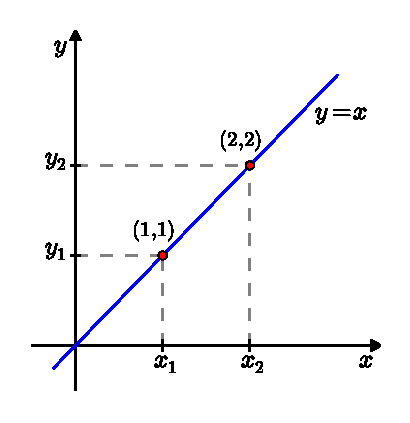
\includegraphics[scale=0.9]{./cap_interp/pics/ex_intro_interpolacao/ex_intro_interpolacao}
  \caption{Exemplo de interpolação de dois pontos por uma reta, veja o Exemplo~\ref{ex:intro_interpolacao}.}\label{fig:ex_intro_interp}
\end{figure}

\begin{ex}\label{ex:intro_interpolacao}
  Um dos problemas de interpolação mais simples é o de encontrar a equação da reta que passa por dois pontos dados. Por exemplo, sejam dados o conjunto de pontos $\{(1, 1), (2, 2)\}$ e a família de funções $\mathcal{F}_{[1,2]}$:
  \begin{equation}
   \mathcal{F}_{[1,2]} = \left\{f:[1,2]\rightarrow \mathbb{R}~;~[1,2]\ni x\mapsto f(x) = a + bx;\,a,b\in\mathbb{R}\right\}.
  \end{equation}
  Para que uma $f$ na família seja a função interpoladora do conjunto de pontos dados, precisamos que
  \begin{equation}
    \begin{array}{l}
      a + bx_1 = y_1\\
      a + bx_2 = y_2
    \end{array}\quad\text{isto é}\quad
    \begin{array}{l}
      a + b = 1\\
      a + 2b = 2
    \end{array}
  \end{equation}
o que nos fornece $a = 0$ e $b = 1$. Então, a função interpoladora $f$ é tal que  $f(x) = x$ para um $x\in[1,2]$. Os pontos e a reta interpolada estão esboçados na Figura~\ref{fig:ex_intro_interp}.
\end{ex}

Um problema de interpolação cuja família de funções constitui-se de polinômios é chamado de problema de interpolação polinomial.

%%%%%%%%%%%%%%%%%%%%
% python
%%%%%%%%%%%%%%%%%%%%
\ifispython
Ao longo do capítulo, faremos alguns comentários usando códigos em \verb+Python+. Nestes, assumiremos que os seguintes módulos estão carregados:
\begin{verbatim}
import numpy as np
from numpy import linalg
from numpy.polynomial import polynomial as poly
import matplotlib.pyplot as plt
\end{verbatim}
\fi
%%%%%%%%%%%%%%%%%%%%


\section{Interpolação polinomial}\index{interpolação!polinomial}

Interpolação polinomial é um caso particular do problema geral de interpolação, no qual a família de funções é constituída de polinômios. A escolha de polinômios como funções interpolantes é natural por diversos  motivos, entre eles: se $p$ é um polinômio de grau $n$, o valor $p(x)$ para um $x$ real é calculado através de $n+1$ operações de multiplicação e $n+1$ operações de adição. Para tanto, pode-se usar o algoritmo de Horner\footnote{William George Horner, 1786 - 1837, matemático britânico.}. Dado um polinômio $p$ de grau $n$ da forma
\begin{equation}
  p(x)=\sum_{k=0}^{n}a_k x^k,
\end{equation}
é possível reescrevê-lo como a sequência de operações dada por
\begin{equation}
  a_0 + x\left(a_1 + x\left(a_2 + x\left(\ldots + x\left(a_{n-1} + x a_n\right)\ldots\right)\right)\right).
\end{equation}

Também, derivadas e primitivas de polinômios são também polinômios cuja relação algébrica com o original é simples. Além disso, o teorema da aproximação de Weierstrass estabelece que qualquer função contínua definida em um intervalo fechado pode ser aproximada uniformemente por um polinômio tão bem quanto se queira.

\begin{teo}[Weierstrass]Seja $f$ uma função contínua definida no intervalo fechado $[a,b]$ e seja $\delta$ um número positivo. Então existe um polinômio $p$, tal que para todo $x\in[a,b]$,
  \begin{equation}
    |f(x)-p(x)|<\delta.
  \end{equation}
\end{teo}

Observe que para o problema ser bem determinado, é necessário restringirmos o grau dos polinômios. Dado um conjunto de $n$ pontos a serem interpolados $\{(x_i,y_i)\}_{i=1}^{n}$, $x_i\neq x_j$ para $i\neq j$, a família de polinômios $\mathcal{F} = \mathbb{P}_{n-1}$ deve ser escolhida, onde:
\begin{equation}
  \mathbb{P}_{n-1} := \left\{p : x\mapsto p(x) = \sum_{k=0}^{n-1}a_kx^k ;\, \{a_0,a_1,\ldots,a_{n-1}\}\in\mathbb{R}\right\},
\end{equation}
isto é, a família dos polinômios reais de grau menor ou igual a $n-1$.

O Exemplo~\ref{ex:intro_interpolacao} discute um dos casos mais simples de interpolação polinomial, o qual consiste em interpolar uma reta por dois pontos. Neste caso, a família de funções consiste de polinômios de grau 1. Se buscarmos interpolar uma parábola pelos dois pontos dados, o problema fica subdeterminado, pois existem infinitas parábolas que passam por dois pontos dados. Além disso, se buscarmos interpolar uma reta por três pontos dados, o problema estaria sobredeterminado e poderia não ter solução se os pontos não fossem colineares. Veja o Exercício~\ref{exeresol:problemas_mal_determinados}.

Assim, dado um conjunto com $n$ pontos $\{(x_i,y_i)\}_{i=1}^{n}$, chamamos de \emph{polinômio interpolador}\index{polinômio interpolador} o polinômio de grau menor ou igual a $n-1$ que os interpola.


\begin{figure}[ht]
  \centering
  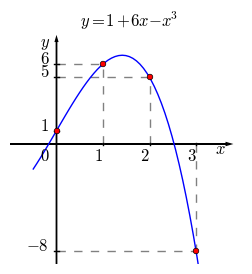
\includegraphics{./cap_interp/pics/ex_interpolacao_polinomial/ex_interpolacao_polinomial}
  \caption{Polinômio interpolador do conjunto de pontos $\{(0, 1)$, $(1, 6)$, $(2, 5)$, $(3, -8)\}$. Veja o Exemplo~\ref{ex:interpolacao_polinomial}.}\label{fig:ex_interpolacao_polinomial}
\end{figure}

\begin{ex}\label{ex:interpolacao_polinomial} Encontre o polinômio interpolador do conjunto de pontos $\{(0, 1)$, $(1, 6)$, $(2, 5)$, $(3, -8)\}$.
\end{ex}
\begin{sol}
Como o conjunto consiste de 4 pontos, o polinômio interpolador deve ser da forma:
\begin{equation}
  p(x) = a_0 + a_1x + a_2x^2 + a_3x^3.
\end{equation}
As condições de interpolação são $p(x_i) = y_i$, $i = 0, 1, 2, 3$, o que nos leva ao sistema linear:
\begin{equation}
  \begin{array}{lclclclcl}
    a_0& & & & & & &=&1\\
    a_0&+& a_1&+& a_2&+&  a_3&=&6\\
    a_0&+&2a_1&+&4a_2&+& 8a_3&=&5\\
    a_0&+&3a_1&+&9a_2&+&27a_3&=&-8
  \end{array}
\end{equation}
cuja solução é $a_0=1$, $a_1=6$, $a_2=0$ e $a_3=-1$. Portanto, o polinômio interpolador é $p(x)=1+6x-x^3$. Veja Figura~\ref{fig:ex_interpolacao_polinomial}.

%%%%%%%%%%%%%%%%%%%%
% scilab
%%%%%%%%%%%%%%%%%%%%
\ifisscilab
No \verb+Scilab+, podemos encontrar o polinômio interpolador e esboçar seu gráfico com os seguintes comandos:
\begin{verbatim}
-->xi = [0 1 2 3]';
-->yi = [1 6 5 -8]';
-->A = [xi.^0 xi.^1 xi.^2 xi.^3];
-->a = A\yi;
-->p = poly(a,'x','c')
  p  =
               3
     1 + 6x - x
-->xx = linspace(-0.5,3.25);
-->plot(xi,yi,'ro',xx,horner(p,xx),'b-');xgrid
\end{verbatim}
\fi
%%%%%%%%%%%%%%%%%%%%
%%%%%%%%%%%%%%%%%%%%
% octave
%%%%%%%%%%%%%%%%%%%%
\ifisoctave
No \verb+GNU Octave+, podemos encontrar o polinômio interpolador e esboçar seu gráfico com os seguintes comandos:
\begin{verbatim}
xi = [0 1 2 3]';
yi = [1 6 5 -8]';
A = [xi.^3 xi.^2 xi.^1 xi.^0];
a = A\yi;
xx = linspace(-0.5,3.25);
plot(xi,yi,'ro',xx,polyval(a,xx),'b-');xgrid
\end{verbatim}
\fi
%%%%%%%%%%%%%%%%%%%%
%%%%%%%%%%%%%%%%%%%%
% python
%%%%%%%%%%%%%%%%%%%%
\ifispython
Em \verb+Python+, podemos encontrar o polinômio interpolador e esboçar seu gráfico com os seguintes comandos:
\begin{verbatim}
>>> xi = np.array([0,1,2,3], dtype='double')
>>> yi = np.array([1,6,5,-8], dtype='double')
>>> A = np.array([xi**3,xi**2,xi**1,xi**0]).transpose()
>>> a = np.linalg.inv(A).dot(yi);a
array([ -1,  0.,  6,  1. ])
>>> xx = np.linspace(-0.5,3.25);
>>> plt.plot(xi,yi,'ro',xx,np.polyval(a,xx),'b-')
>>> plt.grid();plt.show()
\end{verbatim}
\fi
%%%%%%%%%%%%%%%%%%%%
\end{sol}


\begin{teo}\label{teo:interp_poli} Seja $\{(x_i,y_i)\}_{i=1}^{n}$ um conjunto de $n$ pares ordenados de números reais tais que $x_i \ne x_j$ se $i\ne j$, então existe um único polinômio $p(x)$ de grau $n-1$ ou inferior que passa por todos os pontos dados, isto é, $p(x_i)=y_i, i=1,\ldots, n$.
\end{teo}
\begin{proof} Observe que o problema de encontrar os coeficientes $a_0$, $a_1$,\ldots, $a_{n-1}$ do polinômio
\begin{equation} p(x)=a_0+a_1x+a_2x^2+\cdots a_{n-1}x^{n-1}=\sum_{k=0}^{n-1} a_k x^k \end{equation}
tal que $p(x_i)=y_i$ é equivalente a resolver o sistema linear com $n$ equações e $n$ incógnitas dado por
\begin{equation}
  \begin{split}
    a_0+a_1x_1+a_1x_1^2+\cdots +a_{n-1} x_1^{n-1} &= y_1,\\
    a_0+a_1x_2+a_2x_2^2+\cdots +a_{n-1} x_2^{n-1} &= y_2,\\
    &\vdots\\
    a_0+a_1x_n+a_2x_n^2+\cdots +a_{n-1} x_n^{n-1}&= y_n.
  \end{split}
\end{equation}
O qual pode ser escrito na forma matricial como
\begin{equation}
  \begin{bmatrix}
    1 & x_1 & x_1^2 & \cdots & x_1^{n-1}\\
    1 & x_2 & x_2^2 & \cdots & x_2^{n-1}\\
    1 & x_3 & x_3^2 & \cdots & x_3^{n-1}\\
    \vdots&\vdots&\vdots&\ddots&\vdots\\
    1 & x_n & x_n^2 & \cdots & x_n^{n-1}
  \end{bmatrix}
  \begin{bmatrix}
    a_0\\a_1\\a_2\\ \vdots \\a_{n-1}
  \end{bmatrix} =
  \begin{bmatrix}
    y_1\\y_2\\y_3\\ \vdots \\y_n
  \end{bmatrix}
\end{equation}
A matriz envolvida é uma \emph{matriz de Vandermonde}\footnote{Alexandre-Théophile Vandermonde, 1735 - 1796, matemático francês.}\index{matriz de Vandermonde} de ordem $n$ cujo determinante é dado pelo produtório duplo
\begin{equation} \prod_{1\leq i<j\leq n}\left(x_j-x_i\right) \end{equation}
É fácil ver que se as abscissas são diferentes dois a dois, então o determinante é não nulo. Disto decorre que a matriz envolvida é inversível e, portanto, o sistema possui uma solução que é única.
\end{proof}

% \begin{ex} Encontre o polinômio da forma $P(x)=a_0+a_1x+a_2x^2+a_3x^3$ que passa pelos pontos
% \begin{equation} (0,0),(1,1),(2,4),(3,9) \end{equation}
% Este problema é equivalente ao seguinte sistema linear:
% \begin{eqnarray}
% a_0&=&0\\
% a_0+a_1+a_2+a_3&=&1\\
% a_0+2a_1+4a_2+8a_3&=&4\\
% a_0+3a_1+9a_2+27a_3&=&9
% \end{eqnarray}
% cuja solução é $a_0=0$, $a_1=0$, $a_2=1$ e $a_3=0$. Portanto
% \begin{equation} P(x)=x^2 \end{equation}
% \end{ex}

Esta abordagem direta que usamos no Exemplo~\ref{ex:interpolacao_polinomial} e na demonstração do Teorema~\ref{teo:interp_poli} se mostra ineficiente quando o número de pontos é grande e quando existe grande variação nas abscissas. Neste caso, a matriz de Vandermonde é mal condicionada (ver \cite{Gautschi}), o que acarreta um aumento dos erros de arredondamento na solução do sistema.

Uma maneira de resolver este problema é escrever o polinômio em uma base que produza um sistema bem condicionado.

\subsection*{Exercícios resolvidos}

\construirExeresol

\begin{exeresol}\label{exeresol:problemas_mal_determinados}
  Mostre que:
  \begin{itemize}
  \item[a)] Existem infinitas parábolas que interpolam dois pontos dados $\{(x_1, y_1), (x_2, y_2)\}$, com $x_1 \neq x_2$.
  \item[b)] Não existe reta que interpola os pontos $\{(1, 1), (2, 2,1), (3, 3)\}$.
  \item[c)] Não existe parábola de equação $y = a_0 + a_1x + a_2x^2$ que interpola dois pontos dados $\{(x_1, y_1), (x_1, y_2)\}$, com $y_1 \neq y_2$. Mas, existem infinitas parábolas de equação $x = a_0 + a_1y + a_2y^2$ que interpolam estes pontos.
  \end{itemize}
\end{exeresol}
\begin{resol}
  \begin{itemize}
  \item[a)] Uma parábola de equação $y = a_1 + a_2x + a_3x^2$ que interpola os pontos deve satisfazer o sistema:
    \begin{equation}
      \begin{split}
        a_1 + a_2x_1 + a_3x_1^2 &= y_1\\
        a_1 + a_2x_2 + a_3x_2^2 &= y_2
      \end{split}
    \end{equation}
    Sem perda de generalidade, para cada $a_3\in\mathbb{R}$ dado, temos:
    \begin{equation}
      \begin{split}
        a_1 + a_2x_1  &= y_1 - a_3x_1^2\\
        a_1 + a_2x_2  &= y_2 - a_3x_2^2
      \end{split},
    \end{equation}
    o qual tem solução única, pois $x_1\neq x_2$. Ou seja, para cada $a_3\in\mathbb{R}$ dado, existem $a_1, a_2\in\mathbb{R}$ tais que a parábola de equação $y = a_1 + a_2x + a_3x^2$ interpola os pontos dados.
  \item[b)] Certamente não existem retas de equação $x = a$ que interpolam os pontos dados. Consideremos então retas de equação $y = a_1 + a_2x$. Para uma tal reta interpolar os pontos dados é necessário que:
    \begin{equation}
      \begin{split}
        a_1 + a_2 = 1\\
        a_1 + 2a_2 = 2,1\\
        a_1 + 3a_2 = 3
      \end{split},
    \end{equation}
    o qual é um sistema impossível.
  \item[c)] Não existe uma parábola de equação $y = a_1 + a_2x + a_3x^2$ que interpole os pontos dados, pois tal equação determina uma função de $x$ em $y$. Agora, para mostrar que existem infinitas parábolas de equação $x = a_1 + a_2y + a_3y^2$ que interpolam os pontos dados, basta seguir um raciocínio análogo ao do item a), trocando $x$ por $y$ e $y$ por $x$.
  \end{itemize}
\end{resol}

\subsection*{Exercícios}

\construirExer

\begin{exer}\label{exer:interp1}
Encontre o polinômio interpolador para o conjunto de pontos $\{(-2, -47)$, $(0, -3)$, $(1, 4)$, $(2, 41)\}$. Então, faça um gráfico com os pontos e o polinômio interpolador encontrado.
\end{exer}
\begin{resp}
  $p(x) = -3 + 2x + 5x^3$.
\end{resp}

\begin{exer}
  Encontre o polinômio interpolador para o conjunto de pontos $\{(-1, 1,25)$, $(0,5, 0,5)$, $(1, 1,25)$, $(1,25, 1,8125)\}$.
\end{exer}
\begin{resp}
  $p(x) = 0,25 + x^2$.
\end{resp}

\section{Diferenças divididas de Newton}\index{diferenças divididas de Newton}
Dado um conjunto com $n$ pontos $\{(x_i, y_i)\}_{i=1}^n$, o \emph{método das diferenças divididas de Newton} consiste em construir o polinômio interpolador da forma
\begin{equation}
  \begin{split}
    p(x) &= a_1 + a_2 (x-x_1) + a_3 (x-x_1)(x-x_2) + \cdots \\
         &+ a_n (x-x_1)(x-x_2)\cdots (x-x_{n-1}).
  \end{split}
\end{equation}
Como $p(x_i) = y_i$, $i=1, 2, \dotsc, n$, os coeficientes $a_i$ satisfazem o seguinte sistema triangular inferior:
\begin{small}
  \begin{equation}
    \begin{array}{ll}
a_1               &= y_1\\
a_1+a_2(x_2-x_1)  &= y_2\\
a_1+a_2(x_3-x_1)+a_3(x_3-x_1)(x_3-x_2) &= y_3\\
&\vdots\\
a_1+a_2(x_n-x_1)+\cdots + a_n(x_n-x_1)\cdots (x_n-x_{n-1}) &= y_n
    \end{array}
  \end{equation}
\end{small}
Resolvendo de cima para baixo, obtemos
\begin{equation}\label{eq:coef_dif_div}
  \begin{split}
a_1&=y_1\\
a_2&=\frac{y_2-a_1}{x_2-x_1}=\frac{y_2-y_1}{x_2-x_1}\\
a_3&=\frac{y_3-a_2(x_3-x_1)-a_1}{(x_3-x_1)(x_3-x_2)}=\frac{\frac{y_3-y_2}{(x_3-x_2)}-\frac{y_2-y_1}{(x_2-x_1)}}{(x_3-x_1)}\\
&\ldots
  \end{split}
\end{equation}

Note que os coeficientes são obtidos por diferenças das ordenadas divididas por diferenças das abscissas dos pontos dados. Para vermos isso mais claramente, introduzimos a seguinte notação:
\begin{eqnarray}
  f[x_j]&:=&y_j\\
  f[x_j, x_{j+1}]&:=&\frac{f[x_{j+1}]-f[x_j]}{x_{j+1}-x_j}\\
  f[x_j, x_{j+1}, x_{j+2}]&:=&\frac{f[x_{j+1}, x_{j+2}]-f[x_j, x_{j+1}]}{x_{j+2}-x_j}\\
        &\vdots&\\
  f[x_j, x_{j+1}, \dotsc, x_{j+k}] &:=& \frac{f[x_{j+1}, x_{j+2}, \dotsc, x_{j+k}]-f[x_j, x_{j+1}, \dotsc, x_{j+k-1}]}{x_{j+k}-x_j}
\end{eqnarray}
Chamamos $f[x_j]$ de diferença dividida de ordem zero (ou primeira diferença dividida), $f[x_i,x_j+1]$ de diferença dividida de ordem 1 (ou segunda diferença dividida) e assim por diante.

Uma inspeção cuidadosa dos coeficientes obtidos em \eqref{eq:coef_dif_div} nos mostra que
\begin{equation}
 a_k=f[x_1,x_2,\ldots,x_k]
\end{equation}
Isto nos permite esquematizar o método conforme apresentado na Tabela~\ref{tab:esquema_difdiv}.

\begin{table}
  \centering
  \caption{Esquema de diferenças divididas para um conjunto com três pontos $\{(x_i, y_i)\}_{i=1}^3$.}
  \label{tab:esquema_difdiv}
\begin{tabular}{c||c|ccc}\hline
$j$ & $x_j$ & $f[x_j]$ & $f[x_{j-1},x_j]$ & $f[x_{j-2},x_{j-1},x_j]$ \\\hline
$1$ & $x_1$ & $\pmb{f[x_1]}=y_1$ & &\\
&&&$\displaystyle \pmb{f[x_1,x_2]}=\frac{f[x_2]-f[x_1]}{x_2-x_1}$&\\
$2$ & $x_2$ & $f[x_2] = y_2$ && $\displaystyle \pmb{f[x_1,x_2,x_3]}=\frac{f[x_2,x_3]-f[x_1,x_2]}{x_3-x_1}$\\
&&&$\displaystyle f[x_2,x_3]=\frac{f[x_3]-f[x_2]}{x_3-x_2}$ &\\
$3$ & $x_3$ & $f[x_3]=y_3$ &&\\\hline
\end{tabular}
\end{table}

\begin{ex}
Use o método de diferenças divididas para encontrar o polinômio que passe pelos pontos $(-1,3),(0,1),(1,3),(3,43)$.
\end{ex}
\begin{sol}
Usando o esquema apresentado na Tabela~\ref{tab:esquema_difdiv}, obtemos
\begin{center}
\begin{tabular}{c||c|cccc}\hline
 $j$ & $x_j$ & $f[x_j]$ & $f[x_{j-1},x_j]$ & $f[x_{j-2},x_{j-1},x_j]$ & $f[x_{j-3},x_{j-2},x_{j-1},x_j]$\\\hline
$1$ & $-1$ & $\pmb{3}$&&&\\
&&&$\displaystyle \frac{1-3}{0-(-1)}=\pmb{-2}$&&\\
$2$&$0$&$1$&&$\displaystyle \frac{2-(-2)}{1-(-1)}=\pmb{2}$&\\
&&&$\displaystyle \frac{3-1}{1-0}=2$&&$\displaystyle\frac{6-2}{3-(-1)}=\pmb{1}$\\
$3$&$1$&$3$&&$\displaystyle \frac{20-2}{3-0}=6$&\\
&&&$\displaystyle \frac{43-3}{3-1}=20$&&\\
$4$&$3$&$43$&&&\\\hline
\end{tabular}
\end{center}
Portanto, o polinômio interpolador do conjunto de pontos dados é
\begin{equation}
  p(x) = 3-2(x+1)+2(x+1)x+(x+1)x(x-1)
\end{equation}
ou, equivalentemente, $p(x) = x^3+2x^2-x+1$.

%%%%%%%%%%%%%%%%%%%%
% octave
%%%%%%%%%%%%%%%%%%%%
\ifisoctave
No \verb+GNU Octave+, podemos fazer as contas acima da segunte forma:
\begin{verbatim}
x = [-1,0,1,3]';
y = [3,1,3,43]';
#inicializando a tabela
T = zeros(4,4);
#primeira coluna
T(:,1)=y;
#segunda coluna
T(2,2)=(T(2,1)-T(1,1))/(x(2)-x(1));
T(3,2)=(T(3,1)-T(2,1))/(x(3)-x(2));
T(4,2)=(T(4,1)-T(3,1))/(x(4)-x(3));
#terceira coluna
T(3,3)=(T(3,2)-T(2,2))/(x(3)-x(1));
T(4,3)=(T(4,2)-T(3,2))/(x(4)-x(2));
#quarta coluna
T(4,4)=(T(4,3)-T(3,3))/(x(4)-x(1));
#polinomio interpolador
p = T(1,1);
p = [0, p] + T(2,2)*[1,-x(1)];
p = [0, p] + T(3,3)*conv([1,-x(1)],[1,-x(2)]);
p = [0, p] + T(4,4)*conv(conv([1,-x(1)],[1,-x(2)]),[1,-x(3)]);
\end{verbatim}
\fi
%%%%%%%%%%%%%%%%%%%%
%%%%%%%%%%%%%%%%%%%%
% python
%%%%%%%%%%%%%%%%%%%%
\ifispython
Em \verb+Python+, podemos fazer as contas acima da segunte forma:
\begin{verbatim}
x = np.array([-1,0,1,3], dtype="double")
y = np.array([3,1,3,43], dtype="double")
#inicializando a tabela
T = np.zeros((4,4));
#primeira coluna
T[:,0]=y;
#segunda coluna
T[1,1]=(T[1,0]-T[0,0])/(x[1]-x[0]);
T[2,1]=(T[2,0]-T[1,0])/(x[2]-x[1]);
T[3,1]=(T[3,0]-T[2,0])/(x[3]-x[2]);
#terceira coluna
T[2,2]=(T[2,1]-T[1,1])/(x[2]-x[0]);
T[3,2]=(T[3,1]-T[2,1])/(x[3]-x[1]);
#quarta coluna
T[3,3]=(T[3,2]-T[2,2])/(x[3]-x[0]);
print(T)
#polinomio interpolador
p = np.array([T[0,0]], dtype="double")
paux = np.array([-x[0],1], dtype="double")
p.resize(2)
p += T[1,1]*paux
paux = poly.polymul(paux,[-x[1],1])
p.resize(3)
p += T[2,2]*paux
paux = poly.polymul(paux,[-x[2],1])
p.resize(4)
p += T[3,3]*paux
\end{verbatim}
\fi
%%%%%%%%%%%%%%%%%%%%
\end{sol}

\section{Polinômios de Lagrange}\index{polinômios!de Lagrange}
Outra maneira clássica de resolver o problema da interpolação polinomial é através dos polinômios de Lagrange. Dado um conjunto de pontos $\{x_j\}_{j=1}^n$ distintos dois a dois, definimos os polinômios de Lagrange como os polinômios de grau $n-1$ que satisfazem
\begin{equation}
L_k(x_j)=\left\{\begin{array}{rl}
1,& \text{se }k=j\\
0,& \text{se }k\neq j
\end{array}
\right.
\end{equation}
Assim, o polinômio $p(x)$ de grau $n-1$ que interpola os pontos dados, isto é, $p(x_j)=y_j, j=1,\ldots,n$ é dado por
\begin{equation}
  p(x)=y_1L_1(x)+y_2L_2(x)+\cdots +y_nL_n(x)=\sum_{k=1}^n y_k L_k(x).
\end{equation}

Para construir os polinômios de Lagrange, podemos analisar a sua forma fatorada, ou seja:
\begin{equation} L_k(x)=c_k\prod_{\substack{j=1\\j\ne k}}^{n} (x-x_j) \end{equation}
onde o coeficiente $c_k$ é obtido da condição $L_k(x_k)=1$:
\begin{equation} L_k(x_k)=c_k\prod_{\substack{j=1\\j\ne k}}^{n} (x_k-x_j) \Longrightarrow  c_k=\frac{1}{\displaystyle \prod_{\substack{j=1\\j\ne k}}^{n} (x_k-x_j)} \end{equation}
Portanto,
\begin{equation} L_k(x)=\prod_{\substack{j=1\\j\ne k}}^{n} \frac{(x-x_j)}{(x_k-x_j)} \end{equation}

\begin{obs} O problema de interpolação quando escrito usando como base os polinômios de Lagrange produz um sistema linear diagonal.
\end{obs}

\begin{ex}
  Encontre o polinômio da forma $p(x)=a_1+a_2x+a_3x^2+a_4x^3$ que passa pelos pontos $(0, 0)$, $(1, 1)$, $(2, 4)$, $(3, 9)$.
\end{ex}
\begin{sol}
Escrevemos:
\begin{eqnarray}
  L_1(x)&=& \frac{(x-1)(x-2)(x-3)}{(0-1)(0-2)(0-3)}=-\frac{1}{6}x^3+x^2-\frac{11}{6}x+1\\
  L_2(x)&=& \frac{x(x-2)(x-3)}{1(1-2)(1-3)}=\frac{1}{2}x^3-\frac{5}{2}x^2+3x\\
  L_3(x)&=& \frac{x(x-1)(x-3)}{2(2-1)(2-3)}=-\frac{1}{2}x^3+2x^2-\frac{3}{2}x\\
  L_4(x)&=& \frac{x(x-1)(x-2)}{3(3-1)(3-2)}=\frac{1}{6}x^3-\frac{1}{2}x^2+\frac{1}{3}x
\end{eqnarray}
Assim, temos:
\begin{equation}
  P(x)=0\cdot L_1(x)+1\cdot L_2(x)+4\cdot L_3(x)+9\cdot L_4(x)=x^2
\end{equation}

%%%%%%%%%%%%%%%%%%%%
% octave
%%%%%%%%%%%%%%%%%%%%
\ifisoctave
No \verb+GNU Octave+, podemos fazer as contas acima da segunte forma:
\begin{verbatim}
x = [0 1 2 3]';
y = [0 1 4 9]';
#L1
num = poly([x(2),x(3),x(4)]);
L1 = num/polyval(num,x(1));
#L2
num = poly([x(1),x(3),x(4)]);
L2 = num/polyval(num,x(2));
#L3
num = poly([x(1),x(2),x(4)]);
L3 = num/polyval(num,x(3));
#L4
num = poly([x(1),x(2),x(3)]);
L4 = num/polyval(num,x(4));
p = y(1)*L1 + y(2)*L2 + y(3)*L3 + y(4)*L4
\end{verbatim}
\fi
%%%%%%%%%%%%%%%%%%%%
\end{sol}

\section{Aproximação de funções reais por polinômios interpoladores}\index{aproximação!de funções!por polinômios}

\begin{teo}\label{teo_interp}
Dados $n+1$ pontos distintos, $x_0,\ x_1,\ \cdots,\ x_n$, dentro de um intervalo $[a,b]$ e uma função $f$ com $n+1$ derivadas contínuas nesse intervalo ($f\in C^{n+1}[a,b]$), então para cada $x$ em $[a,b]$, existe um número $\xi(x)$ em $(a,b)$ tal que
\begin{equation}
f(x)=P(x)+\frac{f^{(n+1)}(\xi(x))}{(n+1)!}(x-x_0)(x-x_1)\cdots(x-x_n),
\end{equation}
onde $P(x)$ é o polinômio interpolador. Em especial, pode-se dizer que
\begin{equation}
|f(x)-P(x)|\leq \frac{M}{(n+1)!}\left|(x-x_0)(x-x_1)\cdots(x-x_n)\right|,
\end{equation}
onde
\begin{equation}
M=\max_{x\in[a,b]}|f^{(n+1)}(\xi(x))|
\end{equation}
\end{teo}

\begin{ex}
Considere a função $f(x)=\cos(x)$ e o polinômio $P(x)$ de grau 2 tal que $P(0)=\cos(0)=1$, $P(\frac{1}{2})=\cos(\frac{1}{2})$ e $P(1)=\cos(1)$. Use a fórmula de Lagrange para encontrar $P(x)$. Encontre o erro máximo que se assume ao aproximar o valor de $\cos(x)$ pelo de $P(x)$ no intervalo $[0,1]$. Trace os gráficos de $f(x)$ e $P(x)$ no intervalo $[0,1]$ no mesmo plano cartesiano e, depois, trace o gráfico da diferença $\cos(x)-P(x)$. Encontre o erro efetivo máximo $|\cos(x)-P(x)|$.
\end{ex}
\begin{sol}
  Usando polinômios de Lagrange, obtemos
  \begin{eqnarray}
    P(x) &=& 1\frac{(x-\frac{1}{2})(x-1)}{(0-\frac{1}{2})(0-1)}\nonumber\\
         &+& \cos\left(\frac{1}{2}\right)\frac{(x-0)(x-1)}{(\frac{1}{2}-0)(\frac{1}{2}-1)}\nonumber\\
         &+& \cos(1)\frac{(x-0)(x-\frac{1}{2})}{(1-0)(1-\frac{1}{2})}\\
         &\approx&   1 - 0,0299720583066x - 0,4297256358252x^2
  \end{eqnarray}

%%%%%%%%%%%%%%%%%%%%
% scilab
%%%%%%%%%%%%%%%%%%%%
\ifisscilab
No \verb+Scilab+, podemos computar o polinômio interpolador da seguinte forma:
\begin{verbatim}
L1=poly([.5 1],'x');L1=L1/horner(L1,0)
L2=poly([0 1],'x');L2=L2/horner(L2,0.5)
L3=poly([0 .5],'x');L3=L3/horner(L3,1)
P=L1+cos(.5)*L2+cos(1)*L3
x=[0:.05:1]
plot(x,cos)
plot(x,horner(P,x),'red')
plot(x,horner(P,x)-cos(x))
\end{verbatim}
\fi
%%%%%%%%%%%%%%%%%%%%
%%%%%%%%%%%%%%%%%%%%
% octave
%%%%%%%%%%%%%%%%%%%%
\ifisoctave
No \verb+GNU Octave+, podemos computar o polinômio interpolador da seguinte forma:
\begin{verbatim}
L1=poly([.5 1]);L1=L1/polyval(L1,0)
L2=poly([0 1]);L2=L2/polyval(L2,0.5)
L3=poly([0 .5]);L3=L3/polyval(L3,1)
P=L1+cos(.5)*L2+cos(1)*L3
\end{verbatim}
\fi
%%%%%%%%%%%%%%%%%%%%
%%%%%%%%%%%%%%%%%%%%
% python
%%%%%%%%%%%%%%%%%%%%
\ifispython
\construirPython
\fi
%%%%%%%%%%%%%%%%%%%%

Para estimar o erro máximo, precisamos estimar a derivada terceira de $f(x)$:
\begin{equation} |f'''(x)|=|\sin(x)|\leq \sin(1)<0,85 \end{equation}
e, assim,
\begin{equation}
\max_{x\in[0,1]} \left|x\left(x-\frac{1}{2}\right)(x-1)\right|.
\end{equation}
O polinômio de grau três $Q(x)=x\left(x-\frac{1}{2}\right)(x-1)$ tem um mínimo (negativo) em $x_1=\frac{3+\sqrt{3}}{6}$ e um máximo (positivo) em $x_2=\frac{3-\sqrt{3}}{6}$. Logo:
\begin{equation}
\max_{x\in[0,1]} \left|x\left(x-\frac{1}{2}\right)(x-1)\right|\leq \max\{|Q(x_1)|,\ |Q(x_2)|\}\approx 0,0481125.
\end{equation}
Portanto:
\begin{equation}
|f(x)-P(x)|< \frac{0,85}{3!}0,0481125\approx 0,0068159<7\cdot 10^{-3}
\end{equation}

Para estimar o erro efetivo máximo, basta encontrar o máximo de $|P(x)-\cos(x)|$. O mínimo (negativo) de $P(x)-\cos(x)$ acontece em $x_1=4,29\cdot 10^{-3}$ e o máximo (positivo) acontece em $x_2=3,29\cdot 10^{-3}$. Portanto, o erro máximo efetivo é $4,29\cdot 10^{-3}$.
\end{sol}


\begin{ex}\label{exemp_simpson}
Considere o problema de aproximar o valor da integral $\int_0^1 f(x)dx$ pelo valor da integral do polinômio $P(x)$ que coincide com $f(x)$ nos pontos $x_0=0$, $x_1=\frac{1}{2}$ e $x_2=1$. Use a fórmula de Lagrange para encontrar $P(x)$. Obtenha o valor de $\int_0^1P(x)dx$ e encontre uma expressão para o erro de truncamento.
\end{ex}
O polinômio interpolador de $f(x)$ é
\begin{eqnarray}
P(x)&=&f(0)\frac{(x-\frac{1}{2})(x-1)}{(0-\frac{1}{2})(0-1)}+f\left(\frac{1}{2}\right)\frac{(x-0)(x-1)}{(\frac{1}{2}-0)(\frac{1}{2}-1)}+f(1)\frac{(x-0)(x-\frac{1}{2})}{(1-0)(1-\frac{1}{2})}\\
&=&   f(0)(2x^2-3x+1)+f\left(\frac{1}{2}\right)(-4x^2+4x)+f(1)(2x^2-x)
\end{eqnarray}
e a integral de $P(x)$ é:
\begin{eqnarray}
\int_0^1 P(x)dx &=& \left[f(0)\left(\frac{2}{3}x^3 - \frac{3}{2}x^2+x\right)\right]_0^1 + \left[f\left(\frac{1}{2}\right)\left(-\frac{4}{3}x^3+2x^2\right)\right]_0^1 \\
&+& \left[f(1)\left(\frac{2}{3}x^3-\frac{1}{2}x^2\right)\right]_0^1\\
&=& f(0)\left(\frac{2}{3}-\frac{3}{2}+1\right)+f\left(\frac{1}{2}\right)\left(-\frac{4}{3}+2\right)+f(1)\left(\frac{2}{3}-\frac{1}{2}\right)\\
&=& \frac{1}{6}f(0)+\frac{2}{3}f\left(\frac{1}{2}\right)+\frac{1}{6}f(1)
\end{eqnarray}
Para fazer a estimativa de erro usando o Teorema~\ref{teo_interp} e temos
\begin{eqnarray}
\left|\int_0^1f(x)dx-\int_0^1 P(x)dx\right|&=&\left|\int_0^1f(x)- P(x)dx\right|\\
&\leq&\int_0^1|f(x)- P(x)|dx\\
&\leq& \frac{M}{6}  \int_0^1\left|x\left(x-\frac{1}{2}\right)(x-1)\right|dx\\
&=& \frac{M}{6}  \left[\int_0^{1/2}x\left(x-\frac{1}{2}\right)(x-1)dx\right.\\
&-&\left.\int_{1/2}^1x\left(x-\frac{1}{2}\right)(x-1)dx\right]\\
&=& \frac{M}{6}  \left[\frac{1}{64}-\left(-\frac{1}{64}\right)\right]=\frac{M}{192}.
\end{eqnarray}
Lembramos que $M=\max_{x\in[0,1]}|f'''(x)|$.

\begin{obs}Existem estimativas melhores para o erro de truncamento para este esquema de integração numérica. Veremos com mais detalhes tais esquemas na teoria de integração numérica.
\end{obs}

\begin{ex}
Use o resultado do exemplo anterior para aproximar o valor das seguintes integrais:\\

a) $\displaystyle \int_0^1 \ln(x+1) dx$\\

b) $\displaystyle \int_0^1 e^{-x^2}dx$

\end{ex}
\begin{sol}
Usando a fórmula obtida, temos que
\begin{equation}
\int_0^1\ln(x+1) dx \approx 0,39\pm \frac{1}{96}
\end{equation}
\begin{equation}
\int_0^1 e^{-x^2} dx \approx 0,75\pm \frac{3,87}{192}
\end{equation}
\end{sol}

\subsection*{Exercícios}

\begin{exer}
  Use as mesmas técnicas usadas o resultado do Exemplo~\ref{exemp_simpson} para obter uma aproximação do valor de:
  \begin{equation}
    \int_0^1 f(x)dx
  \end{equation}
através do polinômio interpolador que coincide com $f(x)$ nos pontos $x=0$ e $x=1$.
\end{exer}
\begin{resp}

  $\int_0^1 P(x)dx =\frac{f(0)+f(1)}{2}$, $\frac{1}{12}\max_{x\in[0,1]}|f''(x)|$

\end{resp}

\section{Interpolação linear segmentada}\index{interpolação!linear segmentada}
Considere o conjunto $\left(x_i,y_i\right)_{j=1}^n$ de $n$ pontos. Assumiremos que $x_{i+1}>x_i$, ou seja, as abscissas são distintas e estão em ordem crescente. A função linear que interpola os pontos $x_i$ e $x_{i+1}$ no intervalo $i$ é dada por
\begin{equation} P_i(x)=y_i \frac{(x_{i+1}-x)}{(x_{i+1}-x_i)} + y_{i+1} \frac{(x-x_i)}{(x_{i+1}-x_i)} \end{equation}

O resultado da interpolação linear segmentada é a seguinte função contínua definida por partes no intervalo $[x_1,x_n]$:
\begin{equation} f(x)=P_i(x), ~~~~ x\in [x_i,x_{i+1}] \end{equation}

\begin{ex}
  Construa uma função linear por partes que interpola os pontos $(0,0)$, $(1,4)$, $(2,3)$, $(3,0)$, $(4,2)$, $(5,0)$.

A função procurada pode ser construída da seguinte forma:
\begin{equation}
  f(x) = \left\{
    \begin{array}{ll}
      0\frac{x-1}{0-1} + 1\frac{x-0}{1-0} ,& 0 \leq x < 1\\
      4\frac{x-2}{1-2} + 3\frac{x-1}{2-1} ,& 1 \leq x < 2\\
      3\frac{x-3}{2-3} + 0\frac{x-2}{3-2} ,& 2 \leq x < 3\\
      0\frac{x-4}{3-4} + 2\frac{x-3}{4-3} ,& 3 \leq x < 4\\
      2\frac{x-5}{4-5} + 0\frac{x-4}{5-4} ,& 4 \leq x \leq 5
    \end{array}
\right.
\end{equation}
Simplificando, obtemos:
\begin{equation}
  f(x) = \left\{
    \begin{array}{ll}
        x     ,& 0 \leq x < 1\\
       -x + 5 ,& 1 \leq x < 2\\
      -3x + 9 ,& 2 \leq x < 3\\
       2x - 6 ,& 3 \leq x < 4\\
      -2x +10 ,& 4 \leq x \leq 5
    \end{array}
\right.
\end{equation}
\end{ex}

A Figura~\ref{fig:linear_segmentada} é um esboço da função $f(x)$ obtida.

%%%%%%%%%%%%%%%%%%%%
% scilab
%%%%%%%%%%%%%%%%%%%%
\ifisscilab
Ela foi gerada no \verb+Scilab+ usando os comandos:
\verbatiminput{./cap_interp/codes/interpolacao_linear_segmentada/ex_linear_segmentada.sce}
\fi
%%%%%%%%%%%%%%%%%%%%

\begin{figure}[htp]
  \begin{center}
    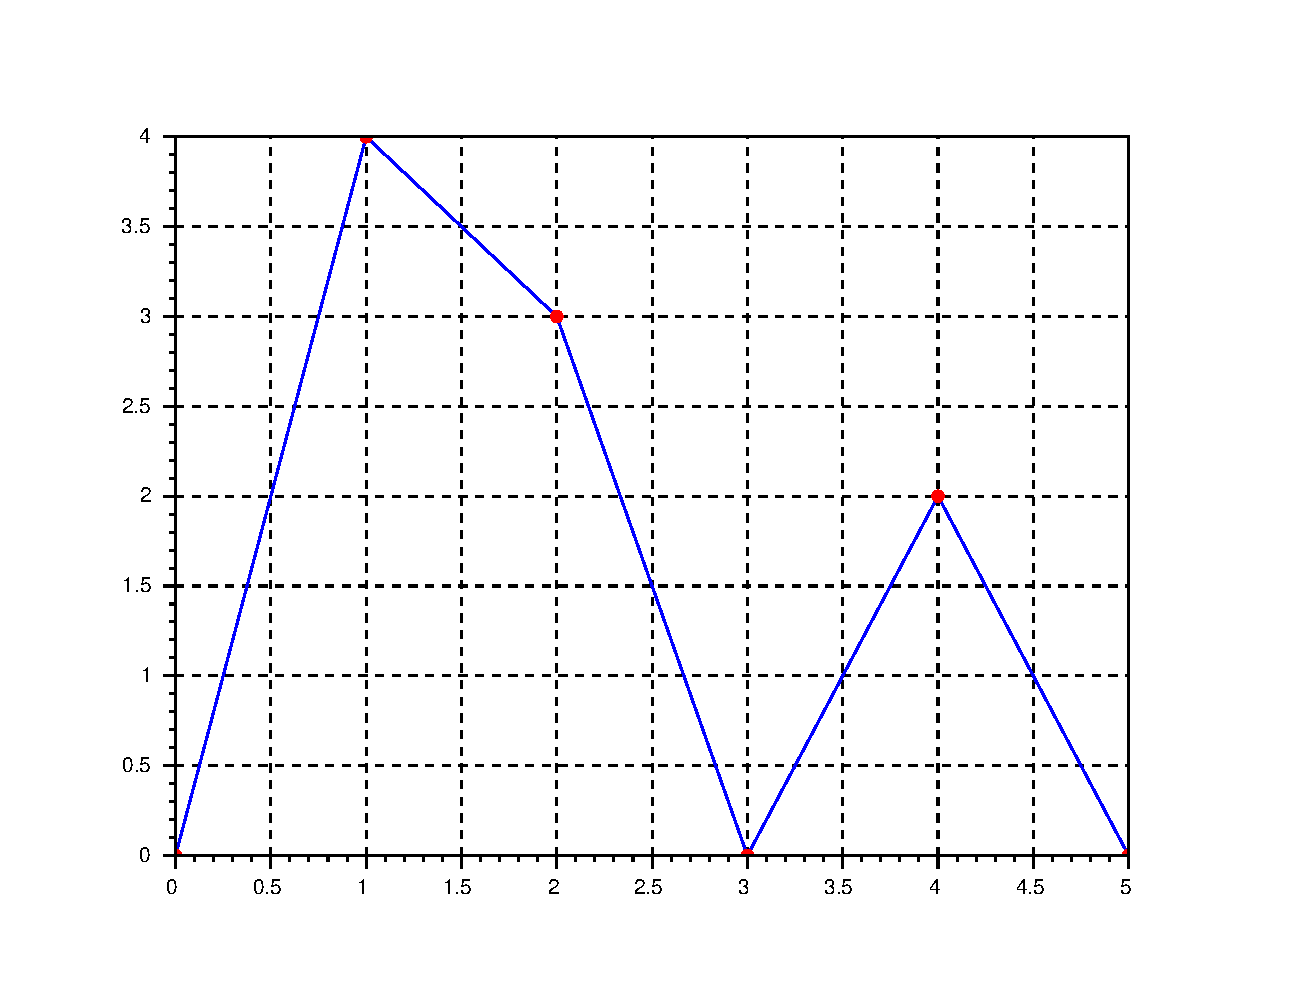
\includegraphics[scale=0.5]{./cap_interp/pics/interpolacao_linear_segmentada.eps}
    \caption{Interpolação linear segmentada.}
    \label{fig:linear_segmentada}
  \end{center}
\end{figure}


\section{Interpolação cúbica segmentada - spline}\index{interpolação!cúbica segmentada}\index{spline}
A ideia empregada na interpolação linear segmentada pode ser estendida através da utilização de polinômios de grau superior. A escolha de polinômios de grau superior implica uma maior liberdade (há um número maior de coeficientes) na construção da interpolação. Parte dessa liberdade pode ser utilizada na exigência de suavidade para a interpolação.

\begin{defn}[spline de ordem $m$]Dado um conjunto de $n$ pontos $\mathcal{I}=\left\{(x_j,y_j)\right\}_{j=1}^n$ tais que $x_{j+1}>x_j$, ou seja, as abscissas são distintas e estão em ordem crescente; um spline de ordem $m$ que interpola estes pontos é uma função $s$ com as seguintes propriedades:
\begin{itemize}
\item[i)] Em cada intervalo $[x_j,x_{j+1})$, $j=1,2,\ldots n-2$ e no segmento $[x_{n-1},x_n]$ $s$ é um polinômio de grau menor ou igual a  $m$;
\item[ii)] Em algum dos intervalos $s$ é um polinômio de grau $m$;
\item[iii)] Em cada $x_j\in \mathcal{I}$, $s(x_j)=y_j$, isto é, o spline interpola os pontos dados;
\item[iv)] $s$ é uma função de classe $\mathcal{C}^{m-1}$, isto é, é função $m-1$ vezes continuamente diferenciável.
\end{itemize}
\end{defn}

São $n-1$ intervalos e em cada um deles há $m+1$ coeficientes a se determinar. As condições \textit{iii} e \textit{iv} impostas pela definição correspondem respectivamente a $n$ e $m(n-2)$ equações. Estas últimas, se devem à exigência de continuidade nos pontos internos, ou seja, os pontos de $\mathcal{I}$ com índices $j=2,3,\ldots,n-1$. Portanto, há $m-1$ coeficientes a mais do que o número de equações e, à exceção do caso $m=1$ (interpolação linear segmentada), o problema é subdeterminado. Ou seja, uma vez fixada a ordem $m>1$, existem infinitos splines de ordem $m$ que interpolam os pontos do conjunto $\mathcal{I}$.

O caso $m=3$, denominado spline cúbico, é de grande interesse pois reproduz o comportamento físico de réguas delgadas com estrutura elástica homogênea e perfil uniforme sujeitas aos vínculos representados pelos pontos  do conjunto $\mathcal{I}$. A equação diferencial que rege o comportamento do perfil dessas réguas é um caso particular do equação da viga de Euler-Bernoulli. Neste caso, a equação tem a forma
\begin{equation}\label{eq:ed-splin3}
\dfrac{d^4y}{dx^4}=0,
\end{equation}
cuja solução geral é um polinômio de grau 3.

Vamos supor que um spline cúbico que interpola o conjunto de pontos $\mathcal{I}$ é conhecido. Como esse spline é uma função de classe $\mathcal{C}^2$, as suas derivadas nos pontos do conjunto $\mathcal{I}$  são conhecidas também. Seja $y'_j$, o valor dessa derivada em $x=x_j$. Agora, vamos considerar dois pares de pontos sucessivos de $\mathcal{I}$,  $(x_j,y_j)$ e $(x_{j+1},y_{j+1})$. A forma do spline cúbico no intervalo $[x_j,x_{j+1})$ pode ser identificada com a solução da equação diferencial \eqref{eq:ed-splin3} no intervalo $(x_j,x_{j+1})$ sujeita às condições de contorno
\begin{equation}
y(x_j)=y_j,\quad y'(x_j)=y'_j,\quad y(x_{j+1})=y_{j+1}\quad\text{e}\quad y'(x_{j+1})=y'_{j+1}.
\end{equation}
A solução desse problema de contorno é escrita de modo conveniente como
\begin{equation}
s_j(x)=a_j+b_j(x-x_j)+c_j(x-x_j)^2+d_j(x-x_j)^3,
\end{equation}
onde as constantes $a_j$, $b_j$, $c_j$ e $d_j$ se relacionam às do problema de contorno.  As duas primeiras seguem imediatamente das condições de contorno em $x_j$:
\begin{equation}
a_j=y_j\quad\text{e}\quad b_j=y'_j.
\end{equation}
As duas últimas são obtidas pela solução do sistema de equações formado pelas condições de contorno em $x_{j+1}$:
\begin{equation}
c_j=3\frac{y_{j+1}-y_j}{\left(x_{j+1}-x_j\right)^2}-\frac{y'_{j+1}+2y'_j}{x_{j+1}-x_j} \quad\text{e}\quad d_j=-2\frac{y_{j+1}-y_j}{\left(x_{j+1}-x_j\right)^3}+\frac{y'_{j+1}+y'_j}{\left(x_{j+1}-x_j\right)^2}
\end{equation}
Esta relação entre o conjunto de valores para a derivada de um spline cúbico $\{y'_j\}_{j=1}^{n}$ nos pontos de interpolação $\mathcal{I}$ e os coeficientes dos polinômios em cada intervalo de interpolação pode ser resumida na seguinte proposição:
\begin{prop}
	Seja $s$ um spline cúbico que interpola o conjunto de pontos $\mathcal{I}=\{(x_j,y_j)\}_{j=1}^n\subset\mathbb{R}^2$ tais que $x_{j+1}>x_j$. Se $\{y'_j\}_{j=1}^n$ é o conjunto dos valores da derivada de $s$ em $x_j$, então em cada intervalo $[x_j,x_{j+1})$ (fechado também à direita quando $j=n-1$) o spline é igual a $s_j$:
	\begin{equation}\label{eq:spline3}
	s_j(x)=a_j+b_j(x-x_j)+c_j(x-x_j)^2+d_j(x-x_j)^3,
	\end{equation}
	onde
	\begin{equation}
	\begin{array}{ll}\label{eq:spline3-coef}
		a_j=y_j,&c_j=3\dfrac{y_{j+1}-y_j}{h_j^2}-\dfrac{y'_{j+1}+2y'_j}{h_j},\\
		b_j=y'_j,&d_j=-2\dfrac{y_{j+1}-y_j}{h_j^3}+\dfrac{y'_{j+1}+y'_j}{h_j^2}
	\end{array}
	\end{equation}
	e
	\begin{equation}\label{eq:espacamento}
		h_j=x_{j+1}-x_j,\quad j=1,2,\ldots,n-1
	\end{equation}
	é a distância entre as abscissas de dois pontos de interpolação consecutivos.
\end{prop}
De acordo com a proposição anterior, toda informação sobre um spline cúbico é armazenada no conjunto $\{(x_j,y_j,y'_j)\}_{j=1}^n$. Por construção, uma função $s$ definida a partir de \eqref{eq:spline3}, \eqref{eq:spline3-coef} e \eqref{eq:espacamento} com um conjunto $\{(x_j,y_j,y'_j)\}_{j=1}^n\subset\mathbb{R}^3$, onde $x_{j+1}>x_j$ é de classe $\mathcal{C}^1$ mas não necessariamente um spline cúbico. Para ser um spline cúbico, os valores do conjunto $\{y'_j\}_{j=1}^n$ devem garantir a continuidade da derivada segunda de $s$ em todo intervalo $(x_1,x_n)$. Ou seja, devemos ter
\begin{equation}
\lim\limits_{x\nearrow x_{j+1} }s''_j(x)=s''_{j+1}(x_{j+1})
\end{equation}
em todos os pontos internos $j=1,2,\ldots,n-2$.  Em termos dos coeficientes dos polinômios cúbicos \eqref{eq:spline3}, a equação anterior assume a forma
\begin{equation}
2c_j+6d_jh_j=2c_{j+1},\quad j=1,2,\ldots,n-2.
\end{equation}
Esta última equação e \eqref{eq:spline3-coef} permitem construir um sistema de equações lineares para as variáveis $y'_j$:
\begin{prop} Dado o conjunto de pontos $\mathcal{I}=\{(x_j,y_j)\}_{j=1}^n\subset\mathbb{R}^2$ tais que $x_{j+1}>x_j$, as derivadas de um spline cúbico que interpola os pontos $\mathcal{I}$, $y'_j$, $j=1,2,\ldots,n$ satisfazem o sistema de equações algébricas lineares
\begin{equation}\label{eq:spline3-der}
h_jy'_{j-1}+2(h_{j-1}+h_j)y'_j+h_{j-1}y'_{j+1}=3\left(h_j\dfrac{y_j-y_{j-1}}{h_{j-1}}+h_{j-1}\dfrac{y_{j+1}-y_j}{h_j}\right),
\end{equation}
onde $j=2,3,\ldots,n-1$ e $h_j=x_{j+1}-x_j$.
\end{prop}
O sistema de equações \eqref{eq:spline3-der} é subdeterminado. São $n$ variáveis e $n-2$ equações. A inclusão de duas equações adicionais linearmente independentes das $n-2$ equações \eqref{eq:spline3-der} possibilita a existência de uma única solução. Tipicamente essas equações adicionais envolvem o comportamento do spline na fronteira ou na sua vizinhança.  A seguir, veremos quatro escolhas mais conhecidas.


\subsection{Spline natural}\index{spline!natural}

Uma forma de definir as duas equações adicionais para completar o sistema \eqref{eq:spline3-der} é impor condições de fronteira livres (ou naturais), ou seja,
\begin{equation}
s''(x_1)=s''(x_n)=0.
\end{equation}
De acordo com \eqref{eq:spline3} essas equações implicam respectivamente
\begin{equation}
c_1=0\quad\text{e}\quad 2c_{n-1}+6d_{n-1}h_{n-1}=0,
\end{equation}
ou seja,
\begin{equation}
	\left\{\begin{array}{l}
		2y'_1+y'_2=3\dfrac{y_2-y_1}{h_1}\\
		\\
		y'_{n-1}+2y'_n=3\dfrac{y_n-y_{n-1}}{h_{n-1}}
	\end{array}\right..
\end{equation}
Essas duas equações em conjunto com as equações \eqref{eq:spline3-der} formam um sistema de $n$ equações algébricas lineares $Ay'=z$, onde
\begin{equation}
	\begin{scriptsize}
		A=\left[\begin{array}{ccccccc}
			2 &1&0&0 &\cdots&0&0\\
			h_2&2(h_1+h_2)&h_1&0&\cdots&0&0\\
			0&h_3&2(h_2+h_3)&h_2&\cdots&0&0\\
			\vdots&\vdots&\vdots&\vdots&\ddots&\vdots&\vdots\\
			0&0&0&\cdots&h_{n-1} & 2(h_{n-1}+h_{n-2})&h_{n-2}\\
			0&0&0&\cdots &0&1&2
		\end{array}\right] ,
	\end{scriptsize}
\end{equation}
\begin{equation}
	y' = \left[\begin{array}{c}
		y'_1\\
		y'_2\\
		\vdots\\
		y'_n
	\end{array}\right]\qquad \text{e}\qquad
	z = 3\left[\begin{array}{c}
		\frac{y_2-y_1}{h_1}\\
		h_2\frac{y_2-y_1}{h_1}+h_1\frac{y_3-y_2}{h_2}\\
		h_3\frac{y_3-y_2}{h_2}+h_2\frac{y_4-y_3}{h_3}\\
		\vdots\\
		h_{n-1}\frac{y_{n-1}-y_{n-2}}{h_{n-2}}+h_{n-2}\frac{y_n-y_{n-1}}{h_{n-1}}\\
		\frac{y_n-y_{n-1}}{h_{n-1}}
	\end{array}\right].
\end{equation}
Observe que a matriz $A$ é diagonal dominante estrita e, portanto, o sistema $Ay'=z$ possui solução única. Calculado $y'$, os valores dos $a_j$, $b_j$, $c_j$ e $d_j$ são obtidos diretamente pelas expressões \eqref{eq:spline3-coef}.

\begin{ex}Construa um spline cúbico natural que passe pelos pontos $(2,~4,5)$, $(5,-1,9)$, $(9,~0,5)$ e $(12,-0,5)$.
\end{ex}
\begin{sol}
O spline desejado é uma função definida por partes da forma:
\begin{equation}
	s(x)=\left\{\begin{array}{ll}
		a_1+b_1(x-2)+c_1(x-2)^2+d_1(x-2)^3 ,& 2\leq x <5\\
	    a_2+b_2(x-5)+c_2(x-5)^2+d_2(x-5)^3 ,& 5\leq x <9\\
	    a_3+b_3(x-9)+c_3(x-9)^2+d_3(x-9)^3 ,& 9\leq x \leq 12
	\end{array}\right..
\end{equation}
As variáveis $y'_1$, $y'_2$, $y'_3$ e $y'_4$ resolvem o sistema $Ay' = z$, onde
\begin{equation}
	A = \begin{bmatrix}
		2 &1&0&0 \\
		4&2(4+3)&3&0\\
		0&3&2(3+4)&4\\
		0&0&1&2
	\end{bmatrix} = \begin{bmatrix}
		2 &1&0&0 \\
		4&14&3&0\\
		0&3&14&4\\
		0&0&1&2
	\end{bmatrix}  ,
\end{equation}
\begin{equation}
	y = \begin{bmatrix}
		y'_1\\
		y'_2\\
		y'_3\\
		y'_4
	\end{bmatrix} \quad \text{e}\quad
	z = 3\begin{bmatrix}
		\frac{1}{3}(-1,9-4,5)\\
		\frac{4}{3}(-1,9-4,5)+\frac{3}{4}(0,5-(-1,9))\\
		\frac{3}{4}(0,5-(-1,9))+\frac{4}{3}(-0.5-(0,5))\\
		\frac{1}{3}(-0,5-(0.5))
	\end{bmatrix} = \begin{bmatrix}
		-6,4\\
		-20,2\\
		1,4\\
		-1
	\end{bmatrix} .
\end{equation}
A solução é  $y'_1=-2,8\bar{3}$, $y'_2=-0,7\bar{3}$, $y'_3=0,4\bar{6}$ e $y'_4=-0,7\bar{3}$. Calculamos os coeficientes usando as expressões \eqref{eq:spline3-coef}:
\begin{equation}
	\begin{array}{lclclcl}
		a_1&=&y_1=4,5,& \qquad&b_1 &=&y'_1=-2,8\bar{3}, \\
		a_2&=&y_2=-1,9,& \qquad&b_2&=&y'_2=-0,7\bar{3}, \\
		a_3&=&y_3=0,5.& \qquad&b_3&=&y'_3=0,4\bar{6}, \\
		&&&&&&\\
		c_1&=&0,& \qquad&d_1&=&0,0\bar{7}, \\
		c_2&=&0,7,& \qquad&d_2&=&-0,091\bar{6}, \\
		c_3&=&-0,4,& \qquad&d_3&=&0,0\bar{4}.
	\end{array}
\end{equation}
Portanto:
\begin{small}
	\begin{equation}
		S(x)=\left\{\begin{array}{ll}
			4,5-2,8\bar{3}(x-2)+0,0\bar{7}(x-2)^3 &\!, 2\leq x<5\\
			-1,9-0,7\bar{3}(x-5)+0,7(x-5)^2-0,091\bar{6}(x-5)^3 &\!, 5\leq x<9\\
			0,5+0,4\bar{6}(x-9)-0,4(x-9)^2+0,0\bar{4}(x-9)^3 &\!, 9\leq x\leq 12
		\end{array}\right. .
	\end{equation}
\end{small}

%%%%%%%%%%%%%%%%%%%%
% scilab
%%%%%%%%%%%%%%%%%%%%
\ifisscilab
No \verb+Scilab+, podemos utilizar:
\begin{verbatim}
xi = [2;5;9;12]
yi = [4.5;-1.9;0.5;-0.5]
hi = xi(2:4)-xi(1:3)
A = [2 1 0 0;hi(2) 2*(hi(1)+hi(2)) hi(1) 0; ...
   0 hi(3) 2*(hi(2)+hi(3)) hi(2);0 0 1 2 ]
z = 3*[(yi(2)-yi(1))/hi(1); ...
   hi(2)/hi(1)*(yi(2)-yi(1))+hi(1)/hi(2)*(yi(3)-yi(2));...
   hi(3)/hi(2)*(yi(3)-yi(2))+hi(2)/hi(3)*(yi(4)-yi(3));...
   (yi(4)-yi(3))/hi(3)]
dyi = A\z
a=yi(1:3)
b=dyi(1:3)
c(1)=0
c(2:3)=3*(yi(3:4)-yi(2:3))./hi(2:3).^2 ...
         - (dyi(3:4)+2*dyi(2:3))./hi(2:3)
d=-2*(yi(2:4)-yi(1:3))./hi.^3 + (dyi(2:4)+dyi(1:3))./hi.^2
for i=1:3
    P(i) = poly([a(i) b(i) c(i) d(i)],'x','coeff')
    z = [xi(i):.01:xi(i+1)]
    plot(z,horner(P(i),z-xi(i)))
end
\end{verbatim}

O mesmo resultado é obtido através das instruções \verb+splin+ e \verb+interp+ do \verb+Scilab+:
\begin{verbatim}
xi = [2;5;9;12]
yi = [4.5;-1.9;0.5;-0.5]
dyi=splin(xi,yi,'natural')
z=linspace(xi(1),xi($))
plot(z,interp(z,xi,yi,dyi))
\end{verbatim}
\fi
%%%%%%%%%%%%%%%%%%%%
\end{sol}

\subsection{Spline fixado}\index{spline!fixado}

O spline fixado $s$ é obtido pela escolha dos valores das derivadas nas extremidades do intervalo de interpolação. Isto diminui o número de variáveis para $n-2$ pois $y'_1$ e $y'_n$ deixam de ser incógnitas.

As equações \eqref{eq:spline3-der} formam um sistema de $n-2$ equações $Ay' = z$, onde
\begin{equation}
	\begin{scriptsize}
		A=\left[\begin{array}{ccccccc}
			2(h_1+h_2)&h_1&0&0 &\cdots&0&0\\
			h_3&2(h_2+h_3)&h_2&0&\cdots&0&0\\
			0&h_4&2(h_3+h_4)&h_3&\cdots&0&0\\
			\vdots&\vdots&\vdots&\vdots&\ddots&\vdots&\vdots\\
			0&0&0&\cdots&h_{n-2} & 2(h_{n-3}+h_{n-2})&h_{n-3}\\
			0&0&0&\cdots &0&h_{n-1}&2(h_{n-2}+h_{n-1})
		\end{array}\right],
	\end{scriptsize}
\end{equation}
\begin{equation}
	\begin{small}
		y'= \left[\begin{array}{c}
			y'_2\\
			y'_3\\
			\vdots\\
			y'_{n-1}
		\end{array}\right]\qquad \text{e}\qquad
		z = 3\left[\begin{array}{c}
			h_2\frac{y_2-y_1}{h_1}+h_1\frac{y_3-y_2}{h_2}-h_2y'_1\\
			h_3\frac{y_3-y_2}{h_2}+h_2\frac{y_4-y_3}{h_3}\\
			\vdots\\
			h_{n-2}\frac{y_{n-2}-y_{n-3}}{h_{n-3}}+h_{n-3}\frac{y_{n-1}-y_{n-2}}{h_{n-2}}\\
			h_{n-1}\frac{y_{n-1}-y_{n-2}}{h_{n-2}}+h_{n-2}\frac{y_n-y_{n-1}}{h_{n-1}}-h_{n-2}y'_n
		\end{array}\right].
	\end{small}
\end{equation}
Observe que a matriz $A$ é diagonal dominante estrita e, portanto, o sistema $Ay' = z$ possui solução única.

%\begin{ex}Construa um spline cúbico com fronteira fixada que interpola a função $y=\sin (x)$ nos pontos $x=0$, $x=\frac{\pi}{2}$, $x=\pi$, $x=\frac{3\pi}{2}$ e $x=2\pi$.
%\end{ex}
%O spline desejado passa pelos pontos $(0,0)$, $(\pi/2,1)$, $(\pi,0)$, $(3\pi/2,-1)$ e $(2\pi,0)$ e tem a forma:
%\begin{equation}
%S(x)=\left\{\begin{array}{ll}
%a_1+b_1x+c_1x^2+d_1x^3,& 0\leq x<\frac{\pi}{2}\\
%a_2+b_2(x-\frac{\pi}{2})+c_2(x-\frac{\pi}{2})^2+d_2(x-\frac{\pi}{2})^3,& \frac{\pi}{2}\leq x<\pi\\
%a_3+b_3(x-\pi)+c_3(x-\pi)^2+d_3(x-\pi)^3,& \pi\leq x<\frac{3\pi}{2}\\
%a_4+b_4(x-\frac{3\pi}{2})+c_4(x-\frac{3\pi}{2})^2+d_4(x-\frac{3\pi}{2})^3,& \frac{3\pi}{2}\leq x\leq 2\pi
%\end{array}\right..
%\end{equation}
%Observe que ele satisfaz as condição de contorno $f'(0)=\cos(0)=1$ e $f'(2\pi)=\cos(2\pi)=1$.

%Os coeficientes $c_1$, $c_2$, $c_3$ e $c_4$ resolvem o sistema $Ac = z$, onde:
%\begin{equation}
%A=\left[\begin{array}{ccccc}
%\pi &\pi/2&0&0&0 \\
%\pi/2&2\pi&\pi/2&0&0\\
%0&\pi/2&2\pi&\pi/2&0\\
%0&0&\pi/2&2\pi&\pi/2\\
%0&0&0&\pi/2&\pi\\
%\end{array}\right]
%\end{equation}
%\begin{equation}
%c = \left[\begin{array}{c}
%c_1\\
%c_2\\
%c_3\\
%c_4\\
%c_5
%\end{array}\right]\qquad \text{e}\qquad
%z = \left[\begin{array}{c}
%3\frac{1-0}{\pi/2}-3\cdot 1\\
%3\frac{0-1}{\pi/2}-3\frac{1-0}{\pi/2}\\
%3\frac{-1-0}{\pi/2}-3\frac{0-1}{\pi/2}\\
%3\frac{0-(-1)}{\pi/2}-3\frac{(-1)-0}{\pi/2}\\
%3\cdot 1-3\frac{0-(-1)}{\pi/2}
%\end{array}\right]=\left[\begin{array}{c}
%6/\pi-3\\
%-12/\pi\\
%0\\
%12/\pi\\
%3-6/\pi
%\end{array}\right]
%\end{equation}
%Aqui $c_5$ é um coeficiente artificial para o problema. A solução é  $c_1=-0,0491874$, $c_2=-0,5956302$, $c_3=0$, $c_4=0,5956302$ e $c_5=0,0491874$. Calculamos os demais coeficientes usando as expressões \eqref{eq_an_spline}, \eqref{eq_bn_spline} e \eqref{eq_dn_spline}:
%\begin{eqnarray}
%a_1&=&y_1=0\\
%a_2&=&y_2=1\\
%a_3&=&y_3=0\\
%a_4&=&y_3=-1\\
%\end{eqnarray}
%\begin{eqnarray}
%d_1&=&\frac{c_{2}-c_1}{3h_1}=\frac{-0,5956302-(-0,0491874)}{3\cdot \pi/2}=-0,1159588\\
%d_2&=&\frac{c_{3}-c_2}{3h_2}=\frac{0-(-0,5956302)}{3\cdot \pi/2}=0,1263967\\
%d_3&=&\frac{c_{4}-c_3}{3h_3}=\frac{0,5956302- 0}{3\cdot \pi/2}=0,1263967\\
%d_4&=&\frac{c_{5}-c_4}{3h_4}=\frac{0,0491874- 0,5956302}{3\cdot \pi/2}=-0,1159588
%\end{eqnarray}
%\begin{eqnarray}
%b_1&=& \frac{y_{2}-y_1}{h_1}-\frac{h_1}{3}(2c_1+c_{2})\\
%&=&\frac{1-0}{\pi/2}-\frac{\pi/2}{3}(2\cdot (-0,0491874)-0,5956302)=1\\
%b_2&=&\frac{y_{3}-y_2}{h_2}-\frac{h_2}{3}(2c_2+c_{3})\\
%&=&\frac{0-1}{\pi/2}-\frac{\pi/2}{3}(2\cdot(-0,5956302) +0)=-0,0128772\\
%b_3&=&\frac{y_{4}-y_3}{h_3}-\frac{h_3}{3}(2c_3+c_{4})\\
%&=&\frac{-1-0}{\pi/2}-\frac{\pi/2}{3}(2\cdot 0+0,5956302)=-0,9484910\\
%b_4&=&\frac{y_{5}-y_4}{h_4}-\frac{h_4}{3}(2c_4+c_{5})\\
%&=&\frac{0-(-1)}{\pi/2}-\frac{\pi/2}{3}(2\cdot 0,5956302+0,0491874)=-0,0128772
%\end{eqnarray}
%Portanto,
%\begin{small}
%\begin{equation}
%S(x)=\left\{\begin{array}{ll}
%x-0,049x^2-0,12x^3,& 0\leq x<\frac{\pi}{2}\\
%1+-0,01(x-\frac{\pi}{2})-0,6(x-\frac{\pi}{2})^2+0,13(x-\frac{\pi}{2})^3,& \frac{\pi}{2}\leq x<\pi\\
%-0,95(x-\pi)+0,13(x-\pi)^3,& \pi\leq x<\frac{3\pi}{2}\\
%-1-0,01(x-\frac{3\pi}{2})+0,6(x-\frac{3\pi}{2})^2-0,12(x-\frac{3\pi}{2})^3,& \frac{3\pi}{2}\leq x\leq2\pi
%\end{array}\right.
%\end{equation}
%\end{small}

%\ifisscilab
%No \verb+Scilab+, podemos resolver este problema fazendo:
%\verbatiminput{./cap_interp/codes/splines/ex_spline_fixado.sce}
%\fi

\subsection{Spline \textit{not-a-knot}}\index{spline!not-a-knot}

O spline \textit{not-a-knot} é definido com um spline cúbico que satisfaz as equações adicionais
\begin{equation}
	\lim\limits_{x\nearrow x_2 }s'''_1(x)=s'''_2(x_2)\quad\text{e}\quad	\lim\limits_{x\nearrow x_{n-1} }s'''_{n-2}(x)=s'''_{n-1}(x_{n-1}).
\end{equation}
Em termos dos coeficientes \eqref{eq:spline3}, as equações anteriores correspondem a
\begin{equation}
	d_1=d_2\quad\text{e}\quad d_{n-2}=d_{n-1},
\end{equation}
ou seja,
\begin{equation}
\left\{\begin{array}{l}
	h_2^2y'_1+(h_2^2-h_1^2)y'_2-h_1^2y'_3=2\left(h_2^2\dfrac{y_2-y_1}{h_1}-h_1^2\dfrac{y_3-y_2}{h_2}\right)\\
	\\
	h_{n-1}^2y'_{n-2}+(h_{n-1}^2-h_{n-2}^2)y'_{n-1}-h_{n-2}^2y'_n=2\left(h_{n-1}^2\dfrac{y_{n-1}-y_{n-2}}{h_{n-2}}-h_{n-2}^2\dfrac{y_n-y_{n-1}}{h_{n-1}}\right)
	\end{array}\right..
\end{equation}
Essas duas equações agregadas às equações \eqref{eq:spline3-der} formam um sistema de $n$ equações $Ay' = z$, onde
\begin{equation}
	\begin{scriptsize}
		A=\left[\begin{array}{ccccccc}
			h_2^2&h_2^2-h_1^2&-h_1^2&0&\cdots&0&0\\
			h_2&2(h_1+h_2)&h_1&0&\cdots&0&0\\
			0&h_3&2(h_2+h_3)&h_2&\cdots&0&0\\
			\vdots&\vdots&\vdots&\vdots&\ddots&\vdots&\vdots\\
			0&0&0&\cdots&h_{n-1} & 2(h_{n-2}+h_{n-1})&h_{n-2}\\
			0&0&0&\cdots &h_{n-1}^2&h_{n-1}^2-h_{n-2}^2&-h_{n-2}^2
		\end{array}\right],
	\end{scriptsize}
\end{equation}
\begin{equation}
	\begin{small}
		y'= \left[\begin{array}{c}
			y'_1\\
			y'_2\\
			\vdots\\
			y'_n
		\end{array}\right]\qquad \text{e}\qquad
		z = \left[\begin{array}{c}
			2\left(h_2^2\dfrac{y_2-y_1}{h_1}-h_1^2\dfrac{y_3-y_2}{h_2}\right)\\
			3\left(h_2\frac{y_2-y_1}{h_1}+h_1\frac{y_3-y_2}{h_2}\right)\\
			\vdots\\
			3\left(h_{n-1}\frac{y_{n-1}-y_{n-2}}{h_{n-2}}+h_{n-2}\frac{y_n-y_{n-1}}{h_{n-1}}\right)\\
			2\left(h_{n-1}^2\dfrac{y_{n-1}-y_{n-2}}{h_{n-2}}-h_{n-2}^2\dfrac{y_n-y_{n-1}}{h_{n-1}}\right)\\
		\end{array}\right].
	\end{small}
\end{equation}
Se reduzirmos esse sistema pela eliminação das incógnitas $y'_1$ e $y'_n$, o sistema resultante possui uma matriz de coeficientes diagonal dominante estrita, portanto, a solução é única.

O termo \textit{not-a-knot} (não nó) relaciona-se à nomenclatura dos splines. O termo \textit{nó} é utilizado para os pontos interpolados. Neles, a derivada terceira da função spline é descontínua, portanto, quando impomos a continuidade dessa derivada em $x_2$ e $x_{n-1}$ é como se esses pontos deixassem de ser nós.

\subsection{Spline periódico}\index{spline!periódico}
Se o conjunto de $n$ pontos da interpolação $\mathcal{I}$ for tal que $y_1=y_n$, então é possível construir o spline periódico, definido com um spline cúbico que satisfaz as seguintes condições de periodicidade
\begin{equation}
	s'_1(x_1)=s'_{n-1}(x_n)\quad\text{e}\quad	s''_1(x_1)=s''_{n-1}(x_n).
\end{equation}
Em termos dos coeficientes \eqref{eq:spline3}
\begin{equation}
	b_1=b_{n-1}\quad\text{e}\quad 2c_1=2c_{n-1}+6d_{n-1}h_{n-1},
\end{equation}
ou seja,
\begin{equation}
	\left\{\begin{array}{l}
			y'_1-y'_n=0\\
			\\
			2h_{n-1}y'_1+h_{n-1}y'_2+h_1y'_{n-1}+2h_1y'_n=3\left(h_{n-1}\dfrac{y_2-y_1}{h_1}+h_1\dfrac{y_n-y_{n-1}}{h_{n-1}}\right)
		\end{array}
	\right. .
\end{equation}
Essas duas equações agregadas às equações \eqref{eq:spline3-der} formam um sistema de $n$ equações $Ay' = z$, onde
\begin{equation}
	\begin{scriptsize}
		A=\left[\begin{array}{ccccccc}
			1&0&0&0&\cdots&0&-1\\
			h_2&2(h_1+h_2)&h_1&0&\cdots&0&0\\
			0&h_3&2(h_2+h_3)&h_2&\cdots&0&0\\
			\vdots&\vdots&\vdots&\vdots&\ddots&\vdots&\vdots\\
			0&0&0&\cdots&h_{n-1} & 2(h_{n-2}+h_{n-1})&h_{n-2}\\
			2h_{n-1}&h_{n-1}&0&\cdots &0&h_1&2h_1
			\end{array}\right],
	\end{scriptsize}
\end{equation}
\begin{equation}
	\begin{small}
			y'= \left[\begin{array}{c}
				y'_1\\
				y'_2\\
				\vdots\\
				y'_n
		\end{array}\right]\qquad \text{e}\qquad
		z = 3\left[\begin{array}{c}
				0\\
				h_2\frac{y_2-y_1}{h_1}+h_1\frac{y_3-y_2}{h_2}\\
				\vdots\\
				h_{n-1}\frac{y_{n-1}-y_{n-2}}{h_{n-2}}+h_{n-2}\frac{y_n-y_{n-1}}{h_{n-1}}\\
				h_{n-1}\frac{y_2-y_1}{h_1}+h_1\frac{y_n-y_{n-1}}{h_{n-1}}\\
			\end{array}\right].
	\end{small}
\end{equation}
Neste caso também, se reduzirmos esse sistema pela eliminação das incógnitas $y'_1$ e $y'_n$, o sistema resultante possui uma matriz de coeficientes diagonal dominante estrita, portanto, a solução é única.

%\subsection{Resumo sobre splines}

%Dado um conjunto de pontos $(x_i,y_i)$, $i=1,2,\ldots,n$, um spline cúbico é a seguinte função interpoladora definida por partes:
%\begin{small}
%\begin{equation}
%  S(x) \!=\! \left\{\begin{array}{ll}
%       \!\!\!a_1 \!+\! b_1(x\!-\!x_1) \!+\! c_1(x\!-\!x_1)^2 \!+\! d_1(x\!-\!x_1)^3 &\!\!\!\!\!, x_1\leq x < x_2\\
%      \!\!\!a_2 \!+\! b_2(x\!-\!x_2) \!+\! c_2(x\!-\!x_2)^2 \!+\! d_2(x\!-\!x_2)^3 &\!\!\!\!\!, x_2 \leq x < x_3\\
%      \qquad\qquad \vdots & \qquad\vdots \\
%      \!\!\!a_{n-1} \!+\! b_{n-1}(x\!-\!x_{n-1}) \!+\! c_{n-1}(x\!-\!x_{n-1})^2 \!+\! d_{n-1}(x\!-\!x_{n-1})^3 &\!\!\!\!\!, x_{n-1} \leq x \leq x_n \end{array}\right.
%\end{equation}
%\end{small}

%Definindo-se $h_j = x_{j+1} - x_j$, os coeficientes $c_j$, $j=1,2,\dotsc,n$, são solução do sistema linear $Ac = z$, onde:
%\begin{small}
%  \begin{equation}
%  \begin{array}{|l|l|}\hline
%    \text{Spline Natural} & \text{Spline Fixado}\\
%    s_1''(x_1) = 0 \text{ e } s_{n-1}''(x_n) = 0 & s_1'(x_1) = f'(x_1) \text{ e } s_{n-1}'(x_n) = f'(x_n)\\ \hline
%    a_{i,j} = \left\{
%      \begin{array}{ll}
%        1 ,& j=i=1\\
%        h_{i-1} ,& j = i-1, i<n\\
%        2(h_i + h_{i-1}) ,& j=i, 1<i<n\\
%        h_i ,& j=i+1, i>1\\
%        1 ,& j=i=n\\
%        0 ,& \text{caso contrário.}
%      \end{array}
%\right. &  a_{i,j} = \left\{
%      \begin{array}{ll}
%        2h_1 ,& j=i=1\\
%        h_{i-1} ,& j = i-1\\
%        2(h_i + h_{i-1}) ,& j=i, 1<i<n\\
%        h_i ,& j=i+1\\
%        2h_{n-1} ,& j=i=n\\
%        0 ,& \text{caso contrário.}
%      \end{array}
%\right.\\
%&\\
%z_i = \left\{
%  \begin{array}{ll}
%    0 ,& i=1\\
%    3\frac{y_{i+1}-y_i}{h_i} - 3\frac{y_i-y_{i-1}}{h_{i-1}} ,& 1<i<n\\
%    0 ,& i=n
%  \end{array}
%\right. & z_i = \left\{
% \begin{array}{ll}
%    3\frac{y_2-y_1}{h_1} - 3f'(x_1) ,& i=1\\
%    3\frac{y_{i+1}-y_i}{h_i} - 3\frac{y_i-y_{i-1}}{h_{i-1}} ,& 1<i<n\\
%    3f'(x_n) - 3\frac{y_n - y_{n-1}}{h_{n-1}} ,& i=n
%  \end{array}
%\right. \\ \hline
%\multicolumn{2}{c}{}
%  \end{array}
%\end{equation}
%\end{small}
%os coeficientes $a_j$, $b_j$ e $d_j$, $j=1,2,\dotsc,n-1$, são calculados conforme segue:
%\begin{eqnarray}
%  a_j &=& y_j\\
%  b_j &=& \frac{3y_{j+1} - 3y_j - 2c_jh_j^2 - c_{j+1}h_j^2}{3h_j}\\
%  d_j &=& \frac{c_{j+1} - c_j}{3h_j}
%\end{eqnarray}

%\end{document}


%%% Interpolação nao linear

% \begin{exer} Considere o problema de encontrar as parâmetro $A$, $B$ e $\lambda$ tais que a função $f(x)=A+B e^{\lambda x}$ passa por três pontos dados.
% \begin{itemize}
% \item[a)] Verifique que se $A=1$, $B=2$ e $\lambda=-\ln(2)$ então $f(0)=3$, $f(1)=2$ e $f(2)=1.5$
% \item[b)] Encontre os valores de $A$, $B$ e $\lambda$ tais que $f(0)=3.1$, $f(1)=1.9$ e $f(2)=1.6$
% \item[c)] Encontre os valores de $A$, $B$ e $\lambda$ tais que $f(0)=2.9$, $f(1)=2.1$ e $f(2)=1.6$
% \item[d)] Compare os parâmetros para cada um dos três casos. Discuta a viabilidade do problema de ajustar curvas desse tipo a um conjunto de dados com erro experimental.
%
% {\bf Dica:} Calcule  número de condicionamento da matriz jacobiana associada ao problema no caso a.
% \end{itemize}
% \end{exer}
% \begin{resp}
% $1.5,1.6 ,- 1.3862944$ e $0.7666667 , 2.1333333 ,- 0.4700036$
% \end{resp}
%
%
% \begin{exer} Considere o problema de encontrar as parâmetros $A$, $B$, $\lambda_1$ e $\lambda_2$ tais que a função $f(x)=Ae^{\lambda_1 x}+B e^{\lambda_2 x}$ passa por quatro pontos dados.
% \begin{itemize}
% \item[a)] Verifique que função se $A=10$, $B=20$, $\lambda_1=\ln(2)$ e $\lambda_2=\ln(3)$ então $f(-1)=35/3$, $f(0)=30$, $f(1)=80$, $f(2)=220$
% \item[b)] Imagine que você desconheça os valores de $A$, $B$, $\lambda_1$ e $\lambda_2$ no item acima e deseja encontrá-los com base nos valores da função nos quatro pontos dados pelo método de Newton-Raphson com quatro incóginta. Descreva a função jacobiana envolvida e calcule o número de condicionamento quando as incógnitas são dadas conforme o item a.
% \item[c)] Implemente o método de Newton-Raphson a partir das condições iniciais dadas pelos valores numéricos aproximados de $A=10$, $B=20$, $\lambda_1=\ln(2)$ e $\lambda_2=\ln(3)$ (ou seja, a solução exata acrescida de erros de arredondamento). Discuta.
% \end{itemize}
% \end{exer}
%
% \begin{resp}
% O número de condicionamento é $k_2 \approx 10^9$.
% \end{resp}

%Este trabalho está licenciado sob a Licença Creative Commons Atribuição-CompartilhaIgual 3.0 Não Adaptada. Para ver uma cópia desta licença, visite https://creativecommons.org/licenses/by-sa/3.0/ ou envie uma carta para Creative Commons, PO Box 1866, Mountain View, CA 94042, USA.

\chapter{Ajuste de curvas}\index{aproximação!de funções}\index{ajuste!por mínimos quadrados}

Neste capítulo, abordamos os problemas de \emph{ajuste de curvas}\index{ajuste de curvas} pelo \emph{método dos mínimos quadrados}\index{método dos mínimos quadrados}. Mais precisamente, dado um conjunto de $N$ pontos $\left\{(x_j, y_j)\in \mathbb{R}^2\right\}_{j=1}^N$ e uma família de funções $\mathcal{F} = \{f:\mathbb{R}\to\mathbb{R}; y = f(x)\}$, o problema de ajuste de curvas consiste em encontrar uma função da família $\mathcal{F}$ que melhor se ajusta aos pontos dados, não necessariamente que os interpola.

\begin{figure}[h!]
  \centering
  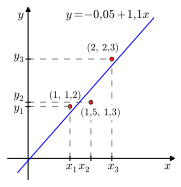
\includegraphics[scale=0.9]{./cap_ajuste/pics/ex_intro_ajuste/ex_intro_ajuste}
  \caption{Exemplo de um problema de ajuste de uma reta entre três pontos, veja o Exemplo~\ref{ex:intro_ajuste}.}
  \label{fig:ex_intro}
\end{figure}

Aqui, o termo ``melhor se ajusta'' é entendido no sentido de mínimos quadrados, isto é, buscamos encontrar uma função $f\in\mathcal{F}$ tal que $f(x)$ resolve o seguinte problema de minimização
\begin{equation}
  \min_{f\in\mathcal{F}} \sum_{j=1}^N \left(f(x_j) - y_j\right)^2,
\end{equation}
ou seja, $f(x)$ é a função da família $\mathcal{F}$ cujo erro quadrático entre $y_j$ e $f(x_j)$, $j = 1, 2, \dotsc, N$, é mínimo. A expressão
\begin{equation}
  \begin{split}
  R &:= \sum_{j=1}^N \left(f(x_j)-y_j\right)^2 \\
  &= \left(f(x_1)-y_1\right)^2 +  \left(f(x_2)-y_2\right)^2 + \cdots + \left(f(x_N)- y_N\right)^2
  \end{split}
\end{equation}
é chamada de \emph{soma do quadrado dos resíduos}\index{resíduo} e consiste na soma dos quadrados das diferenças entre a ordenadas $y_j$ e o valor da função procurada $f(x_j)$.

\begin{ex}\label{ex:intro_ajuste}
  Dado o conjunto de pontos $\{(1, 1,2)$, $(1,5, 1,3)$, $(2, 2,3)\}$ e a família de retas $f(x) = a + bx$, podemos mostrar que $f(x) = -0,05 + 1,1x$ é a reta que melhor aproxima os pontos dados no sentido de mínimos quadrados.  Os pontos e a reta ajustada e são esboçados na Figura~\ref{fig:ex_intro}.
\end{ex}

Na sequência, discutimos o procedimento de ajuste de uma reta, então, mostramos a generalização da técnica para problemas lineares de ajuste e, por fim, discutimos alguns problemas de ajuste não lineares.

%%%%%%%%%%%%%%%%%%%%
% python
%%%%%%%%%%%%%%%%%%%%
\ifispython
  Ao longo deste capítulo, assumiremos que as seguintes bibliotecas e módulos \verb+Python+ estão carregadas:
\begin{verbatim}
>>> import numpy as np
>>> from numpy import linalg
>>> import matplotlib.pyplot as plt
\end{verbatim}
\fi
%%%%%%%%%%%%%%%%%%%%


\section{Ajuste de uma reta}\index{ajuste!de uma reta}

Nesta seção, discutiremos o procedimento de ajuste de uma reta a um conjunto de pontos dados. Em outras palavras, discutiremos o método de solução para o problema de encontrar o polinômio do primeiro grau que melhor se aproxima a um dado conjunto de pontos pelo método dos mínimos quadrados.

Seja, então, $\{(x_1,y_1), (x_2,y_2),\ldots, (x_N,y_N)\}$ um conjunto de $N$ pontos dados. Buscamos encontrar a função $f(x) = a_1 + a_2x$ tal que o resíduo
\begin{equation}
  R = \sum_{j=1}^N (f(x_j)-y_j)^2
\end{equation}
seja mínimo.

Para tal, primeiro observamos que $f(x_j)=a_1+a_2 x_j$ e, portanto, o resíduo pode ser escrito explicitamente como uma função de $a_1$ e $a_2$ conforme a seguinte expressão:
\begin{equation}
  R(a_1,a_2) = \sum_{j=1}^N (a_1 + a_2x_j - y_j)^2.
\end{equation}

%O objetivo é encontrar $a_1, a_2$ e geralmente temos muito mais equações do que incógnitas, isto é,
%\begin{eqnarray}
% a_1+a_2 x_1 &=&y_1 \\
% a_1+a_2 x_2 &=&y_2 \\
% a_1+a_2 x_3 &=&y_3 \\
%  \vdots     &=& \vdots \\
% a_N+a_2 x_N &=&y_N
%\end{eqnarray}
%ou simplesmente $V\vec a= \vec y$.

Observamos que $R(a_1,a_2)$ é uma forma quadrática e que seu mínimo ocorre quando suas derivadas parciais primeiras são iguais a zero, isto é,
\begin{eqnarray}
  \frac{\partial R}{\partial a_1} &=& \frac{\partial }{\partial a_1} \sum_{j=1}^N (a_1 + a_2 x_j-y_j)^2 =0, \\
  \frac{\partial R}{\partial a_2} &=& \frac{\partial }{\partial a_2} \sum_{j=1}^N (a_1 + a_2 x_j-y_j)^2 =0.
\end{eqnarray}
Ou seja,
\begin{eqnarray}
   2 \sum_{j=1}^N (a_1 + a_2 x_j-y_j)\cdot 1 &=&0, \\
   2 \sum_{j=1}^N (a_1 + a_2 x_j-y_j)\cdot x_j &=&0,
\end{eqnarray}
e isolando as incógnitas temos
\begin{eqnarray}
   a_1\sum_{j=1}^N 1 + a_2 \sum_{j=1}^Nx_j &=&\sum_{j=1}^N y_j,\\
   a_1\sum_{j=1}^N x_j + a_2 \sum_{j=1}^Nx_j^2 &=&\sum_{j=1}^N y_jx_j.
\end{eqnarray}
Observando que $\sum_{j=1}^N 1=N$, o sistema linear acima pode ser escrito na forma matricial $Ma = w$, isto é,
\begin{equation}\label{eq:smq_reta}
  \underbrace{\begin{bmatrix}
     N &  \sum_{j=1}^N x_j \\
     \sum_{j=1}^N x_j &  \sum_{j=1}^N x_j^2
  \end{bmatrix}}_{M}
  \underbrace{\begin{bmatrix}
     a_1 \\
     a_2
  \end{bmatrix}}_{a} =
  \underbrace{\begin{bmatrix}
     \sum_{j=1}^N y_j \\
     \sum_{j=1}^N x_j y_j
  \end{bmatrix}}_{w}.
\end{equation}

Este sistema linear de duas equações e duas incógnitas admite uma única solução quando o determinante da matriz dos coeficientes for não nulo, isto é,
\begin{eqnarray}
N \sum_{j=1}^N x_j^2 - \left(\sum_{j=1}^N x_j\right)^2 \neq 0
\end{eqnarray}

Pode-se mostrar usando a \emph{desigualdade de Cauchy–Schwarz} que isto acontece quando existem pelo menos duas abscissas diferentes envolvidas no ajuste.  Usando a fórmula da inversa de uma matriz dois-por-dois, chegamos às seguintes fórmulas para os coeficientes $a_1$ e $a_2$:
  \begin{equation}\label{eq:formula_final_ajuste_reta}
    \begin{split}
    a_1 &= \frac{\sum_{j=1}^N x_j^2  \cdot \sum_{j=1}^N y_j - \sum_{j=1}^N x_j \cdot \sum_{j=1}^N x_jy_j}{N \sum_{j=1}^N x_j^2 - \left(\sum_{j=1}^N x_j\right)^2}\\
    a_2 &= \frac{N \sum_{j=1}^N x_jy_j - \sum_{j=1}^N x_j  \cdot \sum_{j=1}^N y_j }{N \sum_{j=1}^N x_j^2 - \left(\sum_{j=1}^N x_j\right)^2}
    \end{split}
\end{equation}

Por fim, observamos que o sistema $Ma = w$ descrito na Equação~\eqref{eq:smq_reta} pode ser reescrito na forma $V^TVa = V^Ty$, onde $V := [1~x]$ é a matriz dos coeficientes do seguinte sistema linear sobre determinado:
\begin{equation}\label{eq:smq_reta2}
  \begin{split}
  a_1 + a_2x_1 &= y_1\\
  a_1 + a_2x_2 &= y_2\\
  &\vdots\\
  a_1 + a_2x_N &= y_N
  \end{split}
\end{equation}
Se os pontos dados não são colineares, este sistema não tem solução. Mas, sempre que pelo menos duas abscissas foram diferentes, $M = V^TV$ é uma matriz invertível e (veja o Exercício~\ref{exer:smq_reta}), então
\begin{equation}\label{eq:sol_smq_reta}
  a = \left(V^TV\right)^{-1}V^Ty,
\end{equation}
nos fornece a chamada solução por mínimos quadrados do sistema \eqref{eq:smq_reta2}. Note que esta é uma forma de obter os coeficientes $a = (a_1, a_2)$ equivalente àquela dada em \eqref{eq:formula_final_ajuste_reta}.


\begin{ex}\label{ex:calculo_intro_ajuste}
  Retornemos ao Exemplo~\ref{ex:intro_ajuste}. Isto é, dado o conjunto de pontos $\{(1, 1,2)$, $(1,5, 1,3)$, $(2, 2,3)\}$, encontrar a função do tipo $f(x) = a_1 + a_2x$ que melhor se ajusta os pontos dados no sentido de mínimos quadrados.
\end{ex}
\begin{sol} Usando as fórmulas em \eqref{eq:formula_final_ajuste_reta}, obtemos
  \begin{eqnarray}
    a_1&=&\frac{7,25 \cdot 4,8 - 4,5 \cdot 7,75  }{3\cdot 7,25 - 20,25 } = -0,05, \\
    a_2&=&\frac{3\cdot 7,75 - 4,5\cdot 4,8}{3\cdot 7,25 - 20,25}=1,1.
  \end{eqnarray}
Ou seja, verificamos que, de fato, a função $f(x) = -0,05 + 1,1x$ corresponde à reta que melhor ajusta os pontos dados no sentido de mínimos quadrados. Os pontos e a reta ajustada estão esboçados na Figura~\ref{fig:ex_intro}.

Deixamos ao leitor a verificação de que os coeficientes $a_1$ e $a_2$ também podem ser obtidos pela expressão~\eqref{eq:sol_smq_reta}.

%%%%%%%%%%%%%%%%%%%%
% scilab
%%%%%%%%%%%%%%%%%%%%
\ifisscilab
Os coeficientes $a_1$ e $a_2$ podem ser rapidamente calculados no \verb+Scilab+ usando a expressão~\eqref{eq:sol_smq_reta}. Para tanto, digitamos:
\begin{verbatim}
-->xj = [1, 1.5, 2]';
-->yj = [1.2, 1.3, 2.3]';
-->V = [ones(3,1) xj];
-->a = inv(V'*V)*V'*yj
 a  =
  - 0.05
    1.1
\end{verbatim}
Então, o gráfico da função ajustada e dos pontos pode ser obtido com os comandos:
\begin{verbatim}
-->deff('y = f(x)','y = a(1) + a(2)*x')
-->xx = linspace(0.5,2.5);
-->plot(xj,yj,'ro',xx,f(xx),'b-')
\end{verbatim}
\fi
%%%%%%%%%%%%%%%%%%%%
%%%%%%%%%%%%%%%%%%%%
% octave
%%%%%%%%%%%%%%%%%%%%
\ifisoctave
Os coeficientes $a_1$ e $a_2$ podem ser rapidamente calculados no \verb+GNU Octave+ usando a expressão~\eqref{eq:sol_smq_reta}. Para tanto, digitamos:
\begin{verbatim}
xj = [1, 1.5, 2]';
yj = [1.2, 1.3, 2.3]';
V = [ones(3,1) xj];
a = inv(V'*V)*V'*yj
\end{verbatim}
o que nos fornece no {\it prompt}:
\begin{verbatim}
 a  =
  - 0.05
    1.1
\end{verbatim}
Então, o gráfico da função ajustada e dos pontos pode ser obtido com os comandos:
\begin{verbatim}
f = inline("a(1) + a(2)*x")
xx = linspace(0.5,2.5);
plot(xj,yj,'ro',xx,f(xx),'b-');grid on
\end{verbatim}
\fi
%%%%%%%%%%%%%%%%%%%%
%%%%%%%%%%%%%%%%%%%%
% python
%%%%%%%%%%%%%%%%%%%%
\ifispython
Em \verb+Python+, podemos computar os coeficientes $a_1$ e $a_2$ da seguinte forma:
\begin{verbatim}
>>> xi = np.array([1, 1.5, 2])
>>> yi = np.array([1.2,1.3,2.3])
>>> V = np.array([xi**1,xi**0]).transpose();V
array([[ 1. ,  1. ],
       [ 1.5,  1. ],
       [ 2. ,  1. ]])
>>> a = ((np.linalg.inv((V.transpose()).dot(V))).dot(V.transpose())).dot(yi);a
array([ 1.1 , -0.05])
\end{verbatim}
Então, o gráfico da função ajustada e dos pontos pode ser obtido com os comandos:
\begin{verbatim}
>>> xx = np.linspace(0.5,2.5)
>>> plt.plot(xi,yi,'ro',xx,np.polyval(a,xx),'b-')
>>> plt.grid();plt.show()
\end{verbatim}
\fi
%%%%%%%%%%%%%%%%%%%%

\end{sol}

O procedimento apresentado de ajuste de uma reta por mínimos quadrados pode ser generalizado para qualquer família de funções que seja um espaço vetorial de dimensão finita. Problemas de ajuste com tais famílias de funções é o que chamamos de problemas de ajuste linear, os quais exploramos em detalhe na próxima seção.

\subsection*{Exercício resolvido}

\begin{exeresol}\label{exer:smq_reta}
  \begin{enumerate}[a)]
  \item Mostre que o sistema linear $Ma = w$ descrito na Equação~\ref{eq:smq_reta} pode ser reescrito na forma $V^TVa = V^Ty$, onde $V = [1~x]$.
  \item Mostre que $V$, como definido no item a), tem posto igual a 2 quando pelo menos duas abscissas do conjunto de pontos $\{(x_j, y_j)\}_{j=1}^N$ são diferentes. E, portanto, $M = V^TV$ é uma matriz invertível.
  \end{enumerate}
\end{exeresol}
\begin{resol}
    \begin{enumerate}[a)]
    \item Basta observar que
      \begin{equation}
        V^TV = \begin{bmatrix}
          1 & 1 \cdots & 1\\
          x_1 & x_2 & \cdots & x_N
        \end{bmatrix}
        \begin{bmatrix}
          1 & x_1\\
          1 & x_2\\
          \vdots & \vdots\\
          1 & x_N
        \end{bmatrix} =
        \begin{bmatrix}
          N &  \sum_{j=1}^N x_j \\
          \sum_{j=1}^N x_j &  \sum_{j=1}^N x_j^2
        \end{bmatrix} = M
      \end{equation}
      e
      \begin{equation}
        V^Ty = \begin{bmatrix}
          1 & 1 \cdots & 1\\
          x_1 & x_2 & \cdots & x_N
        \end{bmatrix}
        \begin{bmatrix}
          y_1\\
          y_2\\
          \vdots\\
          y_N
        \end{bmatrix} =
        \begin{bmatrix}
          \sum_{j=1}^N y_j \\
          \sum_{j=1}^N x_j y_j
        \end{bmatrix} = w.
      \end{equation}
    \item Sejam $x_i\neq x_j$ duas abscissas diferentes. Então, a $i$-ésima e $j$-ésima linhas na matriz $V$ são linearmente independentes e, portanto, o posto de $V$ é igual a 2. Por fim, $V^TV$ é não singular, pois, se $u$ é tal que $V^TVu = 0$, então
      \begin{equation}
        0 = u^TV^TVu = (Vu)^T(Vu) = (Vu)\cdot (Vu) \Rightarrow Vu = 0.
      \end{equation}
Agora, $Vu = 0$ é uma combinação linear das linhas de $V$ igual a zero, logo $u = 0$, pois as linhas de $V$ são linearmente independentes como mostrado antes. Concluímos que se $V^TVu = 0$, então $u = 0$, isto é, $V^TV$ é não singular.
    \end{enumerate}
\end{resol}


\subsection*{Exercícios}

\begin{exer}
  Sejam dados o conjunto de pontos $\{(0,23, -0,54)$, $(-0,30, -0,54)$, $(0,04, -0,57)\}$. Encontre a função $f(x) = a_1 + a_2x$ que melhor se ajusta no sentido de mínimos quadrados aos pontos dados. Faça, então, um gráfico com os pontos e o esboço da função ajustada.
\end{exer}
\begin{resp}
    $f(x) = -0,55 -0,01x$.
\end{resp}

\begin{exer}
  Seja dado o conjunto de pontos $\{(-0,35, 0,2)$, $(0,15, -0,5)$, $(0,23, 0,54)$, $(0,35, 0,7)\}$. Encontre a função $f(x) = a_1 + a_2x$ que melhor se ajusta no sentido de mínimos quadrados aos pontos dados. Faça, então, um gráfico com os pontos e o esboço da função ajustada.
\end{exer}
\begin{resp}
    $f(x) = 0,19 - 0,47x$.
\end{resp}

\begin{exer}
  Seja dado o conjunto de pontos $\{(-1,94, 1,02)$, $(-1,44, 0,59)$, $(0,93, -0,28)$, $(1,39, -1,04)\}$. Encontre a função $f(x) = a_1 + a_2x$ que melhor se ajusta no sentido de mínimos quadrados aos pontos dados. Então, responda cada item:
  \begin{enumerate}[a)]
  \item Encontre o valor de $f(1)$.
  \item Encontre o valor de $f(0,93)$.
  \item Encontre o valor de $|f(0,93) - (- 0,28)|$.
  \item Encontre o valor do resíduo $R = \sum_{j=1}^N (f(x_j)-y_j)^2$.
  \end{enumerate}
Forneça os valores calculados com $7$ dígitos significativo por arredondamento.
\end{exer}
\begin{resp}
    a)~$-0,6025387$; b)~$-0,5651848$; c)~$0,2851848$; d)~$0,1488041$.
\end{resp}

\section{Ajuste linear geral}\index{ajuste!linear}

O problema geral de ajuste linear consiste em dada uma família $\mathcal{F}$ gerada pelo conjunto de $m$ funções $\{f_1(x), f_2(x), \dotsc, f_m(x)\}$ e um conjunto de $n$ pares ordenados $\{(x_1, y_1)$, $(x_2, y_2)$, $\ldots$, $(x_n, y_n)\}$, calcular os coeficientes $a_1$, $a_2$, $\ldots$, $a_m$ tais que a função dada por
\begin{equation}
  f(x) = \sum_{j=1}^m a_jf_j(x) = a_1f_1(x)+a_2f_2(x)+\ldots+a_mf_m(x)
\end{equation}
minimiza o resíduo
\begin{equation}
  R= \sum_{i=1}^n \left[f(x_i)-y_i\right]^2.
\end{equation}
Aqui, a minimização é feita por todas as possíveis escolhas dos coeficientes $a_1$, $a_2$, $\ldots$, $a_m$.

Com o objetivo de tornar a desenvolvimento mais claro, vamos escrever $R$ como a soma dos resíduos parciais:
\begin{equation}
  R= \sum_{i=1}^n R_i,\quad \text{onde} \quad R_i := \left[f(x_i)-y_i\right]^2.
\end{equation}
Do fato que $f(x_i)=\sum_{j=1}^m a_jf_j(x_i)$, temos que cada resíduo pode ser escrito como
\begin{equation}
  R_i=  \left[\sum_{j=1}^m a_jf_j(x_i)-y_i\right]^2.
\end{equation}

A fim de encontrar o ponto de mínimo, resolvemos o sistema oriundo de igualar a zero cada uma das derivadas parciais de $R$ em relação aos $m$ coeficientes $a_j$, isto é, devemos resolver:
\begin{eqnarray}
\frac{\partial R}{\partial a_1} &=& 2 \sum_{i=1}^n \frac{\partial R_i}{\partial a_1} = 2\sum_{i=1}^n \left[\sum_{j=1}^m a_jf_j(x_i)-y_i\right] f_1(x_i)=0,\\
\frac{\partial R}{\partial a_2} &=& 2 \sum_{i=1}^n \frac{\partial R_i}{\partial a_2}=2\sum_{i=1}^n \left[\sum_{j=1}^m a_jf_j(x_i)-y_i\right] f_2(x_i)=0,\\
&\vdots&\\
\frac{\partial R}{\partial a_m} &=& 2 \sum_{i=1}^n \frac{\partial R_i}{\partial a_m}= 2\sum_{i=1}^n \left[\sum_{j=1}^m a_jf_j(x_i)-y_i\right] f_m(x_i)=0.
\end{eqnarray}

Dividindo cada equação por 2 e escrevendo na forma matricial, obtemos $Ma=w$, onde a matriz $M$ é dada por:
\begin{eqnarray}
M = \begin{bmatrix}
\sum\limits_{i=1}^n f_1(x_i)^2 & \sum\limits_{i=1}^n f_2(x_i) f_1(x_i) & \!\cdots\! & \sum\limits_{i=1}^n f_m(x_i) f_1(x_i)\\
\sum\limits_{i=1}^n f_1(x_i) f_2(x_i)&\sum\limits_{i=1}^n f_2(x_i)^2 & \!\cdots\! & \sum\limits_{i=1}^n f_m(x_i)  f_2(x_i)\\
\sum\limits_{i=1}^n f_1(x_i) f_3(x_i)&\sum\limits_{i=1}^n f_2(x_i)f_3(x_i) & \!\cdots\! & \sum\limits_{i=1}^n f_m(x_i)  f_3(x_i)\\
\vdots & \vdots & \ddots & \vdots\\
\sum\limits_{i=1}^n f_1(x_i) f_m(x_i)&\sum\limits_{i=1}^n f_2(x_i)f_m(x_i) & \!\cdots\! & \sum\limits_{i=1}^n f_m(x_i)  ^2
\end{bmatrix}.
\end{eqnarray}

E os vetores $a$ e $w$ são dados por:
\begin{eqnarray}
a=\left[
\begin{array}{c}
a_1\\
a_2\\
\vdots\\
a_m
\end{array}
\right]\qquad\text{e}\qquad w=\left[\begin{array}{c}
\sum\limits_{i=1}^n f_1(x_i) y_i\\
\sum\limits_{i=1}^n f_2(x_i) y_i\\
\sum\limits_{i=1}^n f_3(x_i) y_i\\
\vdots\\
\sum\limits_{i=1}^n f_m(x_i) y_i
\end{array}
\right].
\end{eqnarray}

Agora, observamos que $M=V^TV$ e $w=V^T y$, onde a matriz $V$ é dada por:
\begin{equation}
  V=\begin{bmatrix}
    f_1(x_1)&f_2(x_1) & \cdots & f_m(x_1)\\
    f_1(x_2)&f_2(x_2) & \cdots & f_m(x_2)\\
    f_1(x_3)&f_2(x_3) & \cdots & f_m(x_3)\\
    \vdots & \vdots & \ddots & \vdots\\
    f_1(x_n)&f_2(x_n) & \cdots & f_m(x_n)
  \end{bmatrix}
\end{equation}
e $y$ é o vetor coluna $y = (y_1, y_2, \dotsc, y_N)$.

Assim, o problema de ajuste se reduz a resolver o sistema linear $Ma=w$, ou $V^TVa = V^T y$. Este sistema linear tem solução única se a matriz $M$ for inversível. O teorema a seguir mostra que isto acontece sempre a matriz $V$ possui posto $m$, ou seja, o número de linhas linearmente independentes for igual ao número de colunas.\footnote{Nota-se que o posto não pode ultrapassar o número de colunas.}


\begin{teo}
A matriz $M=V^TV$ é quadrada de ordem $m$ e é inversível sempre que o posto da matriz $V$ é igual a número de colunas $m$.
\end{teo}
\begin{proof}
Para provar que $M$ é inversível, precisamos mostrar que se $v$ é um vetor de ordem $m$ e $Mv=0$, então $v=0$. Suponha, então, que $Mv=0$, isto é,
$V^TVv=0$. Tomando o produto interno da expressão $V^TVv=0$ com $v$, temos:
\begin{equation} 0=\left<V^TVv,v\right>=\left<Vv,Vv\right>=\|Vv\|^2 \end{equation}
Portanto $Mv=0$ implica obrigatoriamente $Vv=0$. Como o posto de $V$ é igual ao número de colunas, $v$ precisar ser o vetor nulo.
\end{proof}
%\begin{lem}
% A matriz $M=V^TV$ é simétrica.
%\end{lem}
%\begin{proof}
%Isso é facilmente provado pelo seguinte argumento:
%\begin{equation} M^T=(V^TV)^T=(V)^T(V^T)^T=V^TV=M \end{equation}
%\end{proof}

\begin{obs} Este problema é equivalente a resolver pelo métodos dos mínimos quadrados o seguinte sistema linear:
  \begin{equation}
    \begin{bmatrix}
      f_1(x_1)&f_2(x_1) & \cdots & f_m(x_1)\\
      f_1(x_2)&f_2(x_2) & \cdots & f_m(x_2)\\
      f_1(x_3)&f_2(x_3) & \cdots & f_m(x_3)\\
      \vdots & \vdots & \ddots & \vdots\\
      f_1(x_n)&f_2(x_n) & \cdots & f_m(x_n)
    \end{bmatrix}
    \begin{bmatrix}
      a_1\\
      a_2\\
      \vdots\\
      a_m
    \end{bmatrix}
    =\begin{bmatrix}
      y_1\\
      y_2\\
      y_3\\
      \vdots\\
      y_n
    \end{bmatrix}
  \end{equation}
\end{obs}


\begin{obs}O caso de ajuste de um reta para um conjunto de pontos é um caso particular de ajuste linear.\end{obs}

\begin{figure}
  \centering
  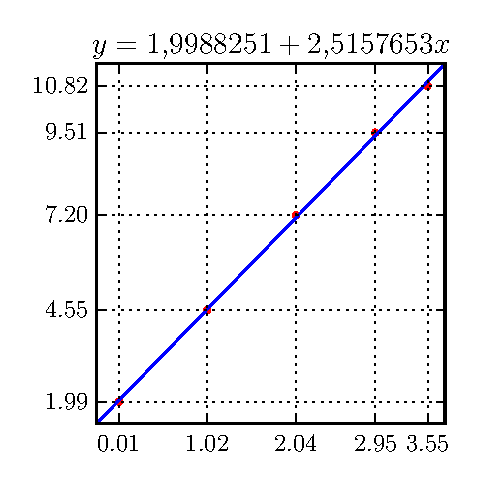
\includegraphics{cap_ajuste/pics/ex_ajuste_reta2/ex_ajuste_reta2}
  \caption{Gráfico da solução do problema apresentado no Exemplo~\ref{ex:ajuste_reta2}.}
  \label{fig:ex_ajuste_reta2}
\end{figure}

\begin{ex}\label{ex:ajuste_reta2} Encontre a reta que melhor se ajusta aos pontos dados na seguinte tabela:
  \begin{center}
    \begin{tabular}{l|ccccc}
      $i$ & $1$   & $2$  & $3$ & $4$ & $5$\\\hline
      $x_i$& $0,01$ & $1,02$ & $2,04$ & $2,95$ & $3,55$\\
      $y_i$ & $1,99$ & $4,55$ & $7,20$ & $9,51$ & $10,82$
    \end{tabular}
  \end{center}
\end{ex}
\begin{sol}
O problema consiste em ajustar uma função da forma $f(x) = a_1 + a_2x$ no conjunto de pontos dados. Notamos que $f(x)$ é uma função da família gerada pelo conjunto de funções $\{f_1(x) = 1, f_2(x) = x\}$. Então, aplicando o procedimento acima, temos que o vetor dos coeficientes $a = (a_1, a_2)$ é solução por mínimos quadrados do sistema linear $Va = y$, onde:
\begin{equation}
  V = \begin{bmatrix}
    f_1(x_1) & f_2(x_1)\\
    f_1(x_2) & f_2(x_2)\\
    f_1(x_3) & f_2(x_3)\\
    f_1(x_4) & f_2(x_4)\\
    f_1(x_5) & f_2(x_5)
  \end{bmatrix}
= \begin{bmatrix}
    1 &0,01\\
    1 &1,02\\
    1 &2,04\\
    1 &2,95\\
    1 &3,55
\end{bmatrix}.
\end{equation}
Ou seja, é a solução do sistema $V^TVa = V^Ty$ dado por
\begin{equation}
  \begin{bmatrix}
    5     & 9,57 \\
    9,57  & 26,5071
  \end{bmatrix}
  \begin{bmatrix}
    a_1   \\
    a_2
  \end{bmatrix}=
  \begin{bmatrix}
    34,07  \\
    85,8144
  \end{bmatrix}
\end{equation}
A solução desse sistema é $a_1 = 1,9988251$ e $a_2 = 2,5157653$. A Figura~\ref{fig:ex_ajuste_reta2}, apresenta um gráfico dos pontos e da reta ajustada.

% A tabela abaixo mostra os valores dados e os valores ajustados:
% \begin{center}
% \begin{tabular}{|c|c|c|c|}
% \hline
% $x_i$ & $y_i$& $ax_i+b$& $ax_i+b-y_i$\\
% \hline
% $0,01$ & $1,99$ & $2,0239828$ & $0,0339828$\\
% $1,02$ & $4,55$ & $4,5649057$ & $0,0149057$ \\
% $2,04$ & $7,2$ & $7,1309863$ & $-0,0690137$ \\
% $2,95$ & $9,51$ & $9,4203327$ & $-0,0896673$  \\
% $3,55$ & $10,82$ & $10,929792$ & $0,1097919$ \\
% \hline
% \end{tabular}
% \end{center}
\end{sol}

\begin{figure}
  \centering
  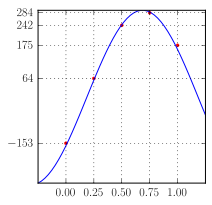
\includegraphics{cap_ajuste/pics/ex_ajuste_linear/ex_ajuste_linear}
  \caption{Gráfico da solução do problema apresentado no Exemplo~\ref{ex:ajuste_linear}.}
  \label{fig:ex_ajuste_linear}
\end{figure}


\begin{ex}\label{ex:ajuste_linear} Encontre a função $f(x)=a_1\sen(\pi x) + a_2\cos(\pi x)$ que melhor se ajusta pelo critérios dos mínimos quadrados aos seguintes pontos dados
  \begin{center}
    \begin{tabular}{l|ccccc}
      $i$ & $1$  & $2$ & $3$ & $4$ & $5$\\\hline
      $x_i$ & $0,00$ & $0,25$ & $0,50$ & $0,75$ & $1,00$\\
      $y_i$ & $-153$ & $64$ & $242$ & $284$ & $175$
    \end{tabular}
  \end{center}
\end{ex}
\begin{sol}
Pelo procedimento visto nesta seção, temos que os coeficientes $a_1$ e $a_2$ são dados pela solução por mínimos quadrados do seguinte sistema linear $Va = y$
\begin{equation}
  \begin{split}
    a_1\sen(\pi x_1) + a_2\cos(\pi x_1) &= y_1\\
    a_1\sen(\pi x_2) + a_2\cos(\pi x_2) &= y_2\\
    a_1\sen(\pi x_3) + a_2\cos(\pi x_3) &= y_3\\
    a_1\sen(\pi x_4) + a_2\cos(\pi x_4) &= y_4\\
    a_1\sen(\pi x_5) + a_2\cos(\pi x_5) &= y_5
  \end{split}
\end{equation}
cuja matriz de coeficientes $V$ é:
\begin{equation}
  V=\begin{bmatrix}
    \sin(0) & \cos(0)  \\
    \sin(0,25\pi) & \cos(0,25\pi)  \\
    \sin(0,5\pi) & \cos(0,5\pi)  \\
    \sin(0,75\pi) & \cos(0,75\pi)  \\
    \sin(\pi) & \cos(\pi)  \\
 \end{bmatrix}
\end{equation}

Então, a solução por mínimos quadrados é
\begin{equation}
  a = (V^TV)^{-1}V^Ty =
  \begin{bmatrix}
    244,03658\\
    -161,18783
  \end{bmatrix}.
\end{equation}
Ou seja, $f(x) = 244,03658\sen(\pi x) - 161,18783\cos(\pi x)$ é a função ajustada ao conjunto de pontos dados. A Figura~\ref{fig:ex_ajuste_linear} apresenta o gráfica de $f(x)$ e dos pontos dados.

%%%%%%%%%%%%%%%%%%%%
% scilab
%%%%%%%%%%%%%%%%%%%%
\ifisscilab
No \verb+Scilab+, podemos computar os coeficientes da função $f(x)$ da seguinte forma:
\begin{verbatim}
-->xi = [0 0.25 0.5 0.75 1]';
-->yi = [-153 64 242 284 175]';
-->V = [sin(%pi*xi) cos(%pi*xi)];
-->a = inv(V'*V)*V'*yi
 a  =
    244.03658
  - 161.18783
\end{verbatim}
\fi
%%%%%%%%%%%%%%%%%%%%
%%%%%%%%%%%%%%%%%%%%
% octave
%%%%%%%%%%%%%%%%%%%%
\ifisoctave
No \verb+GNU Octave+, podemos computar os coeficientes da função $f(x)$ da seguinte forma:
\begin{verbatim}
xi = [0 0.25 0.5 0.75 1]';
yi = [-153 64 242 284 175]';
V = [sin(pi*xi) cos(pi*xi)];
a = inv(V'*V)*V'*yi
\end{verbatim}
o que nos fornece no {\it prompt}:
\begin{verbatim}
a =
   244.04
  -161.19
\end{verbatim}
\fi
%%%%%%%%%%%%%%%%%%%%
%%%%%%%%%%%%%%%%%%%%
% python
%%%%%%%%%%%%%%%%%%%%
\ifispython
Em \verb+Python+, podemos computar os coeficientes da função $f(x)$ da seguinte forma:
\begin{verbatim}
>>> xi = np.array([0,0.25,0.5,0.75,1])
>>> yi = np.array([-153,64,242,284,175])
>>> V = np.array([np.sin(np.pi*xi),np.cos(np.pi*xi)]).transpose()
>>> a = ((np.linalg.inv((V.transpose()).dot(V))).dot(V.transpose())).dot(yi)
\end{verbatim}
\fi
%%%%%%%%%%%%%%%%%%%%

% A tabela abaixo mostra os valores dados e os valores ajustados:
% \begin{center}
% \begin{tabular}{|c|c|c|c|}
% \hline
% $x_i$ & $y_i$& $f(x_i)$& $f(x_i)-y_i$\\
% \hline
% 0  &   -153&  - 161,18783&  -8,1878306 \\
% 0,25&    64 &    58,582912&  -5,4170876 \\
% 0,5 &    242&    244,03658&   2,0365799 \\
% 0,75&    284&    286,53693&   2,5369286 \\
% 1   &    175&    161,18783&  -13,812169 \\
% \hline
% \end{tabular}
% \end{center}
\end{sol}

%%%%%%%%%%%%%%%%%%%%
% scilab
%%%%%%%%%%%%%%%%%%%%
\ifisscilab
\begin{obs}
  No \verb+Scilab+, quando resolvemos um sistema $Ax = b$ usando
\begin{verbatim}
-->x = inv(A)*b
\end{verbatim}
estamos computando a inversa da matriz $A$ e multiplicando por $b$. Podemos evitar a computação da inversa de $A$ usando o operador contra barra (\verb+\+). Neste caso, escrevemos
\begin{verbatim}
-->x = A\b
\end{verbatim}
Quando o sistema $A$ não é uma matriz quadrada, \verb+A\b+ retorna a solução por mínimos quadrados do sistema $Ax = b$, enquanto \verb+inv(A)*b+ retorna um erro, pois $A$ não é uma matriz quadrada e, portanto, não é invertível.
\end{obs}
\fi
%%%%%%%%%%%%%%%%%%%%
%%%%%%%%%%%%%%%%%%%%
% octave
%%%%%%%%%%%%%%%%%%%%
\ifisoctave
\begin{obs}
  No \verb+GNU octave+, quando resolvemos um sistema $Ax = b$ usando
\begin{verbatim}
>> x = inv(A)*b
\end{verbatim}
estamos computando a inversa da matriz $A$ e multiplicando por $b$. Podemos evitar a computação da inversa de $A$ usando o operador contra barra ($/$). Neste caso, escrevemos
\begin{verbatim}
>> x = A/b
\end{verbatim}
Quando o sistema $A$ não é uma matriz quadrada, \verb+A/b+ retorna a solução por mínimos quadrados do sistema $Ax = b$, enquanto \verb+inv(A)*b+ retorna um erro, pois $A$ não é uma matriz quadrada e, portanto, não é invertível.
\end{obs}
\fi
%%%%%%%%%%%%%%%%%%%%
%%%%%%%%%%%%%%%%%%%%
% python
%%%%%%%%%%%%%%%%%%%%
\ifispython
\begin{obs}
  Em \verb+Python+, quando resolvemos um sistema $Ax = b$ usando
\begin{verbatim}
>>> x = np.linalg.inv(A).dot(b)
\end{verbatim}
estamos computando a inversa da matriz $A$ e multiplicando por $b$. Dde forma mais eficiente, podemos usar a função \href{https://docs.scipy.org/doc/numpy/reference/generated/numpy.linalg.solve.html}{numpy.linalg.solve}, digitando:
\begin{verbatim}
>>> x = np.linalg.solve(A,b)
\end{verbatim}
Isto requer que a matriz $A$ seja quadrada e de posto completo. Alternativamente, para obtermos a solução por mínimos quadrados, podemos usar a função \href{https://docs.scipy.org/doc/numpy/reference/generated/numpy.linalg.lstsq.html}{numpy.linalg.lstsq}. Neste caso, digitamos:
\begin{verbatim}
>>> np.linalg.lstsq(A,b)
\end{verbatim}
\end{obs}
\fi
%%%%%%%%%%%%%%%%%%%%

%Observe que é equivalente ao problema matricial
%\begin{equation}
%   Ma := V^TV a = V^Ty
%\end{equation}


% Considere o sistema linear dado por
% $Ax=b$
% onde $A$ é uma matriz $n\times m$ e $b$ é um vetor de $n$ linhas. Assumimos as seguintes hipóteses:
% \begin{itemize}
% \item $n\geq m$. O número de linhas é igual ou superior ao número de colunas. (Mais equações que incógnitas)
% \item O posto de $A$ é $m$, isto é, existem $m$ linhas L.I. Isso implica que $Av=0$ apenas quando $v=0$
% \end{itemize}

% Neste caso, não seremos necessariamente capazes de encontrar um vetor $x$ que satisfaça exatamente a equação $Ax=b$, pelo que estamos interessamos no problema de encontrar o vetor $x$ (ordem m) que minimiza o erro quadrático dado por:
% \begin{equation}\label{defEm}
% E:=\sum_{j=1}^N \left[z_i- b_i\right]^2
% \end{equation}
% onde $z=Ax$ e $z_i$ é linha $i$ do vetor $z$, dado por:
% \begin{equation}\label{Axi}
% z_j=(Ax)_j=\sum_{j=1}^m a_{ij} x_j,\quad j=1,\cdots,n
% \end{equation}
% onde $a_{ij}$ é o elemento de $A$ na linha $i$ e coluna $j$.
% Substituindo (\ref{Axi}) em (\ref{defEm})
% \begin{equation}\label{erro}
% E:=\sum_{j=1}^N \left[\sum_{j=1}^m a_{ij} x_j- b_i\right]^2
% \end{equation}
% Esta é uma função diferenciável nos coeficientes $x_j$ e portanto todo ponto de mínimo acontece quando $\nabla E=0$, ou seja, quando \begin{equation} \frac{\partial}{\partial x_l}E=0,\forall 1\leq l \leq m  \end{equation}

% O que implica a seguinte condição
% \begin{eqnarray}
% 0=\frac{\partial}{\partial x_l}E=\sum_{j=1}^N 2\left[\sum_{j=1}^m a_{ij} x_j- b_i\right] a_{il}, ~~~l=1,\cdots, m
% \end{eqnarray}
% Equivalente a
% \begin{eqnarray}
% \sum_{j=1}^N\sum_{j=1}^m  a_{il}x_j a_{ij}=\sum_{j=1}^Na_{il}b_i,~~~l=1,\cdots, m
% \end{eqnarray}
% que pode ser reescrito na forma vetorial como:
% \begin{eqnarray}\label{cond_vet}
% \left[
% \begin{array}{c}
% \sum_{j=1}^N\sum_{j=1}^m   a_{i1}x_ja_{ij}\\
% \sum_{j=1}^N\sum_{j=1}^m   a_{i2}x_ja_{ij}\\
% \vdots\\
% \sum_{j=1}^N\sum_{j=1}^m   a_{im}x_ja_{ij}\\
% \end{array}
% \right]
% =
% \left[
% \begin{array}{c}
% \sum_{j=1}^Na_{i1}b_i\\
% \sum_{j=1}^Na_{i2}b_i\\
% \vdots\\
% \sum_{j=1}^Na_{im}b_i
% \end{array}
% \right]
% \end{eqnarray}
% Observamos agora que a expressão (\ref{cond_vet}) é equivalente ao seguinte problema matricial:
%
% \begin{equation}\framebox[100 pt][c]{$A^TA x = A^Tb$}\end{equation}

\subsection{Ajuste polinomial}\index{ajuste!polimomial}

O \emph{ajuste polinomial} é o caso particular do ajuste linear para \emph{funções polinomiais}, isto é, funções do tipo
\begin{equation}
  p(x)=a_1 + a_2 x + \cdots + a_{m}x^{m-1}.
\end{equation}

Neste caso, a matriz $V$ associada ao ajuste dos pontos $\{(x_1, y_1)$, $(x_2, y_2)$, $(x_3, y_3)$, $\ldots$, $(x_n,y_n)\}$ é dada por:
\begin{equation}
  V=
\begin{bmatrix}
  1     &    x_1   &   x_1^2& \cdots & x_1^{m-1}\\
  1     &    x_2   &   x_2^2& \cdots & x_2^{m-1}\\
  1     &    x_3   &   x_3^2& \cdots & x_3^{m-1}\\
  \vdots&    \vdots&  & \ddots & \vdots    \\
  1     &    x_n   &   x_n^2& \cdots & x_n^{m-1}
\end{bmatrix}
\end{equation}
Então, os coeficientes $a_i$, $i = 1, 2, \ldots, m$, são dados pela solução do sistema linear $V^TV a = v^Ty$:
\begin{equation}
  \underbrace{\begin{bmatrix}
     n     &  \sum\limits_{j=1}^n  x_j   & \cdots & \sum\limits_{j=1}^n x_j^{m-1}\\
     \sum\limits_{j=1}^n x_j   &  \sum\limits_{j=1}^n  x_j^2 &        & \sum\limits_{j=1}^n x_j^{m}\\
     \vdots     &              & \ddots & \vdots    \\
     \sum\limits_{j=1}^n x_j^{m-1} &  \sum\limits_{j=1}^n  x_j^{m} & \cdots & \sum\limits_{j=1}^n x_j^{2m-1}
  \end{bmatrix}}_{V^TV}
  \underbrace{\begin{bmatrix}
     a_1 \\
     a_2 \\
     \vdots \\
     a_{p+1}
  \end{bmatrix}}_{a}=
  \underbrace{\begin{bmatrix}
     \sum\limits_{j=1}^n y_j \\
     \sum\limits_{j=1}^n x_j y_j \\
     \vdots \\
     \sum\limits_{j=1}^n x_j^{m-1} y_j
  \end{bmatrix}}_{V^Ty}
\end{equation}

\begin{figure}
  \centering
  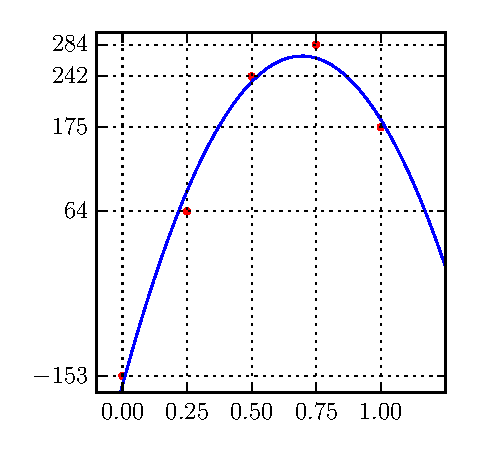
\includegraphics{cap_ajuste/pics/ex_ajuste_polinomial/ex_ajuste_polinomial}
  \caption{Gráfico da solução do problema apresentado no Exemplo~\ref{ex:ajuste_polinomial}.}
  \label{fig:ex_ajuste_polinomial}
\end{figure}


\begin{ex}\label{ex:ajuste_polinomial} Entre o polinômio de grau 2 que melhor se ajusta aos pontos dados na seguinte tabela:
  \begin{center}
    \begin{tabular}{l|ccccc}
      $i$ & $1$ & $2$ & $3$ & $4$ & $5$\\\hline
      $x_i$ & $0,00$ & $0,25$ & $0,50$ & $0,75$ & $1,00$\\
      $y_i$ & $-153$ & $64$ & $242$ & $284$ & $175$
    \end{tabular}
  \end{center}
\end{ex}
\begin{sol}
Um polinômio de grau 2 pode ser escrito na seguinte forma:
\begin{equation}
  p(x) = a_1 + a_2x + a_3x^2.
\end{equation}
Assim, o problema se resume em encontrarmos a solução por mínimos quadrados do seguinte sistema linear:
\begin{equation}
  \begin{split}
  a_1 + a_2x_1 + a_3x_1^2 &= y_1\\
  a_2 + a_2x_2 + a_3x_2^2 &= y_2\\
  a_3 + a_2x_3 + a_3x_3^2 &= y_3\\
  a_4 + a_2x_4 + a_3x_4^2 &= y_4\\
  a_5 + a_2x_5 + a_3x_5^2 &= y_5
  \end{split}
\end{equation}
Ou, escrita na forma matricial, $Va = y$, onde:
\begin{equation}
  V =
  \begin{bmatrix}
    1 & x_1 & x_1^2\\
    1 & x_2 & x_2^2\\
    1 & x_3 & x_3^2\\
    1 & x_4 & x_4^2\\
    1 & x_5 & x_5^2
  \end{bmatrix}
\end{equation}

A solução por mínimos quadrados é, então:
\begin{equation}
  a = (V^TV)^{-1}V^Ty =
  \begin{bmatrix}
    - 165,37143 \\
    1250,9714  \\
  - 900,57143
  \end{bmatrix}
\end{equation}
Ou seja, o polinômio de grau 2 que melhor ajusta os pontos dados no sentido de mínimos quadrados é $p(x) = -165,37143 + 1250,9714x -900,57143x^2$. A Figura~\ref{fig:ex_ajuste_polinomial} mostra o gráfico do polinômio ajustado e os pontos dados.

%%%%%%%%%%%%%%%%%%%%
% scilab
%%%%%%%%%%%%%%%%%%%%
\ifisscilab
No \verb+Scilab+, podemos computar o polinômio $p(x)$ da seguinte forma:
\begin{verbatim}
-->xi = [0 0.25 0.5 0.75 1]';
-->yi = [-153 64 242 284 175]';
-->V = [ones(5,1) xi xi.^2];
-->a = V\yi;
-->p = poly(a,'x','c')
 p  =
                                       2
  - 165.37143 + 1250.9714x - 900.57143x
\end{verbatim}
Para fazermos o gráfico do polinômio e dos pontos, digitamos:
\begin{verbatim}
-->xx = linspace(-0.25,1.25);
-->plot(xi,yi,'ro',xx,horner(p,xx),'b-');xgrid
\end{verbatim}
\fi
%%%%%%%%%%%%%%%%%%%%
%%%%%%%%%%%%%%%%%%%%
% octave
%%%%%%%%%%%%%%%%%%%%
\ifisoctave
No \verb+GNU Octave+, podemos computar o polinômio $p(x)$ da seguinte forma:
\begin{verbatim}
>> xi = [0 0.25 0.5 0.75 1]';
>> yi = [-153 64 242 284 175]';
>> V = [xi.^2 xi xi.^0];
>> a = V\yi
a =

   -900.57
   1250.97
   -165.37
\end{verbatim}
Para fazermos o gráfico do polinômio e dos pontos, digitamos:
\begin{verbatim}
>> xx = linspace(-0.25,1.25);
>> plot(xi,yi,'ro',xx,polyval(a,xx),'b-');grid on
\end{verbatim}
\fi
%%%%%%%%%%%%%%%%%%%%
%%%%%%%%%%%%%%%%%%%%
% python
%%%%%%%%%%%%%%%%%%%%
\ifispython
Em \verb+Python+, podemos computar os coeficientes do polinômio $p(x)$ da seguinte forma:
\begin{verbatim}
>>> xi = np.array([0,0.25,0.5,0.75,1])
>>> yi = np.array([-153,64,242,284,175])
>>> V = np.array([xi**2,xi**1,xi**0]).transpose()
>>> a = ((np.linalg.inv((V.transpose()).dot(V))).dot(V.transpose())).dot(yi)
\end{verbatim}
Para fazermos o gráfico do polinômio e dos pontos, digitamos:
\begin{verbatim}
>>> xx = np.linspace(-0.25,1.25)
>>> plt.plot(xi,yi,'ro',xx,np.polyval(a,xx),'b-')
>>> plt.grid();plt.show()
\end{verbatim}
\fi
%%%%%%%%%%%%%%%%%%%%
\end{sol}

%
% Dado um conjunto de $n$ pontos, desejamos encontrar o \textit{polinômio} de grau $p$ que melhor se ajusta a esses pontos de tal forma a minimizar o resíduo, ou seja, encontrar a curva $f(x)=a_1+a_2 x+...+a_{p+1}x^{p}$ tal que
% \begin{eqnarray}
%   R(a_1,...,a_{p+1}) &=&\sum_{j=1}^N (f(x_j)-y_j)^2 \\
%                  &=&\sum_{j=1}^N (a_1 + a_2 x_j+...+a_{p+1}x_j^p-y_j)^2
% \end{eqnarray}
% seja o menor possível.
%
% O objetivo é encontrar as incógnitas $a_i$ que minimizam a soma do quadrado do resíduo.
%
% O mínimo de $R$ encontra-se quando a derivada primeira é igual a zero:
% \begin{eqnarray}
%   \frac{\partial R}{\partial a_1}     &=& \frac{\partial }{\partial a_1}     \sum_{j=1}^n (a_1 + a_2 x_j+...+a_{p+1}x_j^p-y_j)^2 =0 \\
%   \vdots &=& \vdots \\
%   \frac{\partial R}{\partial a_{p+1}} &=& \frac{\partial }{\partial a_{p+1}} \sum_{j=1}^n (a_1 + a_2 x_j+...+a_{p+1}x_j^p-y_j)^2 =0
% \end{eqnarray}
% ou seja,
% \begin{eqnarray}
%    2 \sum_{j=1}^n (a_1 + a_2 x_j+...+a_{p+1}x_j^p-y_j)\cdot 1    &=&0 \\
%   \vdots &=& \vdots \\
%    2 \sum_{j=1}^n (a_1 + a_2 x_j+...+a_{p+1}x_j^p-y_j)\cdot x_j^p&=&0
% \end{eqnarray}
% e isolando as incógnitas temos
% \begin{eqnarray}
%    a_1\sum_{j=1}^n 1     + a_2 \sum_{j=1}^Nx_j      +...+a_{p+1} \sum_{j=1}^Nx_j^{p} &=\sum_{j=1}^N y_j\\
%   \vdots &= \vdots \\
%    a_1\sum_{j=1}^n x_j^p + a_2 \sum_{j=1}^Nx_j^{p+1}+...+a_{p+1} \sum_{j=1}^Nx_j^{2p} &=\sum_{j=1}^N y_jx_j^{p}
% \end{eqnarray}
%
% Na forma matricial obtemos
% \begin{equation}
%   \begin{bmatrix}
%      \sum 1     &  \sum  x_j   & \cdots & \sum x_j^p\\
%      \sum x_j   &  \sum  x_j^2 &        & \sum x_j^{p+1}\\
%      \vdots     &              & \ddots & \vdots    \\
%      \sum x_j^p &  \sum  x_j^{p+1} & \cdots & \sum x_j^{2p}
%   \end{bmatrix}
%   \begin{bmatrix}
%      a_1 \\
%      a_2 \\
%      \vdots \\
%      a_{p+1}
%   \end{bmatrix}=
%   \begin{bmatrix}
%      \sum y_j \\
%      \sum x_j y_j \\
%      \vdots \\
%      \sum x_j^p y_j
%   \end{bmatrix}
% \end{equation}
%
% Na forma matricial temos
% \begin{equation}
%    Ma := V^TV a = V^Ty
% \end{equation}
%

\subsection*{Exercícios}

\begin{exer}
  Encontre o polinômio $p(x) = a_1 + a_2x + a_3x^2$ que melhor se ajusta no sentido de mínimos quadrados aos pontos:
  \begin{center}
    \begin{tabular}{l|cccc}
      $i$ & $1$ & $2$ & $3$ & $4$ \\\hline
      $x_i$ & $-1,50$ & $-0,50$ & $1,25$ & $1,50$\\
      $y_i$ & $1,15$ & $-0,37$ & $0,17$ & $0,94$
  \end{tabular}
    \end{center}
\end{exer}
\begin{resp}
    $a_1 = -0,67112$, $a_2 = -0,12123$, $a_3 = 0,73907$.
\end{resp}

\begin{exer}Encontrar a parábola $y=ax^2+bx+c$ que melhor aproxima o seguinte conjunto de dados:
  \begin{center}
    \begin{tabular}{l|ccccc}
      $i$ & $1$ & $2$ & $3$ & $4$ & $5$ \\\hline
      $x_i$ & $0,01$ & $1,02$ & $2,04$ & $2,95$ & $3,55$\\
      $y_i$ & $1,99$ & $4,55$ & $7,20$ & $9,51$ & $10,82$
    \end{tabular}
  \end{center}
\end{exer}
\begin{resp}
    $y=-0,0407898x^2+ 2,6613293x+ 1,9364598$.
\end{resp}

\begin{exer} Dado o seguinte conjunto de dados
  \begin{center}
    \begin{tabular}{l|ccccccccccc}
      $x_i$ & $0,0$ & $0,1$ & $0,2$ & $0,3$ & $0,4$ & $0,5$ & $0,6$ & $0,7$ & $0,8$ & $0,9$ & $1,0$\\\hline
      $y_i$ & $31$ & $35$ & $37$ & $33$ & $28$ & $20$ & $16$ & $15$ & $18$ & $23$ & $31$
    \end{tabular}
  \end{center}
\begin{enumerate}[a)]
\item Encontre a função do tipo $f(x)=a+b\sin(2\pi x)+c\cos(2\pi x)$ que melhor aproxima os valores dados.
\item Encontre a função do tipo $f(x)=a+bx+cx^2+dx^3$ que melhor aproxima os valores dados.
\end{enumerate}
\end{exer}
\begin{resp}
    a) $a=25,638625$, $b=9,8591874$, $c=4,9751219$; b)$a=31,475524$, $b=65,691531$, $c=-272,84382$, $d=208,23621$.
\end{resp}



% \begin{exer}Encontre a partir de primeiros princípios a função do tipo $f(x)=bx+a$ que melhor aproxima os pontos:
%   \begin{equation}
%     (0,-0,1), (1,~2), (2,~3,7) ~ \text{e} ~(3,~7).
%   \end{equation}
% \end{exer}
% \begin{resp}
% \begin{eqnarray}
% E_q&=&[f(0)+0,1]^2+[f(1)-2]^2+[f(2)-3,7]^2+[f(3)-7]^2\\
% &=&[a+0,1]^2+[a+b-2]^2+[a+2b-3,7]^2+[a+3b-7]^2
% \end{eqnarray}

% Devemos encontrar os parâmetros $a$ $b$ que minimizam o erro, por isso, calculamos as derivadas parciais:
% \begin{eqnarray}
% \frac{\partial E_q}{\partial a}&=&2[a+0,1]+2[a+b-2]+2[a+2b-3,7]+2[a+3b-7]\\
% \frac{\partial E_q}{\partial b}&=&2[a+b-2]+4[a+2b-3,7]+6[a+3b-7]
% \end{eqnarray}



% O erro mínimo acontece quando as derivadas são nulas, ou seja:
% \begin{eqnarray}
% 8a+12b&=&25,2\\
% 12a+28b&=&60,8
% \end{eqnarray}
% Cuja solução é dada por $a=-0,3$ e $b=2,3$.
% Portanto a função que procuramos é $f(x)=-0,3 +2,3x$.
% \end{resp}



% \begin{exer} Encontre a função do tipo $f(x)=ax$ que melhor se aproxima dos seguintes pontos:
%   \begin{equation}
%     (0, -0,1), (1, 2), (2, 3,7) ~ \text{e} ~(3, 7).
%   \end{equation}
% \end{exer}
% \begin{resp}
% Defina \begin{equation} E_q=[f(x_1)-y_1]^2+[f(x_2)-y_2]^2+[f(x_3)-y_3]^2+[f(x_4)-y_4]^2 \end{equation}
% temos que
% \begin{eqnarray}
% E_q&=&[f(0)+0,1]^2+[f(1)-2]^2+[f(2)-3,7]^2+[f(3)-7]^2\\
% &=&[0,1]^2+[a-2]^2+[2a-3,7]^2+[3a-7]^2
% \end{eqnarray}

% Devemos encontrar o parâmetro $a$ que minimiza o erro, portanto, calculamos:
% \begin{eqnarray}
% \frac{\partial E_q}{\partial a}&=&2[a-2]+4[2a-3,7]+6[3a-7]=28a-60,8
% \end{eqnarray}
% Portanto o valor de $a$ que minimiza o erro é $a=\frac{60,8}{28}$.
% \ifisscilab
% \begin{verbatim}
% x=[0 1 2 3]'
% y=[-.1 2 3.7 7]'
% plot2d(x,y,style=-4)
% \end{verbatim}
% \fi
% \end{resp}


\section{Aproximando problemas não lineares por problemas lineares}

Eventualmente, problemas de ajuste de curvas podem recair em um sistema não linear. Por exemplo, para ajustar função $y=Ae^{bx}$ ao conjunto de pontos $(x_1,y_1)$, $(x_2,y_2)$ e $(x_3,y_3)$, temos que minimizar o resíduo\footnote{A soma do quadrado dos resíduos.}
\begin{equation}
R=(Ae^{x_1b}-y_1)^2+(Ae^{x_2b}-y_2)^2+(Ae^{x_3b}-y_3)^2
\end{equation}
ou seja, resolver o sistema
\begin{eqnarray}
\frac{\partial R}{\partial A} &=& 2(Ae^{x_1b}-y_1)e^{x_1b}+2(Ae^{x_2b}-y_2)e^{x_2b}+2(Ae^{x_3b}-y_3)e^{x_3b}=0\\
\frac{\partial R}{\partial b} &=& 2Ax_1(Ae^{x_1b}-y_1)e^{x_1b} + 2Ax_2(Ae^{x_2b}-y_2)e^{x_2b} \\
&+& 2Ax_3(Ae^{x_3b}-y_3)e^{x_3b}=0
\end{eqnarray}
que é não linear em $A$ e $b$. Esse sistema pode ser resolvido pelo método de Newton-Raphson, o que pode se tornar custoso, ou mesmo inviável quando não dispomos de uma boa aproximação da solução para inicializar o método.

Felizmente, algumas famílias de curvas admitem uma transformação que nos leva a um problema linear. No caso da curva $y=Ae^{bx}$, observe que $\ln y=\ln A+bx$. Assim, em vez de ajustar a curva original $y=Ae^{bx}$ a tabela de pontos, ajustamos a curva submetida a transformação logarítmica
\begin{equation}
  \tilde y:=a_1+a_2 \tilde x=\ln A+bx.
\end{equation}
Usamos os pontos $(\tilde x_j,\tilde y_j):=(x_j,\ln y_j)$, $j=1,2,3$ e resolvemos o sistema linear
\begin{equation}
V^T V \begin{bmatrix} a_1\\a_2\end{bmatrix} = V^T\begin{bmatrix}\tilde{y}_1\\\tilde{y}_2\\\tilde{y}_3\end{bmatrix},
\end{equation}
onde
\begin{equation}
V=\begin{bmatrix} 1&x_1\\1&x_2\\1&x_3 \end{bmatrix}.
\end{equation}

\begin{ex}Encontre uma curva da forma $y=Ae^{bx}$ que melhor ajusta os pontos $(1, 2)$, $(2, 3)$ e $(3, 5)$.
\end{ex}
\begin{sol}
  Aplicando o logaritmo natural de ambos os lados da equação $y=Ae^{bx}$, temos
\begin{equation}
  \ln y = \ln A + bx.
\end{equation}
Então, denotando $\tilde{y} := \ln y$, $a_1 := \ln A$ e $a_2 := b$, o problema reduz-se a ajustar a reta $\tilde{y} = a_1 + a_2x$ aos pontos $(1, \ln 2)$, $(2, \ln 3)$ e $(3, \ln 5)$. Para tanto, resolvemos o sistema
\begin{equation}
  \underbrace{\begin{bmatrix}
    1 & 1\\
    1 & 2\\
    1 & 3
  \end{bmatrix}}_{V}
  \underbrace{\begin{bmatrix}
    a_1\\
    a_2
  \end{bmatrix}}{a} =
  \underbrace{\begin{bmatrix}
    \ln 2\\
    \ln 3\\
    \ln 5
  \end{bmatrix}}_{\tilde{y}}
\end{equation}
por mínimos quadrados, isto é,
\begin{equation}
 V^TVa = V^T\tilde{y} \Rightarrow a = \left(V^TV\right)^{-1}V^T\tilde{y}.
\end{equation}
A solução do sistema é, então, $a_1=0,217442$ e $a_2=0,458145$. Portanto, $A=e^{a_1}=1,24289$ e $b=a_2=0,458145$.

%%%%%%%%%%%%%%%%%%%%
% scilab
%%%%%%%%%%%%%%%%%%%%
\ifisscilab
No \verb+Scilab+, podemos resolver este problema com o seguinte código:
\begin{verbatim}
x = [1 2 3]'
y = [2 3 5]'
V = [ones(3,1) x]
a = V\log(y) //a = inv(V'*V)*V'*log(y)
A = exp(a(1))
b = a(2)
\end{verbatim}
\fi
%%%%%%%%%%%%%%%%%%%%
%%%%%%%%%%%%%%%%%%%%
% octave
%%%%%%%%%%%%%%%%%%%%
\ifisoctave
No \verb+GNU Octave+, podemos resolver este problema com o seguinte código:
\begin{verbatim}
x = [1 2 3]';
y = [2 3 5]';
V = [ones(3,1) x];
a = V\log(y) %a = inv(V'*V)*V'*log(y)
A = exp(a(1))
b = a(2)
\end{verbatim}
\fi
%%%%%%%%%%%%%%%%%%%%
%%%%%%%%%%%%%%%%%%%%
% python
%%%%%%%%%%%%%%%%%%%%
\ifispython
Em \verb+Python+, podemos resolver este problema com o seguinte código:
\begin{verbatim}
x = np.array([1,2,3])
y = np.array([2,3,5])
V = np.array([np.ones(3),x]).transpose()
a = np.linalg.lstsq(V,np.log(y))[0]
A = np.exp(a[0])
b = a[1]
\end{verbatim}
\fi
%%%%%%%%%%%%%%%%%%%%
\end{sol}

\begin{obs}
Os coeficientes obtidos a partir dessa linearização são aproximados, ou seja, são diferentes daqueles obtidos quando aplicamos mínimos quadrados não linear. Observe que estamos minimizando $\displaystyle\sum_i [\ln y_i -\ln (f(x_i))]^2$ em vez de $\displaystyle\sum_i [ y_i -f(x_i)]^2$. No exemplo resolvido, a solução do sistema não linear original seria $A=1,19789$ e $b=0,474348$
\end{obs}

\begin{obs}
Mesmo quando se deseja resolver o sistema não linear, a solução do problema linearizado pode ser usada para construir condições iniciais para o problema não linear.
\end{obs}


A próxima tabela apresenta algumas curvas e transformações que linearizam o problema de ajuste.
\begin{center}
  \begin{tabular}{|c|c|c|}\hline
Curva    & Transformação & Problema Linearizado\\ \hline
$\displaystyle y=ae^{bx}$       & $\tilde y=\ln y$   & $\tilde y=\ln a+ bx$\\
$\displaystyle y=ax^b $       &$\tilde y=\ln y$   & $\tilde y=\ln a+ b\ln x$\\
$\displaystyle y=ax^be^{cx}$    &$\tilde y=\ln y$  & $\tilde y=\ln a+ b\ln x+cx$\\
$\displaystyle y=ae^{(b+cx)^2}$ &$\tilde y=\ln y$       & $\tilde y=\ln a+b^2+ bc x+c^2x^2$\\
$\displaystyle y=\frac{a}{b+x}$ &$\displaystyle \tilde y=\frac{1}{y}$ & $\displaystyle \tilde y=\frac{b}{a}+\frac{1}{a}x$\\
$y=A\cos(\omega x+\phi)$   & $-x-$ &  $y=a\cos(\omega x)-b\sin(\omega x)$ \\
$\omega\ \text{conhecido} $&   &  $a=A\cos(\phi),\ b=A\sin(\phi)$ \\ \hline
  \end{tabular}
\end{center}

\begin{ex}
Encontre a função $f$ da forma $y=f(x)=A\cos(2 \pi x+\phi)$ que ajusta a tabela de pontos
\begin{center}
\begin{tabular}{|c|c|}
\hline
$x_i$ & $y_i$\\
\hline
0,0  &   9,12\\
0,1  &    1,42\\
0,2  &  - 7,76\\
0,3  &  - 11,13\\
0,4  &  - 11,6\\
0,5  &  - 6,44\\
0,6  &    1,41\\
0,7  &    11,01\\
0,8  &    14,73\\
0,9  &    13,22\\
1,0  &    9,93 \\
\hline
\end{tabular}
\end{center}
\end{ex}
\begin{sol}
Usando o fato que $y=A\cos(2 \pi x+\phi)=a\cos(2 \pi x)-b\sin(2 \pi x)$, onde $a=A\cos(\phi)$ e $b=A\sin(\phi)$, $z=[\begin{array}{cc}a &b\end{array}]^T$ é solução do problema
\begin{equation}
B^TBz=B^Ty,
\end{equation}
onde
\begin{equation}
B\!=\!\left[\begin{array}{cc}\cos(2 \pi x_0)& -\sin(2 \pi x_0)\\ \cos(2 \pi x_1)& -\sin(2 \pi x_1)\\ \vdots\\ \cos(2 \pi x_{10})& -\sin(2\pi x_{10}) \end{array}\right]\!=\!\left[\begin{array}{cc}  1.     &      0.\\
    0,8090170 & - 0,5877853\\
    0,3090170 & - 0,9510565\\
  - 0,3090170 & - 0,9510565\\
  - 0,8090170 & - 0,5877853\\
  - 1,0000000 &   0,0000000\\
  - 0,8090170 &   0,5877853\\
  - 0,3090170 &   0,9510565\\
    0,3090170 &   0,9510565\\
    0,8090170 &   0,5877853\\
    1,0000000 &   0,0000000   \end{array}\right].
\end{equation}
Assim, $a=7,9614704$ e $b=11,405721$ e obtemos o seguinte sistema:
\begin{equation}
\left\{\begin{array}{c}
A\cos(\phi)=7,9614704\\ A\sin(\phi)=11,405721
\end{array}\right..
\end{equation}
Observe que
\begin{equation}
A^2=7,9614704^2+11,405721^2
\end{equation}
e, escolhendo $A>0$, $A=13,909546$ e
\begin{equation}
\sin(\phi)=\frac{11,405721}{13,909546}=0,8199923
\end{equation}
Assim, como $\cos\phi$ também é positivo, $\phi$ é um ângulo do primeiro quadrante:
\begin{equation}
\phi=0,9613976
\end{equation}
Portanto $f(x)=13,909546\cos(2\pi x+0,9613976)$. Observe que nesse exemplo a solução do problema linear é a mesma do problema não linear.
\end{sol}

\subsection*{Exercícios resolvidos}

\begin{exeresol}
Encontre a função $f$ da forma $y=f(x)=\frac{a}{b+x}$ que ajusta a seguinte tabela de pontos usando uma das transformações tabeladas.
\begin{center}
  \begin{tabular}{|r|l|l|}
    $i$ & $x_i$ & $y_i$\\\hline
    1 & 0,0 & 101\\
    2 & 0,2 &  85\\
    3 & 0,4 &  75\\
    4 & 0,6 &  66\\
    5 & 0,8 &  60\\
    6 & 1,0 &  55\\\hline
  \end{tabular}
\end{center}
\end{exeresol}
\begin{resol}
Usando o fato que $Y=\frac{1}{y}=\frac{b}{a}+\frac{1}{a}x$, $z=[\begin{array}{cc}\frac{b}{a} &\frac{1}{a}\end{array}]^T$ é solução do problema
\begin{equation}
A^TAz=A^TY,
\end{equation}
onde
\begin{equation}
A=\left[\begin{array}{cc}1& x_1\\ 1& x_2\\ 1&x_3\\1&x_4 \\ 1&x_5 \\ 1&x_6 \end{array}\right]=\left[\begin{array}{cc}
  1 &  0,0\\
  1 &  0,2\\
  1 &  0,4\\
  1 &  0,6\\
  1 &  0,8\\
  1 &  1,0
\end{array}\right]
\end{equation}
e
\begin{equation}
Y=\left[\begin{array}{c}
  1/y_1\\
    1/y_2\\
    1/y_3\\
    1/y_4\\
    1/y_5\\
    1/y_6
\end{array}\right]=\left[\begin{array}{c}
  0,0099010\\
  0,0117647\\
  0,0133333\\
  0,0151515\\
  0,0166667\\
  0,0181818
\end{array}\right]
\end{equation}
Assim, $\frac{1}{a}=0,0082755$ e $\frac{b}{a}=0,0100288$ e, então, $a=120,83924$ e $b=1,2118696$, ou seja, $f(x)=\frac{120,83924}{1,2118696+x}$.
\end{resol}

\subsection*{Exercícios}

\construirExer


%

%ATENÇÃO ESTE CAPITULO
%\include{./cap_derint/cap_derint}
%FOI SEPARADO NOS SEGUINTES

%Este trabalho está licenciado sob a Licença Creative Commons Atribuição-CompartilhaIgual 3.0 Não Adaptada. Para ver uma cópia desta licença, visite https://creativecommons.org/licenses/by-sa/3.0/ ou envie uma carta para Creative Commons, PO Box 1866, Mountain View, CA 94042, USA.

\chapter{Derivação numérica}\index{derivação}

Nesta seção, trataremos das estratégias numéricas para aproximação de derivadas de funções reais. Com as técnicas abordadas, é possível calcular aproximadamente a derivada de uma função a partir de um conjunto discreto de pontos $\{(x_i, y_i)\}_{i=1}^n$. Começamos discutindo as chamadas \emph{aproximações por diferenças finitas}\index{aproximações por diferenças finitas} e, então, as aproximações de derivadas via ajuste ou interpolação.

%%%%%%%%%%%%%%%%%%%%
% python
%%%%%%%%%%%%%%%%%%%%
\ifispython
Ao longo deste capítulo, assumiremos que as seguintes bibliotecas e módulos \verb+Python+ estão importados:
\begin{verbatim}
import numpy as np
import matplotlib.pyplot as plt
\end{verbatim}
\fi
%%%%%%%%%%%%%%%%%%%%

\section{Diferenças finitas}\index{diferenças finitas}

Uma diferença finita é uma expressão da forma $f(x+b)-f(x+a)$, que ao ser dividida por $(b-a)$ chama-se um quociente de diferenças. A técnica de \emph{diferenças finitas}\index{diferenças finitas} consiste em aproximar a derivada de uma função via fórmulas discretas que requerem apenas um conjunto finito de pares ordenados $\left\{\left(x_i, y_i\right)\right\}_{i=1}^n$, onde geralmente denotamos $y_i=f(x_i)$.

Essas fórmulas podem ser obtidas de várias maneiras. Começamos com a fórmula mais simples que pode ser obtida do cálculo diferencial. Seja $f$ uma função diferenciável, a derivada de $f$ no ponto $x_0$ é, por definição,
\begin{equation}
  f'(x_0)=\lim_{h\to 0}\frac{f(x_0+h)-f(x_0)}{h}.
\end{equation}
Deste limite, tomando $h\neq 0$ pequeno (não muito pequeno para evitar o cancelamento catastrófico), é esperado que possamos obter uma aproximação razoável para $f'(x_0)$. Assim, a \emph{diferença finita progressiva} de ordem 1
\begin{equation}\label{eq:dp}
  D_{+,h}f(x_0) := \frac{f(x_0+h)-f(x_0)}{h} \approx f'(x_0)
\end{equation}
é uma aproximação para $f'(x_0)$.

\begin{ex}\label{ex:dp}
Usando a diferença finita progressiva de ordem 1, calcule aproximações da derivada de $f(x)=\cos(x)$ no ponto $x=1$ usando $h=10^{-1}$, $10^{-2}$, $10^{-3}$, $10^{-4}$, $10^{-12}$ e $10^{-14}$. Calcule o erro $|D_{+,h}f(1)-f'(1)|$ obtido para cada valor de $h$.
\end{ex}
\begin{sol}
Usando a diferença progressiva em ~\eqref{eq:dp}, devemos calcular
\begin{equation}
  D_{+,h}f(1) = \frac{\cos(1 + h) - \cos(1)}{h}
\end{equation}
Fazendo isso, obtemos:
\begin{center}
  \begin{tabular}{r|c|c}
    $h$        & $D_{+,h}f(1)$   & $|f'(1) - D_{+,h}f(1)|$ \\ \hline
    $10^{-1}$  & $-8,67062\E-01$ & $2,55909\E-02$\\
    $10^{-2}$  & $-8,44158\E-01$ & $2,68746\E-03$\\
    $10^{-3}$  & $-8,41741\E-01$ & $2,70011\E-04$\\
    $10^{-4}$  & $-8,41498\E-01$ & $2,70137\E-05$ \\
    $10^{-12}$ & $-8,41549\E-01$ & $7,80679\E-05$\\
    $10^{-14}$ & $-8,43769\E-01$ & $2,29851\E-03$ \\\hline
  \end{tabular}
\end{center}

%%%%%%%%%%%%%%%%%%%%
% scilab
%%%%%%%%%%%%%%%%%%%%
\ifisscilab
No \verb+Scilab+, podemos calcular a aproximação da derivada $f'(1)$ com $h=0,1$ usando as seguintes linhas de código:
\begin{verbatim}
--> deff('y = f(x)','y = cos(x)')
--> x0 = 1
--> h  = 0.1
--> df = (f(x0+h) - f(x0))/h
\end{verbatim}
E, similarmente, para outros valores de $x_0$ e $h$.
\fi
%%%%%%%%%%%%%%%%%%%%
%%%%%%%%%%%%%%%%%%%%
% octave
%%%%%%%%%%%%%%%%%%%%
\ifisoctave
No \verb+GNU Octave+, podemos calcular a aproximação da derivada $f'(1)$ com $h=0,1$ usando as seguintes linhas de código:
\begin{verbatim}
f = @(x) cos(x);
x0 = 1;
h = 0.1;
df = (f(x0+h) - f(x0))/h
\end{verbatim}
E, similarmente, para outros valores de $x_0$ e $h$.
\fi
%%%%%%%%%%%%%%%%%%%%
%%%%%%%%%%%%%%%%%%%%
% python
%%%%%%%%%%%%%%%%%%%%
\ifispython
Em \verb+Python+, podemos calcular a aproximação da derivada $f'(1)$ com $h=0,1$ usando as seguintes linhas de código:
\begin{verbatim}
>>> def f(x):
...    return np.cos(x)
...
>>> x0=1
>>> h=0.1
>>> df = (f(x0+h)-f(x0))/h
\end{verbatim}
E, similarmente, para outros valores de $x_0$ e $h$.
\fi
%%%%%%%%%%%%%%%%%%%%
\end{sol}

\begin{figure}
  \centering
  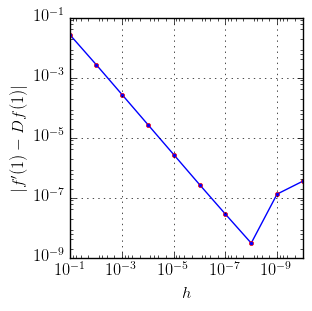
\includegraphics{./cap_derivacao/pics/ex_derivacao/ex_derivacao}
  \caption{Erro absoluto das derivadas numéricas no Exemplo~\ref{ex:dp}.}
  \label{fig:ex_derivacao}
\end{figure}

Exploremos o Exemplo~\ref{ex:dp} um pouco mais. Observamos que, para valores moderados de $h$, o erro $|f'(1)-D_{+,h}f(1)|$ diminui linearmente com $h$ (veja Figura~\ref{fig:ex_derivacao}). Isto é consequência da ordem de truncamento da fórmula de diferenças finitas aplicada (que é de ordem 1). Porém, para valores muito pequenos de $h < 10^{-8}$, o erro passa a aumentar quando diminuímos $h$. Isto é devido ao efeito de cancelamento catastrófico.

\subsection{Diferenças finitas via série de Taylor}

Podemos construir fórmulas de diferenças finitas para uma função $f(x)$ (suave\footnote{Uma função suave é uma função infinitamente continuamente diferenciável, isto é, $f\in C^\infty(\mathbb{R})$. Uma análise mais cuidadosa, revela que hipóteses mais fracas podem ser assumidas.}) no ponto $x = x_0$ a partir de seu polinômio de Taylor. Em alguns casos, este procedimento acaba por nos fornecer, também, a ordem de truncamento da fórmula.

\subsubsection{Diferença finita progressiva de ordem 1}\index{diferenças finitas!progressiva}
Podemos obter uma aproximação para $f'(x_0)$ a partir da série de Taylor
\begin{equation}
  f(x_0+h) = f(x_0) + hf'(x_0) + h^2\frac{f''(\xi)}{2},\quad h>0, \xi\in(x_0,x_0+h).
\end{equation}
Isolando $f'(x_0)$, obtemos
\begin{equation}\label{eq:dp_trunc}
  f'(x_0) = \underbrace{\frac{f(x_0+h) - f(x_0)}{h}}_{D_{+,h}} - \underbrace{h\frac{f''(\xi)}{2}}_{\mathcal{O}(h)},
\end{equation}
o que mostra que o erro de truncamento da \emph{diferença finita progressiva}\footnote{Também chamada de diferença finita progressiva de dois pontos ou diferença para frente.}
\begin{equation}
  D_{+,h}f(x_0) := \frac{f(x_0+h)-f(x_0)}{h}
\end{equation}
é de ordem $h$.

\subsubsection{Diferença finita regressiva de ordem 1}\index{diferenças finitas!regressiva}
Outra aproximação para a derivada primeira pode ser obtida da série de Taylor de $f$ em torno de $(x_0-h)$ dada por
\begin{equation}
  f(x_0-h) = f(x_0) - hf'(x_0) + h^2\frac{f''(\xi)}{2},\quad h>0, \xi\in(x_0, x_0+h).
\end{equation}
Isolando $f'(x_0)$, obtemos
\begin{equation}
  f'(x_0) = \underbrace{\frac{f(x_0) - f(x_0-h)}{h}}_{D_{-,h}} + \underbrace{h\frac{f''(\xi)}{2}}_{\mathcal{O}(h)}.
\end{equation}
que fornece a \emph{diferença finita regressiva}\footnote{Também chamada de diferença regressiva de dois pontos ou diferença para trás.}
\begin{equation}
  D_{-,h}f(x_0) := \frac{f(x_0)-f(x_0-h)}{h},
\end{equation}
que possui erro de truncamento de ordem $h$.

\subsubsection{Diferença finita central de ordem 2}\index{diferenças finitas!central}
Para obter uma aproximação para a derivada primeira com um erro menor, podemos utilizar as séries de Taylor:
\begin{eqnarray}
    f(x_0+h) &= f(x_0) + hf'(x_0) + h^2f''(x_0) + h^3\frac{f'''(\xi_{+})}{3!},\\
    f(x_0-h) &= f(x_0) - hf'(x_0) + h^2f''(x_0) + h^3\frac{f'''(\xi_{-})}{3!}
\end{eqnarray}
Fazendo a primeira equação menos a segunda, obtemos
\begin{equation}
  f(x_0+h)-f(x_0-h) = 2hf'(x_0) + h^{3}\left(\frac{f'''(\xi_{+}) - f'''(\xi_{-})}{3!}\right).
\end{equation}
Dividindo por $2h$ e isolando $f'(x_0)$ obtemos
\begin{equation}
  f'(x_0) = \underbrace{\frac{f(x_0+h) - f(x_0-h)}{2h}}_{D_{0,h}} - \underbrace{h^2\left(\frac{f'''(\xi_+) - f'''(\xi_-)}{2\cdot 3!}\right)}_{\mathcal{O}(h^2)}.
\end{equation}
Assim, a \emph{diferença finita central}\footnote{Também chamada de diferença finita central de três pontos. Note que o ponto $f(x_0)$ possui coeficiente $0$, por isso $3$ pontos.}
\begin{equation}
  D_{0,h}f(x_0) := \frac{f(x_0+h)-f(x_0-h)}{2h},
\end{equation}
é uma aproximação para $f'(x_0)$ com erro de truncamento de ordem $h^2$, ou simplesmente ordem $2$.

\begin{ex}\label{ex:derivacao2}
Calcule a derivada numérica da função $f(x)=e^{\frac{1}{2}x}$ no ponto $x=2$ usando a diferença progressiva, diferença regressiva e diferença central com $h=10^{-1}$, $h=10^{-2}$ e $h=10^{-4}$. Também, calcule o erro absoluto da aproximação obtida em cada caso.
\end{ex}
\begin{sol}
  Usando a diferença progressiva, devemos calcular
  \begin{equation}
    D_{+,h} = \frac{f(x+h) - f(x)}{h} = \frac{e^{\frac{1}{2}(x+h)} - e^{\frac{1}{2}x}}{h}.
  \end{equation}
  Com a diferença regressiva, calculamos
  \begin{equation}
    D_{-,h} = \frac{f(x) - f(x-h)}{h} = \frac{e^{\frac{1}{2}x} - e^{\frac{1}{2}(x-h)}}{h}.
  \end{equation}
  Por fim, usando a diferença central temos
  \begin{equation}
    D_{0,h} = \frac{f(x+h) - f(x-h)}{2h} = \frac{e^{\frac{1}{2}(x+h)} - e^{\frac{1}{2}(x-h)}}{2h}.
  \end{equation}

  As aproximações e os erros absolutos calculados em cada caso estão apresentados na seguinte tabela:
  \begin{center}
    \begin{tabular}{r|cc|cc|cc}
      $h$  & $D_{+,h}f(2)$ & Erro & $D_{-,h}$ & Erro & $D_{0,h}$ & Erro \\\hline
      $10^{-1}$ & $1,39369$ & $3,5\E-02$   & $1,32572$ & $3,3\E-02$ & $1,35971$ & $5,7\E-04$\\
      $10^{-2}$ & $1,36254$ & $3,4\E-03$   & $1,35575$ & $3,4\E-03$ & $1,35915$ & $5,7\E-06$\\
      $10^{-4}$ & $1,35917$ & $3,4\E-05$   & $1,35911$ & $3,4\E-05$ & $1,35914$ & $5,7\E-10$\\\hline
    \end{tabular}
  \end{center}
\end{sol}

\begin{figure}
  \centering
  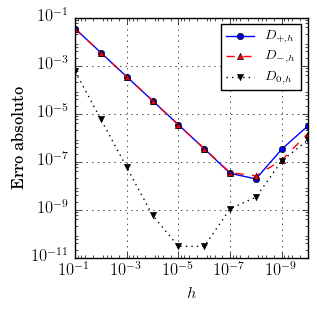
\includegraphics{./cap_derivacao/pics/ex_derivacao2/ex_derivacao2}
  \caption{Erro absoluto das derivadas numéricas no Exemplo~\ref{ex:derivacao2}.}
  \label{fig:ex_derivacao2}
\end{figure}


\begin{obs}
  O experimento numérico realizado no Exemplo~\ref{ex:derivacao2}, nos mostra que o erro absoluto na derivação numérica não é da ordem do erro de truncamento. Entretanto, este erro tende a variar com $h$ na mesma ordem do erro de truncamento. A Figura~\ref{fig:ex_derivacao2} apresenta o erro absoluto das derivadas numéricas computadas para o Exemplo~\ref{ex:derivacao2}. Note que, devido ao efeito de cancelamento catastrófico, o erro absoluto deixa de variar na ordem do erro de truncamento para valores muito pequenos de $h$.
\end{obs}

% \subsection{Erros de truncamento}\index{erros!truncamento}
% Seja $D_{+,h}f(x_0)$ a aproximação da derivada de $f$ em $x_0$ por diferenças progressivas, $D_{-,h}f(x_0)$ a aproximação por diferenças regressivas e $D_{0,h}f(x_0)$ a aproximação por diferenças centrais, então
% \begin{eqnarray}
% D_{+,h}f(x_0)-f'(x_0)&=&\frac{f(x_0+h)-f(x_0)}{h}-f'(x_0)\\
% &=&\frac{f(x_0)+hf'(x_0)+\frac{h^2}{2}f''(x_0)+\mathcal{O}(h^3)-f(x_0)}{h}-f'(x_0)\\
% &=&\frac{h}{2}f''(x_0)+\mathcal{O}(h^2)=\mathcal{O}(h).\\
% \end{eqnarray}
% Analogamente:
% \begin{eqnarray}
% D_{-,h}f(x_0)-f'(x_0)&=&\frac{f(x_0)-f(x_0-h)}{h}-f'(x_0)\\
% &=&\frac{f(x_0)-\left(f(x_0)-hf'(x_0)+\frac{h^2}{2}f''(x_0)+\mathcal{O}(h^3)\right)}{h}-f'(x_0)\\
% &=&-\frac{h}{2}f''(x_0)+\mathcal{O}(h^2)=\mathcal{O}(h).\\
% \end{eqnarray}
% Também:
% \begin{eqnarray}
% D_{0,h}f(x_0)-f'(x_0)&=& \frac{f(x_0+h)-f(x_0-h)}{2h}-f'(x_0)\\
% &=& \frac{f(x_0)+hf'(x_0)+\frac{h^2}{2}f''(x_0)+\mathcal{O}(h^3)}{2h} \\
% &-& \frac{f(x_0)-hf'(x_0)+\frac{h^2}{2}f''(x_0)+\mathcal{O}(h^3)}{2h}-f'(x_0)\\
% &=& \mathcal{O}(h^2).
% \end{eqnarray}

\begin{ex}
Estime o erro absoluto no cálculo da derivada de $f(x)=e^{-x}$ para $x>0$ utilizando a diferença progressiva.
\end{ex}
\begin{sol}
Da Equação~\ref{eq:dp_trunc}, temos:
\begin{equation}
  f'(x) = D_{+,h}f(x) - h\frac{f''(\xi)}{2},\quad \xi>0,
\end{equation}
ou seja:
\begin{equation}
  |f'(x) - D_{+,h}f(x)| = \left|\frac{f''(\xi)}{2}\right|h,\quad \xi>0.
\end{equation}
Agora, como $|f''(x)| = |e^{-x}| < 1$ para $x>0$, concluímos que:
\begin{equation}
  |f'(x) - D_{+,h}f(x)| \leq \frac{1}{2}h,\quad x>0.
\end{equation}
\end{sol}

\subsection{Erros de arredondamento}\index{erros!arredondamento}
Para entender como os erros de arredondamento se propagam ao calcular as derivadas numéricas vamos analisar a fórmula de diferenças finitas progressiva
\begin{equation}
  D_{+,h}f(x) =\frac{f(x+h)-f(x)}{h}.  
\end{equation}

Nesse contexto temos o valor exato $f'(x)$ para a derivada, a sua aproximação numérica $D_{+,h}f(x)$ e a representação em número de máquina do operador $D_{+,h}f(x)$ que denotaremos por $\overline{D_{+,h}f(x)}$. Denotando por $\varepsilon(x,h)$ o erro de arredondamento ao calcularmos a derivada, vamos assumir que
\begin{equation}\label{ex:ea_dp}
\overline{D_{+,h}f(x)}=D_{+,h}f(x)(1+\varepsilon(x,h))=\frac{\overline{f(x+h)}-\overline{f(x)}}{h}(1+\varepsilon(x,h)).  
\end{equation}
Também, consideremos
\begin{equation}
|\overline{f(x+h)}-f(x+h)|=\delta(x,h)\leq \delta  
\end{equation}
e
\begin{equation}
  |\overline{f(x)}-f(x)|=\delta(x,0)\leq \delta,  
\end{equation}
onde $\overline{f(x+h)}$ e $\overline{f(x)}$ são as representações em ponto flutuante dos números $f(x+h)$ e $f(x)$, respectivamente. 

Então, da Equação~\eqref{ex:ea_dp}, a diferença do valor da derivada e sua aproximação representada em ponto flutuante pode ser estimada por:
\begin{equation}
\left|f'(x)-\overline{D_{+,h}f(x)}\right| = \left| f'(x)-\frac{\overline{f(x+h)}-\overline{f(x)}}{h}(1+\varepsilon(x,h)) \right|.
\end{equation}
Podemos reescrever o lado direito desta equação, da seguinte forma
\begin{eqnarray}
  \left|f'(x)-\overline{D_{+,h}f(x)}\right| &=& \left| f'(x)-\left(\frac{\overline{f(x+h)}-\overline{f(x)}}{h}+\frac{f(x+h)-f(x+h)}{h}\right.\right. \\
                                            &+& \left.\left.\frac{f(x)-f(x)}{h}\right)(1+\varepsilon) \right|\\
                                            &=& \left| f'(x)+\left(-\frac{f(x+h)-f(x)}{h}-\frac{\overline{f(x+h)}-f(x+h)}{h}\right.\right.\\
                                            &+& \left.\left. \frac{\overline{f(x)}-f(x)}{h}\right)(1+\varepsilon) \right|.
\end{eqnarray}
Então, separando os termos e estimando, obtemos:
\begin{eqnarray}
\left|f'(x)-\overline{D_{+,h}f(x)}\right| &\leq& \left|f'(x)-\frac{f(x+h)-f(x)}{h}\right| +\left(\left|\frac{\overline{f(x+h)}-f(x+h)}{h}\right|\right.\\
&+&\left.\left|\frac{\overline{f(x)}-f(x)}{h}\right| \right)|1+\varepsilon| + \left|\frac{f(x+h)-f(x)}{h}\right|\varepsilon\\
&\leq& Mh +\left(\left|\frac{\delta}{h}\right|+\left|\frac{\delta}{h}\right| \right)|1+\varepsilon| +|f'(x)|\varepsilon\\
&\leq& Mh +\left(\frac{2\delta}{h}\right)|1+\varepsilon| +|f'(x)|\varepsilon
\end{eqnarray}
onde
\begin{equation}
M=\frac{1}{2}\max_{x\leq y\leq x+h}|f''(y)|
\end{equation}
está relacionado com o erro de truncamento.

Por fim, obtemos a seguinte estimativa para o erro absoluto na computação da derivada numérica:
\begin{equation}\label{eq:est_erro_arredondamento}
  \left|f'(x)-\overline{D_{+,h}f(x)}\right| \leq Mh +\left(\frac{2\delta}{h}\right)|1+\varepsilon| +|f'(x)|\varepsilon.
\end{equation}

Esta estimativa mostra que se o valor de $h$ for muito pequeno o erro ao calcular a aproximação numérica cresce. Isso nos motiva a procurar o valor ótimo de $h$ que minimiza o erro.

\begin{ex}
No Exemplo~\ref{ex:derivacao2}, computamos a derivada numérica da função $f(x)=e^{\frac{1}{2}x}$ no ponto $x=2$ usando as fórmulas de diferenças finitas progressivas, regressivas e central. A Figura~\ref{fig:ex_derivacao2}, mostra que, para valores $h$ muito pequenos, os erros de arredondamento passam a dominar os cálculos e, por consequência, o erro da derivada numérica passa a aumentar. Pela figura, podemos inferir que a escolha ótima de $h$ para as fórmulas progressiva e regressivas é $h\approx 10^{-7}$. Agora, para a fórmula central, $h\approx 10^{-5}$ parece ser a melhor escolha.
\end{ex}

\begin{obs}
  Note que a estimativa~\eqref{eq:est_erro_arredondamento}, mostra que o erro na computação da derivada numérica depende da função que está sendo derivada. Assim, o $h$ ótimo depende não somente da fórmula de diferenças finitas, mas também da função a ser derivada.
\end{obs}

\subsection*{Exercícios resolvidos}

\construirExeresol

\begin{exeresol}
Aproxime a derivada de $f(x)=\sen(2x) - x^2$ no ponto $x=2$ usando a fórmula de diferenças finitas progressiva de ordem 1 com: a) $h=0,1$ e b) $h=0,01$. Compute, também, o erro absoluto de cada aproximação computada.
\end{exeresol}
\begin{resol}
  A fórmula de diferenças finitas de ordem 1 para uma função $y = f(x)$ em um ponto $x = x_0$ é dada por:
  \begin{equation}
    D_{+,h}f(x_0) = \frac{f(x_0+h) - f(x_0)}{h}.
  \end{equation}
Substituindo $f(x) = \sen(2x) - x^2$ e $x_0 = 2$, obtemos:
  \begin{equation}
    \begin{split}
      D_{+,h}f(x_0) &= \frac{(\sen(2(x_0+h)) - (x_0+h)^2) - (\sen(2x_0) - x_0^2)}{h}\\
      &= \frac{\sen(2(x_0+h)) - x_0^2 + 2x_0h + h^2 - \sen(2x_0) + x_0^2)}{h}\\
      &= \frac{\sen(4+2h) + 4h + h^2 - \sen(4))}{h}.
    \end{split}
  \end{equation}
Então, tomando $h=0,1$, podemos computar a derivada numérica e o erro associado:
\begin{equation}
  D_{+,0,1}f(2) = -5,247733,\quad |f'(2)-D_{+,0,1}f(2)| = 5,96\times 10^{-2},
\end{equation}
onde $f'(x) = 2\sen(2x) - 2x$ é a derivada analítica. Tomando $h=0,01$ temos:
\begin{equation}
  D_{+,0,1}f(2) = -5,302065,\quad |f'(2)-D_{+,0,1}f(2)| = 5,22\times 10^{-3}.
\end{equation}

%%%%%%%%%%%%%%%%%%%%
% Scilab
%%%%%%%%%%%%%%%%%%%%
\ifisscilab
\construirScilab
\fi
%%%%%%%%%%%%%%%%%%%%
%%%%%%%%%%%%%%%%%%%%
% GNU octave
%%%%%%%%%%%%%%%%%%%%
\ifisoctave
No \verb+GNU Octave+, podemos fazer os cálculos com o seguinte código:
\begin{verbatim}
#funcao
f = @(x) sin(2*x) - x^2;

#derivada analitica
fl = @(x) 2*cos(2*x) - 2*x;

#d.f. progressiva de ordem 1
dp1 = @(f,x,h=0.1) (f(x+h)-f(x))/h;

#h=0.1
dy = dp1(f,2)
printf("D.F. Progressiva de ordem 1 com h = %f\n", 1e-1)
printf("Df = %f\n", dy)
printf("Erro = %1.2e\n", abs(fl(2)-dy))

#h=0.01
dy = dp1(f,2,1e-2)
printf("D.F. Progressiva de ordem 1 com h = %f\n", 1e-2)
printf("Df = %f\n", dy)
printf("Erro = %1.2e\n", abs(fl(2)-dy))
\end{verbatim}
\fi
%%%%%%%%%%%%%%%%%%%%
%%%%%%%%%%%%%%%%%%%%
% python
%%%%%%%%%%%%%%%%%%%%
\ifispython
Em \verb+Python+, podemos fazer os cálculos com o seguinte código:
\begin{verbatim}
#funcao
def f(x):
    return np.sin(2*x) - x**2

#derivada analitica
def fl(x):
    return 2*np.cos(2*x) - 2*x

#d.f. progressiva de ordem 1
def dp1(f,x,h=0.1):
    return (f(x+h)-f(x))/h

#h=0.1
dy = dp1(f,2)
print("D.F. Progressiva de ordem 1 com h = %f" % 1e-1)
print("Df = %f" % dy)
print("Erro = %1.2e" % np.abs(fl(2)-dy))

#h=0.01
dy = dp1(f,2,1e-2)
print("D.F. Progressiva de ordem 1 com h = %f" % 1e-2)
print("Df = %f" % dy)
print("Erro = %1.2e" % np.abs(fl(2)-dy))
\end{verbatim}
\fi
%%%%%%%%%%%%%%%%%%%%
\end{resol}


\subsection*{Exercícios}

\begin{exer}
Use os esquemas numéricos de diferença finita regressiva de ordem 1, diferença finita progressiva de ordem 1 e diferença finita central de ordem 2 para aproximar as seguintes derivadas:
\begin{itemize}
\item[a)] $f'(x)$ onde $f(x)=\sen(x)$ e $x=2$.
\item[b)] $f'(x)$ onde $f(x)=e^{-x}$ e $x=1$.
\end{itemize}
Use $h=10^{-2}$ e $h=10^{-3}$ e compare com os valores obtidos através da avaliação numérica das derivadas exatas.
\end{exer}
\begin{resp}
  \begin{itemize}
\item[a)] $f'(x)$ onde $f(x)=\sen(x)$ e $x=2$ para $h=10^{-2}$ e $h=10^{-3}$, respectivamente.
\subitem Progressiva ordem 1: $-0,42069$ e $-0,41660$.
\subitem Regressiva ordem 1: $-0,41159$ e $-0,41569$.
\subitem Central ordem 2: $-0,41614$ e $-0,41615$.
\subitem Exata: $\cos(2)=-0,41615$
\item[b)] $f'(x)$ onde $f(x)=e^{-x}$ e $x=1$ para $h=10^{-2}$ e $h=10^{-3}$, respectivamente.
\subitem Progressiva ordem 1: $-0,36605$ e $-0,36788$.
\subitem Regressiva ordem 1: $-0,36972$ e $-0,36806$.
\subitem Central ordem 2: $-0,36789$ e $-0,36788$.
\subitem Exata: $-e^{-1}=-0,36788$
  \end{itemize}
 \end{resp}


\begin{exer}\label{ex1} Expanda a função suave $f(x)$ em um polinômio de Taylor adequado para obter as seguintes aproximações:
\begin{itemize}
\item[a)] $f'(x)=\frac{f(x+h)-f(x)}{h}+\mathcal{O}(h)$
\item[b)] $f'(x)=\frac{f(x)-f(x-h)}{h}+\mathcal{O}(h)$
\item[c)] $f'(x)=\frac{f(x+h)-f(x-h)}{2h}+\mathcal{O}(h^2)$
\end{itemize}
\end{exer}%resposta no texto


\begin{exer} Use a expansão da função $f(x)$ em torno de $x=0$ em polinômios de Taylor para encontrar os coeficientes $a_1$, $a_2$ e $a_3$ tais que
\begin{itemize}
\item[a)] $f'(0)=a_1f(0)+a_2f(h)+a_3f(2h) + \mathcal{O}(h^2)$
\item[b)] $f'(0)=a_1f(0)+a_2f(-h)+a_3f(-2h) + \mathcal{O}(h^2)$
\item[c)] $f'(0)=a_1f(-h_1)+a_2f(0)+a_3f(h_2) + \mathcal{O}(h^2),~~|h_1|, |h_2|=\mathcal{O}(h)$
\end{itemize}
\end{exer}
\begin{resp}
%  
\begin{itemize}
\item[a)] $f'(0)=\frac{-3f(0)+4f(h)-f(2h)}{2h} + \mathcal{O}(h^2)$
\item[b)] $f'(0)=\frac{3f(0)-4f(-h)+f(-2h)}{2h} + \mathcal{O}(h^2)$
\item[c)] $f'(0)=\frac{1}{h_1+h_2}l\left[-\frac{h_2}{h_1}f(-h_1) +\left(\frac{h_2}{h_1}-\frac{h_1}{h_2}\right)f(0)+ \frac{h_1}{h_2}f(h_2)\right]$
\end{itemize}    
%  
\end{resp}

\begin{exer} As tensões  na entrada, $v_i$, e saída, $v_o$, de um amplificador foram medidas em regime estacionário conforme tabela abaixo.
  \begin{center}
    \begin{tabular}{|c|c|c|c|c|c|c|c|c|c|c|}\hline
    0,0 &   0,50  &   1,00   &   1,50  &   2,00 &     2,50   &  3,00  &    3,50  &   4,00  &    4,50  &   5,00\\ \hline
    0,0  &  1,05  &  1,83  &  2,69  &  3,83 &   4,56 &   5,49 &   6,56  &  6,11 &   7,06  &  8,29\\ \hline 
    \end{tabular}
  \end{center}
onde  a primeira linha é a tensão de entrada em volts e a segunda linha é tensão de saída em volts.
Sabendo que o ganho é definido como \begin{equation} \frac{\partial v_o}{\partial v_i}. \end{equation} Calcule o ganho quando $v_i=1$ e $v_i=4.5$ usando as seguintes técnicas:
\begin{itemize}
\item[a)] Derivada primeira numérica de primeira ordem usando o próprio ponto e o próximo.
\item[b)] Derivada primeira numérica de primeira ordem usando o próprio ponto e o anterior.
\item[c)] Derivada primeira numérica de segunda ordem usando o ponto anterior e o próximo.
\item[d)] Derivada primeira analítica da função do tipo $v_0=a_1 v_i + a_3 v_i^3$ que melhor se ajusta aos pontos pelo critério dos mínimos quadrados.
\end{itemize}
\begin{center}
\begin{tabular}{|c|c|c|c|c|}\hline
 Caso &  a  &   b &   c   &   d \\ \hline
 $v_i=1$ &    & ~\hspace{50pt}~  &   & ~\hspace{50pt}~ \\ \hline
$v_i=4.5$ &~\hspace{50pt}~    &   &  ~\hspace{50pt}~   &\\ \hline
\end{tabular}
\end{center}
% \ifisscilab
% Dica:
% \begin{verbatim}
% y=[0 1.05 1.83 2.69 3.83 4.56 5.49 6.56 6.11 7.06 8.29]
% \end{verbatim}
% \fi
\end{exer}
\begin{resp}
\begin{equation}\begin{array}{|c|c|c|c|c|}\hline
 Caso &  a  &   b &   c   &   d \\ \hline
 v_i=1 & 1.72   & 1.56  &  1.64 & 1.86 \\ \hline
v_i=4.5 &2.46    & 1.90  &  2.18  &1.14  \\ \hline
\multicolumn{5}{c}{}
\end{array}
\end{equation}    
\end{resp}

\begin{exer}Estude o comportamento da derivada de $f(x)=e^{-x^2}$ no ponto $x=1,5$ quando $h$ fica pequeno.
\end{exer}
\begin{resp}
  
Segue a tabela com os valores da derivada para vários valores de $h$.

\begin{equation}
\begin{array}{|c|c|c|c|c|c|c|}\hline
h&10^{-2}&10^{-4}&10^{-6}&10^{-7}&10^{-8}&10^{-9}\\\hline
D_{+,h}f(1,5)& - 0,3125246&- 0,3161608 &- 0,3161973&- 0,3161976&- 0,3161977&- 0,3161977 \\\hline
\multicolumn{7}{c}{}
\end{array}  
\end{equation}  
\begin{equation}
\begin{array}{|c|c|c|c|c|c|c|}\hline
h&10^{-10}&10^{-11}&10^{-12}&10^{-13}&10^{-14}&10^{-15}\\\hline
D_{+,h}f(1,5)&- 0,3161976&- 0,3161971&- 0,3162332&- 0,3158585&- 0,3178013&- 0,3747003\\\hline
\multicolumn{7}{c}{}
\end{array}
\end{equation}
Observe que o valor exato é $-0,3161977$ e o $h$ ótimo é algo entre $10^{-8}$ e $10^{-9}$.        
\end{resp}

\section{Diferença finita para derivada segunda}\index{fórmula de diferenças finitas!central}

Para aproximar a derivada segunda, considere as expansões em série de Taylor
\begin{equation}
f(x_0+h)=f(x_0)+hf'(x_0)+\frac{h^2}{2}f''(x_0)+\frac{h^3}{6}f'''(x_0)+O(h^4)
\end{equation}
\begin{equation}
f(x_0-h)=f(x_0)-hf'(x_0)+\frac{h^2}{2}f''(x_0)-\frac{h^3}{6}f'''(x_0)+O(h^4).
\end{equation}
Somando as duas expressões, temos:
\begin{equation}
f(x_0+h)+f(x_0-h)=2f(x_0)+h^2f''(x_0)+O(h^4)
\end{equation}
ou seja, uma aproximação de segunda ordem para a derivada segunda em $x_0$ é
\begin{equation}
f''(x_0)=\frac{f(x_0+h)-2f(x_0)+f(x_0-h)}{h^2}+\mathcal{O}(h^2):=D^2_{0,h}f(x_0)+\mathcal{O}(h^2),
\end{equation}
onde
\begin{equation}
D^2_{0,h}f(x_0)=\frac{f(x_0+h)-2f(x_0)+f(x_0-h)}{h^2}.
\end{equation}

\begin{ex}
Calcule a derivada segunda numérica de $f(x)=e^{-x^2}$ em $x=1,5$ para $h=0,1$, $h=0,01$ e $h=0,001$.
\end{ex}
\begin{sol}
A tabela mostra os resultados:
\begin{center}
  \begin{tabular}{|c|c|c|c|}\hline
    $h$ & $h=0,1$ & $h=0,01$ & $h=0,001$\\\hline
    $D^2_{0,h}f(1,5)$ & $0,7364712$ & $0,7377814$ & $0,7377944$\\\hline
  \end{tabular}  
\end{center}
Observe que $f''(x)=(4x^2-2)e^{-x^2}$ e $f''(1,5)=0,7377946$.  

%%%%%%%%%%%%%%%%%%%%
% GNU octave
%%%%%%%%%%%%%%%%%%%%
\ifisoctave
No \verb+GNU Octave+, podemos fazer os cálculos acima com o seguinte código:
\begin{verbatim}
#funcao
f = @(x) exp(-x^2);

#d.f. central para segunda derivada
d2c = @(f,x,h) (f(x-h)-2*f(x)+f(x+h))/(h^2);

x0 = 1.5;
d2c(f,x0,1e-1) #h=0.1
d2c(f,x0,1e-2) #h=0.01
d2c(f,x0,1e-3) #h=0.001
\end{verbatim}
\fi
%%%%%%%%%%%%%%%%%%%%
\end{sol}

\subsection*{Exercícios resolvidos}

\construirExeresol

\subsection*{Exercícios}

\construirExer

\begin{exer} Use a expansão da função $f(x)$ em torno de $x=0$ em polinômios de Taylor para encontrar os coeficientes $a_1$, $a_2$ e $a_3$ tais que
\begin{itemize}
\item[a)] $f''(0)=a_1f(0)+a_2f(h)+a_3f(2h) + \mathcal{O}(h)$
\item[b)] $f''(0)=a_1f(0)+a_2f(-h)+a_3f(-2h) + \mathcal{O}(h)$
\end{itemize}
\end{exer}
\begin{resp}
\begin{itemize}
\item[a)] $f''(0)=\frac{f(0)-2f(h)+f(2h)}{h^2}+\mathcal{O}(h)$
\item[b)] $f''(0)=\frac{f(0)-2f(-h)+f(-2h)}{h^2}+\mathcal{O}(h)$
\end{itemize}    
\end{resp}

\section{Obtenção de fórmulas por polinômios interpoladores}\index{diferenças finitas!ordem mais alta}

Para aproximar a derivada de uma função $f(x)$ em $x_0$, $x_1$ ou $x_2$ usaremos os três pontos vizinhos $(x_0,f(x_0))$, $(x_{1},f(x_{1}))$ e $(x_{2},f(x_{2}))$. Uma interpolação usando polinômios de Lagrange para esses três pontos é da forma:
\begin{equation}
  \begin{split}
    f(x) &= f(x_0)\frac{(x-x_{1})(x-x_{2})}{(x_0-x_{1})(x_0-x_{2})}
    +f(x_{1})\frac{(x-x_{0})(x-x_{2})}{(x_{1}-x_{0})(x_{1}-x_{2})}\\
     &+ f(x_{2})\frac{(x-x_{0})(x-x_{1})}{(x_{2}-x_{0})(x_{2}-x_{1})}
    +\frac{f'''(\xi(x))}{6}(x-x_0)(x-x_{1})(x-x_{2}).
  \end{split}
\end{equation}
A derivada de $f(x)$ é
\begin{equation}\label{tres_pontos}
  \begin{split}
    f'(x) &= f(x_0)\frac{2x-x_{1}-x_{2}}{(x_0-x_{1})(x_0-x_{2})}
    +f(x_{1})\frac{2x-x_{0}-x_{2}}{(x_{1}-x_{0})(x_{1}-x_{2})}\\
    &+f(x_{2})\frac{2x-x_{0}-x_{1}}{(x_{2}-x_{0})(x_{2}-x_{1})}\\
    &+\frac{f'''(\xi(x))}{6} \left( (x-x_{1})(x-x_{2}) +(x-x_0)(2x-x_{1}-x_{2})\right)\\
    &+ D_x\left(\frac{f'''(\xi(x))}{6}\right)(x-x_0)(x-x_1)(x-x_2).    
  \end{split}
\end{equation}
Trocando $x$ por $x_0$, temos
\begin{equation}
  \begin{split}
    f'(x_0)&= f(x_0)\frac{2x_0-x_{1}-x_{2}}{(x_0-x_{1})(x_0-x_{2})}
    +f(x_{1})\frac{2x_0-x_{0}-x_{2}}{(x_{1}-x_{0})(x_{1}-x_{2})}\\
    &+f(x_{2})\frac{2x_0-x_{0}-x_{1}}{(x_{2}-x_{0})(x_{2}-x_{1})}\\
    &+ \frac{f'''(\xi(x_0))}{6} \left( (x_0-x_{1})(x_0-x_{2}) +(x_0-x_0)(2x_0-x_{1}-x_{2})\right)\\
    &+ D_x\left(\frac{f'''(\xi(x_0))}{6}\right)(x_0-x_0)(x_0-x_1)(x_0-x_2).
  \end{split}
\end{equation}
Considerando uma malha equiespaçada onde $x_1=x_0+h$ e $x_2=x_0+2h$, temos:
\begin{equation}
  \begin{split}
  f'(x_0)&= f(x_0)\frac{-3h}{(-h)(-2h)} + f(x_{1})\frac{-2h}{(h)(-h)} \\
  &+f(x_{2})\frac{-h}{(2h)(h)}+\frac{f'''(\xi(x_0))}{6} \left( (-h)(-2h)\right)\\
  &= \frac{1}{h}\left[-\frac{3}{2}f(x_0)+2f(x_{1})-\frac{1}{2}f(x_{2})\right]+h^2\frac{f'''(\xi(x_0))}{3}    
  \end{split}
\end{equation}
Similarmente, trocando $x$ por $x_1$ ou trocando $x$ por $x_2$ na expressão \eqref{tres_pontos}, temos outras duas expressões
\begin{eqnarray}
f'(x_1)&=&\frac{1}{h}\left[-\frac{1}{2}f(x_0)
+\frac{1}{2}f(x_{2})\right]+h^2\frac{f'''(\xi(x_1))}{6}\\
f'(x_2)&=&\frac{1}{h}\left[\frac{1}{2}f(x_0)-2f(x_{1})
+\frac{3}{2}f(x_{2})\right]+h^2\frac{f'''(\xi(x_2))}{3}
\end{eqnarray}
Podemos reescrever as três fórmulas da seguinte forma:
\begin{eqnarray}
f'(x_0)&=&\frac{1}{h}\left[-\frac{3}{2}f(x_0)+2f(x_{0}+h)
-\frac{1}{2}f(x_{0}+2h)\right]+h^2\frac{f'''(\xi(x_0))}{3}\\
f'(x_0+h)&=&\frac{1}{h}\left[-\frac{1}{2}f(x_0)
+\frac{1}{2}f(x_{0}+2h)\right]+h^2\frac{f'''(\xi(x_0+h))}{6}\\
f'(x_0+2h)&=&\frac{1}{h}\left[\frac{1}{2}f(x_0)-2f(x_{0}+h)
+\frac{3}{2}f(x_{0}+2h)\right]+h^2\frac{f'''(\xi(x_{0}+2h))}{3}
\end{eqnarray}
ou ainda
\begin{eqnarray}
f'(x_0)&=&\frac{1}{2h}\left[-3f(x_0)+4f(x_{0}+h)
-f(x_{0}+2h)\right]+h^2\frac{f'''(\xi(x_0))}{3}\label{eq:tres_pontos_frente}\\
f'(x_0)&=&\frac{1}{2h}\left[f(x_{0}+h)-f(x_0-h)\right]+h^2\frac{f'''(\xi(x_0))}{6}\label{eq:tres_pontos_central}\\
f'(x_0)&=&\frac{1}{2h}\left[f(x_0-2h)-4f(x_{0}-h)
+3f(x_{0})\right]+h^2\frac{f'''(\xi(x_{0}))}{3}\label{eq:tres_pontos_traz}
\end{eqnarray}
Observe que uma das fórmulas é exatamente as diferenças centrais obtida anteriormente.

%%%%%%%%%%%%%%%%%%%%
% octave
%%%%%%%%%%%%%%%%%%%%
\ifisoctave
\begin{obs}
O pacote \verb+symbolic+ do \verb+GNU Octave+ permite-nos fazermos computação simbólica. Por exemplo, podemos obter a fórmula de diferenças finitas progressiva de ordem 2 computando
\begin{verbatim}
#carrega o pacote symbolic
pkg load symbolic;
#variáveis simbólicas
syms x x1 x2 x3 y1 y2 y3 h;
#polinômios de Lagrange
L1 = (x-x2)*(x-x3)/((x1-x2)*(x1-x3));
L2 = (x-x1)*(x-x3)/((x2-x1)*(x2-x3));
L3 = (x-x1)*(x-x2)/((x3-x1)*(x3-x2));
#polinômio interpolador
f = y1*L1 + y2*L2 + y3*L3;
#derivada do polinômio interpolador
df = diff(f,x);
#substituições de variáveis
dfp = subs(df,x,x1);
dfp = subs(dfp,{x1,x2,x3},{x,x+h,x+2*h})
\end{verbatim}
o que produz
\begin{verbatim}
    3·y1   2·y2    y3
  - ____ + ____ - ____
    2·h     h     2·h
\end{verbatim}
Agora, basta observar que, neste caso, $y_1 f(x)$, $y_2 = f(x+h)$ e $y_3 = f(x+2h)$. Logo, temos obtido a fórmula desejada, veja a equação \eqref{eq:tres_pontos_frente}.
\end{obs}
\fi
%%%%%%%%%%%%%%%%%%%%

Analogamente, para construir as fórmulas de cinco pontos tomamos o polinômio de Lagrange para cinco pontos e chegamos a cinco fórmulas, sendo uma delas a seguinte:
\begin{equation}
{\label{cinco_pontos}}f'(x_0)=\frac{1}{12h}\left[f(x_0-2h)-8f(x_0-h)+8f(x_0+h)-f(x_0+2h)\right]+\frac{h^4}{30}f^{(5)}(\xi(x_0))
\end{equation}

\begin{ex}\label{ex:varias_formulas}
Calcule a derivada numérica de $f(x)=e^{-x^2}$ em $x=1,5$ pelas fórmulas de três e cinco pontos para $h=0,1$, $h=0,01$ e $h=0,001$.
\end{ex}
\begin{sol}
%%%%%%%%%%%%%%%%%%%%
% scilab
%%%%%%%%%%%%%%%%%%%%
\ifisscilab
No \verb+Scilab+, podemos computar estas derivadas numéricas com $h=0.1$ da seguinte forma:
\begin{verbatim}
--> deff('y=f(x)','y=exp(-x^2)')
--> x=1.5
--> h=0.1
--> //progressivas de ordem 1
--> dp1 = (f(x+h)-f(x))/h
--> //regressivas de ordem 1
--> dr1 = (f(x)-f(x-h))/h
--> //central de ordem 2
--> dc2 = (f(x+h)-f(x-h))/(2*h)
--> //progressivas de ordem 2
--> dp2 = (-3*f(x)+4*f(x+h)-f(x+2*h))/(2*h)
--> //regressivas de ordem 2
--> dr2 = (f(x-2*h)-4*f(x-h)+3*f(x))/(2*h)
--> //central de ordem 4
--> dc4 = (f(x-2*h)-8*f(x-h)+8*f(x+h)-f(x+2*h))/(12*h)
\end{verbatim}
e, análogo, para $h=0.01$ e $h=0.001$.
\fi
%%%%%%%%%%%%%%%%%%%%
%%%%%%%%%%%%%%%%%%%%
% octave
%%%%%%%%%%%%%%%%%%%%
\ifisoctave
No \verb+GNU Octave+, podemos computar estas derivadas numéricas com $h=0.1$ da seguinte forma:
\begin{verbatim}
f = @(x) exp(-x^2);
x=1.5;
h=0.1;
#progressiva de ordem 1
dp1 = (f(x+h)-f(x))/h
#regressiva de ordem 1
dr1 = (f(x)-f(x-h))/h
#central de ordem 2
dc2 = (f(x+h)-f(x-h))/(2*h)
#progressiva de ordem 2
dp2 = (-3*f(x)+4*f(x+h)-f(x+2*h))/(2*h)
#regressiva de ordem 2
dr2 = (f(x-2*h)-4*f(x-h)+3*f(x))/(2*h)
#central de ordem 4
dc4 = (f(x-2*h)-8*f(x-h)+8*f(x+h)-f(x+2*h))/(12*h)
\end{verbatim}
e, análogo, para $h=0.01$ e $h=0.001$.
\fi
%%%%%%%%%%%%%%%%%%%%
%%%%%%%%%%%%%%%%%%%%
% python
%%%%%%%%%%%%%%%%%%%%
\ifispython
Em \verb+Python+, podemos computar estas derivadas numéricas com $h=0.1$ da seguinte forma:
\begin{verbatim}
>>> def f(x):
>>> ...     return np.exp(-x**2)
>>> x=1.5
>>> h=0.1
>>> #progressiva de ordem 1
>>> dp1 = (f(x+h)-f(x))/h
>>> #regressiva de ordem 1
>>> dr1 = (f(x)-f(x-h))/h
>>> #central de ordem 2
>>> dc2 = (f(x+h)-f(x-h))/(2*h)
>>> #progressiva de ordem 2
>>> dp2 = (-3*f(x)+4*f(x+h)-f(x+2*h))/(2*h)
>>> #regressiva de ordem 2
>>> dr2 = (f(x-2*h)-4*f(x-h)+3*f(x))/(2*h)
>>> #central de ordem 4
>>> dc4 = (f(x-2*h)-8*f(x-h)+8*f(x+h)-f(x+2*h))/(12*h)
\end{verbatim}
e, análogo, para $h=0.01$ e $h=0.001$.
\fi
%%%%%%%%%%%%%%%%%%%%
O valor analítico da derivada é $f'(1,5) \approx -0,3161976736856$. A Tabela~\ref{tab:ex_varias_formulas} mostra os resultados computados com as derivadas numéricas.

\begin{table}
  \centering
  \begin{tabular}{l|ccc}
    Diferenças Finitas & $h=0,1$ & $0,01$ & $0,001$\\\hline
    Progressiva $\mathcal{O}(h)$ & $-0,2809448$ & $-0,3125246$ & $-0,3158289$\\
    Regressiva $\mathcal{O}(h)$ & $-0,3545920$ & $-0,3199024$ & $-0,3165667$\\
    Progressiva $\mathcal{O}(h^2)$ & $-0,3127746$ & $-0,3161657$ & $-0,3161974$\\
    Central $\mathcal{O}(h^2)$ & $-0,3177684$ & $-0,3162135$ & $-0,3161978$ \\
    Regressiva $\mathcal{O}(h^2)$ & $-0,3135824$ & $-0,3161665$ & $-0,3161974$\\
    Central $O(h^4)$ & $-0,3162384$ & $-0,3161977$ & $-0,31619767$ \\\hline
  \end{tabular}
  \caption{Derivadas numéricas de $f(x) = e^{-x^ 2}$ em $x=1,5$. Veja o Exemplo~\ref{ex:varias_formulas}.}
  \label{tab:ex_varias_formulas}
\end{table}
\end{sol}

\subsection{Exercícios resolvidos}

\construirExeresol

\subsection*{Exercícios}

\construirExer


\section{Fórmulas de diferenças finitas}

Veremos nessa seção uma outra maneira de obter fórmulas de diferenças finitas para derivadas de qualquer ordem de tal forma que elas possuam alta ordem de precisão.

Dados $n+1$ pontos $\{x_1, x_2,\dotsc, x_n\}$, queremos obter uma aproximação para a derivada de $f(x)$ calculada em $x^*$ do tipo
\begin{eqnarray}\label{eq:regradif}
  f'(x^*)\approx c_1f(x_1)+c_2f(x_2)+\ldots +c_nf(x_n)
\end{eqnarray}
que seja exata para polinômios até ordem $n-1$.

Seja $q(x)=c_1\phi_1(x)+c_2\phi_2(x)+\ldots +c_n \phi_n(x)$ o polinômio de ordem $n$ que aproxima $f(x)$. Fixe a base $\phi_k(x)=x^k$. Como a regra \eqref{eq:regradif} deve ser exata para qualquer $q(x)$ até ordem $n-1$, então também deve ser exata para qualquer função da base. Substituindo $f(x)$ por $\phi_1(x)=1$ em \eqref{eq:regradif} obtemos
\begin{eqnarray}
\phi_1'(x)|_{x^*} &=& (1)'|_{x^*} = \\
            0   &=&  c_1\phi_1(x_1)+c_2\phi_1(x_2)+\ldots +c_n\phi_1(x_n) \\
            0   &=& c_1+c_2+\ldots +c_n
\end{eqnarray}
Da mesma forma para $k=1,\ldots ,n-1$, obtemos
\begin{eqnarray}
      (x)'_{x^*}  = 1            &=&  c_1x_1      +c_2x_2  +\ldots +c_nx_n \\
      (x^2)'_{x^*}= 2x^*         &=&  c_1x_1^2    +c_2x_2^2+\ldots +c_nx_n^2 \\
      (x^3)'_{x^*}= 3(x^*)^2     &=&  c_1x_1^3    +c_2x_2^3+\ldots +c_nx_n^3 \\
                    \vdots       &=&  \vdots        \\
      (x^{n-1})'_{x^*}= (n-1)(x^*)^{n-2} &=&  c_1x_1^{n-1}+c_1x_1^{n-1}+\ldots +c_nx_n^{n-1}
\end{eqnarray}
que pode ser escrito na forma matricial
\begin{eqnarray}
  \begin{bmatrix}
    1         & 1         & \ldots   & 1 \\
    x_1       & x_2       & \ldots   & x_n \\
    x_1^2     & x_2^2     & \ldots   & x_n^2 \\
    \vdots    & \vdots    &          & \vdots   \\
    x_1^{n-1} & x_2^{n-1} & \ldots   & x_n^{n-1}    
  \end{bmatrix}
  \begin{bmatrix}
    c_1 \\ c_2\\ c_3  \\ \vdots   \\ c_n
  \end{bmatrix}
=
\begin{bmatrix}
  0  \\ 1 \\ 2x^* \\ \vdots  \\ (n-1)(x^*)^{n-2}
\end{bmatrix}
\end{eqnarray}
Resolvendo o sistema, obtemos os coeficientes $c_k$ para a regra de diferenciação.

\begin{ex}
Sejam $\{x_1, x_2, x_3\}=\{-h, 0, h\}$ e $x^*=x_2=0$, obtenha uma regra de diferenciação para aproximar $f'(x^*)$.
\end{ex}
\begin{sol}
A regra terá a forma
\begin{equation}
  f'(x^*) \approx c_1f(x_1)+c_2f(x_2)+c_3f(x_3)
\end{equation}
Considere a base polinomial $\{\phi _1(x), \phi _2(x), \phi _3(x)\} = \{1, x, x^2\}$ e substitua $f(x)$ por $\phi _k(x)$ obtendo
\begin{eqnarray}
    (1)'_{x=0} = 0  &=  c_1(1)   +c_2(1)  + c_3 (1) \\
    (x)'_{x=0} = 1  &=  c_1(-h)  +c_2(0)  + c_3 (h)\\
  (x^2)'_{x=0} = 0  &=  c_1(-h)^2+c_2(0)^2+ c_3 (h)^2
\end{eqnarray}
que pode ser escrito na forma matricial
\begin{eqnarray}
  \begin{bmatrix}
    1   &  1    & 1  \\
    -h  &  0    & h  \\
    h^2 &  0    & h^2    
  \end{bmatrix}
  \begin{bmatrix}
    c_1 \\ c_2\\ c_3
  \end{bmatrix}
=
\begin{bmatrix}
  0  \\ 1 \\ 0
\end{bmatrix}
\end{eqnarray}
Resolvendo o sistema, obtemos $\{c_1, c_2, c_3\}=\{-\frac{1}{2h}, 0, \frac{1}{2h}\}$ fornecendo a regra
\begin{eqnarray}
  f'|_{x=x_1}& \approx &  -\frac{1}{2h}f(x_1) + \frac{1}{2h}f(x_3)\\
             & \approx &\frac{f(x_3)-f(x_1)}{2h}
\end{eqnarray}
\end{sol}

\subsection*{Exercícios resolvidos}

\emconstrucao

\subsection*{Exercícios}

\begin{exer}
Seja $\{x_0, x_1, x_2\}=\{0, h, 2h\}$ e $x^*=x_0=0$, obtenha uma regra unilateral de diferenciação para aproximar $f'(x_0)$.
\end{exer}%sem resposta

\begin{exer}
Seja $\{x_0, x_1, x_2\}=\{-h, 0, h\}$ e $x^*=x_1=0$, obtenha uma regra de diferenciação para aproximar $f''(x^*)$.
\end{exer}
\begin{resp}
 $f''(x^*)=\frac{f(x_0)-2f(x_1)+f(x_2)}{h^2}$ 
\end{resp}


\begin{exer}
Seja $\{x_0, x_1, \ldots, x_4\}=\{-2h, -h, 0, h, 2h\}$ e $x^*=0$, obtenha uma regra de diferenciação para aproximar $f'(x^*)$.
\end{exer}%sem resposta

\begin{exer}
Seja $[x_0,x_1,\ldots ,x_4]=[-2h,-h,0,h,2h]$ e $x^*=0$, obtenha uma regra de diferenciação para aproximar $f''(x^*)$.
\end{exer}%sem resposta

\begin{exer}
Seja $[x_0,x_1,\ldots ,x_4]=[0,h,3h,6h,10h]$ e $x^*=0$, obtenha uma regra de diferenciação para aproximar $f'(x^*)$.
\end{exer}%sem resposta

\section{Derivada via ajuste ou interpolação}\index{ajuste!derivação}\index{interpolação!derivação}

Dados os valores de uma função em um conjuntos de pontos $\{(x_i,y_i)\}_{i=1}^N$, as derivadas $\left(\frac{dy}{dx}\right)_i$ podem ser obtidas através da derivada de uma curva que melhor ajusta ou interpola os pontos. Esse tipo de técnica é necessário quando os pontos são muito espaçados entre si ou quando a função oscila muito. Por exemplo, dados os pontos $(0,1)$, $(1,2)$, $(2,5)$, $(3,9)$, a parábola que melhor ajusta os pontos é
\begin{equation}
Q(x)=0,95 + 0,45x + 0,75x^2.
\end{equation}
Usando esse ajuste para calcular as derivadas, temos:
\begin{equation}
Q'(x)=0,45 + 1,5x
\end{equation}
e
\begin{eqnarray}
&&y'(x_1)\approx Q'(x_1)=0,45, \qquad\qquad y'(x_2)\approx Q'(x_2)=1,95, \\&& y'(x_3)\approx Q'(x_3)=3,45 \qquad ~ \text{e} ~ \qquad y'(x_4)\approx Q'(x_4)=4,95
\end{eqnarray}

Agora olhe o gráfico da seguinte tabela de pontos.
\begin{center}
\begin{tabular}{|c|c|}
\hline
x&y\\
\hline
0    & 1,95  \\
\hline
    1&     1,67  \\
		\hline
    2 &    3,71  \\
		\hline
    3  &   3,37  \\
		\hline
    4   &  5,12   \\
		\hline
    5&     5,79  \\
		\hline
    6 &    7,50  \\
		\hline
    7  &   7,55  \\
		\hline
    8   &  9,33  \\
		\hline
    9   &  9,41   \\
		\hline
    10  &  11,48  \\
		\hline
\end{tabular}  
\end{center}
\begin{center}
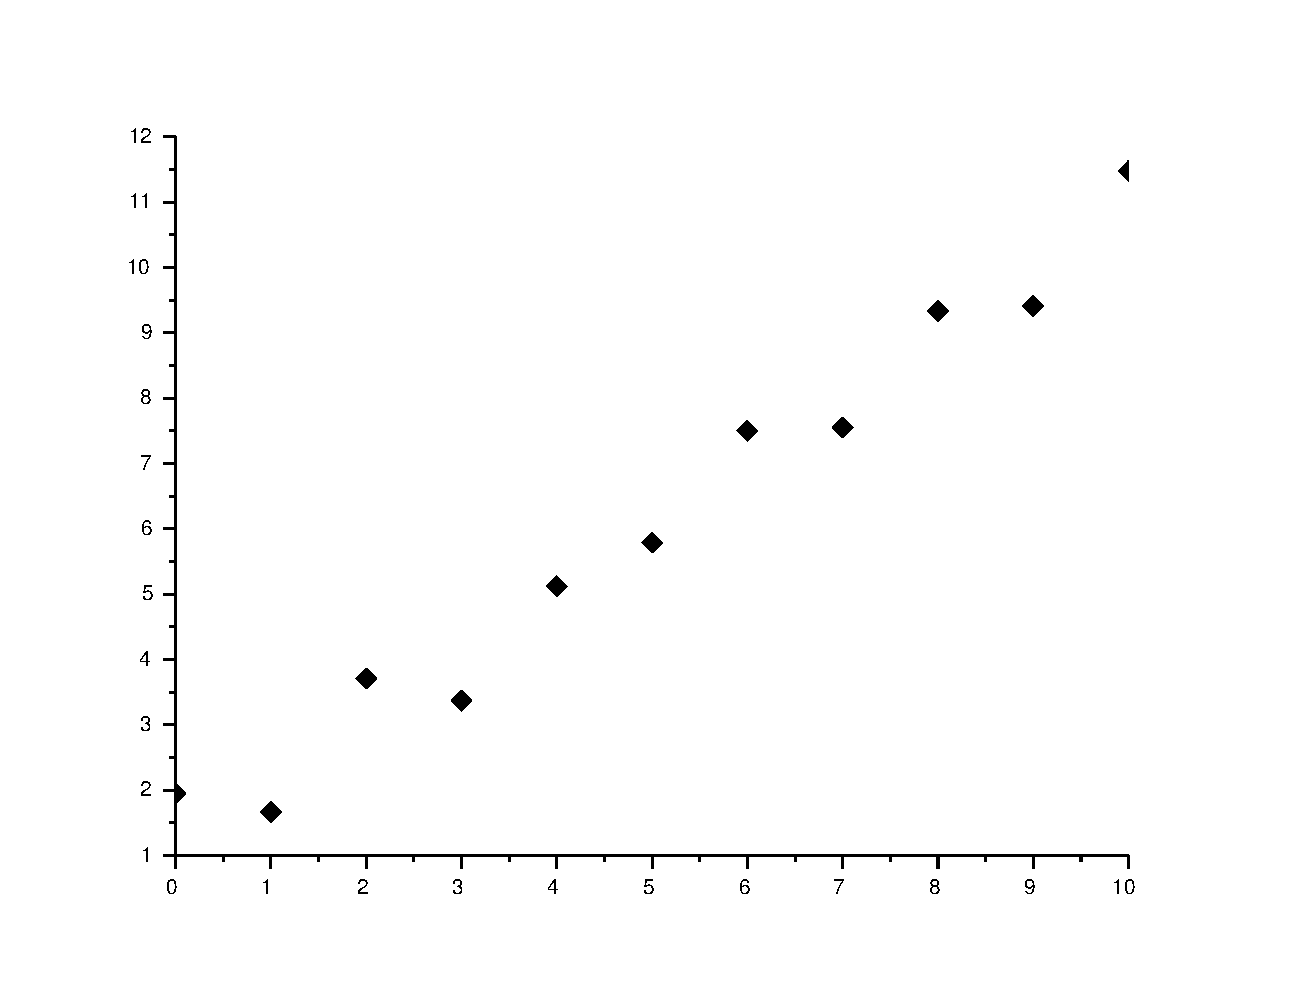
\includegraphics[scale=0.5]{./cap_derivacao/pics/graf_der.eps}
\end{center}

Observe que as derivadas calculadas por diferenças finitas oscilam entre um valor pequeno e um grande em cada intervalo e além disso, a fórmula progressiva difere da regressiva significantemente. Por exemplo, por diferenças regressivas $f'(7)\approx \frac{(7,55 -  7,50)}{1}=0,05$ e por diferenças progressivas $f'(7)\approx \frac{(9,33 -  7,55)}{1}=1,78$. A melhor forma de calcular a derivada aqui é fazer um ajuste de curva. A reta que melhor ajusta os dados da tabela é $y=f(x)=1,2522727+0,9655455x$. Usando esse ajuste, temos $f'(7)\approx 0,9655455$.

\subsection*{Exercícios resolvidos}

\construirExeresol

\subsection*{Exercícios}

\construirExer


\section{Exercícios finais}

\emconstrucao

%Este trabalho está licenciado sob a Licença Creative Commons Atribuição-CompartilhaIgual 3.0 Não Adaptada. Para ver uma cópia desta licença, visite https://creativecommons.org/licenses/by-sa/3.0/ ou envie uma carta para Creative Commons, PO Box 1866, Mountain View, CA 94042, USA.

%\documentclass[main.tex]{subfiles}
%\begin{document}

\chapter{Integração numérica}\index{integração} \label{cap:integracao}

Neste capítulo discutiremos técnicas numéricas para aproximar \emph{integrais}\index{integral} definidas de funções reais. Mais precisamente, considere o problema de calcular (ou aproximar) a integral de $f(x)$ no intervalo $[a,b]$, ou seja,
\begin{equation}
 I = \int_a^b f(x) \;dx.
\end{equation}

\begin{figure}
  \centering
  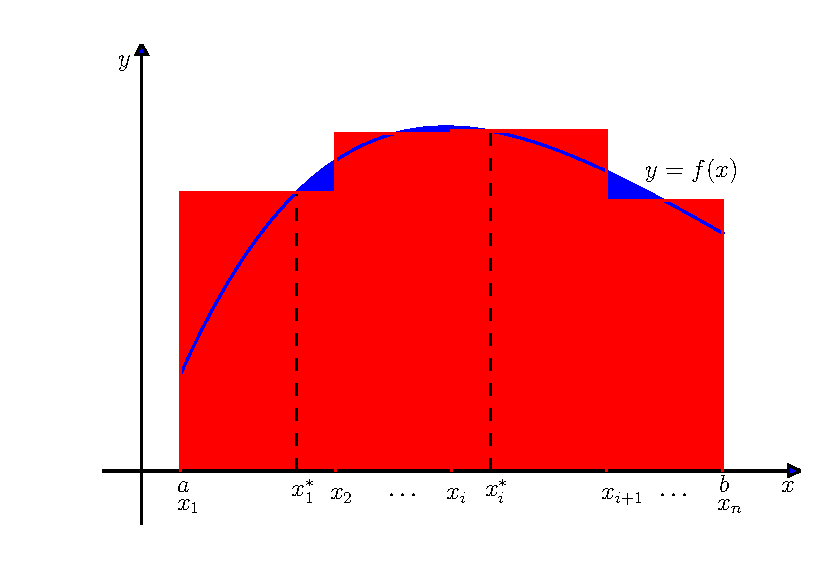
\includegraphics[scale=1.0]{./cap_integracao/pics/Somas_de_Riemann/Somas_de_Riemann}
  \caption{Aproximação da integral definida de uma função.}
  \label{fig:Somas_de_Riemann}
\end{figure}

Geometricamente, $I$ corresponde a área\footnote{área líquida} entre o gráfico de $f(x)$ e o eixo das abscissas (eixo $x$). Uma maneira de aproximar $I$ consiste em subdividir o intervalo $[a,b]$ em $n-1$ subintervalos a partir de um conjunto ordenado de pontos $a=x_1<x_2<...<x_n=b$. Então, temos:
\begin{equation}\label{eq:integral_particionada}
  \begin{split}
    I &= \int_a^b f(x)\,dx\\
    &= \int_{x_1}^{x_2}f(x)\,dx + \int_{x_2}^{x_3}f(x)\,dx + \cdots + \int_{x_{n-1}}^{x_{n}}f(x)\,dx\\
    &= \sum_{i=1}^{n-1}\int_{x_i}^{x_{i+1}}f(x)\,dx
  \end{split}
\end{equation}
Agora, supondo que o tamanho de cada cada subintervalo $h_i = x_{i+1}-x_{i}$ é suficientemente pequeno, podemos aproximar $f(x)$ no intervalo $(x_i, x_{i+1})$ por $f(x_i^*)$ escolhendo arbitrariamente $x_i^{*}\in [x_i, x_{i+1}]$. Desta forma, temos
\begin{equation}
  \int_{x_i}^{x_{i+1}}f(x)\,dx \approx f(x_i^*)h_i.
\end{equation}
Isto é equivalente a aproximar a área entre o gráfico de $f(x)$ e o eixo $x$ restrito ao intervalo $[x_i, x_{i+1}]$ pelo retângulo de base $h_i$ e altura $f(x_i^*)$ (veja Figura~\ref{fig:Somas_de_Riemann}). Consequentemente, de \eqref{eq:integral_particionada} temos
\begin{eqnarray}
  I &=& \int_{a}^{b}f(x)\,dx = \sum_{i=1}^{n-1}\int_{x_i}^{x_{i+1}}f(x)\,dx\\
  I &\approx& \sum_{i=1}^{n-1} f(x_i^*)h_i.
\end{eqnarray}

\begin{figure}
  \centering
  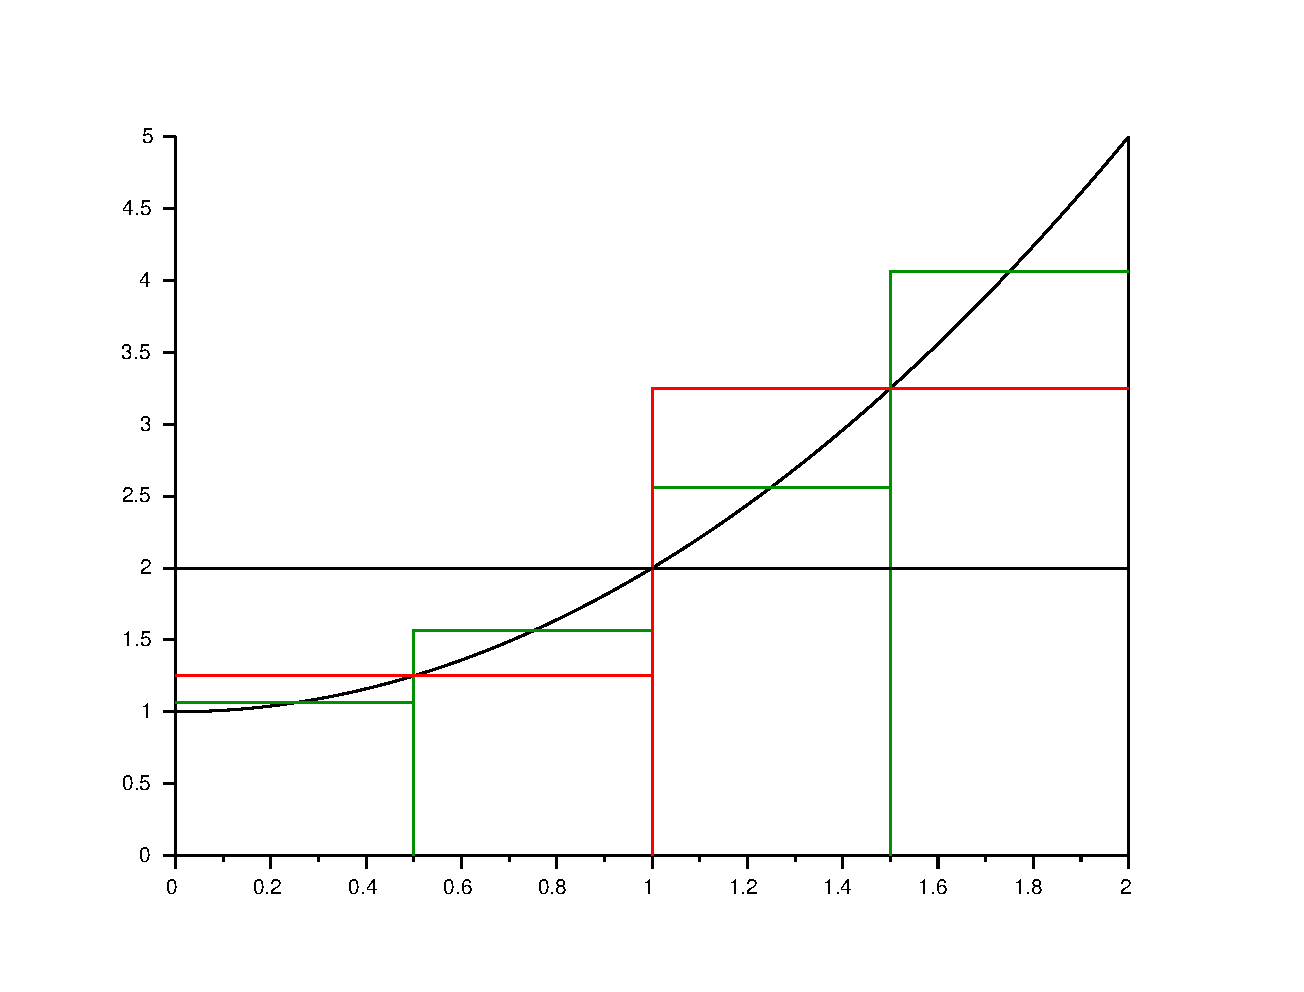
\includegraphics[scale=0.7]{./cap_integracao/pics/int_1/int_1}
  \caption{Aproximação por retângulos.}
  \label{fig:int_101}
\end{figure}

\begin{ex}
A Figura~\ref{fig:int_101} mostra um exemplo quando $f(x)=x^2+1$, $0\leq x\leq 2$. Temos a aproximação por um retângulo com base $h_1=2$, depois com dois retângulos de base $h_2=1$ e, finalmente com quatro retângulos de bases $h_3=0,5$. Os valores aproximados para a integral são dados na seguinte tabela:
\begin{center}
  \begin{tabular}{|c|c|}\hline
    & $\displaystyle \int_0^2(x^2+1)\,dx$ \\ \hline
    $h_1=2$ & $h_1f(1)=4$ \\
    $h_2=1$ & $h_2f(0,5)+h_2f(1,5)=4,5$ \\
    $h_3=0,5$ & $4,625$ \\
    $h_4=0,25$ & $4,65625$ \\\hline
  \end{tabular}
\end{center}
Observe que:
\begin{equation}
  \int_0^2(x^2+1)\,dx = \left[\frac{x^3}{3}+x\right]_0^2 = \frac{8}{3}+2=4,6666667.
\end{equation}
\end{ex}


Uma tal aproximação de uma integral definida
\begin{equation}
  \int_a^b f(x)\,dx \approx \sum_{i} f(x_i)w_i,
\end{equation}
é chamada de quadratura numérica, onde os números $x_i$ denotam seu $i$-ésimo ponto e $w_i$ seu $i$-ésimo peso. Nas próximas seções, mostraremos como obter diferentes quadraturas numéricas e discutiremos sobre suas características.

% Em cada intervalo $[x_i, x_{i+1}]$, a integral será aproximada por $\Delta S_i$ e a integral será aproximada por
% \begin{equation}
%  I \approx S = \sum_{i=1}^{n-1} \Delta S_i.
% \end{equation}
% O tamanho de cada intervalo é dado por $h_i=x_{i+1}-x_i$. No caso uniforme, todos os intervalos possuem o mesmo tamanho $h=h_i=(b-a)/(n-1)$.

% Nas próximas seções apresentaremos formas diferentes de aproximar $\Delta S_i$ iniciando com o caso mais simples que é um retângulo. Cada uma das regras obtidas também é chamada de quadratura.

%%%%%%%%%%%%%%%%%%%%
% python
%%%%%%%%%%%%%%%%%%%%
\ifispython
Nos códigos \verb+Python+ apresentados ao longo deste capítulo, assumiremos o seguinte:
\begin{verbatim}
>>> import numpy as np
\end{verbatim}
\fi
%%%%%%%%%%%%%%%%%%%%

\section{Somas de Riemann}
O método mais simples de aproximar
\begin{equation}
 I = \int_a^b f(x) \;dx.
\end{equation}
com apenas um intervalo, é aproximar $f(x)$ por um polinômio constante no intervalo $[a,b]$, ou seja, $f(x)=c$. Se aproximarmos $f(x)$ pelo ponto à esquerda do intervalo temos que $f(x)\approx f(a)$ e
\begin{eqnarray}
 I &=& \int_a^b f(x) \;dx\\
   &\approx& \int_a^b f(a) \;dx \\
   &=& f(a) \int_a^b\,dx\\
   &=& f(a) (b-a)
\end{eqnarray}
Esta é a regra de quadratura local para $1$ intervalo.

Quando subdividimos $[a,b]$ em $n$ intervalos com tamanho $h=(b-a)/n$ nos pontos $x_i=a+(i-1)h$ , em cada intervalo $i$ aproximamos a área por
\begin{equation}
  \Delta S_i \approx f(x_i)h
\end{equation}
tal que a área total será aproximada pelas \emph{somas de Riemann à esquerda}
\begin{equation}
S =\sum_{i=1}^{n} \Delta S_i = \sum_{i=1}^{n} f(x_i) h
\end{equation}
Podemos obter uma fórmula similar se usarmos os pontos à direita do intervalo, ou seja, as \emph{somas de Riemann à direita}
\begin{equation}
S = \sum_{i=1}^{n} f(x_{i+1}) h
\end{equation}

Uma terceira opção é utilizar o ponto médio do intervalo $[x_i,x_{i+1}]$ o qual fornece a \emph{regra do ponto médio}
\begin{equation}\label{eq:regra_do_ponto_medio}
S = \sum_{i=1}^{n} f(\xi_i ) h, \qquad \xi_i=\frac{x_i+x_{i+1}}{2}.
\end{equation}

\begin{ex}
  A integral de $f(x) = e^{-x}\sen(x)$ no intervalo $[0,1, 0,2]$ é
  \begin{equation}
    \int_{0}^{1} f(x)\,dx \approx 2,45837\E-1.
  \end{equation}
Usando somas de Riemann à esquerda com $10$ intervalos, obtemos
\begin{equation}
  \int_0^1 f(x)\,dx \approx \sum_{i=1}^{10} f(x_{i})h = 2,29433\times 10^{-1}.
\end{equation}
onde $h=0,1$ e $x_i=(i-1)h$. Analogamente, usando somas de Riemann à direita, obtemos
\begin{equation}
  \int_0^1 f(x)\,dx \approx \sum_{i=1}^{10} f(x_{i+1})h = 2,60389\times 10^{-1}.
\end{equation}
E, usando a regra do ponto médio, temos
\begin{equation}
  \int_0^1 f(x)\,dx \approx \sum_{i=1}^{10} f\left(\frac{x_i+x_{i+1}}{2}\right)h = 2,46300\times 10^{-1}.
\end{equation}

%%%%%%%%%%%%%%%%%%%%
% scilab
%%%%%%%%%%%%%%%%%%%%
\ifisscilab
\construirScilab
\fi
%%%%%%%%%%%%%%%%%%%%
%%%%%%%%%%%%%%%%%%%%
% octave
%%%%%%%%%%%%%%%%%%%%
\ifisoctave
No \verb+GNU Octave+, podemos computar as somas de Riemann à esquerda da seguinte forma:
\begin{verbatim}
f = @(x) exp(-x)*sin(x);
a=0;
b=1;
n=10;
h=(b-a)/n;
x=0:h:1;
s=0;
for i=1:n
  s += f(x(i))*h;
endfor
printf("%1.5e\n",s)
\end{verbatim}
\fi
%%%%%%%%%%%%%%%%%%%%
%%%%%%%%%%%%%%%%%%%%
% python
%%%%%%%%%%%%%%%%%%%%
\ifispython
Pode-se, no \verb+Python+, implementar as somas de Riemman da seguinte forma
\begin{verbatim}
f = lambda x: np.exp(-x)*np.sin(x)

a = 0
b = 1
n = 10
h = (b-a)/n
x = np.linspace(a,b,n+1)

S_esq = 0
S_dir = 0
S_med = 0

print("Soma de Riemman de {} a {} com {} intervalos:\n".format(a, b, n))

for i in range(n):
    S_esq += f(x[i])*h
print("A esquerda: {:.5e}".format(S_esq))

for i in range(n):
    S_dir += f(x[i+1])*h
print("A direita: {:.5e}".format(S_dir))

for i in range(n):
    S_med += f(((x[i]) + (x[i+1]))/2)*h
print("Pelo ponto medio: {:.5e}".format(S_med))
\end{verbatim}
%\construirPython
\fi
%%%%%%%%%%%%%%%%%%%%
\end{ex}

\subsection*{Exercícios resolvidos}

\construirExeresol

\subsection*{Exercícios}

\construirExer


\section{Regras de Newton-Cotes}\index{integração numérica!regras de Newton-Cotes}


O método básico para encontrar as regras de integração consiste em aproximar a integral de $f$ por uma combinação linear de $n$ valores de $y_i := f(x_i)$, ou seja,
\begin{equation}
I = \int_a^b f(x) \;dx \approx \sum_{i=1}^nA_iy_i.
\end{equation}

% Quanto maior o número de pontos $n$, melhor será a regra de quadratura.

Podemos obter os coeficientes $A_i$ aproximando a função $f$ pelo polinômio de Lagrange $p_{n-1}$ que interpola $\{(x_i,y_i)\}_{i=1}^n$, tal que,
\begin{eqnarray}
  f(x) &=& p_n(x)+E^n_{LAG}(x) \\
       &=& \sum_{i=1}^n y_iL_i(x)+E^n_{LAG}(x)
\end{eqnarray}
onde o erro na interpolação de Lagrange é
\begin{equation}
   E^n_{LAG}(x)=\frac{f^{(n)}(\xi(x))}{n!}\prod_{i=1}^n(x-x_i).
\end{equation}

Substituindo na integral, obtemos:
\begin{equation}
  \int_a^bf(x)\,dx = \sum_{i=1}^n\left[y_i\int_a^bL_i(x)\,dx\right] +  \int_a^b E^n_{LAG}(x) \;dx.
%   \int_a^bf(x)dx &=& \sum_{i=1}^n\left[f(x_i)\int_a^bL_i(x)dx\right] +  \frac{1}{(n+1)!}\int_a^b\prod_{i=1}^n(x-x_i)f^{(n+1)}(\xi)dx.
\end{equation}

A fórmula de quadratura é então
\begin{equation}
  \int_a^bf(x)\,dx\approx\sum_{i=1}^nA_iy_i,
\end{equation}
onde
\begin{equation}
  A_i=\int_a^b L_i(x)\;dx.
\end{equation}

% Considere o problema de calcular a área entre uma função positiva, o eixo $x$ e as retas $x=a$ e $x=b$. O valor exato dessa área é calculada fazendo uma aproximação por retângulos com bases iguais e depois tomando o limite quando o número de retângulos tende ao infinito:
% \begin{equation}
% A=\lim_{n\to\infty}\sum_{i=1}^nf(x_i)h_n,
% \end{equation}
% onde $h_n=\frac{b-a}{n}$ é o tamanho da base dos retângulo e $f(x_i)$, $1\leq i\leq n$, $a+(i-1)h\leq x_i\leq a+ih$, é a altura dos retângulos. Essa definição é generalizada para cálculo de integrais em um intervalo $[a,b]$:
% \begin{equation}
% \int_a^bf(x)dx=\lim_{n\to\infty}\sum_{i=1}^nf(x_i)h_n.
% \end{equation}



% \section{Regras de Newton-Cotes}\index{integração numérica!regras de Newton-Cotes}

% A integral de uma função em um intervalo $[a, b]$, também chamada de quadratura numérica, é aproximada pela soma:
% \begin{equation}
%   \int_a^b f(x)\,dx \approx \sum_{i=1}^n a_if(x_i),
% \end{equation}
% onde $x_i$, $1\leq i\leq n$, são pontos distintos do intervalo $[a,b]$. Nesta definição, a integral $\int_0^2(x^2+1)dx$ usando uma aproximação por retângulo usa apenas um ponto, o ponto médio do intervalo ($x_1=1$) e a soma se reduz a uma parcela ($(2-0)f(1)$). A fórmula geral para essa caso, chamado de regra do ponto médio é:
% \begin{equation}\label{ponto_medio_1}
% \int_a^bf(x)dx\approx (b-a)f\left(\frac{a+b}{2}\right):=hf(x_1).
% \end{equation}

% \subsection{Erro na regra do ponto médio}\index{integração numérica!regra do ponto médio}
% A regra do ponto médio \eqref{ponto_medio_1} pode ser deduzida mais formalmente usando a expansão de Taylor
% \begin{equation}
% f(x)=f(x_1)+f'(x_1)(x-x_1)+\frac{f''(\xi(x))}{2}(x-x_1)^2
% \end{equation}
% que leva a integral
% \begin{equation}
% \int_a^b f(x)dx=\int_a^b f(x_1) dx+f'(x_1)\int_a^b(x-x_1)dx +\int_a^b\frac{f''(\xi(x))}{2}(x-x_1)^2dx.
% \end{equation}
% Usando o teorema do valor médio para integrais e que $h=b-a$ e $x_1=(a+b)/2$, temos:
% \begin{eqnarray}
% \int_a^b f(x)dx &=& h f(x_1) + f'(x_1)\int_a^b(x-x_1)dx+f''(\eta)\int_a^b\frac{1}{2}(x-x_1)^2dx\\
%  &=& h f(x_1) +f'(x_1)\left[\frac{(x-x_1)^2}{2}\right]_a^b+f''(\eta)\left[\frac{1}{6}(x-x_1)^3\right]_a^b\\
%  &=& h f(x_1) +f'(x_1)\left[\frac{(b-x_1)^2}{2}-\frac{(a-x_1)^2}{2}\right]\\
%  &+& f''(\eta)\left[\frac{1}{6}(b-x_1)^3-\frac{1}{6}(a-x_1)^3\right]\\
%  &=& h f(x_1) +\frac{h^3f''(\eta)}{3}.
% \end{eqnarray}
% para $a\leq \eta\leq b$, onde o erro local é $\mathcal{O}(h^3)$.


% \begin{ex}
% Use a regra do ponto médio para aproximar a integral
% \begin{equation}
% \int_0^1e^{-x^2}dx.
% \end{equation}
% Depois divida a integral em duas
% \begin{equation}
% \int_0^{1/2}e^{-x^2}dx+\int_{1/2}^{1}e^{-x^2}dx.
% \end{equation}
% e aplique a regra do ponto médio em cada uma delas. Finalmente, repita o processo dividindo em quatro integrais.

% Usando o intervalo $[0,1]$, temos $h=1$ e $x_1=1/2$. A regra do ponto médio resulta em
% \begin{equation}
% \int_0^1e^{-x^2}dx\approx 1\cdot e^{-1/4}=0,7788008
% \end{equation}
% Usando dois intervalos, $[0,1/2]$ e $[1/2,1]$ e usando a regra do ponto médio em cada um dos intervalos, temos:
% \begin{equation}
% \int_0^1e^{-x^2}dx\approx 0,5\cdot e^{-1/16}+0,5\cdot e^{-9/16})=0,4697065+0,2848914=0,7545979
% \end{equation}
% Agora, usando quatro intervalos, temos
% \begin{equation}
% \int_0^1e^{-x^2}dx\approx 0,25\cdot e^{-1/64}+0,25\cdot e^{-9/64}+0,25\cdot e^{-25/64}+0,25\cdot e^{-49/64}=0,7487471
% \end{equation}
% Observe que o valor da integral é
% \begin{equation}
% \int_0^1e^{-x^2}dx=0,7468241330.
% \end{equation}
% \end{ex}

\subsection{Regra do ponto médio}

A regra do ponto médio \eqref{eq:regra_do_ponto_medio} é uma quadratura de Newton-Cotes de um ponto. Neste caso, temos $x_1 = (a+b)/2$ e o polinômio interpolador é o polinômio de grau zero
\begin{equation}
  p(x) = f(x_1)L_1(x) = f(x_1),
\end{equation}
uma vez que $L_1(x)\equiv 1$. Então, temos
\begin{equation}
  \begin{split}
    \int_a^b f(x)\,dx &\approx \int_a^b p(x)\,dx\\
    &= \int_a^b f(x_1)\,dx\\
    &= f(x_1)\int_a^b\,dx\\
    &= hf\left(\frac{a+b}{2}\right),
  \end{split}
\end{equation}
onde $h=b-a$.

\begin{ex}
  Usando a regra do ponto médio, temos
  \begin{equation}
    \begin{split}
    \int_{0,1}^{0,3} e^{-x}\sen(x)\,dx &\approx (a-b) f\left(\frac{a+b}{2}\right) \\
    &= 0,2e^{-0,2}\sen(0,2) = 3,25313\times 10^{-2}.
    \end{split}
  \end{equation}

%%%%%%%%%%%%%%%%%%%%
% scilab
%%%%%%%%%%%%%%%%%%%%
\ifisscilab
\construirScilab
\fi
%%%%%%%%%%%%%%%%%%%%
%%%%%%%%%%%%%%%%%%%%
% octave
%%%%%%%%%%%%%%%%%%%%
\ifisoctave
No \verb+GNU Octave+, computamos:
\begin{verbatim}
f = @(x) exp(-x)*sin(x);
a=0.1;
b=0.3;
h=b-a;
I = h*f((a+b)/2)
\end{verbatim}
\fi
%%%%%%%%%%%%%%%%%%%%
%%%%%%%%%%%%%%%%%%%%
% python
%%%%%%%%%%%%%%%%%%%%
\ifispython
No \verb+Python+, computamos:
\begin{verbatim}
f = lambda x: np.exp(-x)*np.sin(x)

a=0.1
b=0.3
h=b-a

I = h*f((a+b)/2)
\end{verbatim}
%\construirPython
\fi
%%%%%%%%%%%%%%%%%%%%
\end{ex}



\subsection{Regra do trapézio}\index{integração numérica!regra do trapézio}\label{sec:trapezio}

A regra do trapézio consiste em aproximar a função $f(x)$ por um polinômio de grau 1. O nome do método vem do fato que a região entre o eixo $x$ e a reta que liga os pontos sobre o gráfico da função nos extremos do intervalo forma um trapézio.

% \begin{center}
% 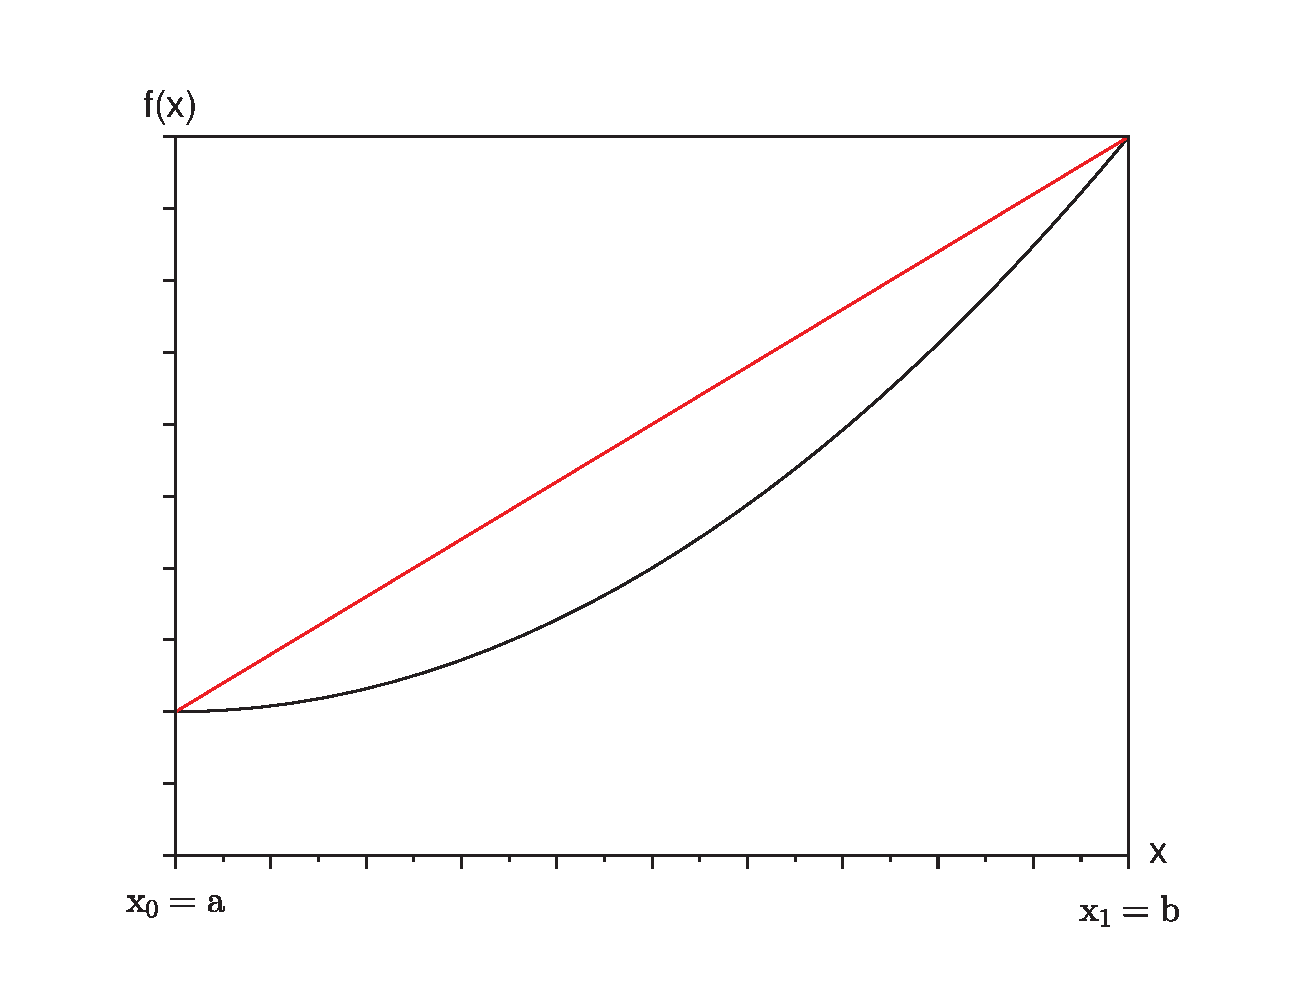
\includegraphics[scale=0.7]{./cap_integracao/pics/int_2/int_2}
% \end{center}

Aqui, utilizamos $x_1:=a$,  $x_2:=b$, $h=x_2-x_1$ e a notação $y_i=f(x_i)$, e obtemos através da interpolação de Lagrange o polinômio
\begin{eqnarray}
p_1(x) &=& y_1 L_1(x)+ y_2 L_2(x)
\end{eqnarray}
Aproximando $f(x)$ por $p_1(x)$ e integrando, obtemos:
\begin{eqnarray}
  \int_a^bf(x)\;dx &\approx& \int_a^bp_1(x)\;dx \\
    &=& \int_a^b y_1L_1(x) + y_2L_2(x)\;dx \\
    &=& y_1 \int_a^b L_1(x)\;dx + y_2 \int_a^b L_2(x)\;dx \\
    &=& A_1 y_1 + A_2 y_2,
\end{eqnarray}
onde
\begin{eqnarray}
  A_1 &=& \int_{x_1}^{x_2}\frac{x-x_2}{x_1-x_2}dx =  \left[\frac{(x-x_2)^2-x_2^2}{2h}\right]_{x_1}^{x_2}\\
      &=& \frac{(x_2-x_1)^2}{2h} = \frac{h^2}{2h} = \frac{1}{2}h.
\end{eqnarray}
Da mesma forma,
\begin{eqnarray}
  A_2 &=& \int_{x_1}^{x_2}\frac{(x-x_1)}{(x_2-x_1)}\,dx = \frac{1}{2}h,
\end{eqnarray}
de onde obtemos a \emph{regra do trapézio} dada por:
\begin{equation}
  \int_a^b f(x)\;dx \approx \left(\frac{1}{2}f(a) + \frac{1}{2}f(b)\right)h.
\end{equation}


\subsubsection{Erro na regra do trapézio}
O \textit{erro na regra do trapézio} pode ser obtido integrando o erro da interpolação de Lagrange,
\begin{eqnarray}
   E_{TRAP} = \int_a^b E^2_{LAG}(x) \;dx= \int_a^b \frac{f''(\xi(x))}{2!}(x-x_1)(x-x_2) \;dx.
\end{eqnarray}
Pelo teorema do valor médio, existe $a\leq \eta\leq b$ tal que
\begin{eqnarray}
    E_{TRAP} = \frac{f''(\eta)}{2!}\int_a^b (x-x_1)(x-x_2) \;dx,
\end{eqnarray}
portanto
\begin{eqnarray}
     E_{TRAP}
  &=& \frac{f''(\eta)}{2}\left[\frac{x^3}{3}-\frac{x^2}{2}(x_2+x_1)+x_1x_2x\right]_{x_1}^{x_2}\\
  &=& \frac{f''(\eta)}{2}\left(\frac{x_2^3}{3}-\frac{x_2^2}{2}(x_2+x_1)+x_1x_2x_2-\frac{x_1^3}{3}+\frac{x_1^2}{2}(x_2+x_1)-x_1x_2x_1\right)\\
  &=& \frac{f''(\eta)}{2}\frac{2x_2^3-3x_2^2(x_2+x_1)+6x_2^2x_1-2x_1^3+3x_1^2(x_2+x_1)-6x_2x_1^2}{6}\\
  &=& \frac{f''(\eta)}{12}\left(x_1^3-3x_1^2x_2+3x_2^2x_1-x_2^3\right)
   =  \frac{f''(\eta)}{12}(x_1-x_2)^3\\
  &=& -\frac{f''(\eta)}{12}h^3.
\end{eqnarray}

Assim, o erro na regra do trapézio é
\begin{equation}
E_{TRAP}  = -\frac{f''(\eta)}{12}h^3 = \mathcal{O}(h^3).
\end{equation}

\begin{ex}
Use a regra do trapézio para aproximar a integral
\begin{equation}
\int_0^1e^{-x^2}\;dx.
\end{equation}
Depois divida a integral em duas
\begin{equation}
\int_0^{1/2}e^{-x^2}\;dx+\int_{1/2}^{1}e^{-x^2}\;dx.
\end{equation}
e aplique a regra do trapézio em cada uma delas. Finalmente, repita o processo dividindo em quatro integrais.
\end{ex}
Usando o intervalo $[0,1]$, temos $h=1$, $x_0=0$ e $x_1=1$. A regra do trapézio resulta em
\begin{equation}
\int_0^1e^{-x^2}\;dx\approx \frac{1}{2}(e^{0}+e^{-1})=0,6839397.
\end{equation}
Usando dois intervalos, $[0,1/2]$ e $[1/2,1]$ e usando a regra do trapézio em cada um dos intervalos, temos:
\begin{eqnarray}
\int_0^1e^{-x^2}\;dx &\approx& \frac{0,5}{2}\left(e^{0}+e^{-1/4}\right) + \frac{0,5}{2}\left(e^{-1/4}+e^{-1}\right) \\
&=& 0,4447002+0,2866701 =0,7313703.
\end{eqnarray}
Agora, usando quatro intervalos, temos
\begin{eqnarray}
\int_0^1e^{-x^2}\;dx &\approx& \frac{0,25}{2}\left(e^{0}+e^{-1/16}\right) + \frac{0,25}{2}\left(e^{-1/16}+e^{-1/4}\right) \\
&+& \frac{0,25}{2}\left(e^{-1/4}+e^{-9/16}\right)+\frac{0,25}{2}\left(e^{-9/16}+e^{-1}\right) \\
&=& 0,7429841.
\end{eqnarray}



\subsection{Regra de Simpson}\index{integração numérica!regra de Simpson}
Na regra de Simpson aproximamos $f$ por um polinômio de grau $2$, portanto precisamos de três pontos do intervalo $[a,b]$. Utilizando, por definição,
\begin{equation}
x_1:=a,\qquad x_2:=\frac{a+b}{2}\qquad \text{e}\qquad x_3:=b
\end{equation}
com $h=\frac{x_3-x_1}{2}$, isto é, a distância entre dois pontos consecutivos, podemos obter o polinômio de Lagrange
\begin{equation}
    p_2(x) = y_1L_1(x) + y_2L_2(x)  + y_3L_3(x),
\end{equation}
onde $y_i=f(x_i)$, $i=1,2,3$.

Aproximando $f(x)$ por $p_2(x)$ e integrando temos
\begin{eqnarray}
\int_a^bf(x)\;dx &\approx&\int_a^b p_2(x) \;dx \\
               &=&\int_a^b y_1L_1(x) + y_2L_2(x)  + y_3L_3(x) \;dx \\
               &=&y_1 A_1 + y_2A_2  + y_3A_3
\end{eqnarray}
onde
\begin{eqnarray}
  A_i = \int_a^b L_i(x) \;dx
\end{eqnarray}
Calculando essas integrais obtemos \emph{a regra de Simpson}:
\begin{equation}
\int_a^bf(x)\;dx=\left(\frac{1}{3}f(a)+\frac{4}{3}f\left(\frac{a+b}{2}\right)+\frac{1}{3}f(b)\right)h.
\end{equation}

\begin{ex}
Obtenha os coeficientes $A_i$ do método de Simpson  integrando os polinômios de Lagrange $L_i(x)$.

Fazendo uma translação para a origem (subtraindo $x_1$ de $x_2$ e $x_3$)
\begin{eqnarray}
   A_1 &=& \int_{x_1}^{x_3} \frac{(x-x_2)(x-x_3)}{(x_1-x_2)(x_1-x_3)}\;dx \\
       &=& \int_0^{2h} \frac{(x-h)(x-2h)}{(0-h)(0-2h)}\;dx
        =  \frac{1}{2h^2} \int_0^{2h} (x-h)(x-2h)\;dx \\
        &=& \frac{1}{2h^2} \int_0^{2h} \left(x^2 -3hx+2h^2\right)dx
        =  \frac{1}{2h^2} \left.\left(\frac{1}{3}x^3 -\frac{3}{2}hx^2+2h^2x\right)\right|_0^h \\
       &=& \frac{1}{2h^2} \left(\frac{1}{3}h^3 -\frac{3}{2}h^3+2h^3\right)
      = \frac{h}{3}.
\end{eqnarray}
Apesar de longa, é apenas a integral de um polinômio de grau 2. De forma semelhante podemos obter
\begin{equation}
A_2 = \frac{4}{3}h, \;\;\; A_3 = \frac{1}{3}h
\end{equation}
Assim, lembrando que $h=\frac{b-a}{2}$, temos:
\begin{equation}
 \int_a^b f(x)dx \approx \frac{b-a}{6}\left[f(a)+4f\left(\frac{a+b}{2}\right)+f(b)\right].
 \end{equation}

\end{ex}



\subsubsection{Erro na regra de Simpson}\index{integração numérica!regra de Simpson}
Se usarmos a mesma metodologia da regra dos trapézios, teremos
\begin{equation}
\int_a^bf(x)\;dx=\int_a^bp_2(x)\;dx+\int_a^b\frac{(x-x_1)(x-x_2)(x-x_3)}{6}f'''(\xi(x))\;dx
\end{equation}
e obteremos o fórmula de Simpson com um erro de quarta ordem. O fato é que a regra de Simpson tem ordem cinco e, para isso, usaremos uma abordagem alternativa.

Considere o polinômio de Taylor em $x_2$,
\begin{equation}
f(x)=f(x_2)+f'(x_2)(x-x_2)+\frac{f''(x_2)}{2}(x-x_2)^2+\frac{f'''(x_2)}{6}(x-x_2)^3+\frac{f^{(4)}(\xi(x))}{24}(x-x_2)^4,
\end{equation}
onde $x_1\leq\xi(x)\leq x_3$ e integre no intervalo $[a,b]=[x_1,x_3]$:
\begin{equation}
  \begin{split}
    \int_a^bf(x)\;dx&= \left[f(x_2)(x-x_2)+f'(x_2)\frac{(x-x_2)^2}{2} + \frac{f''(x_2)}{6}(x-x_2)^3\right. \\
      &\left. + \frac{f'''(x_2)}{24}(x-x_2)^4\right]_{x_1}^{x_3}\\
      &+ \frac{1}{24}\int_{x_1}^{x_3}f^{(4)}(\xi(x))(x-x_2)^4\;dx,
  \end{split}
\end{equation}
Pelo teorema do valor médio, existe $x_1\leq\eta\leq x_3$ tal que
\begin{equation}
  \begin{split}
    \int_a^bf(x)\;dx&= \left[f(x_2)(x-x_2)+f'(x_2)\frac{(x-x_2)^2}{2}+\frac{f''(x_2)}{6}(x-x_2)^3\right.\\
    &+\left.\frac{f'''(x_2)}{24}(x-x_2)^4\right]_{x_1}^{x_3}\\
    &+ \frac{f^{(4)}(\eta)}{24}\int_{x_1}^{x_3}(x-x_2)^4\;dx\\
    &= \left[f(x_2)(x-x_2)+f'(x_2)\frac{(x-x_2)^2}{2}+\frac{f''(x_2)}{6}(x-x_2)^3\right.\\
    &+\left.\frac{f'''(x_2)}{24}(x-x_2)^4\right]_{x_1}^{x_3}\\
    &+ \frac{f^{(4)}(\eta)}{120}\left[(x-x_2)^5\right]_{x_1}^{x_3}.
  \end{split}
\end{equation}
Usando o fato que
\begin{equation}
(x_3-x_2)^3-(x_1-x_2)^3=2h^3,
\end{equation}
\begin{equation}
(x_3-x_2)^4-(x_1-x_2)^4=0
\end{equation}
e
\begin{equation}
(x_3-x_2)^5-(x_1-x_2)^5=2h^5,
\end{equation}
temos
\begin{equation}
\int_a^bf(x)\;dx=2hf(x_2)+\frac{h^3}{3}f''(x_2)+\frac{h^5f^{(4)}(\eta)}{60}.
\end{equation}
Usando a fórmula de diferenças finitas centrais para a derivada segunda:
\begin{equation}
f''(x_2)=\frac{f(x_1)-2f(x_2)+f(x_3)}{h^2}-\frac{h^2}{12}f^{(4)}(\eta_2),
\end{equation}
$x_1\leq \eta_2\leq x_3$, temos
\begin{eqnarray}
\int_a^bf(x)\;dx&=&2hf(x_2)+\frac{h^3}{3}\left(\frac{f(x_1)-2f(x_2)+f(x_3)}{h^2}-\frac{h^2}{12}f^{(4)}(\eta_2)\right)\\
&+&\frac{h^5f^{(4)}(\eta)}{60}\\
&=&\frac{h}{3}\left(f(x_1)+4f(x_2)+f(x_3)\right)-\frac{h^5}{12}\left(\frac{1}{3}f^{(4)}(\eta_2)-\frac{1}{5}f^{(4)}(\eta)\right).
\end{eqnarray}
Pode-se mostrar que é possível escolher $\eta_3$ que substitua $\eta$ e $\eta_2$ com a seguinte estimativa
\begin{equation}
\int_a^bf(x)\;dx=\frac{h}{3}\left(f(x_1)+4f(x_2)+f(x_3)\right)-\frac{h^5}{90}f^{(4)}(\eta_3).
\end{equation}

\begin{ex}
Use a regra de Simpson para aproximar a integral
\begin{equation}
\int_0^1e^{-x^2}\;dx.
\end{equation}
Depois divida a integral em duas
\begin{equation}
\int_0^{1/2}e^{-x^2}\;dx+\int_{1/2}^{1}e^{-x^2}\;dx.
\end{equation}
e aplique a regra de Simpson em cada uma delas.
\end{ex}
Usando o intervalo $[0,1]$, temos $h=1/2$, $x_0=0$, $x_1=1/2$ e $x_2=1$. A regra de Simpson resulta em
\begin{equation}
\int_0^1e^{-x^2}\;dx\approx \frac{0,5}{3}(e^{0}+4e^{-1/4}+e^{-1})=0,7471804.
\end{equation}
Usando dois intervalos, $[0,1/2]$ e $[1/2,1]$ e usando a regra de Simpson em cada um dos intervalos, temos:
\begin{equation}
\int_0^1e^{-x^2}\;dx\approx \frac{0,25}{3}(e^{0}+4e^{-1/16}+e^{-1/4})+\frac{0,25}{3}(e^{-1/4}+4e^{-9/16}+e^{-1})=0,7468554.
\end{equation}

\subsection*{Exercícios resolvidos}

\construirExeresol

\subsection*{Exercícios}

\begin{exer}Calcule numericamente as seguintes integrais:
  \begin{eqnarray}
    \text{a)}~\int_0^1e^{-x}\,dx & \text{b)}~\int_0^1x^2\,dx\\
    \text{c)}~\int_0^1x^3\,dx & \text{d)}~\int_0^1xe^{-x^2}\,dx\\
    \text{e)}~\int_0^1\frac{1}{x^2+1}\,dx &\text{e)}~\int_0^1\frac{x}{x^2+1}\;dx
  \end{eqnarray}
usando os métodos simples do ponto médio, Trapézio e Simpson. Calcule, também, o valor analítico destas integrais e o erro nas aproximações dadas pelas quadraturas numéricas.
\end{exer}
% \begin{resp}
%
%  \begin{center}
% \begin{tabular}{|c|c|c|c|c|}
% \hline
%   & exato & Ponto médio & Trapézio & Simpson \\
% \hline
%  & & & &\\[-.3cm]
% $\int_0^1e^{-x}dx$ &$1-e^{-1}\approx 0.6321206$& $ e^{-1/2}\approx 0.6065307$&$\frac{1+e^{-1}}{2}\approx 0.6839397$ &$\frac{1+4e^{-1/2}+e^{-1}}{6}\approx 0.6323337$\\[.2cm]
% \hline
%  & & & &\\[-.3cm]
% $\int_0^1x^2dx $ & $1/3\approx 0.3333333$& 0.25 & 0.5 & 0.3333333\\[.2cm]

% \hline
%  & & & &\\[-.3cm]
% $\int_0^1x^3dx $ & $1/4=0.25$ & 0.125 & 0.5 & 0.25\\[.2cm]
% \hline
%  & & & &\\[-.3cm]
% $\int_0^1xe^{-x^2}dx$  &$\frac{1}{2}\left(1-e^{-1}\right)\approx 0.3160603$ & 0.3894004  &  0.1839397 &   0.3209135  \\[.2cm]
% \hline
%  & & & &\\[-.3cm]
% $\int_0^1\frac{1}{x^2+1}dx$  & $\tan^{-1}(1)\approx 0.7853982$ &  0.8  &  0.75 &   0.7833333
%  \\[.2cm]
% \hline
%  & & & &\\[-.3cm]
% $\int_0^1\frac{x}{x^2+1}dx$  &$\frac{1}{2}\ln(2)\approx  0.3465736  $ & 0.4 & 0.25 & 0.35\\[.2cm]
% \hline
%  & & & &\\[-.3cm]
% $\int_0^1\frac{1}{x+1}dx$  & $\ln(2) \approx 0.6931472$ & 0.6666667  &  0.75 &   0.6944444  \\[.2cm]
% \hline
% \end{tabular}
% \end{center}
%
% \end{resp}

\begin{exer}
 Dê a interpretação geométrica dos métodos do ponto médio, trapézio e Simpson. A partir desta construção geométrica, deduza as fórmulas para aproximar
 \begin{equation} \int_a^bf(x)\;dx. \end{equation}
 Verifique que o método de Simpson pode ser entendido como uma média aritmética ponderada entre os métodos de trapézio e ponto médio. Encontre os pesos envolvidos. Explique o que são os métodos compostos.
 \end{exer}
\begin{resp}
\begin{equation}
  I_{Simpson}= \frac{1}{3} I_{Trap}+ \frac{2}{3}I_{PM}
\end{equation}
\end{resp}


\begin{exer}
Calcule numericamente o valor de $\int_2^5e^{4-x^2}\;dx$ usando os métodos compostos do ponto médio, trapézio e Simpson. Obtenha os resultados utilizando, em cada quadratura, o número de pontos indicado.
\begin{center}
\begin{tabular}{|c|c|c|c|c|}
\hline
n   & Ponto médio & Trapézios & Simpson \\
\hline
$3$ &~\hspace{40pt}~& ~\hspace{40pt}~& ~\hspace{40pt}\\
\hline
$5 $ & & & \\
\hline
$7 $ & & &\\
\hline
$9$  & & &\\
\hline
\end{tabular}
\end{center}
\end{exer}
\begin{resp}
    \begin{equation}
    \begin{array}{c|cccc}
        n   & \text{Ponto médio} & \text{Trapézios} & \text{Simpson} \\  \hline
        3 & 0.1056606  &  0.7503919  &  0.5005225  \\  \hline
        5 & 0.1726140 &   0.3964724  &  0.2784992   \\\hline
        7 & 0.1973663 &   0.3062023  &  0.2393551  \\ \hline
        9  &  0.2084204 &   0.2721145  &  0.2306618  \\ \hline
    \end{array}
    \end{equation}
\end{resp}



\section{Obtenção das regras de quadratura}

Na seção anterior, obtivemos as regras de quadraturas pela aproximação do integrando por polinômios interpoladores de Lagrange. Aqui, veremos um outro método para obter regras de quadratura, que torna-se bastante útil para quando temos muitos pontos ou quando o intervalo entre os pontos não é uniforme.

Dados $n$ pontos $[t_1, t_2, \ldots,t_n]$, queremos obter uma aproximação para
\begin{equation}\label{regraint}
  \int _a^b f(t) \;dt \approx w_1f(t_1)+w_2f(t_2)+\ldots +w_nf(t_n)
\end{equation}
que seja exata para polinômios\footnote{Por exemplo, se $n=2$, então a regra é exata para retas.} até ordem  $n-1$.

Aproxime $f(t)$ pelo polinômio $p(t)=w_1\phi_1(t)+\ldots +w_n \phi_n(t)$ de ordem $n-1$. Escolha uma base, como por exemplo $\phi _k(t)=t^{k-1}$. Como a regra de quadratura deve ser exata para qualquer polinômio até ordem $n-1$, então também deve ser exata para qualquer função da base. Substituindo $f(t)$ por $\phi _1(t)=1$ em \eqref{regraint}. obtemos:
\begin{eqnarray}
\int _a^b \phi_1(t) \; dt = t|_a^b &=&  w_1\phi _1(t_1)+w_2\phi _1(t_2)+\ldots +w_n\phi_1(t_n) \\
                              b-a  &=&  w_1+w_2+\ldots +w_n.
\end{eqnarray}

Da mesma forma para $\phi_k(t)$, $k=2,\ldots,n$, obtemos:
\begin{eqnarray}
   (t^2/2)|_a^b = \frac{b^2-a^2}{2} &=&  w_1t_1  +w_2t_2  +\ldots +w_nt_n   \\
   (t^3/3)|_a^b = \frac{b^3-a^3}{3} &=&  w_1t_1^2+w_2t_2^2+\ldots +w_nt_n^2 \\
                              &\vdots&      \\
 \frac{b^{n}-a^{n}}{n}              &=&  w_1t_1^{n-1}+w_2t_2^{n-1}+\ldots +w_nt_n^{n-1},
\end{eqnarray}
que pode ser escrito na forma matricial a seguir:
\begin{equation}
\begin{bmatrix}
    1     &  1    & \ldots   &  1 \\
    t_1   &  t_2   & \ldots   & t_n \\
    t_1^2 &  t_2^2  & \ldots   & t_n^2 \\
    \vdots    &  \vdots     &    & \vdots   \\
    t_1^{n-1} & t_2^{n-1} & \ldots   & t_n^{n-1}
\end{bmatrix}
\begin{bmatrix}  w_1 \\ w_2\\ w_3  \\ \vdots   \\ w_n     \end{bmatrix}
=
\begin{bmatrix}  b-a  \\ \frac{b^2-a^2}{2} \\ \frac{b^3-a^3}{3} \\ \vdots  \\ \frac{b^{n}-a^{n}}{n}  \end{bmatrix}.
\end{equation}
Resolvendo o sistema, obtemos os coeficientes $w_k$ para a regra de integração.

\begin{ex}
Seja $n=3$, $[a, b]= [0, h]$, onde $(t_1, t_2, t_3) = (0, h/2, h)$. Obtenha uma regra de integração para aproximar $\int _a^b f(t)\;dt$.
\end{ex}
\begin{sol}
A regra terá a forma
\begin{eqnarray}
  \int _a^b f(t)\;dt & \approx& w_1f(t_1)+w_2f(t_2)+w_3f(t_3)\\
                 & \approx& w_1y_1   +w_2y_2   +w_3y_3.
\end{eqnarray}
Considere a base polinomial $[\phi _1(t),\phi _2(t),\phi _3(t)]=[1, t, t^2]$ e substitua $f(t)$ por $\phi_k(t)$ obtendo
\begin{eqnarray}
   \int _0^h 1   \;dt = h     &=&  w_1(1)   +w_2(1)     + w_3(1) \\
   \int _0^h t   \;dt = h^2/2 &=&  w_1(0)   +w_2(h/2)   + w_3(h) \\
   \int _0^h t^2 \;dt = h^3/3 &=&  w_1(0)^2 +w_2(h/2)^2 + w_3(h)^2
\end{eqnarray}
que pode ser escrito na forma matricial
\begin{equation}
\begin{bmatrix}
    1  &  1    &  1 \\
    0  &  h/2    & h  \\
    0  &  h^2/4    & h^2
\end{bmatrix}
\begin{bmatrix}
 w_1 \\ w_2\\ w_3
\end{bmatrix}
=
\begin{bmatrix}
 h  \\ h^2/2 \\ h^3/3
\end{bmatrix}
\end{equation}
Note que podemos simplificar $h$ tal que o sistema fique
\begin{equation}
\begin{bmatrix}
    1  &  1    &  1 \\
    0  &  1/2  & 1  \\
    0  &  1/4  & 1
\end{bmatrix}
\begin{bmatrix}
 w_1 \\ w_2\\ w_3
\end{bmatrix}
=
h
\begin{bmatrix}
 1  \\ 1/2 \\ 1/3
\end{bmatrix}
\end{equation}

Resolvendo o sistema, obtemos $\displaystyle (w_1, w_2, w_3) = h\left(\frac{1}{6}, \frac{4}{6}, \frac{1}{6}\right)$, o que fornece a regra de Simpson:
\begin{equation}
  \int _0^h f(t) \;dt \approx  \frac{h}{6}f(0)+\frac{4h}{6}f(h/2)+\frac{h}{6}f(h).
\end{equation}
\end{sol}

\subsection*{Exercícios resolvidos}

\construirExeresol

\subsection*{Exercícios}

\construirExer

\section{Regras compostas}\index{integração numérica!regras compostas}

Em todas as estimativas de erro que derivamos, o erro depende do tamanho do intervalo de integração. Uma estratégia para reduzir o erro consiste em particionar o intervalo de integração em diversos subintervalos menores de forma que
\begin{equation}
\int_{a}^b f(x)\;dx=\sum_{i=1}^{n} \int_{x_i}^{x_{i+1}} f(x)\;dx
\end{equation}
onde $a=x_1<...<x_{n+1}=b$, sendo $n$ o número de subintervalos da partição do intervalo de integração. No caso uniforme $x_i = a + (i-1)h$, $h = (b-a)/n$.

Depois, aplica-se um método simples de integração em cada subintervalo,
\begin{equation}
\int_{x_i}^{x_{i+1}} f(x)\;dx \approx \Delta S_i
\end{equation}
e a integral será aproximada por
\begin{equation}
\int_a^b f(x)\;dx \approx S= \sum_{i=1}^{n} \Delta S_i.
\end{equation}

%%%%%%%%%%%%%%%%%%%%
% scilab
%%%%%%%%%%%%%%%%%%%%
\ifisscilab
\subsection{Código Scilab: Regras compostas em geral}
Devemos fazer um laço\footnote{Em computação, muitas vezes se usa o anglicismo {\it loop}.} sobre todos os intervalos e para cada intervalo aplicamos uma regra de quadratura.

\verbatiminput{./cap_integracao/codes/scilab/simpson.sci}

Acumulamos o valor da integral em \verb+S+. No código acima temos o método de Simpson, mas basta trocarmos a fórmula para termos outras quadraturas.

Note que esta não é a implementação mais eficiente, pois recalcula os termos no contorno dos intervalos. Nas próximas seções veremos regras compostas específicas para alguns métodos.
\fi
%%%%%%%%%%%%%%%%%%%%

\subsection{Método composto dos trapézios}\index{integração numérica!método composto!dos trapézios}
A \emph{regra composta dos trapézios} assume a seguinte forma:
\begin{eqnarray}
  \int_{a}^b f(x)\;dx &=& \sum_{i=1}^{n} \int_{x_i}^{x_{i+1}}f(x)\,dx \\
  &\approx& \sum_{i=1}^{n} \frac{x_{i+1}-x_i}{2}\left[f(x_i)+f(x_{i+1})\right].
\end{eqnarray}
Como $h = x_{i+1} - x_i$, temos:
\begin{eqnarray}
\int_{a}^b f(x)\,dx &\approx& \frac{h}{2}\sum_{k=1}^{N_i}\left[f(x_k)+f(x_{k+1})\right]\\
&=& \frac{h}{2}\left[f(x_1)+2f(x_2)+2f(x_3)+\cdots + 2f(x_{N_i})+f(x_{N_i+1})\right]\\
&=& \frac{h}{2}\left[f(x_1) + f(x_{N_i+1})\right] + h\sum_{i=2}^{N_i} f(x_i)
\end{eqnarray}

%%%%%%%%%%%%%%%%%%%%
% scilab
%%%%%%%%%%%%%%%%%%%%
\ifisscilab
\subsection{Código Scilab: trapézio composto}
O código Scilab abaixo é uma implementação do método do trapézio composto para calcular:
\begin{equation}
  \int_a^b f(x)\,dx = \frac{h}{2}\left[f(x_1) + f(x_{n+1})\right] + h\sum_{i=2}^n f(x_i) + O(h^3),
\end{equation}
onde $h = (b-a)/n$ e $x_i = a + (i-1)h$, $i=1,2,\dotsc,n+1$. Os parâmetros de entrada são: \verb+f+ o integrando definido como uma função no Scilab, \verb+a+ o limite inferior de integração, \verb+b+ o limite superior de integração, \verb+n+ o número de subintervalos desejado. A variável de saída é \verb+y+ e corresponde a aproximação calculada de $\int_a^b f(x)\, dx$.

\verbatiminput{./cap_integracao/codes/scilab/trap_comp.sci}
\fi
%%%%%%%%%%%%%%%%%%%%
%%%%%%%%%%%%%%%%%%%%
% octave
%%%%%%%%%%%%%%%%%%%%
\ifisoctave
\subsection{Código GNU Octave: trapézio composto}
O código \verb+GNU Octave+ abaixo é uma implementação do método do trapézio composto para calcular:
\begin{equation}
  \int_a^b f(x)\,dx = \frac{h}{2}\left[f(x_1) + f(x_{n+1})\right] + h\sum_{i=2}^n f(x_i) + O(h^3),
\end{equation}
onde $h = (b-a)/n$ e $x_i = a + (i-1)h$, $i=1,2,\dotsc,n+1$. Os parâmetros de entrada são: \verb+f+ o integrando definido como uma função, \verb+a+ o limite inferior de integração, \verb+b+ o limite superior de integração, \verb+n+ o número de subintervalos desejado. A variável de saída é \verb+y+ e corresponde a aproximação calculada de $\int_a^b f(x)\, dx$.

\verbatiminput{./cap_integracao/codes/octave/trap_comp.m}
\fi
%%%%%%%%%%%%%%%%%%%%
%%%%%%%%%%%%%%%%%%%%
% python
%%%%%%%%%%%%%%%%%%%%
\ifispython
\subsection{Código Python: trapézio composto}
O código \verb+Python+ abaixo é uma implementação do método do trapézio composto para calcular:
\begin{equation}
  \int_a^b f(x)\,dx = \frac{h}{2}\left[f(x_1) + f(x_{n+1})\right] + h\sum_{i=2}^n f(x_i) + O(h^3),
\end{equation}
onde $h = (b-a)/n$ e $x_i = a + (i-1)h$, $i=1,2,\dotsc,n+1$. Os parâmetros de entrada são: \verb+f+ o integrando definido como uma função, \verb+a+ o limite inferior de integração, \verb+b+ o limite superior de integração, \verb+n+ o número de subintervalos desejado. A variável de saída é \verb+y+ e corresponde a aproximação calculada de $\int_a^b f(x)\, dx$.

\construirPython

\fi
%%%%%%%%%%%%%%%%%%%%

\subsection{Método composto de Simpson}\index{integração numérica!método composto!de Simpson}
Já a regra composta de Simpson assume a seguinte forma:
\begin{eqnarray}
  \int_{a}^b f(x)\,dx &=& \sum_{k=1}^{n} \int_{x_k}^{x_{k+1}} f(x)\;dx \\
  &\approx& \sum_{k=1}^{n} \frac{x_{k+1}-x_k}{6}\left[f(x_k) + 4f\left(\frac{x_{k+1}+x_k}{2}\right)+f(x_{k+1})\right]
\end{eqnarray}
onde, como anteriormente, $x_k = a + (k-1)h$, $h = (b-a)/n$ e $i = 1,2,\dotsc,n+1$, sendo $n$ o número de subintervalos da partição do intervalo de integração. Podemos simplificar o somatório acima, escrevendo:
\begin{equation}
  \int_{a}^b f(x)\,dx \approx \frac{h}{3}\left[f(x_1) + 2\sum_{i=1}^{n-1} f(x_{2i+1}) + 4\sum_{i=1}^{n} f(x_{2i}) + f(x_{2n+1})\right] + O(h^5)
\end{equation}
onde, agora, $h = (b-a)/(2n)$, $x_i = a + (i-1)h$, $i=1,2,\dotsc,2n+1$.

%%%%%%%%%%%%%%%%%%%%
% scilab
%%%%%%%%%%%%%%%%%%%%
\ifisscilab
\subsection{Código Scilab: Simpson composto}
O código \verb+Scilab+ abaixo é uma implementação do método de Simpson composto para calcular:
\begin{equation}
  \int_a^b f(x)\,dx = \frac{h}{3}\left[f(x_1) + 2\sum_{i=1}^{n-1} f(x_{2i+1}) + 4\sum_{i=1}^{n} f(x_{2i}) + f(x_{2n+1})\right] + O(h^3),
\end{equation}
onde $h = (b-a)/(2n)$ e $x_i = a + (i-1)h$, $i=1,2,\dotsc,2n+1$. Os parâmetros de entrada são: \verb+f+ o integrando definido como uma função no Scilab, \verb+a+ o limite inferior de integração, \verb+b+ o limite superior de integração, \verb+n+ o número de subintervalos desejado. A variável de saída é \verb+y+ e corresponde a aproximação calculada de $\int_a^b f(x)\, dx$.
\verbatiminput{./cap_integracao/codes/scilab/simp_comp.sci}
\fi
%%%%%%%%%%%%%%%%%%%%
% octave
%%%%%%%%%%%%%%%%%%%%
\ifisoctave
\subsection{Código em GNU Octave: Simpson composto}
O código em \verb+GNU Octave+ abaixo é uma implementação do método de Simpson composto para calcular:
\begin{equation}
  \int_a^b f(x)\,dx = \frac{h}{3}\left[f(x_1) + 2\sum_{i=1}^{n-1} f(x_{2i+1}) + 4\sum_{i=1}^{n} f(x_{2i}) + f(x_{2n+1})\right] + O(h^3),
\end{equation}
onde $h = (b-a)/(2n)$ e $x_i = a + (i-1)h$, $i=1,2,\dotsc,2n+1$. Os parâmetros de entrada são: \verb+f+ o integrando definido como uma função, \verb+a+ o limite inferior de integração, \verb+b+ o limite superior de integração, \verb+n+ o número de subintervalos desejado. A variável de saída é \verb+y+ e corresponde a aproximação calculada de $\int_a^b f(x)\, dx$.
\verbatiminput{./cap_integracao/codes/octave/simp_comp.m}
\fi
%%%%%%%%%%%%%%%%%%%%
%%%%%%%%%%%%%%%%%%%%
% python
%%%%%%%%%%%%%%%%%%%%
\ifispython
\subsection{Código em Python: Simpson composto}
O código em \verb+Python+ abaixo é uma implementação do método de Simpson composto para calcular:
\begin{equation}
  \int_a^b f(x)\,dx = \frac{h}{3}\left[f(x_1) + 2\sum_{i=1}^{n-1} f(x_{2i+1}) + 4\sum_{i=1}^{n} f(x_{2i}) + f(x_{2n+1})\right] + O(h^3),
\end{equation}
onde $h = (b-a)/(2n)$ e $x_i = a + (i-1)h$, $i=1,2,\dotsc,2n+1$. Os parâmetros de entrada são: \verb+f+ o integrando definido como uma função, \verb+a+ o limite inferior de integração, \verb+b+ o limite superior de integração, \verb+n+ o número de subintervalos desejado. A variável de saída é \verb+y+ e corresponde a aproximação calculada de $\int_a^b f(x)\, dx$.

\construirPython
\fi
%%%%%%%%%%%%%%%%%%%%

\begin{ex}Calcule numericamente a integral
  \begin{equation}
    \int_0^2 x^2 e^{x^2}\;dx
  \end{equation}
pelas regras compostas do ponto médio, trapézio e Simpson variando o número de intervalos $n=1$, $2$, $3$, $6$, $12$, $24$, $48$ e $96$.
\end{ex}
\begin{sol}
  As aproximações calculadas são apresentadas na seguinte tabela:
  \begin{center}
  \begin{tabular}{c|ccc}\hline
    n &  \text{Ponto médio} &  \text{Trapézios} & \text{Simpson}\\ \hline
    1 & 5,4365637&218,3926&76,421909\\
    2&21,668412&111,91458&51,750469\\
    3&31,678746&80,272022&47,876505\\
    6&41,755985&55,975384&46,495785\\
    12&45,137529&48,865685&46,380248\\
    24&46,057757&47,001607&46,372373\\
    48&46,292964&46,529682&46,37187\\
    96&46,352096&46,411323&46,371838\\\hline
  \end{tabular}
  \end{center}
\end{sol}

\subsection*{Exercícios resolvidos}

\construirExeresol

\subsection*{Exercícios}

\begin{exer}
Use as rotinas computacionais para calcular numericamente o valor das seguintes integrais usando o método composto dos trapézios para os seguintes números de pontos:
\begin{center}
  \begin{tabular}{|c|c|c|c|c|}
    \hline
    $n$   & $\displaystyle \int_{0}^1e^{-4x^2}\;dx$ & $\displaystyle \int_{0}^1\frac{1}{1+x^2}dx$ & $\displaystyle \int_{0}^1x^4(1-x)^4\;dx$ & $\displaystyle \int_{0}^1e^{-\frac{1}{x^2+1}}\;dx$  \\
    \hline
    $17$ & 0,4409931 & & ~\hspace{40pt}~& ~\hspace{40pt}~\\
    \hline
    $33$ & 0,4410288 &      & & \\
    \hline
    $65$ & 0,4410377  &   & &\\
    \hline
    $129$ & 0,4410400 &  & &\\
    \hline
    $257$ & 0,4410405 &  & &\\
    \hline
    $513$ & 0,4410406 & & &\\
    \hline
    $1025$ & 0,4410407 & 0,7853981 & 1,5873015873016$\E$-3  &4,6191723776309$\E$-3 \\
    \hline
  \end{tabular}
\end{center}
\end{exer}


\begin{exer}
O valor exato da integral imprópria $\int_0^1x\ln(x)\;dx$ é dado por
\begin{equation} \int_0^1x\ln(x)\;dx=\left.\left(\frac{x^2}{2}\ln x-\frac{x^2}{4}\right)\right|_0^1=-1/4. \end{equation}
Aproxime o valor desta integral usando a regra  de Simpson para $n=3$, $n=5$ e $n=7$. Como você avalia a qualidade do resultado obtido? Por que isso acontece.
\end{exer}
\begin{resp}

-0.2310491, -0.2452073, - 0.2478649.

\end{resp}

\begin{exer}
O valor exato da integral imprópria $\int_0^\infty e^{-x^2}\;dx$ é dado por $\frac{\sqrt{\pi}}{2}$.
Escreva esta integral como
\begin{equation} I=\int_0^1 e^{-x^2}\;dx+\int_0^1 u^{-2} e^{-1/u^2}du=\int_0^1 \left(e^{-x^2}+x^{-2}e^{-1/x^2}\right)\;dx \end{equation}
e aproxime seu valor usando o esquema de trapézios e Simpson para $n=5$, $n=7$ e $n=9$.
\end{exer}

\begin{exer}
Estamos interessados em avaliar numericamente a seguinte integral:
\begin{equation} \int_0^1 \ln(x)\sin(x)\;dx \end{equation}
cujo valor com 10 casas decimais corretas é $-.2398117420$.
\begin{enumerate}[a)]
\item Aproxime esta integral via Gauss-Legendre com $n=2$, $n=3$, $n=4$, $n=5$, $n=6$ e $n=7$.
\item Use a identidade
\begin{eqnarray}
\int_0^1 \ln(x)\sin(x)\;dx&=&\int_0^1 \ln(x)x\;dx+\int_0^1 \ln(x)\left[\sin(x)-x\right]\;dx\\
&=&\left.\left(\frac{x^2}{2}\ln x-\frac{x^2}{4}\right)\right|_0^1+\int_0^1 \ln(x)\left[\sin(x)-x\right]\;dx\\
&=&-\frac{1}{4}+\int_0^1 \ln(x)\left[\sin(x)-x\right]\;dx
\end{eqnarray}
e aproxime a integral $\int_0^1 \ln(x)\left[\sin(x)-x\right]\;dx$ numericamente via Gauss-Legendre com $n=2$, $n=3$, $n=4$, $n=5$, $n=6$ e $n=7$.
\item Compare os resultados e discuta levando em consideração as respostas às seguintes perguntas: 1)Qual função é mais bem-comportada na origem? 2)Na segunda formulação, qual porção da solução foi obtida analiticamente e, portanto, sem erro de truncamento?
\end{enumerate}
\end{exer}
\begin{resp}

    a)-0.2472261,  -0.2416451,  -0.2404596,  -0.2400968,  -0.2399563,  -0.2398928.
    b)-0.2393727,  -0.2397994,  -0.2398104,  -0.2398115,  -0.2398117,  -0.2398117.

\end{resp}

\section{Método de Romberg}\index{integração numérica!método de Romberg}
O método de Romberg é um algoritmo projetado para construir quadraturas de alta ordem de forma iterativa a partir do método dos trapézios.

Considere o método de trapézios composto aplicado à integral
\begin{equation} \int_a^bf(x)\;dx. \end{equation}
Defina $I(h)$ a aproximação desta integral pelo método dos trapézios composto com  malha de largura constante igual a h. Aqui $h=\frac{b-a}{N_i}$ para algum $N_i$ inteiro, isto é:
\begin{equation} I(h)=\frac{h}{2}\left[f(a)+2\sum_{j=2}^{N_i} f(x_j)+ f(b)\right],~~~N_i=\frac{b-a}{h} \end{equation}

\begin{teo} Se $f(x)$ é uma função analítica no intervalo $(a,b)$, então a função $I(h)$ admite uma representação na forma
\begin{equation} I(h)=I_0 + I_2 h^2 + I_4{h^4}+ I_6{h^6}+\ldots \end{equation}
\end{teo}
Para uma demonstração, veja \cite{DEMAILLY}. Em especial observamos que
\begin{equation} \int_a^b f(x)\;dx = \lim_{h\to 0}I(h)=I_0 \end{equation}
Ou seja, o valor exato da integral procurada é dado pelo coeficiente $I_0$.

A ideia central do método de Romberg, agora, consiste em usar a extrapolação de Richardson para construir métodos de maior ordem a partir do métodos dos trapézios para o intervalo $(a,b)$
\begin{ex} \label{exemplo_romberg_1}Construção do método de quarta ordem.
\begin{eqnarray}
I(h)&=&I_0 + I_2 h^2 + I_4{h^4}+ I_6{h^6}+\ldots\\~\\
I\left(\frac{h}{2}\right)&=&I_0 + I_2 \frac{h^2}{4} + I_4\frac{h^4}{16}+ I_6\frac{h^6}{64}+\ldots\\
\end{eqnarray}
Usamos agora uma eliminação gaussiana para obter o termo $I_0$:
\begin{eqnarray}
\frac{4I(h/2)-I(h)}{3}=I_0-\frac{1}{4}I_4h^4-\frac{5}{16}I_6h^6+\ldots
\end{eqnarray}
Vamos agora aplicar a fórmula para $h=b-a$,
\begin{eqnarray}
I(h)&=& \frac{h}{2} \left[f(a)+f(b)\right]\\
I(h/2)&=& \frac{h}{4} \left[f(a)+2f\left(c\right)+f(b)\right],~~ c=\frac{a+b}{2}.\\
\end{eqnarray}

\begin{eqnarray}
\frac{4I(h/2)-I(h)}{3}&=&\frac{h}{3}\left[f(a)+2f\left(c\right)+f(b)\right]-\frac{h}{6} \left[f(a)+f(b)\right]\\
&=&\frac{h}{6}\left[f(a)+4f\left(c\right)+f(b)\right].
\end{eqnarray}
Note que este esquema obtido coincide com o método de Simpson.
\end{ex}

A partir de agora, a fim de deduzir o caso geral, utilizaremos a seguinte notação:
\begin{eqnarray}
R_{1,1}&=&I(h),\\
R_{2,1}&=&I(h/2),\\
R_{3,1}&=&I(h/4),\\
&\vdots&\\
R_{n,1}&=&I(h/2^{n-1}).
\end{eqnarray}

Observamos que os pontos envolvidos na quadratura $R_{k,1}$ são os mesmos pontos envolvidos na quadratura $R(k-1,1)$ acrescidos dos pontos centrais, assim, temos a seguinte fórmula de recorrência:
\begin{equation} R_{k,1}=\frac{1}{2}R_{k-1,1}+\frac{h}{2^{k-1}} \sum_{i=1}^{2^{k-2}}f\left(a+(2i-1)\frac{h}{2^{k-1}}\right) \end{equation}

Definimos $R_{k,2}$ para $k\geq 2$ como o esquema de ordem quatro obtido da fórmula do Exemplo~\ref{exemplo_romberg_1}:
\begin{equation} R_{k,2}=\frac{4R_{k,1}-R_{k-1,1}}{3} \end{equation}
Os valores $R_{k,2}$ representam então os valores obtidos pelo método de Simpson composto aplicado a uma malha composta de $2^{k-1}+1$ pontos.

Similarmente os valores de $R_{k,j}$ são os valores obtidos pela quadratura de ordem $2j$ obtida via extrapolação de Richardson. Pode-se mostrar que
\begin{equation} R_{k,j}=R_{k,j-1}+\frac{R_{k,j-1}-R_{k-1,j-1}}{4^{j-1}-1}. \end{equation}

\begin{ex}
Construa o esquema de Romberg para aproximar o valor de $\int_0^2e^{x^2}\;dx$ com erro de ordem 8.

O que nos fornece os seguintes resultados:

\begin{tabular}{|c|c|c|c|}\hline
    55,59815  &   0,000000    &       0,000000  &         0,000000         \\
    30,517357 &   22,157092 &   0,000000   &        0,000000         \\
    20,644559 &   17,353626 &   17,033395 &   0,000000         \\
    17,565086 &   16,538595  &  16,484259 &   \pmb{16,475543}  \\\hline
\end{tabular}

Ou seja, temos:
\begin{equation}
  \int_0^2 e^{x^2}\;dx \approx 16,475543
\end{equation}
usando uma aproximação de ordem 8.
\end{ex}


\begin{ex} Construa o esquema de Romberg para aproximar o valor de $\int_0^2x^2e^{x^2}\;dx$ com erro de ordem 12.

O que nos fornece:

\begin{tabular}{|c|c|c|c|c|c|}\hline
     218,3926  &          &           &            &           &         \\  \hline
    111,91458  &  76,421909 &           &            &           &         \\ \hline
    66,791497  &  51,750469 &   50,105706 &            &           &         \\  \hline
    51,892538  &  46,926218 &   46,604601 &   46,549028  &           &         \\  \hline
    47,782846  &  46,412949 &   46,378731 &   46,375146  &  46,374464  &         \\  \hline
    46,72661   &  46,374531 &   46,37197  &   46,371863  &  46,37185   &  \pmb{46,371847}\\\hline
\end{tabular}

Ou seja, temos:
\begin{equation}
  \int_0^2 x^2e^{x^2}\;dx \approx 46,371847
\end{equation}
com uma aproximação de ordem 12.
\end{ex}

\subsection*{Exercícios}

\begin{exer}
Para cada integrando, encontre a função $I(h)=a_0+a_1h+a_2h^2+a_3h^3+a_4h^4$ que melhor se ajusta aos dados, onde $h=\frac{1}{n-1}$. Discuta os resultados com base no teorema envolvido na construção do método de Romberg.
\end{exer}
\begin{resp}

\begin{equation} a)I(h)=4.41041\cdot 10^{-1} - 8.49372\cdot 10^{-12}h - 1.22104\cdot 10^{-2}h^2 - 1.22376\cdot 10^{-7}h^3 + 8.14294\cdot 10^{-3}h^4 \end{equation}
		\begin{equation} b)I(h)=7.85398\cdot 10^{-1} - 1.46294\cdot 10^{-11}h - 4.16667\cdot 10^{-2}h^2 - 2.16110\cdot 10^{-7}h^3 + 4.65117\cdot 10^{-6}h^4 \end{equation}
		\begin{equation} c)I(h)=1.58730\cdot 10^{-3} - 9.68958\cdot 10^{-10}h + 2.03315\cdot 10^{-7}h^2 - 1.38695\cdot 10^{-5}h^3 + 2.97262\cdot 10^{-4}h^4 \end{equation}
		\begin{equation} d)I(h)=4.61917\cdot 10^{-1} + 3.83229\cdot 10^{-12}h + 2.52721\cdot 10^{-2}h^2 + 5.48935\cdot 10^{-8}h^3 + 5.25326\cdot 10^{-4}h^4 \end{equation}

\end{resp}

\begin{exer}
 Calcule os valores da quadratura de Romberg de $R_{1,1}$ até $R_{4,4}$ para $\int_0^\pi \sin(x)\;dx$. Não use rotinas prontas neste problema.
\begin{center}
\begin{tabular}{|c|c|c|c|}
\hline
~\hspace{40pt}~ & ~\hspace{40pt}~& ~\hspace{40pt}~& ~\hspace{40pt}~\\
\hline
 & & &\\
\hline
&&&\\
\hline
&&&\\
\hline
\end{tabular}
\end{center}
\end{exer}
\begin{resp}

\begin{center}
\begin{tabular}{|c|c|c|c|}
\hline
~\hspace{40pt}~& ~\hspace{40pt}~& ~\hspace{40pt}~&\\
\hline
1.5707963  &  2.0943951 &&\\
\hline
1.8961189  &  2.0045598 &   1.9985707  &   \\
\hline
1.9742316  &  2.0002692 &   1.9999831 &   2.0000055  \\
\hline
\end{tabular}
\end{center}

\end{resp}

\begin{exer}
Sem usar rotinas prontas, use o método de integração de Romberg para obter a aproximação $R_{3,3}$ das seguintes integrais:
\begin{enumerate}[a)]
\item $\int_{0}^1 e^{-x^2}\;dx$
\item $\int_{0}^2 \sqrt{2-\cos(x)}\;dx$
\item $\int_{0}^2 \frac{1}{\sqrt{2-\cos(x)}}\;dx$
\end{enumerate}
\end{exer}
\begin{resp}
  a)~0.7468337; b)~2.4606311; c)~1.6595275.
\end{resp}

\begin{exer}
Encontre uma expressão para $R_{2,2}$ em termos de $f(x)$ e verifique que o método de Romberg $R_{2,2}$ é equivalente ao método de Simpson.
\end{exer}

\begin{exer}
Considere o problema de aproximar numericamente o valor de
\begin{equation} \int_0^{100} \left(e^{\frac{1}{2}\cos(x)}-1\right)\;dx \end{equation}
pelo método de Romberg. Usando rotinas prontas, faça o que se pede.
\begin{enumerate}[a)]
\item Calcule $R(6,k),~~ k=1,\ldots,6$ e observe os valores obtidos.
\item Calcule $R(7,k),~~ k=1,\ldots,6$ e observe os valores obtidos.
\item Calcule $R(8,k),~~ k=1,\ldots,6$ e observe os valores obtidos.
\item Discuta os resultados anteriores e proponha uma estratégia mais eficiente para calcular o valor da integral.
\end{enumerate}
\end{exer}
\begin{resp}
  $R(6,6)=- 10.772065$, $R(7,7)=5.2677002$, $R(8,8)=6.1884951$, $R(9,9)=6.0554327$, $R(10,10)=6.0574643$. O valor desta integral com oito dígitos corretos é aproximado por  $6.0574613$.
\end{resp}

\section{Ordem de precisão}\index{integração numérica!ordem de precisão}

Todos os métodos de quadratura que vimos até o momento são da forma
\begin{equation} \int_a^b f(x)\;dx \approx \sum_{j=1}^N w_j f(x_j) \end{equation}

\begin{ex}
\begin{enumerate}[a)]
\item Método do trapézio
\begin{eqnarray}
\int_a^b f(x)\;dx &\approx& \left[f(a)+f(b)\right]\frac{b-a}{2}\\
&=&\frac{b-a}{2}f(a)+\frac{b-a}{2}f(b)\\
&:=&w_1f(x_1)+w_2f(x_2)= \sum_{j=1}^2 w_j f(x_j)
\end{eqnarray}

\item Método do trapézio com dois intervalos
\begin{eqnarray}
\int_a^b f(x)\;dx &\approx& \left[f(a)+2f\left(\frac{a+b}{2}\right)+f(b)\right]\frac{b-a}{4}\\
&=&\frac{b-a}{4}f(a)+\frac{b-a}{2}f\left(\frac{a+b}{2}\right)+\frac{b-a}{4}f(b)\\
&:=&w_1f(x_1)+w_2f(x_2)+w_3f(x_3)= \sum_{j=1}^3 w_j f(x_j)
\end{eqnarray}

\item Método de Simpson
\begin{eqnarray}
\int_a^b f(x)\;dx &\approx& \left[f(a)+4f\left(\frac{a+b}{2}\right)+f(b)\right]\frac{b-a}{6}\\
&=&\frac{b-a}{6}f(a)+\frac{2(b-a)}{3}f\left(\frac{a+b}{2}\right)+\frac{b-a}{6}f(b)\\
&:=&\sum_{j=1}^3 w_j f(x_j)
\end{eqnarray}

\item Método de Simpson com dois intervalos
\begin{eqnarray}
\int_a^b f(x)\;dx &\approx& \left[f(a)+4f\left(\frac{3a+b}{4}\right)+2f\left(\frac{a+b}{2}\right)\right.\\
&+& \left. 4f\left(\frac{a+3b}{4}\right)+f(b)\right]\frac{b-a}{12}\\
&=&\frac{b-a}{12}f(a)+\frac{b-a}{3}f\left(\frac{3a+b}{4}\right)+\frac{b-a}{6}f\left(\frac{a+b}{2}\right)\\
&+&\frac{b-a}{3}f\left(\frac{a+3b}{4}\right)+\frac{b-a}{12}f(b)\\
&:=&\sum_{j=1}^5 w_j f(x_j)
\end{eqnarray}

\end{enumerate}
\end{ex}

A principal técnica que temos usado para desenvolver os métodos numéricos é o {\bf polinômio de Taylor}:
\begin{equation} f(x)=a_0+a_1x + a_2x^2+\ldots + a_n x^n +R_n(x) \end{equation}

Integrando termo a termo, temos:
\begin{eqnarray}
\int_a^bf(x)\;dx&=& \int_a^b a_0\;dx+\int_a^ba_1x\;dx + \int_a^ba_2x^2\;dx+\ldots+\\
&& \int_a^ba_n x^n\;dx +\int_a^bR_n(x)\;dx\\
&=& a_0(b-a)+a_1\frac{b^2-a^2}{2} + a_2\frac{b^3-a^3}{3} +\ldots+\\
&&a_n \frac{b^{n+1}-a^{n+1}}{n+1} +\int_a^bR_n(x)\;dx
\end{eqnarray}

Neste momento, é natural investigar o desempenho de um esquema numérico aplicado a funções do tipo $f(x)=x^n$.

\begin{defn} A {\bf ordem de precisão} ou {\bf ordem de exatidão} de um esquema de quadratura numérica é definida como o maior inteiro positivo {\bf n} para o qual o esquema é exato para todas as funções do tipo $x^k$ com $0\leq k\leq n$, ou seja,
um esquema é dito de ordem $n$ se
\begin{equation} \sum_{j=1}^n w_jf(x_j)=\int_a^b f(x)\;dx,~~~f(x)=x^k,~k=0,1,\ldots n \end{equation}
ou, equivalentemente:
\begin{equation} \sum_{j=1}^n w_jx_j^k=\int_a^b x^k\;dx=\frac{b^{k+1}-a^{k+1}}{k+1},~~~k=0,1,\ldots n \end{equation}
\end{defn}

\begin{obs} Se o método tem ordem $0$ ou mais, então
\begin{equation} \sum_{j=1}^n w_j=b-a \end{equation}
\end{obs}

\begin{ex}
A ordem de precisão do esquema de trapézios é 1:
\begin{equation} \int_a^b f(x)\;dx \approx \left[f(a)+f(b)\right]\frac{b-a}{2}=\sum_{j=1}^2w_jf(x_j) \end{equation}
onde $w_j=\frac{b-a}{2}$, $x_1=a$ e $x_2=b$.
\begin{eqnarray}
  &(k=0):\quad\sum_{j=1}^n w_j = b-a\\
  &(k=1):\quad\sum_{j=1}^n w_jx_j = (a+b)\frac{b-a}{2}=\frac{b^2-a^2}{2}\\
  &(k=2):\quad\sum_{j=1}^n w_jx_j^2 = (a^2+b^2)\frac{b-a}{2}\neq\frac{b^3-a^3}{3}
\end{eqnarray}
\end{ex}

\begin{ex}
A ordem de precisão do esquema de Simpson é 3:
\begin{equation} \int_a^b f(x)\;dx \approx \left[f(a)+4f\left(\frac{a+b}{2}\right)+f(b)\right]\frac{b-a}{6}=\sum_{j=1}^3w_jf(x_j) \end{equation}
onde $w_1=w_3=\frac{b-a}{6}$, $w_2=4\frac{b-a}{6}$, $x_1=a$, $x_2=\frac{a+b}{2}$ e $x_3=b$
\begin{eqnarray}
  &(k=0):\quad\sum_{j=1}^n w_j = (1+4+1)\frac{b-a}{6}=b-a\\
  &(k=1):\quad\sum_{j=1}^n w_jx_j = (a+4\frac{a+b}{2}+b)\frac{b-a}{6} = (a+b)\frac{b-a}{2} = \frac{b^2-a^2}{2}\\
  &(k=2):\quad\sum_{j=1}^n w_jx_j^2 = (a^2+4\left(\frac{a+b}{2}\right)^2+b^2)\frac{b-a}{6} = \frac{b^3-a^3}{3}\\
  &(k=3):\quad\sum_{j=1}^n w_jx_j^3 = (a^3+4\left(\frac{a+b}{2}\right)^3+b^3)\frac{b-a}{6}= \frac{b^4-a^4}{4}\\
  &(k=4):\quad\sum_{j=1}^n w_jx_j^4 = (a^4+4\left(\frac{a+b}{2}\right)^4+b^4)\frac{b-a}{6}\neq \frac{b^5-a^5}{4}
\end{eqnarray}
\end{ex}

\begin{ex}
Encontre os pesos $w_j$ e as abscissas $x_j$ tais que o esquema de dois pontos
\begin{equation} \int_{-1}^1 f(x)\;dx = w_1f(x_1)+w_2f(x_2) \end{equation}
é de ordem 3.
\end{ex}
\begin{sol}
  Temos um sistema de quatro equações e quatro incógnitas dado por:
\begin{eqnarray}
w_1+w_2&=&2\\
x_1w_1+x_2w_2&=&0\\
x_1^2w_1+x_2^2w_2&=&\frac{2}{3}\\
x_1^3w_1+x_2^3w_2&=&0\\
\end{eqnarray}

Da segunda e quarta equação, temos:
\begin{equation} \frac{w_1}{w_2}=-\frac{x_2}{x_1}=-\frac{x_2^3}{x_1^3} \end{equation}
Como $x_1\neq x_2$, temos $x_1=-x_2$ e $w_1=w_2$. Da primeira equação, temos $w_1=w_2=1$. Da terceira equação, temos $-x_1=x_2=\frac{\sqrt{3}}{3}$.

Esse esquema de ordem de precisão três e dois pontos chama-se quadratura de Gauss-Legendre com dois pontos:
\begin{equation} \int_{-1}^1 f(x)\;dx = f\left(\frac{\sqrt{3}}{3}\right)+f\left(-\frac{\sqrt{3}}{3}\right) \end{equation}
\end{sol}

\begin{ex} Comparação
  \begin{small}
\begin{tabular}{|c|c|c|c|c|}
\hline
$f(x)$&Exato&Trapézio&Simpson&Gauss-Legendre (2)\\
\hline
&&&&\\
$\displaystyle e^{x}$&$\displaystyle \begin{array}{l}e-e^{-1}\\~\approx 2,35040\end{array}$&$\displaystyle \begin{array}{l}e^{-1}+e \\ ~\approx 3,08616 \end{array}$&$\begin{array}{l}\displaystyle \frac{e^{-1}+4e^{0}+e^{1}}{3}\\ ~\approx  2,36205\end{array}$&$\begin{array}{l}\displaystyle e^{-\frac{-\sqrt{3}}{3}}+e^{\frac{\sqrt{3}}{3}}\\ ~\approx   2,34270\end{array}$\\
&&&&\\
 \hline
&&&&\\
$\displaystyle x^2\sqrt{3+x^3}$&$\begin{array}{l}\frac{16}{9}-\frac{4}{9}\sqrt{2}\\~\approx 1,14924\end{array}$&3,41421  & 1,13807 & 1,15411\\
&&&&\\
 \hline
&&&&\\
  $\displaystyle x^2e^{x^3}$&$\frac{e-e^{-1}}{3}\approx 0,78347$ & 3,08616     & 1,02872  & 0,67905\\
&&&&\\
 \hline
    \end{tabular}
  \end{small}
\end{ex}

\subsection*{Exercícios}

\begin{exer}
Encontre os pesos $w_1$, $w_2$ e $w_3$ tais que o esquema de quadratura dado por
\begin{equation} \int_{0}^{1}f(x)\;dx\approx w_1f(0)+w_2f(1/2)+w_3 f(1) \end{equation}
apresente máxima ordem de exatidão. Qual é a ordem obtida?.
\end{exer}
\begin{resp}

 $w_1=1/6$, $w_2=2/3$, $w_3=1/6$. O esquema construído é o de Simpson e a ordem de exatidão é 3.

\end{resp}

\begin{exer}
Encontre a ordem de exatidão do seguinte método de integração:
\begin{equation} \int_{-1}^1f(x)\;dx\approx \frac{2}{3}\left[f\left(\frac{-\sqrt{2}}{2}\right)+f(0)+f\left(\frac{\sqrt{2}}{2}\right)\right] \end{equation}
\end{exer}
\begin{resp}
3
\end{resp}


\begin{exer}
Encontre a ordem de exatidão do seguinte método de integração:
\begin{equation} \int_{-1}^1f(x)\;dx=-\frac{1}{210}f'(-1)+\frac{136}{105} f(-1/2) - \frac{62}{105} f(0) + \frac{136}{105}f(1/2) +\frac{1}{210}f'(1) \end{equation}
\end{exer}
\begin{resp}
5
\end{resp}

\begin{exer} Encontre os pesos $w_1$, $w_2$ e $w_3$ tais que o método de integração
\begin{equation} \int_0^1 f(x)\;dx \approx w_1 f(1/3)  + w_2f(1/2) + w_3f(2/3) \end{equation}
tenha ordem de exatidão máxima. Qual é a ordem obtida?.
\end{exer}
\begin{resp}
$\int_0^1 f(x)\;dx \approx \frac{3}{2} f(1/3)  -2f(1/2) + \frac{3}{2}f(2/3)$ com ordem 3.
\end{resp}

\begin{exer}
Quantos pontos são envolvidos no esquema de quadratura $R_{3,2}$? Qual é a ordem do erro deste esquema de quadratura? Qual é a ordem de exatidão desta quadratura?.
\end{exer}
\begin{resp}
 5, 4, 3
\end{resp}


\section{Quadratura de Gauss-Legendre}\index{quadratura numérica!Gauss-Legendre}

Utilizando $n$ pontos para aproximar a integral de $f(x)$ em $[-1,1]$ podemos encontrar a regra de quadratura de Gauss-Legendre
\begin{equation} \int_{-1}^1 f(t)\;dt \approx \sum_{j=1}^n w_j f(t_j) \end{equation}
cuja ordem de exatidão é $2n-1$.

\begin{itemize}
\item Note que temos $n$ coeficientes $w_j$ e $n$ pontos $t_j$ para determinar. O problema de encontrar os $n$ pesos e $n$ abscissas é equivalente a um sistema não linear com $2n$ equações e $2n$ incógnitas.
\item Pode-se mostrar que este problema sempre tem solução e que a solução é única se $t_1<t_2<\ldots <t_n$
\item Os nós $x_j$ são dados pelos zeros do polinômio de Legendre, $P_n(t)$.
\item Os pesos são dados por
\begin{equation} w_j = \frac{2}{\left( 1-t_j^2 \right) [P'_n(t_j)]^2}. \end{equation}
\end{itemize}

A Tabela~\ref{tab:gauss-legendre} lista os nós e os pesos da quadratura de Gauss-Legendre para $n=1$, $2$, $3$, $4$ e $5$.

\renewcommand{\arraystretch}{2.25}
\begin{table}
  \centering
  \caption{Nodos e pesos para quadratura de Gauss-Legendre.}
  \begin{tabular}{c|cc}
    $n$ & $t_j$ & $w_j$\\[2pt]\hline
    1  & 0 & 2 \\ \hline
    2  & $\displaystyle \pm \frac{\sqrt{3}}{3}$ & 1 \\ \hline
    \multirow{2}{*}{3} &0& $\displaystyle \frac{8}{9}$ \\
        & $\displaystyle \pm \sqrt{\frac{3}{5}}$ & $\displaystyle \frac{5}{9}$ \\\hline
    \multirow{2}{*}{4} & $\displaystyle \pm\sqrt{\Big( 3 - 2\sqrt{6/5} \Big)/7}$ & $\displaystyle \tfrac{18+\sqrt{30}}{36}$\\
        & $\displaystyle \pm\sqrt{\Big( 3 + 2\sqrt{6/5} \Big)/7}$ & $\displaystyle \tfrac{18-\sqrt{30}}{36}$\\\hline
    \multirow{3}{*}{5} & $0$ & $\displaystyle \frac{128}{225}$\\
                       & $\displaystyle \pm\frac{1}{3}\sqrt{5-2\sqrt{\frac{10}{7}}}$ & $\displaystyle \frac{322+13\sqrt{70}}{900}$\\[10pt]
                       & $\displaystyle \pm\frac{1}{3}\sqrt{5+2\sqrt{\frac{10}{7}}}$ & $\displaystyle \frac{322-13\sqrt{70}}{900}$\\[10pt]\hline
\end{tabular}
  \label{tab:gauss-legendre}
\end{table}
\renewcommand{\arraystretch}{1.25}

\begin{ex} Aproxime
  \begin{equation}
    I = \int_{-1}^1\sqrt{1+x^2}\;dx
  \end{equation}
pelo método de Gauss-Legendre com 2, 3, 4 e 5 pontos.
\end{ex}
\begin{sol}
  A aproximação desta integral usando o método de Gauss-Legendre consiste em computar
  \begin{equation}
    I = \int_{-1}^1 f(x)\,dx \approx \sum_{i=1}^n w_if(t_i),
  \end{equation}
onde $f(x) = \sqrt{1 + x^2}$, $w_i$ é o $i$-ésimo peso, $t_i$ é o $i$-ésimo nodo, $i=1, \dotsc, n$, e $n$ é o número de nodos (ou pesos) da quadratura. Usando os nodos e pesos dados na Tabela~\ref{tab:gauss-legendre}, obtemos os seguintes resultados:
\begin{center}
  \begin{tabular}{l|c}
    $n$ & $I$ \\\hline
    2 & 2,3094011\\
    3 & 2,2943456\\
    4 & 2,2957234\\
    5 & 2,2955705\\\hline
  \end{tabular}
\end{center}

%%%%%%%%%%%%%%%%%%%%
% scilab
%%%%%%%%%%%%%%%%%%%%
\ifisscilab
No \verb+Scilab+, temos:
\begin{verbatim}
deff('y=f(x)','y=sqrt(1 + x^2)')

//G-L n=2
x2 = sqrt(3)/3
w2 = 1
I2 = w2(1)*f(x2(1)) + w2(1)*f(-x2(1))
disp(I2)

//G-L n=3
x3 = [0 -sqrt(3/5) sqrt(3/5)]
w3 = [8/9 5/9 5/9]
I3 = w3(1)*f(x3(1)) + w3(2)*f(x3(2)) + w3(2)*f(-x3(2))
disp(I3)

//G-L n=4
x4 = [sqrt((3-2*sqrt(6/5))/7) sqrt((3+2*sqrt(6/5))/7)]
w4 = [(18+sqrt(30))/36 (18-sqrt(30))/36]
I4 = w4(1)*f(x4(1)) + w4(1)*f(-x4(1)) ...
   + w4(2)*f(x4(2)) + w4(2)*f(-x4(2))
disp(I4)

//G-L n=5
x5 = [0 1/3*sqrt(5-2*sqrt(10/7)) 1/3*sqrt(5+2*sqrt(10/7))]
w5 = [128/225 (322+13*sqrt(70))/900 (322-13*sqrt(70))/900]
I5 = w5(1)*f(x5(1)) + w5(2)*f(x5(2)) + w5(2)*f(-x5(2)) ...
     + w5(3)*f(x5(3)) + w5(3)*f(-x5(3))
disp(I5)
\end{verbatim}
\fi
%%%%%%%%%%%%%%%%%%%%
%%%%%%%%%%%%%%%%%%%%
% octave
%%%%%%%%%%%%%%%%%%%%
\ifisoctave
No \verb+GNU Octave+, temos:
\begin{verbatim}
f = @(x) sqrt(1 + x^2)

#G-L n=2
x2 = sqrt(3)/3;
w2 = 1;
I2 = w2(1)*f(x2(1)) + w2(1)*f(-x2(1));
printf("%1.7f\n", I2)

#G-L n=3
x3 = [0 -sqrt(3/5) sqrt(3/5)];
w3 = [8/9 5/9 5/9];
I3 = w3(1)*f(x3(1)) + w3(2)*f(x3(2)) + w3(2)*f(-x3(2));
printf("%1.7f\n", I3)


#G-L n=4
x4 = [sqrt((3-2*sqrt(6/5))/7) sqrt((3+2*sqrt(6/5))/7)];
w4 = [(18+sqrt(30))/36 (18-sqrt(30))/36];
I4 = w4(1)*f(x4(1)) + w4(1)*f(-x4(1)) ...
   + w4(2)*f(x4(2)) + w4(2)*f(-x4(2));
printf("%1.7f\n", I4)

#G-L n=5
x5 = [0 1/3*sqrt(5-2*sqrt(10/7)) 1/3*sqrt(5+2*sqrt(10/7))];
w5 = [128/225 (322+13*sqrt(70))/900 (322-13*sqrt(70))/900];
I5 = w5(1)*f(x5(1)) + w5(2)*f(x5(2)) + w5(2)*f(-x5(2)) ...
     + w5(3)*f(x5(3)) + w5(3)*f(-x5(3));
printf("%1.7f\n", I5)
\end{verbatim}
\fi
%%%%%%%%%%%%%%%%%%%%
%%%%%%%%%%%%%%%%%%%%
% python
%%%%%%%%%%%%%%%%%%%%
\ifispython
Em \verb+Python+, temos:
\begin{verbatim}
def f(x):
    return np.sqrt(1+x**2)

#G-L n=2
x2 = [np.sqrt(3)/3]
w2 = [1]
I2 = w2[0]*f(x2[0]) + w2[0]*f(-x2[0])
print("Para n = 2, I = %1.7f" % I2)

#G-L n=3
x3 = [0, np.sqrt(3/5)]
w3 = [8/9, 5/9]
I3 = (w3[0]*f(x3[0]) +
      w3[1]*f(x3[1]) + w3[1]*f(-x3[1]))
print("Para n = 3, I = %1.7f" % I3)

#G-L n=4
x4 = [np.sqrt((3-2*np.sqrt(6/5))/7),
      np.sqrt((3+2*np.sqrt(6/5))/7)]
w4 = [(18+np.sqrt(30))/36, (18-np.sqrt(30))/36]
I4 = (w4[0]*f(x4[0]) + w4[0]*f(-x4[0]) +
      w4[1]*f(x4[1]) + w4[1]*f(-x4[1]))
print("Para n = 4, I = %1.7f" % I4)

#G-L n=5
x5 = [0,
      1/3*np.sqrt(5-2*np.sqrt(10/7)),
      1/3*np.sqrt(5+2*np.sqrt(10/7))]
w5 = [128/225, (322+13*np.sqrt(70))/900,
      (322-13*np.sqrt(70))/900]
I5 = (w5[0]*f(x5[0]) +
      w5[1]*f(x5[1]) + w5[1]*f(-x5[1]) +
      w5[2]*f(x5[2]) + w5[2]*f(-x5[2]))
print("Para n = 5, I = %1.7f" % I5)
\end{verbatim}
\fi
%%%%%%%%%%%%%%%%%%%%
\end{sol}

\subsubsection{Mudança de intervalo}
Os coeficientes da quadratura de Gauss-Legendre foram obtidos no intervalo $[-1,1]$. Para aproximar a integral de $f(x)$ no intervalo $[a,b]$ devemos fazer a mudança de variável
\begin{equation}  \bar{x}_i=\alpha t_i+ \beta , \;\; \alpha =(b-a)/2, \;\; \beta = (b+a)/2  \end{equation}
tal que
\begin{equation}
 \int_{a}^{b} f(x) \; dx \approx \sum_{i=1}^n w_i f( \bar{x}_i ) (b-a)/2
\end{equation}

Quando subdividimos o intervalo inicial $[a,b]$ em $N$ intervalos com extremos $[x_i,x_{i+1}]$ a transformação torna-se
\begin{equation}
  \bar{x}_i = \alpha t_i + \beta, \;\;  \;\; \alpha =(x_{i+1}-x_i)/2, \;\; \beta = (x_{i+1}+x_i)/2
\end{equation}
e
\begin{equation}
 \int_{x_i}^{x_{i+1}} f(x) \; dx \approx \sum_{i=1}^n w_i f( \bar{x}_i ) (x_{i+1}-x_i)/2
\end{equation}

\begin{ex} Aproximar
\begin{equation} I = \int_{0}^1\sqrt{1+x^2} \;dx \end{equation}
pelo método de Gauss-Legendre com 3 pontos.
\end{ex}
\begin{sol}
Para tanto, fazemos a mudança de variáveis $u=2x-1$:
\begin{equation}
  \begin{split}
    I &= \int_{0}^1\sqrt{1+x^2} \;dx\\
    &= \frac{1}{2}\int_{-1}^1\sqrt{1+\left(\frac{u+1}{2}\right)^2}\;du.
  \end{split}
\end{equation}
E, então aplicamos a quadratura gaussiana nesta última integral, o que nos fornece $I \approx 1,1478011$.
%%%%%%%%%%%%%%%%%%%%
% scilab
%%%%%%%%%%%%%%%%%%%%
\ifisscilab
No \verb+Scilab+, podemos computar estas aproximações com o seguinte código:
\begin{verbatim}
deff('y = f(u)', 'y = sqrt(1+(u+1)^2/4)/2')

x3 = [0 -sqrt(3/5) sqrt(3/5)]
w3 = [8/9 5/9 5/9]
I3 = f(x3(1))*w3(1) + f(x3(2))*w3(2) + f(-x3(2))*w3(2)
disp(I3)
\end{verbatim}
\fi
%%%%%%%%%%%%%%%%%%%%
%%%%%%%%%%%%%%%%%%%%
% octave
%%%%%%%%%%%%%%%%%%%%
\ifisoctave
No \verb+GNU Octave+, podemos computar estas aproximações com o seguinte código:
\begin{verbatim}
f = inline("sqrt(1+(u+1)^2/4)/2")

x3 = [0 -sqrt(3/5) sqrt(3/5)];
w3 = [8/9 5/9 5/9];
I3 = f(x3(1))*w3(1) + f(x3(2))*w3(2) + f(-x3(2))*w3(2)
printf("%1.7f\n", I3)
\end{verbatim}
\fi
%%%%%%%%%%%%%%%%%%%%
%%%%%%%%%%%%%%%%%%%%
% python
%%%%%%%%%%%%%%%%%%%%
\ifispython
Em \verb+Python+, podemos computar estas aproximações com o seguinte código:
\begin{verbatim}
def f(u):
    return np.sqrt(1+(u+1)**2/4)/2

#G-L n=3
x3 = [0, np.sqrt(3/5)]
w3 = [8/9, 5/9]
I3 = (w3[0]*f(x3[0])
      + w3[1]*f(x3[1]) + w3[1]*f(-x3[1]))
print("Para n = 3, I = %1.7f" %(I3))
\end{verbatim}
\fi
%%%%%%%%%%%%%%%%%%%%
\end{sol}


%%%%%%%%%%%%%%%%%%%%
% scilab
%%%%%%%%%%%%%%%%%%%%
\ifisscilab
\subsection{Código Scilab: Quadratura gaussiana com $N$ intervalos}
\begin{ex}
Aproxime a integral de $\sin(x)$ em $[0,1]$ utilizando $5$ intervalos iguais e em cada intervalo utilize uma quadratura gaussiana com $3$ nós.
\end{ex}

O código Scilab abaixo é uma implementação da quadratura gaussiana com subdivisão de intervalos. Devemos definir a função $f(x)=\sin(x)$ e chamar a função \verb#gaussiana(0,1,5)#.

\verbatiminput{./cap_integracao/codes/scilab/gaussiana3.sci}
\fi
%%%%%%%%%%%%%%%%%%%%


\subsection*{Exercícios resolvidos}

\construirExeresol

\subsection*{Exercícios}

\begin{exer}Encontre aproximações para a integral
\begin{equation} \int_{-1}^1 x^4e^{x^5}dx \end{equation}
usando a quadratura de Gauss-Legendre com 2, 3, 4 e 5 pontos. Então, compare com o seu valor exato.
\end{exer}
\begin{resp}
  \begin{center}
    \begin{tabular}{l|ccc}
      n& G-L& Exato& Erro Absoluto\\hline
      2& 0,2227 & \multirow{4}{*}{0,4701} & $2,47\E-01$\\
      3& 0,4157 & & $5,44\E-02$\\
      4& 0,4437 & & $2,64\E-02$\\
      5& 0,4616 & & $8,47\E-03$
    \end{tabular}
  \end{center}
\end{resp}

\begin{exer} Encontre aproximações para as seguintes integrais via Gauss-Legendre com 4 e 5 pontos:
\begin{enumerate}[a)]
\item $\displaystyle \int_0^1 e^{-x^4}dx$
\item $\displaystyle \int_1^4 \log(x+e^x)dx$
\item $\displaystyle \int_0^1 e^{-x^2}dx$
\end{enumerate}
\end{exer}

% \begin{exer}Calcule numericamente o valor das seguintes integrais usando a quadratura de Gauss-Legendre para os seguintes valores de $n$:
% \begin{center}
% \begin{tabular}{|c|c|c|c|c|}
% \hline
% n   & $\int_{0}^1e^{-4x^2}dx$ & $\int_{0}^1\frac{1}{1+x^2}dx$ & $\int_{0}^1x^4(1-x)^4dx$ & $\int_{0}^1e^{-\frac{1}{x^2+1}}dx$  \\
% \hline
% $2$ & ~\hspace{40pt}~& & ~\hspace{40pt}~& ~\hspace{40pt}~\\
% \hline
% $3$ && && \\
% \hline
% $4 $  & &      & & \\
% \hline
% $5 $  & &      & & \\
% \hline
% $8 $  & &   & &\\
% \hline
% $10$   & &  & &\\
% \hline
% $12$   & &  & &\\
% \hline
% $14$   & & & &\\
% \hline
% $16$   &0.4410407  &0.7853982 &0.0015873 & 0.4619172 \\
% \hline
% \end{tabular}
% \end{center}
% \end{exer}

\section{Integrais impróprias}

A aplicação de quadraturas numéricas para integrais impróprias geralmente demanda alguns cuidados adicionais. Aqui, abordaremos apenas alguns aspectos, começando por integrandos com singularidade no intervalo de integração.

\subsection{Integrandos com singularidade do tipo $1/(x-a)^n$}

Consideremos a integral imprópria\footnote{convergente com $f(x)$ suficientemente suave, por hipótese.}
\begin{equation}
  \int_a^b\frac{f(x)}{(x-a)^p}\,dx, \quad 0<p<1,
\end{equation}

Observamos, que para uma tal integral, não é possível aplicar, diretamente, as regras do trapézio e de Simpson. Alternativamente, podemos aplicar a regra do ponto médio e quadraturas gaussianas, por exemplo. Entretanto, aplicações diretas de tais quadraturas fornecem resultados pouco precisos (veja o Exemplo~\ref{ex:int_impropria1}).

\begin{ex}\label{ex:int_impropria1}
  Aplicando as regras compostas do ponto médio e quadratura gaussiana com dois pontos à integral
  \begin{equation}
    \int_0^1 \frac{e^{-x}}{x^{1/2}}\,dx
  \end{equation}
obtemos os seguintes resultados ($n$ número de subintervalos):
\begin{center}
  \begin{tabular}{lc|c|c}\hline
    n      & h        & Ponto Médio & G-L(2)\\\hline
    1      & 1        & 0,8577 & 1,1363\\
    10     & $10^{-1}$ & 1,3007 & 1,3829\\
    $10^2$ & $10^{-2}$ & 1,4331 & 1,4587\\
    $10^3$ & $10^{-3}$ & 1,4745 & 1,4826\\
    $10^4$ & $10^{-4}$ & 1,4876 & 1,4902\\\hline
  \end{tabular}
\end{center}

%%%%%%%%%%%%%%%%%%%%
% scilab
%%%%%%%%%%%%%%%%%%%%
\ifisscilab
\construirScilab
\fi
%%%%%%%%%%%%%%%%%%%%
%%%%%%%%%%%%%%%%%%%%
% octave
%%%%%%%%%%%%%%%%%%%%
\ifisoctave
No \verb+GNU Octave+, podemos computar os valores apresentados na tabela acima da seguinte forma:
\begin{verbatim}
f = @(x) exp(-x)/(sqrt(x));
a=0;
b=1;
n=10;
h=(b-a)/n;
x=0:h:1;

%regra do ponto medio
s=0;
for i=1:n
  s += f((x(i)+x(i+1))/2)*h;
endfor
printf("%1.4e\n",s)

%quadratura gaussiana (2 pontos)
s=0;
for i=1:n
   F = @(u) (x(i+1)-x(i))/2*f((x(i+1)-x(i))/2*(u+1)+x(i));
   s += F(sqrt(3)/3) + F(-sqrt(3)/3);
endfor
printf("%1.4e\n",s)
\end{verbatim}
\fi
%%%%%%%%%%%%%%%%%%%%
%%%%%%%%%%%%%%%%%%%%
% python
%%%%%%%%%%%%%%%%%%%%
\ifispython
No \verb+Python+, podemos computar os valores apresentados na tabela acima da seguinte forma:
\begin{verbatim}
def f(x):
    return np.exp(-x)/np.sqrt(x)
def F(u):
    return (x[i+1]-x[i])/2*f((x[i+1]-x[i])/2*(u+1)+x[i])

a = 0
b = 1
n = 10
h = (b-a)/n
x = np.linspace(a,b,n+1)

#regra do ponto medio
s_med = 0;
for i in range(n):
    s_med += f((x[i]+x[i+1])/2)*h

#quadratura gaussiana (2 pontos)
s_gl=0
for i in range(n):
   s_gl += F(np.sqrt(3)/3) + F(-np.sqrt(3)/3)

print('''Para {} subintervalos tem-se:
\tPonto medio =~ {:.4e} e
\tquadratura gaussiada (2 pontos) =~ {:.4e}'''.format(n, s_med, s_gl))
\end{verbatim}
%\construirPython
\fi
%%%%%%%%%%%%%%%%%%%%
\end{ex}

Uma estratégia para se computar uma tal integral imprópria
\begin{equation}
  I = \int_a^b\frac{f(x)}{(x-a)^p}\,dx
\end{equation}
é reescrevê-la da forma
\begin{equation}
  I = \underbrace{\int_a^b\frac{f(x)-p(x)}{(x-a)^n}\,dx}_{I_1} + \underbrace{\int_a^b \frac{p(x)}{(x-a)^n}\,dx}_{I_2}
\end{equation}
onde $p(x)$ é escolhida de forma que a singularidade esteja presente somente em $I_2$ e esta possa ser calculada de forma analítica, restando computar $I_1$ numericamente. Isto pode ser feito, escolhendo $p(x)$ como a expansão em polinômio de Taylor da função $f(x)$ em torno do ponto $x=a$, i.e.
\begin{equation}
  \begin{split}
    p(x) &= f(a) + f'(a)(x-a) + \frac{f''(a)}{2!}(x-a)^2 + \cdots + \frac{f^{(m)}(a)}{m!}(x-a)^m
  \end{split}
\end{equation}
Com esta escolha, o integrando de $I_1$ passa a ter uma singularidade removível
\begin{equation}
  \lim_{x\to a}\frac{f(x)-p(x)}{(x-a)^p} = 0.
\end{equation}
e pode ser computada numericamente. A integral $I_2$ pode ser calculada analiticamente, de fato
\begin{equation}
  \begin{split}
    \int_a^b \frac{p(x)}{(x-a)^p}\,dx &= \left.\frac{f(a)}{1!(1-p)}(x-a)^{1-p} + \cdots + \frac{f^{(m)}(a)}{m!(m-p)}(x-a)^{m-p}\right|_{a}^b.
  \end{split}
\end{equation}

\begin{ex}
  Consideremos a integral imprópria
  \begin{equation}
    I = \int_0^1 \frac{e^{-x}}{\sqrt{x}}\,dx.
  \end{equation}
Computando o polinômio de Taylor de grau 4 de $f(x) = e^{-x}$ em torno de $x=0$, obtemos
\begin{equation}
  p(x) = 1 - x + \frac{x^2}{2} - \frac{x^3}{3} + \frac{x^4}{4}.
\end{equation}
Então, escrevemos
\begin{equation}
  I = \underbrace{\int_0^1 \frac{e^{-x}-p(x)}{\sqrt{x}}\,dx}_{I_1} + \underbrace{\int_0^1 \frac{p(x)}{\sqrt{x}}\,dx}_{I_2}.
\end{equation}

Calculando $I_2$ analiticamente, temos
\begin{equation}
  \begin{split}
    I_2 &= \int_0^1 \frac{p(x)}{\sqrt{x}}\,dx\\
    &= \left.2x^{1/2} - \frac{2}{3}x^{3/2} + \frac{2}{10}x^{(5/2)} - \frac{2}{42}x^{7/2} + \frac{2}{216}x^{9/2} \right|_0^1\\
    &= 2 - \frac{2}{3} + \frac{2}{10} - \frac{2}{42} + \frac{2}{216}\\
    &= 1,4950.
  \end{split}
\end{equation}

Agora, computamos a integral $I_1$ numericamente usando a regra composta do ponto médio. A seguinte tabela apresenta os resultados para as aproximações obtidas para $I_1$ e consequentemente para $I = I_1 + I_2$:
\begin{center}
  \begin{tabular}{lc|c|c}\hline
    n      & h        & $I_2$ & $I$\\\hline
    1      & 1        & $-3,39657\E-4$ & 1,49463\\
    10     & $10^{-1}$ & $-1,31240\E-3$ & 1,49366\\
    $10^2$ & $10^{-2}$ & $-1,32515\E-3$ & 1,49365\\
    $10^3$ & $10^{-3}$ & $-1,32528\E-3$ & 1,49365\\\hline
  \end{tabular}
\end{center}
\end{ex}


\subsection*{Exercícios resolvidos}

\construirExeresol

\subsection*{Exercícios}

\construirExer

\section{Exercícios finais}

% \begin{exer}
%  Dados os valores da função $f(x)$, $f(2)=2$, $f(3)=4$ e $f(4)=8$, calcule o valor aproximado de
%  \begin{equation} \int_2^4f(x)dx \end{equation}
%  pelos métodos simples de ponto médio, trapézio e Simpson.
% \end{exer}
% \begin{resp}
%
%     $-0.2310491$, $-0.2452073$, $-0.2478649$.
%
% \end{resp}


\begin{exer} Considere o problema de calcular numericamente a integral $I=\int_{-1}^1f(x)dx$ quando $f(x)=\frac{\cos(x)}{\sqrt{|x|}}$.
\begin{enumerate}[a)]
\item O que acontece quando se aplica diretamente a quadratura gaussiana com um número impar de abscissas?
\item Calcule o valor aproximado por quadratura gaussiana com $n=2$, $n=4$, $n=6$ e $n=8$.
\item Calcule o valor aproximado da integral removendo a singularidade
\begin{eqnarray}
I&=&\int_{-1}^1\frac{\cos(x)}{\sqrt{|x|}}dx=\int_{-1}^1\frac{\cos(x)-1}{\sqrt{|x|}}dx+\int_{-1}^1\frac{1}{\sqrt{|x|}}dx \\
&=&\int_{-1}^1\frac{\cos(x)-1}{\sqrt{|x|}}dx+2\int_{0}^1\frac{1}{\sqrt{x}}dx=\int_{-1}^1\frac{\cos(x)-1}{\sqrt{|x|}}dx+4
\end{eqnarray}
e aplicando quadratura gaussiana com $n=2$, $n=4$, $n=6$ e $n=8$.
\item Calcule o valor aproximado da integral removendo a singularidade, considerando a paridade da função
\begin{eqnarray}
I&=&4+\int_{-1}^1\frac{\cos(x)-1}{\sqrt{|x|}}dx=4+2\int_{0}^1\frac{\cos(x)-1}{\sqrt{x}}dx=4+\sqrt{2}\int_{-1}^1\frac{\cos\left(\frac{1+u}{2}\right)-1}{\sqrt{1+u}}du
\end{eqnarray}
e aplicando quadratura gaussiana com $n=2$, $n=4$, $n=6$ e $n=8$.
\item Expandindo a função $\cos(x)$ em série de Taylor, truncando a série depois  do $n$-ésimo  termos não nulo e integrando analiticamente. \\
\item Aproximando a função $\cos(x)$ pelo polinômio de Taylor  de grau 4 dado por \begin{equation} P_4(x)=1-\frac{x^2}{2}+\frac{x^4}{24} \end{equation}
e escrevendo
\begin{eqnarray}I&=&\int_{-1}^1\frac{\cos(x)}{\sqrt{|x|}}dx=\int_{-1}^1\frac{\cos(x)-P_4(x)}{\sqrt{|x|}}dx+\int_{-1}^1\frac{P_4(x)}{\sqrt{|x|}}dx\\
&=&2\underbrace{\int_{0}^1\frac{\cos(x)-P_4(x)}{\sqrt{x}}dx}_{\text{Resolver numericamente}}+2\underbrace{\int_{0}^1\left(x^{-1/2}-\frac{x^{3/2}}{2}+\frac{x^{7/2}}{24}\right)dx}_{\text{Resolver analiticamente}}
\end{eqnarray}
\end{enumerate}
\end{exer}
\begin{resp}
\begin{center}
\begin{tabular}{|c|c|c|c|c|c|}
\hline
n   & b& c&d&e&f\\
\hline
$2$ & 2.205508&  3.5733599 &3.6191866&$3.6185185$&$3.618146$\\
\hline
$4$ &2.5973554&  3.6107456&3.6181465&$3.6180970$&$3.6180970$\\
\hline
$6$ &2.7732372&  3.6153069&3.6181044&$3.6180970$&$3.6180970$\\
\hline
$8$ &2.880694&  3.6166953&3.6180989&$3.6180970$&$3.6180970$\\
\hline
\end{tabular}
\end{center}

{\bf Solução do item e:}
Como \begin{equation} \cos(x)=1+\sum_{n=1}^\infty(-1)^n\frac{x^{2n}}{(2n)!} \end{equation}
temos
\begin{equation} \frac{1-\cos(x)}{\sqrt{x}}=-\sum_{n=1}^\infty(-1)^{n}\frac{x^{2n-1/2}}{(2n)!},~~x\geq0 \end{equation}
Logo, podemos integrar
\begin{eqnarray}
I&=&4+2\int_{0}^1\frac{\cos(x)-1}{\sqrt{|x|}}dx=4-2\sum_{n=1}^\infty(-1)^{n}\int_0^1\frac{x^{2n-1/2}}{(2n)!}dx\\
&=&4-2\sum_{n=1}^\infty(-1)^{n}\frac{1}{(2n)!(2n+1/2)}
\end{eqnarray}
{\bf Solução do item f)}
\begin{eqnarray}2\int_{0}^1\left(x^{-1/2}-\frac{x^{3/2}}{2}+\frac{x^{7/2}}{24}\right)dx=2\left(2-\frac{1}{5}+\frac{1}{54}\right)=\frac{977}{270}
\end{eqnarray}
\begin{eqnarray}2\int_{0}^1\frac{\cos(x)-P_4(x)}{\sqrt{x}}dx=\sqrt{2}\int_{-1}^1\frac{\cos\left(\frac{1+u}{2}\right)-P_4\left(\frac{1+u}{2}\right)}{\sqrt{1+u}}du
\end{eqnarray}
\end{resp}

\begin{exer}Calcule numericamente o valor das seguintes integrais com um erro relativo inferior a $10^{-4}$.
\begin{enumerate}[a)]
\item $\displaystyle\int_0^1\frac{\sin(\pi x)}{x}dx$
\item $\displaystyle\int_0^1\frac{\sin(\pi x)}{x(1-x)}dx$
%\item[c)]  $\displaystyle\int_0^1\frac{\cos(\pi x)}{\sqrt{x(1-x)}}dx$
\item $\displaystyle \int_0^1\frac{\sin\left(\frac{\pi}{2} x\right)}{\sqrt{x(1-x)}}dx$
\item $\displaystyle \int_0^1\ln(x) \cos(x) dx$
\end{enumerate}
\end{exer}

\begin{exer}Calcule as integrais $\int_0^{1}\frac{e^x}{|x|^{1/4}}dx$ e $\int_0^1\frac{e^{-x}}{|x|^{4/5}}dx$ usando procedimentos analíticos e numéricos.
\end{exer}

\begin{exer} Use a técnica de integração por partes para obter a seguinte identidade envolvendo integrais impróprias:
\begin{equation} I=\int_0^\infty \frac{\cos(x)}{1+x}dx =\int_0^\infty \frac{\sin(x)}{(1+x)^2}dx. \end{equation}
Aplique as técnicas estudadas para aproximar o valor de I e explique por que a integral da direita é mais bem comportada.
\end{exer}

\begin{exer} Resolva a  equação
\begin{equation} x+\int_0^x e^{-y^2}dy=5 \end{equation}
com 5 dígitos significativos.
\end{exer}
\begin{resp}
  $4,1138$
\end{resp}

\begin{exer}(Ciência dos materiais) O calor específico (molar) de um sólido pode ser aproximado pela teoria de Debye usando a seguinte expressão
\begin{equation} C_V=9Nk_B\left(\frac{T}{T_D}\right)^3\int_0^{T_D/T} \frac{y^4e^y}{(e^y-1)^2}dy \end{equation}
onde $N$ é a constante de Avogrado dado por $N=6,022\times 10^{23}$ e $k_B$ é a constante de Boltzmann dada por $k_B=1,38\times 10^{-23}$. $T_D$ é temperatura de Debye do sólido.
\begin{enumerate}[a)]
\item Calcule o calor específico do ferro em quando $T=200K$, $T=300K$ e $T=400K$ supondo $T_D=470K$.
\item Calcule a temperatura de Debye de um sólido cujo calor específico a temperatura de $300K$ é $24J/K/mol$. Dica: aproxime a integral por um esquema numérico com um número fixo de pontos.
\item Melhore sua cultura geral: A lei de Dulong-Petit para o calor específico dos sólidos precede a teoria de Debye. Verifique que a equação de Debye é consistente com Dulong-Petit, ou seja: \begin{equation} \lim_{T\to \infty}C_v=3Nk_B. \end{equation} Dica: use $e^y\approx 1+y$ quando $y\approx 0$
\end{enumerate}
\end{exer}
\begin{resp}
  a)~19,2; 22,1; 23,3; b)~513,67K
\end{resp}

\begin{exer} Explique por quê quando um método simples tem estimativa de erro de truncamento local de ordem $h^n$, então o método composto associado tem estimativa de erro de ordem $h^{n-1}$.
\end{exer}

\begin{exer} Encontre os pesos $w_1$ e $w_2$ e as abcissas $x_1$ e $x_2$ tais que
\begin{equation} \int_{-1}^1f(x)=w_1f(x_1)+w_2f(x_2) \end{equation}
quando $f(x)=x^k, ~k=0,1,2,3$, isto é, o método que apresente máxima ordem de exatidão possível com dois pontos.

Use esse método para avaliar o valor da integral das seguintes integrais e compare com os valores obtidos para Simpson e trapézio, bem como com o valor exato.
\begin{enumerate}[a)]
\item $\displaystyle \int_{-1}^1\left(2+x-5x^2+x^3\right)dx$
\item $\displaystyle \int_{-1}^1e^{x}dx$
\item $\displaystyle \int_{-1}^1\frac{dx}{\sqrt{x^2+1}}$
\end{enumerate}
\end{exer}
\begin{resp}
  $\displaystyle \int_{-1}^1f(x)dx=f\left(-\frac{\sqrt{3}}{3}\right)+f\left(\frac{\sqrt{3}}{3}\right)$
\end{resp}


\begin{exer} Encontre os pesos $w_1$, $w_2$ e $w_3$ tais que o método de integração
\begin{equation} \int_{-1}^1 f(x)dx \approx w_1 f\left(-\frac{\sqrt{3}}{3}\right)  + w_2f(0) + w_3f\left(\frac{\sqrt{3}}{3}\right) \end{equation}
tenha ordem de exatidão máxima. Qual é a ordem obtida?.
\end{exer}
\begin{resp}
  $w_1=w_3=1$ e $w_2=0$ com ordem 3.
\end{resp}


%\end{document}


%%Este trabalho está licenciado sob a Licença Creative Commons Atribuição-CompartilhaIgual 3.0 Não Adaptada. Para ver uma cópia desta licença, visite https://creativecommons.org/licenses/by-sa/3.0/ ou envie uma carta para Creative Commons, PO Box 1866, Mountain View, CA 94042, USA.

%\documentclass[main.tex]{subfiles}
%\begin{document}

\chapter{Problemas de valores de contorno}\index{Problemas de valores de contorno}

Neste capítulo, tratamos dos métodos numéricos para resolver equações diferenciais ordinárias com condições de contorno.

%%%%%%%%%%%%%%%%%%%%
% python
\ifispython
Nos códigos \verb+Python+ apresentados, assumimos que as seguintes bibliotecas e módulos estão carregados:
\begin{verbatim}
>>> import numpy as np
>>> from numpy import linalg
>>> import matplotlib.pyplot as plt
\end{verbatim}
\fi
%%%%%%%%%%%%%%%%%%%%

\section{Método de diferenças finitas}

Nesta seção, discutimos os fundamentos do \emph{método de diferenças finitas}\index{método de diferenças finitas} (MDF) para \emph{problemas de valores de contorno}\index{problema de valor de contorno} (PVC). Este método consiste na reformulação do problema contínuo em um problema discreto usando fórmulas de diferenças finitas\index{fórmulas de diferenças finitas} tomadas sobre uma malha apropriada.

Para introduzir os conceitos principais, consideramos o seguinte problema de valor de contorno (PVC)
\begin{eqnarray}
    -u_{xx} &=& f(x, u),\quad a < x < b,\label{eq:pvc1-eq}\\
    u(a) &=& u_a,\label{eq:pvc1-bc1}\\
    u(b) &=& u_b,\label{eq:pvc1-bc2}
\end{eqnarray}
onde $u_a$ e $u_b$ são dados. Por ter fixados os valores da variável $u$ nos contornos, este é chamado de PVC com condições de Dirichlet\footnote{Johann Peter Gustav Lejeune Dirichlet, 1805 - 1859, matemático alemão.}.

A resolução de um tal problema pelo método de diferenças finitas consiste em quatro etapas fundamentais: 1. construção da malha, 2. construção do problema discreto, 3. resolução do problema discreto e 4. visualização e interpretação dos resultados. 

\begin{figure}
  \centering
  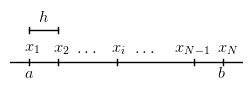
\includegraphics{./cap_pvc/pics/malha_uniforme/malha_uniforme}
  \caption{Malha uniforme de $N$ pontos em um intervalo $[a, b]$.}
  \label{fig:malha_uniforme}
\end{figure}

{\bf 1. Construção da malha.} A malha consiste em uma representação discreta do domínio $[a, b]$. Como veremos, sua construção tem impacto direto nas próximas etapas do método. Aqui, vamos construir a malha mais simples possível, aquela que consiste de $N$ pontos igualmente espaçados, isto é, a chamada \emph{malha uniforme}\index{malha uniforme}.

Para tanto, seja $N\in\mathbb{N}$ dado e, então, tomamos o seguinte conjunto discreto $\mathcal{P}_N = \{x_1, x_2, \dotsc, x_N\}$ (a malha), onde
\begin{equation}
  x_i = a + (i-1)h,\quad i=1, 2, \dotsc, N,
\end{equation}
com
\begin{equation}
  h:=\frac{b-a}{N-1},
\end{equation}
o qual é chamado de \emph{tamanho (ou passo) da malha}\index{tamanho da malha}\index{passo da malha} (veja a Figura~\ref{fig:malha_uniforme}).

{\bf 2. Construção do problema discreto.}\index{problema discreto} A segunda etapa consiste na discretização das equações, no nosso caso, das equações \eqref{eq:pvc1-eq}-\eqref{eq:pvc1-bc2}. 

Vamos começar pela Equação~\eqref{eq:pvc1-eq}. Em um ponto da malha $x_i$, $i = 2, 3, \dotsc, N-1$, temos
\begin{equation}
  -u_{xx}(x_i) = f(x_i, u(x_i)).
\end{equation}
Usando a fórmula de diferenças finitas central de ordem 2 para a segunda derivada, temos
\begin{equation}
  -\left(\frac{u(x_i-h) - 2u(x_i) + u(x_i+h)}{h^2} + O(h^2)\right) = f(x_i, u(x_i)).
\end{equation}
Rearranjando os termos, obtemos
\begin{equation}
  -\frac{u(x_i-h) - 2u(x_i) + u(x_i+h)}{h^2} = f(x_i, u(x_i)) + O(h^2). 
\end{equation}

Agora, denotando por $u_i$ a aproximação numérica de $u(x_i)$, a equação acima nos fornece
\begin{equation}\label{eq:pvc1-disc-eq}
\frac{1}{h^2}u_{i-1} - \frac{2}{h^2}u_i + \frac{1}{h^2}u_{i+1} = -f(x_i, u_i),
\end{equation}
para $i=2, 3, \dotsc, N-1$. Observamos que trata-se de um sistema de $N$ incógnitas, a saber $u_i$, e de $N-2$ equações, isto é, um sistema subdeterminado.

Para obtermos um sistema determinado, aplicamos as condições de contorno. Da condição de contorno dada na Equação~\eqref{eq:pvc1-bc1}, temos
\begin{equation}\label{eq:pvc1-disc-bc1}
  u(a) = u_a\Rightarrow u_1 = u_a.
\end{equation}
Analogamente, da condição de contorno dada na Equação~\eqref{eq:pvc1-bc1}, temos
\begin{equation}\label{eq:pvc1-disc-bc2}
  u(b) = u_b\Rightarrow u_N = u_b.
\end{equation}

Por fim, as equações \eqref{eq:pvc1-disc-bc2}, \eqref{eq:pvc1-disc-eq} e \eqref{eq:pvc1-disc-bc1} determinam o problema discreto associado
\begin{eqnarray}
  u_1 &=& u_a,\label{eq:pvc1-disc-eq1}\\
  \frac{1}{h^2}u_{i-1} - \frac{2}{h^2}u_i + \frac{1}{h^2}u_{i+1} &=& -f(x_i, u_i),\quad i=2, \dotsc, N-1,\label{eq:pvc1-disc-eqi}\\
  u_N &=& u_b.\label{eq:pvc1-disc-eqN}
\end{eqnarray}
Este é um sistema de equações de $N$ incógnitas e $N$ equações.

{\bf 3. Resolução do sistema discreto.} Esta etapa consiste em resolver o sistema discreto construído na etapa anterior. 

Para o PVC \eqref{eq:pvc1-eq}-\eqref{eq:pvc1-bc2}, construímos o problema discreto \eqref{eq:pvc1-disc-eq1}-\eqref{eq:pvc1-disc-eqN}. Este é um problema de $N$ equações e $N$ incógnitas. Observamos que se $f(x, u)$ é uma função linear, o sistema será linear e podemos resolver o sistema usando de técnicas numéricas para sistema lineares. Agora, se $f(x, u)$ é uma função não linear, podemos usar, por exemplo, do método de Newton para sistemas.

{\bf 4. Visualização e interpretação dos resultados.} A solução do problema discreto consiste dos valores $u_i$, isto é, de aproximações dos valores de $u$ nos pontos da malha. Para visualizarmos a solução podemos, por exemplo, construir o gráfico do conjunto de pontos $\{(x_i, u_i)\}$. Ainda, para obtermos aproximações da solução em outros pontos que não fazem parte da malha, podemos usar de técnicas de interpolação e/ou ajuste.

\begin{ex}\label{ex:pvc2}
  Use o método de diferenças finitas para resolver o seguinte problema de valor de contorno com condições de Dirichlet homogêneas:
  \begin{eqnarray}
    -u_{xx} &=& 100(x-1)^2,\quad 0 < x < 1,\label{eq:pvc2-eq}\\
    u(0) &=& 0,\label{eq:pvc2-bc1}\\
    u(1) &=& 0.\label{eq:pvc2-bc2}
  \end{eqnarray}
Use a fórmula de diferenças finitas central de ordem 2 para discretizar a derivada em uma malha uniforme de 11 pontos. Calcule, também, a solução analítica deste problema, faça um esboço das soluções numérica e analítica e compute o erro absoluto médio definido por
\begin{equation}
  E := \frac{1}{N}\sum_{i=1}^N \left|u(x_i) - u_i\right|,
\end{equation}
onde $x_i$ é o $i$-ésimo ponto da malha, $i=1, 2, \dotsc, N$ e $N$ é o número de pontos na mesma. Por fim, repita seus cálculos para uma malha com $101$ pontos. O que ocorre com o erro absoluto médio?
\end{ex}
\begin{sol} Vamos seguir as etapas conforme acima.

  {\bf 1. Construção da malha.} Tomando $N=11$, definimos os pontos da malha no domínio [0, 1] por:
  \begin{equation}
    x_i = (i-1)h,\quad i=1, 2, \dotsc, N,
  \end{equation}
com $h = 1/(N-1)$.

%%%%%%%%%%%%%%%%%%%%
% scilab
%%%%%%%%%%%%%%%%%%%%
\ifisscilab
No \verb+Scilab+, podemos construir a malha da seguinte forma:
\begin{verbatim}
a = 0
b = 1
N = 11
h = (b-a)/(N-1)
x = linspace(a,b,N)
\end{verbatim}
\fi
%%%%%%%%%%%%%%%%%%%%
%%%%%%%%%%%%%%%%%%%%
% octave
%%%%%%%%%%%%%%%%%%%%
\ifisoctave
No \verb+GNU Octave+, podemos construir a malha da seguinte forma:
\begin{verbatim}
a = 0
b = 1
N = 11
h = (b-a)/(N-1)
x = linspace(a,b,N)
\end{verbatim}
\fi
%%%%%%%%%%%%%%%%%%%%
%%%%%%%%%%%%%%%%%%%%
% python
%%%%%%%%%%%%%%%%%%%%
\ifispython
Em \verb+Python+, podemos construir a malha da seguinte forma:
\begin{verbatim}
a = 0
b = 1
N = 11
h = (b-a)/(N-1)
x = np.linspace(a,b,N)
\end{verbatim}
\fi
%%%%%%%%%%%%%%%%%%%%

{\bf 2. Construção do problema discreto.} Usando a fórmula de diferenças finitas central de ordem 2 para aproximar a derivada na Equação~\eqref{eq:pvc2-eq}, obtemos o seguinte sistema de equações:
\begin{equation}
  - \frac{u_{i-1} - 2u_i + u_{i+1}}{h^2} = 100(x_i - 1)^2,\quad i = 2, \dotsc, N-1.
\end{equation}
Completamos este sistema com as condições de contorno dadas nas equações~\eqref{eq:pvc2-bc1} e \eqref{eq:pvc2-bc2}, donde
\begin{equation}
  u_1 = u_N = 0.
\end{equation}
Ou seja, obtemos o seguinte problema discreto:
\begin{eqnarray}
  u_1 &=& 0,\label{eq:pvc2_disc_bc1}\\
  -\frac{1}{h^2}\left(u_{i-1} - 2u_i + u_{i+1}\right) &=& 100(x_i-1)^2,\quad i=2, \dotsc, N-1,\\
  u_N &=& 0.\label{eq:pvc2_disc_bc2}
\end{eqnarray}
Observamos que este é um sistema linear $N\times N$, o qual pode ser escrito na forma matricial $A\underline{u} = b$, cujos matriz de coeficientes é
\begin{equation}
  A = 
  \begin{bmatrix}
    1 & 0 & 0 & 0 & 0 & \cdots & 0\\
    1 & -2 & 1 & 0 & 0 & \cdots & 0\\
    0 & 1 & -2 & 1 & 0 & \cdots & 0\\
    \vdots & \vdots & \vdots & \vdots & \vdots & \vdots & \vdots\\
    0 & 0 & 0 & 0 & 0 & \cdots & 1
  \end{bmatrix},
\end{equation}
o vetor das incógnitas e o vetor dos termos constantes são
\begin{equation}
  \underline{u} =
  \begin{bmatrix}
    u_1\\
    u_2\\
    u_3\\
    \vdots\\
    u_N
  \end{bmatrix}\quad\text{e}\quad
  b =
  \begin{bmatrix}
    0\\
    -100h^{2}(x_2-1)^2\\
    -100h^{2}(x_3-1)^2\\
    \vdots\\
    0
  \end{bmatrix}.
\end{equation}

%%%%%%%%%%%%%%%%%%%%
% scilab
%%%%%%%%%%%%%%%%%%%%
\ifisscilab
No \verb+Scilab+, podemos construir o problema discreto a seguinte forma:
\begin{verbatim}
A = zeros(N,N)
b = zeros(N)

A(1,1) = 1
b(1) = 0
for i = 2:N-1
    A(i,i-1) = 1
    A(i,i) = -2
    A(i,i+1) = 1
    b(i) = -100 * h^2 * (x(i)-1)^2
end
A(N,N) = 1
b(N) = 0
\end{verbatim}
\fi
%%%%%%%%%%%%%%%%%%%%
%%%%%%%%%%%%%%%%%%%%
% octave
%%%%%%%%%%%%%%%%%%%%
\ifisoctave
No \verb+GNU Octave+, podemos construir o problema discreto a seguinte forma:
\begin{verbatim}
A = zeros(N,N)
b = zeros(N)

A(1,1) = 1
b(1) = 0
for i = 2:N-1
    A(i,i-1) = 1
    A(i,i) = -2
    A(i,i+1) = 1
    b(i) = -100 * h^2 * (x(i)-1)^2
end
A(N,N) = 1
b(N) = 0
\end{verbatim}
\fi
%%%%%%%%%%%%%%%%%%%%
%%%%%%%%%%%%%%%%%%%%
% python
%%%%%%%%%%%%%%%%%%%%
\ifispython
Em \verb+Python+, podemos construir o problema discreto a seguinte forma:
\begin{verbatim}
A = np.zeros((N,N))
b = np.zeros(N)

A[0,0] = 1
b[0] = 0
for i in np.arange(1,N-1):
    A[i,i-1] = 1
    A[i,i] = -2
    A[i,i+1] = 1
    b[i] = -100 * h**2 * (x[i]-1)**2
A[N-1,N-1] = 1
b[N-1] = 0
\end{verbatim}
\fi
%%%%%%%%%%%%%%%%%%%%

{\bf 3. Resolução do problema discreto.} Neste caso, o problema discreto consiste no sistema linear $A\underline{u} = b$ e, portanto, a solução é
\begin{equation}\label{eq:pvc2_numerica}
  \underline{u} = A^{-1}b.
\end{equation}

%%%%%%%%%%%%%%%%%%%%
% scilab
%%%%%%%%%%%%%%%%%%%%
\ifisscilab
No \verb+Scilab+, podemos computar a solução do sistema $A\underline{u} = b$ com:
\begin{verbatim}
u = A\b
\end{verbatim}
\fi
%%%%%%%%%%%%%%%%%%%%
%%%%%%%%%%%%%%%%%%%%
% octave
%%%%%%%%%%%%%%%%%%%%
\ifisoctave
No \verb+GNU Octave+, podemos computar a solução do sistema $A\underline{u} = b$ com:
\begin{verbatim}
u = A\b
\end{verbatim}
\fi
%%%%%%%%%%%%%%%%%%%%
%%%%%%%%%%%%%%%%%%%%
% python
%%%%%%%%%%%%%%%%%%%%
\ifispython
Em \verb+Python+, podemos computar a solução do sistema $A\underline{u} = b$ com:
\begin{verbatim}
u = np.linalg.solve(A,b)
\end{verbatim}
\fi
%%%%%%%%%%%%%%%%%%%%

\begin{figure}
  \centering
  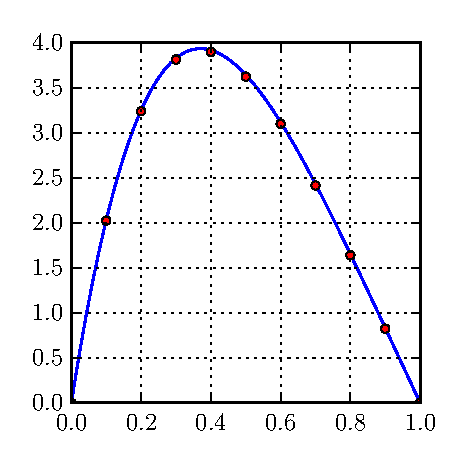
\includegraphics{./cap_pvc/pics/ex_pvc2/ex_pvc2}
  \caption{Esboço dos gráficos das soluções analítica (linha) e numérica (pontos) do PVC dado no Exemplo~\ref{ex:pvc2}.}
  \label{fig:ex_pvc2}
\end{figure}

{\bf 4. Visualização e interpretação dos resultados.} Tendo resolvido o problema discreto $A\underline{u} = b$, obtemos os valores da solução numérico de $u$ nos pontos da malha, isto é, obtivemos o conjunto de pontos $\{(x_i, u_i)\}_{i=1}^N$. Neste exemplo, queremos comparar a solução numérica com a solução analítica.

A solução analítica pode ser obtida por integração. Temos:
\begin{equation}
  \begin{split}
    -u_{xx} = 100(x-1)^2 &\Rightarrow -u_x + c_1 = 100\frac{(x-1)^3}{3}\\
    \Rightarrow -u + c_2x + c_1 = 100\frac{(x-1)^4}{12},
  \end{split}
\end{equation}
ou seja, $\displaystyle u(x) = - \frac{(x-1)^4}{12} + c_2x + c_1$. As constantes são determinadas pelas condições de contorno dadas pelas equações~\eqref{eq:pvc2-bc1} e \eqref{eq:pvc2-bc2}, isto é:
\begin{equation}
  \begin{split}
    u(0) = 0 &\Rightarrow c_1 = \frac{100}{12},\\
    u(1) = 0 &\Rightarrow c_2 = -\frac{100}{12}.
  \end{split}
\end{equation}
Portanto, a solução analítica é:
\begin{equation}\label{eq:pvc2_analitica}
  u(x) = -100\frac{(x-1)^4}{12} - 100\frac{x}{12} + \frac{100}{12}
\end{equation}

A Figura~\ref{fig:ex_pvc2} mostra o esboço dos gráficos das soluções analítica \eqref{eq:pvc2_analitica} e a da solução numérica \eqref{eq:pvc2_numerica}.

%%%%%%%%%%%%%%%%%%%%
% scilab
%%%%%%%%%%%%%%%%%%%%
\ifisscilab
No \verb+Scilab+, podemos fazer o esboço das soluções analítica e numérica da seguinte forma:
\begin{verbatim}
//def. sol. analitica
deff('y = ue(x)','y = -100.0*(x-1).^4/12 - 100*x/12 + 100.0/12')

//gráfico
xx = linspace(0,1)
yy = ue(xx)

plot(x,u,'ro',xx,yy,'b-')
\end{verbatim}
\fi
%%%%%%%%%%%%%%%%%%%%
%%%%%%%%%%%%%%%%%%%%
% octave
%%%%%%%%%%%%%%%%%%%%
\ifisoctave
No \verb+GNU Octave+, podemos fazer o esboço das soluções analítica e numérica da seguinte forma:
\begin{verbatim}
#def. sol. analitica
ue = inline("-100.0*(x-1).^4/12 - 100*x/12 + 100.0/12")

#gráfico
xx = linspace(0,1)
yy = ue(xx)

plot(x,u,'ro',xx,yy,'b-')
\end{verbatim}
\fi
%%%%%%%%%%%%%%%%%%%%
%%%%%%%%%%%%%%%%%%%%
% python
%%%%%%%%%%%%%%%%%%%%
\ifispython
Em \verb+Python+, podemos fazer o esboço das soluções analítica e numérica da seguinte forma:
\begin{verbatim}
#def. sol. analitica
def ue(x):
    return -100.0*(x-1)**4/12 - 100*x/12 + 100.0/12

#gráfico
xx = np.linspace(0,1)
yy = np.zeros(50)
for i,xxi in enumerate(xx):
    yy[i] = ue(xxi)

plt.plot(x',u,'ro',xx,yy,'b-')
plt.show()
\end{verbatim}
\fi
%%%%%%%%%%%%%%%%%%%%

\begin{table}
  \centering
  \caption{Erro absoluto médio das soluções numéricas com $N=11$ e $N=101$ do PVC dado no Exemplo~\ref{ex:pvc2}.}
  \begin{tabular}{ll|c}
    $N$ & $h$ & $E$\\\hline
    11 & 0,1 & $1,3\times 10^{-2}$\\
    101 & 0,01 & $1,4\times 10^{-4}$
  \end{tabular}
  \label{tab:pvc2_erro}
\end{table}

Por fim, computamos o erro absoluto médio das soluções numéricas com $N=11$ e $N=101$. A Tabela~\ref{tab:pvc2_erro} mostra os resultados obtidos. Observamos, que ao diminuirmos $10$ vezes o tamanho do passo $h$, o erro absoluto médio diminui aproximadamente $100$ vezes. Este resultado é esperado, pois o problema discreto \eqref{eq:pvc2_disc_bc1}-\eqref{eq:pvc2_disc_bc2} aproxima o problema contínuo \eqref{eq:pvc2-eq}-\eqref{eq:pvc2-bc2} com erro de truncamento de ordem $h^2$. Verifique!

%%%%%%%%%%%%%%%%%%%%
% scilab
%%%%%%%%%%%%%%%%%%%%
\ifisscilab
No \verb+Scilab+, podemos computar o erro absoluto médio da seguinte forma:
\begin{verbatim}
E = sum(abs(ue(x)' - u))/N
\end{verbatim}
\fi
%%%%%%%%%%%%%%%%%%%%
%%%%%%%%%%%%%%%%%%%%
% octave
%%%%%%%%%%%%%%%%%%%%
\ifisoctave
No \verb+GNU Octave+, podemos computar o erro absoluto médio da seguinte forma:
\begin{verbatim}
E = sum(abs(ue(x)' - u))/N
\end{verbatim}
\fi
%%%%%%%%%%%%%%%%%%%%
%%%%%%%%%%%%%%%%%%%%
% python
%%%%%%%%%%%%%%%%%%%%
\ifispython
Em \verb+Python+, podemos computar o erro absoluto médio da seguinte forma:
\begin{verbatim}
E = 0
for i,xi in enumerate(x):
    E += np.abs(ue(xi) - u[i])
E /= N
\end{verbatim}
\fi
%%%%%%%%%%%%%%%%%%%%
\end{sol}

\subsection*{Exercícios resolvidos}

\begin{exeresol}\label{exeresol:pvc_linear} Use o método de diferenças finitas para resolver o seguinte problema de valor de contorno:
  \begin{eqnarray}
    -u_{xx} + u  &=& e^{-x},\quad 0<x<1,\\
    u(0,5) &=& 1,\\
    u(1,5) &=& 2.
  \end{eqnarray}
Para tanto, use a fórmula de diferenças finitas central de ordem 2 para discretizar a derivada em uma malha uniforme com passo $h=0,1$. Faça, então, um esboço do gráfico da solução computada.
\end{exeresol}
\begin{resol}
O passo $h$ é uma malha uniforme com $N$ pontos no domínio $[0,5, 1,5]$ satisfaz:
\begin{equation}
  h = \frac{(b-a)}{N-1} \Rightarrow N = \frac{(b-a)}{h} + 1.
\end{equation}
Ou seja, a malha deve conter $N = 11$ pontos igualmente espaçados. Denotamos os pontos na malha por $x_i$, onde $x_i = 0,5 + (i-1)h$.

\begin{table}
  \centering
  \begin{tabular}{cc|cc}
    $x$ & $u$ & $x$ & $u$\\\hline
0.50 & 1.000000 & 1.00 & 1.643900 \\
0.60 & 1.143722 & 1.10 & 1.745332 \\
0.70 & 1.280661 & 1.20 & 1.834176 \\
0.80 & 1.410269 & 1.30 & 1.908160 \\
0.90 & 1.531724 & 1.40 & 1.964534 \\
1.00 & 1.643900 & 1.50 & 2.000000 \\\hline
  \end{tabular}
  \caption{Solução numérica do Exercício~\ref{exeresol:pvc_linear}.}
  \label{tab:exeresol_pvc_linear}
\end{table}

Agora, a equação diferencial dada no $i$-ésimo ponto da malha é:
\begin{equation}
  -u_{xx}(x_i) + u(x_i) = e^{x_i},\quad i = 2, 3, \dotsc, N-1.
\end{equation}
Denotando $u_i \approx u(x_i)$ e usando a fórmula de diferenças finitas central de ordem dois para a derivada $u_{xx}$, obtemos:
\begin{equation}
  -\left(\frac{u_{i-1} - 2u_i + u_{i+1}}{h^2}\right) + u_i = e^{x_i},
\end{equation}
para $i= 2, 3, \dotsc, N-1$. Rearranjando os termos e aplicando as condições de contorno, temos o problema discretizado como segue:
\begin{equation}
  \begin{split}
    u_1 &= 1\\
    -u_{i-1} + (2 + h^2)u_i - u_{i+1} &= h^2e^{x_i},\quad i=2 ,\dotsc, N-1,\\
    u_N &= 2.
  \end{split}
\end{equation}

\begin{figure}
  \centering
  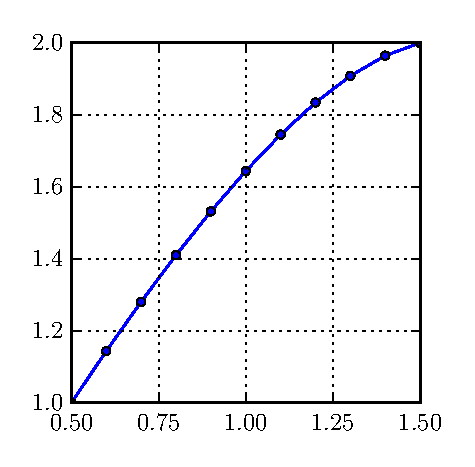
\includegraphics{./cap_pvc/pics/exeresol_pvc_linear/exeresol_pvc_linear}
  \caption{Esboço do gráfico da solução numérica do Exercício~\ref{exeresol:pvc_linear}.}
  \label{fig:exeresol_pvc_linear}
\end{figure}

O problema discreto obtido é um sistema linear $N\times N$. Resolvendo este sistema, obtemos a solução discreta apresentada na Tabela~\ref{tab:exeresol_pvc_linear}. A Figura~\ref{fig:exeresol_pvc_linear} mostra um esboço do gráfico da solução computada.

%%%%%%%%%%%%%%%%%%%%
% scilab
%%%%%%%%%%%%%%%%%%%%
\ifisscilab
No \verb+Scilab+, podemos computar a solução numérica e graficá-la com o seguinte código:
\begin{verbatim}
//malha
a = 0.5
b = 1.5
N = 11
h = (b-a)/(N-1)
x = linspace(a,b,N)'

//sistema
A = zeros(N,N)
b = zeros(N,1)

A(1,1) = 1
b(1) = 1
for i = 2:N-1
    A(i,i-1) = -1
    A(i,i) = 2 + h^2
    A(i,i+1) = -1
    b(i) = h^2 * exp(x(i))
end
A(N,N) = 1
b(N) = 2

//solucao
u = A\b

//gráfico
plot(x,u,'b-o')
\end{verbatim}
\fi
%%%%%%%%%%%%%%%%%%%%
%%%%%%%%%%%%%%%%%%%%
% octave
%%%%%%%%%%%%%%%%%%%%
\ifisoctave
No \verb+GNU Octave+, podemos computar a solução numérica e graficá-la com o seguinte código:
\begin{verbatim}
#malha
a = 0.5
b = 1.5
N = 11
h = (b-a)/(N-1)
x = linspace(a,b,N)'

#sistema
A = zeros(N,N)
b = zeros(N,1)

A(1,1) = 1
b(1) = 1
for i = 2:N-1
    A(i,i-1) = -1
    A(i,i) = 2 + h^2
    A(i,i+1) = -1
    b(i) = h^2 * exp(x(i))
endfor
A(N,N) = 1
b(N) = 2

#solucao
u = A\b

#gráfico
plot(x,u,'b-o')
\end{verbatim}
\fi
%%%%%%%%%%%%%%%%%%%%
%%%%%%%%%%%%%%%%%%%%
% python
%%%%%%%%%%%%%%%%%%%%
\ifispython
Em \verb+Python+, podemos computar a solução numérica e graficá-la com o seguinte código:
\begin{verbatim}
#malha
a = 0.5
b = 1.5
N = 11
h = (b-a)/(N-1)
x = np.linspace(a,b,N)

#sistema
A = np.zeros((N,N))
b = np.zeros(N)

A[0,0] = 1
b[0] = 1
for i in np.arange(1,N-1):
    A[i,i-1] = -1
    A[i,i] = 2 + h**2
    A[i,i+1] = -1
    b[i] = h**2 * np.exp(x[i])
A[N-1,N-1] = 1
b[N-1] = 2

#solucao
u = np.linalg.solve(A,b)

#gráfico
plt.plot(x,u,'b-o')
plt.show()
\end{verbatim}
\fi
%%%%%%%%%%%%%%%%%%%%
\end{resol}

\subsection*{Exercícios}

\begin{exer}
 Considere o seguinte problema de valor de contorno para a equação de calor no estado estacionário:
\begin{equation}\left\{\begin{array}{l}-u_{xx}=32,~~ 0<x<1.\\
u(0)=5\\
u(1)=10\end{array}
\right.
\end{equation}

Defina $u_j=u(x_j)$ onde $x_j={(j-1)}{h}$ e $j=1,\ldots,5$. Aproxime a derivada segunda por um esquema de segunda ordem e transforme a equação diferencial em um sistema de equações lineares. Escreva este sistema linear na forma matricial e resolva-o. Faça o mesmo com o dobro de subintervalos, isto é, com malha de 9 pontos. 
\end{exer}
\begin{resp}
 \begin{equation}\left[
  \begin{array}{ccccc}
         1 & 0& 0& 0& 0\\
         -1 & 2 & -1 &0&0\\
         0&-1 & 2 & -1 &0\\
         0&0&-1 & 2 & -1 \\
         0 & 0& 0& 0& 1\\
        \end{array}
\right]
\left[
  \begin{array}{c}
     u_1\\ u_2\\u_3\\u_4 \\ u_5
   \end{array}
\right]
=
\left[
  \begin{array}{c}
     5\\ 2\\2\\2 \\ 10
   \end{array}
\right]
\end{equation}


Solução:  [5, 9.25, 11.5, 11.75, 10]    

\begin{equation}\left[
  \begin{array}{ccccccccc}
         1 & 0& 0& 0& 0& 0& 0& 0& 0\\
         -1 & 2 & -1 &0&0& 0& 0& 0& 0\\
         0&-1 & 2 & -1 &0& 0& 0& 0& 0\\
         0&0&-1 & 2 & -1 & 0& 0& 0& 0\\
         0&0&0&-1 & 2 & -1 & 0& 0& 0\\
         0&0&0&0&-1 & 2 & -1 & 0& 0\\
         0&0&0&0&0&-1 & 2 & -1 & 0\\
         0&0&0&0&0&0&-1 & 2 & -1\\
         0 & 0& 0& 0& 0& 0& 0& 0& 1\\
        \end{array}
\right]
\left[
  \begin{array}{c}
     u_1\\ u_2\\u_3\\u_4 \\u_5\\ u_6\\u_7\\u_8\\u_9
   \end{array}
\right]
=
\left[
  \begin{array}{c}
     5\\ 0.5\\0.5\\0.5\\ 0.5\\0.5\\0.5\\0.5 \\ 10
   \end{array}
\right]
\end{equation}

Solução:  $[5, 7.375, 9.25, 10.625, 11.5, 11.875, 11.75, 1.125, 10]$
\end{resp}


\begin{exer} Considere o seguinte problema de valor de contorno para a equação de calor no estado estacionário:
\begin{equation}\left\{\begin{array}{l}-u_{xx}=200e^{-(x-1)^2},~~ 0<x<2.\\
u(0)=120\\
u(2)=100\end{array}
\right.
\end{equation}
Defina $u_j=u(x_j)$ onde $x_j={(j-1)}{h}$ e $j=1,\ldots,21$. Aproxime a derivada segunda por um esquema de segunda ordem e transforme a equação diferencial em um sistema de equações lineares. Resolva o sistema linear obtido.
\end{exer}
\begin{resp}
120.    133.56    146.22    157.83    168.22    177.21    184.65    190.38    194.28    196.26    196.26    194.26    190.28    184.38    176.65    167.21  156.22    143.83    130.22    115.56    100.    
\end{resp}

\begin{exer} Considere o seguinte problema de valor de contorno para a equação de calor no estado estacionário:
\begin{equation}\left\{\begin{array}{l}-u_{xx}=200e^{-(x-1)^2},~~ 0<x<2.\\
u'(0)=0\\
u(2)=100\end{array}
\right.
\end{equation}
Defina $u_j=u(x_j)$ onde $x_j={(j-1)}{h}$ e $j=1,\ldots,21$. Aproxime a derivada segunda por um esquema de segunda ordem, a derivada primeira na fronteira por um esquema de primeira ordem e transforme a equação diferencial em um sistema de equações lineares. Resolva o sistema linear obtido.
\end{exer}
\begin{resp}
391.13    391.13    390.24    388.29    385.12    380.56    374.44    366.61    356.95    345.38    331.82    316.27    298.73    279.27    257.99    234.99    210.45    184.5    157.34    129.11    100.    
\end{resp}


\begin{exer} Considere o seguinte problema de valor de contorno para a equação de calor no estado estacionário com um termo não linear de radiação:
\begin{equation}\left\{\begin{array}{l}-u_{xx}=100- \frac{u^4}{10000},~~ 0<x<2.\\
u(0)=0\\
u(2)=10\end{array}
\right.
\end{equation}
Defina $u_j=u(x_j)$ onde $x_j={(j-1)}{h}$ e $j=1,\ldots,21$. Aproxime a derivada segunda por um esquema de segunda ordem e transforme a equação diferencial em um sistema de equações não lineares. Resolva o sistema  obtido. Expresse  a solução com dois algarismos depois do separador decimal. Dica: Veja problema 38 da lista 2, seção de sistemas não lineares.
\end{exer}
\begin{resp}
0.,    6.57,    12.14,    16.73,    20.4,    23.24,    25.38,    26.93 ,   28,    28.7,    29.06,    29.15,    28.95,    28.46, 27.62 ,   26.36,    24.59,    22.18,    19.02,    14.98,    10.    
\end{resp}

\begin{exer} Considere o seguinte problema de valor de contorno para a equação de calor no estado estacionário com um termo não linear de radiação e um termo de convecção:
\begin{equation}\left\{\begin{array}{l}-u_{xx}+3u_x=100- \frac{u^4}{10000},~~ 0<x<2.\\
u'(0)=0\\
u(2)=10\end{array}
\right.
\end{equation}
Defina $u_j=u(x_j)$ onde $x_j={(j-1)}{h}$ e $j=1,\ldots,21$. Aproxime a derivada segunda por um esquema de segunda ordem, a derivada primeira na fronteira por um esquema de primeira ordem, a derivada primeira no interior por um esquema de segunda ordem e transforme a equação diferencial em um sistema de equações não lineares. Resolva o sistema  obtido.
\end{exer}
\begin{resp}
$u(0)=31.62$, $u(1)=31,50$, $u(1,9)=18,17$.    
\end{resp}

\begin{exer} Considere o seguinte problema de valor de contorno:
\begin{equation}\left\{\begin{array}{l}-u''+2u'=e^{-x}- \frac{u^2}{100},~~ 1<x<4.\\
u'(1)+u(1)=2\\
u'(4)=-1\end{array}
\right.
\end{equation}
Defina $u_j=u(x_j)$ onde $x_j=1+{(j-1)}{h}$ e $j=1,\ldots,101$. Aproxime a derivada segunda por um esquema de segunda ordem, a derivada primeira na fronteira por um esquema de primeira ordem, a derivada primeira no interior por um esquema de segunda ordem e transforme a equação diferencial em um sistema de equações não lineares. Resolva o sistema  obtido.
\end{exer}
\begin{resp}
$u(1)=1,900362$, $u(2,5)=1.943681$, $u(4)=1,456517$.    
\end{resp}

%\end{document} 

%

 %Este está licenciado sob a Licença Creative Commons Atribuição-CompartilhaIgual 3.0 Não Adaptada. Para ver uma cópia desta licença, visite https://creativecommons.org/licenses/by-sa/3.0/ ou envie uma carta para Creative Commons, PO Box 1866, Mountain View, CA 94042, USA.

%\documentclass[main.tex]{subfiles}
%\begin{document}

\chapter{Problemas de valor inicial}\index{problema de valor inicial}
Neste capítulo, vamos estudar metodologias numéricas para aproximar a solução de problema de valor inicial (PVI) para equações diferenciais ordinárias. Primeiramente, daremos atenção aos problemas de primeira ordem e, depois, mostraremos que estas técnicas podem ser estendidas para problemas e sistemas de ordem superior. Considere um problema de valor inicial de primeira ordem dado por:
\begin{subequations}\label{eq:PVI}
\begin{eqnarray}
  u'(t) &=& f(t, u(t)),~~t>t^{(1)}\label{eq:PVI_EDO}\\
  u(t^{(1)}) &=& a ~~ \text{(condição inicial)}.\label{eq:PVI_CI}
\end{eqnarray}
\end{subequations}

A incógnita de um problema de valor inicial é uma função que satisfaz a equação diferencial \eqref{eq:PVI_EDO} e a condição inicial \eqref{eq:PVI_CI}.

Considere os próximos três exemplos:
\begin{ex} O seguinte problema é linear não homogêneo:
\begin{equation}
\begin{split}
    u'(t) &=t\\
   u(0) &= 2
   \end{split}
   \end{equation}
\end{ex}

\begin{ex} O seguinte problema é linear homogêneo:
\begin{eqnarray}
   u'(t) &=u(t)\\
            u(0) &= 1
\end{eqnarray}
\end{ex}

\begin{ex} O seguinte problema é não linear e não homogêneo:
\begin{eqnarray}
   u'(t) &=&\sin(u(t)^2+\sin(t))\\
            u(0) &=& a
\end{eqnarray}
\end{ex}

A solução do primeiro exemplo é $u(t)=t^2/2+2$ pois satisfaz a equação diferencial e a condição inicial. A solução do segundo também é facilmente obtida: $u(t)=e^t$. Porém como podemos resolver o terceiro problema?

Para muitos problemas de valor inicial da forma \eqref{eq:PVI}, não é possível encontrar uma expressão analítica fechada, ou seja, sabe-se que a solução existe e é única, porém não podemos expressá-la em termos de funções elementares. Por isso é necessário calcular aproximações numéricas para a solução.

Existem uma enorme família de metodologias para construir soluções numéricas para problemas de valor inicial. Aqui, vamos nos limitar a estudar métodos que aproximam $u(t)$ em um conjunto finito de valores de $t$. Este conjunto de valores será chamado de \emph{malha} e será denotado por  $\{t^{(i)}\}_{i=1}^N=\{t^{(1)}, t^{(2)}, t^{(3)},\ldots, t^{(N)}\}$. Desta forma, aproximamos a solução $u(t^{(i)})$ por $u^{(i)}$ em cada ponto da malha usando diferentes esquemas numéricos.

%%%%%%%%%%%%%%%%%%%%
% python
%%%%%%%%%%%%%%%%%%%%
\ifispython
Nos códgos em \verb+Python+ apresentados neste capítulo, assumiremos que as seguintes bibliotecas e módulos estão importados:
\begin{verbatim}
import numpy as np
from numpy import linalg
import matplotlib.pyplot as plt
\end{verbatim}
\fi
%%%%%%%%%%%%%%%%%%%%e

\section{Rudimentos da teoria de problemas de valor inicial}
Uma questão fundamental no estudo dos problemas de valor iniciais consiste em analisar se um dado problema é um problema \emph{bem posto}. Ou seja,
\begin{itemize}
 \item Existe uma solução para o problema de valor inicial?
 \item A solução é única?
 \item A solução do problema de valor inicial é pouco sensível a pequenas perturbações nas condições iniciais?
\end{itemize}

A fim de responder tais questões, precisamos definir o conceito de função Lipschitz contínua, ou simplesmente, função Lipschitz \index{função!Lipschitz}
\begin{defn}
Uma função $f(t, u)$ é Lipschitz contínua em um intervalo $I$ em $u$ se existe uma constante $L$, tal que $\forall t \in [a, b]$ e $u, v \in \mathbb R$,
\begin{equation}  |f(t, u)-f(t, v)| \leq L|u-v|,~~\forall t\in I.  \end{equation}
\end{defn}

O seguinte resultado estabelece a existência e unicidade de solução para determinada classe de problemas de valor inicial:
\begin{teo}[Teorema de Picard-Lindelöf] Seja $f(t, u)$ contínua em $t$ e Lipschitz em $u$. Então o seguinte problema de valor inicial\index{teorema!de Picard-Lindelöf}
\begin{equation}\label{eq:pvi_picard}
  \begin{split}
    u'(t)  &= f(t, u(t)), \\
    u(t^{(1)}) &= a,
  \end{split}
\end{equation}
Admite uma única solução em um intervalo $[t^{(1)},t^{(f)})$ com $t^{(f)}>t^{(1)}.$
\end{teo}

% \begin{defn}
%   \emph{Estabilidade dinâmica} refere-se a propriedade de pequenas perturbações sobre o estado inicial de um sistema gerarem pequenas variações no estado final deste sistema (haverá decaimento nas variações, ou pelo menos não crescimento, quanto $t$ cresce).
% \end{defn}

\begin{teo}[Dependência contínua na condição inicial]
Se $u(t)$ e $v(t)$ são soluções do problema de valor inicial \eqref{eq:pvi_picard}, isto é, com $f(t, u)$ contínua em $t$ e Lipschitz em $u$ Lipschitz com $u(a)=u^{(1)}$, $v(a)=v^{(1)}$, então
\begin{equation}  |u(t)-v(t)| \leq  e^{L(t-t^{(1)})}|u^{(1)}-v_1|. \end{equation}
\end{teo}

\subsection*{Exercícios resolvidos}

\begin{exeresol} A função $f(t,u)=\sqrt{u},~~u\geq 0$ não é uma função Lipschitz em $u$, pois
\begin{equation} \lim_{u\to 0+} \frac{|f(t,u)-f(t,0)|}{|u-0|}=\lim_{u\to 0+} \frac{\sqrt{u}}{u}=\lim_{u\to 0+} \frac{1}{\sqrt{u}}=\infty \end{equation}
 Mostre que o seguinte problema de valor inicial não admite solução única:
\begin{eqnarray}
\frac{du}{dt} &=&\sqrt{u},~~u>0,\\
u(0) &=& 0.
\end{eqnarray}
\end{exeresol}
\begin{resol}
 A função identicamente nula, $u(t)=0$, satisfaz a equação diferencial e a condição de contorno, logo é uma solução do problema de valor inicial. No entanto, a função\footnote{Esta solução pode ser obtida por separação de variáveis.} $u(t)=\frac{t^2}{4}$ satisfaz a condição inicial, pois $u(0)=0$ e a equação diferencial pois $\frac{du}{dt}=\frac{t}{2}=\sqrt{\frac{t^2}{4}}$.

 De fato, qualquer função do tipo
 \begin{equation}u(t)=\left\{
 \begin{array}{ll}
  0,&0\leq t \leq t_0\\
  \frac{(t-t_0)^2}{4},& t >t_0\\
 \end{array}
 \right.\end{equation}
 é solução do problema de valor inicial dado.
\end{resol}

\subsection*{Exercícios}

\construirExer


\section{Método de Euler}\index{método!de Euler}\label{sec:euler}
Nesta seção, construiremos o mais simples dos métodos para resolver problemas de valor inicial: o método de Euler com passo constante.\index{Passo} Por passo constante, queremos dizer que os pontos da malha estão todos igualmente espaçados, isto é:
\begin{equation} t^{(i)}=(i-1)h,~~~i=1,2,\ldots,N. \end{equation}
onde $h$ é passo, ou seja, a distância entre dois pontos da malha.

Considere então o problema de valor inicial dado por:
\begin{equation}\label{eq:EDO1}
  \begin{split}
    u'(t)  &= f(t,u(t)),~~t>t^{(1)} \\
    u(t^{(1)}) &= a.
  \end{split}
\end{equation}
Ao invés de tentar solucionar o problema para qualquer $t>t^{(1)}$, iremos aproximar $u(t)$ em $t=t^{(2)}$.

Integrando \eqref{eq:EDO1} de $t^{(1)}$ até $t^{(2)}$, obtemos:
\begin{eqnarray}
  \int_{t^{(1)}}^{t^{(2)}} u'(t) \;dt &=& \int_{t^{(1)}}^{t^{(2)}} f(t,u(t)) \; dt\\
  u(t^{(2)})-u(t^{(1)})               &=& \int_{t^{(1)}}^{t^{(2)}} f(t,u(t)) \; dt\\
  u(t^{(2)})                      &=& u(t^{(1)}) +  \int _{t^{(1)}}^{t^{(2)}} f(t,u(t)) \; dt
\end{eqnarray}

Seja $u_n$ a aproximação de $u(t_n)$. Para obter o método numérico mais simples aproximamos $f$ em $[t^{(1)},t^{(2)}]$ pela função constante $f(t,u(t)) \approx  f(t^{(1)},u^{(1)})$,
\begin{eqnarray}
  u^{(2)} &=&  u^{(1)} +   f(t^{(1)},u^{(1)}) \int _{t^{(1)}}^{t^{(2)}}  \; dt \\
  u^{(2)} &=&  u^{(1)} +   f(t^{(1)},u^{(1)}) (t^{(2)}-t^{(1)}) \\
  u^{(2)} &=&  u^{(1)} + h f(t^{(1)},u^{(1)})
\end{eqnarray}

Este procedimento pode ser repetido para  $t^{(3)}$, $t^{(4)}$, $\ldots$, obtendo, assim, o chamado \emph{método de Euler}:
\begin{equation}\label{eq:euler}
  \begin{split}
    u^{(n+1)}&= u^{(n)} + h\;f(t^{(n)},u^{(n)}),\\
    u^{(1)}&= u^{(1)}=u(t^{(1)})~ \hbox{(condição inicial)}.
  \end{split}
\end{equation}


\begin{ex}
Considere o problema de valor inicial
\begin{equation}
 \begin{split}
  u'(t)&=2u(t)\\
  u(0)&=1
 \end{split}
\end{equation}

cuja solução é $u(t)=e^{2t}$. O método de Euler aplicado a este problema produz o  esquema:
\begin{equation}\label{eq:exemplo_y_2y_euler}
  \begin{split}
    u^{(k+1)}&= u^{(k)}+2hu^{(k)}=(1+2h)u^{(k)}\\
    u^{(1)}&= 1,
  \end{split}
\end{equation}
Suponha que queremos calcular o valor aproximado de $u(1)$ com $h=0,2$. Então os pontos $t^{(1)}=0$, $t^{(2)}=0,2$, $t^{(3)}=0,4$, $t^{(4)}=0,6$, $t^{(5)}=0,8$ e $t^{(6)}=1,0$ formam os seis pontos da malha. As aproximações para a solução nos pontos da malha usando o método de Euler são:
\begin{equation}
\begin{split}
  u(0)  &\approx u^{(1)}=1\\
  u(0,2)&\approx u^{(2)}=(1+2h) u^{(1)}=1,4 u^{(1)}=1,4\\
  u(0,4)&\approx u^{(3)}=1,4 u^{(2)}=1,96\\
  u(0,6)&\approx u^{(4)}=1,4 u^{(3)}=2,744\\
  u(0,8)&\approx u^{(5)}=1,4 u^{(4)}=3,8416\\
  u(1,0)&\approx u^{(6)}=1,4 u^{(5)}=5,37824
  \end{split}
\end{equation}
Essa aproximação é bem grosseira quando comparamos com a solução do problema em $t=1$: $u(1)=e^{2}\approx 7,38906$. Não obstante, se tivéssemos escolhido um passo menor, teríamos obtido uma aproximação melhor. Veja tabela abaixo com valores obtidos com diferentes valores de passo $h$.

\begin{tabular}{|l|l|l|l|l|l|l|l|}%\label{pvi:tab_euler}
\hline
   h&$10^{-1}$&$10^{-2}$&$10^{-3}$&$10^{-4}$&$10^{-5}$&$10^{-6}$&$10^{-7}$\\
   \hline
   $u^{(N)}$& 6,1917 &  6,7275 &  7,0400 &  7,2096  & 7,2980 &  7,3432  & 7,3660\\
   \hline
\end{tabular}

De fato, podemos mostrar que quando $h$ se aproxima de $0$, a solução aproximada via método de Euler converge para a solução exata $e^2$. Para isto, basta observar que a solução da relação de recorrência \eqref{eq:exemplo_y_2y_euler} é dada por
 \begin{equation} u^{(k)}=(1+2h)^{k-1}. \end{equation}
 Como $t^{(k)}=(k-1)h$ e queremos a solução em $t=2$, a solução aproximada pelo método de Euler com passo $h$ em é dada por:
 \begin{equation}
 u^{(k)}= (1+2h)^{k-1}= (1+2h)^{\frac{2}{h}}.
 \end{equation}
Aplicando o limite $h\to 0+$, temos:
  \begin{equation}
  \lim_{h\to 0+} (1+2h)^{\frac{2}{h}}= e^{2}.
  \end{equation}

%%%%%%%%%%%%%%%%%%%%
% python
%%%%%%%%%%%%%%%%%%%%
\ifispython
Em \verb+Python+, podemos computar a solução numérica deste problema de valor inicial via o método de Euler com o seguinte código:
\begin{verbatim}
#define f(t,u)
def f(t,u):
    return 2*u

#tamanho e num. de passos
h = 0.2
N = 6

#cria vetor t e u
t = np.empty(N)
u = np.copy(t)

#C.I.
t[0] = 0
u[0] = 1

#iteracoes
for i in np.arange(N-1):
    t[i+1] = t[i] + h
    u[i+1] = u[i] + h*f(t[i],u[i])

#imprime
for i,tt in enumerate(t):
    print("%1.1f %1.4f" % (t[i],u[i]))
\end{verbatim}
\fi
%%%%%%%%%%%%%%%%%%%%
\end{ex}

Vamos agora, analisar o desempenho do método de Euler usando um exemplo mais complicado, porém ainda simples suficiente para que possamos obter a solução exata:
\begin{ex}\label{ex:ex_euler_1}
Considere o problema de valor inicial relacionado à equação logística\index{equação!logística}:
\begin{equation}\label{eq:logistica}
  \begin{split}
    u'(t)&= u(t)(1-u(t))\\
    u(0)&= 1/2
  \end{split}
\end{equation}
\end{ex}
Podemos obter a solução exata desta equação usando o método de separação de variáveis\index{método!de separação de variáveis} e o método das frações parciais\index{método das frações parciais}. Para tal escrevemos:
\begin{equation}
\frac{du(t)}{u(t)(1-u(t))}=dt
\end{equation}
O termo $\frac{1}{u(t)(1-u(t))}$ pode ser decomposto em frações parciais como $\frac{1}{u}+\frac{1}{1-u}$ e chegamos na seguinte equação diferencial:
\begin{equation}
\left(\frac{1}{u(t)}+\frac{1}{1-u(t)}\right)du=dt.
\end{equation}
Integrando termo-a-termo, temos a seguinte equação algébrica relacionando $u(t)$ e $t$:
\begin{equation}
\ln(u(t))-\ln\left(1-u(t)\right)=t+C
\end{equation}
Onde $C$ é a constante de integração, que é definida pela condição inicial, isto é, $u=1/2$ em $t=0$. Substituindo, temos $C=0$. O que resulta em:
\begin{equation}
\ln\left(\frac{u(t)}{1-u(t)}\right)=t
\end{equation}
Equivalente a
\begin{equation}
\frac{u(t)}{1-u(t)}=e^{t} \Longrightarrow u(t)=(1-u(t))e^{t} \Longrightarrow (1+e^t)u(t)=e^{t}
\end{equation}
E, finalmente, encontramos a solução exata dada por $u(t)=\frac{e^t}{1+e^{t}}$.

Vejamos, agora, o esquema iterativo produzido pelo método de Euler:
\begin{equation}
 \begin{split}
u^{(k+1)}&= u^{(k)}+h u^{(k)}(1-u^{(k)}), \\
u^{(1)}&= 1/2.
 \end{split}
\end{equation}

\ifisscilab
O seguinte código pode ser usado para implementar no \verb+Scilab+ a recursão acima:
\begin{verbatim}
function u=euler(h,Tmax)
  u= .5;
  itmax = Tmax/h;
  for n=1:itmax
    u= u + h*u*(1-u);
   end
endfunction
\end{verbatim}
o qual pode ser invocado da seguinte forma $\left(h=1e-1, t=2\right)$:
\begin{verbatim}
-->euler(1e-1,2)
 ans  =

    0.8854273
\end{verbatim}

\fi

\ifisoctave
O seguinte código pode ser usado para implementar no \verb+Octave+ a recursão acima:
\begin{verbatim}
function u=euler(h,Tmax)
  u= .5;
  itmax = Tmax/h;
  for n=1:itmax
    u= u + h*u*(1-u);
   end
endfunction
\end{verbatim}
o qual pode ser invocado da seguinte forma $\left(h=1e-1, t=2\right)$:
\begin{verbatim}
>> euler(1e-1,1)
ans =  0.88543
\end{verbatim}
\fi


\ifispython
O seguinte código pode ser usado para implementar no \verb+Python+ a recursão acima:

\begin{verbatim}
def euler(h,Tmax):
	u=.5
  	itmax = Tmax/h;
	for i in np.arange(itmax):
		u = u + h*u*(1-u)
	return u


h=1e-1
for t in [.5, 1, 2, 3]:
	sol_euler=euler(h,t);
	sol_exata=1/(1+np.exp(-t))
	erro_relativo = np.fabs((sol_euler-sol_exata)/sol_exata)
	print("h=%1.0e - u(%1.1f) =~ %1.7f - erro_relativo = %1.1e" % (h, t, sol_euler, erro_relativo) )

h=1e-2
print;
for t in [.5, 1, 2, 3]:
	sol_euler=euler(h,t);
	sol_exata=1/(1+np.exp(-t))
	erro_relativo = np.fabs((sol_euler-sol_exata)/sol_exata)
	print("h=%1.0e - u(%1.1f) =~ %1.7f - erro_relativo = %1.1e" % (h, t, sol_euler, erro_relativo) )

\end{verbatim}
\fi
Para fins de comparação, calculamos a solução exata e aproximada para alguns valores de $t$ e de passo $h$ e resumimos na tabela abaixo:

%\begin{table}[h]
 % \caption{Tabela comparativa entre método de Euler e solução exata para Problema~\ref{ex_euler_1}.}
 % \label{tab:log}
  \begin{tabular}{|c|c|c|c|}\hline
    $t$ & $\text{Exato}$ & $\text{Euler}~~ h=0,1$ & $\text{Euler}~~ h=0,01$\\\hline
    $0$ & $1/2$ & $0,5$ & $0,5$\\\hline
    $1/2$ & $\frac{e^{1/2}}{1+e^{1/2}}\approx 0,6224593$ & $0,6231476$ & $0,6225316$\\\hline
    $1$ & $\frac{e}{1+e}\approx 0,7310586$ & $0,7334030$ & $0,7312946$\\\hline
    $2$ & $\frac{e^2}{1+e^2}\approx  0,8807971$ & $0,8854273$  & $0,8812533$ \\\hline
    $3$ & $\frac{e^3}{1+e^3}\approx   0,9525741$  & $0,9564754$ & $0,9529609$ \\\hline
  \end{tabular}
%\end{table}

\subsection*{Exercícios Resolvidos}

\begin{exeresol}\label{exeresol:exeresol1} Aproxime a solução do problema de valor inicial
\begin{eqnarray}
     u'(t)&=& -0,5u(t)+2+t\\
            u(0) &=&  8
\end{eqnarray}
Usando os seguintes passos: $h=10^{-1}$, $h=10^{-2}$, $h=10^{-3}$, $h=10^{-4}$ e $h=10^{-5}$ e compare a solução aproximada em $t=1$ com a solução exata dada por:
\begin{equation}
     u(t) = 2t+8e^{-t/2} \Longrightarrow u(1)=2+8e^{-1/2} \approx 6,85224527770107
\end{equation}
\end{exeresol}
\begin{resol} Primeramente itentificamos $f(t,u)=-0,5u+2+t$ e construímos o processo iterativo do método de Euler:
\begin{eqnarray}
  u^{(n+1)}&=&u^{(n)} + h( -0,5u^{(n)}+2+t^{(n)}),~~n=1,2,3,\ldots\\
  u^{(1)}&=&8
\end{eqnarray}

\ifisscilab
O seguinte código pode ser usado para implementar no \verb+Scilab+ a recursão acima:
\begin{verbatim}
function u=euler(h,Tmax)
  u= 8;
  t= 0;
  itmax = Tmax/h;
  for n=1:itmax
    t= (n-1)*h;
    u= u + h*(-0.5*u+2+t);
   end
endfunction
\end{verbatim}
o qual pode ser invocado da seguinte forma:
\begin{verbatim}
-->euler(1e-1,1)
 ans  =

    6.7898955
\end{verbatim}
Podemos construir um vetor com as cinco soluções da seguinte forma:
\begin{verbatim}
 -->S=[euler(1e-1,1) euler(1e-2,1) euler(1e-3,1) euler(1e-4,1) euler(1e-5,1)]
 S  =

    6.7898956   6.846163    6.851639    6.852185    6.8522392
\end{verbatim}

\fi

\ifisoctave
O seguinte código pode ser usado para implementar no \verb+Octave+ a recursão acima:
\begin{verbatim}
function u=euler(h,Tmax)
  u= 8;
  t= 0;
  itmax = Tmax/h;
  for n=1:itmax
    t= (n-1)*h;
    u= u + h*(-0.5*u+2+t);
   end
endfunction
\end{verbatim}
o qual pode ser invocado da seguinte forma:
\begin{verbatim}
>> euler(1e-1,1)
ans =  6.8799
\end{verbatim}
Podemos construir um vetor com as cinco soluções da seguinte forma:
\begin{verbatim}
 >> S=[euler(1e-1,1) euler(1e-2,1) euler(1e-3,1) euler(1e-4,1) euler(1e-5,1)]
S =

   6.7899   6.8462   6.8516   6.8522   6.8522
\end{verbatim}
\fi


\ifispython
O seguinte código pode ser usado para implementar no \verb+Python+ a recursão acima:

\begin{verbatim}
def euler(h,Tmax):
	u=8
  	itmax = Tmax/h;
	for i in np.arange(0,itmax):
		t=i*h
		k1 = -0.5*u+2+t
		u = u + h*k1
	return u


sol_exata = 2+8*np.exp(-.5)
h=1e-1
for i in np.arange(1,5):
	sol_euler=euler(h,1);
	erro_relativo = np.fabs((sol_euler-sol_exata)/sol_exata)
	print("h=%1.0e - u(1) =~ %1.7f - erro_relativo = %1.1e" % (h, sol_euler, erro_relativo) )
	h=h/10
\end{verbatim}
\fi
A seguinte tabela resume os resultados obtidos:
\begin{center}
 \begin{tabular}{|l|l|l|l|l|l|l|l|}%\label{pvi:tab_euler}
\hline
   h&$10^{-1}$&$10^{-2}$&$10^{-3}$&$10^{-4}$&$10^{-5}$\\
   \hline
  Euler & 6,7898955 &  6,8461635  &  6,8516386  &  6,8521846  &  6,8522392  \\
   \hline
   $\varepsilon_{rel}$ &9,1e-03 &  8,9e-04  & 8,9e-05&   8,9e-06 &  8,9e-07\\
    \hline
  \end{tabular}
\end{center}


% Veja o gráfico da solução para $h=1, 0.5, 0.1, 0.05$:
% \begin{figure}
% \includegraphics[width=\textwidth]{euler.eps}
% \end{figure}

\end{resol}

\subsection*{Exercícios}

\begin{exer} Resolva o problema de valor inicial a seguir envolvendo uma equação não autônoma\index{equação diferencial!não autônoma}, isto é, quando a função $f(t,u)$ depende explicitamente do tempo. Use passo $h=0,1$ e $h=0,01$. Depois compare com a solução exata dada por $u(t)=2e^{-t}+t-1$ nos intantes $t=0$, $t=1$, $t=2$ e $t=3$.
  \begin{equation}
   \begin{split}
    u'(t)&=-u(t)+t,\\
    u(0)&=1.
   \end{split}
  \end{equation}

\end{exer}
\begin{resp}
% O esquema recursivo de Euler fica dado por:
% \begin{eqnarray}
%   u^{(k+1)}&=&u^{(k)}+h(-u^{(k)}+t^{(k)}),\\
%   u^{(1)}&=&1.
% \end{eqnarray}
\begin{center}
  \begin{tabular}{|c|c|c|c|}\hline
    $t$ &  Exato & Euler~~ $h=0,1$ & Euler~~ $h=0,01$\\\hline
    $0$ &  $1$ & $1$ & $1$\\\hline
    $1$ &   $2e^{-1}\approx 0,7357589$ & $0,6973569$   &   $0,7320647$  \\\hline
    $2$ &   $2e^{-2}+1\approx  1,2706706$ & $ 1,2431533 $   &  $ 1,2679593$     \\\hline
    $3$ &   $2e^{-3}+2\approx 2,0995741$  & $ 2,0847823$ & $2,0980818$   \\\hline
  \end{tabular}
\end{center}
\end{resp}

\begin{exer} Resolva o prolema de valor inicial envolvendo uma equação não linear\index{Problema de valor inicial!não linear} usando passo $h=0,1$ e $h=0,01$.
 \begin{equation}
  \begin{split}
    u'(t)&=\cos(u(t)),\\
    u(0)&=0.
  \end{split}
 \end{equation}

Depois compare com a solução exata dada por
\begin{equation}u(t)=\tan^{-1} \left( \frac {e^{2t}-1}{{2 e^t}}
 \right).
\end{equation}
nos intantes $t=0$, $t=1$, $t=2$ e $t=3$.
\end{exer}
\begin{resp}
%  \begin{eqnarray}
%   u^{(k+1)}&=&u^{(k)}+h\cos(u^{(k)})\\
%   u^{(1)}&=&0
% \end{eqnarray}
% Comparação:
\begin{center}
  \begin{tabular}{|c|c|c|c|}\hline
    $t$ &  Exato & Euler~~ $h=0,1$ & Euler~~ $h=0,01$\\\hline
    $0$ &  $0$ & $0$ & $0$\\\hline
    $1$ &   $0,8657695 $ & $ 0.8799602$   &   $0.8671764 $  \\\hline
    $2$ &   $1,3017603 $ & $ 1.3196842 $   &  $  1.3035243$     \\\hline
    $3$ &   $1,4713043 $  & $ 1.4827638 $ & $1.4724512 $   \\\hline
  \end{tabular}
\end{center}
\end{resp}

\begin{exer} Resolva a seguinte problema de valor inicial linear com passo $h=10^{-4}$ via método de Euler e compare a solução obtida com o valor exato $y(t)=e^{\sin(t)}$ em $t=2$:
 \begin{equation}
  \begin{split}
    y'(t)&=\cos(t)y(t)\\
    y(0)&=1.
  \end{split}
 \end{equation}
\end{exer}
\begin{resp}
 Aproximação via Euler: $2,4826529 $, exata: $e^{\sin(2)}\approx 2,4825777 $. Erro relativo aproximado: $ 3\times 10^{-5}$.
\end{resp}

\section{Método de Euler melhorado}\index{Método! de Euler melhorado}\label{sec:sec_euler_mod}
O método de Euler estudado na Seção~\ref{sec:euler} é aplicação bastante restrita devido à sua pequena precisão, isto é, normalmente precisamos escolher um passo $h$ muito pequeno para obter soluções de boa qualidade, o que implica um número elevado de passos e, consequentemente, alto custo computacional.

Nesta seção, construiremos o \emph{método de Euler melhorado} ou \emph{método de Euler modificado} ou, ainda, \emph{método de Heun}. Para tal, considere o problema de valor inicial dado por:
\begin{equation}\label{eq:EDO2}
  \begin{split}
    u'(t)  &= f(t,u(t)),~~t>t^{(1)} \\
    u(t^{(1)}) &= a.
  \end{split}
\end{equation}

Assim como fizemos para o método de Euler, integramos \eqref{eq:EDO2} de $t^{(1)}$ até $t^{(2)}$ e obtemos:
\begin{eqnarray}
  \int_{t^{(1)}}^{t^{(2)}} u'(t) \;dt &=& \int_{t^{(1)}}^{t^{(2)}} f(t,u(t)) \; dt\\
  u(t^{(2)})-u(t^{(1)})               &=& \int_{t^{(1)}}^{t^{(2)}} f(t,u(t)) \; dt\\
  u(t^{(2)})                      &=& u(t^{(1)}) +  \int _{t^{(1)}}^{t^{(2)}} f(t,u(t)) \; dt
\end{eqnarray}
A invés de aproximar $f(t,u(t))$ como uma constante igual ao seu valor em $t=t^{(1)}$, aplicamos a regra do trapézio (ver \ref{sec:trapezio}) à integral envolvida no lado direito da expressão, isto é:
\begin{equation}\label{eq:euler_mel_eq}
\int _{t^{(1)}}^{t^{(2)}} f(t,u(t)) \; dt = \left[\frac{f\left(t^{(1)},u(t^{(1)})\right)+f\left(t^{(2)},u(t^{(2)})\right)}{2}\right]h + O(h^3)
\end{equation}
onde $h=t^{(2)}-t^{(1)}$.
Como o valor de $u(t^{(2)})$ não é conhecido antes de o passo ser realizado, aproximamos seu valor aplicando o método de Euler:
\begin{eqnarray}
\tilde{u}(t^{(2)})= u(t^{(1)})+h f\left(t^{(1)},u(t^{(1)})\right)
\end{eqnarray}
Assim obtemos:
\begin{eqnarray}
  u(t^{(2)})&=& u(t^{(1)}) +  \int _{t^{(1)}}^{t^{(2)}} f(t,u(t)) \; dt\\
  &\approx& u(t^{(1)}) +\left[\frac{f\left(t^{(1)},u(t^{(1)})\right)+f\left(t^{(2)},u(t^{(2)})\right)}{2}\right]h\\
  &\approx& u(t^{(1)}) +\left[\frac{f\left(t^{(1)},u(t^{(1)})\right)+f\left(t^{(2)},\tilde{u}(t^{(2)})\right)}{2}\right]h\\
 % &=& u(t^{(1)}) + \frac{k_1+k_2}{2}h
\end{eqnarray}

Portanto, o método recursivo de Euler melhorado assume a seguinte forma:
\begin{equation}
 \begin{split}
\tilde{u}^{(k+1)}&=u^{(k)}+h f(t^{(k)},u^{(k)}),\\
u^{(k+1)}&=u^{(k)}+\frac{h}{2}\left(f(t^{(k)},u^{(k)})+f(t^{(k+1)},\tilde{u}^{(k+1)})\right),\\
u^{(1)}&=a~~ \hbox{\text{(condição inicial)}}.
 \end{split}
\end{equation}


Que pode ser escrito equivalentemente como:
\begin{equation}
 \begin{split}
k_1&=f(t^{(k)},u^{(k)}),\\
k_2&=f(t^{(k+1)},u^{(k)}+h k_1),\\
u^{(k+1)}&=u^{(k)}+h\dfrac{k_1+k_2}{2},\\
u^{(1)}&=a~~ \hbox{\text{(condição inicial)}}.
 \end{split}
\end{equation}
Aqui $k_1$ e $k_2$ são variáveis auxiliares que representam as inclinações e devem ser calculadas a cada passo. Esta notação é compatível com a notação usada nos métodos de Runge-Kutta, uma família de esquemas iterativos para aproximar problemas de valor inicial, da qual o método de Euler e o método de Euler melhorado são casos particulares. Veremos os métodos de Runge-Kutta na Seção~\ref{sec:sec_RK}.

\subsection*{Exercícios Resolvidos}
\begin{exeresol}\label{exeresol:exeresol1_euler_melhorado} Resolva pelo método de Euler melhorado problema de valor inicial do Exercício Resolvido~\ref{exeresol:exeresol1}:
\begin{eqnarray}
     u'(t)&=& -0,5u(t)+2+t\\
            u(0) &=&  8
\end{eqnarray}

Usando os seguintes passos: $h=10^{-1}$, $h=10^{-2}$, $h=10^{-3}$, $h=10^{-4}$ e $h=10^{-5}$ e compare a solução aproximada em $t=1$ com a solução obtida pelo método de Euler e a solução exata dada por:
\begin{equation}
     u(t) = 2t+8e^{-t/2} \Longrightarrow u(1)=2+8e^{-1/2} \approx 6,85224527770107
\end{equation}
\end{exeresol}
\begin{resol} Primeramente itentificamos $f(t,u)=-0,5u+2+t$ e construímos o processo iterativo do método de Euler melhorado:
\begin{eqnarray}
  k_1&=&  f(t^{(n)},u^{(n)})=-0,5u^{(n)}+2+t^{(n)}\\
  \tilde{u}&=& u^{(n)} + hk_1\\
  k_2&=&  f(t^{(n+1)},\tilde{u})=-0,5\tilde{u}+2+t^{(n+1)}\\
  u^{(n+1)}&=&u^{(n)} + \dfrac{h( k_1+k_2)}{2},~~n=1,2,3,\ldots\\
  u^{(1)}&=&8 ~~ \hbox{\text{(condição inicial)}}.
\end{eqnarray}

\ifisscilab
O seguinte código pode ser usado para implementar no \verb+Scilab+ a recursão acima:
\begin{verbatim}
function u=euler_mod(h,Tmax)
  u= 8;
  itmax = Tmax/h;

  for n=1:itmax
    t=(n-1)*h;
    k1 = (-0.5*u + 2 + t);
    u_til = u + h*k1;
    k2 = (-0.5*u_til + 2 + t + h);
    u= u + h * (k1 + k2)/2;
  end
endfunction
\end{verbatim}
o qual pode ser invocado da seguinte forma:
\begin{verbatim}
-->euler_mod(1e-1,1)
 ans  =

    6.8532941
\end{verbatim}
Podemos construir um vetor com as cinco soluções da seguinte forma:
\begin{verbatim}
 -->S=[euler_mod(1e-1,1) euler_mod(1e-2,1) euler_mod(1e-3,1) euler_mod(1e-4,1) euler_mod(1e-5,1)]
S  =

    6.8532949    6.8522554    6.8522454    6.8522453    6.8522453
 \end{verbatim}
\fi
\ifisoctave
O seguinte código pode ser usado para implementar no \verb+Octave+ a recursão acima:
\begin{verbatim}
function u=euler_mod(h,Tmax)
  u= 8;
  itmax = Tmax/h;

  for n=1:itmax
    t=(n-1)*h;
    k1 = (-0.5*u + 2 + t);
    u_til = u + h*k1;
    k2 = (-0.5*u_til + 2 + t + h);
    u= u + h * (k1 + k2)/2;
  end
endfunction
\end{verbatim}
o qual pode ser invocado da seguinte forma:
\begin{verbatim}
>> euler_mod(1e-1,1)
ans =  6.8701
\end{verbatim}
Podemos construir um vetor com as cinco soluções da seguinte forma:
\begin{verbatim}
 >> S=[euler_mod(1e-1,1) euler_mod(1e-2,1) euler_mod(1e-3,1) euler_mod(1e-4,1) euler_mod(1e-5,1)]
S =

    6.8533   6.8523   6.8522   6.8522   6.8522
\end{verbatim}
\fi
\ifispython
O seguinte código pode ser usado para implementar no \verb+Python+ a recursão acima:

\begin{verbatim}
def euler_mod(h,Tmax):
	u=8
  	itmax = Tmax/h;
	for i in np.arange(0,itmax):
		t=i*h
		k1 = -0.5*u+2+t
		u_til = u + h*k1
		k2 = -0.5*u_til+2+(t+h)
		u=u+h*(k1+k2)/2
	return u



sol_exata = 2+8*np.exp(-1/2)
for h in [1e-1, 1e-2, 1e-3, 1e-4, 1e-5]:
	sol_euler=euler_mod(h,1);
	erro_relativo = np.fabs((sol_euler-sol_exata)/sol_exata)
	print("h=%1.0e - u(1) =~ %1.7f - erro_relativo = %1.1e" % (h, sol_euler, erro_relativo) )

\end{verbatim}
\fi
A seguinte tabela resume os resultados obtidos:
\begin{center}
 \begin{tabular}{|l|l|l|l|l|l|l|l|}%\label{pvi:tab_euler}
\hline
   h&$10^{-1}$&$10^{-2}$&$10^{-3}$&$10^{-4}$&$10^{-5}$\\
   \hline
   Euler & 6,7898955 &  6,8461635  &  6,8516386  &  6,8521846  &  6,8522392  \\
   \hline
   $\varepsilon_{rel}$ &9,1e-03 &  8,9e-04  & 8,9e-05&   8,9e-06 &  8,9e-07\\
   \hline
  Euler mod. & 6,8532949 &  6,8522554  &  6,8522454  &  6,8522453  &  6,8522453 \\
   \hline
   $\varepsilon_{rel}$ &1,5e-04 &  1,5e-06  & 1,5e-08&   1,5e-10 &  1,5e-12\\
   \hline

   \end{tabular}
\end{center}
% Veja o gráfico da solução para $h=1, 0.5, 0.1, 0.05$:
% \begin{figure}
% \includegraphics[width=\textwidth]{euler.eps}
% \end{figure}
\end{resol}

\subsection*{Exercícios}

\construirExer

\section{Solução de sistemas de equações diferenciais}\index{Sistemas de equações diferenciais}\label{sec:solsistema}

Nas seções \ref{sec:euler} e \ref{sec:sec_euler_mod}, construimos dois métodos numéricos para resolver problemas de valor inicial. Nestas seções, sempre consideremos problemas envolvendo equações diferenciais ordinárias de primeira ordem, isto é:
\begin{eqnarray}
  u'(t)  &=& f(t,u(t)),~~t>t^{(1)} \\
  u(t^{(1)}) &=& a.
\end{eqnarray}
Estas técnicas podem ser diretamente estendidas para resolver numericamente problemas de valor inicial envolvendo sistemas de equações diferenciais ordinárias de primeira ordem, isto é:
\begin{equation}\label{eq:exemplo_sistema}
  \begin{split}
    u_1'(t)  &= f_1(t,u_1(t), u_2(t), u_3(t),\ldots, u_n(t)),~~t>t^{(1)} ,\\
    u_2'(t)  &= f_2(t,u_1(t), u_2(t), u_3(t),\ldots, u_n(t)),~~t>t^{(1)} ,\\
    u_3'(t)  &= f_3(t,u_1(t), u_2(t), u_3(t),\ldots, u_n(t)),~~t>t^{(1)} ,\\
    &\vdots \\
    u_n'(t)  &= f^{(n)}(t,u_1(t), u_2(t), u_3(t),\ldots, u_n(t)),~~t>t^{(1)} ,\\
    u(t^{(1)}) &= a_1 ,\\
    u(t^{(2)}) &= a_2 ,\\
    u(t^{(3)}) &= a_3 ,\\
    &\vdots\\
    u(t^{(n)}) &= a_n.
  \end{split}
\end{equation}
O Problema~\eqref{eq:exemplo_sistema} pode ser escrito como um problema de primeira ordem envolvendo uma única incógnita, $u(t)$, dada como um vetor de funções $u_j(t)$, isto é:
\begin{equation}u(t)=\left[
\begin{array}{c}
 u_1(t)\\
 u_2(t)\\
 u_3(t)\\
 \vdots\\
 u_n(t)
\end{array}
\right]\end{equation}
De forma que o Problema~\eqref{eq:exemplo_sistema} assuma a seguinte forma:
\begin{eqnarray}
  u'(t)  &=& f(t,u(t)),~~t>t^{(1)} \\
  u(t^{(1)}) &=& a.
\end{eqnarray}
onde
\begin{equation}f(t,u(t))=\left[
\begin{array}{c}
  f_1(t,u_1(t), u_2(t), u_3(t),\ldots, u_n(t))\\
  f_2(t,u_1(t), u_2(t), u_3(t),\ldots, u_n(t))\\
  f_3(t,u_1(t), u_2(t), u_3(t),\ldots, u_n(t))\\
  \vdots\\
  f^{(n)}(t,u_1(t), u_2(t), u_3(t),\ldots, u_n(t))\\
  \end{array}
\right]\end{equation}
e
\begin{equation}a=\left[
\begin{array}{c}
 a_1\\
 a_2\\
 a_3\\
 \vdots\\
 a_n
\end{array}
\right]\end{equation}

Veja o  o Exemplo~\ref{eq:eq_exemplo_sistema}
\begin{ex}\label{ex:exemplo_sistema_PVI}Considere o problema de resolver numericamente pelo método de Euler o seguinte sistema de equações diferenciais ordinárias com valores iniciais:
\begin{subequations}\label{eq:eq_exemplo_sistema}
\begin{eqnarray}
x'(t)&=&-y(t),\\
y'(t)&=&x(t),\\
u(0)&=&1.\\
v(0)&=&0.
\end{eqnarray}
\end{subequations}
%cuja solução exata é $x(t)=\cos(t)$ e $y(t)=\sin(t)$.
Para aplicar o método de Euler a este sistema, devemos encarar as duas incógnitas do sistema como entradas de um vetor, ou seja, escrevemos:
 \begin{equation} u(t)=\left[\begin{array}{c}x(t)\\y(t)\end{array}\right]. \end{equation}
 e, portanto, o sistema pode ser escrito como:
\begin{eqnarray}
\left[\begin{array}{c}x^{(k+1)}\\y^{(k+1)}\end{array}\right]=\left[\begin{array}{c}x^{(k)}\\y^{(k)}\end{array}\right]+h\left[\begin{array}{c}-y^{(k)}\\x^{(k)}\end{array}\right].
\end{eqnarray}
Observe que este processo iterativo é equivalente a discretiza as equações do sistema uma-a-uma, isto é:
\begin{eqnarray}
x^{(k+1)}&=&x^{(k)}-hy^{(k)},\\
y^{(k+1)}&=&y^{(k)}+hx^{(k)},\\
x^{(1)}&=&1,\\
y^{(1)}&=&0,\\
\end{eqnarray}
\end{ex}

\subsection*{Exercícios Resolvidos}
\begin{exeresol} Resolva pelo método de Euler melhorado o seguinte problema de valor inicial para aproximar o valor de $x$ e $y$ entre $t=0$ e $t=1$:
\begin{eqnarray}
x'(t)&=&x(t)-y(t),\\
y'(t)&=&x(t)-y(t)^3,\\
x(0)&=&1.\\
y(0)&=&0.
\end{eqnarray}
\end{exeresol}
\begin{resol}
 Primeiramente, identificamos $u(t)$ como o vetor incógnita:
 \begin{equation} u(t)=\left[\begin{array}{c}x(t)\\y(t)\end{array}\right]. \end{equation}
Depois aplicamos a recursão do método de Euler melhorado dada por:
 \begin{eqnarray}
\tilde{u}^{(k+1)}&=&u^{(k)}+hf(t^{(k)},u^{(k)}),\\
u^{(k+1)}&=&u^{(k)}+\frac{h}{2}\left(f(t^{(k)},u^{(k)})+f(t^{(k)},\tilde{u}^{(k)})\right),\\
\end{eqnarray}
isto é:
 \begin{eqnarray}
\tilde{x}^{(k+1)}&=&x^{(k)}+h\left(x^{(k)}-y^{(k)}\right)\\
\tilde{y}^{(k+1)}&=&y^{(k)}+h\left(x^{(k)}-{y^{(k)}}^3\right)\\
{x}^{(k+1)}&=&x^{(k)}+\frac{h}{2}\left[\left({x}^{(k)}-{y}^{(k)}\right)+\left(\tilde{x}^{(k)}-\tilde{y}^{(k)}\right)\right]\\
{y}^{(k+1)}&=&y^{(k)}+\frac{h}{2}\left[\left({x}^{(k)}-{{y}^{(k)}}^3\right)+ \left(\tilde{x}^{(k)}-\left.{\tilde{y}^{(k)}}\right.^3\right)\right]\\
 \end{eqnarray}

 A tabela a seguir resume os resultados obtidos:


 \begin{center}
 \begin{tabular}{|l|l|l|l|l|l|l|}%\label{pvi:tab_euler}
\hline
   h&&$t=0,2$&$t=0,4$&$t=0,6$&$t=0,8$&$t=1,0$\\
   \hline
   \multirow{2}{*}{$10^{-2}$} &x  &1.1986240 &1.3890564 &1.5654561 &1.7287187 &1.8874532 \\
			       &y&0.2194288 &0.4692676 &0.7206154 &0.9332802 &1.0850012 \\
   \hline
  \multirow{2}{*}{$10^{-3}$} &x  &1.1986201 &1.3890485 &1.5654455 &1.7287066 &1.8874392\\
			       &y &0.2194293 &0.4692707 &0.7206252 &0.9332999 &1.0850259\\
			       \hline


   \multirow{2}{*}{$10^{-4}$} &x  &1.1986201 &1.3890484 &1.5653609 &1.7287065 &1.8874390\\
			       &y&  0.2194293 &0.4692707 &0.7205062 &0.9333001 &1.0850262 \\
   \hline
   \end{tabular}
\end{center}
\ifispython
A seguinte rotina pode ser usada para implementar a solução do sistema:
\begin{verbatim}
def euler_mod(h,Tmax,u1):
  	itmax = Tmax/h;
	x=np.empty(itmax+1)
	y=np.empty(itmax+1)
	x[0]=u1[0]
	y[0]=u1[1]

	for i in np.arange(0,itmax):
		t=i*h
		kx1 = (x[i]-y[i])
		ky1 = (x[i]-y[i]**3)

		x_til = x[i] + h*kx1
		y_til = y[i] + h*ky1

		kx2 = (x_til-y_til)
		ky2 = (x_til-y_til**3)

		x[i+1]=x[i]+h*(kx1+kx2)/2
		y[i+1]=y[i]+h*(ky1+ky2)/2

	return [x,y]


Tmax=1 			#tempo maximo de simulacao
u1=np.asarray([1,0])	#condicoes iniciais na forma vetorial
h=1e-4			#passo
sol_euler=euler_mod(h,Tmax,u1);

itmax=Tmax/h

for t in [0, .2, .4, .6, .8, 1]:
	k=t/h
	print("h=%1.0e - x(%1.1f) =~ %1.6f - y(%1.1f) =~ %1.6f" % (h, t, sol_euler[0][k], t, sol_euler[1][k]) )

\end{verbatim}
\fi

\ifisoctave
A seguinte rotina pode ser usada para implementar a solução do sistema:
\begin{verbatim}
function [x,y]=euler_mod(h,Tmax,u1)
  itmax = Tmax/h;
  x=zeros(itmax+1);
  y=zeros(itmax+1);
  x(1)=u1(1);
  y(1)=u1(2);

  for n = 1:itmax
    t=(n-1)*h;
    kx1 = (x(n)-y(n));
    ky1 = (x(n)-y(n)^3);
    x_til = x(n) + h*kx1;
    y_til = y(n) + h*ky1;

    kx2 = (x_til-y_til);
    ky2 = (x_til-y_til^3);

    x(n+1)=x(n)+h*(kx1+kx2)/2;
    y(n+1)=y(n)+h*(ky1+ky2)/2;
  end
endfunction
\end{verbatim}
Que pode ser invocada como:
\begin{verbatim}
h=1e-2
Tmax=1
itmax=Tmax/h
[x,y]=euler_mod(h,Tmax,[1,0]);
[x(1) x(1+itmax*.2) x(1+itmax*.4) x(1+itmax*.6) x(1+itmax*.8) x(1+itmax)]
[y(1) y(1+itmax*.2) y(1+itmax*.4) y(1+itmax*.6) y(1+itmax*.8) y(1+itmax)]
 \end{verbatim}

\fi


\ifisscilab
A seguinte rotina pode ser usada para implementar a solução do sistema:
\begin{verbatim}
function [x,y]=euler_mod(h,Tmax,u1)
  itmax = Tmax/h;
  x=zeros(itmax+1);
  y=zeros(itmax+1);
  x(1)=u1(1);
  y(1)=u1(2);

  for n = 1:itmax
    t=(n-1)*h;
    kx1 = (x(n)-y(n));
    ky1 = (x(n)-y(n)^3);
    x_til = x(n) + h*kx1;
    y_til = y(n) + h*ky1;

    kx2 = (x_til-y_til);
    ky2 = (x_til-y_til^3);

    x(n+1)=x(n)+h*(kx1+kx2)/2;
    y(n+1)=y(n)+h*(ky1+ky2)/2;
  end
endfunction
\end{verbatim}
Que pode ser invocada como:
\begin{verbatim}
h=1e-2
Tmax=1
itmax=Tmax/h
[x,y]=euler_mod(h,Tmax,[1,0]);
[x(1) x(1+itmax*.2) x(1+itmax*.4) x(1+itmax*.6) x(1+itmax*.8) x(1+itmax)]
[y(1) y(1+itmax*.2) y(1+itmax*.4) y(1+itmax*.6) y(1+itmax*.8) y(1+itmax)]
 \end{verbatim}
\fi
\end{resol}

\subsection*{Exercícios}

\construirExer


\section{Solução de equações e sistemas de ordem superior}

Na Seção~\ref{sec:solsistema}, estendemos os métodos de Euler e Euler melhorado visto nas seções \ref{sec:euler} e \ref{sec:sec_euler_mod} para resolver numericamente problemas de valor inicial envolvendo sistemas de equações diferenciais ordinárias de primeira ordem. Nesta seção, estenderemos estas técnicas para resolver alguns tipos de problemas de ordem superior. Para tal, converteremos a equação diferencial em um sistema, incluindo as derivadas da incógnita como novas incógnitas. Vejamos um exemplo:

\begin{ex} Resolva o problema de valor inicial de segunda ordem dado por
\begin{eqnarray}
y''+y'+y&=&\cos(t),\\
y(0)&=&1,\\
y'(0)&=&0,
\end{eqnarray}
A fim de transformar a equação diferencial dada em um sistema de equações de primeira ordem, introduzimos a substituição $w=y'$, de forma que obteremos o sistema:
\begin{eqnarray}
y'&=&w\\
w'&=&-w-y+\cos(t)\\
y(0)&=&1\\
w(0)&=&0
\end{eqnarray}
Este sistema pode ser resolvido usando as técnicas da Seção~\ref{sec:solsistema}.
%Portanto, o método de Euler produz o seguinte processo iterativo:
%\begin{eqnarray}
%y^{(k+1)}&=&y^{(k)}+hw^{(k)},\\
%w^{(k+1)}&=&w^{(k)}-hw^{(k)}-hy^{(k)}+h\cos(t^{(k)}),\\
%y^{(1)}&=&1,\\
%w^{(1)}&=&0.
%\end{eqnarray}
\end{ex}

\subsection*{Exercícios resolvidos}
\begin{exeresol} Considere o seguinte sistema envolvendo uma equação de segunda ordem e uma de primeira ordem:
\begin{eqnarray}
x''(t)-(1- 0,1 z(t))x'(t)+ x(t)&=&0\\
10 z'(t)+z(t)&=&x(t)^2
\end{eqnarray}
sujeito a condições iniciais dadas por:
\begin{eqnarray}
x(0)&=&3\\
x'(0)&=&0\\
z(0)&=&10\\
\end{eqnarray}
Rescreva este sistema como um sistema de três equações de primeira ordem.
\end{exeresol}
\begin{resol}
 Definimos $y(t)=x'(t)$, pelo que o sistema se torna:
\begin{eqnarray}
x'(t)&=&y(t)\\
y'(t)-(1- 0,1 z(t))y(t)+ x(t)&=&0\\
10 z'(t)+z(t)&=&x(t)^2
\end{eqnarray}
 defina o vetor $u(t)$ como:
\begin{equation}u(t)=\left[
\begin{array}{c}
 x(t)\\y(t)\\z(t)
\end{array}
\right]\end{equation}
De forma que:
\begin{eqnarray}
u'(t)&=&\left[
\begin{array}{c}
 x'(t)\\y'(t)\\z'(t)
\end{array}
\right]=\left[
\begin{array}{c}
 y(t)\\
 \left[1- 0,1 z(t)\right]y(t)- x(t)\\
 \left[x(t)^2-z(t)\right]/10
\end{array}
\right]\\
&\hbox{ou}&\\
u'(t)&=&\left[
\begin{array}{c}
 u_1'(t)\\u_2'(t)\\u_3'(t)
\end{array}
\right]=\left[
\begin{array}{c}
 u_2(t)\\
 \left[1- 0,1 u_3(t)\right]u_2(t)- u_1(t)\\
 \left[u_1(t)^2-u_3(t)\right]/10
\end{array}
\right]
\end{eqnarray}
sujeito às condições iniciais dadas por:
\begin{eqnarray}
u'(0)&=&\left[
\begin{array}{c}
 x'(0)\\y'(0)\\z'(0)
\end{array}
\right]=\left[
\begin{array}{c}
3\\0\\10
\end{array}
\right]
\end{eqnarray}

\end{resol}


\subsection*{Exercícios}

\begin{exer}Resolva o problema de valor inicial dado por
\begin{eqnarray}
x'&=& -2x + \sqrt{y}\\
y'&=& x - y\\
x(0)&=&0\\
y(0)&=&2\\
\end{eqnarray}
com passo $h=2\cdot 10^{-1}$ $h=2\cdot 10^{-2}$, $h=2\cdot 10^{-3}$ e $h=2\cdot 10^{-4}$ para obter aproximações para $x(2)$ e $y(2)$.
\end{exer}
\begin{resp}

 \begin{center}
 \begin{tabular}{|l|l|l|l|l|l|}%\label{pvi:tab_euler}
\hline
   h                   & &$2\cdot 10^{-2}$&$2\cdot 10^{-2}$&$2\cdot 10^{-3}$&$2\cdot 10^{-4}$\\
   \hline
 \multirow{2}{*}{Euler}&x&0,4302019&0,4355057&0,4358046&0,4358324\\
                       &y& 0,6172935&0,6457760&0,6486383&0,6489245\\
  \hline

 \multirow{2}{*}{Euler mod,}&x&  0,4343130&0,4358269&0,4358354&0,4358355\\
                       &y& 0,6515479&0,6489764&0,6489566&0,6489564 \\

   \hline


 \end{tabular}
\end{center}
\end{resp}

\begin{exer} Considere o problema de segunda order dado por:
\begin{eqnarray}
 x''(t)+x'(t)+\sin(x(t))=1,
\end{eqnarray}
sujeito às condições iniciais dadas por:
\begin{eqnarray}
x(0)&=&2,\\
x'(0)&=&0.
\end{eqnarray}
Resolva numericamente para obter o valor de $x(0,5)$, $x(1)$, $x(1,5)$ e $x(2)$ com passo $h=10^{-2}$ e $h=10^{-3}$ via método de Euler modificado.
\end{exer}

\begin{resp} \begin{center}
 \begin{tabular}{|l|l|l|l|l|l|}%\label{pvi:tab_euler}
\hline
   h&&$t=0,5$&$t=1,0$&$t=1,5$&$t=2,0$\\
   \hline
   \multirow{2}{*}{$10^{-3}$} &x & 1,9023516 &1,6564208&1,3124281&0,9168299\\
		              &y'& -0,3635613&-0,6044859&-0,7564252& -0,8072298\\
   \hline

   \multirow{2}{*}{$10^{-4}$} &x & 1,9023552 & 1,6564243 & 1,3124309 & 0,9168319\\
		              &y'& -0,3635670&-0,6044930&-0,7564334& -0,8072397 \\
   \hline

   \end{tabular}
\end{center}

\end{resp}



\section{Erro de truncamento}\index{Ordem! de precisão}\index{Erro! de truncamento}\label{sec:erro_truncamento}
Nas seções \ref{sec:euler} e \ref{sec:sec_euler_mod}, construimos dois métodos numéricos para resolver problemas de valor inicial. No Exercício Resolvido~\ref{exeresol:exeresol1_euler_melhorado}, vimos que os erros do método de Euler e do método de Euler melhorado caem quando se reduz o passo $h$, ademais, o erro do método de Euler melhorado cai conforme o quadrado de $h$, enquanto o do método de Euler cai conforme $h^2$. Este fenômeno motiva a definção de \emph{ordem de precisão}.

\begin{defn} O \emph{erro de truncamento local} é definido como o erro introduzido em cada passo pelo truncamento da equação diferencial supondo conhecida a solução exata no início do intervalo. Um método numérico é dito ter \emph{ordem de precisão} $p$ se o erro de truncamento local for da ordem de $h^{p+1}$.
\end{defn}
\begin{ex} O método de Euler tem erro de truncamento local de ordem $1$. Para obter este resultado, observamos via expansão de Taylor que:
\begin{equation} u(t+h)=u(t)+hu'(t)+\frac{h^2}{2}u''(t)+O(h^3). \end{equation}
%Subtraindo $u(t)$ desta expressão e dividindo por $h$, obtemos:
%\begin{equation} \frac{u(t+h)-u(t)}{h}=u'(t)+\frac{h}{2}u''(t)+O(h^2) \end{equation}
Se escolhermos nesta expressão $t=t^{(n)}$ e, portanto, $t+h=t^{(n)}+h=t^{(n+1)}$, temos:
\begin{equation} t^{(n+1)}=t^{(n)}+hu'(t^{(n)})+\frac{h^2}{2}u''(t^{(n)})+O(h^3) \end{equation}
Agora notamos que o termo principal do erro é dado por $\frac{h^2}{2}u''(t^{(n)})$, como a derivada segunda da solução não depende de $h$, o erro local de truncamento decresce conforme $h^2$ e assim a ordem de precisão do método é 1.
\end{ex}

\begin{defn} O \emph{erro de truncamento global} é definido como erro acumulado ao longo de todos os passos de resolução, supondo a condição inicial exata.
\end{defn}

A relação entre o erro de truncamento global e o erro de truncamento local depende da função $f(t,u)$ envolvida. Diante de suficiente regularidade, o erro acumulado é da mesma ordem de grande do erro de truncamento local acumulado ao longo do processo, isto é, pode ser estimado multiplicando o erro local pelo número de passos. Como o número de passos $N$ necessários para calcular a solução de um problema de valor inicial no ponto $t=t_{f}$ é dado por $N=\frac{t_f}{h}$, temos que a erro de truncamento global é uma ordem inferior ao erro de truncamento local e equivale à ordem de precisão do método.

Usamos também a notação $ETL$ para o erro de truncamento local e $ETG$ para o erro de truncamento global. De forma que, para o método de Euler, temos:
\begin{equation} ETL_{Euler} = O(h^2) ~~~ \hbox{e} ~~~ ETG_{Euler}=O(h). \end{equation}
\begin{ex} Vamos obter o erro de truncamento local do método de Euler melhorado.
Partimos da construção do esquema iterativo de Euler melhorado:
\begin{eqnarray}
  \int_{t^{(1)}}^{t^{(2)}} u'(t) \;dt &=& \int_{t^{(1)}}^{t^{(2)}} f(t,u(t)) \; dt\\
  u(t^{(2)})-u(t^{(1)})               &=& \int_{t^{(1)}}^{t^{(2)}} f(t,u(t)) \; dt\\
  u(t^{(2)})                      &=& u(t^{(1)}) +  \int _{t^{(1)}}^{t^{(2)}} f(t,u(t)) \; dt
\end{eqnarray}
Neste ponto, usamos o erro de truncamento do método de trapézios para aproximar a integral envolvida:
\begin{eqnarray}
\int _{t^{(1)}}^{t^{(2)}} f(t,u(t)) \; dt = \frac{h}{2}\left[f\left(t^{(1)},u(t^{(1)})\right) + f\left(t^{(2)},u(t^{(2)})\right)\right] + O(h^3)
\end{eqnarray}
Assim, temos que o erro de truncamento local do método de Euler melhorado é $O(h^3)$ e, portanto, um método de ordem 2.
\end{ex}

\subsection*{Exercícios resolvidos}

\construirExeresol

\subsection*{Exercícios}

\construirExer

\begin{exer}Aplique o método de Euler e o método de Euler melhorado para resolver o problema de valor inicial dado por
\begin{eqnarray}
u'&=& -2u + \sqrt{u}\\
u(0)&=&1
\end{eqnarray}
com passo $h=10^{-1}$, $h=10^{-2}$, $h=10^{-3}$, $h=10^{-4}$ e $h=10^{-5}$ para obter aproximações para $u(1)$. Compare com a solução exata dada do problema dada por $u(t) =  \left({1+2 e^{-t}+e^{-2 t}}\right)/{4}$ através do erro relativo e observe a ordem de precisão do método.
\end{exer}
\begin{resp}

\begin{center}
 \begin{tabular}{|l|l|l|l|l|l|l|l|}%\label{pvi:tab_euler}
\hline
   h&$10^{-1}$&$10^{-2}$&$10^{-3}$&$10^{-4}$&$10^{-5}$\\
   \hline
   Euler & 0,4495791 & 0,4660297 & 0,4675999 & 0,4677562 & 0,4677718\\
   \hline
   $\varepsilon_{rel}$ &9,1e-03 &  8,9e-04  & 8,9e-05&   8,9e-06 &  8,9e-07\\
   \hline
  Euler mod, & 0,4686037 & 0,4677811 & 0,4677736 & 0,4677735 & 0,4677735\\
   \hline
   $\varepsilon_{rel}$ & 1,8e-03 & 1,6e-05 & 1,6e-07 & 1,6e-09 & 1,6e-11\\
   \hline
   \end{tabular}
\end{center}
A solução exata vale $u(1)=\frac{1+2e^{-1}+e^{-2}}{4}= \left(\frac{1+e^{-1}}{2}\right)^2\approx 0.467773541395$.
\end{resp}


\begin{exer}Resolva o problema de valor inicial dado por
\begin{eqnarray}
u'&=& \cos(tu(t))\\
u(0)&=&1\\
\end{eqnarray}
com passo $h=10^{-1}$, $h=10^{-2}$, $h=10^{-3}$, $h=10^{-4}$ e $h=10^{-5}$ para obter aproximações para $u(2)$
\end{exer}
\begin{resp}
\begin{center}
 \begin{tabular}{|l|l|l|l|l|l|l|l|}%\label{pvi:tab_euler}
\hline
   h&$10^{-1}$&$10^{-2}$&$10^{-3}$&$10^{-4}$&$10^{-5}$\\
   \hline
   Euler & 1,1617930 & 1,1395726 & 1,1374484 & 1,1372369 & 1,1372157\\
   \hline
  Euler mod & 1,1365230 & 1,1372075 & 1,1372133 & 1,1372134 & 1,1372134\\
   \hline
   \end{tabular}
\end{center}
\end{resp}




\section{Métodos de Runge-Kutta explícitos}\label{sec:sec_RK}\index{método!de Runge-Kutta exlícito}
Nas seções anteriores, exploramos os métodos de Euler e Euler modificado para resolver problemas de valor inicial. Neste momento, deve estar claro ao leitor que o método de Euler melhorado produz soluções de melhor qualidade que o método de Euler para a maior parte dos problemas estudados. Isso se deve, conforme Seção~\ref{sec:erro_truncamento}, à ordem de precisão do método.

Os métodos de Runge-Kutta generalizam o esquema do método de Euler melhorado, inserindo mais estágios de cálculo e buscando ordens de precisão mais altas. Nesta seção, trataremos dos métodos de \emph{Runge-Kutta explícitos}\footnote{Existem também os métodos implícitos que serão abordados na Seção~\ref{sec:sec_IRK}. Ver Observação~\ref{obs:obs_imp}.}

Para tal, considere o  problema de valor inicial:
\begin{eqnarray}
  u'(t) &=&f(t,u(t)), \\
  u(t_0) &=&a.
\end{eqnarray}

Integrando a EDO em $[t^{(n)},t^{(n+1)}]$ obtemos
\begin{eqnarray}
  u^{(n+1)}  &=&u^{(n)}  + \int _{t^{(n)}}^{t^{(n+1)}} f(t,u(t)) \; dt
\end{eqnarray}
O método de Euler aproxima a integral no lado direito da expressão acima utilizando apenas o valor de $f(t,u)$ em $t=t^{(n)}$, o método de Euler melhorado aproxima esta integral utilizando os valores de $f(t,u)$ $t=t^{(n)}$ e $t=t^{(n+1)}$. Os métodos de Runge-Kutta explícitos admitem estágios intermediários, utilizando outros valores de $f(t,u)$ nos pontos $\{\tau_1,\tau_2,\ldots,\tau_\nu\}$ dentro do intervalo $[t_n,t^{(n+1)}]$. Veja esquema abaixo:
\begin{center}
\begin{tabular}{c c c c c}
  $u_n$ &      &       &      & $u_{n+1}$ \\
  $|$   &      &       &      &  $|$  \\ \hline
%  $-+-$ & $--$ &  $--$ & $--$ & $-+-$ \\
  $t^{(n)}$ &      &       &      & $t^{(n+1)}$ \\
  $\tau _1$  & $\tau _2$ & $\cdots $ &      & $\tau_\nu $\\
  $t^{(n)}$~~  &~~ $t^{(n)}+c_2h$~~ & $\cdots $ &      & ~~$t^{(n)}+c_\nu h $~~
  \end{tabular}
\end{center}
Observe que $\tau_j=t^{(n)}+c_jh$ com $0=c_1 \leq c_2 \leq \cdots \leq c_\nu \leq 1$, isto é, o primeira ponto sempre coincide com o extremo esquerdo do intervalo, mas o último ponto não precisa ser o extremo direito. Ademais, um mesmo ponto pode ser usado mais de uma vez com aproximações diferentes para $u(\tau_j)$.

Desta forma, aproximamos a integral por um esquema de quadratura com $\nu$ pontos:
\begin{eqnarray}
   \int_{t^{(n)}}^{t^{(n+1)}} f(t,u(t)) \; dt
           &\approx&u_n  + h\sum_{j=1}^\nu   b_j f\left(\tau_j,u(\tau_j)\right) %%revisar itentidades
\end{eqnarray}
onde $b_j$ são os pesos da quadratura numérica que aproxima a integral. Assim como na construção do método de Euler melhorado, não dispomos dos valores $u(\tau_j)$ antes de calculá-los e, por isso, precisamos estimá-los com base nos estágios anteriores:
\begin{equation}\label{eq:RKa}
  \begin{split}
    \tilde{u}_1 &= u^{(n)} \\
    \tilde{u}_2 &= u_n  + h a_{21}k_1 \\
    \tilde{u}_3 &= u_n  + h \left[a_{31}k_1 + a_{32}k_2\right] \\
    \tilde{u}_4 &= u_n  + h \left[a_{41}k_1 + a_{42}k_2 + a_{43}k_3\right] \\
    &\vdots \\
    \tilde{u}_\nu &= u_n  + h \left[a_{\nu 1}k_1 + a_{\nu 2}k_2 + \cdots +a_{\nu (\nu-1)}k_{\nu-1}\right] \\
    u^{(n+1)}&= u_n + h [ b_1k_1+b_2k_2+\cdots + b_\nu k_\nu],
  \end{split}
\end{equation}
onde $k_j=f\left(\tau_j,\tilde{u}_{j}\right)$, $A:=\left(a_{ij}\right)$ é a matriz Runge-Kutta (triangular inferior com diagonal zero), $b_j$ são os pesos Runge-Kutta e $c_j$ são os nós Runge-Kutta. Estes coeficientes podem ser escritos de forma compacta em uma tabela conforme a seguir:
\begin{center}
\begin{tabular}{c|c}
  \begin{tabular}{c}\\$c$\\~\\ \end{tabular} &\begin{tabular}{ccc}& $A$&\end{tabular}     \\  \hline
      & $b^T$
\end{tabular}
~~~$=$~~~
\begin{tabular}{c|ccc}
  $c_1$  & $0$      & $0$      & $0$ \\
  $c_2$  & $a_{21}$ & $0$      & $0$ \\
  $c_3$ & $a_{31}$ & $a_{32}$ & $0$\\  \hline
        & $b_1$     & $b_2$     & $b_3$.
\end{tabular}
~~~$=$~~~
\begin{tabular}{c|ccc}
  $c_1$  &          &         &       \\
  $c_2$  & $a_{21}$ &          &      \\
  $c_3$  & $a_{31}$ & $a_{22}$ &      \\  \hline
         & $b_1$    & $b_2$    & $b_3$.
\end{tabular}

Na tabela mais à direita, omitimos os termos obrigatoriamente nulos.
\end{center}

\begin{ex} O método de Euler modificado pode ser escrito conforme:
\begin{eqnarray}
 \tilde{u}_1 &=& u^{(n)}\\
 \tilde{u}_2 &=& u^{(n)} + h k_1\\
 u^{(n+1)} &=& u^{(n)} + h \left[\frac{1}{2}k_1+\frac{1}{2}k_2\right]\\
  \end{eqnarray}
Identificando os coeficientes, obtemos $\nu=2$, $c_1=0$, $c_2=1$, $a_{21}=1$, $b_1=\frac{1}{2}$ e $b_2=\frac{1}{2}$. Escrevendo na forma tabular, temos:
\begin{center}
\begin{tabular}{c|cc}
  \multirow{2}{*}{$c$}    &  \multicolumn{2}{c}{\multirow{2}{*}{$A$}} 	     \\
                          &  \multicolumn{2}{c}{}                            \\
  \hline
                          & \multicolumn{2}{c}{$~~b~~$}
\end{tabular}
~~~=~~~
\begin{tabular}{c|cc}
  $0$ &   &   \\
  $1$ & $1$ &   \\  \hline
      & $\frac{1}{2}$ &$\frac{1}{2}$
\end{tabular}
\end{center}
\end{ex}

 \begin{obs}\label{obs:obs_imp} Nos métodos chamados explícitos, os elementos da diagonal principal (e acima dela) da matriz $A$ devem ser nulos, pois a aproximação em cada estágio é calculada com base nos valores dos estágios anteriores. Nos métodos implícitos, essa restrição é removida, neste caso, o cálculo da aproximação em um estágio envolve a solução de uma equação algébrica.
  \end{obs}

\begin{obs}
Além da condição fixa $c_1=0$, para que um método seja de ordem pelo menos unitária, isto é, $p\geq 1$.
\end{obs}


\subsection{Métodos de Runge-Kutta com dois estágios}\label{eq:RK_2_subsec}
Os métodos de Runge-Kutta com dois estágios $\left(\nu=2\right)$ são da seguinte forma:
\begin{eqnarray}
  \tilde{u}_1 &=&u^{(n)} \\
  \tilde{u}_2 &=&u^{(n)}  + h a_{21}k_1 \\
  u^{(n+1)}&=&u^{(n)}  + h [ b_1k_1+b_2k_2],\label{eq:RK2a}
\end{eqnarray}
onde $k_1=f(t^{(n)},u^{(n)})$ e $k_2=f(t^{(n)}+c_2h,\tilde{u}_2)$

Assumindo suavidade suficiente em $f$, usamos o polinônio de Taylor:
\begin{eqnarray}
k_2 &=&f(t^{(n)}+c_2h, \tilde{u}_2)\\
   &=&f(t^{(n)}+c_2h, u^{(n)}+ a_{21}h k_1)\\
   &=&f(t^{(n)}, u^{(n)}) + h\left[c_2 \frac{\partial f}{\partial t}+ a_{21} k_1\frac{\partial f}{\partial u}\right]+O(h^2)\\
   &=&k_1 + h\left(c_2 \frac{\partial f}{\partial t}+ a_{21} k_1\frac{\partial f}{\partial u}\right)+O(h^2)
   \end{eqnarray}
fazendo com que \eqref{eq:RK2a} se torne
\begin{eqnarray}
  u^{(n+1)}&=&u^{(n)}   + h b_1 k_1 + hb_2k_2 \\
         &=&u_n  + h b_1 k1 + hb_2\left[ k_1 + h\left(c_2 \frac{\partial f}{\partial t}+ a_{21} k_1\frac{\partial f}{\partial u}\right)+O(h^2)\right]\\
         &=&u_n  + h (b_1+b_2) k_1 + h^2 b_2\left(c_2 \frac{\partial f}{\partial t}+ a_{21} k_1\frac{\partial f}{\partial u}\right)+O(h^3)\label{eq:rk2_1}
\end{eqnarray}
Usando a equação diferencial ordinária que desejamos resolver e derivando-a em $t$, obtemos:
\begin{eqnarray}
  u'(t)    &=&f(t,u(t)),\\
  u''(t) &=&\frac{\partial f}{\partial t}+\frac{\partial f}{\partial u} u'(t) = \frac{\partial f}{\partial t} +\frac{\partial f}{\partial u} f(t,u(t)).
\end{eqnarray}
Agora,  expandimos em série de Taylor a solução exata $u(t)$ em $t=t^{(n)}$,
\begin{eqnarray}
  u(t^{(n+1)})&=&u(t^{(n)}+h)=u^{(n)}  + hu'(t) +\frac{h^2}{2} u''(t) + O(h^3)\\
            &=&u^{(n)}  + hf(t,u^{(n)}) +\frac{h^2}{2}\frac{d }{d t}f(t,u(t))+O(h^3)\\
	    &=&u^{(n)}  + hf(t,u^{(n)}) +\frac{h^2}{2}\left(\frac{\partial f}{\partial t}+\frac{\partial f}{\partial u}u'(t^{(n)})\right) +O(h^3)\\
           &=&u^{(n)}  + hf(t,u^{(n)}) +\frac{h^2}{2}\left(\frac{\partial f}{\partial t}+\frac{\partial f}{\partial u}f(t,u^{(n)})\right) +O(h^3)\\
           &=&u^{(n)}  + hf(t,u^{(n)}) +\frac{h^2}{2}\left(\frac{\partial f}{\partial t}+\frac{\partial f}{\partial u}k_1\right) +O(h^3)\label{eq:rk2_2}
           \end{eqnarray}
Finalmente comparamos os termos em \eqref{eq:rk2_1} e \eqref{eq:rk2_2} de forma a haver concordância na expansão de Taylor até segunda ordem, isto é, restanto apenas o erro de ordem 3 e produzindo um método de ordem de precisão $p=2$:
\begin{equation}\label{eq:cond_euler_2est}
  b_1+b_2=1, \quad b_2c_2 = \frac{1}{2} \quad \hbox{e} \quad a_{21}=c_2
\end{equation}
Este sistema é formada por três equações e quatro incógnitas, pelo que admite infinitas soluções. Para construir toda a família de soluções, escolha um parâmetro $\alpha\in (0,1] $ e defina a partir de \eqref{eq:cond_euler_2est}:
\begin{equation} b_1=1-\frac{1}{2\alpha},~~b_2=\frac{1}{2\alpha},~~c_2=\alpha,~~a_{21}=\alpha  \end{equation}
Portanto, obtemos o seguinte esquema genérico:
\begin{center}
\begin{tabular}{c|cc}
  \multirow{2}{*}{$c$}    &  \multicolumn{2}{c}{\multirow{2}{*}{$A$}} 	     \\
                          &  \multicolumn{2}{c}{}                            \\
  \hline
                          & \multicolumn{2}{c}{$~~b~~$}
\end{tabular}
~~~=~~~
\begin{tabular}{c|cc}
   &   &   \\
  $c_2$ & $a_{21}$ &   \\  \hline
      & $b_1$ &$b_2$
\end{tabular}
~~~=~~~
\begin{tabular}{c|cc}
   &   &   \\
  $\alpha$ & $\alpha$ &   \\  \hline
      & $\left(1-\frac{1}{2\alpha}\right)$ &$\frac{1}{2\alpha}$
\end{tabular},~~~$0<\alpha\leq 1$.
\end{center}
 Algumas escolhas comuns são $\alpha=\frac{1}{2}$, $\alpha=\frac{2}{3}$ e $\alpha=1$:
\begin{center}
\begin{tabular}{c|cc}
  $0$ &     &   \\
  $\frac{1}{2}$ & $\frac{1}{2}$ &   \\  \hline
      & $0$ & $1$
\end{tabular},\hphantom{~~~e~~~}
\begin{tabular}{c|cc}
  $0$ &   &   \\
  $\frac{2}{3}$ & $\frac{2}{3}$ &   \\  \hline
    & $\frac{1}{4}$ & $\frac{3}{4}$
\end{tabular} ~~~e~~~
\begin{tabular}{c|cc}
  $0$ &   &   \\
  $1$ & $1$ &   \\  \hline
      & $\frac{1}{2}$ &$\frac{1}{2}$
\end{tabular}.
\end{center}
Note que a tabela da direita fornece o método Euler modificado $\left(\alpha=1\right)$. O esquema iterativo assume a seguinte forma:
\begin{eqnarray}
  \tilde{u}_1 &=&u^{(n)} \\
  \tilde{u}_2 &=&u^{(n)}  +  h\alpha k_1 \\
  u^{(n+1)}&=&u^{(n)}  + h \left[ \left(1-\frac{1}{2\alpha}\right)k_1+\frac{1}{2\alpha} k_2\right],
\end{eqnarray}
onde $k_1=f(t^{(n)},u^{(n)})$ e $k_2=f(t^{(n)}+h\alpha,\tilde{u}_2)$. Ou, equivalentemente:
\begin{eqnarray}
k_1&=&f(t^{(n)},u^{(n)})\\
k_2&=&f(t^{(n)}+h\alpha,u^{(n)}  +  h\alpha k_1)\\
  u^{(n+1)}&=&u^{(n)}  + h \left[\left (1-\frac{1}{2\alpha}\right)k_1+\frac{1}{2\alpha} k_2\right],
\end{eqnarray}


\subsection{Métodos de Runge-Kutta com três estágios}\label{sec:RK_3_subsec}
Os métodos de Runge-Kutta com 3 estágios podem ser descritos na forma tabular como:
\begin{center}
\begin{tabular}{c|ccc}
  $0$              &          &               & \\
  $c_2$            & $a_{21}$ &               & \\
  $c_3$            & $a_{31}$ & $a_{32}$      & \\  \hline
                   & $b_{1}$  & $b_{2}$       & $b_{3}$
\end{tabular}
\end{center}


Seguindo um procedimento similar ao da Seção~\ref{eq:RK_2_subsec}, podemos obter as condições equivalentes às condições \eqref{eq:cond_euler_2est} para um método com $\nu =3$ e ordem $p=3$, as quais são:
\begin{eqnarray}\label{eq:cond_euler_3est}
  b_1+b_2+b_3		&=& 1,            		\label{eq:cond_euler_3est:1} \\
  b_2c_2+b_3c_3 	&=& \frac{1}{2},	 	\label{eq:cond_euler_3est:2} \\
  b_2c_2^2+b_3c_3^2	&=& \frac{1}{3}, 		\label{eq:cond_euler_3est:3} \\
  b_3a_{32}c_2		&=& \frac{1}{6},		\label{eq:cond_euler_3est:4} \\
  a_{21}		&=& c_2,			\label{eq:cond_euler_3est:5} \\
  a_{31}+a_{32}		&=& c_3.			\label{eq:cond_euler_3est:6}
\end{eqnarray}
Assim, temos 6 condições para determinar 8 incógnitas, o que implica a existência de uma enorme família de métodos de Runge-Kutta com três estágios e ordem $p=3$. Se fixarmos os coeficientes $c_2$ e $c_3$, podemos os outros de forma única:
\begin{eqnarray}
 b_1&=&1-\frac{1}{2c_2}-\frac{1}{2c_3}+\frac{1}{3c_2c_3}\\
 b_2&=&\frac{3c_3-2}{6c_2(c_3-c_2)}\\
 b_3&=&\frac{2-3c_2}{6c_3(c_3-c_2)}\\
 a_{21}&=&c_2\\
 a_{31}&=&c_3-\frac{1}{6b_3c_2}\\
 a_{32}&=&\frac{1}{6b_3c_2}
\end{eqnarray}


 Alguns exemplos de métodos de Runge-Kutta de 3 estágios são o método clássico de Runge-Kutta $\left(c_2=\frac{1}{2}\hbox{ e } c_3=1\right)$ e o método de Nyström $\left(c_2=c_3=\frac{2}{3}\right)$:
\begin{center}
\begin{tabular}{c|ccc}
  $0$           &               &               & \\
  $\frac{1}{2}$ & $\frac{1}{2}$ &               & \\
  $1$           & $-1$          & $2$           & \\  \hline
                & $\frac{1}{6}$ & $\frac{4}{6}$ & $\frac{1}{6}$
\end{tabular}
~~~e~~~~~~\begin{tabular}{c|ccc}
  $0$ &     &   & \\
  $\frac{2}{3}$ & $\frac{2}{3}$ &   & \\
  $\frac{2}{3}$ & $0$ &$\frac{2}{3}$& \\  \hline
      & $\frac{2}{8}$ &$\frac{3}{8}$& $\frac{3}{8}$
\end{tabular}.
\end{center}

\subsection{Métodos de Runge-Kutta com quatro estágios}\label{ssec:RK_4_subsec}
As técnicas utilizadas nas seções \ref{eq:RK_2_subsec}  e \ref{sec:RK_3_subsec} podem ser usadas para obter métodos de quarta ordem ($p=4$) e quatro estágios ($\nu=4$). As seguintes tabelas descrevem os dois esquemas mais conhecidos de Runge-Kutta quarta ordem com quatro estágios. O primeiro é denominado \emph{método de Runge-Kutta 3/8} e o segundo é chamado de \emph{método de Runge-Kutta clássico}.

\begin{center}
\begin{tabular}{c|cccc}
  $0$ 		&     			&   		&   		&    \\
  $\frac{1}{3}$ & $\frac{1}{3}$ 	&   		&   		&    \\
  $\frac{2}{3}$ & $-\frac{1}{3}$ 	&$1$		&   		&    \\
  $1$ 		& $1$ 			&$-1$		&$1$		&    \\  \hline
		& $\frac{1}{8}$ 	&$\frac{3}{8}$	& $\frac{3}{8}$	& $\frac{1}{8}$
\end{tabular}
~~~\hbox{e}~~~~~~~
\begin{tabular}{c|cccc}
  $0$ 		&     			&   		&   		&    \\
  $\frac{1}{2}$ & $\frac{1}{2}$ 	&   		&   		&    \\
  $\frac{1}{2}$ & $0$ 			&$\frac{1}{2}$	&   		&    \\
  $1$ 		& $0$ 			&$0$		&$1$		&    \\  \hline
		& $\frac{1}{6}$ 	&$\frac{2}{6}$	& $\frac{2}{6}$	& $\frac{1}{6}$
\end{tabular}
\end{center}

O método de Runge-Kutta clássico é certamente o mais notório dos métodos de Runge-Kutta e seu esquema iterativo pode ser escrito como a seguir:
\begin{eqnarray}
k_1&=&hf\left(t^{(n)},u^{(n)}\right)\\
k_2&=&hf\left(t^{(n)}+h/2,u^{(n)}+hk_1/2\right)\\
k_3&=&hf\left(t^{(n)}+h/2,u^{(n)}+hk_2/2\right)\\
k_4&=&hf\left(t^{(n)}+h,u^{(n)}+hk_3\right)\\
u^{(n+1)}&=&u^{(n)}+\frac{k_1+2k_2+2k_3+k_4}{6}
\end{eqnarray}
A seguinte heurística, usando o método de Simpson para quadratura numérica, pode ajudar a compreender os estranhos coeficientes:
\begin{eqnarray}
u({t^{(n+1)}})-u({t^{(n)}})&=&\int_{t^{(n)}}^{t^{(n+1)}}f(t,u(s))ds \\
&\approx& \frac{h}{6}\left[ f\left(t^{(n)},u(t^{(n)})\right)+4f\left(t^{(n)}+h/2,u(t^{(n)}+h/2)\right)\right.\\
&+&\left.f\left(t^{(n)}+hu(t^{(n)}+h)\right)\right]\\
&\approx& h\frac{k_1+4(\frac{k_2+k_3}{2})+k_4}{6}
\end{eqnarray}
onde $k_1$ e $k_4$ representam os valores de $f(t,u)$ nos extremos; $k_2$ e $k_3$ são duas aproximações diferentes para a inclinação no meio do intervalo.

\subsection*{Exercícios resolvidos}
\begin{exeresol}\label{exeresol:problema_resolvido_RK3} Construa o esquema iterativo o método clássico de Runge-Kutta três estágios cuja tabela é dada a seguir:

\begin{tabular}{c|ccc}
  $0$           &               &               & \\
  $\frac{1}{2}$ & $\frac{1}{2}$ &               & \\
  $1$           & $-1$          & $2$           & \\  \hline
                & $\frac{1}{6}$ & $\frac{4}{6}$ & $\frac{1}{6}$
\end{tabular}

\end{exeresol}
\begin{resol}
 \begin{eqnarray}
    k_1&=&f\left(t^{(n)},u^{(n)}\right)\\
    k_2&=&f\left(t^{(n)}+h/2,u^{(n)}+k_1/2\right)\\
    k_3&=&f\left(t^{(n)}+h,u^{(n)}-k_1+2k_2\right)\\
  u^{(n+1)}&=&u^{(n)}+h\frac{k_1+4k_2+k_4}{6}
 \end{eqnarray}
\end{resol}

\begin{exeresol} Utilize o método clássico de Runge-Kutta três estágios para calcular o valor de $u(2)$ com passos $h=10^{-1}$ e $h=10^{-2}$ para o seguinte problema de valor inicial:
\begin{eqnarray}
 u'(t)&=& -u(t)^2 + t,\\
 u(0) &=&0.
\end{eqnarray}
\ifisscilab
Aplicando o processo iterativo obtido no Problema Resolvido~\ref{exeresol:problema_resolvido_RK3}, obtemos a seguinte rotina:
\begin{verbatim}
function [y]= f(t,u)
    y= t-u**2
endfunction


function [u] = RK3_classico(h,Tmax,u1)
    itmax = Tmax/h;
    u=zeros(itmax+1)
    u(1)=u1

    for i = 1:itmax
        t=(i-1)*h
        k1 = f(t, u(i))
        k2 = f(t+h/2, u(i) + h*k1/2)
        k3 = f(t+h,   u(i) + h*(2*k2-k1))

        u(i+1) = u(i) + h*(k1+4*k2+k3)/6
    end
endfunction
 \end{verbatim}
A qual pode ser invocada com:
\begin{verbatim}
->sol=RK3_classico(1e-2,2,0);sol(201)
 ans  =

    1.1935760016451

-->sol=RK3_classico(1e-3,2,0);sol(2001)
 ans  =

    1.1935759753635
\end{verbatim}


\fi
\ifisoctave
Aplicando o processo iterativo obtido no Problema Resolvido~\ref{exeresol:problema_resolvido_RK3}, obtemos a seguinte rotina:
\begin{verbatim}
function [y]= f(t,u)
  y= t-u**2;
endfunction

function [u] = RK3_classico(h,Tmax,u1)
  itmax = Tmax/h;
  u=zeros(itmax+1);
  u(1)=u1;

  for i = 1:itmax
    t=(i-1)*h;
    k1 = f(t, u(i));
    k2 = f(t+h/2, u(i) + h*k1/2);
    k3 = f(t+h,   u(i) + h*(2*k2-k1));

    u(i+1) = u(i) + h*(k1+4*k2+k3)/6;
  end
endfunction
 \end{verbatim}
A qual pode ser invocada como:
\begin{verbatim}
>> sol=RK3_classico(1e-2,2,0);sol(201)
ans =  1.19357600164514
>> sol=RK3_classico(1e-3,2,0);sol(2001)
ans =  1.19357597536351
\end{verbatim}
\fi

\ifispython
Aplicando o processo iterativo obtido no Problema Resolvido~\ref{exeresol:problema_resolvido_RK3}, obtemos a seguinte rotina:
\begin{verbatim}
 def f(t,u):
	return t-u**2


def RK3_classico(h,Tmax,u1):
  	itmax = Tmax/h;
	u=np.empty(itmax+1)
	u[0]=u1

	for i in np.arange(0,itmax):
		t=i*h

		k1 = f(t,     u[i])
		k2 = f(t+h/2, u[i] + h*k1/2)
		k3 = f(t+h,   u[i] + h*(2*k2-k1))

		u[i+1] = u[i] + h*(k1+4*k2+k3)/6
	return u



Tmax=2			#tempo maximo de simulacao
u1=0			#condicoes iniciais na forma vetorial
h=1e-2			#passo

sol=RK3_classico(h,Tmax,u1);
itmax=Tmax/h
print(sol[itmax])
\end{verbatim}

\fi

\end{exeresol}

\subsection*{Exercícios}
\begin{exer} Aplique o esquema de Runge-Kutta segunda ordem com dois estágios cujos coeficientes são dados na tabela a seguir
 \begin{tabular}{c|cc}
  $0$ &   &   \\
  $\frac{2}{3}$ & $\frac{2}{3}$ &   \\  \hline
    & $\frac{1}{4}$ & $\frac{3}{4}$
\end{tabular}
para resolver o problema de valor inicial dado por:
\begin{eqnarray}
x'(t)&=&\sin(x(t)),\\
x(0)&=&2.
\end{eqnarray}
para $t=2$ com $h=1e-1$, $h=1e-2$ e $h=1e-3$. Expresse sua resposta com oito dígitos significativos corretos.
\end{exer}
\begin{resp}
 $2,9677921$, $2,9682284$ e $2,9682325$.
\end{resp}


\begin{exer}Resolva pelo método de Euler, Euler melhorado, Runge-Kutta clássico três estágios e Runge-Kutta clássico quatro estágios o problema de valor inicial tratados nos  exercícios resolvidos \ref{exeresol:exeresol1} e \ref{exeresol:exeresol1_euler_melhorado} dado por:
\begin{eqnarray}
     u'(t)&=& -0,5u(t)+2+t\\
            u(0) &=&  8
\end{eqnarray}

Usando os seguintes passos: $h=1$, $h=10^{-1}$, $h=10^{-2}$ e $h=10^{-3}$ e compare a solução aproximada em $t=1$ com as soluções obtidas com a solução exata dada por:
\begin{equation}
     u(t) = 2t+8e^{-t/2} \Longrightarrow u(1)=2+8e^{-1/2} \approx 6,85224527770107
\end{equation}
\end{exer}

\begin{resp}
\begin{center}
 \begin{tabular}{|l|l|l|l|l|}%\label{pvi:tab_euler}
\hline
Euler & 6,0000000 & 6,7898955 & 6,8461635 & 6,8516386\\
\hline
$\varepsilon_{rel}$ & 1,2e-01 & 9,1e-03 & 8,9e-04 & 8,9e-05\\
\hline
Euler mod, & 7,0000000 & 6,8532949 & 6,8522554 & 6,8522454\\
\hline
$\varepsilon_{rel}$ & 2,2e-02 & 1,5e-04 & 1,5e-06 & 1,5e-08\\
\hline
RK$_3$ & 6,8333333 & 6,8522321 & 6,8522453 & 6,8522453\\
\hline
$\varepsilon_{rel}$ & 2,8e-03 & 1,9e-06 & 1,9e-09 & 1,8e-12\\
\hline
RK$_4$ & 6,8541667 & 6,8522454 & 6,8522453 & 6,8522453\\
\hline
$\varepsilon_{rel}$ & 2,8e-04 & 1,9e-08 & 1,9e-12 & 1,3e-15\\
\hline
\end{tabular}
\end{center}

% Veja o gráfico da solução para $h=1, 0.5, 0.1, 0.05$:
% \begin{figure}
% \includegraphics[width=\textwidth]{euler.eps}
% \end{figure}
\end{resp}



\begin{exer}Aplique o método de Euler, o método de Euler melhorado, o método clássico de Runge-Kutta três estágios e o método clássico de Runge-Kutta quatro estágios para resolver o problema de valor inicial dado por
\begin{eqnarray}
u'&=& u + t\\
u(0)&=&1
\end{eqnarray}
com passo $h=1$, $h=10^{-1}$, $h=10^{-2}$ e $h=10^{-3}$  para obter aproximações para $u(1)$. Compare com a solução exata dada do problema dada por $u(t) =  2e^t-t-1$ através do erro relativo e observe a ordem de precisão do método. Expresse a sua resposta com oito dígitos significativos para a solução e 2 dígitos significativos para o erro relativo.
\end{exer}
\begin{resp}

\begin{center}
 \begin{tabular}{|l|l|l|l|l|}%\label{pvi:tab_euler}
\hline
Euler & 2,0000000 & 3,1874849 & 3,4096277 & 3,4338479\\
\hline
$\varepsilon_{rel}$ & 4,2e-01 & 7,2e-02 & 7,8e-03 & 7,9e-04\\
\hline
Euler mod & 3,0000000 & 3,4281617 & 3,4364737 & 3,4365628\\
\hline
$\varepsilon_{rel}$ & 1,3e-01 & 2,4e-03 & 2,6e-05 & 2,6e-07\\
\hline
RK$_3$ & 3,3333333 & 3,4363545 & 3,4365634 & 3,4365637\\
\hline
$\varepsilon_{rel}$ & 3,0e-02 & 6,1e-05 & 6,5e-08 & 6,6e-11\\
\hline
RK$_4$ & 3,4166667 & 3,4365595 & 3,4365637 & 3,4365637\\
\hline
$\varepsilon_{rel}$ & 5,8e-03 & 1,2e-06 & 1,3e-10 & 1,2e-14\\
\hline
\end{tabular}
\end{center}
\end{resp}



\section{Métodos de Runge-Kutta implícitos}\label{sec:sec_IRK}\index{método!de Runge-Kutta exlícito}
Nas seções anteriores construímos os métodos de Runge-Kutta explícitos. Nesta seção, veremos uma nova família de métodos chamados implícitos. Nos métodos implícitos o processo recursivo produz uma equação implícita para $y^{(n+1)}$ em termos de $y^{(n)}$, como por exemplo:
\begin{equation}\label{eq:IRK:exemplo1}
  \begin{split}
    y^{(n+1)}&=y^{(n)}+h y^{(n+1)}\\
    y^{(1)}&=1
  \end{split}
\end{equation}
para resolver o problema de valor inicial dado por:
\begin{eqnarray}
 y'(t)&=&y(t)\\
 y(0)&=&1
 \end{eqnarray}
Note que este método é \emph{implícito} pois a expressão que define a iteração depende de $y^{(n+1)}$ dos dois lados da Equação~\eqref{eq:IRK:exemplo1}, exigindo que o termo seja isolado para a aplicação do método.


\subsection{Método de Euler implícito}\index{método!de Euler}\label{sec:euler_imp}
Construiremos, agora, o mais simples dos métodos para resolver problemas de valor inicial: o método de Euler implícito, uma variante do método de Euler (explícito) que vimos na Seção~\ref{sec:euler}. Seguindo o mesmo raciocício daquela seção, integramos o problema de valor inicial dado por
\begin{eqnarray}
  u'(t)  &=& f(t,u(t)) \\
  u(t^{(1)}) &=& a
\end{eqnarray}
de $t^{(1)}$ até $t^{(2)}$ obtemos (como feito anteriormente) para obter
\begin{eqnarray}
  u(t^{(2)})      &=& u(t^{(1)}) +  \int_{t^{(1)}}^{t^{(2)}} f(t,u(t)) \; dt
\end{eqnarray}

Diferentemente do método de Euler estudado, o método de Euler implícito aproxima a função $f(t,u)$ pela uma função constante $f(t,u(t)) \approx  f(t^{(2)},u^{(2)})$ e, assim, obtemos o seguinte esquema:
\begin{eqnarray}
   u^{(2)} &=&  u^{(1)} + h f(t^{(2)},u^{(2)})
\end{eqnarray}


Generalizando este procedimento para $t_n$ obtemos o \emph{método de Euler implícito}
\begin{eqnarray}
u^{(n+1)}=u^{(n)} + h\;f(t^{(n+1)},u^{(n+1)}).
\end{eqnarray}


Note que este método é \emph{implícito} (a equação é implícita) pois depende de $u^{(n+1)}$ dos dois lados da equação. Se a função $f$ for simples o suficiente, podemos resolver a equação isolando o termo $u^{(n+1)}$. Se isso não for possível, devemos usar um dos métodos vistos anteriormente para calcular as raízes da equação (por exemplo, método da bissecção e método de Newton).

\begin{ex} Considere o problema de valor inicial dado por
\begin{eqnarray}
u'(t)&=& \lambda u(t) \\
u(0)&=&1
\end{eqnarray}
A relação de recorrência do método de Euler implícito é:
\begin{eqnarray}
 y^{(n+1)}&=&y^{(n)} h\lambda y^{(n+1)}\\
 y^{(1)}&=&1
\end{eqnarray}
Isolando a $y^{(n+1)}$ na primeira equação, obtemos o processo iterativo dado por:
\begin{eqnarray}
 y^{(n+1)}&=&\frac{y^{(n)}}{1-\lambda h}\\
 y^{(1)}&=&1
\end{eqnarray}
\end{ex}


\subsection{O método trapezoidal}\index{método!trapezoidal}\label{sec:trapezoidal}
O método de Euler aproxima a função $f(t,u)$ como uma constante no intervalo $[t^{(1)},t^{(2)}]$. O método trapezoidal é muito semelhante ao método de Euler melhorado estudado na Seção~\ref{sec:sec_euler_mod}, integramos de $t^{(1)}$ até $t^{(2)}$ a equação diferencial envolvida no problema de valor inicial
\begin{equation}\label{eq:EDO}
  \begin{split}
    u'(t)  &= f(t,u(t)),~~t>t^{(1)} \\
    u(t^{(1)}) &= a.
  \end{split}
\end{equation}
para obter:
\begin{eqnarray}
  \int_{t^{(1)}}^{t^{(2)}} u'(t) \;dt &=& \int_{t^{(1)}}^{t^{(2)}} f(t,u(t)) \; dt\\
  u(t^{(2)})-u(t^{(1)})               &=& \int_{t^{(1)}}^{t^{(2)}} f(t,u(t)) \; dt\\
  u(t^{(2)})                      &=& u(t^{(1)}) +  \int _{t^{(1)}}^{t^{(2)}} f(t,u(t)) \; dt
\end{eqnarray}
Exatamente como no método de Euler melhorado, aplicamos a regra do trapézio (ver \ref{sec:trapezio}) à integral envolvida no lado direito da expressão, isto é:
\begin{eqnarray}
\int _{t^{(1)}}^{t^{(2)}} f(t,u(t)) \; dt = \left[\frac{f\left(t^{(1)},u(t^{(1)})\right)+f\left(t^{(2)},u(t^{(2)})\right)}{2}\right]h + O(h^3)
\end{eqnarray}
onde $h=t^{(2)}-t^{(1)}$.

Repetindo este procedimento para cada $n$, obtemos o esquema iterativo do método trapezoidal:
\begin{eqnarray}
  u^{(n+1)} &=& u^{(n)} +  \frac{h}{2} \left(f(t^{(n)},u^{(n)})+f(t^{(n+1)},u^{(n+1)})\right)\\
  u^{(1)} &=&a
\end{eqnarray}


\begin{ex} Considere o problema de valor inicial dado por
\begin{eqnarray}
u'(t)&=& \lambda u(t) \\
u(0)&=&1
\end{eqnarray}
onde $\lambda$ é uma constante. A relação de recorrência do método de Euler trapezoidal é dado por:
\begin{eqnarray}
 y^{(n+1)}&=&y^{(n)}-\frac{\lambda h}{2} \left[y^{(n+1)}+y^{(n)}\right]\\
 y^{(1)}&=&1
\end{eqnarray}
Isolando a $y^{(n+1)}$ na primeira equação, obtemos o processo iterativo dado por:
\begin{eqnarray}
 y^{(n+1)}&=&\frac{1+ \lambda h/2}{1-\lambda h/2}y^{(n)}\\
 y^{(1)}&=&1
\end{eqnarray}
\end{ex}

\subsection{O método theta}
O método theta é uma generalização dos métodos de Euler e trapezoidal. A relação de recorrência do método theta é dada por:
\begin{eqnarray}
  u^{(n+1)} &= u^{(n)} +  h (\theta f(t^{(n)},u^{(n)})+(1-\theta )f(t^{(n+1)},u^{(n+1)}))
\end{eqnarray}
Observe que quando $\theta =1$, a relação recai no método de Euler, quando $\theta =\frac{1}{2}$, no método trapezoidal e quando $\theta=0$, no método de Euler implícito.


\subsection*{Exercícios resolvidos}

\begin{exeresol}
 Considere o problema de valor inicial dado por:
 \begin{eqnarray}
  y'(t)&=&y(t)\left(1-y(t)\right),\\
  y(0)&=&\frac{1}{2}.
 \end{eqnarray}
Construa a recursão via método de Euler implícito e explicite o termo $y^{(n+1)}$.
\end{exeresol}
\begin{resol}
 O método de Euler implícito produz a seguinte recursão:
 \begin{equation} y^{(n+1)}=y^{(n)}+h y^{(n+1)}\left(1-y^{(n+1)}\right) \end{equation}
 a qual pode ser escrita como:
 \begin{equation} h\left[y^{(n+1)}\right]^2+ (1-h)y^{(n+1)}-y^{(n)}=0 \end{equation}
 Usando a fórmula da equação quadrática temos:
 \begin{equation} y^{(n+1)}= \frac{-(1-h)\pm \sqrt{(1-h)^2+4hy^{(n)}}}{2h} \end{equation}
Como a condição inicial é positiva, é fácil ver que $y(t)>0$ para todo $t$ e, portanto:
 \begin{eqnarray}
y^{(n+1)}&=& \frac{-(1-h)+ \sqrt{(1-h)^2+4hy^{(n)}}}{2h}\\
&=&  (1-h) \frac{-1+ \sqrt{1+ \frac{4hy^{(n)}}{(1-h)^2} }}{2h}\\
&=&  \frac{(1-h)}{2h} \left[\sqrt{1+ \frac{4hy^{(n)}}{(1-h)^2} }-1\right]\\
&=&  \frac{(1-h)}{2h} \frac{4hy^{(n)}}{(1-h)^2} \frac{1}{\left[\sqrt{1+ \frac{4hy^{(n)}}{(1-h)^2} }+1\right]}\\
&=&  \frac{2}{(1-h)} \ \frac{1}{\left[1+\sqrt{1+ \frac{4hy^{(n)}}{(1-h)^2} }\right]}y^{(n)}\\
 \end{eqnarray}
\end{resol}

\subsection*{Exercícios}

\construirExer

\section{O método de Taylor}
Uma maneira alternativa de aumentar a ordem dos métodos de Euler anteriormente descritos consiste em truncar a série de Taylor de $u(t+h)$:
\begin{eqnarray}
 u(t+h)=u(t) +h u'(t)+ \frac{h^2}{2!}u''(t)+\frac{h^3}{3!}u'''(t)+\ldots
\end{eqnarray}

Utilizando dois termos temos o método de Euler. Utilizando os três primeiros termos da série e substituindo $u'(t)=f(t,x)$ e $u''(t)=\frac{d f}{d t}(t,x)$ temos o \emph{método de Taylor de ordem $2$}
\begin{eqnarray}
   u^{(n+1)}&=&u^{(n)} +h f(t^{(n)},u^{(n)})\\&+& \frac{h^2}{2!} \left[ \frac{\partial}{\partial t}f(t^{(n)},u^{(n)})+\frac{\partial}{\partial u}f(t^{(n)},u^{(n)})f(t^{(n)},u^{(n)})\right]
\end{eqnarray}
onde usamos a regra da cadeida para obter:
\begin{eqnarray}
  \frac{d }{d t}f(t,u)= \frac{\partial}{\partial t}f(t,u)+\frac{\partial}{\partial u}f(t,u)u'(t)=\frac{\partial}{\partial t}f(t,u)+\frac{\partial}{\partial u}f(t,u)f(t,u)
\end{eqnarray}



O método de Taylor de ordem $3$ é
\begin{eqnarray}
   u^{(n+1)}=u^{(n)} +h f(t^{(n)},u^{(n)})+ \frac{h^2}{2!}\frac{d f}{d t}(t^{(n)},u^{(n)})+\frac{h^3}{3!}\frac{d^2 f}{d t^2}(t^{(n)},u^{(n)})
\end{eqnarray}

\subsection*{Exercícios resolvidos}

\construirExeresol

\subsection*{Exercícios}

\construirExer

%\section{Métodos de passo múltiplo}
\section{Método de Adams-Bashforth}\index{Método!de Adams-Bashforth}\index{Método!de passo múltiplo}\label{sec:Adams_Bashforth}
Seja o problema de valor inicial
\begin{eqnarray}
  u'(t) &= f(t,u(t)) \\
  u(t_0) &= a
\end{eqnarray}

Nos métodos de passo simples, os valores calculados para $f\left(t^{(n)},u(t^{(n)})\right)$ nos passos anteriores são desprezados ao calcular o próximo passo. Nos métodos de passo múltiplo, os valores de $f\left(t,u)\right)$, nos passos $n$, $n+1$, ..., $n+s-1$ são utilizados ao calcular $f$ em $t^{(n+s)}$.

Integrando a equação diferencial no intervalo $[t^{(n+s-1)},t^{(n+s)}]$, obtemos:
\begin{equation}\label{eq:mpm1}
  u^{(n+s)}  = u^{(n+s-1)}  + \int_{t^{(n+s-1)}}^{t^{(n+s)}} f(t,u(t)) dt
\end{equation}
No método de Adams-Bashforth, o integrando em \eqref{eq:mpm1} é aproximado pelo polinômio que interpola $f(t^{(k)},u^{(k)})$ para $k = n, n+1, n+2, \ldots, n+s-1$, isto é:
\begin{eqnarray}%\label{pvi:mpm1}
  u^{(n+s)}  &=& u^{(n+s-1)}  + \int_{t^{(n+s-1)}}^{t^{(n+s)}} p(t) dt
\end{eqnarray}
onde $p(t)$ é polinômio de grau $s-1$ dado na forma de Lagrange por:
\begin{equation} p(t)=\sum_{j=0}^{s-1}\left[f(t^{(n)},u^{(n)}) \prod_{k=0,k\neq j}^{s-1} \frac{t-t^{(n+k)}}{t^{(n+j)}-t^{(n+k)}}\right] \end{equation}
Agora observamos que
\begin{equation} \int _{t^{(n+s-1)}}^{t^{(n+s)}} p(t) dt=h\sum_{j=0}^{s-1}\beta_j f(t^{(n+j)},u^{(n+j)}) \end{equation}
onde
\begin{equation}\label{eq:betaj}
\beta_j= \frac{1}{h}\int_{t^{(n+s-1)}}^{t^{(n+s)}} \prod_{k=0,k\neq j}^{s-1} \frac{t-t^{(n+k)}}{t^{(n+j)}-t^{(n+k)}}dt
\end{equation}

e obtemos a relação de recorrência:
\begin{eqnarray}\label{eq:mpm2}
  u^{(n+s)}  &=& u^{(n+s-1)}  + h\sum_{j=0}^{s-1}\beta_j f(t^{(n+j)},u^{(n+j)})
\end{eqnarray}
Observe que a integral envolvida no cálculo dos coeficientes $\beta_j$ em \eqref{eq:betaj} pode ser simplificada via a mudança de variáveis $t=t^{(n+s-1)}+h\tau$:
\begin{eqnarray}\label{eq:betaj_s}
\beta_j&=& \int_{0}^{1} \prod_{k=0,k\neq j}^{s-1} \frac{\tau+s-k-1}{j-k}d\tau\\
&=& \frac{(-1)^{s-j-1}}{j!(s-j-1)!}\int_{0}^{1} \prod_{k=0,k\neq j}^{s-1}(\tau+s-k-1)d\tau\\
&=& \frac{(-1)^{s-j-1}}{j!(s-j-1)!}\int_{0}^{1} \prod_{k=0,k\neq s-j-1}^{s-1}(\tau+k)d\tau
\end{eqnarray}


\begin{obs}[Ordem do método de Adasm-Bashforth] Da teoria de interpolação (ver capítulos \ref{cap:interp} e \ref{cap:integracao}), temos que o erro de aproximação da integral de uma função suficientemente suave por um polinômio interpolador em $s$ pontos é de ordem $s+1$. Assim, o erro local de truncamento do método de Adams-Bashforth com $s$ passos é $s+1$ e, portanto, o erro global de truncamente é de ordem $s$.
\end{obs}


\begin{ex} Calcule os coeficientes de Adams-Bashforth para $s=2$ e, depois, construa seu processo iterativo.
 \begin{eqnarray}
  \beta_0&=&-\int_0^1 (\tau+2-1-1)d\tau=-\frac{1}{2}\\
  \beta_1&=&\int_0^1 (\tau+2-0-1)d\tau=\frac{3}{2}
 \end{eqnarray}
 O processo iterativo é dado por:
 \begin{equation}
  y^{(n+2)}=y^{(n)}+\frac{h}{2}\left[3f\left(t^{(n+1)},u(t^{(n+1)})\right)-f\left(t^{(n)},u(t^{(n)})\right)\right]
 \end{equation}
\end{ex}


\begin{ex} Calcule os coeficientes e de Adams-Bashforth para $s=3$ e, depois, construa o processo iterativo.
 \begin{eqnarray}
  \beta_0&=&\frac{1}{2}\int_0^1 {(\tau+3-1-1)}\cdot {(\tau+3-2-1)} d\tau=\frac{5}{12}\\
  \beta_1&=&-\int_0^1 {(\tau+3-0-1)}\cdot {(\tau+3-2-1)} d\tau=-\frac{4}{3}\\
  \beta_2&=&\frac{1}{2}\int_0^1 {(\tau+3-0-1)}\cdot {(\tau+3-1-1)} d\tau=\frac{23}{12}
 \end{eqnarray}
 O processo iterativo é dado por:
 \begin{equation}
  y^{(n+3)}=y^{(n)}+\frac{h}{12}\left[23f\left(t^{(n+2)},u(t^{(n+2)})\right)-16f\left(t^{(n+1)},u(t^{(n+1)})\right)+5f\left(t^{(n)},u(t^{(n)})\right)\right]
 \end{equation}
\end{ex}

\begin{obs} Os coeficientes do método de Adams-Bashforth de ordem $s$ podem, alternativamente, ser obtidos exigindo que o sistema seja exato para $f(t,u)=t^0$, $f(t,u)=t^1$, $f(t,u)=t^2$, \ldots, $f(t,u)=t^{s-1}$.

\end{obs}

\begin{ex} Obtenha o método de Adams-Bashforth para $s=4$ como
\begin{eqnarray}
  u^{(n+4)}  &=& u^{(n+3)}  + \int _{t^{(n+3)}}^{t^{(n+4)}} f(t,u(t)) dt \\
  u^{(n+4)}  &=& u^{(n+3)}  + h \sum_{m=0}^{3} b_m f^{(n+m)} \\
  u^{(n+4)}  &=& u^{(n+3)}  + h \left[b_3f^{(n+3)} +b_2f^{(n+2)} +b_1f^{(n+1)} +b_0f^{(n)}\right]
\end{eqnarray}
Para isso devemos obter $[b_3,b_2,b_1,b_0]$ tal que o método seja exato para polinômios até ordem $3$. Podemos obter esses coeficientes de maneira análoga a obter os coeficientes de um método para integração.

Supondo que os nós $t^{(k)}$ estejam igualmente espaçados, e para facilidade dos cálculos, como o intervalo de integração é $[t^{(n+3)},t^{(n+4)}]$, translade $t^{(n+3)}$ para a origem tal que $[t^{(n)},t^{(n+1)},\ldots ,t^{(n+4)}]=[-3h,-2h,-h,0,h]$.

Considere a base $[1, t, t^2, t^3]$ e substitua $f(t)$ por cada um dos elementos desta basa, obtendo:
\begin{eqnarray}
  \int _0^{h} 1  \;dt = h             &=& h\left[ b_0(1)  +b_1(1)    + b_2(1)   + b_3(1)    \right]\\
  \int _0^{h} t  \;dt = \frac{h^2}{2}  &=& h\left[ b_0(-3h)  +b_1(-2h)   + b_2(-h) + b_3(0)  \right]\\
  \int _0^{h} t^2 \;dt = \frac{h^3}{3}  &=& h\left[b_0(-3h)^2 +b_1(-2h)^2  + b_2(-h)^2+ b_3(0)^2 \right]\\
  \int _0^{h} t^3 \;dt = \frac{h^4}{4} &=& h\left[ b_0(-3h)^3 +b_1(-2h)^3  + b_2(-h)^3+ b_3(0)^3 \right]
\end{eqnarray}
que pode ser escrito na forma matricial
\begin{eqnarray}
\left(
  \begin{array}{cccc}
    1  &  1  &  1  &  1\\
    -3  &  -2  &  -1  &  0\\
    9  &  4  &  1  &  0\\
    -27  &  -8  & -1  &  0
  \end{array}
\right)
\left(\begin{array}{c}  b_0 \\ b_1\\ b_2\\b_3   \end{array}\right)
=
\left(\begin{array}{c}  1  \\ 1/2 \\ 1/3 \\ 1/4  \end{array}\right)
\end{eqnarray}
Resolvendo o sistema obtemos
\begin{equation} [b_0,b_1,b_2,b_3]=\left[-\frac{9}{24},\frac{37}{24},-\frac{59}{24},\frac{55}{24}\right] \end{equation}
fornecendo o \emph{método de Adams-Bashforth de $4$ estágios}
\begin{eqnarray}\label{AB4}
  u^{(n+4)}  &= u^{(n+3)}  + \frac{h}{24} [55 f^{(n+3)} -59f^{(n+2)} +37f^{(n+1)} -9f^{(n)}]
\end{eqnarray}
\end{ex}


A tabela abaixo mostra as coeficientes do método de Adams-Bashforth para até 8 passos.
 \begin{center}
\begin{tabular}{|c|cccccccc|}
\hline
1 & 1 &&&&&&&\\
2 & $-\frac{1}{2}$ & $\frac{3}{2}$&&&&&&\\
3 & $\frac{5}{12}$ & $-\frac{4}{3}$ & $\frac{23}{12}$&&&&&\\
4 & $-\frac{3}{8}$ & $\frac{37}{24}$ & -$\frac{59}{24}$ & $\frac{55}{24}$&&&&\\
5 & $\frac{251}{720}$ & -$\frac{637}{360}$ & $\frac{109}{30}$& -$\frac{1387}{360}$& $\frac{1901}{720}$&&&\\
6 & $-{\frac {95}{288}}$ & ${\frac {959}{480}}$ & $-{\frac {3649}{720}}$ & ${\frac {4991}{720}}$ & $-{\frac {2641}{480}}$ & $\frac {4277}{1440}$&&\\
7 & $\frac {19087}{60480}$ & $-{\frac {5603}{2520}}$ & ${\frac {135713}{20160}}$ & $-{\frac {10754}{945}}$ & ${\frac {235183}{20160}}$ & $-{\frac {18637}{2520}}$ & ${\frac {198721}{60480}}$&\\
8 & $-{\frac {5257}{17280}}$&${\frac {32863}{13440}}$&$-{\frac {115747}{13440}}$&${\frac {2102243}{120960}}$&$-{\frac {296053}{13440}}$&${\frac {242653}{13440}}$&$-{\frac {1152169}{120960}}$&${\frac {16083}{4480}}$\\
\hline
\end{tabular}
 \end{center}
\begin{obs} Note que os métodos de múltiplo passo requerem o conhecimento dos $s$ valores previamente computados para calcular $y^{(n+s)}$. Assim, para inicializar um algoritmo com mais de um passo, não é suficiente conhecer a condição inicial. Usualmente, calcula-se os primeiros $s$ passos usando um algoritmo de passo simples da mesma ordem do método múltiplo passo a ser aplicado.
\end{obs}




\subsection*{Exercícios resolvidos}
\begin{exeresol}\label{exeresol:Adams_Bashforth:prob1} Resolva numericamente o problema de valor inicial dado por:
\begin{eqnarray}
 y'(t)&=& \sqrt{1+y(t)}\\
 y(0)&=& 0
\end{eqnarray}
aplicando o método de Adams-Bashforth de dois passos e inicializando o método através do método de Euler modificado. Calcule o valor de $y(1)$ com passo de tamanho $h=0,1$.
\end{exeresol}
\begin{resol}
Primeiro observamos que o processo resursivo do método de Adams é dado por:
\begin{equation}
  y^{(n+2)}=y^{(n+1)}+\frac{h}{2}\left[3f\left(t^{(n+1)},u(t^{(n+1)})\right)-f\left(t^{(n)},u(t^{(n)})\right)\right],~n=1,2,\ldots
 \end{equation}
O valor inicial é dado por $y^{(1)}=0$. No entanto, para inicializar o método, precisamos calcular $y^{(2)}$, para tal, aplicamos o método de Euler modificado:
\begin{eqnarray}
 k_1&=&\sqrt{1+0}=1\\
 k_2&=&\sqrt{1+0,1}=\sqrt{1,1}\approx 1,0488088 \\
 y^{(2)}&=& \frac{0,1}{2}\left(1+1,0488088 \right)=0,10244044
  \end{eqnarray}
Aplicando o método de Adams-Bashforth, obtemos:
  \begin{eqnarray}
 y^{(1)}&=&0\\
 y^{(2)}&=&0,10244044\\
 y^{(3)}&=&0,20993619\\
 y^{(4)}&=&0,32243326\\
 y^{(5)}&=&0,43993035\\
 y^{(6)}&=&0,56242745\\
 y^{(7)}&=&0,68992455\\
 y^{(8)}&=&0,82242165\\
 y^{(9)}&=&0,95991874\\
 y^{(10)}&=&1,10241584\\
 y^{(11)}&=&1,24991294
  \end{eqnarray}
\end{resol}

\ifispython
A seguinte rotina implementa o método:
\begin{verbatim}
def f(t,u):
	return np.sqrt(1+u)

def adams_bash_2(h,Tmax,u1):
	dim=np.size(u1)
	itmax=np.int(Tmax/h)
	u=np.empty((itmax+1,dim))
	u[0,:]=u1

	#inicaliza com RK2
	k1 = f(0,   u[0,:])
	k2 = f(h, u[0,:] + k1* h)
	u[1,:] = u[0,:] + (k1+k2)* h/2

	fn_0=k1
	for i in np.arange(0,itmax-1):
		t=(i+1)*h
		fn_1 = f(t,   u[i+1,:])
		u[i+2,:] = u[i+1,:] + h*(-.5*fn_0 + 1.5*fn_1)
		fn_0=fn_1
	return u





u0=0
h=1e-1
Tmax=1
u=adams_bash_2(h,Tmax,u0)

print u
\end{verbatim}
\fi

\emconstrucao

\subsection*{Exercícios}

\emconstrucao

\section{Método de Adams-Moulton}\index{Método!de Adams-Moulton}\label{sec:Adams_Moulton}
O método de Adams-Moulton, assim como o método de Adams-Bashforth, é um método de passo múltiplo. A diferença entre estes dois métodos é que Adams-Bashforth é explícito, enquanto Adams-Moulton é implícito, isto é, os valores de $f\left(t,u)\right)$, nos passos $n$, $n+1$, ..., $n+s-1$ e, inclusive, $n+s$ são utilizados ao calcular $f$ em $t^{(n+s)}$.

Considere o problema de valor inicial
\begin{eqnarray}
  u'(t) &= f(t,u(t)) \\
  u(t_0) &= a
\end{eqnarray}

Integrando a equação diferencial no intervalo $[t^{(n+s-1)},t^{(n+s)}]$, obtemos:
\begin{equation}\label{eq:mpm2a}
  u^{(n+s)}  = u^{(n+s-1)}  + \int_{t^{(n+s-1)}}^{t^{(n+s)}} f(t,u(t)) dt
\end{equation}
 Agora o integrando em \eqref{eq:mpm2a} é aproximado pelo polinômio que interpola $f(t^{(k)},u^{(k)})$ para $k = n, n+1, n+2, \ldots, n+s$, isto é:
\begin{equation}\label{eq:mpm2b}
  u^{(n+s)} = u^{(n+s-1)}  + \int_{t^{(n+s-1)}}^{t^{(n+s)}} p(t) dt
\end{equation}
onde $p(t)$ é polinômio de grau $s$ dado na forma de Lagrange por:
\begin{equation} p(t)=\sum_{j=0}^{s}\left[f(t^{(n)},u^{(n)}) \prod_{k=0,k\neq j}^{s} \frac{t-t^{(n+k)}}{t^{(n+j)}-t^{(n+k)}}\right] \end{equation}
Agora observamos que
\begin{equation} \int _{t^{(n+s-1)}}^{t^{(n+s)}} p(t) dt=h\sum_{j=0}^{s}\beta_j f(t^{(n+j)},u^{(n+j)}) \end{equation}
onde
\begin{equation}
\beta_j= \frac{1}{h}\int_{t^{(n+s-1)}}^{t^{(n+s)}} \prod_{k=0,k\neq j}^{s} \frac{t-t^{(n+k)}}{t^{(n+j)}-t^{(n+k)}}dt
\end{equation}
Aplicando a mudança de variáveis $t=t^{(n+s-1)}+h\tau$, temos:
\begin{eqnarray}\label{eq:betaj_m}
\beta_j&=& \int_0^1 \prod_{k=0,k\neq j}^{s} \frac{\tau+s-k-1}{j-k}dt\\
&=& \frac{(-1)^{s-j}}{j!(s-j)!}\int_{0}^{1} \prod_{k=0,k\neq j}^{s}(\tau+s-k-1)d\tau\\
&=& \frac{(-1)^{s-j}}{j!(s-j)!}\int_{0}^{1} \prod_{k=0,k\neq s-j-1}^{s}(\tau+k-1)d\tau
\end{eqnarray}

Assim, obtemos a relação de recorrência:
\begin{eqnarray}\label{eq:mam}
  u^{(n+s)}  &=& u^{(n+s-1)}  + h\sum_{j=0}^{s}\beta_j f(t^{(n+j)},u^{(n+j)})
\end{eqnarray}


\begin{obs} Os coeficientes do método de Adams-Moulton de $s$ passos podem, alternativamente, ser obtidos exigindo que o sistema seja exato para $f(t,u)=t^0$, $f(t,u)=t^1$, $f(t,u)=t^2$, \ldots, $f(t,u)=t^{s}$.

\end{obs}

\begin{ex} Obtenha o método de Adams-Moulton para $s=3$ como
\begin{eqnarray}\label{AM4}
  u^{(n+3)}  &= u^{(n+2)}  + \int _{t^{(n+3)}}^{t^{(n+4)}} f(t,u(t)) \; dt \\
  u^{(n+3)}  &= u^{(n+2)}  + h \sum_{m=0}^{3} b_m f^{(n+m)} \\
  u^{(n+3)}  &= u^{(n+2)}  + h \left[b_3f^{(n+3)} +b_2f^{(n+2)} +b_1f^{(n+1)} +b_0f^{(n)}\right]
\end{eqnarray}
Para isso devemos obter $[b_3,b_2,b_1,b_0]$ tal que o método seja exato para polinômios até ordem $3$. Podemos obter esses coeficientes de maneira análoga a obter os coeficientes de um método para integração.

Supondo que os nós $t_k$ estejam igualmente espaçados, e para facilidade dos cálculos, como o intervalo de integração é $[t^{(n+2)},t^{(n+3)}]$, translade $t^{(n+2)}$ para a origem tal que $[t^{(n)},t^{(n+1)},\ldots ,t^{(n+3)}]=[-2h,-h,0,h]$.

Considere a base $[1, t, t^2, t^3]$ e substitua $f(t)$ por cada um dos elementos da base,obtendo:
\begin{eqnarray}
      \int _0^{h} 1  \;dt = h             &= h( b_0(1)  +b_1(1)   + b_2(1)   + b_3(1)    )\\
      \int _0^{h} t  \;dt = \frac{h^2}{2}  &= h( b_0(h)  +b_1(0)   + b_2(-h) + b_3(-2h)  )\\
      \int _0^{h} t^2 \;dt = \frac{h^3}{3}  &= h( b_0(h)^2 +b_1(0)^2  + b_2(-h)^2+ b_3(-2h)^2 )\\
      \int _0^{h} t^3 \;dt = \frac{h^4}{4} &= h( b_0(h)^3 +b_1(0)^3  + b_2(-h)^3+ b_3(-2h)^3 )
\end{eqnarray}
que pode ser escrito na forma matricial
\begin{eqnarray}
\left(
  \begin{array}{cccc}
    1  & 0 & 1    & 1   \\
    1  & 0 & -1   & -2  \\
    1  & 0 & 1    & 4   \\
    1  & 0 & -1   & -8
  \end{array}
\right)
\left(\begin{array}{c}  b_0 \\ b_1\\ b_2\\b_3   \end{array}\right)
=
\left(\begin{array}{c}  1  \\ 1/2 \\ 1/3 \\ 1/4  \end{array}\right)
\end{eqnarray}
Resolvendo o sistema obtemos
\begin{equation} [b_0,b_1,b_2,b_3]=\left[\frac{1}{24},-\frac{5}{24},\frac{19}{24},\frac{9}{24}\right] \end{equation}
fornecendo a regra
\begin{eqnarray}
  u_{n+3}  &= u_{n+2}  + \frac{h}{24} [9 f_{n+3} +19f_{n+2} -5f_{n+1} +f^{(n)}]
\end{eqnarray}
\end{ex}




A tabela abaixo mostra as coeficientes do método de Adams-Moulton para até oito passos.
 \begin{center}
\begin{tabular}{|c|cccccccc|}
\hline
1 & 1 &&&&&&&\\
2 & $\frac{1}{2}$ & $\frac{1}{2}$&&&&&&\\
3 & $-\frac{1}{12}$&$\frac{2}{3}$&$\frac{5}{12}$&&&&&\\
4 & $\frac{1}{24}$ & $-{\frac {5}{24}}$ & ${\frac {19}{24}}$ & $\frac{3}{8}$ &&&&\\
5 & $-{\frac {19}{720}}$ & ${\frac {53}{360}}$ & $-{\frac {11}{30}}$ & ${\frac {323}{360}}$ & ${\frac {251}{720}}$&&&\\
6 & ${\frac {3}{160}}$ & $-{\frac {173}{1440}}$ & ${\frac {241}{720}}$ & $-{\frac {133}{240}}$ & ${\frac {1427}{1440}}$ & ${\frac {95}{288}}$&&\\
7 & $-{\frac {863}{60480}}$ & ${\frac {263}{2520}}$ & $-{\frac {6737}{20160}}$ & ${\frac {586}{945}}$ & $-{\frac {15487}{20160}}$ & ${\frac {2713}{2520}}$ &${\frac {19087}{60480}}$&\\
8 &$ {\frac {275}{24192}}$ & $-{\frac {11351}{120960}}$&${\frac {1537}{4480}}$&$-{\frac {88547}{120960}}$&${\frac {123133}{120960}}$&$-{\frac {4511}{4480}}$&${\frac {139849}{120960}}$&${\frac {5257}{17280}}$\\
\hline
\end{tabular}
 \end{center}

\begin{ex} O esquema iterativo de Adams-Moulton com três passos, isto é, $s=2$ é dado na forma:
 \begin{equation}
  u^{(n+2)}=u^{(n+1)}+\frac{h}{12}\left[5f\left(t^{(n+2)},u(t^{(n+2)})\right)+8f\left(t^{(n+1)},u(t^{(n+1)})\right)-f\left(t^{(n)},u(t^{(n)})\right)\right]
 \end{equation}
 \end{ex}


\subsection*{Exercícios resolvidos}
\begin{exeresol} Resolva o problema de valor inicial dado por:
\begin{eqnarray}
 u'(t)&=& -2u(t) + te^{-t}\\
 u(0)&=&-1
\end{eqnarray}
via Adams-Moulton com $s=2$ (três passos) com $h=0,1$ e $h=0,01$ e compare com a solução exata dada por $u(t)=(t-1)e^{-t}$ nos instantes $t=1$ e $t=2$. Inicialize com Euler modificado.

 \end{exeresol}
\begin{resol}
 Primeiro observamos que $f(u,t)=-2u + te^{-t}$ e que o esquema de Adams-Moulton pode ser escrito como:
 \begin{equation}
  u^{(n+2)}=u^{(n+1)}+\frac{h}{12}\left[5f\left(t^{(n+2)},u(t^{(n+2)})\right)+8f\left(t^{(n+1)},u(t^{(n+1)})\right)-f\left(t^{(n)},u(t^{(n)})\right)\right]
 \end{equation}
 de forma que:
 \begin{eqnarray}
  u^{(n+2)}&=&u^{(n+1)}+\frac{h}{12}\left[8f\left(t^{(n+1)},u(t^{(n+1)})\right)-f\left(t^{(n)},u(t^{(n)})\right)\right]+\frac{5h}{12}f\left(t^{(n+2)},u(t^{(n+2)})\right)\\
  &=&u^{(n)}+\frac{h}{12}\left[8f^{(n+1)}-f^{(n)}\right]+\frac{5h}{12}\left(t^{(n+2)}e^{t^{(n+2)}} -2 u(t^{(n+2)})\right)
   \end{eqnarray}
 Assim:
 \begin{eqnarray}
  \left(1+\frac{5h}{6}\right)u^{(n+2)}
  &=&u^{(n+1)}+\frac{h}{12}\left[8f^{(n+1)}-f^{(n)}\right]+\frac{5h}{12}t^{(n+2)}e^{-t^{(n+2)}}
  \end{eqnarray}

 Os valores obtidos são:

 \begin{tabular}{|c|c|c|}
 \hline
  &t=1&t=2\\
 \hline
  h=0,1  & -0,000223212480142 & 0,135292280956\\
  h=0,01 & -2,02891229566e-07& 0,135335243537\\
  Exato  & 0 & 0,135335283237\\
  \hline
 \end{tabular}
\ifispython
A seguinte rotina implementa a recursão:
\begin{verbatim}
## resolve u'(t)=l*u(t) + g

def g(t):
	return t*np.exp(-t)




u0=-1
h=1e-2
Tmax=2
itmax=np.int(Tmax/h)

u=np.empty(itmax+1)
fn=np.empty(itmax+1)

u[0]=u0
l=-2
#Iniciliza com Euler modificado
k1= l*u[0] + g(0)
k2= l*(u[0]+h*k1) + g(h)
u[1]= u[0]+ h *(k1+k2)/2

fn[0]= k1
fn[1]= l*u[1] + g(h)



for n in np.arange(0,itmax-1):
	gn2=g((n+2)*h)

	u[n+2]= (u[n+1] + h/12*(8*fn[n+1]-fn[n]) + 5*h/12*gn2 ) / (1+5*h/6)
	fn[n+2]=l*u[n+2]+gn2

for n in np.arange(0,itmax+1):
	print h*n,u[n], (h*n-1)*np.exp(-h*n)
\end{verbatim}

\fi
\ifisoctave
A seguinte rotina implementa a recursão:
\begin{verbatim}
function y = g(x)
  y=x*exp(-x);
endfunction

function u=moulton(u0,h,Tmax)
  itmax=Tmax/h;

  u=[0:h:Tmax];
  fn=[0:h:Tmax];

  u(1)=u0;
  l=-2;
  %Iniciliza com Euler modificado
  k1= l*u(1) + g(0);
  k2= l*(u(1)+h*k1) + g(h);
  u(2)= u(1)+ h *(k1+k2)/2;

  fn(1)= k1;
  fn(2)= l*u(2) + g(h);



  for n=1:itmax-1
    gn2=g((n+1)*h);

    u(n+2)= (u(n+1) + h/12*(8*fn(n+1)-fn(n)) + 5*h/12*gn2 ) / (1+5*h/6);
    fn(n+2)=l*u(n+2)+gn2;
  endfor

endfunction
\end{verbatim}

\fi
\ifisoctave
A seguinte rotina implementa a recursão:
\begin{verbatim}
function y = g(x)
  y=x*exp(-x);
endfunction

function u=moulton(u0,h,Tmax)
  itmax=Tmax/h;

  u=[0:h:Tmax];
  fn=[0:h:Tmax];

  u(1)=u0;
  l=-2;
  Iniciliza com Euler modificado
  k1= l*u(1) + g(0);
  k2= l*(u(1)+h*k1) + g(h);
  u(2)= u(1)+ h *(k1+k2)/2;

  fn(1)= k1;
  fn(2)= l*u(2) + g(h);



  for n=1:itmax-1
    gn2=g((n+1)*h);

    u(n+2)= (u(n+1) + h/12*(8*fn(n+1)-fn(n)) + 5*h/12*gn2 ) / (1+5*h/6);
    fn(n+2)=l*u(n+2)+gn2;
  end

endfunction

\end{verbatim}


\fi

\end{resol}




\begin{exeresol}\label{exeresol:Adams_Moulton:prob1} Repita o Problema~\ref{exeresol:Adams_Bashforth:prob1} pelo método de Adams-Moulton, isto, é  resolva numericamente o problema de valor inicial dado por:
\begin{eqnarray}
 y'(t)&=& \sqrt{1+y(t)},\\
 y(0)&=& 0,
\end{eqnarray}
aplicando o método de Adams-Moulton de dois passos. Calcule o valor de $y(1)$ com passo de tamanho $h=0,1$.
\end{exeresol}
\begin{resol}
Primeiro observamos que o processo resursivo do método de Adams é dado por:
\begin{equation}\label{eq:Adams_Moulton:prob1:rec}
  y^{(n+1)}=y^{(n)}+\frac{h}{2}\left[f\left(t^{(n+1)},u(t^{(n+1)})\right)+f\left(t^{(n)},u(t^{(n)})\right)\right],~n=1,2,\ldots
 \end{equation}
O valor inicial é dado por $y^{(1)}=0$. Primeiramente, precisamos isolar $y^{(x+1)}$ na Equação~\ref{eq:Adams_Moulton:prob1:rec}:
\begin{equation}
  y^{(n+1)}=y^{(n)}+\frac{h}{8} \sqrt {{h}^{2}+16+16y^{(n)}+8h\sqrt {1+y^{(n)}}} +\frac{h}{2}\sqrt {1+y^{(n)}}+\frac{h^2}{8},~n=1,2,\ldots
 \end{equation}

  \begin{eqnarray}
 y^{(1)}&=&0\\
 y^{(2)}&=&0,1025\\
y^{(3)}&=&0,21\\
y^{(4)}&=&0,3225\\
y^{(5)}&=&0,44\\
y^{(6)}&=&0,5625\\
y^{(7)}&=&0,69\\
y^{(8)}&=&0,8225\\
y^{(9)}&=&0,96\\
y^{(10)}&=&1,1025\\
y^{(11)}&=&1,25
\end{eqnarray}

\end{resol}


\begin{exeresol}\label{exeresol:exersol_moulton_nl} Resolva o problema de valor inicial dado por
\begin{eqnarray}
 y'(t)&=& y^3-y+t,\\
 y(0)&=& 0,
\end{eqnarray}
aplicando o método de Adams-Moulton de dois passos. Calcule o valor de $y(1)$ com passo de tamanho $h=0,1$ e $h=0,01$.
Primeiro observamos que o processo resursivo do método de Adams é dado por:
\begin{eqnarray}
  y^{(n+1)}&=&y^{(n)}+\frac{h}{2}\left[f\left(t^{(n+1)},u(t^{(n+1)})\right)+f\left(t^{(n)},u(t^{(n)})\right)\right],~n=1,2,\ldots,\\
  y^{(1)}&=&0
 \end{eqnarray}
Observamos que o problema de isolar $y^{(n+1)}$ pode ser escrito como
\begin{eqnarray}
  y^{(n+1)}-\frac{h}{2}f\left(t^{(n+1)},u(t^{(n+1)})\right) &=&y^{(n)}+\frac{h}{2}f\left(t^{(n)},u(t^{(n)})\right)
 \end{eqnarray}
O termo da esquerda é uma expressão não linear em $y^{(n+1)}$ e o termo da direita é conhecido, isto é, pode ser calculado com base nos valores anteriormente calculados. Devemos, então, escolher um método numérico de solução de equações algébricas não lineares (veja capítulo~\ref{cap:equacao1d}) como o método de Newton visto na Seção~\ref{sec:metodo_newton_1d} para resolver uma equação do tipo:
\begin{equation} u-\frac{h}{2}f(t^{(n+1)},u)=a, \end{equation}
isto é:
\begin{equation} u-\frac{h}{2}\left(u^3-u+t^{(n+1)}\right)=a, \end{equation}
com $a=y^{(n)}+\frac{h}{2}f\left(t^{(n)},u(t^{(n)})\right)$
Os valores obtidos são: $0,37496894$ e $0,37512382$ quando o método é inicializadom com Euler melhorado.
\ifispython
A seguinte rotina implementa a recursão:
\begin{verbatim}
def f(t,u):
	return u**3-u+t

def resolve(u,t,a,h,beta): #resolve equacao nao-linear por método de Newton
	ctrl=2
	cont=0
	while (ctrl>0):
		cont=cont+1
		residuo=u-beta*h*(u**3-u+t)-a
		derivada=1-beta*h*(3*u**2-1)
		u1=u-residuo/derivada
		if np.abs(u1-u)<derivada*1e-10:
			ctrl=ctrl-1
		u=u1
#	print cont
	return u


def adams_moulton_2(h,Tmax,u1):
	itmax=np.int(Tmax/h)
	u=np.empty((itmax+1,1))
	u[0]=u1

	for i in np.arange(0,itmax):
		t=i*h
		fn=f(t,u[i])
		a=u[i] + h*fn/2
		u[i+1]=resolve(u[i]+ h*fn,t+h,a,h,1/2)
	return u



u0=0
h=1e-2
Tmax=1
itmax=np.int(Tmax/h)

u=adams_moulton_2(h,Tmax,u0)
print u[itmax]

\end{verbatim}

\fi
\end{exeresol}


\subsection*{Exercícios}

\begin{exer}
Encontre o método de Adams-Moulton para $s=0$.
\end{exer}
\begin{resp}
 \begin{equation}
  y^{(n)}=y^{(n)}+hf\left(t^{(n)},u(t^{(n)}\right)
 \end{equation}
Este esquema é equivalente ao método de Euler Implícito.
 \end{resp}



\begin{exer}
Encontre o método de Adams-Moulton para $s=1$.
\end{exer}
\begin{resp}
 \begin{equation}
  y^{(n+1)}=y^{(n)}+\frac{h}{2}\left[f\left(t^{(n+1)},u(t^{(n+1)})\right)+f\left(t^{(n)},u(t^{(n)})\right)\right]
 \end{equation}
 Este esquema é equivalente ao método trapezoidal.
 \end{resp}


 \begin{exer} Repita o Problema~\ref{exeresol:exersol_moulton_nl} usando Adams-Moulton com 3 passos e inicilizando com Runge-Kutta quarta ordem clássico.
  \end{exer}
\begin{resp}
 $0,37517345$ e  $0,37512543$.
\end{resp}


%
%
% \section{Método BDF}
% Um método de ordem $s$ com $s$ estágios é chamado de \emph{método BDF-Backward Differentiation Formula} se $\sigma (w)=b_sw^s$, onde $b_s \in \mathbb{R}$, ou seja,
% \begin{eqnarray}\label{BDF}
%   a_s u_{n+s}+ ...+ a_1 u_{n+1} + a_0u_{n} &=  h b_sf_{n+s}
% \end{eqnarray}
%
% \begin{ex}
% Mostre que o método BDF com $s=3$ é
% \begin{eqnarray}
%   u_{n+3} -\frac{18}{11} u_{n+2}+\frac{9}{11}u_{n+1}-\frac{2}{11}u^{(n)} &= \frac{6}{11}h f_{n+3}
% \end{eqnarray}
% \end{ex}
%
% \subsection*{Exercícios}
%
% \begin{exer}
% Mostre que o método BDF com $s=1$ é o método de Euler implícito.
% \end{exer}
%
% \begin{exer}
% Mostre que o método BDF com $s=2$ é
% \begin{eqnarray}
%   u_{n+2} -\frac{4}{3} u_{n+1} + \frac{1}{3}u^{(n)} &= \frac{2}{3}h f_{n+2}
% \end{eqnarray}
% \end{exer}
%
%
% \section{O método de Taylor}
% Uma maneira simples de aumentar a ordem dos métodos de Euler anteriormente descritos consiste em truncar a série de Taylor de $u(t+h)$:
% \begin{eqnarray}
%  u(t+h)=u(t) +h u'(t)+ \frac{h^2}{2!}u''(t)+\frac{h^3}{3!}u'''(t)+\ldots
% \end{eqnarray}
%
% Utilizando dois termos temos o método de Euler. Utilizando os três primeiros termos da série e substituindo $u'(t)=f(t,x)$ e $u''(t)=\frac{\partial f}{\partial t}(t,x)$ temos o \emph{método de Taylor de ordem $2$}
% \begin{eqnarray}
%    u_{n+1}=u^{(n)} +h f(t^{(n)},u^{(n)})+ \frac{h^2}{2!} \frac{\partial f}{\partial t}(t^{(n)},u^{(n)})
% \end{eqnarray}
%
%
% O método de Taylor de ordem $3$ é
% \begin{eqnarray}
%    u_{n+1}=u^{(n)} +h f(t^{(n)},u^{(n)})+ \frac{h^2}{2!}\frac{\partial f}{\partial t}(t^{(n)},u^{(n)})+\frac{h^3}{3!}\frac{\partial^2 f}{\partial t^2}(t^{(n)},u^{(n)})
% \end{eqnarray}
%
% \subsection*{Exercícios resolvidos}
%
% \emconstrucao
%
% \subsection*{Exercícios}
%
% \emconstrucao
%
% \section{Estabilidade dos métodos de Taylor}
% \begin{ex}
% Prove que para um método de Taylor de ordem $p$ para a EDO \eqref{EDO4.7} temos
% \begin{eqnarray}
%   p(z)= 1 + z+ \frac{z^2}{2!} +\frac{z^3}{3!}+\ldots +\frac{z^p}{p!}
% \end{eqnarray}
% onde  $u^{(n)} = (p(z))^nu_0$ e a região de estabilidade é dada por
% \begin{eqnarray}
%  \mathcal D_{T} = \{z \in  \field{C}:  \left|p(z)\right|<1\}
% \end{eqnarray}
%
% Trace as regiões de estabilidade para o método de Taylor para $p=1,\ldots ,6$ no mesmo gráfico.
% \end{ex}
%
% % \begin{figure}
% % \begin{center}
% %   \includegraphics[width=8cm]{RegiaoTaylor.eps}\\
% %   \caption{Região de estabilidade paras os métodos de Taylor de ordem $1,\ldots ,4$ (interior as curvas). A curva mais interna é para $p=1$}\label{RegiaoTaylor}
% % \end{center}
% % \end{figure}
%
%
% \begin{ex}
% Aproxime a solução do problema de valor inicial
% \begin{eqnarray}
%    \frac{du}{dt} &=\sin{t}\\
%             u(0) &= 1
% \end{eqnarray}
% para  $t\in [0,10]$.
%
% \begin{enumerate}
% \item [a.] Trace a solução para $h=0,16$, $0,08$, $0,04$, $0,02$ e $0,01$ para o método de Taylor de ordem $1$, $2$ e $3$. (Trace todos de ordem $1$ no mesmo gráfico, ordem $2$ em outro gráfico e ordem $3$ outro gráfico separado.)
%
% \item [b.] Utilizando a solução exata, trace um gráfico do erro em escala logar\'itmica.
% Comente os resultados (novamente, em cada gráfico separado para cada método repita os valores acima)
%
% \item [c.] Fixe agora o valor $h=0,02$ e trace no mesmo gráfico uma curva para cada método.
%
% \item [d.] Trace em um gráfico o erro em $t=10$ para cada um dos métodos (uma curva para cada ordem) a medida que $h$ diminui. (Use escala \verb#loglog#)
% \end{enumerate}
% \end{ex}

\section{Método de Adams-Moulton para sistemas lineares}
Esquemas implícitos como o de Adams-Moulton apresentam a dificuldade adicional de necessitar do valor de $f(t^{(n+1)},u^{(n+1)})$ para calcular o valor de $u^{(n+1)}$. Pelo menos para sistemas lineares, o método pode ser explicitado. Seja o seguinte problema de valor inicial linear:
\begin{eqnarray}
 u'(t)&=& Au(t) + g(t),\\
 u(t^{(1)}) &=& a.
\end{eqnarray}
Onde $u(t)$ é um vetor de n entradas e $A$ é uma matriz $n\times n$.

Considere agora o esquema de Adams-Moulton dado na Equação~\eqref{eq:mam} com $f(t,u)=Au+g(t)$:
\begin{eqnarray}
  u^{(n+s)}  &=& u^{(n+s-1)}  + h\sum_{j=0}^{s}\beta_j \left[Au^{(n+j)} + g(t^{(n+j)})\right]
\end{eqnarray}
o que pode ser escrito como:
\begin{eqnarray}
  \left(I_d-h\beta_s A\right)u^{(n+s)}  &=& u^{(n+s-1)}  + h\sum_{j=0}^{s-1}\beta_j \left[Au^{(n+j)}+ g(t^{(n+j)})\right]\nonumber\\
  &+& h\beta_s g(t^{(n+s)}) \label{eq:adams:lineares}
\end{eqnarray}
onde $I_d$ é matriz identidade $n\times n$. O sistema linear envolvido em \eqref{eq:adams:lineares} pode ser resolvido sempre que $I_d-h\beta_s A$ for inversível, o que sempre acontece quando $h$ é suficientemente pequeno.

\subsection*{Exercícios resolvidos}

\construirExeresol

\subsection*{Exercícios}

\construirExer

\section{Estratégia preditor-corretor}\index{preditor-corretor}
Esquemas implícitos como o de Adams-Moulton (Seção~\ref{sec:Adams_Moulton}) e o de Runge-Kutta (Seção~\ref{sec:sec_IRK}), embora úteis para resolver problemas rígidos (ver Seção~\ref{sec:stiff}), apresentam a dificuldade de necessitar do valor de $f(t^{(n+1)},u^{(n+1)})$ para calcular o valor de $u^{(n+1)}$, exigindo a solução de uma equação algébrica a cada passo. Uma forma de aproximar o comportamento de um método ímplicito através de um esquema implícito consiste em aplicar a, assim chamada, \emph{estratégia preditor-corretor}.

Os métodos do tipo preditor-corretor empregam um esquema explícito para \emph{predizer} o valor de $u^{(n+1)}$ e, depois, um método implícito para recalcular, isto é, \emph{corrigir} $u^{(n+1)}$.

\begin{ex} Considere o método de Euler implícito (ver \ref{sec:euler_imp}) aplicado para resolver  o problema de valor inicial
\begin{eqnarray}
  u'(t)  &=& f(t,u(t)) \\
  u(t^{(1)}) &=& a
\end{eqnarray}
cujo processo iterativo é dado por
\begin{eqnarray}
u^{(n+1)}=u^{(n)} + h f(t^{(n+1)},u^{(n+1)}).
\end{eqnarray}
Agora aplicamos o método de Euler (ver \ref{sec:euler}) para predizer $u^{(n+1)}$:
\begin{eqnarray}
u^{(n+1)}=u^{(n)} + h f(t^{(n)},u^{(n)}).
\end{eqnarray}
E agora, retornamos ao método de Euler implícito:
\begin{eqnarray}
u^{(n+1)}=u^{(n)} + h f(t^{(n+1)},\tilde{u}^{(n+1)}).
\end{eqnarray}
Desta forma, a estratégia preditor-corretor aplicada ao método de Euler implícito com predição via método de Euler produz o método de Euler melhorado, ver \ref{sec:sec_euler_mod}, isto é:
\begin{eqnarray}
\tilde{u}^{(n+1)}&=&u^{(n)} + h f(t^{(n)},u^{(n)}),\\
u^{(n+1)}&=&u^{(n)} + h f(t^{(n+1)},\tilde{u}^{(n+1)}).
\end{eqnarray}
\end{ex}


\begin{ex} Considere o método de trapezoidal (ver \ref{sec:trapezoidal}) aplicado para resolver o problema de valor inicial
\begin{eqnarray}
  u'(t)  &=& f(t,u(t)) \\
  u(t^{(1)}) &=& a
\end{eqnarray}
cujo processo iterativo é dado por
\begin{eqnarray}
u^{(n+1)}=u^{(n)} + \frac{h}{2} \left[f(t^{(n)},u^{(n)})+f(t^{(n+1)},u^{(n+1)})\right].
\end{eqnarray}
Agora aplicamos o método de Euler (ver \ref{sec:euler}) para predizer $u^{(n+1)}$:
\begin{eqnarray}
\tilde{u}^{(n+1)}=u^{(n)} + h f(t^{(n)},u^{(n)}).
\end{eqnarray}
E agora, retornamos ao método trapezoidal para obter:
\begin{eqnarray}
\tilde{u}^{(n+1)}&=&u^{(n)} + h f(t^{(n)},u^{(n)}),\\
u^{(n+1)}&=&u^{(n)} + \frac{h}{2} \left[f(t^{(n)},u^{(n)})+f(t^{(n+1)},\tilde{u}^{(n+1)})\right].
\end{eqnarray}
\end{ex}

\begin{ex} Considere o método de Adams-Moulton de segunda ordem (ver \ref{sec:Adams_Moulton}) aplicado para resolver  o problema de valor inicial
\begin{eqnarray}
  u'(t)  &=& f(t,u(t)) \\
  u(t^{(1)}) &=& a
\end{eqnarray}
cujo processo iterativo é dado por
\begin{eqnarray}
u^{(n+1)}=u^{(n)} + \frac{h}{2} \left[f(t^{(n)},u^{(n)})+f(t^{(n+1)},u^{(n+1)})\right].
\end{eqnarray}
Agora aplicamos o método de Adams-Bashforth de segunda ordem (ver \ref{sec:Adams_Bashforth}) para predizer $u^{(n+1)}$:
\begin{eqnarray}
\tilde{u}^{(n+1)}=u^{(n)} + \frac{h}{2} \left[-f(t^{(n-1)},u^{(n-1)})+3f(t^{(n)},u^{(n)})\right].
\end{eqnarray}
Assim, obtemos o seguinte método:
\begin{eqnarray}
\tilde{u}^{(n+1)}&=&u^{(n)} + \frac{h}{2} \left[-f(t^{(n-1)},u^{(n-1)})+3f(t^{(n)},u^{(n)})\right],\\
u^{(n+1)}&=&u^{(n)} + \frac{h}{2} \left[f(t^{(n)},u^{(n)})+f(t^{(n+1)},\tilde{u}^{(n+1)})\right].
\end{eqnarray}
\end{ex}

\subsection{Exercícios resolvidos}

\construirExeresol

\subsection*{Exercícios}

\begin{exer} Construa o esquema preditor corretor combinando Adams-Moulton de quarta ordem e Adams-Bashforth de quarta ordem.
\end{exer}
\begin{resp}
\begin{eqnarray}
\tilde{u}^{(n+1)}&=&u^{(n)} + \frac{h}{24} \left[-9f(t^{(n-3)},u^{(n-3)}) + 37f(t^{(n-2)},u^{(n-2)}) - 59 f(t^{(n-1)},u^{(n-1)})  + 55f(t^{(n)},u^{(n)})\right],\\
u^{(n+1)}&=&u^{(n)} + \frac{h}{24} \left[f(t^{(n-2)},u^{(n-2)})-5f(t^{(n-1)},u^{(n-1)})+19f(t^{(n)},u^{(n)})+9 f(t^{(n+1)},\tilde{u}^{(n+1)})\right].
\end{eqnarray}
 \end{resp}

 \begin{exer} Seja o problema de valor inicial dado por:
\begin{eqnarray}
  u'(t)  &=& \sqrt{u(t)+1} \\
  u(0) &=& 0
\end{eqnarray} Resolva numericamente esse problema pelo método de Adams-Bashforth de segunda ordem e pelo método preditor corretor combinando Adams-Bashforth de segunda order com Adams-Moulton de segunda ordem. Compare a solução obtida para $t=10$ com a solução exata dada por:
\begin{equation} u(t)=\frac{t^2}{4}+t. \end{equation}
 Inicialize os métodos empregando Runge-Kuta de segunda ordem.
\end{exer}
\begin{resp}
 Adams-Bashforth: 34,99965176,~~ Preditor-corretor: 34,99965949,~~  Exato: 35
\end{resp}

\section{Problemas rígidos}\index{problema!rígido}\label{sec:stiff}

\construirSec

%Considere o problema
%\begin{eqnarray}
% \left[\begin{array}{c}x_1'\\y_1'\end{array}\right]=\left[\begin{array}{cc}0 & 1\\100 & -101\end{array}\right]=\left[\begin{array}{c}x_1\\y_1\end{array}\right]
%\end{eqnarray}
%com $x_1(0)=101$ e $x_2(0)=-10001$.

\section{Validação e ``Benchmarking''}\index{validação}\index{Benchmark} %Talvez um dia mover para um capítulo aparte falando de métodos numéricos em geral.
Toda metodologia numérica deve ser validada ao ser aplicada para resolver um problema. A validação aumenta a confiabilidade na qualidade dos resultados obtidos. A validação procura detectar erros de implementação, características numéricas espúrias não prevista em projeto, como propagação catastrófica erros de arrendodamento, inadequação do método para o problema proposto etc.  A principal técnica de validação consiste em comparar a solução produzida com soluções de alta qualidade e confiabilidade, os chamados {\it benchmarks}. Quando um {\it benchmark} não estiver disponível, ainda se dispõe de algumas técnicas para avaliar a qualidade do método. Existe uma hierarquia das técnicas de  validação conforme listados a seguir:
\begin{enumerate}
\item Expressão analítica: Testar o código com problemas que admitem soluções analíticas constitui a forma mais confiável para validar o esquema usado. Expressões analíticas são expressões matemáticas das seguintes formas:
\subitem Expressão aritmética: Expressões envolvendo apenas um número finito de operações aritméticas elementares (soma, subtração, multiplicação e divisão) e números inteiros. Ex: $u(t)=\frac{t^2+1}{3t-4}$ ou $u(t)=t^3+\frac{3}{4}.$
\subitem Expressão algébrica:  Expressões envolvendo apenas um número finito de operações aritméticas elementares e expoentes fracionários. Ex: $u(t)=t^2+ \sqrt{t} $ ou $u(t)=t^{3/2}+\sqrt{2}$.
\subitem Expressão forma-fechada: Expressões envolvendo apenas um número finito de operações aritméticas elementares, expoentes reais, logaritmos, exponencias, funções trigonométricas e funções trigonométricas inversas. Ex: $u(t)=\ln(1+t^{\pi})$, $u(t)=e^{-t}\sin(t)$ ou $u(t)=\tan^{-1}(t+1)$.
\subitem Expressão envolvendo funções especiais: Além das operações e funções acima, são permitidas funções especiais, como a função gama, funções de Bessel, séries de taylor, series de Fourier e outras séries envolvendo funções elementares e especiais.
\item Expressão matemática semi-analítica: Expressão matemática envolvendo, além das operações e funções acima, outros processos de limite, como derivação e integração. Ex: $u(t)=\int_{0}^1 \log|t-x|x^t dx$.
\item Solução numérica com reformulação analítica prévia: Neste caso, não se dispõe de uma expressão matemática para a solução, mas pode-se comparar resultado produzido pelo método numérico com outro problema numérico cuja solução é a mesma e pode ser obtida por outra metodologia numérica mais confiável.
\item Benchmark puramente numérico: Um {\it benchmark} puramente numérico é uma aproximação numérica para a solução de um problema muito bem estabelecida e de alta confiabilidade. Os benchmarks numéricos normalmente são produzidos comparando diversos métodos numéricos diferentes e independentes e com grande refinamento.
\item Validação por comparação: Quando não se dispõe de {\it benchmarks}, ainda se pode comparar o resultado obtido com outros métodos numéricos. Em caso de divergência, pode ser bastante difícil dissernir qual método produz melhores resultados.
\item Convergência numérica: Este é o teste mais rudimentar que se aplica a métodos e numéricos e consiste em comparar o resultados produzidos com diferentes malhas de cálculo diferentes. Espera-se que o refino da malha produza soluções que convergem para a soluçao exata. Resultados muito próximos entre refinos sugere qualidade nos resultados.
\end{enumerate}


\begin{ex}[Expressão analítica] A solução do problema de valor inicial estudado no Exercício Resolvido~\ref{exeresol:exeresol1} dado por:
\begin{eqnarray}
     u'(t)&=& -0,5u(t)+2+t,\\
            u(0) &=&  8,
\end{eqnarray}
admite uma solução em forma de expressão analítica dada por:
\begin{equation}
     u(t) = 2t+8e^{-t/2}.
\end{equation}
\end{ex}

\begin{ex}[Expressão envolvendo funções especiais] A solução do problema de valor inicial dado por:
\begin{eqnarray}
u'(t)&=&-u^3(t)+u^2(t)\\
u(0)&=&\frac{1}{2}
\end{eqnarray}
é dada na forma:
\begin{eqnarray}
u(t)=\frac{1}{1+W(e^{1-t})}
\end{eqnarray}
onde $W$ é a função de Lambert é a função inversa de $f(y)=ye^y$, onde $y=W(x)$.
\end{ex}


\begin{ex}[Expressão matemática semi-analítica] A solução do problema de valor inicial dado por:
\begin{eqnarray}
u^{(5)}&+&au^{(4)}+bu'''(t)+cu''(t)+du'(t)+u(t)=1\\
u^{(4)}(0)&=&u'''(0)=u''(0)=u'(0)=u(0)
\end{eqnarray}
é dada na forma:
\begin{eqnarray}
u(t)=1+Ae^{r_1 t} + Be^{r_2 t} + Ce^{r_3 t} + De^{r_4 t} + Ee^{r_5 t}
\end{eqnarray}
onde $r_1$, $r_2$, $r_3$, $r_4$ e $r_5$ são as raízes do polinômio característico \begin{equation} p(x)=x^5+ax^4+bx^3+cx^2+dx+1, \end{equation}
cujas raízes, salvo casos particulares, só pode ser obtida por aproximações numéricas.
 \end{ex}


 \begin{ex}[Solução numérica com reformulação analítica prévia] A solução do problema de valor inicial dado por:
\begin{eqnarray}
u'(t)&=&u^3(t)+u^2(t)+u(t)+1\\
u(0)&=&0
\end{eqnarray}
é dada na forma:
\begin{eqnarray}
\ln  \left(\frac{\left(u(t) +1\right)^2}{u(t)^2+1}\right) +2\arctan \left( u \left( t \right)  \right) =4t
\end{eqnarray}
Esta analítica estabelece uma relação funcional implícita entre $t$ e $u(t)$, no entanto, é necessário resolver uma equação algébrica não-linear para cada $t$. Ainda assim, pode ser um excelente benchmark, pois o valor de $u(t)$ é dado explicitamente em função de $t$, isto é, podemos ver $t$ como uma função de $u$. Por exemplo, é fácil descobrir que $u=1$ quando $t=\frac{\ln(2)}{4}+\frac{\pi}{8}\approx 0.5659858768387104$. Além disso tomando o limite $u\to +\infty$, descobrimos que $u(t)$ tende a infinito quando $t\to \frac{\pi}{4}-$.
\end{ex}

 \begin{ex}[Solução numérica com reformulação analítica prévia] A solução do problema de valor inicial dado por:
\begin{eqnarray}
u'(t)&=&\left[\cos\left(u(t)\right)+u(t)\right](1+\cos(t))\\
u(0)&=&0
\end{eqnarray}
é dada na forma:
\begin{eqnarray}
\int_0^{y(t)}\frac{d\tau}{\cos(\tau)+\tau}=t+\sin(t)
\end{eqnarray}
Esta expressão reformula o problema como uma equação integral em $y(t)$. Esta nova reformulação pode ser bastante útil para produzir resultados de benchmark se fixamos o forma de $y(t)$, usamos uma técnica de quadratura númerica de boa qualidade para aproximar a integral do lado esquerdo da equação. Por exemplo, escolhendo $t(y)=100$, temos:
\begin{eqnarray}
\int_0^{100}\frac{d\tau}{\cos(\tau)+\tau}=5,574304717298400
\end{eqnarray}
Resolvendo a equação algébrica
\begin{equation} t+\sin(t)=5,574304717298400, \end{equation}
obtemos:
\begin{equation} t=5,924938036503083. \end{equation}
A tabela a seguir mostra os valores de $y(t)$ para $t=5,924938036503083$ obtidos por quatro métodos de quarta-ordem: Runge-Kutta clássico, Adams-Bashforth, preditor-corretor com Adams-Bashforth quarta ordem e Adams-Moulton quarta ordem e Adams-Moulton. Os últimos três métodos foram inicializados com Runge-Kutta clássico de quarta ordem.

\begin{tabular}{|c|c|c|c|c|}
 \hline
 &$h=10^{-1}$&$h=10^{-2}$&$h=10^{-3}$&$h=10^{-4}$\\
 \hline
  Runge-Kutta 4 &       95,02737096& 99,04376734& 99,81705606 & 99,9925711 \\
  \hline
  Adams-Bashforth 4 &   94,68537569& 99,04349066& 99,81705572& 99,9925711\\
  \hline
  Pred. Corr. 4 &       94,68537569& 99,04349066& 99,81705572& 99,9925711\\
  \hline
  Adams-Moulton 4 &     94,71724913& 99,04324261& 99,81705570& 99,9925711\\
\hline
 \end{tabular}
Para $h=10^{-6}$, todos os quatro métodos produzem o resultado $99,99999287$.
\end{ex}

\section{Convergência, consistência e estabilidade}

\construirSec

\section{Exercícios finais}


\begin{exer} Considere o problema de valor inicial dado por
\begin{eqnarray}
\frac{d u(t)}{dt} &=& -u(t) + e^{-t} \\
u(0)&=&0
\end{eqnarray}
Resolva analiticamente este problema usando as técnicas elementares de equações diferenciais ordinárias. A seguir encontre aproximações numéricas usando os métodos de Euler, Euler modificado, Runge-Kutta clássico e Adams-Bashforth de ordem 4 conforme pedido nos itens.
\begin{itemize}
\item[a)]  Construa uma tabela apresentando valores com 7 algarismos significativos para comparar a solução analítica com as aproximações numéricas produzidas pelos métodos sugeridos. Construa também uma tabela para o erro absoluto obtido por cada método numérico em relação à solução analítica. Nesta última tabela, expresse o erro com 2 algarismos significativos em formato científico. Dica: $format('e',8)$ para a segunda tabela.
\begin{center}
\begin{tabular}{|c|c|c|c|c|c|}
\hline
&0,5&1,0&1,5&2,0&2,5\\
\hline
Analítico&&&&&\\
\hline
Euler&&&&&\\
\hline
Euler modificado&&&&&\\
\hline
Runge-Kutta clássico&&&&&\\
\hline
Adams-Bashforth ordem 4&&&&&\\
\hline
\end{tabular}
\end{center}

\begin{center}
\begin{tabular}{|c|c|c|c|c|c|}
\hline
&0,5&1,0&1,5&2,0&2,5\\
\hline
Euler&&&&&\\
\hline
Euler modificado&&&&&\\
\hline
Runge-Kutta clássico&&&&&\\
\hline
Adams-Bashforth ordem 4&&&&&\\
\hline
\end{tabular}
\end{center}

\item[b)] Calcule o valor produzido por cada um desses método para $u(1)$ com passo $h=0,1$, $h=0,05$, $h=0,01$, $h=0,005$ e $h=0,001$. Complete a tabela com os valores para o erro absoluto encontrado.
\begin{center}
\begin{tabular}{|c|c|c|c|c|c|}
\hline
&0,1&0,05&0,01&0,005&0,001\\
\hline
Euler&&&&&\\
\hline
Euler modificado&&&&&   \\
\hline
Runge-Kutta clássico&&&&&\\
\hline
Adams-Bashforth ordem 4&&&&&\\
\hline
\end{tabular}
\end{center}

\end{itemize}

\end{exer}


\begin{resp}

\begin{center}
\begin{tabular}{|c|c|c|c|c|c|}
\hline
&0,5&1,0&1,5&2,0&2,5\\
\hline
Analítico&  0,3032653 &   0,3678794  &  0,3346952  &  0,2706706 &   0,2052125  \\
\hline
Euler& 0,3315955 &   0,3969266 &   0,3563684 &   0,2844209  &  0,2128243\\
\hline
Euler modificado &0,3025634 &   0,3671929 &   0,3342207 &   0,2704083  &  0,2051058 \\
\hline
Runge-Kutta clássico& 0,3032649  &  0,3678790  &  0,3346949  &  0,2706703  &  0,2052124\\
\hline
Adams-Bashforth ordem 4& 0,3032421  &  0,3678319 &   0,3346486  &  0,2706329  &  0,2051848  \\
\hline
\end{tabular}
\end{center}


\begin{center}
\begin{tabular}{|c|c|c|c|c|c|}
\hline
&0,5&1,0&1,5&2,0&2,5\\
\hline
Euler& 2,8e-2  &  2,9e-2  &  2,2e-2  &  1,4e-2 &   7,6e-3\\
\hline
Euler modificado& 7,0e-4  &  6,9e-4   & 4,7e-4 &   2,6e-4 &   1,1e-4\\
\hline
Runge-Kutta clássico& 4,6e-7 &   4,7e-7    &3,5e-7  &  2,2e-7 &   1,2e-7\\
\hline
Adams-Bashforth ordem 4&  2,3e-5 &   4,8e-5  &  4,7e-5  &  3,8e-5  &  2,8e-5 \\
\hline
\end{tabular}
\end{center}

\begin{center}
\begin{tabular}{|c|c|c|c|c|c|}
\hline
&0,1&0,05&0,01&0,005&0,001\\
\hline
Euler&2,9e-2  &  5,6e-3 &   2,8e-3 &   5,5e-4 &   2,8e-4\\
\hline
Euler modificado&6,9e-4 &   2,5e-5  &  6,2e-6 &   2,5e-7 &   6,1e-8   \\
\hline
Runge-Kutta clássico& 4,7e-7 &   6,9e-10 &   4,3e-11   & 6,8e-14  &  4,4e-15\\
\hline
Adams-Bashforth ordem 4&4,8e-5 &   9,0e-8 &   5,7e-9 &   9,2e-12 &   5,8e-13  \\
\hline
\end{tabular}
\end{center}

\end{resp}

\begin{exer} Considere o seguinte modelo para o crescimento de uma colônia de bactérias, baseado na equação logística (ver \eqref{eq:logistica})
\begin{equation} u'(t)=\alpha u(t) \left(A-u(t)\right) \end{equation}
onde $u(t)$ indica a densidade de bactérias em unidades arbitrárias na colônia e $\alpha$ e $A$ são constantes positivas.
Pergunta-se: % Solução $ u(t)=\frac{Au_0}{(A-u_0)e^{-A\alpha at}+u_0}$
\begin{itemize}
\item[a)] Se $A=10$ e $\alpha=1$ e $u(0)=1$, use métodos numéricos para obter aproximação para $u(t)$ em $t=5\cdot 10^{-2}$, $t=\cdot 10^{-1}$, $t=5\cdot 10^{-1}$ e $t=1$.
\item[b)] Se $A=10$ e $\alpha=1$ e $u(0)=1$, use métodos numéricos para obter tempo necessário para que a população dobre?
\item[c)] Se $A=10$ e $\alpha=1$ e $u(0)=4$, use métodos numéricos para obter tempo necessário para que a população dobre?
\end{itemize}
\end{exer}
\begin{resp}
\begin{itemize}
 \item [a)] $1,548280989603$,   $2,319693166841$,    $9,42825618574$ e  $9,995915675174$.
 \item [b)] $0,081093021622$.
 \item [c)] $0,179175946923$.
 \end{itemize}

Obs: A solução analitica do problema de valor inicial é dada por:
 \begin{equation} u(t)=\frac{Au_0}{(A-u_0)e^{-A\alpha at}+u_0} \end{equation}
 Os valores exatos para os itens b e c são:$\frac{1}{10}\ln\left(\frac{9}{4}\right)$ e $\frac{1}{10}\ln\left(6\right)$.

\end{resp}

\begin{exer} Considere o seguinte modelo para a evolução da velocidade de um objeto em queda:
\begin{equation} v'=g-\alpha v^2 \end{equation}
Sabendo que $g=9,8$ e $\alpha=10^{-2}$ e $v(0)=0$. Pede-se a velocidade ao tocar o solo e o instante quando isto acontece, dado que a altura inicial era 100.
\end{exer}
\begin{resp}
O valor exato é $\sqrt{\frac{g}{\alpha}\left[1-e^{{-200\alpha}}\right]}\approx 29,109644835142$ em $t=\frac{1}{\sqrt{g\alpha}}\tanh^{-1}\left(\sqrt{1-e^{{-200\alpha}}}\right)\approx 2,3928380185497$
\end{resp}



\begin{exer} Considere o seguinte modelo para o oscilador não linear de Van der Pol:
\begin{equation} u''(t) - \alpha (A-u(t)^2)u'(t) + w_0^2u(t)=0 \end{equation}
onde $A$, $\alpha$ e $w_0$ são constantes positivas.
\begin{itemize}
\item[a)] Encontre a frequência e a amplitude de oscilações quando $w_0=1$, $\alpha=.1$ e $A=10$. (Teste diversas condições iniciais)
\item[b)] Estude a dependência da frequência e da amplitude com os parâmetros  $A$, $\alpha$ e $w_0$. (Teste diversas condições iniciais)
\item[c)] Que diferenças existem entre esse oscilador não linear e o oscilador linear?
\end{itemize}
\end{exer}

\begin{exer} Considere o seguinte modelo para um oscilador não linear:
\begin{eqnarray}
u''(t)-\alpha(A-z(t))u'(t)+w_0^2 u(t)&=&0\\
Cz'(t)+z(t)&=&u(t)^2
\end{eqnarray}
onde $A$, $\alpha$, $w_0$ e $C$ são constantes positivas.
\begin{itemize}
\item[a)] Encontre a frequência e a amplitude de oscilações quando $w_0=1$, $\alpha=.1$, $A=10$ e $C=10$. (Teste diversas condições iniciais)
\item[b)] Estude a dependência da frequência e da amplitude com os parâmetros  $A$, $\alpha$, $w_0$ e $C$. (Teste diversas condições iniciais)
\end{itemize}
\end{exer}

\begin{exer} Considere o seguinte modelo para o controle de temperatura em um processo químico:
\begin{eqnarray}
CT'(t)+T(t)&=&\kappa P(t)+T_{ext}\\
P'(t)&=&\alpha(T_{set}-T(t))
\end{eqnarray}
onde $C$, $\alpha$ e $\kappa$ são constantes positivas e $P(t)$ indica o potência do aquecedor. Sabendo que $T_{set}$ é a temperatura desejada, interprete o funcionamento desse sistema de controle e faça o que se pede:
\begin{itemize}
\item[a)] Calcule a solução quando a temperatura externa $T_{ext}=0$, $T_{set}=1000$, $C=10$, $\kappa=.1$ e $\alpha=.1$. Considere condições iniciais nulas.
\item[b)] Quanto tempo demora o sistema para atingir a temperatura 900K?
\item[c)] Refaça os dois primeiros itens com $\alpha=0,2$ e $\alpha=1$
\item[b)] Faça testes para verificar a influência de $T_{ext}$, $\alpha$ e $\kappa$ na temperatura final.
\end{itemize}
\end{exer}

\begin{exer} Considere a equação do pêndulo dada por:
\begin{equation} \frac{d^2\theta(t)}{dt^2}+\frac{g}{l}\sin(\theta(t))=0 \end{equation}
onde $g$ é o módulo da aceleração da gravidade e $l$ é o comprimento da haste.
\begin{itemize}
\item[a)] Mostre analiticamente que a energia total do sistema dada por
\begin{equation} \frac{1}{2}\left(\frac{d\theta(t)}{dt}\right)^2-\frac{g}{l}\cos(\theta(t)) \end{equation}
é mantida constante.
\item[b)] Resolva numericamente esta equação para $g=9,8m/s^2$ e $l=1m$ e as seguintes condições iniciais:
\subitem i. $\theta(0)=0,5$ e $\theta'(0)=0$.
\subitem ii. $\theta(0)=1,0$ e $\theta'(0)=0$.
\subitem iii. $\theta(0)=1,5$ e $\theta'(0)=0$.
\subitem iv. $\theta(0)=2,0$ e $\theta'(0)=0$.
\subitem v. $\theta(0)=2,5$ e $\theta'(0)=0$.
\subitem vi. $\theta(0)=3,0$ e $\theta'(0)=0$.
\end{itemize}
Em todos os casos, verifique se o método numérico reproduz a lei de conservação de energia e calcule período e amplitude.
\end{exer}

\begin{exer} Considere o modelo simplificado de FitzHugh-Nagumo para o potencial elétrico sobre a membrana de um neurônio:
\begin{eqnarray}
\frac{d V}{dt}& = &  V-V^3/3 - W +  I  \\
\frac{d W}{dt} & = & 0,08(V+0,7 - 0,8W)
\end{eqnarray}
onde $I$ é a corrente de excitação.
\begin{itemize}
\item Encontre o único estado estacionário $\left(V_0,W_0\right)$ com $I=0$.
\item Resolva numericamente o sistema com condições iniciais dadas por $\left(V_0,W_0\right)$ e
\subitem $I=0$
\subitem $I=0,2$
\subitem $I=0,4$
\subitem $I=0,8$
\subitem $I=e^{-t/200}$
\end{itemize}
\end{exer}



%\end{document}

%Este trabalho está licenciado sob a Licença Creative Commons Atribuição-CompartilhaIgual 3.0 Não Adaptada. Para ver uma cópia desta licença, visite https://creativecommons.org/licenses/by-sa/3.0/ ou envie uma carta para Creative Commons, PO Box 1866, Mountain View, CA 94042, USA.

%\documentclass[main.tex]{subfiles}
%\begin{document}

\chapter{Problemas de valores de contorno}\index{Problemas de valores de contorno}

Neste capítulo, tratamos dos métodos numéricos para resolver equações diferenciais ordinárias com condições de contorno.

%%%%%%%%%%%%%%%%%%%%
% python
\ifispython
Nos códigos \verb+Python+ apresentados, assumimos que as seguintes bibliotecas e módulos estão carregados:
\begin{verbatim}
>>> import numpy as np
>>> from numpy import linalg
>>> import matplotlib.pyplot as plt
\end{verbatim}
\fi
%%%%%%%%%%%%%%%%%%%%

\section{Método de diferenças finitas}

Nesta seção, discutimos os fundamentos do \emph{método de diferenças finitas}\index{método de diferenças finitas} (MDF) para \emph{problemas de valores de contorno}\index{problema de valor de contorno} (PVC). Este método consiste na reformulação do problema contínuo em um problema discreto usando fórmulas de diferenças finitas\index{fórmulas de diferenças finitas} tomadas sobre uma malha apropriada.

Para introduzir os conceitos principais, consideramos o seguinte problema de valor de contorno (PVC)
\begin{eqnarray}
    -u_{xx} &=& f(x, u),\quad a < x < b,\label{eq:pvc1-eq}\\
    u(a) &=& u_a,\label{eq:pvc1-bc1}\\
    u(b) &=& u_b,\label{eq:pvc1-bc2}
\end{eqnarray}
onde $u_a$ e $u_b$ são dados. Por ter fixados os valores da variável $u$ nos contornos, este é chamado de PVC com condições de Dirichlet\footnote{Johann Peter Gustav Lejeune Dirichlet, 1805 - 1859, matemático alemão.}.

A resolução de um tal problema pelo método de diferenças finitas consiste em quatro etapas fundamentais: 1. construção da malha, 2. construção do problema discreto, 3. resolução do problema discreto e 4. visualização e interpretação dos resultados. 

\begin{figure}
  \centering
  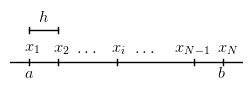
\includegraphics{./cap_pvc/pics/malha_uniforme/malha_uniforme}
  \caption{Malha uniforme de $N$ pontos em um intervalo $[a, b]$.}
  \label{fig:malha_uniforme}
\end{figure}

{\bf 1. Construção da malha.} A malha consiste em uma representação discreta do domínio $[a, b]$. Como veremos, sua construção tem impacto direto nas próximas etapas do método. Aqui, vamos construir a malha mais simples possível, aquela que consiste de $N$ pontos igualmente espaçados, isto é, a chamada \emph{malha uniforme}\index{malha uniforme}.

Para tanto, seja $N\in\mathbb{N}$ dado e, então, tomamos o seguinte conjunto discreto $\mathcal{P}_N = \{x_1, x_2, \dotsc, x_N\}$ (a malha), onde
\begin{equation}
  x_i = a + (i-1)h,\quad i=1, 2, \dotsc, N,
\end{equation}
com
\begin{equation}
  h:=\frac{b-a}{N-1},
\end{equation}
o qual é chamado de \emph{tamanho (ou passo) da malha}\index{tamanho da malha}\index{passo da malha} (veja a Figura~\ref{fig:malha_uniforme}).

{\bf 2. Construção do problema discreto.}\index{problema discreto} A segunda etapa consiste na discretização das equações, no nosso caso, das equações \eqref{eq:pvc1-eq}-\eqref{eq:pvc1-bc2}. 

Vamos começar pela Equação~\eqref{eq:pvc1-eq}. Em um ponto da malha $x_i$, $i = 2, 3, \dotsc, N-1$, temos
\begin{equation}
  -u_{xx}(x_i) = f(x_i, u(x_i)).
\end{equation}
Usando a fórmula de diferenças finitas central de ordem 2 para a segunda derivada, temos
\begin{equation}
  -\left(\frac{u(x_i-h) - 2u(x_i) + u(x_i+h)}{h^2} + O(h^2)\right) = f(x_i, u(x_i)).
\end{equation}
Rearranjando os termos, obtemos
\begin{equation}
  -\frac{u(x_i-h) - 2u(x_i) + u(x_i+h)}{h^2} = f(x_i, u(x_i)) + O(h^2). 
\end{equation}

Agora, denotando por $u_i$ a aproximação numérica de $u(x_i)$, a equação acima nos fornece
\begin{equation}\label{eq:pvc1-disc-eq}
\frac{1}{h^2}u_{i-1} - \frac{2}{h^2}u_i + \frac{1}{h^2}u_{i+1} = -f(x_i, u_i),
\end{equation}
para $i=2, 3, \dotsc, N-1$. Observamos que trata-se de um sistema de $N$ incógnitas, a saber $u_i$, e de $N-2$ equações, isto é, um sistema subdeterminado.

Para obtermos um sistema determinado, aplicamos as condições de contorno. Da condição de contorno dada na Equação~\eqref{eq:pvc1-bc1}, temos
\begin{equation}\label{eq:pvc1-disc-bc1}
  u(a) = u_a\Rightarrow u_1 = u_a.
\end{equation}
Analogamente, da condição de contorno dada na Equação~\eqref{eq:pvc1-bc1}, temos
\begin{equation}\label{eq:pvc1-disc-bc2}
  u(b) = u_b\Rightarrow u_N = u_b.
\end{equation}

Por fim, as equações \eqref{eq:pvc1-disc-bc2}, \eqref{eq:pvc1-disc-eq} e \eqref{eq:pvc1-disc-bc1} determinam o problema discreto associado
\begin{eqnarray}
  u_1 &=& u_a,\label{eq:pvc1-disc-eq1}\\
  \frac{1}{h^2}u_{i-1} - \frac{2}{h^2}u_i + \frac{1}{h^2}u_{i+1} &=& -f(x_i, u_i),\quad i=2, \dotsc, N-1,\label{eq:pvc1-disc-eqi}\\
  u_N &=& u_b.\label{eq:pvc1-disc-eqN}
\end{eqnarray}
Este é um sistema de equações de $N$ incógnitas e $N$ equações.

{\bf 3. Resolução do sistema discreto.} Esta etapa consiste em resolver o sistema discreto construído na etapa anterior. 

Para o PVC \eqref{eq:pvc1-eq}-\eqref{eq:pvc1-bc2}, construímos o problema discreto \eqref{eq:pvc1-disc-eq1}-\eqref{eq:pvc1-disc-eqN}. Este é um problema de $N$ equações e $N$ incógnitas. Observamos que se $f(x, u)$ é uma função linear, o sistema será linear e podemos resolver o sistema usando de técnicas numéricas para sistema lineares. Agora, se $f(x, u)$ é uma função não linear, podemos usar, por exemplo, do método de Newton para sistemas.

{\bf 4. Visualização e interpretação dos resultados.} A solução do problema discreto consiste dos valores $u_i$, isto é, de aproximações dos valores de $u$ nos pontos da malha. Para visualizarmos a solução podemos, por exemplo, construir o gráfico do conjunto de pontos $\{(x_i, u_i)\}$. Ainda, para obtermos aproximações da solução em outros pontos que não fazem parte da malha, podemos usar de técnicas de interpolação e/ou ajuste.

\begin{ex}\label{ex:pvc2}
  Use o método de diferenças finitas para resolver o seguinte problema de valor de contorno com condições de Dirichlet homogêneas:
  \begin{eqnarray}
    -u_{xx} &=& 100(x-1)^2,\quad 0 < x < 1,\label{eq:pvc2-eq}\\
    u(0) &=& 0,\label{eq:pvc2-bc1}\\
    u(1) &=& 0.\label{eq:pvc2-bc2}
  \end{eqnarray}
Use a fórmula de diferenças finitas central de ordem 2 para discretizar a derivada em uma malha uniforme de 11 pontos. Calcule, também, a solução analítica deste problema, faça um esboço das soluções numérica e analítica e compute o erro absoluto médio definido por
\begin{equation}
  E := \frac{1}{N}\sum_{i=1}^N \left|u(x_i) - u_i\right|,
\end{equation}
onde $x_i$ é o $i$-ésimo ponto da malha, $i=1, 2, \dotsc, N$ e $N$ é o número de pontos na mesma. Por fim, repita seus cálculos para uma malha com $101$ pontos. O que ocorre com o erro absoluto médio?
\end{ex}
\begin{sol} Vamos seguir as etapas conforme acima.

  {\bf 1. Construção da malha.} Tomando $N=11$, definimos os pontos da malha no domínio [0, 1] por:
  \begin{equation}
    x_i = (i-1)h,\quad i=1, 2, \dotsc, N,
  \end{equation}
com $h = 1/(N-1)$.

%%%%%%%%%%%%%%%%%%%%
% scilab
%%%%%%%%%%%%%%%%%%%%
\ifisscilab
No \verb+Scilab+, podemos construir a malha da seguinte forma:
\begin{verbatim}
a = 0
b = 1
N = 11
h = (b-a)/(N-1)
x = linspace(a,b,N)
\end{verbatim}
\fi
%%%%%%%%%%%%%%%%%%%%
%%%%%%%%%%%%%%%%%%%%
% octave
%%%%%%%%%%%%%%%%%%%%
\ifisoctave
No \verb+GNU Octave+, podemos construir a malha da seguinte forma:
\begin{verbatim}
a = 0
b = 1
N = 11
h = (b-a)/(N-1)
x = linspace(a,b,N)
\end{verbatim}
\fi
%%%%%%%%%%%%%%%%%%%%
%%%%%%%%%%%%%%%%%%%%
% python
%%%%%%%%%%%%%%%%%%%%
\ifispython
Em \verb+Python+, podemos construir a malha da seguinte forma:
\begin{verbatim}
a = 0
b = 1
N = 11
h = (b-a)/(N-1)
x = np.linspace(a,b,N)
\end{verbatim}
\fi
%%%%%%%%%%%%%%%%%%%%

{\bf 2. Construção do problema discreto.} Usando a fórmula de diferenças finitas central de ordem 2 para aproximar a derivada na Equação~\eqref{eq:pvc2-eq}, obtemos o seguinte sistema de equações:
\begin{equation}
  - \frac{u_{i-1} - 2u_i + u_{i+1}}{h^2} = 100(x_i - 1)^2,\quad i = 2, \dotsc, N-1.
\end{equation}
Completamos este sistema com as condições de contorno dadas nas equações~\eqref{eq:pvc2-bc1} e \eqref{eq:pvc2-bc2}, donde
\begin{equation}
  u_1 = u_N = 0.
\end{equation}
Ou seja, obtemos o seguinte problema discreto:
\begin{eqnarray}
  u_1 &=& 0,\label{eq:pvc2_disc_bc1}\\
  -\frac{1}{h^2}\left(u_{i-1} - 2u_i + u_{i+1}\right) &=& 100(x_i-1)^2,\quad i=2, \dotsc, N-1,\\
  u_N &=& 0.\label{eq:pvc2_disc_bc2}
\end{eqnarray}
Observamos que este é um sistema linear $N\times N$, o qual pode ser escrito na forma matricial $A\underline{u} = b$, cujos matriz de coeficientes é
\begin{equation}
  A = 
  \begin{bmatrix}
    1 & 0 & 0 & 0 & 0 & \cdots & 0\\
    1 & -2 & 1 & 0 & 0 & \cdots & 0\\
    0 & 1 & -2 & 1 & 0 & \cdots & 0\\
    \vdots & \vdots & \vdots & \vdots & \vdots & \vdots & \vdots\\
    0 & 0 & 0 & 0 & 0 & \cdots & 1
  \end{bmatrix},
\end{equation}
o vetor das incógnitas e o vetor dos termos constantes são
\begin{equation}
  \underline{u} =
  \begin{bmatrix}
    u_1\\
    u_2\\
    u_3\\
    \vdots\\
    u_N
  \end{bmatrix}\quad\text{e}\quad
  b =
  \begin{bmatrix}
    0\\
    -100h^{2}(x_2-1)^2\\
    -100h^{2}(x_3-1)^2\\
    \vdots\\
    0
  \end{bmatrix}.
\end{equation}

%%%%%%%%%%%%%%%%%%%%
% scilab
%%%%%%%%%%%%%%%%%%%%
\ifisscilab
No \verb+Scilab+, podemos construir o problema discreto a seguinte forma:
\begin{verbatim}
A = zeros(N,N)
b = zeros(N)

A(1,1) = 1
b(1) = 0
for i = 2:N-1
    A(i,i-1) = 1
    A(i,i) = -2
    A(i,i+1) = 1
    b(i) = -100 * h^2 * (x(i)-1)^2
end
A(N,N) = 1
b(N) = 0
\end{verbatim}
\fi
%%%%%%%%%%%%%%%%%%%%
%%%%%%%%%%%%%%%%%%%%
% octave
%%%%%%%%%%%%%%%%%%%%
\ifisoctave
No \verb+GNU Octave+, podemos construir o problema discreto a seguinte forma:
\begin{verbatim}
A = zeros(N,N)
b = zeros(N)

A(1,1) = 1
b(1) = 0
for i = 2:N-1
    A(i,i-1) = 1
    A(i,i) = -2
    A(i,i+1) = 1
    b(i) = -100 * h^2 * (x(i)-1)^2
end
A(N,N) = 1
b(N) = 0
\end{verbatim}
\fi
%%%%%%%%%%%%%%%%%%%%
%%%%%%%%%%%%%%%%%%%%
% python
%%%%%%%%%%%%%%%%%%%%
\ifispython
Em \verb+Python+, podemos construir o problema discreto a seguinte forma:
\begin{verbatim}
A = np.zeros((N,N))
b = np.zeros(N)

A[0,0] = 1
b[0] = 0
for i in np.arange(1,N-1):
    A[i,i-1] = 1
    A[i,i] = -2
    A[i,i+1] = 1
    b[i] = -100 * h**2 * (x[i]-1)**2
A[N-1,N-1] = 1
b[N-1] = 0
\end{verbatim}
\fi
%%%%%%%%%%%%%%%%%%%%

{\bf 3. Resolução do problema discreto.} Neste caso, o problema discreto consiste no sistema linear $A\underline{u} = b$ e, portanto, a solução é
\begin{equation}\label{eq:pvc2_numerica}
  \underline{u} = A^{-1}b.
\end{equation}

%%%%%%%%%%%%%%%%%%%%
% scilab
%%%%%%%%%%%%%%%%%%%%
\ifisscilab
No \verb+Scilab+, podemos computar a solução do sistema $A\underline{u} = b$ com:
\begin{verbatim}
u = A\b
\end{verbatim}
\fi
%%%%%%%%%%%%%%%%%%%%
%%%%%%%%%%%%%%%%%%%%
% octave
%%%%%%%%%%%%%%%%%%%%
\ifisoctave
No \verb+GNU Octave+, podemos computar a solução do sistema $A\underline{u} = b$ com:
\begin{verbatim}
u = A\b
\end{verbatim}
\fi
%%%%%%%%%%%%%%%%%%%%
%%%%%%%%%%%%%%%%%%%%
% python
%%%%%%%%%%%%%%%%%%%%
\ifispython
Em \verb+Python+, podemos computar a solução do sistema $A\underline{u} = b$ com:
\begin{verbatim}
u = np.linalg.solve(A,b)
\end{verbatim}
\fi
%%%%%%%%%%%%%%%%%%%%

\begin{figure}
  \centering
  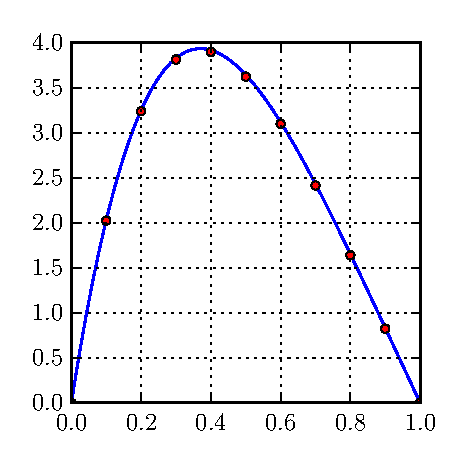
\includegraphics{./cap_pvc/pics/ex_pvc2/ex_pvc2}
  \caption{Esboço dos gráficos das soluções analítica (linha) e numérica (pontos) do PVC dado no Exemplo~\ref{ex:pvc2}.}
  \label{fig:ex_pvc2}
\end{figure}

{\bf 4. Visualização e interpretação dos resultados.} Tendo resolvido o problema discreto $A\underline{u} = b$, obtemos os valores da solução numérico de $u$ nos pontos da malha, isto é, obtivemos o conjunto de pontos $\{(x_i, u_i)\}_{i=1}^N$. Neste exemplo, queremos comparar a solução numérica com a solução analítica.

A solução analítica pode ser obtida por integração. Temos:
\begin{equation}
  \begin{split}
    -u_{xx} = 100(x-1)^2 &\Rightarrow -u_x + c_1 = 100\frac{(x-1)^3}{3}\\
    \Rightarrow -u + c_2x + c_1 = 100\frac{(x-1)^4}{12},
  \end{split}
\end{equation}
ou seja, $\displaystyle u(x) = - \frac{(x-1)^4}{12} + c_2x + c_1$. As constantes são determinadas pelas condições de contorno dadas pelas equações~\eqref{eq:pvc2-bc1} e \eqref{eq:pvc2-bc2}, isto é:
\begin{equation}
  \begin{split}
    u(0) = 0 &\Rightarrow c_1 = \frac{100}{12},\\
    u(1) = 0 &\Rightarrow c_2 = -\frac{100}{12}.
  \end{split}
\end{equation}
Portanto, a solução analítica é:
\begin{equation}\label{eq:pvc2_analitica}
  u(x) = -100\frac{(x-1)^4}{12} - 100\frac{x}{12} + \frac{100}{12}
\end{equation}

A Figura~\ref{fig:ex_pvc2} mostra o esboço dos gráficos das soluções analítica \eqref{eq:pvc2_analitica} e a da solução numérica \eqref{eq:pvc2_numerica}.

%%%%%%%%%%%%%%%%%%%%
% scilab
%%%%%%%%%%%%%%%%%%%%
\ifisscilab
No \verb+Scilab+, podemos fazer o esboço das soluções analítica e numérica da seguinte forma:
\begin{verbatim}
//def. sol. analitica
deff('y = ue(x)','y = -100.0*(x-1).^4/12 - 100*x/12 + 100.0/12')

//gráfico
xx = linspace(0,1)
yy = ue(xx)

plot(x,u,'ro',xx,yy,'b-')
\end{verbatim}
\fi
%%%%%%%%%%%%%%%%%%%%
%%%%%%%%%%%%%%%%%%%%
% octave
%%%%%%%%%%%%%%%%%%%%
\ifisoctave
No \verb+GNU Octave+, podemos fazer o esboço das soluções analítica e numérica da seguinte forma:
\begin{verbatim}
#def. sol. analitica
ue = inline("-100.0*(x-1).^4/12 - 100*x/12 + 100.0/12")

#gráfico
xx = linspace(0,1)
yy = ue(xx)

plot(x,u,'ro',xx,yy,'b-')
\end{verbatim}
\fi
%%%%%%%%%%%%%%%%%%%%
%%%%%%%%%%%%%%%%%%%%
% python
%%%%%%%%%%%%%%%%%%%%
\ifispython
Em \verb+Python+, podemos fazer o esboço das soluções analítica e numérica da seguinte forma:
\begin{verbatim}
#def. sol. analitica
def ue(x):
    return -100.0*(x-1)**4/12 - 100*x/12 + 100.0/12

#gráfico
xx = np.linspace(0,1)
yy = np.zeros(50)
for i,xxi in enumerate(xx):
    yy[i] = ue(xxi)

plt.plot(x',u,'ro',xx,yy,'b-')
plt.show()
\end{verbatim}
\fi
%%%%%%%%%%%%%%%%%%%%

\begin{table}
  \centering
  \caption{Erro absoluto médio das soluções numéricas com $N=11$ e $N=101$ do PVC dado no Exemplo~\ref{ex:pvc2}.}
  \begin{tabular}{ll|c}
    $N$ & $h$ & $E$\\\hline
    11 & 0,1 & $1,3\times 10^{-2}$\\
    101 & 0,01 & $1,4\times 10^{-4}$
  \end{tabular}
  \label{tab:pvc2_erro}
\end{table}

Por fim, computamos o erro absoluto médio das soluções numéricas com $N=11$ e $N=101$. A Tabela~\ref{tab:pvc2_erro} mostra os resultados obtidos. Observamos, que ao diminuirmos $10$ vezes o tamanho do passo $h$, o erro absoluto médio diminui aproximadamente $100$ vezes. Este resultado é esperado, pois o problema discreto \eqref{eq:pvc2_disc_bc1}-\eqref{eq:pvc2_disc_bc2} aproxima o problema contínuo \eqref{eq:pvc2-eq}-\eqref{eq:pvc2-bc2} com erro de truncamento de ordem $h^2$. Verifique!

%%%%%%%%%%%%%%%%%%%%
% scilab
%%%%%%%%%%%%%%%%%%%%
\ifisscilab
No \verb+Scilab+, podemos computar o erro absoluto médio da seguinte forma:
\begin{verbatim}
E = sum(abs(ue(x)' - u))/N
\end{verbatim}
\fi
%%%%%%%%%%%%%%%%%%%%
%%%%%%%%%%%%%%%%%%%%
% octave
%%%%%%%%%%%%%%%%%%%%
\ifisoctave
No \verb+GNU Octave+, podemos computar o erro absoluto médio da seguinte forma:
\begin{verbatim}
E = sum(abs(ue(x)' - u))/N
\end{verbatim}
\fi
%%%%%%%%%%%%%%%%%%%%
%%%%%%%%%%%%%%%%%%%%
% python
%%%%%%%%%%%%%%%%%%%%
\ifispython
Em \verb+Python+, podemos computar o erro absoluto médio da seguinte forma:
\begin{verbatim}
E = 0
for i,xi in enumerate(x):
    E += np.abs(ue(xi) - u[i])
E /= N
\end{verbatim}
\fi
%%%%%%%%%%%%%%%%%%%%
\end{sol}

\subsection*{Exercícios resolvidos}

\begin{exeresol}\label{exeresol:pvc_linear} Use o método de diferenças finitas para resolver o seguinte problema de valor de contorno:
  \begin{eqnarray}
    -u_{xx} + u  &=& e^{-x},\quad 0<x<1,\\
    u(0,5) &=& 1,\\
    u(1,5) &=& 2.
  \end{eqnarray}
Para tanto, use a fórmula de diferenças finitas central de ordem 2 para discretizar a derivada em uma malha uniforme com passo $h=0,1$. Faça, então, um esboço do gráfico da solução computada.
\end{exeresol}
\begin{resol}
O passo $h$ é uma malha uniforme com $N$ pontos no domínio $[0,5, 1,5]$ satisfaz:
\begin{equation}
  h = \frac{(b-a)}{N-1} \Rightarrow N = \frac{(b-a)}{h} + 1.
\end{equation}
Ou seja, a malha deve conter $N = 11$ pontos igualmente espaçados. Denotamos os pontos na malha por $x_i$, onde $x_i = 0,5 + (i-1)h$.

\begin{table}
  \centering
  \begin{tabular}{cc|cc}
    $x$ & $u$ & $x$ & $u$\\\hline
0.50 & 1.000000 & 1.00 & 1.643900 \\
0.60 & 1.143722 & 1.10 & 1.745332 \\
0.70 & 1.280661 & 1.20 & 1.834176 \\
0.80 & 1.410269 & 1.30 & 1.908160 \\
0.90 & 1.531724 & 1.40 & 1.964534 \\
1.00 & 1.643900 & 1.50 & 2.000000 \\\hline
  \end{tabular}
  \caption{Solução numérica do Exercício~\ref{exeresol:pvc_linear}.}
  \label{tab:exeresol_pvc_linear}
\end{table}

Agora, a equação diferencial dada no $i$-ésimo ponto da malha é:
\begin{equation}
  -u_{xx}(x_i) + u(x_i) = e^{x_i},\quad i = 2, 3, \dotsc, N-1.
\end{equation}
Denotando $u_i \approx u(x_i)$ e usando a fórmula de diferenças finitas central de ordem dois para a derivada $u_{xx}$, obtemos:
\begin{equation}
  -\left(\frac{u_{i-1} - 2u_i + u_{i+1}}{h^2}\right) + u_i = e^{x_i},
\end{equation}
para $i= 2, 3, \dotsc, N-1$. Rearranjando os termos e aplicando as condições de contorno, temos o problema discretizado como segue:
\begin{equation}
  \begin{split}
    u_1 &= 1\\
    -u_{i-1} + (2 + h^2)u_i - u_{i+1} &= h^2e^{x_i},\quad i=2 ,\dotsc, N-1,\\
    u_N &= 2.
  \end{split}
\end{equation}

\begin{figure}
  \centering
  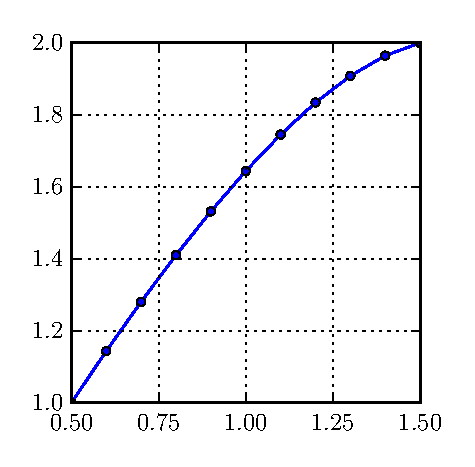
\includegraphics{./cap_pvc/pics/exeresol_pvc_linear/exeresol_pvc_linear}
  \caption{Esboço do gráfico da solução numérica do Exercício~\ref{exeresol:pvc_linear}.}
  \label{fig:exeresol_pvc_linear}
\end{figure}

O problema discreto obtido é um sistema linear $N\times N$. Resolvendo este sistema, obtemos a solução discreta apresentada na Tabela~\ref{tab:exeresol_pvc_linear}. A Figura~\ref{fig:exeresol_pvc_linear} mostra um esboço do gráfico da solução computada.

%%%%%%%%%%%%%%%%%%%%
% scilab
%%%%%%%%%%%%%%%%%%%%
\ifisscilab
No \verb+Scilab+, podemos computar a solução numérica e graficá-la com o seguinte código:
\begin{verbatim}
//malha
a = 0.5
b = 1.5
N = 11
h = (b-a)/(N-1)
x = linspace(a,b,N)'

//sistema
A = zeros(N,N)
b = zeros(N,1)

A(1,1) = 1
b(1) = 1
for i = 2:N-1
    A(i,i-1) = -1
    A(i,i) = 2 + h^2
    A(i,i+1) = -1
    b(i) = h^2 * exp(x(i))
end
A(N,N) = 1
b(N) = 2

//solucao
u = A\b

//gráfico
plot(x,u,'b-o')
\end{verbatim}
\fi
%%%%%%%%%%%%%%%%%%%%
%%%%%%%%%%%%%%%%%%%%
% octave
%%%%%%%%%%%%%%%%%%%%
\ifisoctave
No \verb+GNU Octave+, podemos computar a solução numérica e graficá-la com o seguinte código:
\begin{verbatim}
#malha
a = 0.5
b = 1.5
N = 11
h = (b-a)/(N-1)
x = linspace(a,b,N)'

#sistema
A = zeros(N,N)
b = zeros(N,1)

A(1,1) = 1
b(1) = 1
for i = 2:N-1
    A(i,i-1) = -1
    A(i,i) = 2 + h^2
    A(i,i+1) = -1
    b(i) = h^2 * exp(x(i))
endfor
A(N,N) = 1
b(N) = 2

#solucao
u = A\b

#gráfico
plot(x,u,'b-o')
\end{verbatim}
\fi
%%%%%%%%%%%%%%%%%%%%
%%%%%%%%%%%%%%%%%%%%
% python
%%%%%%%%%%%%%%%%%%%%
\ifispython
Em \verb+Python+, podemos computar a solução numérica e graficá-la com o seguinte código:
\begin{verbatim}
#malha
a = 0.5
b = 1.5
N = 11
h = (b-a)/(N-1)
x = np.linspace(a,b,N)

#sistema
A = np.zeros((N,N))
b = np.zeros(N)

A[0,0] = 1
b[0] = 1
for i in np.arange(1,N-1):
    A[i,i-1] = -1
    A[i,i] = 2 + h**2
    A[i,i+1] = -1
    b[i] = h**2 * np.exp(x[i])
A[N-1,N-1] = 1
b[N-1] = 2

#solucao
u = np.linalg.solve(A,b)

#gráfico
plt.plot(x,u,'b-o')
plt.show()
\end{verbatim}
\fi
%%%%%%%%%%%%%%%%%%%%
\end{resol}

\subsection*{Exercícios}

\begin{exer}
 Considere o seguinte problema de valor de contorno para a equação de calor no estado estacionário:
\begin{equation}\left\{\begin{array}{l}-u_{xx}=32,~~ 0<x<1.\\
u(0)=5\\
u(1)=10\end{array}
\right.
\end{equation}

Defina $u_j=u(x_j)$ onde $x_j={(j-1)}{h}$ e $j=1,\ldots,5$. Aproxime a derivada segunda por um esquema de segunda ordem e transforme a equação diferencial em um sistema de equações lineares. Escreva este sistema linear na forma matricial e resolva-o. Faça o mesmo com o dobro de subintervalos, isto é, com malha de 9 pontos. 
\end{exer}
\begin{resp}
 \begin{equation}\left[
  \begin{array}{ccccc}
         1 & 0& 0& 0& 0\\
         -1 & 2 & -1 &0&0\\
         0&-1 & 2 & -1 &0\\
         0&0&-1 & 2 & -1 \\
         0 & 0& 0& 0& 1\\
        \end{array}
\right]
\left[
  \begin{array}{c}
     u_1\\ u_2\\u_3\\u_4 \\ u_5
   \end{array}
\right]
=
\left[
  \begin{array}{c}
     5\\ 2\\2\\2 \\ 10
   \end{array}
\right]
\end{equation}


Solução:  [5, 9.25, 11.5, 11.75, 10]    

\begin{equation}\left[
  \begin{array}{ccccccccc}
         1 & 0& 0& 0& 0& 0& 0& 0& 0\\
         -1 & 2 & -1 &0&0& 0& 0& 0& 0\\
         0&-1 & 2 & -1 &0& 0& 0& 0& 0\\
         0&0&-1 & 2 & -1 & 0& 0& 0& 0\\
         0&0&0&-1 & 2 & -1 & 0& 0& 0\\
         0&0&0&0&-1 & 2 & -1 & 0& 0\\
         0&0&0&0&0&-1 & 2 & -1 & 0\\
         0&0&0&0&0&0&-1 & 2 & -1\\
         0 & 0& 0& 0& 0& 0& 0& 0& 1\\
        \end{array}
\right]
\left[
  \begin{array}{c}
     u_1\\ u_2\\u_3\\u_4 \\u_5\\ u_6\\u_7\\u_8\\u_9
   \end{array}
\right]
=
\left[
  \begin{array}{c}
     5\\ 0.5\\0.5\\0.5\\ 0.5\\0.5\\0.5\\0.5 \\ 10
   \end{array}
\right]
\end{equation}

Solução:  $[5, 7.375, 9.25, 10.625, 11.5, 11.875, 11.75, 1.125, 10]$
\end{resp}


\begin{exer} Considere o seguinte problema de valor de contorno para a equação de calor no estado estacionário:
\begin{equation}\left\{\begin{array}{l}-u_{xx}=200e^{-(x-1)^2},~~ 0<x<2.\\
u(0)=120\\
u(2)=100\end{array}
\right.
\end{equation}
Defina $u_j=u(x_j)$ onde $x_j={(j-1)}{h}$ e $j=1,\ldots,21$. Aproxime a derivada segunda por um esquema de segunda ordem e transforme a equação diferencial em um sistema de equações lineares. Resolva o sistema linear obtido.
\end{exer}
\begin{resp}
120.    133.56    146.22    157.83    168.22    177.21    184.65    190.38    194.28    196.26    196.26    194.26    190.28    184.38    176.65    167.21  156.22    143.83    130.22    115.56    100.    
\end{resp}

\begin{exer} Considere o seguinte problema de valor de contorno para a equação de calor no estado estacionário:
\begin{equation}\left\{\begin{array}{l}-u_{xx}=200e^{-(x-1)^2},~~ 0<x<2.\\
u'(0)=0\\
u(2)=100\end{array}
\right.
\end{equation}
Defina $u_j=u(x_j)$ onde $x_j={(j-1)}{h}$ e $j=1,\ldots,21$. Aproxime a derivada segunda por um esquema de segunda ordem, a derivada primeira na fronteira por um esquema de primeira ordem e transforme a equação diferencial em um sistema de equações lineares. Resolva o sistema linear obtido.
\end{exer}
\begin{resp}
391.13    391.13    390.24    388.29    385.12    380.56    374.44    366.61    356.95    345.38    331.82    316.27    298.73    279.27    257.99    234.99    210.45    184.5    157.34    129.11    100.    
\end{resp}


\begin{exer} Considere o seguinte problema de valor de contorno para a equação de calor no estado estacionário com um termo não linear de radiação:
\begin{equation}\left\{\begin{array}{l}-u_{xx}=100- \frac{u^4}{10000},~~ 0<x<2.\\
u(0)=0\\
u(2)=10\end{array}
\right.
\end{equation}
Defina $u_j=u(x_j)$ onde $x_j={(j-1)}{h}$ e $j=1,\ldots,21$. Aproxime a derivada segunda por um esquema de segunda ordem e transforme a equação diferencial em um sistema de equações não lineares. Resolva o sistema  obtido. Expresse  a solução com dois algarismos depois do separador decimal. Dica: Veja problema 38 da lista 2, seção de sistemas não lineares.
\end{exer}
\begin{resp}
0.,    6.57,    12.14,    16.73,    20.4,    23.24,    25.38,    26.93 ,   28,    28.7,    29.06,    29.15,    28.95,    28.46, 27.62 ,   26.36,    24.59,    22.18,    19.02,    14.98,    10.    
\end{resp}

\begin{exer} Considere o seguinte problema de valor de contorno para a equação de calor no estado estacionário com um termo não linear de radiação e um termo de convecção:
\begin{equation}\left\{\begin{array}{l}-u_{xx}+3u_x=100- \frac{u^4}{10000},~~ 0<x<2.\\
u'(0)=0\\
u(2)=10\end{array}
\right.
\end{equation}
Defina $u_j=u(x_j)$ onde $x_j={(j-1)}{h}$ e $j=1,\ldots,21$. Aproxime a derivada segunda por um esquema de segunda ordem, a derivada primeira na fronteira por um esquema de primeira ordem, a derivada primeira no interior por um esquema de segunda ordem e transforme a equação diferencial em um sistema de equações não lineares. Resolva o sistema  obtido.
\end{exer}
\begin{resp}
$u(0)=31.62$, $u(1)=31,50$, $u(1,9)=18,17$.    
\end{resp}

\begin{exer} Considere o seguinte problema de valor de contorno:
\begin{equation}\left\{\begin{array}{l}-u''+2u'=e^{-x}- \frac{u^2}{100},~~ 1<x<4.\\
u'(1)+u(1)=2\\
u'(4)=-1\end{array}
\right.
\end{equation}
Defina $u_j=u(x_j)$ onde $x_j=1+{(j-1)}{h}$ e $j=1,\ldots,101$. Aproxime a derivada segunda por um esquema de segunda ordem, a derivada primeira na fronteira por um esquema de primeira ordem, a derivada primeira no interior por um esquema de segunda ordem e transforme a equação diferencial em um sistema de equações não lineares. Resolva o sistema  obtido.
\end{exer}
\begin{resp}
$u(1)=1,900362$, $u(2,5)=1.943681$, $u(4)=1,456517$.    
\end{resp}

%\end{document} 


%%%%%%%%%%%%%%%%%%%%
% scilab
%%%%%%%%%%%%%%%%%%%%
\ifisscilab
\appendix
\include{./cap_scilab/cap_scilab}
\fi
%%%%%%%%%%%%%%%%%%%%
%%%%%%%%%%%%%%%%%%%%
% octave
%%%%%%%%%%%%%%%%%%%%
\ifisoctave
\appendix
%Este trabalho está licenciado sob a Licença Creative Commons Atribuição-CompartilhaIgual 3.0 Não Adaptada. Para ver uma cópia desta licença, visite https://creativecommons.org/licenses/by-sa/3.0/ ou envie uma carta para Creative Commons, PO Box 1866, Mountain View, CA 94042, USA.

\chapter{Rápida Introdução ao GNU Octave}\label{cap:octave}\index{GNU Octave}

Neste apêndice, discutiremos os principais aspectos da linguagem computacional \verb+GNU Octave+ que são essenciais para uma boa leitura desta versão do livro. O material aqui apresentado, é uma adaptação livre do apêndice A de \cite{CALSCI}.

\section{Sobre o GNU Octave}\index{Octave!sobre}

\verb+GNU Octave+ é uma linguagem computacional de alto nível para computação numérica. \verb+GNU Octave+ é distribuído livremente sobre licença GPL. A linguagem acompanha um GUI (Interface Gráfica do Utilizador) em versões para Linux, Mac, BSD e Windows. 

Para mais informações sobre o GNU Octave, visite sua página oficial
\begin{center}
  \url{https://www.gnu.org/software/octave/}
\end{center}

O manual oficial do GNU Octave pode ser obtido em:
\begin{center}
  \url{https://www.gnu.org/software/octave/doc/interpreter/}
\end{center}

\section{Instalação e Execução}\index{GNU Octave!instalação e execução}

O \verb+GNU Octave+ pode ser executado normalmente nos sistemas operacionais Linux, Mac Os, BSD e Windows . Muitas distribuições de Linux (Linux Mint, Ubuntu, etc.) têm o \verb+GNU Octave+ no seu sistema de pacotes (incluindo binário e documentação). Alternativamente, no \href{https://www.gnu.org/software/octave/}{site oficial do GNU Octave} pode-se obter mais versões de binários e documentação para instalação.

\section{Usando o GNU Octave}\index{GNU Octave!usando}

O uso do \verb+GNU Octave+ pode ser feito de três formas básicas:
\begin{itemize}
\item usando o {\bf console} de modo iterativo;
\item usando a função \verb+run+ para executar um código GNU Octave digitado em um arquivo externo;
\item usando processamento {\it bash}.
\end{itemize}

\begin{ex}
  Considere o seguinte pseudocódigo:
\begin{verbatim}
s = "Olá, mundo!". (Sem imprimir na tela o resultado.)
saída(s). (Imprime na tela.)
\end{verbatim}
Implemente este pseudocódigo no GNU Octave: a) usando somente o console do \verb+GNU Octave+; b) usando o editor do \verb+GNU Octave+ e executando o código com a função \verb+exec+; c) usando processamento {\it bash}.
\end{ex}
\begin{sol} Seguem as soluções de cada item:
  \begin{itemize}
  \item[a)]  No console temos:
\begin{verbatim}
>> x = "Olá, mundo\n";
>> disp(x)
\end{verbatim}
  \item[b)] O GUI do \verb+GNU Octave+ disponibiliza um editor para {\it scripts} que ser acessado digitando-se no \verb+prompt+:
\begin{verbatim}
-->edit
\end{verbatim}
Então, digita-se no editor o código:
\begin{verbatim}
x = "Olá, mundo!\n";
disp(x);
\end{verbatim}
salva-se em um arquivo de sua preferência com extensão \verb+.m+ (por exemplo, \verb+~/ola.m+) e executa-se o código clicando no botão ``{\it play}'' disponível na barra de botões do editor.
\item[c)] Para executar o código em processamento {\it bash}, digita-se em um editor o código:
\begin{verbatim}
x = "Olá, mundo!\n";
disp(x);
\end{verbatim}
salva-se em um arquivo de sua preferência com extensão \verb+.m+ (por exemplo, \verb+~/ola.m+) e executa-se em um console do sistema usando a linha de comando:
\begin{verbatim}
$ octave ~/ola.m
\end{verbatim}
\end{itemize}
\end{sol}

\section{Elementos da linguagem}\index{GNU Octave!elementos da linguagem}

\verb+GNU Octave+ é uma linguagem interpretada em que as variáveis são matrizes. Uma variável é criada quando um valor é atribuído a ela. Por exemplo:
\begin{verbatim}
>> x=1
x =  1
>> y = x * 2
y =  2  
\end{verbatim}
a variável \verb+x+ recebe o valor \verb+double+ $1$ e, logo após, na segunda linha de comando, a variável \verb+y+ recebe o valor \verb+double+ $2$. Observamos que o símbolo \verb+=+ significa o operador de atribuição não o de igualdade. O operador lógico de igualdade no \verb+GNU Octave+ é \verb+==+.

Comentários e continuação de linha de comando são usados como no seguinte exemplo:
\begin{verbatim}
>> #Isto é um comentário
>> x = 1 ...
+ 2
x =  3  
\end{verbatim}

\subsection{Operações matemáticas elementares}\index{GNU Octave!operações matemáticas}

No \verb+GNU Octave+, os operadores matemáticos elementares são os seguintes:
\begin{verbatim}
  + adição
  - subtração
  * multiplicação
  / divisão
  ^ potenciação
  ' transposto conjugado
\end{verbatim}

\subsection{Funções e constantes elementares}\index{GNU Octave!funções e constantes}

Várias funções e constantes elementares já estão pré-definidas no \verb+GNU Octave+. Por exemplo:
\begin{verbatim}
>> cos(pi) #cosseno de pi
ans = -1
>> sin(pi) #seno de pi
ans =    1.2246e-16
>> exp(1) == e
ans =  1
>> log(e) #logarítmo natural
ans =  1
\end{verbatim}

\subsection{Operadores lógicos}\index{Octave!operadores lógicos}

No \verb+GNU Octave+, o valor lógico verdadeiro é escrito como \verb+true+ e o valor lógico falso como \verb+false+. Temos os seguintes operadores lógicos disponíveis:
\begin{verbatim}
&  e lógico
|  ou lógico
!  negação
== igualdade
!= diferente
<  menor que
>  maior que
<= menor ou igual que
>= maior ou igual que
\end{verbatim}

\begin{ex}
  Se $x=2$, então $x$ é maior ou igual a 1 e menor que 3? 
\end{ex}
\begin{sol}
  No \verb+GNU Octave+, temos:
\begin{verbatim}
>> x=2;
>> (x >= 1) & (x < 3)
ans =  1
\end{verbatim}
\end{sol}

\section{Matrizes}\index{Octave!matrizes}

No \verb+GNU Octave+, matriz é o tipo básico de dados, a qual é definida por seu número de linhas, colunas e tipo de dado (real, inteiro, lógico, etc.). Uma matriz $A = [a_{i,j}]_{i,j=1}^{m,n}$ no \verb+GNU Octave+ é definida usando-se a seguinte sintaxe:
\begin{verbatim}
A = [ a11 , a12 , ... , a1n ; ...; am1 , am2 , ... , amn ]
\end{verbatim}

\begin{ex}
  Defina a matriz:
  \begin{equation}
    A = \left[
      \begin{array}{ccc}
        1 & 2 & 3\\
        4 & 5 & 6
      \end{array}
\right]
  \end{equation}
\end{ex}
\begin{sol}
  No \verb+GNU Octave+, digitamos:
\begin{verbatim}
>> A = [1 , 2 , 3 ; 4 , 5 , 6]
A =
   1   2   3
   4   5   6
\end{verbatim}
\end{sol}

A seguinte lista contém uma série de funções que geram matrizes particulares:
\begin{verbatim}
eye      matriz identidade
linspace vetor de elementos linearmente espaçados
ones     matriz cheia de uns
zeros    matriz nula
\end{verbatim}

\subsection{O operador ``:''}\index{GNU Octave!operador :}

O operador ``:'' cria um vetor linha de elementos. A sintaxe:
\begin{verbatim}
v = i:s:j
\end{verbatim}
cria um vetor linha:
\begin{equation}
  v = [i,~i+s,~i+2s,\dotsc, i+ns]
\end{equation}
onde $n$ é o maior inteiro tal que $i + ns \leq j$.

\begin{ex}
Veja as seguintes linhas de comando:
\begin{verbatim}
>> u = 2:6
u =
   2   3   4   5   6
>> v = 10:-2:3
v =
   10    8    6    4
\end{verbatim}
\end{ex}

\subsection{Obtendo dados de uma matriz}

A função \verb+size+ retorna as dimensões de uma matriz, por exemplo:
\begin{verbatim}
>> A = ones(3,2)
A =
   1   1
   1   1
   1   1 
>> [nl, nc] = size(A)
nl =  3
nc =  2
\end{verbatim}
informando que a matriz \verb+A+ tem três linhas e duas colunas.

Existem vários métodos para acessar os elementos de uma matriz dada \verb+A+:
\begin{itemize}
\item a matriz inteira acessa-se com a sintaxe:
\begin{verbatim}
A
\end{verbatim}
\item o elemento da $i$-ésima linha e $j$-ésima coluna acessa-se usando a sintaxe:
\begin{verbatim}
A(i,j)
\end{verbatim}
\item o bloco formado pelas linhas $i_1$, $i_2$ e pelas colunas $j_1$, $j_2$ obtém-se usando a sintaxe:
\begin{verbatim}
A(i1:i2, j1:j2)
\end{verbatim}
\end{itemize}

\begin{ex}
  Veja as seguintes linhas de comando:
\begin{verbatim}
>> A = rand(3,4)
A =
   0.356041   0.896038   0.761722   0.447774
   0.453682   0.071638   0.029215   0.500115
   0.885188   0.387276   0.566189   0.683588
>> A
A =
   0.356041   0.896038   0.761722   0.447774
   0.453682   0.071638   0.029215   0.500115
   0.885188   0.387276   0.566189   0.683588
>> A(2,3)
ans =  0.029215
>> A(2:3,2:4)
ans =
   0.071638   0.029215   0.500115
   0.387276   0.566189   0.683588
\end{verbatim}
\end{ex}

Definida uma matriz $A$ no \verb+GNU Octave+, as seguintes sintaxes são bastante úteis:
\begin{verbatim}
A(:,:)   toda a matriz
A(i:j,k) os elementos das linhas i até j (inclusive) da k-ésima coluna
A(i,j:k) os elementos da i-ésima linha das colunas j até k (inclusive)
A(i,:)   a i-ésima linha da matriz
A(:,j)   a j-ésima coluna da matriz
A(i,end) o elemento da i-ésima linha e da última coluna
A(end,j) o elemento da última linha e da j-ésima coluna
\end{verbatim}

\begin{ex}
Veja as seguintes linhas de comando:
\begin{verbatim}
>> B = rand(4,4)
B =

   0.246251   0.931915   0.094609   0.519181
   0.926740   0.898039   0.377078   0.260630
   0.133661   0.652755   0.670097   0.390773
   0.379430   0.314611   0.829729   0.484622

>> aux=B(:,2); B(:,2)=B(:,3); B(:,3)=aux
B =

   0.246251   0.094609   0.931915   0.519181
   0.926740   0.377078   0.898039   0.260630
   0.133661   0.670097   0.652755   0.390773
   0.379430   0.829729   0.314611   0.484622
\end{verbatim}
\end{ex}

\subsection{Operações matriciais e elemento-a-elemento}

As operações matriciais elementares seguem a mesma sintaxe que as operações elementares de números. Agora, no \verb+GNU Octave+, também podemos fazer operações elemento-a-elemento colocando um ponto ``.'' antes da operação desejada.

Aqui, temos as sintaxes análogas entre operações matriciais e operações elemento-a-elemento:
\begin{verbatim}
+ adição               .+ adição elemento-a-elemento
- subtração            .- subtração elemento-a-elemento
* multiplicação        .* multiplicação elemento-a-elemento
                       ./ divisão elemento-a-elemento
^ potenciação          .^ potenciação elemento-a-elemento
' transposta conjugada .' transposta (não conjugada)
\end{verbatim}

\begin{ex}
  Veja as seguintes linhas de comando:
\begin{verbatim}
>> A = ones (2,2)
A =
   1   1
   1   1

>> B = 2 * ones(2, 2)
B =
   2   2
   2   2

>> A * B
ans =
   4   4
   4   4

>> A .* B
ans =
   2   2
   2   2
\end{verbatim}
\end{ex}

\section{Estruturas de ramificação e repetição}\index{Octave!ramificação e repetição}

O \verb+GNU Octave+ contém estruturas de repetição e ramificação padrões de linguagens estruturadas.

\subsection{A instrução de ramificação ``if''}

A instrução ``if'' permite executar um pedaço do código somente se uma dada condição for satisfeita.

\begin{ex}
  Veja o seguinte código \verb+GNU Octave+:
\begin{verbatim}
i = 2;
if ( i == 1 )
    disp ( " Hello ! " );
elseif ( i == 2 )
    disp ( " Goodbye ! " );
elseif ( i == 3 )
    disp ( " Tchau ! " );
else
    disp ( " Au Revoir ! " );
endif
\end{verbatim}
Qual é a saída apresentada no console do \verb+GNU Octave+? Por quê?
\end{ex}

\subsection{A instrução de repetição ``for''}

A instrução \verb+for+ permite que um pedaço de código seja executado repetidamente.

\begin{ex}
  Veja o seguinte código:
\begin{verbatim}
for i = 1:5
    disp(i);
endfor
\end{verbatim}
O que é mostrado no console do \verb+GNU Octave+?
\end{ex}

\begin{ex}
  Veja o seguinte código:
\begin{verbatim}
for j = 1:2:8
    disp(j);
endfor
\end{verbatim}
O que é mostrado no console do \verb+GNU Octave+?
\end{ex}

\begin{ex}
  Veja o seguinte código:
\begin{verbatim}
for k = 10:-3:1
    disp(k);
endfor
\end{verbatim}
O que é mostrado no console do \verb+GNU Octave+?
\end{ex}

\begin{ex}
  Veja o seguinte código:
\begin{verbatim}
for i = 1:3
    for j = 1:3
        disp([i,j]);
    endfor
endfor
\end{verbatim}
O que é mostrado no console do \verb+GNU Octave+?
\end{ex}

\subsection{A instrução de repetição ``while''}

A instrução \verb+while+ permite que um pedaço de código seja executado repetidamente até que uma dada condição seja satisfeita.

\begin{ex}
Veja o seguinte código \verb+GNU Octave+:
\begin{verbatim}
s = 0;
i = 1;
while ( i <= 10 )
   s = s + i;
   i = i + 1;
endwhile
\end{verbatim}
Qual é o valor de \verb+s+ ao final da execução? Por quê?
\end{ex}

\section{Funções}\index{GNU Octave!funções}

Além das muitas funções já pré-definidas no \verb+GNU Octave+, podemos definir nossas próprias funções usando:
\begin{itemize}
\item \verb+Anonymous functions+
\item \verb+Functions (script)+
\end{itemize}

Definir uma função como \emph{anonymous function} é apropriada para funções com poucas instruções. Quando a função exige uma grande quantidade de código para ser definida, a melhor opção é usar a instrução \verb+function+. Veja os seguintes exemplos:

\begin{ex}
  O seguinte código:
\begin{verbatim}
>> f = @(x) x + sin(x)
f =
@(x) x + sin (x)
\end{verbatim}
define, no \verb+GNU Octave+, a função $f(x) = x + \sen x$.

Observe que $f(\pi) = \pi$. Confirme isso computando:
\begin{verbatim}
>> f(pi)
ans =  3.1416
\end{verbatim}
no \verb+GNU Octave+.

Alternativamente, definimos a mesma função com o código:
\begin{verbatim}
function [y] = f(x)
   y = x + sin(x);
endfunction
\end{verbatim}
Verifique!
\end{ex}

\begin{obs}
  Um {\it script} (por exemplo, \verb+CAMINHO/foo.m+) contendo apenas a declaração de uma função pode ser usado no prompt via o comando \verb+run+:
\begin{verbatim}
>> run "CAMINHO/foo.m"
\end{verbatim}
\end{obs}

\begin{ex}
  O seguinte código \verb+GNU Octave+:
\begin{verbatim}
function [z] = h(x,y)
   if (x < y)
      z = y - x;
   else
      z = x - y;
   endif
endfunction
\end{verbatim}
define a função:
\begin{equation}
  h(x,y) = \left\{
    \begin{array}{ll}
      y - x &, x < y\\
      x - y &, x \geq y
    \end{array}
\right.
\end{equation}
Verifique!
\end{ex}

\begin{ex}
  O seguinte código:
\begin{verbatim}
function [y] = J(x)
   y(1,1) = 2*x(1);
   y(1,2) = 2*x(2);

   y(2,1) = -x(2)*sin(x(1)*x(2));
   y(2,2) = -x(1)*sin(x(1)*x(2));
endfunction
\end{verbatim}
define a matriz jacobiana $J(x_1,x_2) := \frac{\p(f_1,f_2)}{\p(x_1,x_2)}$ da função:
\begin{equation}
  f(x_1,x_2) = (x_1^2 + x_2^2,~\cos(x_1x_2)).
\end{equation}
\end{ex}

\begin{ex}
  O seguinte código:
\begin{verbatim}
function [a,b] = v(x,y)
   if (x > y)
     a = 1;
     b = 2;
     return;
   else
     a = 2;
     b = 1;
     return;
   end
endfunction
\end{verbatim}
define a função $v$ que toma duas variáveis e retorna duas variáveis. Por exemplo:
\begin{verbatim}
>> [i,j] = v(3,2)
i =  1
j =  2
\end{verbatim}
\end{ex}

\section{Gráficos}\index{GNU Octave!gráficos}

Para criar um esboço do gráfico de uma função de uma variável real $y = f(x)$, podemos usar a função \verb+plot+. Esta função faz uma representação gráfica de pontos $(x_i, y_i)$ fornecidos. O \verb+GNU Octave+ oferece uma série de opções para esta função de forma que o usuário pode ajustar várias questões de visualização. Consulte sobre a função \verb+plot+ usando a ferramenta de ajuda do \verb+GNU Octave+:
\begin{verbatim}
>> help plot
\end{verbatim}

\begin{ex}
  Veja as seguintes linhas de código:
\begin{verbatim}
>> f = @(x) x .^3 + 1
>> xx = linspace(-2,2);
>> plot(xx,f(xx)); grid on
\end{verbatim}
\end{ex}

\fi
%%%%%%%%%%%%%%%%%%%%
%%%%%%%%%%%%%%%%%%%%
% python
%%%%%%%%%%%%%%%%%%%%
\ifispython
\appendix
\include{./cap_python/cap_python}
\fi
%%%%%%%%%%%%%%%%%%%%

%resposta dos exercícios
\ifishtml
\else
%Este trabalho está licenciado sob a Licença Creative Commons Atribuição-CompartilhaIgual 3.0 Não Adaptada. Para ver uma cópia desta licença, visite https://creativecommons.org/licenses/by-sa/3.0/ ou envie uma carta para Creative Commons, PO Box 1866, Mountain View, CA 94042, USA.

\chapter*{Resposta dos Exercícios}
\addcontentsline{toc}{chapter}{Respostas dos Exercícios}
\fancyhead[RE]{Cálculo Numérico}
\fancyhead[LO]{RESPOSTAS DOS EXERCÍCIOS}
\fancyhead[LE,RO]{\thepage}

Recomendamos ao leitor o uso criterioso das respostas aqui apresentadas. Devido a ainda muito constante atualização do livro, as respostas podem conter imprecisões e erros.
\shipoutAnswer

\fi

%references
\nocite{*}
\bibliographystyle{plain}
\bibliography{main}
\addcontentsline{toc}{chapter}{Referências Bibliográficas}
\fancyhead[RE]{Cálculo Numérico}
\fancyhead[LO]{REFERÊNCIAS BIBLIOGRÁFICAS}
\fancyhead[LE,RO]{\thepage}

\ifishtml
\else
\clearpage
\addcontentsline{toc}{chapter}{Índice Remissivo}
\fancyhead[RE]{Cálculo Numérico}
\fancyhead[LO]{ÍNDICE REMISSIVO}
\fancyhead[LE,RO]{\thepage}
\printindex
\fi

\end{document}
